\documentclass[aspectratio=169,10pt]{ctexbeamer}
% 格点 QCD 千页课程统一样式。由所有分卷与全集共同输入。
\usepackage{amsmath,amssymb,mathtools,bm}
\usepackage{booktabs,tabularx,array}
\usepackage{longtable}
\usepackage{tikz}
\usetikzlibrary{arrows.meta,positioning,calc,fit,shapes.geometric}
\usepackage{pgfplots}
\pgfplotsset{compat=1.17}
\usepackage{graphicx}
\usepackage{adjustbox}
\usepackage{listings}
\usepackage{xcolor}
\usepackage{microtype}
\usepackage{hyperref}

\definecolor{courseblue}{HTML}{17365D}
\definecolor{coursecyan}{HTML}{147D92}
\definecolor{coursegreen}{HTML}{1E7A46}
\definecolor{courseorange}{HTML}{B85C00}
\definecolor{coursered}{HTML}{A62C2B}
\definecolor{coursepurple}{HTML}{6A3D9A}
\definecolor{coursemuted}{HTML}{5B6573}
\definecolor{coursepanel}{HTML}{F3F6F9}
\definecolor{courseline}{HTML}{C9D3DF}

\setbeamersize{text margin left=0.56cm,text margin right=0.56cm}
\setlength{\emergencystretch}{2em}
\setbeamertemplate{navigation symbols}{}
\setbeamertemplate{blocks}[rounded][shadow=false]
\setbeamercolor{normal text}{fg=black!86,bg=white}
\setbeamercolor{structure}{fg=courseblue}
\setbeamercolor{frametitle}{fg=courseblue,bg=white}
\setbeamercolor{block title}{fg=courseblue,bg=coursepanel}
\setbeamercolor{block body}{fg=black!86,bg=coursepanel}
\setbeamercolor{alerted text}{fg=coursered}
\setbeamerfont{frametitle}{size=\large,series=\bfseries}
\setbeamerfont{normal text}{size=\normalsize}
\setbeamertemplate{frametitle}{\vskip0.10cm\insertframetitle\par\vskip0.06cm}
\setbeamertemplate{footline}{%
  \hbox{\begin{beamercolorbox}[wd=\paperwidth,ht=2.3ex,dp=0.9ex,
    leftskip=0.56cm,rightskip=0.56cm]{author in head/foot}%
    \scriptsize\color{coursemuted}\insertshortauthor\hfill
    \insertshorttitle\hfill\insertframenumber/\inserttotalframenumber
  \end{beamercolorbox}}}

\hypersetup{unicode=true,colorlinks=true,linkcolor=courseblue,urlcolor=coursecyan}

\newcommand{\CourseAnchor}[2]{\hypertarget{#1:#2}{}}
\newcommand{\CourseID}[2]{\textcolor{courseblue}{\bfseries #1~#2}}
\newcommand{\CourseRef}[2]{\hyperlink{#1:#2}{\textcolor{coursecyan}{#1~#2}}}
\newcommand{\FrameAnchor}[1]{\CourseAnchor{Fr}{#1}}
\newcommand{\KnowledgeID}[1]{\CourseAnchor{K}{#1}\CourseID{K}{#1}}
\newcommand{\DefinitionID}[1]{\CourseAnchor{Def}{#1}\CourseID{Def}{#1}}
\newcommand{\EquationID}[1]{\CourseAnchor{Eq}{#1}\CourseID{Eq}{#1}}
\newcommand{\DerivationID}[1]{\CourseAnchor{Der}{#1}\CourseID{Der}{#1}}
\newcommand{\TheoremID}[1]{\CourseAnchor{Thm}{#1}\CourseID{Thm}{#1}}
\newcommand{\FigureID}[1]{\CourseAnchor{Fig}{#1}\CourseID{Fig}{#1}}
\newcommand{\TableID}[1]{\CourseAnchor{Tbl}{#1}\CourseID{Tbl}{#1}}
\newcommand{\AlgorithmID}[1]{\CourseAnchor{Alg}{#1}\CourseID{Alg}{#1}}
\newcommand{\ExerciseID}[1]{\CourseAnchor{Ex}{#1}\CourseID{Ex}{#1}}
\newcommand{\SolutionID}[1]{\CourseAnchor{Sol}{#1}\CourseID{Sol}{#1}}
\newcommand{\SourceID}[1]{\CourseAnchor{Src}{#1}\CourseID{Src}{#1}}
\newcommand{\SympyID}[1]{\CourseAnchor{SYM}{#1}\CourseID{SYM}{#1}}

\newcommand{\StatusImplemented}{\textcolor{coursemuted}{接口存在}}
\newcommand{\StatusTested}{\textcolor{coursecyan}{测试通过}}
\newcommand{\StatusClosed}{\textcolor{coursegreen}{方案闭合}}
\newcommand{\StatusPhysical}{\textcolor{coursepurple}{真实数据验证}}
\newcommand{\StatusUnverified}{\textcolor{courseorange}{未验证}}

\newcommand{\SourceLine}[1]{%
  \vspace{0.04em}\par{\raggedright\scriptsize\color{coursemuted}来源：#1\par}}

\newcommand{\BoundaryLine}[1]{%
  \vspace{0.04em}\par{\raggedright\scriptsize\color{courseorange}适用边界：#1\par}}

\newcommand{\PhysicalFlow}[4]{%
  \begin{center}
  \begin{tikzpicture}[node distance=0.42cm and 0.42cm]
    \tikzset{courseflow/.style={draw=coursecyan,fill=coursecyan!7,
      rounded corners=2pt,align=center,text width=3.15cm,minimum height=0.84cm,
      font=\small,inner sep=3pt},
      coursearrow/.style={-{Latex[length=2mm]},draw=courseblue,semithick}}
    \node[courseflow] (a) {#1};
    \node[courseflow,right=of a] (b) {#2};
    \node[courseflow,right=of b] (c) {#3};
    \draw[coursearrow] (a) -- (b);
    \draw[coursearrow] (b) -- (c);
  \end{tikzpicture}
  \par\vspace{0.08cm}{\scriptsize\color{coursemuted}\FigureID{#4}：概念关系示意；颜色只辅助分层。}
  \end{center}}

\newcommand{\CheckMark}{\textcolor{coursegreen}{\bfseries\ensuremath{\checkmark}}}
\newcommand{\RiskMark}{\textcolor{courseorange}{\bfseries !}}
\newcommand{\CodePath}[1]{\texttt{\detokenize{#1}}}
\newsavebox{\CourseEquationMeasureBox}
\newcommand{\CourseDisplayEquation}[1]{%
  \sbox{\CourseEquationMeasureBox}{$\displaystyle #1$}%
  \ifdim\wd\CourseEquationMeasureBox>1.30\linewidth
    \PackageError{lqcd-course}{Main equation would be scaled below the readability floor}%
      {Split the equation with aligned/gathered at a mathematical boundary; do not hide it with tiny text.}%
  \fi
  \begin{adjustbox}{max width=0.96\linewidth,max totalheight=0.16\textheight}%
    $\displaystyle #1$%
  \end{adjustbox}}

\lstset{
  basicstyle=\ttfamily\scriptsize,
  backgroundcolor=\color{coursepanel},frame=single,
  breaklines=true,breakatwhitespace=false,keepspaces=true,
  columns=flexible,keywordstyle=\color{courseblue}\bfseries,
  commentstyle=\color{coursegreen!80!black},
  stringstyle=\color{coursecyan},numbers=left,
  numberstyle=\tiny\color{coursemuted}
}

\newcolumntype{Y}{>{\raggedright\arraybackslash}X}
\newcolumntype{C}{>{\centering\arraybackslash}X}

\title[格点 QCD 核心全集]{从零开始学习格点 QCD：梯度流核子胶子 TMD-PDF}
\author[格点 QCD 核心课]{格点 QCD 核心课程讲义}
\institute{从第一性原理到梯度流核子胶子 TMD-PDF}
\date{2026 年 8 月}
\begin{document}

\begin{frame}[plain]\FrameAnchor{course-cover}
\titlepage
\vfill\centering\small 核心主线超过 1000 页；另附 50 篇中文论文逐页图谱。
\end{frame}

\begin{frame}[t]{编号、跳转与证据语言}\FrameAnchor{course-numbering}
\small\begin{tabularx}{\linewidth}{p{0.22\linewidth}Y}
\toprule 前缀 & 对象\\\midrule
K / Def / Eq / Der / Thm & 知识点、定义、主公式、推导链、显式命名定理\\
Fig / Tbl / Alg & 图、表、算法\\
Ex / Sol / Src / SYM & 练习、解答、来源、SymPy 证据\\
\bottomrule\end{tabularx}\vspace{0.2cm}
\begin{tabularx}{\linewidth}{p{0.23\linewidth}Y}
\toprule 状态 & 含义\\\midrule
\StatusImplemented & 接口或函数存在；尚未证明数值和物理闭合\\
\StatusTested & 单元、性质或合成测试通过\\
\StatusClosed & 物理定义、几何、重整化、统计和极限方案闭合\\
\StatusPhysical & 真实多构型、多尺度数据完成验证\\
\bottomrule\end{tabularx}\end{frame}

\begin{frame}[t]{全课程路线（1/5）}\FrameAnchor{course-map-1}
\scriptsize\begin{tabularx}{\linewidth}{p{0.07\linewidth}p{0.27\linewidth}Y}
\toprule 卷 & 主题 & 能力出口\\\midrule
01 & 数学语言、量纲与连续变化 & 把高中代数和微积分整理成以后可反复使用的物理语言。\\
02 & 向量、矩阵、张量与对称性 & 掌握 QCD 中颜色、旋量、洛伦兹指标所依赖的线性代数。\\
03 & 傅里叶分析、概率与数值误差 & 建立从格点数据到动量空间、统计误差和收敛判断的共同语言。\\
04 & 时空、作用量与经典场 & 从粒子轨迹过渡到场，并建立相对论协变与变分原理。\\
05 & 量子态、算符与测量 & 理解量子振幅、非对易算符、谱和统计解释，为场量子化作准备。\\
06 & 从量子力学到量子场论 & 理解场的量子化、路径积分、Wick 收缩和欧氏谱表示。\\
07 & QCD：颜色规范理论 & 从 SU(3) 局域对称性推出胶子、场强和 QCD 作用量的结构。\\
\bottomrule\end{tabularx}\end{frame}

\begin{frame}[t]{全课程路线（2/5）}\FrameAnchor{course-map-2}
\scriptsize\begin{tabularx}{\linewidth}{p{0.07\linewidth}p{0.27\linewidth}Y}
\toprule 卷 & 主题 & 能力出口\\\midrule
08 & 欧氏格点与规范链接 & 把连续 QCD 放到有限四维超立方格点上，并保持精确格点规范对称。\\
09 & 格点费米子、传播子与涂抹 & 理解费米子倍增、Wilson/\allowbreak{}Clover 离散化和大型稀疏线性求解。\\
10 & Monte Carlo、HMC 与规范系综 & 理解欧氏路径积分如何转化为可抽样概率分布，并可靠地产生与诊断系综。\\
11 & 核子插值算符与二、三点关联函数 & 从夸克传播子构造核子外态，并用谱分解隔离目标矩阵元。\\
12 & 重采样、协方差与多态拟合 & 从相关 Monte Carlo 数据得到可复现的中心值、统计误差和拟合系统学。\\
13 & 深度非弹性散射与部分子分布 & 从实验运动学、光锥关联函数和 OPE 理解 PDF 的定义、矩与演化。\\
14 & LaMET、quasi 分布与 Collins--Soper 演化 & 理解欧氏等时矩阵元如何在大动量下因子化为光锥/\allowbreak{}TMD 物理。\\
\bottomrule\end{tabularx}\end{frame}

\begin{frame}[t]{全课程路线（3/5）}\FrameAnchor{course-map-3}
\scriptsize\begin{tabularx}{\linewidth}{p{0.07\linewidth}p{0.27\linewidth}Y}
\toprule 卷 & 主题 & 能力出口\\\midrule
15 & 胶子 TMD 算符、投影与 staple 几何 & 以自旋平均非极化 \ensuremath{f_1^{g[-,-]}} 为主目标，构造具有非零横向分离、有限 past-pointing staple 和明确极化投影的规范不变胶子算符。\\
16 & 梯度流与流时重整化方案 & 从扩散图像、Yang--Mills 流方程和小流时展开建立可控的流时窗口。\\
17 & 核子中 flowed 胶子 TMD 的格点测量 & 把流后链接、非零 bT staple 算符与核子二点函数组合成真实断连三点测量。\\
18 & soft、ZR、hybrid 重整化与匹配 & 把裸 flowed quasi-TMD 转换为具有明确 UV、rapidity 和大动量方案的可比较分布。\\
19 & 连续、大动量、零流时与无限 staple 联合极限 & 用多系综、多动量、多流时、多长度数据控制所有非物理调节量并建立总误差预算。\\
20 & 自主实现：从数据契约到可发布结果 & 完成一条可测试、可断点续跑、可审计的梯度流核子胶子 TMD-PDF 生产流水线。\\
21 & 有限群、表示与格点对称性 & 系统掌握群作用、不可约表示、特征标和格点立方群投影。\\
\bottomrule\end{tabularx}\end{frame}

\begin{frame}[t]{全课程路线（4/5）}\FrameAnchor{course-map-4}
\scriptsize\begin{tabularx}{\linewidth}{p{0.07\linewidth}p{0.27\linewidth}Y}
\toprule 卷 & 主题 & 能力出口\\\midrule
22 & 李群、李代数与 SU(3) 表示 & 从流形切空间、根权系统、Casimir 和 Haar 测度深入理解颜色对称性。\\
23 & 粒子物理、标准模型与强子量子数 & 补齐从规范群、粒子谱、离散对称性到散射与因子化的粒子物理背景。\\
24 & 量子场论深化：传播子、微扰论与 LSZ & 从场的正则量子化一直推到散射振幅、圈积分和重整化群。\\
25 & 规范场论深化：规范固定、鬼场、BRST 与反常 & 区分规范冗余和物理自由度，掌握量子规范理论的一致性条件。\\
26 & 非微扰场论：对称破缺、有效理论、拓扑与禁闭 & 建立微扰展开之外的真空、低能自由度和规范拓扑物理图像。\\
27 & 格点谱学：从关联函数到强子能谱 & 掌握谱分解、有效质量、相关矩阵、GEVP、distillation 与连续自旋指认的完整分析链。\\
28 & 多强子谱、Lüscher 方法与共振极点 & 从有限盒离散能级反推出无限体积散射振幅、耦合道和共振极点。\\
\bottomrule\end{tabularx}\end{frame}

\begin{frame}[t]{全课程路线（5/5）}\FrameAnchor{course-map-5}
\scriptsize\begin{tabularx}{\linewidth}{p{0.07\linewidth}p{0.27\linewidth}Y}
\toprule 卷 & 主题 & 能力出口\\\midrule
29 & 格点有限体积系统学 & 系统区分指数型单粒子修正、两体幂律效应、扭曲边界与 QED 长程有限体积效应。\\
30 & 有限温度格点 QCD 与热介质 & 从热配分函数、Polyakov loop、手征恢复、状态方程到实时间谱函数反演建立完整有限温度方法。\\
31 & 格点费米子方案全景 & 比较 staggered、domain-wall、overlap、twisted-mass 与 mixed-action 的对称性、代价和连续极限。\\
32 & 改进规范作用量、各向异性、拓扑与尺度设定 & 掌握从 Symanzik 改进到开放边界、拓扑自相关和多尺度一致性的生产系综设计。\\
33 & 局域算符重整化方案与非微扰演化 & 贯通 MSbar、RI/\allowbreak{}MOM、RI/\allowbreak{}SMOM、Schrödinger functional、step scaling 与 gradient-flow coupling。\\
34 & 非局域算符与 TMD 重整化方案 & 以自旋平均非极化胶子 \ensuremath{f_1^{g[-,-]}} 为主目标，处理 Wilson-line 线性发散、辅助场、自重整化、ratio/\allowbreak{}hybrid、算符混合、soft 与 rapidity 方案转换。\\
35 & 研究级联合设计、可复现审计与最终资格考核 & 把 34 卷知识汇成可执行、可证伪、可复现的梯度流核子非极化胶子 \ensuremath{f_1^{g[-,-]}} 研究方案并通过资格考核。\\
\bottomrule\end{tabularx}\end{frame}

\begin{frame}[t]{全局索引：第 1 卷}\FrameAnchor{course-index-01}
\small\begin{tabularx}{\linewidth}{p{0.15\linewidth}Yp{0.27\linewidth}}
\toprule 单元 & 主题 & 稳定对象 ID\\\midrule
\hyperlink{Fr:01.01-1}{01.01} & 量、单位与量纲 & Eq 01.01 / SYM 01.01\\
\hyperlink{Fr:01.02-1}{01.02} & 函数、指数与对数 & Eq 01.02 / SYM 01.02\\
\hyperlink{Fr:01.03-1}{01.03} & 复数与相位 & Eq 01.03 / SYM 01.03\\
\hyperlink{Fr:01.04-1}{01.04} & 导数：局部变化率 & Eq 01.04 / SYM 01.04\\
\hyperlink{Fr:01.05-1}{01.05} & 积分：累积量与平均 & Eq 01.05 / SYM 01.05\\
\bottomrule\end{tabularx}
\vfill\hyperlink{Fr:V01-title}{进入第 1 卷}
\end{frame}

\begin{frame}[t]{全局索引：第 2 卷}\FrameAnchor{course-index-02}
\small\begin{tabularx}{\linewidth}{p{0.15\linewidth}Yp{0.27\linewidth}}
\toprule 单元 & 主题 & 稳定对象 ID\\\midrule
\hyperlink{Fr:02.01-1}{02.01} & 向量、内积与正交 & Eq 02.01 / SYM 02.01\\
\hyperlink{Fr:02.02-1}{02.02} & 矩阵、逆与线性方程 & Eq 02.02 / SYM 02.02\\
\hyperlink{Fr:02.03-1}{02.03} & 本征值与谱分解 & Eq 02.03 / SYM 02.03\\
\hyperlink{Fr:02.04-1}{02.04} & 指标、张量与缩并 & Eq 02.04 / SYM 02.04\\
\hyperlink{Fr:02.05-1}{02.05} & 群、生成元与连续对称 & Eq 02.05 / SYM 02.05\\
\bottomrule\end{tabularx}
\vfill\hyperlink{Fr:V02-title}{进入第 2 卷}
\end{frame}

\begin{frame}[t]{全局索引：第 3 卷}\FrameAnchor{course-index-03}
\small\begin{tabularx}{\linewidth}{p{0.15\linewidth}Yp{0.27\linewidth}}
\toprule 单元 & 主题 & 稳定对象 ID\\\midrule
\hyperlink{Fr:03.01-1}{03.01} & 离散傅里叶变换 & Eq 03.01 / SYM 03.01\\
\hyperlink{Fr:03.02-1}{03.02} & 高斯积分与傅里叶宽度 & Eq 03.02 / SYM 03.02\\
\hyperlink{Fr:03.03-1}{03.03} & 概率、期望与方差 & Eq 03.03 / SYM 03.03\\
\hyperlink{Fr:03.04-1}{03.04} & Taylor 展开与差分误差 & Eq 03.04 / SYM 03.04\\
\hyperlink{Fr:03.05-1}{03.05} & 数值积分、收敛与误差账本 & Eq 03.05 / SYM 03.05\\
\bottomrule\end{tabularx}
\vfill\hyperlink{Fr:V03-title}{进入第 3 卷}
\end{frame}

\begin{frame}[t]{全局索引：第 4 卷}\FrameAnchor{course-index-04}
\small\begin{tabularx}{\linewidth}{p{0.15\linewidth}Yp{0.27\linewidth}}
\toprule 单元 & 主题 & 稳定对象 ID\\\midrule
\hyperlink{Fr:04.01-1}{04.01} & Lorentz 变换与不变量 & Eq 04.01 / SYM 04.01\\
\hyperlink{Fr:04.02-1}{04.02} & 四动量与质壳 & Eq 04.02 / SYM 04.02\\
\hyperlink{Fr:04.03-1}{04.03} & 作用量与 Euler--Lagrange 方程 & Eq 04.03 / SYM 04.03\\
\hyperlink{Fr:04.04-1}{04.04} & Noether 思想与守恒量 & Eq 04.04 / SYM 04.04\\
\hyperlink{Fr:04.05-1}{04.05} & 规范势与电磁场强 & Eq 04.05 / SYM 04.05\\
\bottomrule\end{tabularx}
\vfill\hyperlink{Fr:V04-title}{进入第 4 卷}
\end{frame}

\begin{frame}[t]{全局索引：第 5 卷}\FrameAnchor{course-index-05}
\small\begin{tabularx}{\linewidth}{p{0.15\linewidth}Yp{0.27\linewidth}}
\toprule 单元 & 主题 & 稳定对象 ID\\\midrule
\hyperlink{Fr:05.01-1}{05.01} & 量子态与归一化 & Eq 05.01 / SYM 05.01\\
\hyperlink{Fr:05.02-1}{05.02} & 算符与对易子 & Eq 05.02 / SYM 05.02\\
\hyperlink{Fr:05.03-1}{05.03} & 本征态、两能级与时间演化 & Eq 05.03 / SYM 05.03\\
\hyperlink{Fr:05.04-1}{05.04} & Born 规则与期望值 & Eq 05.04 / SYM 05.04\\
\hyperlink{Fr:05.05-1}{05.05} & 不确定关系与高斯最小波包 & Eq 05.05 / SYM 05.05\\
\bottomrule\end{tabularx}
\vfill\hyperlink{Fr:V05-title}{进入第 5 卷}
\end{frame}

\begin{frame}[t]{全局索引：第 6 卷}\FrameAnchor{course-index-06}
\small\begin{tabularx}{\linewidth}{p{0.15\linewidth}Yp{0.27\linewidth}}
\toprule 单元 & 主题 & 稳定对象 ID\\\midrule
\hyperlink{Fr:06.01-1}{06.01} & 自由标量场与 Klein--Gordon 方程 & Eq 06.01 / SYM 06.01\\
\hyperlink{Fr:06.02-1}{06.02} & 场的正则量子化 & Eq 06.02 / SYM 06.02\\
\hyperlink{Fr:06.03-1}{06.03} & 路径积分与生成泛函 & Eq 06.03 / SYM 06.03\\
\hyperlink{Fr:06.04-1}{06.04} & Wick 定理与收缩 & Eq 06.04 / SYM 06.04\\
\hyperlink{Fr:06.05-1}{06.05} & Wick 转动与欧氏谱表示 & Eq 06.05 / SYM 06.05\\
\bottomrule\end{tabularx}
\vfill\hyperlink{Fr:V06-title}{进入第 6 卷}
\end{frame}

\begin{frame}[t]{全局索引：第 7 卷}\FrameAnchor{course-index-07}
\small\begin{tabularx}{\linewidth}{p{0.15\linewidth}Yp{0.27\linewidth}}
\toprule 单元 & 主题 & 稳定对象 ID\\\midrule
\hyperlink{Fr:07.01-1}{07.01} & 夸克、胶子与颜色 & Eq 07.01 / SYM 07.01\\
\hyperlink{Fr:07.02-1}{07.02} & SU(3) 生成元与李代数 & Eq 07.02 / SYM 07.02\\
\hyperlink{Fr:07.03-1}{07.03} & 局域规范协变与协变导数 & Eq 07.03 / SYM 07.03\\
\hyperlink{Fr:07.04-1}{07.04} & 非阿贝尔场强与 QCD 作用量 & Eq 07.04 / SYM 07.04\\
\hyperlink{Fr:07.05-1}{07.05} & 运行耦合、渐近自由与禁闭 & Eq 07.05 / SYM 07.05\\
\bottomrule\end{tabularx}
\vfill\hyperlink{Fr:V07-title}{进入第 7 卷}
\end{frame}

\begin{frame}[t]{全局索引：第 8 卷}\FrameAnchor{course-index-08}
\small\begin{tabularx}{\linewidth}{p{0.15\linewidth}Yp{0.27\linewidth}}
\toprule 单元 & 主题 & 稳定对象 ID\\\midrule
\hyperlink{Fr:08.01-1}{08.01} & 有限周期格点与动量量子化 & Eq 08.01 / SYM 08.01\\
\hyperlink{Fr:08.02-1}{08.02} & 链接变量与平行输运 & Eq 08.02 / SYM 08.02\\
\hyperlink{Fr:08.03-1}{08.03} & Plaquette、场强与 Wilson 圈 & Eq 08.03 / SYM 08.03\\
\hyperlink{Fr:08.04-1}{08.04} & Wilson 规范作用量与连续极限 & Eq 08.04 / SYM 08.04\\
\hyperlink{Fr:08.05-1}{08.05} & 尺度、有限体积与 Symanzik 展开 & Eq 08.05 / SYM 08.05\\
\bottomrule\end{tabularx}
\vfill\hyperlink{Fr:V08-title}{进入第 8 卷}
\end{frame}

\begin{frame}[t]{全局索引：第 9 卷}\FrameAnchor{course-index-09}
\small\begin{tabularx}{\linewidth}{p{0.15\linewidth}Yp{0.27\linewidth}}
\toprule 单元 & 主题 & 稳定对象 ID\\\midrule
\hyperlink{Fr:09.01-1}{09.01} & Dirac 旋量与 \ensuremath{\gamma} 矩阵 & Eq 09.01 / SYM 09.01\\
\hyperlink{Fr:09.02-1}{09.02} & 朴素离散与费米子倍增 & Eq 09.02 / SYM 09.02\\
\hyperlink{Fr:09.03-1}{09.03} & Wilson 与 Clover 改进 & Eq 09.03 / SYM 09.03\\
\hyperlink{Fr:09.04-1}{09.04} & 传播子与迭代线性求解 & Eq 09.04 / SYM 09.04\\
\hyperlink{Fr:09.05-1}{09.05} & 夸克场涂抹与高动量源 & Eq 09.05 / SYM 09.05\\
\bottomrule\end{tabularx}
\vfill\hyperlink{Fr:V09-title}{进入第 9 卷}
\end{frame}

\begin{frame}[t]{全局索引：第 10 卷}\FrameAnchor{course-index-10}
\small\begin{tabularx}{\linewidth}{p{0.15\linewidth}Yp{0.27\linewidth}}
\toprule 单元 & 主题 & 稳定对象 ID\\\midrule
\hyperlink{Fr:10.01-1}{10.01} & 欧氏权重与重要性抽样 & Eq 10.01 / SYM 10.01\\
\hyperlink{Fr:10.02-1}{10.02} & Metropolis--Hastings 与详细平衡 & Eq 10.02 / SYM 10.02\\
\hyperlink{Fr:10.03-1}{10.03} & 热化、自相关与有效样本数 & Eq 10.03 / SYM 10.03\\
\hyperlink{Fr:10.04-1}{10.04} & Hybrid Monte Carlo & Eq 10.04 / SYM 10.04\\
\hyperlink{Fr:10.05-1}{10.05} & 系综元数据、尺度与质量门 & Eq 10.05 / SYM 10.05\\
\bottomrule\end{tabularx}
\vfill\hyperlink{Fr:V10-title}{进入第 10 卷}
\end{frame}

\begin{frame}[t]{全局索引：第 11 卷}\FrameAnchor{course-index-11}
\small\begin{tabularx}{\linewidth}{p{0.15\linewidth}Yp{0.27\linewidth}}
\toprule 单元 & 主题 & 稳定对象 ID\\\midrule
\hyperlink{Fr:11.01-1}{11.01} & 质子插值算符与量子数 & Eq 11.01 / SYM 11.01\\
\hyperlink{Fr:11.02-1}{11.02} & 核子二点函数与谱分解 & Eq 11.02 / SYM 11.02\\
\hyperlink{Fr:11.03-1}{11.03} & 有效质量与相关拟合 & Eq 11.03 / SYM 11.03\\
\hyperlink{Fr:11.04-1}{11.04} & 三点函数、比值与激发态 & Eq 11.04 / SYM 11.04\\
\hyperlink{Fr:11.05-1}{11.05} & 断连图与真空扣除 & Eq 11.05 / SYM 11.05\\
\bottomrule\end{tabularx}
\vfill\hyperlink{Fr:V11-title}{进入第 11 卷}
\end{frame}

\begin{frame}[t]{全局索引：第 12 卷}\FrameAnchor{course-index-12}
\small\begin{tabularx}{\linewidth}{p{0.15\linewidth}Yp{0.27\linewidth}}
\toprule 单元 & 主题 & 稳定对象 ID\\\midrule
\hyperlink{Fr:12.01-1}{12.01} & 样本均值、协方差与相关性 & Eq 12.01 / SYM 12.01\\
\hyperlink{Fr:12.02-1}{12.02} & Jackknife 与非线性观测量 & Eq 12.02 / SYM 12.02\\
\hyperlink{Fr:12.03-1}{12.03} & Bootstrap、分位数与非高斯分布 & Eq 12.03 / SYM 12.03\\
\hyperlink{Fr:12.04-1}{12.04} & 相关 \ensuremath{\chi}\ensuremath{^{2}} 与协方差正则化 & Eq 12.04 / SYM 12.04\\
\hyperlink{Fr:12.05-1}{12.05} & 多态联合拟合与模型系统学 & Eq 12.05 / SYM 12.05\\
\bottomrule\end{tabularx}
\vfill\hyperlink{Fr:V12-title}{进入第 12 卷}
\end{frame}

\begin{frame}[t]{全局索引：第 13 卷}\FrameAnchor{course-index-13}
\small\begin{tabularx}{\linewidth}{p{0.15\linewidth}Yp{0.27\linewidth}}
\toprule 单元 & 主题 & 稳定对象 ID\\\midrule
\hyperlink{Fr:13.01-1}{13.01} & DIS 运动学与 Bjorken x & Eq 13.01 / SYM 13.01\\
\hyperlink{Fr:13.02-1}{13.02} & 光锥 PDF 的算符定义 & Eq 13.02 / SYM 13.02\\
\hyperlink{Fr:13.03-1}{13.03} & OPE、Mellin 矩与局域算符 & Eq 13.03 / SYM 13.03\\
\hyperlink{Fr:13.04-1}{13.04} & DGLAP 演化与尺度依赖 & Eq 13.04 / SYM 13.04\\
\hyperlink{Fr:13.05-1}{13.05} & 从 collinear PDF 到 TMD & Eq 13.05 / SYM 13.05\\
\bottomrule\end{tabularx}
\vfill\hyperlink{Fr:V13-title}{进入第 13 卷}
\end{frame}

\begin{frame}[t]{全局索引：第 14 卷}\FrameAnchor{course-index-14}
\small\begin{tabularx}{\linewidth}{p{0.15\linewidth}Yp{0.27\linewidth}}
\toprule 单元 & 主题 & 稳定对象 ID\\\midrule
\hyperlink{Fr:14.01-1}{14.01} & 欧氏等时相关与 quasi-PDF & Eq 14.01 / SYM 14.01\\
\hyperlink{Fr:14.02-1}{14.02} & LaMET 因子化与幂修正 & Eq 14.02 / SYM 14.02\\
\hyperlink{Fr:14.03-1}{14.03} & 匹配卷积与胶子—夸克混合 & Eq 14.03 / SYM 14.03\\
\hyperlink{Fr:14.04-1}{14.04} & 伪分布与 Ioffe-time 分布 & Eq 14.04 / SYM 14.04\\
\hyperlink{Fr:14.05-1}{14.05} & Collins--Soper 核与多动量比值 & Eq 14.05 / SYM 14.05\\
\bottomrule\end{tabularx}
\vfill\hyperlink{Fr:V14-title}{进入第 14 卷}
\end{frame}

\begin{frame}[t]{全局索引：第 15 卷}\FrameAnchor{course-index-15}
\small\begin{tabularx}{\linewidth}{p{0.15\linewidth}Yp{0.27\linewidth}}
\toprule 单元 & 主题 & 稳定对象 ID\\\midrule
\hyperlink{Fr:15.01-1}{15.01} & Clover 场强与梯度流后胶子场 & Eq 15.01 / SYM 15.01\\
\hyperlink{Fr:15.02-1}{15.02} & 胶子双场强算符与规范不变性 & Eq 15.02 / SYM 15.02\\
\hyperlink{Fr:15.03-1}{15.03} & 非零 bT 的有限 staple 路径 & Eq 15.03 / SYM 15.03\\
\hyperlink{Fr:15.04-1}{15.04} & 非极化与极化张量投影 & Eq 15.04 / SYM 15.04\\
\hyperlink{Fr:15.05-1}{15.05} & 算符基底、混合与接口契约 & Eq 15.05 / SYM 15.05\\
\bottomrule\end{tabularx}
\vfill\hyperlink{Fr:V15-title}{进入第 15 卷}
\end{frame}

\begin{frame}[t]{全局索引：第 16 卷}\FrameAnchor{course-index-16}
\small\begin{tabularx}{\linewidth}{p{0.15\linewidth}Yp{0.27\linewidth}}
\toprule 单元 & 主题 & 稳定对象 ID\\\midrule
\hyperlink{Fr:16.01-1}{16.01} & 热方程、热核与平滑半径 & Eq 16.01 / SYM 16.01\\
\hyperlink{Fr:16.02-1}{16.02} & Yang--Mills/\allowbreak{}Wilson 流方程 & Eq 16.02 / SYM 16.02\\
\hyperlink{Fr:16.03-1}{16.03} & 流时窗口与尺度分离 & Eq 16.03 / SYM 16.03\\
\hyperlink{Fr:16.04-1}{16.04} & 有限流时复合算符与重整化边界 & Eq 16.04 / SYM 16.04\\
\hyperlink{Fr:16.05-1}{16.05} & 局域小流时展开与非局域路径边界 & Eq 16.05 / SYM 16.05\\
\bottomrule\end{tabularx}
\vfill\hyperlink{Fr:V16-title}{进入第 16 卷}
\end{frame}

\begin{frame}[t]{全局索引：第 17 卷}\FrameAnchor{course-index-17}
\small\begin{tabularx}{\linewidth}{p{0.15\linewidth}Yp{0.27\linewidth}}
\toprule 单元 & 主题 & 稳定对象 ID\\\midrule
\hyperlink{Fr:17.01-1}{17.01} & 从原始链接到 flowed 场强 & Eq 17.01 / SYM 17.01\\
\hyperlink{Fr:17.02-1}{17.02} & 批量生成 z、bT、\ensuremath{\ell} 与投影 & Eq 17.02 / SYM 17.02\\
\hyperlink{Fr:17.03-1}{17.03} & boost 核子二点函数与动量涂抹 & Eq 17.03 / SYM 17.03\\
\hyperlink{Fr:17.04-1}{17.04} & 构型级断连三点与真空扣除 & Eq 17.04 / SYM 17.04\\
\hyperlink{Fr:17.05-1}{17.05} & 平台、summation 与两态联合分析 & Eq 17.05 / SYM 17.05\\
\bottomrule\end{tabularx}
\vfill\hyperlink{Fr:V17-title}{进入第 17 卷}
\end{frame}

\begin{frame}[t]{全局索引：第 18 卷}\FrameAnchor{course-index-18}
\small\begin{tabularx}{\linewidth}{p{0.15\linewidth}Yp{0.27\linewidth}}
\toprule 单元 & 主题 & 稳定对象 ID\\\midrule
\hyperlink{Fr:18.01-1}{18.01} & Wilson 线自能、线性发散与流时 & Eq 18.01 / SYM 18.01\\
\hyperlink{Fr:18.02-1}{18.02} & 方案化 quasi-soft、rapidity 扣除与标准 TMD 转换 & Eq 18.02 / SYM 18.02\\
\hyperlink{Fr:18.03-1}{18.03} & ZR 比值重整化 & Eq 18.03 / SYM 18.03\\
\hyperlink{Fr:18.04-1}{18.04} & 直线算符的 hybrid 重整化与 staple 推广边界 & Eq 18.04 / SYM 18.04\\
\hyperlink{Fr:18.05-1}{18.05} & 从重整化坐标矩阵元到物理胶子 TMD & Eq 18.05 / SYM 18.05\\
\bottomrule\end{tabularx}
\vfill\hyperlink{Fr:V18-title}{进入第 18 卷}
\end{frame}

\begin{frame}[t]{全局索引：第 19 卷}\FrameAnchor{course-index-19}
\small\begin{tabularx}{\linewidth}{p{0.15\linewidth}Yp{0.27\linewidth}}
\toprule 单元 & 主题 & 稳定对象 ID\\\midrule
\hyperlink{Fr:19.01-1}{19.01} & 连续极限 a\ensuremath{\rightarrow}0 & Eq 19.01 / SYM 19.01\\
\hyperlink{Fr:19.02-1}{19.02} & 大动量极限 Pz\ensuremath{\rightarrow}\ensuremath{\infty} & Eq 19.02 / SYM 19.02\\
\hyperlink{Fr:19.03-1}{19.03} & 零流时/\allowbreak{}方案转换：局域模型与 staple 停止门 & Eq 19.03 / SYM 19.03\\
\hyperlink{Fr:19.04-1}{19.04} & 有限 staple 长度与边界极限 & Eq 19.04 / SYM 19.04\\
\hyperlink{Fr:19.05-1}{19.05} & 联合拟合、可辨识性与总误差预算 & Eq 19.05 / SYM 19.05\\
\bottomrule\end{tabularx}
\vfill\hyperlink{Fr:V19-title}{进入第 19 卷}
\end{frame}

\begin{frame}[t]{全局索引：第 20 卷}\FrameAnchor{course-index-20}
\small\begin{tabularx}{\linewidth}{p{0.15\linewidth}Yp{0.27\linewidth}}
\toprule 单元 & 主题 & 稳定对象 ID\\\midrule
\hyperlink{Fr:20.01-1}{20.01} & 物理对象到数组与元数据契约 & Eq 20.01 / SYM 20.01\\
\hyperlink{Fr:20.02-1}{20.02} & 六阶段流水线与断点续跑 & Eq 20.02 / SYM 20.02\\
\hyperlink{Fr:20.03-1}{20.03} & 分层测试：代数、几何、统计与物理闭合 & Eq 20.03 / SYM 20.03\\
\hyperlink{Fr:20.04-1}{20.04} & 并行、I/\allowbreak{}O、性能与可复现运行 & Eq 20.04 / SYM 20.04\\
\hyperlink{Fr:20.05-1}{20.05} & 结课项目：生产判据与发布审计 & Eq 20.05 / SYM 20.05\\
\bottomrule\end{tabularx}
\vfill\hyperlink{Fr:V20-title}{进入第 20 卷}
\end{frame}

\begin{frame}[t]{全局索引：第 21 卷}\FrameAnchor{course-index-21}
\small\begin{tabularx}{\linewidth}{p{0.15\linewidth}Yp{0.27\linewidth}}
\toprule 单元 & 主题 & 稳定对象 ID\\\midrule
\hyperlink{Fr:21.01-1}{21.01} & 群作用、子群、陪集与 Lagrange 定理 & Eq 21.01 / SYM 21.01\\
\hyperlink{Fr:21.02-1}{21.02} & 表示、不可约表示与 Schur 引理三情形 & Eq 21.02 / SYM 21.02\\
\hyperlink{Fr:21.03-1}{21.03} & 特征标正交与表示分解 & Eq 21.03 / SYM 21.03\\
\hyperlink{Fr:21.04-1}{21.04} & 立方旋转群 O、O\_h、宇称与自旋下沉 & Eq 21.04 / SYM 21.04\\
\hyperlink{Fr:21.05-1}{21.05} & 有限群投影算符 & Eq 21.05 / SYM 21.05\\
\bottomrule\end{tabularx}
\vfill\hyperlink{Fr:V21-title}{进入第 21 卷}
\end{frame}

\begin{frame}[t]{全局索引：第 22 卷}\FrameAnchor{course-index-22}
\small\begin{tabularx}{\linewidth}{p{0.15\linewidth}Yp{0.27\linewidth}}
\toprule 单元 & 主题 & 稳定对象 ID\\\midrule
\hyperlink{Fr:22.01-1}{22.01} & 微分几何桥梁：流形、切空间与指数映射 & Eq 22.01 / SYM 22.01\\
\hyperlink{Fr:22.02-1}{22.02} & 厄米生成元、结构常数、Jacobi 恒等式与 BCH & Eq 22.02 / SYM 22.02\\
\hyperlink{Fr:22.03-1}{22.03} & SU(2) 角动量表示与 Casimir & Eq 22.03 / SYM 22.03\\
\hyperlink{Fr:22.04-1}{22.04} & SU(3) 根、权、Dynkin 标号、维数与 Casimir & Eq 22.04 / SYM 22.04\\
\hyperlink{Fr:22.05-1}{22.05} & 测度桥梁、Haar 积分与矩阵元正交 & Eq 22.05 / SYM 22.05\\
\bottomrule\end{tabularx}
\vfill\hyperlink{Fr:V22-title}{进入第 22 卷}
\end{frame}

\begin{frame}[t]{全局索引：第 23 卷}\FrameAnchor{course-index-23}
\small\begin{tabularx}{\linewidth}{p{0.15\linewidth}Yp{0.27\linewidth}}
\toprule 单元 & 主题 & 稳定对象 ID\\\midrule
\hyperlink{Fr:23.01-1}{23.01} & 一代标准模型场表、手征性与电荷 & Eq 23.01 / SYM 23.01\\
\hyperlink{Fr:23.02-1}{23.02} & 夸克模型、flavor 多重态与强子分类 & Eq 23.02 / SYM 23.02\\
\hyperlink{Fr:23.03-1}{23.03} & 角动量耦合、宇称、荷共轭与 JPC & Eq 23.03 / SYM 23.03\\
\hyperlink{Fr:23.04-1}{23.04} & 两体相空间、散射截面与衰变宽度 & Eq 23.04 / SYM 23.04\\
\hyperlink{Fr:23.05-1}{23.05} & 显式卷积、硬散射因子化与部分子模型 & Eq 23.05 / SYM 23.05\\
\bottomrule\end{tabularx}
\vfill\hyperlink{Fr:V23-title}{进入第 23 卷}
\end{frame}

\begin{frame}[t]{全局索引：第 24 卷}\FrameAnchor{course-index-24}
\small\begin{tabularx}{\linewidth}{p{0.15\linewidth}Yp{0.27\linewidth}}
\toprule 单元 & 主题 & 稳定对象 ID\\\midrule
\hyperlink{Fr:24.01-1}{24.01} & 正则量子化、模展开与真空 & Eq 24.01 / SYM 24.01\\
\hyperlink{Fr:24.02-1}{24.02} & 复分析与分布桥梁：传播子、留数和 i\ensuremath{\epsilon} & Eq 24.02 / SYM 24.02\\
\hyperlink{Fr:24.03-1}{24.03} & 相互作用图、生成泛函与 Feynman 规则 & Eq 24.03 / SYM 24.03\\
\hyperlink{Fr:24.04-1}{24.04} & 固定归一化的 Minkowski LSZ 与 Euclidean 边界 & Eq 24.04 / SYM 24.04\\
\hyperlink{Fr:24.05-1}{24.05} & \ensuremath{\lambda}\ensuremath{\phi}\ensuremath{^{4}} 一圈：正则化、极点、反项与 beta & Eq 24.05 / SYM 24.05\\
\bottomrule\end{tabularx}
\vfill\hyperlink{Fr:V24-title}{进入第 24 卷}
\end{frame}

\begin{frame}[t]{全局索引：第 25 卷}\FrameAnchor{course-index-25}
\small\begin{tabularx}{\linewidth}{p{0.15\linewidth}Yp{0.27\linewidth}}
\toprule 单元 & 主题 & 稳定对象 ID\\\midrule
\hyperlink{Fr:25.01-1}{25.01} & Hamilton 桥梁：相空间、约束与两个物理偏振 & Eq 25.01 / SYM 25.01\\
\hyperlink{Fr:25.02-1}{25.02} & Grassmann 桥梁与 Faddeev--Popov 行列式 & Eq 25.02 / SYM 25.02\\
\hyperlink{Fr:25.03-1}{25.03} & 完整 BRST、分次 Leibniz 与规范固定作用量 & Eq 25.03 / SYM 25.03\\
\hyperlink{Fr:25.04-1}{25.04} & Z1、Z2、Ward 与 Slavnov--Taylor 恒等式 & Eq 25.04 / SYM 25.04\\
\hyperlink{Fr:25.05-1}{25.05} & 轴反常统一约定与一代标准模型反常抵消 & Eq 25.05 / SYM 25.05\\
\bottomrule\end{tabularx}
\vfill\hyperlink{Fr:V25-title}{进入第 25 卷}
\end{frame}

\begin{frame}[t]{全局索引：第 26 卷}\FrameAnchor{course-index-26}
\small\begin{tabularx}{\linewidth}{p{0.15\linewidth}Yp{0.27\linewidth}}
\toprule 单元 & 主题 & 稳定对象 ID\\\midrule
\hyperlink{Fr:26.01-1}{26.01} & 自发对称破缺与 Goldstone 定理 & Eq 26.01 / SYM 26.01\\
\hyperlink{Fr:26.02-1}{26.02} & Higgs 机制与规范玻色子质量 & Eq 26.02 / SYM 26.02\\
\hyperlink{Fr:26.03-1}{26.03} & 有效场论、OPE、matching 与系统幂计数 & Eq 26.03 / SYM 26.03\\
\hyperlink{Fr:26.04-1}{26.04} & 拓扑桥梁：S\ensuremath{^{3}}\ensuremath{\infty}\ensuremath{\rightarrow}SU(N)、\ensuremath{\pi}3=Z 与 instanton & Eq 26.04 / SYM 26.04\\
\hyperlink{Fr:26.05-1}{26.05} & Wilson 圈、Polyakov loop 中心对称与禁闭边界 & Eq 26.05 / SYM 26.05\\
\bottomrule\end{tabularx}
\vfill\hyperlink{Fr:V26-title}{进入第 26 卷}
\end{frame}

\begin{frame}[t]{全局索引：第 27 卷}\FrameAnchor{course-index-27}
\small\begin{tabularx}{\linewidth}{p{0.15\linewidth}Yp{0.27\linewidth}}
\toprule 单元 & 主题 & 稳定对象 ID\\\midrule
\hyperlink{Fr:27.01-1}{27.01} & 转移矩阵与二点函数谱分解 & Eq 27.01 / SYM 27.01\\
\hyperlink{Fr:27.02-1}{27.02} & 有效质量、周期边界与多态拟合 & Eq 27.02 / SYM 27.02\\
\hyperlink{Fr:27.03-1}{27.03} & 相关矩阵与广义本征值问题 & Eq 27.03 / SYM 27.03\\
\hyperlink{Fr:27.04-1}{27.04} & LapH distillation、perambulator 与算符因子化 & Eq 27.04 / SYM 27.04\\
\hyperlink{Fr:27.05-1}{27.05} & 立方群下沉、算符重叠与连续自旋指认 & Eq 27.05 / SYM 27.05\\
\bottomrule\end{tabularx}
\vfill\hyperlink{Fr:V27-title}{进入第 27 卷}
\end{frame}

\begin{frame}[t]{全局索引：第 28 卷}\FrameAnchor{course-index-28}
\small\begin{tabularx}{\linewidth}{p{0.15\linewidth}Yp{0.27\linewidth}}
\toprule 单元 & 主题 & 稳定对象 ID\\\midrule
\hyperlink{Fr:28.01-1}{28.01} & 两粒子运动学与非相互作用能级 & Eq 28.01 / SYM 28.01\\
\hyperlink{Fr:28.02-1}{28.02} & 弹性 Lüscher 量化条件与相移 & Eq 28.02 / SYM 28.02\\
\hyperlink{Fr:28.03-1}{28.03} & 有效程展开、散射长度与束缚态 & Eq 28.03 / SYM 28.03\\
\hyperlink{Fr:28.04-1}{28.04} & moving frame、little group 与分波混合 & Eq 28.04 / SYM 28.04\\
\hyperlink{Fr:28.05-1}{28.05} & 耦合道振幅、解析延拓与共振极点 & Eq 28.05 / SYM 28.05\\
\bottomrule\end{tabularx}
\vfill\hyperlink{Fr:V28-title}{进入第 28 卷}
\end{frame}

\begin{frame}[t]{全局索引：第 29 卷}\FrameAnchor{course-index-29}
\small\begin{tabularx}{\linewidth}{p{0.15\linewidth}Yp{0.27\linewidth}}
\toprule 单元 & 主题 & 稳定对象 ID\\\midrule
\hyperlink{Fr:29.01-1}{29.01} & Poisson 求和与有限盒修正的来源 & Eq 29.01 / SYM 29.01\\
\hyperlink{Fr:29.02-1}{29.02} & 质量隙、m\ensuremath{\pi}L 与单强子指数修正 & Eq 29.02 / SYM 29.02\\
\hyperlink{Fr:29.03-1}{29.03} & 两粒子在壳传播与幂律体积效应 & Eq 29.03 / SYM 29.03\\
\hyperlink{Fr:29.04-1}{29.04} & 扭曲边界条件与连续动量调谐 & Eq 29.04 / SYM 29.04\\
\hyperlink{Fr:29.05-1}{29.05} & QED 有限体积、零模与方案依赖 & Eq 29.05 / SYM 29.05\\
\bottomrule\end{tabularx}
\vfill\hyperlink{Fr:V29-title}{进入第 29 卷}
\end{frame}

\begin{frame}[t]{全局索引：第 30 卷}\FrameAnchor{course-index-30}
\small\begin{tabularx}{\linewidth}{p{0.15\linewidth}Yp{0.27\linewidth}}
\toprule 单元 & 主题 & 稳定对象 ID\\\midrule
\hyperlink{Fr:30.01-1}{30.01} & 热迹、Euclidean 时间圆与温度设定 & Eq 30.01 / SYM 30.01\\
\hyperlink{Fr:30.02-1}{30.02} & Polyakov loop、中心对称与自由能 & Eq 30.02 / SYM 30.02\\
\hyperlink{Fr:30.03-1}{30.03} & 手征凝聚、susceptibility 与 crossover & Eq 30.03 / SYM 30.03\\
\hyperlink{Fr:30.04-1}{30.04} & 状态方程、trace anomaly 与积分法 & Eq 30.04 / SYM 30.04\\
\hyperlink{Fr:30.05-1}{30.05} & 热谱函数、输运系数与病态反演 & Eq 30.05 / SYM 30.05\\
\bottomrule\end{tabularx}
\vfill\hyperlink{Fr:V30-title}{进入第 30 卷}
\end{frame}

\begin{frame}[t]{全局索引：第 31 卷}\FrameAnchor{course-index-31}
\small\begin{tabularx}{\linewidth}{p{0.15\linewidth}Yp{0.27\linewidth}}
\toprule 单元 & 主题 & 稳定对象 ID\\\midrule
\hyperlink{Fr:31.01-1}{31.01} & staggered 费米子、taste 与 rooting & Eq 31.01 / SYM 31.01\\
\hyperlink{Fr:31.02-1}{31.02} & domain-wall 费米子与剩余质量 & Eq 31.02 / SYM 31.02\\
\hyperlink{Fr:31.03-1}{31.03} & overlap 算子与 Ginsparg--Wilson 关系 & Eq 31.03 / SYM 31.03\\
\hyperlink{Fr:31.04-1}{31.04} & twisted-mass Wilson 与最大扭转自动改进 & Eq 31.04 / SYM 31.04\\
\hyperlink{Fr:31.05-1}{31.05} & mixed-action、partial quenching 与统一连续极限 & Eq 31.05 / SYM 31.05\\
\bottomrule\end{tabularx}
\vfill\hyperlink{Fr:V31-title}{进入第 31 卷}
\end{frame}

\begin{frame}[t]{全局索引：第 32 卷}\FrameAnchor{course-index-32}
\small\begin{tabularx}{\linewidth}{p{0.15\linewidth}Yp{0.27\linewidth}}
\toprule 单元 & 主题 & 稳定对象 ID\\\midrule
\hyperlink{Fr:32.01-1}{32.01} & Symanzik 改进规范作用量 & Eq 32.01 / SYM 32.01\\
\hyperlink{Fr:32.02-1}{32.02} & 各向异性格点与色散调谐 & Eq 32.02 / SYM 32.02\\
\hyperlink{Fr:32.03-1}{32.03} & 拓扑冻结、自相关与算法临界变慢 & Eq 32.03 / SYM 32.03\\
\hyperlink{Fr:32.04-1}{32.04} & 开放时间边界与边界污染 & Eq 32.04 / SYM 32.04\\
\hyperlink{Fr:32.05-1}{32.05} & 尺度设定：r0、t0、w0 与误差传播 & Eq 32.05 / SYM 32.05\\
\bottomrule\end{tabularx}
\vfill\hyperlink{Fr:V32-title}{进入第 32 卷}
\end{frame}

\begin{frame}[t]{全局索引：第 33 卷}\FrameAnchor{course-index-33}
\small\begin{tabularx}{\linewidth}{p{0.15\linewidth}Yp{0.27\linewidth}}
\toprule 单元 & 主题 & 稳定对象 ID\\\midrule
\hyperlink{Fr:33.01-1}{33.01} & 重整化矩阵、算符混合与 MSbar & Eq 33.01 / SYM 33.01\\
\hyperlink{Fr:33.02-1}{33.02} & RI/\allowbreak{}MOM：固定规范下的非微扰重整化 & Eq 33.02 / SYM 33.02\\
\hyperlink{Fr:33.03-1}{33.03} & RI/\allowbreak{}SMOM：非例外动量与 Ward 恒等式 & Eq 33.03 / SYM 33.03\\
\hyperlink{Fr:33.04-1}{33.04} & Schrödinger functional 与算符 step scaling & Eq 33.04 / SYM 33.04\\
\hyperlink{Fr:33.05-1}{33.05} & gradient-flow coupling 与有限体积 beta function & Eq 33.05 / SYM 33.05\\
\bottomrule\end{tabularx}
\vfill\hyperlink{Fr:V33-title}{进入第 33 卷}
\end{frame}

\begin{frame}[t]{全局索引：第 34 卷}\FrameAnchor{course-index-34}
\small\begin{tabularx}{\linewidth}{p{0.15\linewidth}Yp{0.27\linewidth}}
\toprule 单元 & 主题 & 稳定对象 ID\\\midrule
\hyperlink{Fr:34.01-1}{34.01} & Wilson-line 线性发散与乘法结构 & Eq 34.01 / SYM 34.01\\
\hyperlink{Fr:34.02-1}{34.02} & 辅助场方法：Wilson line 化为静态传播子 & Eq 34.02 / SYM 34.02\\
\hyperlink{Fr:34.03-1}{34.03} & ratio 与自重整化：从同源数据消去 UV 因子 & Eq 34.03 / SYM 34.03\\
\hyperlink{Fr:34.04-1}{34.04} & hybrid 方案、切换尺度与连续拼接 & Eq 34.04 / SYM 34.04\\
\hyperlink{Fr:34.05-1}{34.05} & 方案标记的 quasi-TMD、soft、CS kernel 与 flow 转换 & Eq 34.05 / SYM 34.05\\
\bottomrule\end{tabularx}
\vfill\hyperlink{Fr:V34-title}{进入第 34 卷}
\end{frame}

\begin{frame}[t]{全局索引：第 35 卷}\FrameAnchor{course-index-35}
\small\begin{tabularx}{\linewidth}{p{0.15\linewidth}Yp{0.27\linewidth}}
\toprule 单元 & 主题 & 稳定对象 ID\\\midrule
\hyperlink{Fr:35.01-1}{35.01} & 从 \ensuremath{f_1^{g[-,-]}} estimand 到四级证据状态、DAG 与停止门 & Eq 35.01 / SYM 35.01\\
\hyperlink{Fr:35.02-1}{35.02} & flow window 与 a、\ensuremath{\tau}、L、Pz、ell 的分阶段层级极限 & Eq 35.02 / SYM 35.02\\
\hyperlink{Fr:35.03-1}{35.03} & 有限 Ioffe-time 数据的 Fourier 逆问题 & Eq 35.03 / SYM 35.03\\
\hyperlink{Fr:35.04-1}{35.04} & 可复现管线、数据谱系与审计 & Eq 35.04 / SYM 35.04\\
\hyperlink{Fr:35.05-1}{35.05} & 最终资格考核：按四级证据独立实现 \ensuremath{f_1^{g[-,-]}} 链 & Eq 35.05 / SYM 35.05\\
\bottomrule\end{tabularx}
\vfill\hyperlink{Fr:V35-title}{进入第 35 卷}
\end{frame}

\begin{frame}[plain]\FrameAnchor{V01-title}
\centering
{\Large\bfseries\color{courseblue}第 1 卷\par}
\vspace{0.35cm}
{\LARGE\bfseries 数学语言、量纲与连续变化\par}
\vspace{0.35cm}
{\large 把高中代数和微积分整理成以后可反复使用的物理语言。\par}
\vfill
\CourseID{Tbl}{01.00}\quad 5 个学习单元，固定编号不随合订方式改变
\end{frame}

\begin{frame}[t]{第 1 卷路线图}\FrameAnchor{V01-route}
\small
\begin{tabularx}{\linewidth}{p{0.14\linewidth}Y}
\toprule 编号 & 学习单元\\\midrule
01.01 & 量、单位与量纲\\
01.02 & 函数、指数与对数\\
01.03 & 复数与相位\\
01.04 & 导数：局部变化率\\
01.05 & 积分：累积量与平均\\
\bottomrule\end{tabularx}
\vfill
\SourceLine{BOOK-MATH；BOOK-NUMERICS；REPORT-TMD}
\end{frame}

\begin{frame}[t]{先修诊断与本卷出口}\FrameAnchor{V01-diagnostic}
\begin{columns}[T,onlytextwidth]
\column{0.48\textwidth}\begin{block}{开始前应能回答}
\small\begin{itemize}
\item 高中代数
\item 三角函数
\item 会读直角坐标图
\end{itemize}\end{block}
\column{0.48\textwidth}\begin{block}{学完后应能独立完成}
\small\begin{itemize}
\item 能做量纲审计
\item 能读写复数相位
\item 能用导数和积分描述连续变化
\end{itemize}\end{block}
\end{columns}
\vfill\scriptsize 第 1 卷从高中毕业知识起步；诊断项答不出时直接学习本卷对应单元。
\end{frame}

\begin{frame}[t]{定量图：中心差分的二阶收敛}\FrameAnchor{V01-chart}
\centering\begin{tikzpicture}
\begin{axis}[width=0.88\linewidth,height=0.63\textheight,xmin=0.02,xmax=1.0,ymin=0.0,ymax=0.18,xlabel={步长 $h$},ylabel={误差 $|\sin h/h-1|$},grid=major,grid style={courseline!55},legend style={font=\scriptsize,draw=none,fill=white},tick label style={font=\scriptsize},label style={font=\small}]
\addplot[very thick,courseblue,domain=0.02:1.0,samples=160] {abs(sin(x)/x-1)};
\addlegendentry{二阶误差}
\end{axis}\end{tikzpicture}
\par\scriptsize\FigureID{01.00}：解析示意：横轴无量纲；小步长区误差按 h\ensuremath{^{2}} 下降。
\SourceLine{由精确函数值生成；二阶原因在 V03.04 系统推导}
\end{frame}

\begin{frame}[t]{量、单位与量纲：问题与图像}\FrameAnchor{01.01-1}
\footnotesize
\begin{block}{本节问题}为什么一个公式在代数上能算通，在物理上仍可能是错的？\end{block}
\PhysicalFlow{选择基本量 M、L、T}{把每一项写成量纲幂}{比较等号两侧}{01.01}
\begin{block}{物理原则}\KnowledgeID{01.01}\quad 量纲一致是必要条件，不是动力学正确性的充分条件。\end{block}
\SourceLine{BOOK-MATH；REPORT-TMD}
\end{frame}

\begin{frame}[t]{量、单位与量纲：定义与主公式}\FrameAnchor{01.01-2}
\footnotesize\begin{tabularx}{\linewidth}{p{0.30\linewidth}Y}
\toprule 术语 & 本课程中的精确定义\\\midrule
\DefinitionID{01.01-0b9aa7dbaf} 物理量 & 可测数值与单位的组合\\
\DefinitionID{01.01-b33afd2b5d} 量纲 & 不依赖单位制的类型\\
\DefinitionID{01.01-c26f8c54e0} 无量纲量 & 量纲幂全部为零的量\\
\bottomrule\end{tabularx}\vspace{0.15cm}
\begin{block}{\EquationID{01.01} 主公式}\centering\CourseDisplayEquation{[F]=[ma]=M\,L\,T^{-2}}\end{block}
力的量纲由质量与加速度相乘得到；等式两侧必须有相同量纲。
\end{frame}

\begin{frame}[t]{量、单位与量纲：推导与证据边界}\FrameAnchor{01.01-3}
\footnotesize
\DerivationID{01.01}\quad 由本节定义与前置结论逐步推出 \CourseRef{Eq}{01.01}：
\begin{enumerate}
\item 由速度定义 v=\ensuremath{\Delta}x/\allowbreak{}\ensuremath{\Delta}t，得到 [v]=L T\ensuremath{^{-1}}。
\item 再由 a=\ensuremath{\Delta}v/\allowbreak{}\ensuremath{\Delta}t，得到 [a]=L T\ensuremath{^{-2}}。
\item 牛顿第二定律 F=ma 给出 [F]=M L T\ensuremath{^{-2}}；加法项必须逐项相同。
\end{enumerate}\begin{block}{可执行检查}
\SympyID{01.01}\quad 量纲指数相加；1/1 项通过；SymPy exact。
\par\scriptsize 假设：基本量取 M,L,T；乘法对应量纲指数相加
\end{block}
\BoundaryLine{量纲一致只是否定错误的必要条件，不证明动力学公式。}
\end{frame}

\begin{frame}[t]{量、单位与量纲：计算算法}\FrameAnchor{01.01-4}
\footnotesize
\AlgorithmID{01.01}\begin{enumerate}
\item 列出问题中的基本量和所用单位。
\item 为每个中间变量保存量纲指数向量 (M,L,T)。
\item 乘除对应指数向量加减，幂运算对应数乘。
\item 遇到加法、指数或对数时检查输入是否同量纲或无量纲。
\end{enumerate}\begin{columns}[T,onlytextwidth]
\column{0.56\textwidth}\begin{block}{停止条件与交叉检查}\scriptsize\begin{itemize}
\item[\CheckMark] 极限检查：质量加倍且加速度不变，力应加倍。
\item[\CheckMark] 单位检查：1 N=1 kg·m·s\ensuremath{^{-2}}。
\end{itemize}\end{block}
\column{0.40\textwidth}\begin{block}{代码映射}
\scriptsize \texttt{课程内纸笔/\allowbreak{}符号计算练习}
\end{block}\end{columns}\end{frame}

\begin{frame}[t]{量、单位与量纲：练习与完整解答}\FrameAnchor{01.01-5}
\footnotesize
\begin{block}{\ExerciseID{01.01}}某程序写出扩散半径 r=8t。若 t 的量纲是 L\ensuremath{^{2}}，指出错误并修正。\end{block}
\begin{exampleblock}{\SolutionID{01.01}}8t 的量纲是 L\ensuremath{^{2}}，不能直接等于长度；正确关系是 r=\ensuremath{\sqrt{8t}}。\end{exampleblock}
\vfill
\scriptsize 回看：\CourseRef{Def}{01.01-0b9aa7dbaf}；\CourseRef{Eq}{01.01}；\CourseRef{SYM}{01.01}；\CourseRef{Alg}{01.01}。
\SourceLine{BOOK-MATH；REPORT-TMD}
\end{frame}

\begin{frame}[t]{函数、指数与对数：问题与图像}\FrameAnchor{01.02-1}
\footnotesize
\begin{block}{本节问题}怎样把跨越许多数量级的变化写成可比较的直线？\end{block}
\PhysicalFlow{输入 x}{函数规则 f}{输出 f(x)}{01.02}
\begin{block}{物理原则}\KnowledgeID{01.02}\quad 指数只能作用在无量纲数上；物理式 exp(-Et) 隐含自然单位下 Et 无量纲。\end{block}
\SourceLine{BOOK-MATH}
\end{frame}

\begin{frame}[t]{函数、指数与对数：定义与主公式}\FrameAnchor{01.02-2}
\footnotesize\begin{tabularx}{\linewidth}{p{0.30\linewidth}Y}
\toprule 术语 & 本课程中的精确定义\\\midrule
\DefinitionID{01.02-26a18fdab2} 函数 & 每个允许输入对应唯一输出的规则\\
\DefinitionID{01.02-2c1125ff28} 指数 & 重复乘法的连续推广\\
\DefinitionID{01.02-69ead85a21} 对数 & 指数函数的反函数\\
\bottomrule\end{tabularx}\vspace{0.15cm}
\begin{block}{\EquationID{01.02} 主公式}\centering\CourseDisplayEquation{\log_b x=\frac{\ln x}{\ln b}\quad (x>0,\ b>0,\ b\ne1)}\end{block}
换底公式把任意底数的对数化为自然对数。
\end{frame}

\begin{frame}[t]{函数、指数与对数：推导与证据边界}\FrameAnchor{01.02-3}
\footnotesize
\DerivationID{01.02}\quad 由本节定义与前置结论逐步推出 \CourseRef{Eq}{01.02}：
\begin{enumerate}
\item 令 y=log\_b x，按定义有 b\ensuremath{^{y}}=x。
\item 两边取自然对数：y ln b=ln x。
\item 因 b\ensuremath{\ne}1，所以 ln b\ensuremath{\ne}0，解得 y=ln x/\allowbreak{}ln b。
\end{enumerate}\begin{block}{可执行检查}
\SympyID{01.02}\quad 对数换底；2/2 项通过；SymPy exact。
\par\scriptsize 假设：x>0；b>0 且 b\ensuremath{\ne}1；第二项在实主值对数域
\end{block}
\BoundaryLine{不验证数据是否真的服从幂律或指数律。}
\end{frame}

\begin{frame}[t]{函数、指数与对数：计算算法}\FrameAnchor{01.02-4}
\footnotesize
\AlgorithmID{01.02}\begin{enumerate}
\item 先确定函数定义域，排除对数的非正输入。
\item 画线性坐标图，观察是否被极端值压扁。
\item 若变量跨数量级，改用半对数或双对数坐标。
\item 用斜率区分指数律和幂律，并回代原坐标检验。
\end{enumerate}\begin{columns}[T,onlytextwidth]
\column{0.56\textwidth}\begin{block}{停止条件与交叉检查}\scriptsize\begin{itemize}
\item[\CheckMark] 边界检查：x=1 时任意合法底数的对数均为 0。
\item[\CheckMark] 换底检查：b=e 时公式退化为恒等式。
\end{itemize}\end{block}
\column{0.40\textwidth}\begin{block}{代码映射}
\scriptsize \texttt{课程内纸笔/\allowbreak{}符号计算练习}
\end{block}\end{columns}\end{frame}

\begin{frame}[t]{函数、指数与对数：练习与完整解答}\FrameAnchor{01.02-5}
\footnotesize
\begin{block}{\ExerciseID{01.02}}若误差 \ensuremath{\epsilon}(a)=C a\ensuremath{^{2}}，双对数图上斜率是多少？\end{block}
\begin{exampleblock}{\SolutionID{01.02}}ln \ensuremath{\epsilon}=ln C+2 ln a，因此横轴 ln a、纵轴 ln \ensuremath{\epsilon} 时斜率为 2。\end{exampleblock}
\vfill
\scriptsize 回看：\CourseRef{Def}{01.02-26a18fdab2}；\CourseRef{Eq}{01.02}；\CourseRef{SYM}{01.02}；\CourseRef{Alg}{01.02}。
\SourceLine{BOOK-MATH}
\end{frame}

\begin{frame}[t]{复数与相位：问题与图像}\FrameAnchor{01.03-1}
\footnotesize
\begin{block}{本节问题}为什么波、量子态和傅里叶变换都偏爱复数？\end{block}
\PhysicalFlow{实部与虚部}{极坐标 r、\ensuremath{\theta}}{旋转因子 exp(i\ensuremath{\theta})}{01.03}
\begin{block}{物理原则}\KnowledgeID{01.03}\quad 把 z=i\ensuremath{\theta} 代入指数级数便得到 Euler 公式；V03.04 再教授一般 Taylor 展开与余项。可观测量通常由共轭配对得到实数。\end{block}
\SourceLine{BOOK-MATH；BOOK-QFT}
\end{frame}

\begin{frame}[t]{复数与相位：定义与主公式}\FrameAnchor{01.03-2}
\footnotesize\begin{tabularx}{\linewidth}{p{0.30\linewidth}Y}
\toprule 术语 & 本课程中的精确定义\\\midrule
\DefinitionID{01.03-f7438c2e38} 复数 & 形如 z=x+iy 的数\\
\DefinitionID{01.03-5f17a87e8d} 共轭 & 把 i 的符号反转\\
\DefinitionID{01.03-05a53b9ad4} 相位 & 复平面上的方向角\\
\DefinitionID{01.03-1301c33849} 幂级数 & 把无穷多个幂次项按收敛极限相加；本节只引入三种所需级数\\
\bottomrule\end{tabularx}\vspace{0.15cm}
\begin{block}{\EquationID{01.03} 主公式}\centering\CourseDisplayEquation{e^z=\sum_{n=0}^{\infty}\frac{z^n}{n!},\quad\cos\theta=\sum_{k=0}^{\infty}\frac{(-1)^k\theta^{2k}}{(2k)!},\quad\sin\theta=\sum_{k=0}^{\infty}\frac{(-1)^k\theta^{2k+1}}{(2k+1)!}}\end{block}
复指数把平面旋转写成乘法；相位改变方向而不改变模长。
\end{frame}

\begin{frame}[t]{复数与相位：推导与证据边界}\FrameAnchor{01.03-3}
\footnotesize
\DerivationID{01.03}\quad 由本节定义与前置结论逐步推出 \CourseRef{Eq}{01.03}：
\begin{enumerate}
\item 本节把 exp、cos、sin 的收敛幂级数作为定义；先计算有限部分和，再取项数趋于无穷。
\item 代入 z=i\ensuremath{\theta}，把偶次幂与奇次幂分组，分别得到 cos\ensuremath{\theta} 与 i sin\ensuremath{\theta}。
\item 与共轭 exp(-i\ensuremath{\theta}) 相乘，利用 cos\ensuremath{^{2}}\ensuremath{\theta}+sin\ensuremath{^{2}}\ensuremath{\theta}=1 得单位模。
\end{enumerate}\begin{block}{可执行检查}
\SympyID{01.03}\quad Euler 公式与单位模；2/2 项通过；SymPy exact。
\par\scriptsize 假设：theta 为实数
\end{block}
\BoundaryLine{复相位的物理可观测性还需具体算符和对称性。}
\end{frame}

\begin{frame}[t]{复数与相位：计算算法}\FrameAnchor{01.03-4}
\footnotesize
\AlgorithmID{01.03}\begin{enumerate}
\item 用一对实数保存复数，明确约定实部和虚部顺序。
\item 乘法采用 (x+iy)(u+iv)=(xu-yv)+i(xv+yu)。
\item 需要模平方时计算 z* z，而不是 z\ensuremath{^{2}}。
\item 对相位数据做展开或环形统计，避免 \ensuremath{\pm}\ensuremath{\pi} 跳变。
\end{enumerate}\begin{columns}[T,onlytextwidth]
\column{0.56\textwidth}\begin{block}{停止条件与交叉检查}\scriptsize\begin{itemize}
\item[\CheckMark] \ensuremath{\theta}=0 时复指数为 1。
\item[\CheckMark] \ensuremath{\theta}\ensuremath{\rightarrow}-\ensuremath{\theta} 时结果等于原结果的复共轭。
\end{itemize}\end{block}
\column{0.40\textwidth}\begin{block}{代码映射}
\scriptsize \texttt{课程内纸笔/\allowbreak{}符号计算练习}
\end{block}\end{columns}\end{frame}

\begin{frame}[t]{复数与相位：练习与完整解答}\FrameAnchor{01.03-5}
\footnotesize
\begin{block}{\ExerciseID{01.03}}计算 (1+i)/\allowbreak{}(1-i)，并写出模与相位。\end{block}
\begin{exampleblock}{\SolutionID{01.03}}乘以分母共轭得 i；模为 1，相位为 \ensuremath{\pi}/\allowbreak{}2（模 2\ensuremath{\pi}）。\end{exampleblock}
\vfill
\scriptsize 回看：\CourseRef{Def}{01.03-f7438c2e38}；\CourseRef{Eq}{01.03}；\CourseRef{SYM}{01.03}；\CourseRef{Alg}{01.03}。
\SourceLine{BOOK-MATH；BOOK-QFT}
\end{frame}

\begin{frame}[t]{导数：局部变化率：问题与图像}\FrameAnchor{01.04-1}
\footnotesize
\begin{block}{本节问题}计算机只看到离散点，怎样逼近连续曲线的斜率？\end{block}
\PhysicalFlow{两点割线}{缩小间隔 h}{极限得到切线}{01.04}
\begin{block}{物理原则}\KnowledgeID{01.04}\quad 导数有量纲：[df/\allowbreak{}dx]=[f]/\allowbreak{}[x]；差分步长过大有截断误差，过小有舍入误差。\end{block}
\SourceLine{BOOK-MATH；BOOK-NUMERICS}
\end{frame}

\begin{frame}[t]{导数：局部变化率：定义与主公式}\FrameAnchor{01.04-2}
\footnotesize\begin{tabularx}{\linewidth}{p{0.30\linewidth}Y}
\toprule 术语 & 本课程中的精确定义\\\midrule
\DefinitionID{01.04-d4be23fa40} 导数 & 函数的局部线性变化率\\
\DefinitionID{01.04-0fb314e51c} 极限 & 变量无限接近时的稳定值\\
\DefinitionID{01.04-b33b7ba471} 中心差分 & 用点的两侧对称估计导数\\
\bottomrule\end{tabularx}\vspace{0.15cm}
\begin{block}{\EquationID{01.04} 主公式}\centering\CourseDisplayEquation{\frac{d}{dx}x^n=n x^{n-1}}\end{block}
幂函数求导法则是后续变分、误差传播和演化方程的基本工具。
\end{frame}

\begin{frame}[t]{导数：局部变化率：推导与证据边界}\FrameAnchor{01.04-3}
\footnotesize
\DerivationID{01.04}\quad 由本节定义与前置结论逐步推出 \CourseRef{Eq}{01.04}：
\begin{enumerate}
\item 从定义 [(x+h)\ensuremath{^{n}}-x\ensuremath{^{n}}]/\allowbreak{}h 出发。
\item 用二项式展开，常数项相消，最低剩余项是 n x\ensuremath{^{n-1}}h。
\item 除以 h 后令 h\ensuremath{\rightarrow}0，高阶 h 项消失，得到 n x\ensuremath{^{n-1}}。
\end{enumerate}\begin{block}{可执行检查}
\SympyID{01.04}\quad 幂函数求导；1/1 项通过；SymPy exact。
\par\scriptsize 假设：n 为正整数；一般实/\allowbreak{}复幂需指定分支
\end{block}
\BoundaryLine{数值差分的舍入误差不在符号检查内。}
\end{frame}

\begin{frame}[t]{导数：局部变化率：计算算法}\FrameAnchor{01.04-4}
\footnotesize
\AlgorithmID{01.04}\begin{enumerate}
\item 选取一串按 2 缩小的 h。
\item 计算中心差分 [f(x+h)-f(x-h)]/\allowbreak{}(2h)。
\item 与解析值或更细网格结果比较。
\item 在双对数图上确认二阶区间，并避开舍入误差反弹区。
\end{enumerate}\begin{columns}[T,onlytextwidth]
\column{0.56\textwidth}\begin{block}{停止条件与交叉检查}\scriptsize\begin{itemize}
\item[\CheckMark] 常数函数对应 n=0，导数为 0。
\item[\CheckMark] 中心差分在 h\ensuremath{\rightarrow}-h 下不变，奇数阶误差相消。
\end{itemize}\end{block}
\column{0.40\textwidth}\begin{block}{代码映射}
\scriptsize \texttt{课程内纸笔/\allowbreak{}符号计算练习}
\end{block}\end{columns}\end{frame}

\begin{frame}[t]{导数：局部变化率：练习与完整解答}\FrameAnchor{01.04-5}
\footnotesize
\begin{block}{\ExerciseID{01.04}}对 f(x)=x\ensuremath{^{3}}，在 x=1 用中心差分计算导数，并直接由代数写出误差。\end{block}
\begin{exampleblock}{\SolutionID{01.04}}[(1+h)\ensuremath{^{3}}-(1-h)\ensuremath{^{3}}]/\allowbreak{}(2h)=3+h\ensuremath{^{2}}；精确导数为 3，故误差为 h\ensuremath{^{2}}，无需预先使用 Taylor 展开。\end{exampleblock}
\vfill
\scriptsize 回看：\CourseRef{Def}{01.04-d4be23fa40}；\CourseRef{Eq}{01.04}；\CourseRef{SYM}{01.04}；\CourseRef{Alg}{01.04}。
\SourceLine{BOOK-MATH；BOOK-NUMERICS}
\end{frame}

\begin{frame}[t]{积分：累积量与平均：问题与图像}\FrameAnchor{01.05-1}
\footnotesize
\begin{block}{本节问题}如何从每一小段的局部贡献恢复总量？\end{block}
\PhysicalFlow{区间切片}{小矩形求和}{网格无限细的极限}{01.05}
\begin{block}{物理原则}\KnowledgeID{01.05}\quad 积分结果的量纲等于被积函数量纲乘积分变量量纲。\end{block}
\SourceLine{BOOK-MATH；BOOK-NUMERICS}
\end{frame}

\begin{frame}[t]{积分：累积量与平均：定义与主公式}\FrameAnchor{01.05-2}
\footnotesize\begin{tabularx}{\linewidth}{p{0.30\linewidth}Y}
\toprule 术语 & 本课程中的精确定义\\\midrule
\DefinitionID{01.05-158c70d47f} 定积分 & 区间内带符号面积的极限\\
\DefinitionID{01.05-1d04ace9df} 原函数 & 导数等于被积函数的函数\\
\DefinitionID{01.05-a8bfdf1452} 测度 & 规定怎样给积分区域计权\\
\bottomrule\end{tabularx}\vspace{0.15cm}
\begin{block}{\EquationID{01.05} 主公式}\centering\CourseDisplayEquation{\int_a^b f'(x)\,dx=f(b)-f(a)}\end{block}
微积分基本定理把局部变化率与总变化联系起来。
\end{frame}

\begin{frame}[t]{积分：累积量与平均：推导与证据边界}\FrameAnchor{01.05-3}
\footnotesize
\DerivationID{01.05}\quad 由本节定义与前置结论逐步推出 \CourseRef{Eq}{01.05}：
\begin{enumerate}
\item 把 [a,b] 分成小区间，区间内变化约为 f'(\ensuremath{\xi})\ensuremath{\Delta}x。
\item 把全部小变化相加，中间端点望远镜相消。
\item 令最大分片宽度趋零，Riemann 和收敛到积分，端点差保留。
\end{enumerate}\begin{block}{可执行检查}
\SympyID{01.05}\quad 微积分基本定理的多项式实例；1/1 项通过；SymPy exact。
\par\scriptsize 假设：以四次多项式作精确代表；积分端点为实数
\end{block}
\BoundaryLine{一般函数需满足可积性和绝对连续等分析条件。}
\end{frame}

\begin{frame}[t]{积分：累积量与平均：计算算法}\FrameAnchor{01.05-4}
\footnotesize
\AlgorithmID{01.05}\begin{enumerate}
\item 写清积分域、积分变量与边界条件。
\item 选择矩形、梯形或高斯求积并逐级加密。
\item 同步计算守恒量或已知解析积分。
\item 以网格加密后的差作为离散积分误差估计。
\end{enumerate}\begin{columns}[T,onlytextwidth]
\column{0.56\textwidth}\begin{block}{停止条件与交叉检查}\scriptsize\begin{itemize}
\item[\CheckMark] a=b 时积分和端点差都为 0。
\item[\CheckMark] 交换上下限时积分变号。
\end{itemize}\end{block}
\column{0.40\textwidth}\begin{block}{代码映射}
\scriptsize \texttt{课程内纸笔/\allowbreak{}符号计算练习}
\end{block}\end{columns}\end{frame}

\begin{frame}[t]{积分：累积量与平均：练习与完整解答}\FrameAnchor{01.05-5}
\footnotesize
\begin{block}{\ExerciseID{01.05}}由定义计算 \ensuremath{\int}\ensuremath{_{0}}\ensuremath{^{L}} x dx，并检查量纲。\end{block}
\begin{exampleblock}{\SolutionID{01.05}}原函数为 x\ensuremath{^{2}}/\allowbreak{}2，结果 L\ensuremath{^{2}}/\allowbreak{}2；若 x 是长度，积分量纲为 L\ensuremath{^{2}}。\end{exampleblock}
\vfill
\scriptsize 回看：\CourseRef{Def}{01.05-158c70d47f}；\CourseRef{Eq}{01.05}；\CourseRef{SYM}{01.05}；\CourseRef{Alg}{01.05}。
\SourceLine{BOOK-MATH；BOOK-NUMERICS}
\end{frame}

\begin{frame}[t]{第 1 卷能力清单}\FrameAnchor{V01-outcomes}
\small\begin{itemize}
\item[\CheckMark] 能做量纲审计
\item[\CheckMark] 能读写复数相位
\item[\CheckMark] 能用导数和积分描述连续变化
\end{itemize}\vfill\begin{block}{通过标准}
不以“看懂”为标准：应能从空白纸推导主公式、实现算法、解释检查失败意味着什么，并完成本卷练习。
\end{block}\end{frame}

\begin{frame}[t]{第 1 卷来源（1/1）}\FrameAnchor{V01-sources}
\scriptsize\begin{tabularx}{\linewidth}{p{0.17\linewidth}p{0.28\linewidth}Y}
\toprule ID & 来源 & 本卷用途\\\midrule
\SourceID{BOOK-MATH} & 数学预备课（课程自编） & 补足高中到微积分、Fourier 和量纲分析的完整推导。\\
\SourceID{BOOK-NUMERICS} & 数值分析预备课（课程自编） & 差分、求积、收敛阶、线性求解和误差账本。\\
\SourceID{REPORT-TMD} & 梯度流核子胶子 TMD 项目报告 & 本课程终点定义、实现现状、证据分级和关键物理边界。\\
\SourceID{BOOK-QFT} & An Introduction to Quantum Field Theory（仓库转排本） & 量子场论、规范理论、QCD 和重整化的主教材交叉核验。\\
\bottomrule\end{tabularx}\end{frame}


\begin{frame}[plain]\FrameAnchor{V02-title}
\centering
{\Large\bfseries\color{courseblue}第 2 卷\par}
\vspace{0.35cm}
{\LARGE\bfseries 向量、矩阵、张量与对称性\par}
\vspace{0.35cm}
{\large 掌握 QCD 中颜色、旋量、洛伦兹指标所依赖的线性代数。\par}
\vfill
\CourseID{Tbl}{02.00}\quad 5 个学习单元，固定编号不随合订方式改变
\end{frame}

\begin{frame}[t]{第 2 卷路线图}\FrameAnchor{V02-route}
\small
\begin{tabularx}{\linewidth}{p{0.14\linewidth}Y}
\toprule 编号 & 学习单元\\\midrule
02.01 & 向量、内积与正交\\
02.02 & 矩阵、逆与线性方程\\
02.03 & 本征值与谱分解\\
02.04 & 指标、张量与缩并\\
02.05 & 群、生成元与连续对称\\
\bottomrule\end{tabularx}
\vfill
\SourceLine{BOOK-LINALG；BOOK-GROUP；BOOK-QFT}
\end{frame}

\begin{frame}[t]{先修诊断与本卷出口}\FrameAnchor{V02-diagnostic}
\begin{columns}[T,onlytextwidth]
\column{0.48\textwidth}\begin{block}{开始前应能回答}
\small\begin{itemize}
\item V01
\end{itemize}\end{block}
\column{0.48\textwidth}\begin{block}{学完后应能独立完成}
\small\begin{itemize}
\item 能操作内积与矩阵
\item 能读懂指标缩并
\item 能用群变换表达对称性
\end{itemize}\end{block}
\end{columns}
\vfill\scriptsize 若先修项答不出，回到相应前卷；不要以术语熟悉代替可计算能力。
\end{frame}

\begin{frame}[t]{定量图：二维旋转保持向量长度}\FrameAnchor{V02-chart}
\centering\begin{tikzpicture}
\begin{axis}[width=0.88\linewidth,height=0.63\textheight,xmin=0.0,xmax=6.2832,ymin=0.8,ymax=1.2,xlabel={旋转角 $\theta$ / rad},ylabel={$\|R(\theta)v\|^2$（取 $\|v\|=1$）},grid=major,grid style={courseline!55},legend style={font=\scriptsize,draw=none,fill=white},tick label style={font=\scriptsize},label style={font=\small}]
\addplot[very thick,courseblue,domain=0.0:6.2832,samples=160] {cos(x)^2+sin(x)^2};
\addlegendentry{旋转后模方}
\end{axis}\end{tikzpicture}
\par\scriptsize\FigureID{02.00}：解析恒等式，不是数值测量；纵轴无量纲。
\SourceLine{二维正交矩阵定义}
\end{frame}

\begin{frame}[t]{向量、内积与正交：问题与图像}\FrameAnchor{02.01-1}
\footnotesize
\begin{block}{本节问题}怎样用一个数判断两个方向的相似程度？\end{block}
\PhysicalFlow{向量分量}{逐分量相乘求和}{长度与夹角}{02.01}
\begin{block}{物理原则}\KnowledgeID{02.01}\quad 对称性意味着变换前后可观测量不变；先找不变量往往比逐分量计算更有效。\end{block}
\SourceLine{BOOK-LINALG}
\end{frame}

\begin{frame}[t]{向量、内积与正交：定义与主公式}\FrameAnchor{02.01-2}
\footnotesize\begin{tabularx}{\linewidth}{p{0.30\linewidth}Y}
\toprule 术语 & 本课程中的精确定义\\\midrule
\DefinitionID{02.01-0322ea8957} 向量 & 带方向且可线性相加的对象\\
\DefinitionID{02.01-528b4faf3a} 内积 & 把两个向量映成标量\\
\DefinitionID{02.01-790c567be8} 正交 & 内积为零\\
\bottomrule\end{tabularx}\vspace{0.15cm}
\begin{block}{\EquationID{02.01} 主公式}\centering\CourseDisplayEquation{\|R\bm v\|^2=\bm v^{T}R^{T}R\bm v=\|\bm v\|^2\quad(R^TR=I)}\end{block}
正交矩阵保持内积、长度与角度，是有限维旋转的代数刻画。
\end{frame}

\begin{frame}[t]{向量、内积与正交：推导与证据边界}\FrameAnchor{02.01-3}
\footnotesize
\DerivationID{02.01}\quad 由本节定义与前置结论逐步推出 \CourseRef{Eq}{02.01}：
\begin{enumerate}
\item 长度定义为 ||v||\ensuremath{^{2}}=v\ensuremath{^{T}}v。
\item 变换后长度为 (Rv)\ensuremath{^{T}}(Rv)=v\ensuremath{^{T}}R\ensuremath{^{T}}Rv。
\item 正交条件 R\ensuremath{^{T}}R=I 立即给出 v\ensuremath{^{T}}v。
\end{enumerate}\begin{block}{可执行检查}
\SympyID{02.01}\quad 正交变换保持长度；1/1 项通过；SymPy exact。
\par\scriptsize 假设：二维实向量；R 使用显式 sin/\allowbreak{}cos 参数化
\end{block}
\BoundaryLine{有限维正交代理；Lorentz 变换使用不同度规。}
\end{frame}

\begin{frame}[t]{向量、内积与正交：计算算法}\FrameAnchor{02.01-4}
\footnotesize
\AlgorithmID{02.01}\begin{enumerate}
\item 把向量最后一维作为分量轴。
\item 用共轭内积处理复向量，不能漏掉共轭。
\item 随机生成若干向量并比较变换前后模长。
\item 报告最大相对残差及所用浮点精度。
\end{enumerate}\begin{columns}[T,onlytextwidth]
\column{0.56\textwidth}\begin{block}{停止条件与交叉检查}\scriptsize\begin{itemize}
\item[\CheckMark] R=I 时结论显然成立。
\item[\CheckMark] 连续两次正交变换的乘积仍正交。
\end{itemize}\end{block}
\column{0.40\textwidth}\begin{block}{代码映射}
\scriptsize \texttt{课程内纸笔/\allowbreak{}符号计算练习}
\end{block}\end{columns}\end{frame}

\begin{frame}[t]{向量、内积与正交：练习与完整解答}\FrameAnchor{02.01-5}
\footnotesize
\begin{block}{\ExerciseID{02.01}}证明二维旋转矩阵 [[cos\ensuremath{\theta},-sin\ensuremath{\theta}],[sin\ensuremath{\theta},cos\ensuremath{\theta}]] 是正交矩阵。\end{block}
\begin{exampleblock}{\SolutionID{02.01}}直接相乘 R\ensuremath{^{T}}R；非对角元相消，对角元均为 cos\ensuremath{^{2}}\ensuremath{\theta}+sin\ensuremath{^{2}}\ensuremath{\theta}=1。\end{exampleblock}
\vfill
\scriptsize 回看：\CourseRef{Def}{02.01-0322ea8957}；\CourseRef{Eq}{02.01}；\CourseRef{SYM}{02.01}；\CourseRef{Alg}{02.01}。
\SourceLine{BOOK-LINALG}
\end{frame}

\begin{frame}[t]{矩阵、逆与线性方程：问题与图像}\FrameAnchor{02.02-1}
\footnotesize
\begin{block}{本节问题}为什么格点费米子计算的核心会变成求解一个巨大线性方程？\end{block}
\PhysicalFlow{线性映射 A}{右端 b}{求解 x=A\ensuremath{^{-1}}b}{02.02}
\begin{block}{物理原则}\KnowledgeID{02.02}\quad 生产计算不显式构造巨大逆矩阵，而是用迭代法求 A x=b。\end{block}
\SourceLine{BOOK-LINALG；BOOK-NUMERICS}
\end{frame}

\begin{frame}[t]{矩阵、逆与线性方程：定义与主公式}\FrameAnchor{02.02-2}
\footnotesize\begin{tabularx}{\linewidth}{p{0.30\linewidth}Y}
\toprule 术语 & 本课程中的精确定义\\\midrule
\DefinitionID{02.02-9b8bb3d2ea} 矩阵 & 线性映射在基底中的分量表\\
\DefinitionID{02.02-e39feeb45f} 逆矩阵 & 撤销可逆线性映射的矩阵\\
\DefinitionID{02.02-c205963c11} 条件数 & 输入误差被解放大的最坏倍数\\
\bottomrule\end{tabularx}\vspace{0.15cm}
\begin{block}{\EquationID{02.02} 主公式}\centering\CourseDisplayEquation{A^{-1}=\frac{1}{ad-bc}\begin{pmatrix}d&-b\\-c&a\end{pmatrix}}\end{block}
二阶矩阵仅当 det A=ad-bc 非零时可逆。
\end{frame}

\begin{frame}[t]{矩阵、逆与线性方程：推导与证据边界}\FrameAnchor{02.02-3}
\footnotesize
\DerivationID{02.02}\quad 由本节定义与前置结论逐步推出 \CourseRef{Eq}{02.02}：
\begin{enumerate}
\item 设逆矩阵元素未知，要求 A A\ensuremath{^{-1}}=I。
\item 解四个线性方程，公共分母为行列式 ad-bc。
\item 把候选逆矩阵与 A 相乘，非对角项相消、对角项为 det A。
\end{enumerate}\begin{block}{可执行检查}
\SympyID{02.02}\quad 二阶矩阵逆；2/2 项通过；SymPy exact。
\par\scriptsize 假设：ad-bc 非零；元素可交换
\end{block}
\BoundaryLine{大稀疏矩阵的稳定求解和条件数需数值验证。}
\end{frame}

\begin{frame}[t]{矩阵、逆与线性方程：计算算法}\FrameAnchor{02.02-4}
\footnotesize
\AlgorithmID{02.02}\begin{enumerate}
\item 先检查数组形状和矩阵作用方向。
\item 估计条件数或监控残差下降。
\item 用直接法校验小矩阵，用迭代法处理大稀疏矩阵。
\item 同时报告残差 ||Ax-b|| 与可观测量稳定性。
\end{enumerate}\begin{columns}[T,onlytextwidth]
\column{0.56\textwidth}\begin{block}{停止条件与交叉检查}\scriptsize\begin{itemize}
\item[\CheckMark] det A=0 时公式发散，正对应不可逆。
\item[\CheckMark] A=I 时逆矩阵仍为 I。
\end{itemize}\end{block}
\column{0.40\textwidth}\begin{block}{代码映射}
\scriptsize \texttt{课程内纸笔/\allowbreak{}符号计算练习}
\end{block}\end{columns}\end{frame}

\begin{frame}[t]{矩阵、逆与线性方程：练习与完整解答}\FrameAnchor{02.02-5}
\footnotesize
\begin{block}{\ExerciseID{02.02}}求 A=[[2,1],[1,2]] 对 b=(3,0) 的解。\end{block}
\begin{exampleblock}{\SolutionID{02.02}}det A=3，A\ensuremath{^{-1}}=(1/\allowbreak{}3)[[2,-1],[-1,2]]，故 x=(2,-1)。\end{exampleblock}
\vfill
\scriptsize 回看：\CourseRef{Def}{02.02-9b8bb3d2ea}；\CourseRef{Eq}{02.02}；\CourseRef{SYM}{02.02}；\CourseRef{Alg}{02.02}。
\SourceLine{BOOK-LINALG；BOOK-NUMERICS}
\end{frame}

\begin{frame}[t]{本征值与谱分解：问题与图像}\FrameAnchor{02.03-1}
\footnotesize
\begin{block}{本节问题}怎样找出线性演化中彼此不混合的自然模式？\end{block}
\PhysicalFlow{矩阵 A}{特征方程 det(A-\ensuremath{\lambda}I)=0}{本征向量独立缩放}{02.03}
\begin{block}{物理原则}\KnowledgeID{02.03}\quad 关联函数的指数衰减、Dirac 算符低模和协方差主成分都依赖谱观点。\end{block}
\SourceLine{BOOK-LINALG；BOOK-LQCD}
\end{frame}

\begin{frame}[t]{本征值与谱分解：定义与主公式}\FrameAnchor{02.03-2}
\footnotesize\begin{tabularx}{\linewidth}{p{0.30\linewidth}Y}
\toprule 术语 & 本课程中的精确定义\\\midrule
\DefinitionID{02.03-55d5486449} 本征值 & 在线性变换下的缩放因子\\
\DefinitionID{02.03-cd56a7c1fa} 本征向量 & 变换后方向不变的非零向量\\
\DefinitionID{02.03-c4880792b7} 谱分解 & 用本征投影重建算符\\
\bottomrule\end{tabularx}\vspace{0.15cm}
\begin{block}{\EquationID{02.03} 主公式}\centering\CourseDisplayEquation{A=\sum_n \lambda_n\,|n\rangle\langle n|\quad(A=A^\dagger)}\end{block}
厄米矩阵具有实本征值与完备正交本征向量。
\end{frame}

\begin{frame}[t]{本征值与谱分解：推导与证据边界}\FrameAnchor{02.03-3}
\footnotesize
\DerivationID{02.03}\quad 由本节定义与前置结论逐步推出 \CourseRef{Eq}{02.03}：
\begin{enumerate}
\item 由 A|n\ensuremath{\rangle}=\ensuremath{\lambda}n|n\ensuremath{\rangle}，取两个本征态并利用 A=A† 证明异本征值态正交。
\item 把任意向量按完备基展开 |v\ensuremath{\rangle}=\ensuremath{\Sigma}n|n\ensuremath{\rangle}\ensuremath{\langle}n|v\ensuremath{\rangle}。
\item 作用 A 后比较任意 |v\ensuremath{\rangle} 的结果，得到算符恒等式。
\end{enumerate}\begin{block}{可执行检查}
\SympyID{02.03}\quad 对称二阶矩阵谱分解；2/2 项通过；SymPy exact。
\par\scriptsize 假设：a,b 为实数；展示一个可完全解析的厄米实例
\end{block}
\BoundaryLine{一般厄米谱定理由线性代数证明；近简并数值稳定性另测。}
\end{frame}

\begin{frame}[t]{本征值与谱分解：计算算法}\FrameAnchor{02.03-4}
\footnotesize
\AlgorithmID{02.03}\begin{enumerate}
\item 先验证矩阵的厄米残差。
\item 使用稳定的厄米本征求解器并按本征值排序。
\item 检查本征向量正交性和重建残差。
\item 近简并空间内比较投影子，不逐根比较任意相位的向量。
\end{enumerate}\begin{columns}[T,onlytextwidth]
\column{0.56\textwidth}\begin{block}{停止条件与交叉检查}\scriptsize\begin{itemize}
\item[\CheckMark] A=\ensuremath{\lambda}I 时任意正交基都可作本征基。
\item[\CheckMark] 迹等于本征值之和，行列式等于本征值之积。
\end{itemize}\end{block}
\column{0.40\textwidth}\begin{block}{代码映射}
\scriptsize \texttt{课程内纸笔/\allowbreak{}符号计算练习}
\end{block}\end{columns}\end{frame}

\begin{frame}[t]{本征值与谱分解：练习与完整解答}\FrameAnchor{02.03-5}
\footnotesize
\begin{block}{\ExerciseID{02.03}}求 [[a,b],[b,a]] 的两个本征值和归一化本征向量。\end{block}
\begin{exampleblock}{\SolutionID{02.03}}本征值 a+b、a-b；对应向量 (1,1)/\allowbreak{}\ensuremath{\sqrt{2}}、(1,-1)/\allowbreak{}\ensuremath{\sqrt{2}}。\end{exampleblock}
\vfill
\scriptsize 回看：\CourseRef{Def}{02.03-55d5486449}；\CourseRef{Eq}{02.03}；\CourseRef{SYM}{02.03}；\CourseRef{Alg}{02.03}。
\SourceLine{BOOK-LINALG；BOOK-LQCD}
\end{frame}

\begin{frame}[t]{指标、张量与缩并：问题与图像}\FrameAnchor{02.04-1}
\footnotesize
\begin{block}{本节问题}公式中的重复上下标为什么能代表一次求和？\end{block}
\PhysicalFlow{选择基底}{记录多方向分量}{重复指标求和成不变量}{02.04}
\begin{block}{物理原则}\KnowledgeID{02.04}\quad 自由指标必须在等号两侧一致；哑指标可改名但不能重复超过两次。\end{block}
\SourceLine{BOOK-LINALG；BOOK-QFT}
\end{frame}

\begin{frame}[t]{指标、张量与缩并：定义与主公式}\FrameAnchor{02.04-2}
\footnotesize\begin{tabularx}{\linewidth}{p{0.30\linewidth}Y}
\toprule 术语 & 本课程中的精确定义\\\midrule
\DefinitionID{02.04-3554950f0e} 张量 & 在基变换下按规定方式变换的多线性对象\\
\DefinitionID{02.04-0e5ca5d207} 指标 & 标记分量方向的位置\\
\DefinitionID{02.04-c0ce0e526d} 缩并 & 对一对指标求和以降低阶数\\
\bottomrule\end{tabularx}\vspace{0.15cm}
\begin{block}{\EquationID{02.04} 主公式}\centering\CourseDisplayEquation{\sum_{k=1}^{2}\epsilon_{ik}\epsilon_{jk}=\delta_{ij}}\end{block}
二维 Levi-Civita 符号的缩并给出 Kronecker \ensuremath{\delta}。
\end{frame}

\begin{frame}[t]{指标、张量与缩并：推导与证据边界}\FrameAnchor{02.04-3}
\footnotesize
\DerivationID{02.04}\quad 由本节定义与前置结论逐步推出 \CourseRef{Eq}{02.04}：
\begin{enumerate}
\item 取 \ensuremath{\epsilon}12=1、\ensuremath{\epsilon}21=-1、对角元为 0。
\item 逐一计算 i,j=1,2 的四种组合。
\item 同指标时平方和为 1，异指标时每项均为 0，因此得到 \ensuremath{\delta}ij。
\end{enumerate}\begin{block}{可执行检查}
\SympyID{02.04}\quad 二维 Levi--Civita 缩并；1/1 项通过；SymPy exact。
\par\scriptsize 假设：epsilon\_12=1
\end{block}
\BoundaryLine{高维缩并的符号取决于指标位置和度规约定。}
\end{frame}

\begin{frame}[t]{指标、张量与缩并：计算算法}\FrameAnchor{02.04-4}
\footnotesize
\AlgorithmID{02.04}\begin{enumerate}
\item 先列出每个轴的物理含义和长度。
\item 用 einsum 字符串显式写出自由指标和缩并指标。
\item 在小数组上与嵌套循环结果比较。
\item 检查轴置换后的对称或反对称关系。
\end{enumerate}\begin{columns}[T,onlytextwidth]
\column{0.56\textwidth}\begin{block}{停止条件与交叉检查}\scriptsize\begin{itemize}
\item[\CheckMark] 交换 \ensuremath{\epsilon} 的两个指标会变号。
\item[\CheckMark] 结果 \ensuremath{\delta}ij 在正交基变换下不变。
\end{itemize}\end{block}
\column{0.40\textwidth}\begin{block}{代码映射}
\scriptsize \texttt{课程内纸笔/\allowbreak{}符号计算练习}
\end{block}\end{columns}\end{frame}

\begin{frame}[t]{指标、张量与缩并：练习与完整解答}\FrameAnchor{02.04-5}
\footnotesize
\begin{block}{\ExerciseID{02.04}}证明二维 \ensuremath{\epsilon}ij \ensuremath{\epsilon}ij=2，并说明哪些项非零。\end{block}
\begin{exampleblock}{\SolutionID{02.04}}仅 \ensuremath{\epsilon}12\ensuremath{^{2}} 与 \ensuremath{\epsilon}21\ensuremath{^{2}} 非零，各为 1，总和为 2。\end{exampleblock}
\vfill
\scriptsize 回看：\CourseRef{Def}{02.04-3554950f0e}；\CourseRef{Eq}{02.04}；\CourseRef{SYM}{02.04}；\CourseRef{Alg}{02.04}。
\SourceLine{BOOK-LINALG；BOOK-QFT}
\end{frame}

\begin{frame}[t]{群、生成元与连续对称：问题与图像}\FrameAnchor{02.05-1}
\footnotesize
\begin{block}{本节问题}如何用无穷小变化生成有限旋转？\end{block}
\PhysicalFlow{无穷小生成元 T}{指数映射 exp(i\ensuremath{\theta}T)}{连续群变换 U}{02.05}
\begin{block}{物理原则}\KnowledgeID{02.05}\quad 规范链接和 Wilson 线是群元素；更新后必须保持幺正性及单位行列式。\end{block}
\SourceLine{BOOK-GROUP；BOOK-QFT}
\end{frame}

\begin{frame}[t]{群、生成元与连续对称：定义与主公式}\FrameAnchor{02.05-2}
\footnotesize\begin{tabularx}{\linewidth}{p{0.30\linewidth}Y}
\toprule 术语 & 本课程中的精确定义\\\midrule
\DefinitionID{02.05-2785865778} 群 & 带封闭结合乘法、单位元和逆元的集合\\
\DefinitionID{02.05-ac4e76f28d} 李群 & 群参数连续可微\\
\DefinitionID{02.05-9bc4973b99} 生成元 & 单位元附近切空间的基\\
\bottomrule\end{tabularx}\vspace{0.15cm}
\begin{block}{\EquationID{02.05} 主公式}\centering\CourseDisplayEquation{U(\theta)=e^{i\theta\sigma_3/2},\quad U^\dagger U=I,\quad\det U=1}\end{block}
Pauli 矩阵 \ensuremath{\sigma}3 生成 SU(2) 的一个一参数子群。
\end{frame}

\begin{frame}[t]{群、生成元与连续对称：推导与证据边界}\FrameAnchor{02.05-3}
\footnotesize
\DerivationID{02.05}\quad 由本节定义与前置结论逐步推出 \CourseRef{Eq}{02.05}：
\begin{enumerate}
\item \ensuremath{\sigma}3=diag(1,-1)，矩阵指数可逐对角元计算。
\item 得到 U=diag(exp(i\ensuremath{\theta}/\allowbreak{}2),exp(-i\ensuremath{\theta}/\allowbreak{}2))。
\item 与共轭转置相乘为 I，两对角元乘积为 1。
\end{enumerate}\begin{block}{可执行检查}
\SympyID{02.05}\quad SU(2) 一参数子群；3/3 项通过；SymPy exact。
\par\scriptsize 假设：theta 为实数
\end{block}
\BoundaryLine{仅验证 SU(2) 对角子群，不代替一般 SU(3) 群算法。}
\end{frame}

\begin{frame}[t]{群、生成元与连续对称：计算算法}\FrameAnchor{02.05-4}
\footnotesize
\AlgorithmID{02.05}\begin{enumerate}
\item 选定生成元的厄米或反厄米约定并始终一致。
\item 用矩阵指数构造有限变换。
\item 数值检查 U†U-I 与 det U-1。
\item 连乘许多群元素时定期监测而不随意投影掩盖误差。
\end{enumerate}\begin{columns}[T,onlytextwidth]
\column{0.56\textwidth}\begin{block}{停止条件与交叉检查}\scriptsize\begin{itemize}
\item[\CheckMark] \ensuremath{\theta}=0 给出单位元。
\item[\CheckMark] U(\ensuremath{\theta})U(\ensuremath{\phi})=U(\ensuremath{\theta}+\ensuremath{\phi})，因为同一生成元彼此对易。
\end{itemize}\end{block}
\column{0.40\textwidth}\begin{block}{代码映射}
\scriptsize \texttt{课程内纸笔/\allowbreak{}符号计算练习}
\end{block}\end{columns}\end{frame}

\begin{frame}[t]{群、生成元与连续对称：练习与完整解答}\FrameAnchor{02.05-5}
\footnotesize
\begin{block}{\ExerciseID{02.05}}写出 U(2\ensuremath{\pi}) 并解释为什么它不是 2\ensuremath{\times}2 单位矩阵。\end{block}
\begin{exampleblock}{\SolutionID{02.05}}U(2\ensuremath{\pi})=diag(-1,-1)=-I；SU(2) 是 SO(3) 的双覆盖，旋量需 4\ensuremath{\pi} 才回到自身。\end{exampleblock}
\vfill
\scriptsize 回看：\CourseRef{Def}{02.05-2785865778}；\CourseRef{Eq}{02.05}；\CourseRef{SYM}{02.05}；\CourseRef{Alg}{02.05}。
\SourceLine{BOOK-GROUP；BOOK-QFT}
\end{frame}

\begin{frame}[t]{第 2 卷能力清单}\FrameAnchor{V02-outcomes}
\small\begin{itemize}
\item[\CheckMark] 能操作内积与矩阵
\item[\CheckMark] 能读懂指标缩并
\item[\CheckMark] 能用群变换表达对称性
\end{itemize}\vfill\begin{block}{通过标准}
不以“看懂”为标准：应能从空白纸推导主公式、实现算法、解释检查失败意味着什么，并完成本卷练习。
\end{block}\end{frame}

\begin{frame}[t]{第 2 卷来源（1/1）}\FrameAnchor{V02-sources}
\scriptsize\begin{tabularx}{\linewidth}{p{0.17\linewidth}p{0.28\linewidth}Y}
\toprule ID & 来源 & 本卷用途\\\midrule
\SourceID{BOOK-LINALG} & 线性代数预备课（课程自编） & 向量、谱分解、张量指标和矩阵数值检查。\\
\SourceID{BOOK-GROUP} & 连续群与生成元预备课（课程自编） & 从旋转群过渡到 SU(2)/\allowbreak{}SU(3)。\\
\SourceID{BOOK-QFT} & An Introduction to Quantum Field Theory（仓库转排本） & 量子场论、规范理论、QCD 和重整化的主教材交叉核验。\\
\SourceID{BOOK-NUMERICS} & 数值分析预备课（课程自编） & 差分、求积、收敛阶、线性求解和误差账本。\\
\SourceID{BOOK-LQCD} & Introduction to Lattice QCD /\allowbreak{} 格点 QCD 导论（仓库转排本） & 欧氏化、规范链接、费米子、连续极限和关联函数。\\
\bottomrule\end{tabularx}\end{frame}


\begin{frame}[plain]\FrameAnchor{V03-title}
\centering
{\Large\bfseries\color{courseblue}第 3 卷\par}
\vspace{0.35cm}
{\LARGE\bfseries 傅里叶分析、概率与数值误差\par}
\vspace{0.35cm}
{\large 建立从格点数据到动量空间、统计误差和收敛判断的共同语言。\par}
\vfill
\CourseID{Tbl}{03.00}\quad 5 个学习单元，固定编号不随合订方式改变
\end{frame}

\begin{frame}[t]{第 3 卷路线图}\FrameAnchor{V03-route}
\small
\begin{tabularx}{\linewidth}{p{0.14\linewidth}Y}
\toprule 编号 & 学习单元\\\midrule
03.01 & 离散傅里叶变换\\
03.02 & 高斯积分与傅里叶宽度\\
03.03 & 概率、期望与方差\\
03.04 & Taylor 展开与差分误差\\
03.05 & 数值积分、收敛与误差账本\\
\bottomrule\end{tabularx}
\vfill
\SourceLine{BOOK-NUMERICS；BOOK-STAT；P07}
\end{frame}

\begin{frame}[t]{先修诊断与本卷出口}\FrameAnchor{V03-diagnostic}
\begin{columns}[T,onlytextwidth]
\column{0.48\textwidth}\begin{block}{开始前应能回答}
\small\begin{itemize}
\item V01
\item V02
\end{itemize}\end{block}
\column{0.48\textwidth}\begin{block}{学完后应能独立完成}
\small\begin{itemize}
\item 能实现离散傅里叶变换
\item 能计算均值与方差
\item 能区分截断误差和统计误差
\end{itemize}\end{block}
\end{columns}
\vfill\scriptsize 若先修项答不出，回到相应前卷；不要以术语熟悉代替可计算能力。
\end{frame}

\begin{frame}[t]{定量图：高斯函数与其频谱}\FrameAnchor{V03-chart}
\centering\begin{tikzpicture}
\begin{axis}[width=0.88\linewidth,height=0.63\textheight,xmin=-4.0,xmax=4.0,ymin=0.0,ymax=1.05,xlabel={波数 $k$（以 $\sigma^{-1}$ 为单位）},ylabel={$\exp(-k^2/2)$},grid=major,grid style={courseline!55},legend style={font=\scriptsize,draw=none,fill=white},tick label style={font=\scriptsize},label style={font=\small}]
\addplot[very thick,courseblue,domain=-4.0:4.0,samples=160] {exp(-x^2/2)};
\addlegendentry{归一化频谱}
\end{axis}\end{tikzpicture}
\par\scriptsize\FigureID{03.00}：解析曲线；位置空间越窄，动量空间越宽。
\SourceLine{高斯积分}
\end{frame}

\begin{frame}[t]{离散傅里叶变换：问题与图像}\FrameAnchor{03.01-1}
\footnotesize
\begin{block}{本节问题}周期格点上的每个空间图样由哪些波组成？\end{block}
\PhysicalFlow{N 个位置样本}{与离散平面波投影}{N 个动量系数}{03.01}
\begin{block}{物理原则}\KnowledgeID{03.01}\quad 格点动量离散且周期；指数符号、轴顺序和归一化必须写进数据契约。\end{block}
\SourceLine{BOOK-MATH；BOOK-NUMERICS}
\end{frame}

\begin{frame}[t]{离散傅里叶变换：定义与主公式}\FrameAnchor{03.01-2}
\footnotesize\begin{tabularx}{\linewidth}{p{0.30\linewidth}Y}
\toprule 术语 & 本课程中的精确定义\\\midrule
\DefinitionID{03.01-48977e4e10} 频率/\allowbreak{}波数 & 单位长度内的相位变化率\\
\DefinitionID{03.01-83f23319d5} 离散傅里叶变换 & 周期离散基底间的可逆变换\\
\DefinitionID{03.01-6c7a1a9e05} 混叠 & 超出 Nyquist 范围的频率折回\\
\bottomrule\end{tabularx}\vspace{0.15cm}
\begin{block}{\EquationID{03.01} 主公式}\centering\CourseDisplayEquation{\tilde f_k=\sum_{n=0}^{N-1}e^{-2\pi i kn/N}f_n,\quad f_n=\frac1N\sum_{k=0}^{N-1}e^{2\pi i kn/N}\tilde f_k}\end{block}
正反变换的 1/\allowbreak{}N 归一化由离散平面波正交性决定。
\end{frame}

\begin{frame}[t]{离散傅里叶变换：推导与证据边界}\FrameAnchor{03.01-3}
\footnotesize
\DerivationID{03.01}\quad 由本节定义与前置结论逐步推出 \CourseRef{Eq}{03.01}：
\begin{enumerate}
\item 把正变换代入逆变换并交换 k、m 求和。
\item 内部和为 \ensuremath{\Sigma}k exp[2\ensuremath{\pi}ik(n-m)/\allowbreak{}N]=N \ensuremath{\delta}nm（模 N）。
\item \ensuremath{\delta}nm 消去其余项，恰好恢复 fn。
\end{enumerate}\begin{block}{可执行检查}
\SympyID{03.01}\quad N=4 离散 Fourier 正交性；1/1 项通过；SymPy exact。
\par\scriptsize 假设：采用正变换无 1/\allowbreak{}N、逆变换含 1/\allowbreak{}N；N=4 精确代表
\end{block}
\BoundaryLine{一般 N 的几何级数证明在课件中给出；FFT 轴与符号仍需实现测试。}
\end{frame}

\begin{frame}[t]{离散傅里叶变换：计算算法}\FrameAnchor{03.01-4}
\footnotesize
\AlgorithmID{03.01}\begin{enumerate}
\item 明确各轴长度、格距和周期边界。
\item 固定指数符号与归一化约定。
\item 用单一平面波输入检查峰值位置。
\item 做正变换再逆变换，报告最大重建残差。
\end{enumerate}\begin{columns}[T,onlytextwidth]
\column{0.56\textwidth}\begin{block}{停止条件与交叉检查}\scriptsize\begin{itemize}
\item[\CheckMark] 常数输入只在 k=0 模非零。
\item[\CheckMark] 实输入满足共轭对称 f̃N-k=f̃k*。
\end{itemize}\end{block}
\column{0.40\textwidth}\begin{block}{代码映射}
\scriptsize \texttt{课程内纸笔/\allowbreak{}符号计算练习}
\end{block}\end{columns}\end{frame}

\begin{frame}[t]{离散傅里叶变换：练习与完整解答}\FrameAnchor{03.01-5}
\footnotesize
\begin{block}{\ExerciseID{03.01}}对 N=4 的序列 (1,0,-1,0) 计算 DFT。\end{block}
\begin{exampleblock}{\SolutionID{03.01}}结果为 (0,2,0,2)；k=1 与 k=3 是一对共轭模式，此例均为实数。\end{exampleblock}
\vfill
\scriptsize 回看：\CourseRef{Def}{03.01-48977e4e10}；\CourseRef{Eq}{03.01}；\CourseRef{SYM}{03.01}；\CourseRef{Alg}{03.01}。
\SourceLine{BOOK-MATH；BOOK-NUMERICS}
\end{frame}

\begin{frame}[t]{高斯积分与傅里叶宽度：问题与图像}\FrameAnchor{03.02-1}
\footnotesize
\begin{block}{本节问题}为什么平滑会抑制高动量，而局域化会拓宽频谱？\end{block}
\PhysicalFlow{位置高斯 exp(-x\ensuremath{^{2}}/\allowbreak{}2\ensuremath{\sigma}\ensuremath{^{2}})}{傅里叶积分}{动量高斯 exp(-\ensuremath{\sigma}\ensuremath{^{2}}k\ensuremath{^{2}}/\allowbreak{}2)}{03.02}
\begin{block}{物理原则}\KnowledgeID{03.02}\quad 梯度流在线性化极限中正是高斯平滑，其自然半径由热核宽度确定。\end{block}
\SourceLine{BOOK-MATH；P07；P08}
\end{frame}

\begin{frame}[t]{高斯积分与傅里叶宽度：定义与主公式}\FrameAnchor{03.02-2}
\footnotesize\begin{tabularx}{\linewidth}{p{0.30\linewidth}Y}
\toprule 术语 & 本课程中的精确定义\\\midrule
\DefinitionID{03.02-f7bc56717f} 高斯函数 & 指数为负二次型的钟形函数\\
\DefinitionID{03.02-7772111805} 标准差 & 高斯的宽度参数\\
\DefinitionID{03.02-f4269021f8} 共轭变量 & 由傅里叶变换联系的一对变量\\
\bottomrule\end{tabularx}\vspace{0.15cm}
\begin{block}{\EquationID{03.02} 主公式}\centering\CourseDisplayEquation{\int_{-\infty}^{\infty}e^{-x^2/(2\sigma^2)}e^{-ikx}\,dx=\sqrt{2\pi}\sigma e^{-\sigma^2k^2/2}}\end{block}
位置宽度 \ensuremath{\sigma} 与动量宽度 1/\allowbreak{}\ensuremath{\sigma} 互为倒数。
\end{frame}

\begin{frame}[t]{高斯积分与傅里叶宽度：推导与证据边界}\FrameAnchor{03.02-3}
\footnotesize
\DerivationID{03.02}\quad 由本节定义与前置结论逐步推出 \CourseRef{Eq}{03.02}：
\begin{enumerate}
\item 合并指数并配方：-x\ensuremath{^{2}}/\allowbreak{}(2\ensuremath{\sigma}\ensuremath{^{2}})-ikx=-(x+i\ensuremath{\sigma}\ensuremath{^{2}}k)\ensuremath{^{2}}/\allowbreak{}(2\ensuremath{\sigma}\ensuremath{^{2}})-\ensuremath{\sigma}\ensuremath{^{2}}k\ensuremath{^{2}}/\allowbreak{}2。
\item 被积函数为整函数，可平移积分路径；剩余积分是标准高斯。
\item 乘上外部因子 exp(-\ensuremath{\sigma}\ensuremath{^{2}}k\ensuremath{^{2}}/\allowbreak{}2)，得到所示结果。
\end{enumerate}\begin{block}{可执行检查}
\SympyID{03.02}\quad 高斯 Fourier 变换；1/1 项通过；SymPy exact。
\par\scriptsize 假设：sigma>0；k 为实数
\end{block}
\BoundaryLine{有限盒子、离散采样和混叠需数值收敛测试。}
\end{frame}

\begin{frame}[t]{高斯积分与傅里叶宽度：计算算法}\FrameAnchor{03.02-4}
\footnotesize
\AlgorithmID{03.02}\begin{enumerate}
\item 在有限大区间上离散采样高斯。
\item 选择足够大盒子，使边界值远小于峰值。
\item FFT 后把零频移到中央并换算物理波数。
\item 拟合两侧宽度，验证 \ensuremath{\sigma}x \ensuremath{\sigma}k\ensuremath{\approx}1。
\end{enumerate}\begin{columns}[T,onlytextwidth]
\column{0.56\textwidth}\begin{block}{停止条件与交叉检查}\scriptsize\begin{itemize}
\item[\CheckMark] k=0 时结果等于高斯面积 \ensuremath{\sqrt{2\pi}}\ensuremath{\sigma}。
\item[\CheckMark] \ensuremath{\sigma} 增大时位置更宽、频谱更窄。
\end{itemize}\end{block}
\column{0.40\textwidth}\begin{block}{代码映射}
\scriptsize \texttt{课程内纸笔/\allowbreak{}符号计算练习}
\end{block}\end{columns}\end{frame}

\begin{frame}[t]{高斯积分与傅里叶宽度：练习与完整解答}\FrameAnchor{03.02-5}
\footnotesize
\begin{block}{\ExerciseID{03.02}}若 \ensuremath{\sigma} 加倍，动量空间标准差如何变化？\end{block}
\begin{exampleblock}{\SolutionID{03.02}}从 exp(-\ensuremath{\sigma}\ensuremath{^{2}}k\ensuremath{^{2}}/\allowbreak{}2) 读出动量标准差为 1/\allowbreak{}\ensuremath{\sigma}，因此减半。\end{exampleblock}
\vfill
\scriptsize 回看：\CourseRef{Def}{03.02-f7bc56717f}；\CourseRef{Eq}{03.02}；\CourseRef{SYM}{03.02}；\CourseRef{Alg}{03.02}。
\SourceLine{BOOK-MATH；P07；P08}
\end{frame}

\begin{frame}[t]{概率、期望与方差：问题与图像}\FrameAnchor{03.03-1}
\footnotesize
\begin{block}{本节问题}一次测量不确定，怎样描述重复实验的稳定规律？\end{block}
\PhysicalFlow{样本空间}{概率权重}{期望与波动}{03.03}
\begin{block}{物理原则}\KnowledgeID{03.03}\quad 格点结果必须同时给中心值和不确定度；相关变量还需协方差。\end{block}
\SourceLine{BOOK-STAT}
\end{frame}

\begin{frame}[t]{概率、期望与方差：定义与主公式}\FrameAnchor{03.03-2}
\footnotesize\begin{tabularx}{\linewidth}{p{0.30\linewidth}Y}
\toprule 术语 & 本课程中的精确定义\\\midrule
\DefinitionID{03.03-b2d33aa8e5} 随机变量 & 把随机结果映为数值的函数\\
\DefinitionID{03.03-9797f72d01} 期望 & 按概率加权的长期平均\\
\DefinitionID{03.03-7199989197} 方差 & 偏离均值平方的期望\\
\bottomrule\end{tabularx}\vspace{0.15cm}
\begin{block}{\EquationID{03.03} 主公式}\centering\CourseDisplayEquation{\operatorname{Var}(aX+b)=a^2\operatorname{Var}(X)}\end{block}
平移不改变波动尺度，缩放 a 使标准差乘 |a|。
\end{frame}

\begin{frame}[t]{概率、期望与方差：推导与证据边界}\FrameAnchor{03.03-3}
\footnotesize
\DerivationID{03.03}\quad 由本节定义与前置结论逐步推出 \CourseRef{Eq}{03.03}：
\begin{enumerate}
\item E[aX+b]=aE[X]+b。
\item 把 aX+b 减去其均值，常数 b 完全抵消。
\item 平方并取期望，常数 a\ensuremath{^{2}} 提出，得到 a\ensuremath{^{2}} Var(X)。
\end{enumerate}\begin{block}{可执行检查}
\SympyID{03.03}\quad 有限样本总体方差的仿射变换；1/1 项通过；SymPy exact。
\par\scriptsize 假设：四个等权实样本作精确代理；方差使用 1/\allowbreak{}N 定义
\end{block}
\BoundaryLine{抽样方差、协方差估计和自相关另行处理。}
\end{frame}

\begin{frame}[t]{概率、期望与方差：计算算法}\FrameAnchor{03.03-4}
\footnotesize
\AlgorithmID{03.03}\begin{enumerate}
\item 先确认样本来自同一目标分布。
\item 计算均值，再用同一中心计算平方偏差。
\item 有限样本估计总体方差时使用 N-1 分母。
\item 同时保存协方差和样本次序，以便处理自相关。
\end{enumerate}\begin{columns}[T,onlytextwidth]
\column{0.56\textwidth}\begin{block}{停止条件与交叉检查}\scriptsize\begin{itemize}
\item[\CheckMark] a=0 时新变量恒定，方差为 0。
\item[\CheckMark] a=-1 时方差不变，说明方差不记录符号。
\end{itemize}\end{block}
\column{0.40\textwidth}\begin{block}{代码映射}
\scriptsize \texttt{课程内纸笔/\allowbreak{}符号计算练习}
\end{block}\end{columns}\end{frame}

\begin{frame}[t]{概率、期望与方差：练习与完整解答}\FrameAnchor{03.03-5}
\footnotesize
\begin{block}{\ExerciseID{03.03}}X 的标准差为 3，Y=2X-5 的标准差是多少？\end{block}
\begin{exampleblock}{\SolutionID{03.03}}Var(Y)=4 Var(X)，故标准差为 2\ensuremath{\times}3=6。\end{exampleblock}
\vfill
\scriptsize 回看：\CourseRef{Def}{03.03-b2d33aa8e5}；\CourseRef{Eq}{03.03}；\CourseRef{SYM}{03.03}；\CourseRef{Alg}{03.03}。
\SourceLine{BOOK-STAT}
\end{frame}

\begin{frame}[t]{Taylor 展开与差分误差：问题与图像}\FrameAnchor{03.04-1}
\footnotesize
\begin{block}{本节问题}如何预言一种离散公式随格距缩小时收敛多快？\end{block}
\PhysicalFlow{在 x 附近展开}{利用对称性消项}{读出首个遗漏阶}{03.04}
\begin{block}{物理原则}\KnowledgeID{03.04}\quad Symanzik 展开和连续极限拟合本质上也是按格距幂次组织遗漏项。\end{block}
\SourceLine{BOOK-NUMERICS；BOOK-LQCD}
\end{frame}

\begin{frame}[t]{Taylor 展开与差分误差：定义与主公式}\FrameAnchor{03.04-2}
\footnotesize\begin{tabularx}{\linewidth}{p{0.30\linewidth}Y}
\toprule 术语 & 本课程中的精确定义\\\midrule
\DefinitionID{03.04-e01ede7e0a} Taylor 展开 & 用一点处各阶导数表示邻域函数\\
\DefinitionID{03.04-169817eba1} 截断误差 & 舍弃高阶项造成的系统误差\\
\DefinitionID{03.04-d283aa6c4f} 收敛阶 & 误差对步长的幂次\\
\bottomrule\end{tabularx}\vspace{0.15cm}
\begin{block}{\EquationID{03.04} 主公式}\centering\CourseDisplayEquation{\frac{f(x+h)-f(x-h)}{2h}=f'(x)+\frac{h^2}{6}f'''(x)+O(h^4)}\end{block}
中心差分利用 h\ensuremath{\leftrightarrow}-h 对称性消去偶次项，首误差为二阶。
\end{frame}

\begin{frame}[t]{Taylor 展开与差分误差：推导与证据边界}\FrameAnchor{03.04-3}
\footnotesize
\DerivationID{03.04}\quad 由本节定义与前置结论逐步推出 \CourseRef{Eq}{03.04}：
\begin{enumerate}
\item 分别展开 f(x\ensuremath{\pm}h) 到 h\ensuremath{^{5}}。
\item 两式相减：偶次项相消，保留 2hf\ensuremath{^{\prime}}+h\ensuremath{^{3}}f\ensuremath{^{\prime\prime\prime}}/\allowbreak{}3+…。
\item 除以 2h，得到 f\ensuremath{^{\prime}}+h\ensuremath{^{2}}f\ensuremath{^{\prime\prime\prime}}/\allowbreak{}6+O(h\ensuremath{^{4}})。
\end{enumerate}\begin{block}{可执行检查}
\SympyID{03.04}\quad 中心差分 Taylor 展开；1/1 项通过；SymPy exact。
\par\scriptsize 假设：以五次多项式使展开精确终止
\end{block}
\BoundaryLine{一般光滑函数余项为 O(h\ensuremath{^{6}})（除以 h 后对应式中 O(h\ensuremath{^{6}}) 之后）。}
\end{frame}

\begin{frame}[t]{Taylor 展开与差分误差：计算算法}\FrameAnchor{03.04-4}
\footnotesize
\AlgorithmID{03.04}\begin{enumerate}
\item 在 h、h/\allowbreak{}2、h/\allowbreak{}4 上重复同一计算。
\item 用细网格或解析解构造误差。
\item 计算误差比 \ensuremath{\epsilon}(h)/\allowbreak{}\ensuremath{\epsilon}(h/\allowbreak{}2)。
\item 若进入二阶区间，误差比应趋近 4。
\end{enumerate}\begin{columns}[T,onlytextwidth]
\column{0.56\textwidth}\begin{block}{停止条件与交叉检查}\scriptsize\begin{itemize}
\item[\CheckMark] 线性和二次多项式的三阶导数为零，公式精确。
\item[\CheckMark] 交换 h 的符号不改变差分结果。
\end{itemize}\end{block}
\column{0.40\textwidth}\begin{block}{代码映射}
\scriptsize \texttt{课程内纸笔/\allowbreak{}符号计算练习}
\end{block}\end{columns}\end{frame}

\begin{frame}[t]{Taylor 展开与差分误差：练习与完整解答}\FrameAnchor{03.04-5}
\footnotesize
\begin{block}{\ExerciseID{03.04}}对 f(x)=x\ensuremath{^{3}} 求中心差分，并与精确导数比较。\end{block}
\begin{exampleblock}{\SolutionID{03.04}}差分为 3x\ensuremath{^{2}}+h\ensuremath{^{2}}，精确值 3x\ensuremath{^{2}}；误差 h\ensuremath{^{2}}，与 f\ensuremath{^{\prime\prime\prime}}/\allowbreak{}6=1 一致。\end{exampleblock}
\vfill
\scriptsize 回看：\CourseRef{Def}{03.04-e01ede7e0a}；\CourseRef{Eq}{03.04}；\CourseRef{SYM}{03.04}；\CourseRef{Alg}{03.04}。
\SourceLine{BOOK-NUMERICS；BOOK-LQCD}
\end{frame}

\begin{frame}[t]{数值积分、收敛与误差账本：问题与图像}\FrameAnchor{03.05-1}
\footnotesize
\begin{block}{本节问题}一个数值结果何时可以称为已经收敛？\end{block}
\PhysicalFlow{选择离散规则}{逐级加密}{分离误差来源}{03.05}
\begin{block}{物理原则}\KnowledgeID{03.05}\quad 只报最终小数而不报网格、停止准则和误差来源，结果不可复现。\end{block}
\SourceLine{BOOK-NUMERICS；BOOK-STAT}
\end{frame}

\begin{frame}[t]{数值积分、收敛与误差账本：定义与主公式}\FrameAnchor{03.05-2}
\footnotesize\begin{tabularx}{\linewidth}{p{0.30\linewidth}Y}
\toprule 术语 & 本课程中的精确定义\\\midrule
\DefinitionID{03.05-3623b8ccdc} 梯形法 & 以分段线性函数近似积分\\
\DefinitionID{03.05-26d7e20674} Richardson 外推 & 用已知误差阶消去领先项\\
\DefinitionID{03.05-bb9f870b96} 误差账本 & 逐项记录统计与系统不确定度\\
\bottomrule\end{tabularx}\vspace{0.15cm}
\begin{block}{\EquationID{03.05} 主公式}\centering\CourseDisplayEquation{T_h[x^2]-\int_0^Lx^2dx=\frac{Lh^2}{6}\quad(h=L/N)}\end{block}
复合梯形法对二次函数的误差可精确写出，并呈二阶收敛。
\end{frame}

\begin{frame}[t]{数值积分、收敛与误差账本：推导与证据边界}\FrameAnchor{03.05-3}
\footnotesize
\DerivationID{03.05}\quad 由本节定义与前置结论逐步推出 \CourseRef{Eq}{03.05}：
\begin{enumerate}
\item 梯形和为 h[0/\allowbreak{}2+\ensuremath{\Sigma}\ensuremath{_{n=1}}\ensuremath{^{N-1}}(nh)\ensuremath{^{2}}+L\ensuremath{^{2}}/\allowbreak{}2]。
\item 代入 \ensuremath{\Sigma}n\ensuremath{^{2}}=(N-1)N(2N-1)/\allowbreak{}6 与 h=L/\allowbreak{}N。
\item 化简得 T=L\ensuremath{^{3}}/\allowbreak{}3+Lh\ensuremath{^{2}}/\allowbreak{}6，减去精确积分即结论。
\end{enumerate}\begin{block}{可执行检查}
\SympyID{03.05}\quad 复合梯形法二次函数误差；1/1 项通过；SymPy exact。
\par\scriptsize 假设：N 为正整数；h=L/\allowbreak{}N
\end{block}
\BoundaryLine{浮点舍入、一般函数高阶导数界和自适应策略不在此恒等式内。}
\end{frame}

\begin{frame}[t]{数值积分、收敛与误差账本：计算算法}\FrameAnchor{03.05-4}
\footnotesize
\AlgorithmID{03.05}\begin{enumerate}
\item 列出格距、盒长、样本数、拟合窗等控制参数。
\item 每次只系统改变一个参数并保留原始结果。
\item 拟合预期收敛幂次，检查残差与稳定区。
\item 把离散、有限体积、统计和模型选择分别记账。
\end{enumerate}\begin{columns}[T,onlytextwidth]
\column{0.56\textwidth}\begin{block}{停止条件与交叉检查}\scriptsize\begin{itemize}
\item[\CheckMark] h\ensuremath{\rightarrow}0 时误差趋零。
\item[\CheckMark] L 和 h 都有长度量纲，误差 Lh\ensuremath{^{2}} 与积分的 L\ensuremath{^{3}} 量纲一致。
\end{itemize}\end{block}
\column{0.40\textwidth}\begin{block}{代码映射}
\scriptsize \texttt{课程内纸笔/\allowbreak{}符号计算练习}
\end{block}\end{columns}\end{frame}

\begin{frame}[t]{数值积分、收敛与误差账本：练习与完整解答}\FrameAnchor{03.05-5}
\footnotesize
\begin{block}{\ExerciseID{03.05}}已知 T\_h=1.02、T\ensuremath{_{h/2}}=1.005 且误差为二阶，做 Richardson 外推。\end{block}
\begin{exampleblock}{\SolutionID{03.05}}I\ensuremath{\approx}(4T\ensuremath{_{h/2}}-T\_h)/\allowbreak{}3=(4.02-1.02)/\allowbreak{}3=1.000。\end{exampleblock}
\vfill
\scriptsize 回看：\CourseRef{Def}{03.05-3623b8ccdc}；\CourseRef{Eq}{03.05}；\CourseRef{SYM}{03.05}；\CourseRef{Alg}{03.05}。
\SourceLine{BOOK-NUMERICS；BOOK-STAT}
\end{frame}

\begin{frame}[t]{第 3 卷能力清单}\FrameAnchor{V03-outcomes}
\small\begin{itemize}
\item[\CheckMark] 能实现离散傅里叶变换
\item[\CheckMark] 能计算均值与方差
\item[\CheckMark] 能区分截断误差和统计误差
\end{itemize}\vfill\begin{block}{通过标准}
不以“看懂”为标准：应能从空白纸推导主公式、实现算法、解释检查失败意味着什么，并完成本卷练习。
\end{block}\end{frame}

\begin{frame}[t]{第 3 卷来源（1/2）}\FrameAnchor{V03-sources}
\scriptsize\begin{tabularx}{\linewidth}{p{0.17\linewidth}p{0.28\linewidth}Y}
\toprule ID & 来源 & 本卷用途\\\midrule
\SourceID{BOOK-NUMERICS} & 数值分析预备课（课程自编） & 差分、求积、收敛阶、线性求解和误差账本。\\
\SourceID{BOOK-STAT} & Monte Carlo 统计与拟合讲义（课程自编） & 协方差、重采样、覆盖率和模型系统学。\\
\SourceID{P07} & 威尔逊流的性质与应用 & 论文图谱 P07 的完整原始 PDF；底稿 arXiv:1006.4518；SHA-256 63426411712d8b00…。\\
\SourceID{BOOK-MATH} & 数学预备课（课程自编） & 补足高中到微积分、Fourier 和量纲分析的完整推导。\\
\SourceID{P08} & 梯度流的微扰分析 & 论文图谱 P08 的完整原始 PDF；底稿 arXiv:1101.0963；SHA-256 da3927cb38f6f864…。\\
\bottomrule\end{tabularx}\end{frame}

\begin{frame}[t]{第 3 卷来源（2/2）}\FrameAnchor{V03-sources-2}
\scriptsize\begin{tabularx}{\linewidth}{p{0.17\linewidth}p{0.28\linewidth}Y}
\toprule ID & 来源 & 本卷用途\\\midrule
\SourceID{BOOK-LQCD} & Introduction to Lattice QCD /\allowbreak{} 格点 QCD 导论（仓库转排本） & 欧氏化、规范链接、费米子、连续极限和关联函数。\\
\bottomrule\end{tabularx}\end{frame}


\begin{frame}[plain]\FrameAnchor{V04-title}
\centering
{\Large\bfseries\color{courseblue}第 4 卷\par}
\vspace{0.35cm}
{\LARGE\bfseries 时空、作用量与经典场\par}
\vspace{0.35cm}
{\large 从粒子轨迹过渡到场，并建立相对论协变与变分原理。\par}
\vfill
\CourseID{Tbl}{04.00}\quad 5 个学习单元，固定编号不随合订方式改变
\end{frame}

\begin{frame}[t]{第 4 卷路线图}\FrameAnchor{V04-route}
\small
\begin{tabularx}{\linewidth}{p{0.14\linewidth}Y}
\toprule 编号 & 学习单元\\\midrule
04.01 & Lorentz 变换与不变量\\
04.02 & 四动量与质壳\\
04.03 & 作用量与 Euler--Lagrange 方程\\
04.04 & Noether 思想与守恒量\\
04.05 & 规范势与电磁场强\\
\bottomrule\end{tabularx}
\vfill
\SourceLine{BOOK-QFT；BOOK-MECHANICS；BOOK-EM}
\end{frame}

\begin{frame}[t]{先修诊断与本卷出口}\FrameAnchor{V04-diagnostic}
\begin{columns}[T,onlytextwidth]
\column{0.48\textwidth}\begin{block}{开始前应能回答}
\small\begin{itemize}
\item V01
\item V02
\end{itemize}\end{block}
\column{0.48\textwidth}\begin{block}{学完后应能独立完成}
\small\begin{itemize}
\item 能使用四矢量和度规
\item 能从作用量导出运动方程
\item 能识别守恒量与场强
\end{itemize}\end{block}
\end{columns}
\vfill\scriptsize 若先修项答不出，回到相应前卷；不要以术语熟悉代替可计算能力。
\end{frame}

\begin{frame}[t]{定量图：Lorentz 因子}\FrameAnchor{V04-chart}
\centering\begin{tikzpicture}
\begin{axis}[width=0.88\linewidth,height=0.63\textheight,xmin=0.0,xmax=0.95,ymin=1.0,ymax=3.3,xlabel={$\beta=v/c$},ylabel={$\gamma=(1-\beta^2)^{-1/2}$},grid=major,grid style={courseline!55},legend style={font=\scriptsize,draw=none,fill=white},tick label style={font=\scriptsize},label style={font=\small}]
\addplot[very thick,courseblue,domain=0.0:0.95,samples=160] {1/sqrt(1-x^2)};
\addlegendentry{\ensuremath{\gamma}}
\end{axis}\end{tikzpicture}
\par\scriptsize\FigureID{04.00}：解析曲线；只画亚光速区。
\SourceLine{狭义相对论定义}
\end{frame}

\begin{frame}[t]{Lorentz 变换与不变量：问题与图像}\FrameAnchor{04.01-1}
\footnotesize
\begin{block}{本节问题}不同匀速观察者怎样对同一事件间隔取得一致描述？\end{block}
\PhysicalFlow{事件 (ct,x)}{Lorentz boost}{间隔 s\ensuremath{^{2}} 不变}{04.01}
\begin{block}{物理原则}\KnowledgeID{04.01}\quad 相对论公式的核心不是某个坐标值，而是在 Lorentz 变换下不变或协变的对象。\end{block}
\SourceLine{BOOK-QFT}
\end{frame}

\begin{frame}[t]{Lorentz 变换与不变量：定义与主公式}\FrameAnchor{04.01-2}
\footnotesize\begin{tabularx}{\linewidth}{p{0.30\linewidth}Y}
\toprule 术语 & 本课程中的精确定义\\\midrule
\DefinitionID{04.01-59f4f8811d} 事件 & 时空中的一个点\\
\DefinitionID{04.01-ef95c7434f} 度规 & 定义时空间隔的双线性形式\\
\DefinitionID{04.01-245044477d} Lorentz 变换 & 保持 Minkowski 度规的线性变换\\
\bottomrule\end{tabularx}\vspace{0.15cm}
\begin{block}{\EquationID{04.01} 主公式}\centering\CourseDisplayEquation{c^2t'^2-x'^2=c^2t^2-x^2}\end{block}
一维 boost 改变时间和空间分量，但保持时空间隔。
\end{frame}

\begin{frame}[t]{Lorentz 变换与不变量：推导与证据边界}\FrameAnchor{04.01-3}
\footnotesize
\DerivationID{04.01}\quad 由本节定义与前置结论逐步推出 \CourseRef{Eq}{04.01}：
\begin{enumerate}
\item 写 ct\ensuremath{^{\prime}}=\ensuremath{\gamma}(ct-\ensuremath{\beta}x)、x\ensuremath{^{\prime}}=\ensuremath{\gamma}(x-\ensuremath{\beta}ct)。
\item 展开 (ct\ensuremath{^{\prime}})\ensuremath{^{2}}-x\ensuremath{^{\prime2}}，交叉项相消。
\item 剩余 \ensuremath{\gamma}\ensuremath{^{2}}(1-\ensuremath{\beta}\ensuremath{^{2}})[(ct)\ensuremath{^{2}}-x\ensuremath{^{2}}]，用 \ensuremath{\gamma}\ensuremath{^{2}}(1-\ensuremath{\beta}\ensuremath{^{2}})=1 得结论。
\end{enumerate}\begin{block}{可执行检查}
\SympyID{04.01}\quad 1+1 维 Lorentz 间隔；1/1 项通过；SymPy exact。
\par\scriptsize 假设：|beta|<1；度规号差 (+,-)
\end{block}
\BoundaryLine{只验证标准 boost；一般四维协变由矩阵度规条件给出。}
\end{frame}

\begin{frame}[t]{Lorentz 变换与不变量：计算算法}\FrameAnchor{04.01-4}
\footnotesize
\AlgorithmID{04.01}\begin{enumerate}
\item 固定度规号差，本课程采用 (+,-,-,-)。
\item 把事件存成四分量并显式写 boost 矩阵。
\item 随机测试亚光速 \ensuremath{\beta} 下的间隔残差。
\item 不要直接比较不同参考系中的单个分量。
\end{enumerate}\begin{columns}[T,onlytextwidth]
\column{0.56\textwidth}\begin{block}{停止条件与交叉检查}\scriptsize\begin{itemize}
\item[\CheckMark] \ensuremath{\beta}=0 时变换为单位变换。
\item[\CheckMark] 光线满足 s\ensuremath{^{2}}=0，任何 boost 后仍为 0。
\end{itemize}\end{block}
\column{0.40\textwidth}\begin{block}{代码映射}
\scriptsize \texttt{课程内纸笔/\allowbreak{}符号计算练习}
\end{block}\end{columns}\end{frame}

\begin{frame}[t]{Lorentz 变换与不变量：练习与完整解答}\FrameAnchor{04.01-5}
\footnotesize
\begin{block}{\ExerciseID{04.01}}取 ct=5、x=3、\ensuremath{\beta}=0.6，计算 ct\ensuremath{^{\prime}}、x\ensuremath{^{\prime}} 并核对间隔。\end{block}
\begin{exampleblock}{\SolutionID{04.01}}\ensuremath{\gamma}=1.25；ct\ensuremath{^{\prime}}=4、x\ensuremath{^{\prime}}=0；两边间隔均为 25-9=16。\end{exampleblock}
\vfill
\scriptsize 回看：\CourseRef{Def}{04.01-59f4f8811d}；\CourseRef{Eq}{04.01}；\CourseRef{SYM}{04.01}；\CourseRef{Alg}{04.01}。
\SourceLine{BOOK-QFT}
\end{frame}

\begin{frame}[t]{四动量与质壳：问题与图像}\FrameAnchor{04.02-1}
\footnotesize
\begin{block}{本节问题}能量和动量为何是同一个几何对象的不同分量？\end{block}
\PhysicalFlow{四动量 p\ensuremath{\mu}}{Minkowski 内积}{不变质量 m}{04.02}
\begin{block}{物理原则}\KnowledgeID{04.02}\quad 格点核子能量需与离散或连续色散关系比较，不能把动量标签直接当物理能量。\end{block}
\SourceLine{BOOK-QFT；BOOK-LQCD}
\end{frame}

\begin{frame}[t]{四动量与质壳：定义与主公式}\FrameAnchor{04.02-2}
\footnotesize\begin{tabularx}{\linewidth}{p{0.30\linewidth}Y}
\toprule 术语 & 本课程中的精确定义\\\midrule
\DefinitionID{04.02-7b4187ac3f} 四动量 & (E/\allowbreak{}c,p) 组成的四矢量\\
\DefinitionID{04.02-58288b916f} 质壳 & 满足给定质量色散关系的动量集合\\
\DefinitionID{04.02-a260fcf5fb} 快度 & 沿某方向 boost 的加法参数\\
\bottomrule\end{tabularx}\vspace{0.15cm}
\begin{block}{\EquationID{04.02} 主公式}\centering\CourseDisplayEquation{E^2=\bm p^2c^2+m^2c^4}\end{block}
四动量不变量 p\ensuremath{\mu}p\ensuremath{\mu}=m\ensuremath{^{2}}c\ensuremath{^{2}} 给出相对论色散关系。
\end{frame}

\begin{frame}[t]{四动量与质壳：推导与证据边界}\FrameAnchor{04.02-3}
\footnotesize
\DerivationID{04.02}\quad 由本节定义与前置结论逐步推出 \CourseRef{Eq}{04.02}：
\begin{enumerate}
\item 定义 p\ensuremath{\mu}=(E/\allowbreak{}c,p\ensuremath{_{x}},p\ensuremath{_{\gamma}},p\_z)。
\item 按 (+,-,-,-) 度规，p\ensuremath{\mu}p\ensuremath{\mu}=E\ensuremath{^{2}}/\allowbreak{}c\ensuremath{^{2}}-p\ensuremath{^{2}}。
\item 在静止系 p=(mc,0)，不变量为 m\ensuremath{^{2}}c\ensuremath{^{2}}；移项即得色散式。
\end{enumerate}\begin{block}{可执行检查}
\SympyID{04.02}\quad 四动量质壳；1/1 项通过；SymPy exact。
\par\scriptsize 假设：自然单位 c=1；选择正能支需额外物理条件
\end{block}
\BoundaryLine{格点色散伪影不由连续代数式给出。}
\end{frame}

\begin{frame}[t]{四动量与质壳：计算算法}\FrameAnchor{04.02-4}
\footnotesize
\AlgorithmID{04.02}\begin{enumerate}
\item 从格点整数动量换算 p\_i=2\ensuremath{\pi}n\_i/\allowbreak{}L。
\item 拟合二点函数得到各动量能量。
\item 比较 E\ensuremath{^{2}} 与 m\ensuremath{^{2}}+p\ensuremath{^{2}}，并画残差。
\item 若高动量偏离，测试格点色散式和 a\ensuremath{^{2}}p\ensuremath{^{4}} 修正。
\end{enumerate}\begin{columns}[T,onlytextwidth]
\column{0.56\textwidth}\begin{block}{停止条件与交叉检查}\scriptsize\begin{itemize}
\item[\CheckMark] p=0 时 E=mc\ensuremath{^{2}}。
\item[\CheckMark] m=0 时 E=|p|c，能量非负支由物理态选择。
\end{itemize}\end{block}
\column{0.40\textwidth}\begin{block}{代码映射}
\scriptsize \texttt{课程内纸笔/\allowbreak{}符号计算练习}
\end{block}\end{columns}\end{frame}

\begin{frame}[t]{四动量与质壳：练习与完整解答}\FrameAnchor{04.02-5}
\footnotesize
\begin{block}{\ExerciseID{04.02}}自然单位 c=1 下，m=1 GeV、|p|=2 GeV 的能量是多少？\end{block}
\begin{exampleblock}{\SolutionID{04.02}}E=\ensuremath{\sqrt{1^{2}+2^{2}}}=\ensuremath{\sqrt{5}} GeV\ensuremath{\approx}2.236 GeV。\end{exampleblock}
\vfill
\scriptsize 回看：\CourseRef{Def}{04.02-7b4187ac3f}；\CourseRef{Eq}{04.02}；\CourseRef{SYM}{04.02}；\CourseRef{Alg}{04.02}。
\SourceLine{BOOK-QFT；BOOK-LQCD}
\end{frame}

\begin{frame}[t]{作用量与 Euler--Lagrange 方程：问题与图像}\FrameAnchor{04.03-1}
\footnotesize
\begin{block}{本节问题}怎样用一个标量泛函统一表达运动定律？\end{block}
\PhysicalFlow{轨迹 q(t)}{作用量 S=\ensuremath{\int}Ldt}{驻作用量 \ensuremath{\delta}S=0}{04.03}
\begin{block}{物理原则}\KnowledgeID{04.03}\quad 场论和格点作用量都从同一变分逻辑出发；边界项不能无条件丢弃。\end{block}
\SourceLine{BOOK-MECHANICS；BOOK-QFT}
\end{frame}

\begin{frame}[t]{作用量与 Euler--Lagrange 方程：定义与主公式}\FrameAnchor{04.03-2}
\footnotesize\begin{tabularx}{\linewidth}{p{0.30\linewidth}Y}
\toprule 术语 & 本课程中的精确定义\\\midrule
\DefinitionID{04.03-31b8db2016} Lagrangian & 动能减势能的函数\\
\DefinitionID{04.03-692c4a8d60} 作用量 & Lagrangian 沿时间的积分\\
\DefinitionID{04.03-5477899012} 变分 & 比较邻近整条函数而非单点\\
\bottomrule\end{tabularx}\vspace{0.15cm}
\begin{block}{\EquationID{04.03} 主公式}\centering\CourseDisplayEquation{\frac{d}{dt}\frac{\partial L}{\partial\dot q}-\frac{\partial L}{\partial q}=0}\end{block}
端点固定的任意微小轨迹变化要求一阶作用量变化为零。
\end{frame}

\begin{frame}[t]{作用量与 Euler--Lagrange 方程：推导与证据边界}\FrameAnchor{04.03-3}
\footnotesize
\DerivationID{04.03}\quad 由本节定义与前置结论逐步推出 \CourseRef{Eq}{04.03}：
\begin{enumerate}
\item 令 q\ensuremath{\rightarrow}q+\ensuremath{\epsilon}\ensuremath{\eta}，且 \ensuremath{\eta} 在两端为 0，求 dS/\allowbreak{}d\ensuremath{\epsilon}|\ensuremath{_{0}}。
\item 对含 \ensuremath{\eta}̇ 的项分部积分，把导数移到 \ensuremath{\partial}L/\allowbreak{}\ensuremath{\partial}q̇ 上。
\item 边界项因 \ensuremath{\eta}=0 消失；\ensuremath{\eta} 任意，故其系数必须逐点为零。
\end{enumerate}\begin{block}{可执行检查}
\SympyID{04.03}\quad 谐振子 Euler--Lagrange 方程；1/1 项通过；SymPy exact。
\par\scriptsize 假设：端点变分为零；m,k 为正
\end{block}
\BoundaryLine{只验证变分结果的代数形式；泛函分析条件在正文说明。}
\end{frame}

\begin{frame}[t]{作用量与 Euler--Lagrange 方程：计算算法}\FrameAnchor{04.03-4}
\footnotesize
\AlgorithmID{04.03}\begin{enumerate}
\item 明确自由变量、固定边界和允许的变分。
\item 对 L 分别求 q、q̇ 偏导。
\item 执行分部积分并保留边界项直到条件确认。
\item 把候选解代回方程和初边值条件。
\end{enumerate}\begin{columns}[T,onlytextwidth]
\column{0.56\textwidth}\begin{block}{停止条件与交叉检查}\scriptsize\begin{itemize}
\item[\CheckMark] L 加一个全时间导数只改变边界项，不改运动方程。
\item[\CheckMark] 各项量纲均为广义力。
\end{itemize}\end{block}
\column{0.40\textwidth}\begin{block}{代码映射}
\scriptsize \texttt{课程内纸笔/\allowbreak{}符号计算练习}
\end{block}\end{columns}\end{frame}

\begin{frame}[t]{作用量与 Euler--Lagrange 方程：练习与完整解答}\FrameAnchor{04.03-5}
\footnotesize
\begin{block}{\ExerciseID{04.03}}对 L=mq̇\ensuremath{^{2}}/\allowbreak{}2-kq\ensuremath{^{2}}/\allowbreak{}2 推导运动方程。\end{block}
\begin{exampleblock}{\SolutionID{04.03}}\ensuremath{\partial}L/\allowbreak{}\ensuremath{\partial}q̇=mq̇，时间导数为 mq̈；\ensuremath{\partial}L/\allowbreak{}\ensuremath{\partial}q=-kq，故 mq̈+kq=0。\end{exampleblock}
\vfill
\scriptsize 回看：\CourseRef{Def}{04.03-31b8db2016}；\CourseRef{Eq}{04.03}；\CourseRef{SYM}{04.03}；\CourseRef{Alg}{04.03}。
\SourceLine{BOOK-MECHANICS；BOOK-QFT}
\end{frame}

\begin{frame}[t]{Noether 思想与守恒量：问题与图像}\FrameAnchor{04.04-1}
\footnotesize
\begin{block}{本节问题}为什么连续对称性会约束时间演化？\end{block}
\PhysicalFlow{连续对称变换}{作用量不变}{守恒流或守恒荷}{04.04}
\begin{block}{物理原则}\KnowledgeID{04.04}\quad 数值算法中的守恒残差是很强的独立校验，但离散化通常只近似保持连续守恒律。\end{block}
\SourceLine{BOOK-MECHANICS；BOOK-QFT}
\end{frame}

\begin{frame}[t]{Noether 思想与守恒量：定义与主公式}\FrameAnchor{04.04-2}
\footnotesize\begin{tabularx}{\linewidth}{p{0.30\linewidth}Y}
\toprule 术语 & 本课程中的精确定义\\\midrule
\DefinitionID{04.04-b37af3e390} 对称性 & 变换后物理规律不变\\
\DefinitionID{04.04-e8a4aa2a9e} 守恒流 & 散度为零的局域量\\
\DefinitionID{04.04-b7fb583c0e} 守恒荷 & 守恒流时间分量的空间积分\\
\bottomrule\end{tabularx}\vspace{0.15cm}
\begin{block}{\EquationID{04.04} 主公式}\centering\CourseDisplayEquation{E=\dot q\frac{\partial L}{\partial\dot q}-L,\qquad \frac{dE}{dt}=0\quad(\partial L/\partial t=0)}\end{block}
Lagrangian 无显含时间时，由时间平移对称得到能量守恒。
\end{frame}

\begin{frame}[t]{Noether 思想与守恒量：推导与证据边界}\FrameAnchor{04.04-3}
\footnotesize
\DerivationID{04.04}\quad 由本节定义与前置结论逐步推出 \CourseRef{Eq}{04.04}：
\begin{enumerate}
\item 对 E 求时间导数并使用乘积法则。
\item 展开 dL/\allowbreak{}dt=L\_q q̇+L\_q̇ q̈+L\_t，相关项相消。
\item 用 Euler--Lagrange 方程 dL\_q̇/\allowbreak{}dt=L\_q，得到 dE/\allowbreak{}dt=-L\_t。
\end{enumerate}\begin{block}{可执行检查}
\SympyID{04.04}\quad 谐振子能量守恒；1/1 项通过；SymPy exact。
\par\scriptsize 假设：omega\ensuremath{^{2}}=k/\allowbreak{}m；解析谐振子解
\end{block}
\BoundaryLine{Noether 定理的一般场论证明不由单一模型替代。}
\end{frame}

\begin{frame}[t]{Noether 思想与守恒量：计算算法}\FrameAnchor{04.04-4}
\footnotesize
\AlgorithmID{04.04}\begin{enumerate}
\item 识别作用量在何种连续变换下不变。
\item 写出对应 Noether 荷并核对量纲。
\item 沿解析解或数值轨迹逐时刻计算守恒量。
\item 把漂移与步长作收敛比较，区分算法误差和物理交换。
\end{enumerate}\begin{columns}[T,onlytextwidth]
\column{0.56\textwidth}\begin{block}{停止条件与交叉检查}\scriptsize\begin{itemize}
\item[\CheckMark] 若 L 显含时间，能量一般不守恒。
\item[\CheckMark] 谐振子解代入后 E=(m\ensuremath{\omega}\ensuremath{^{2}}A\ensuremath{^{2}})/\allowbreak{}2 为常数。
\end{itemize}\end{block}
\column{0.40\textwidth}\begin{block}{代码映射}
\scriptsize \texttt{课程内纸笔/\allowbreak{}符号计算练习}
\end{block}\end{columns}\end{frame}

\begin{frame}[t]{Noether 思想与守恒量：练习与完整解答}\FrameAnchor{04.04-5}
\footnotesize
\begin{block}{\ExerciseID{04.04}}求谐振子 q=A cos\ensuremath{\omega}t、\ensuremath{\omega}\ensuremath{^{2}}=k/\allowbreak{}m 的能量。\end{block}
\begin{exampleblock}{\SolutionID{04.04}}E=mA\ensuremath{^{2}}\ensuremath{\omega}\ensuremath{^{2}}(sin\ensuremath{^{2}}+cos\ensuremath{^{2}})/\allowbreak{}2=mA\ensuremath{^{2}}\ensuremath{\omega}\ensuremath{^{2}}/\allowbreak{}2=kA\ensuremath{^{2}}/\allowbreak{}2。\end{exampleblock}
\vfill
\scriptsize 回看：\CourseRef{Def}{04.04-b37af3e390}；\CourseRef{Eq}{04.04}；\CourseRef{SYM}{04.04}；\CourseRef{Alg}{04.04}。
\SourceLine{BOOK-MECHANICS；BOOK-QFT}
\end{frame}

\begin{frame}[t]{规范势与电磁场强：问题与图像}\FrameAnchor{04.05-1}
\footnotesize
\begin{block}{本节问题}同一电磁场为何能由许多不同的势描述？\end{block}
\PhysicalFlow{四维势 A\ensuremath{\mu}}{反对称导数 F\ensuremath{\mu}\ensuremath{\nu}}{电场与磁场}{04.05}
\begin{block}{物理原则}\KnowledgeID{04.05}\quad 非阿贝尔 QCD 会多出交换子项，使胶子自身带色并相互作用。\end{block}
\SourceLine{BOOK-EM；BOOK-QFT}
\end{frame}

\begin{frame}[t]{规范势与电磁场强：定义与主公式}\FrameAnchor{04.05-2}
\footnotesize\begin{tabularx}{\linewidth}{p{0.30\linewidth}Y}
\toprule 术语 & 本课程中的精确定义\\\midrule
\DefinitionID{04.05-206af0ae4e} 规范势 & 场强的势函数，含描述冗余\\
\DefinitionID{04.05-a21bcb4de6} 场强张量 & F\ensuremath{\mu}\ensuremath{\nu}=\ensuremath{\partial}\ensuremath{\mu}A\ensuremath{\nu}-\ensuremath{\partial}\ensuremath{\nu}A\ensuremath{\mu}\\
\DefinitionID{04.05-322bc3318f} 规范变换 & A\ensuremath{\mu}\ensuremath{\rightarrow}A\ensuremath{\mu}+\ensuremath{\partial}\ensuremath{\mu}\ensuremath{\alpha}，不改变场强\\
\bottomrule\end{tabularx}\vspace{0.15cm}
\begin{block}{\EquationID{04.05} 主公式}\centering\CourseDisplayEquation{F_{\mu\nu}=\partial_\mu A_\nu-\partial_\nu A_\mu,\qquad F_{\nu\mu}=-F_{\mu\nu}}\end{block}
场强是势的反对称 curl；梯度型规范变化因混合偏导可交换而消失。
\end{frame}

\begin{frame}[t]{规范势与电磁场强：推导与证据边界}\FrameAnchor{04.05-3}
\footnotesize
\DerivationID{04.05}\quad 由本节定义与前置结论逐步推出 \CourseRef{Eq}{04.05}：
\begin{enumerate}
\item 交换 \ensuremath{\mu}、\ensuremath{\nu} 得 F\ensuremath{\nu}\ensuremath{\mu}=\ensuremath{\partial}\ensuremath{\nu}A\ensuremath{\mu}-\ensuremath{\partial}\ensuremath{\mu}A\ensuremath{\nu}。
\item 与原式逐项比较，立即得到负号。
\item 代入 A\ensuremath{^{\prime}}=A+\ensuremath{\partial}\ensuremath{\alpha}，新增项 \ensuremath{\partial}\ensuremath{\mu}\ensuremath{\partial}\ensuremath{\nu}\ensuremath{\alpha}-\ensuremath{\partial}\ensuremath{\nu}\ensuremath{\partial}\ensuremath{\mu}\ensuremath{\alpha}=0。
\end{enumerate}\begin{block}{可执行检查}
\SympyID{04.05}\quad Abelian 场强反对称与规范不变；2/2 项通过；SymPy exact。
\par\scriptsize 假设：场与规范函数二阶连续，混合偏导可交换
\end{block}
\BoundaryLine{非阿贝尔交换子项在 V07 单独验证。}
\end{frame}

\begin{frame}[t]{规范势与电磁场强：计算算法}\FrameAnchor{04.05-4}
\footnotesize
\AlgorithmID{04.05}\begin{enumerate}
\item 在网格上把 A 的分量轴与坐标轴分开记录。
\item 用同一差分规则计算两个偏导。
\item 构造 F\ensuremath{\mu}\ensuremath{\nu} 后检查 F\ensuremath{\mu}\ensuremath{\nu}+F\ensuremath{\nu}\ensuremath{\mu}。
\item 做随机规范变换并比较变换前后场强。
\end{enumerate}\begin{columns}[T,onlytextwidth]
\column{0.56\textwidth}\begin{block}{停止条件与交叉检查}\scriptsize\begin{itemize}
\item[\CheckMark] \ensuremath{\mu}=\ensuremath{\nu} 时 F\ensuremath{\mu}\ensuremath{\mu}=0。
\item[\CheckMark] 纯梯度势 A=\ensuremath{\partial}\ensuremath{\alpha} 的场强为零。
\end{itemize}\end{block}
\column{0.40\textwidth}\begin{block}{代码映射}
\scriptsize \texttt{课程内纸笔/\allowbreak{}符号计算练习}
\end{block}\end{columns}\end{frame}

\begin{frame}[t]{规范势与电磁场强：练习与完整解答}\FrameAnchor{04.05-5}
\footnotesize
\begin{block}{\ExerciseID{04.05}}若 A\ensuremath{_{0}}=-Ex、A\ensuremath{_{1}}=0（坐标为 t,x），求 F\ensuremath{_{01}}。\end{block}
\begin{exampleblock}{\SolutionID{04.05}}F\ensuremath{_{01}}=\ensuremath{\partial}\ensuremath{_{0}}A\ensuremath{_{1}}-\ensuremath{\partial}\ensuremath{_{1}}A\ensuremath{_{0}}=0-(-E)=E。\end{exampleblock}
\vfill
\scriptsize 回看：\CourseRef{Def}{04.05-206af0ae4e}；\CourseRef{Eq}{04.05}；\CourseRef{SYM}{04.05}；\CourseRef{Alg}{04.05}。
\SourceLine{BOOK-EM；BOOK-QFT}
\end{frame}

\begin{frame}[t]{第 4 卷能力清单}\FrameAnchor{V04-outcomes}
\small\begin{itemize}
\item[\CheckMark] 能使用四矢量和度规
\item[\CheckMark] 能从作用量导出运动方程
\item[\CheckMark] 能识别守恒量与场强
\end{itemize}\vfill\begin{block}{通过标准}
不以“看懂”为标准：应能从空白纸推导主公式、实现算法、解释检查失败意味着什么，并完成本卷练习。
\end{block}\end{frame}

\begin{frame}[t]{第 4 卷来源（1/1）}\FrameAnchor{V04-sources}
\scriptsize\begin{tabularx}{\linewidth}{p{0.17\linewidth}p{0.28\linewidth}Y}
\toprule ID & 来源 & 本卷用途\\\midrule
\SourceID{BOOK-QFT} & An Introduction to Quantum Field Theory（仓库转排本） & 量子场论、规范理论、QCD 和重整化的主教材交叉核验。\\
\SourceID{BOOK-MECHANICS} & 作用量与经典力学预备课（课程自编） & 变分、Euler--Lagrange 与 Noether 思想。\\
\SourceID{BOOK-EM} & 规范势与经典场预备课（课程自编） & Abelian 场强与规范冗余。\\
\SourceID{BOOK-LQCD} & Introduction to Lattice QCD /\allowbreak{} 格点 QCD 导论（仓库转排本） & 欧氏化、规范链接、费米子、连续极限和关联函数。\\
\bottomrule\end{tabularx}\end{frame}


\begin{frame}[plain]\FrameAnchor{V05-title}
\centering
{\Large\bfseries\color{courseblue}第 5 卷\par}
\vspace{0.35cm}
{\LARGE\bfseries 量子态、算符与测量\par}
\vspace{0.35cm}
{\large 理解量子振幅、非对易算符、谱和统计解释，为场量子化作准备。\par}
\vfill
\CourseID{Tbl}{05.00}\quad 5 个学习单元，固定编号不随合订方式改变
\end{frame}

\begin{frame}[t]{第 5 卷路线图}\FrameAnchor{V05-route}
\small
\begin{tabularx}{\linewidth}{p{0.14\linewidth}Y}
\toprule 编号 & 学习单元\\\midrule
05.01 & 量子态与归一化\\
05.02 & 算符与对易子\\
05.03 & 本征态、两能级与时间演化\\
05.04 & Born 规则与期望值\\
05.05 & 不确定关系与高斯最小波包\\
\bottomrule\end{tabularx}
\vfill
\SourceLine{BOOK-QM；BOOK-QFT；BOOK-STAT}
\end{frame}

\begin{frame}[t]{先修诊断与本卷出口}\FrameAnchor{V05-diagnostic}
\begin{columns}[T,onlytextwidth]
\column{0.48\textwidth}\begin{block}{开始前应能回答}
\small\begin{itemize}
\item V01
\item V02
\item V03
\end{itemize}\end{block}
\column{0.48\textwidth}\begin{block}{学完后应能独立完成}
\small\begin{itemize}
\item 能归一化波函数
\item 能计算简单对易子和期望值
\item 能解释不确定关系
\end{itemize}\end{block}
\end{columns}
\vfill\scriptsize 若先修项答不出，回到相应前卷；不要以术语熟悉代替可计算能力。
\end{frame}

\begin{frame}[t]{定量图：二能级系统的测量概率}\FrameAnchor{V05-chart}
\centering\begin{tikzpicture}
\begin{axis}[width=0.88\linewidth,height=0.63\textheight,xmin=0.0,xmax=1.5708,ymin=0.0,ymax=1.05,xlabel={混合角 $\theta$ / rad},ylabel={概率},grid=major,grid style={courseline!55},legend style={font=\scriptsize,draw=none,fill=white},tick label style={font=\scriptsize},label style={font=\small}]
\addplot[very thick,courseblue,domain=0.0:1.5708,samples=160] {cos(x)^2};
\addlegendentry{P(0)}
\addplot[very thick,courseorange,domain=0.0:1.5708,samples=160] {sin(x)^2};
\addlegendentry{P(1)}
\end{axis}\end{tikzpicture}
\par\scriptsize\FigureID{05.00}：解析概率；两条曲线逐点相加为 1。
\SourceLine{Born 规则}
\end{frame}

\begin{frame}[t]{量子态与归一化：问题与图像}\FrameAnchor{05.01-1}
\footnotesize
\begin{block}{本节问题}波函数不是普通概率，它怎样给出可测概率？\end{block}
\PhysicalFlow{复振幅 \ensuremath{\psi}}{模平方 |\ensuremath{\psi}|\ensuremath{^{2}}}{归一化概率密度}{05.01}
\begin{block}{物理原则}\KnowledgeID{05.01}\quad 整体相位不影响单态概率，但相对相位通过干涉可观测。\end{block}
\SourceLine{BOOK-QM；BOOK-QFT}
\end{frame}

\begin{frame}[t]{量子态与归一化：定义与主公式}\FrameAnchor{05.01-2}
\footnotesize\begin{tabularx}{\linewidth}{p{0.30\linewidth}Y}
\toprule 术语 & 本课程中的精确定义\\\midrule
\DefinitionID{05.01-70188cff48} 态矢量 & Hilbert 空间中的归一化向量\\
\DefinitionID{05.01-a20a5627d2} 波函数 & 态在位置基底中的分量\\
\DefinitionID{05.01-602d77b627} 归一化 & 总概率等于 1 的约束\\
\bottomrule\end{tabularx}\vspace{0.15cm}
\begin{block}{\EquationID{05.01} 主公式}\centering\CourseDisplayEquation{\psi(x)=\frac{1}{(\pi\sigma^2)^{1/4}}e^{-x^2/(2\sigma^2)},\qquad\int |\psi|^2dx=1}\end{block}
高斯波包的振幅归一化系数是概率密度高斯系数的平方根。
\end{frame}

\begin{frame}[t]{量子态与归一化：推导与证据边界}\FrameAnchor{05.01-3}
\footnotesize
\DerivationID{05.01}\quad 由本节定义与前置结论逐步推出 \CourseRef{Eq}{05.01}：
\begin{enumerate}
\item 模平方给 |\ensuremath{\psi}|\ensuremath{^{2}}=(\ensuremath{\sqrt{\pi}}\ensuremath{\sigma})\ensuremath{^{-1}} exp(-x\ensuremath{^{2}}/\allowbreak{}\ensuremath{\sigma}\ensuremath{^{2}})。
\item 换元 u=x/\allowbreak{}\ensuremath{\sigma}，dx=\ensuremath{\sigma}du。
\item 使用 \ensuremath{\int}exp(-u\ensuremath{^{2}})du=\ensuremath{\sqrt{\pi}}，所有系数相消为 1。
\end{enumerate}\begin{block}{可执行检查}
\SympyID{05.01}\quad 高斯波函数归一化；1/1 项通过；SymPy exact。
\par\scriptsize 假设：sigma>0；波函数取实高斯
\end{block}
\BoundaryLine{有限盒子和离散积分需独立收敛检查。}
\end{frame}

\begin{frame}[t]{量子态与归一化：计算算法}\FrameAnchor{05.01-4}
\footnotesize
\AlgorithmID{05.01}\begin{enumerate}
\item 先计算离散网格上的未归一化振幅。
\item 以 \ensuremath{\Sigma}|\ensuremath{\psi}n|\ensuremath{^{2}} \ensuremath{\Delta}x 求离散范数。
\item 除以范数平方根完成归一化。
\item 扩大盒子、缩小格距并确认概率和稳定到 1。
\end{enumerate}\begin{columns}[T,onlytextwidth]
\column{0.56\textwidth}\begin{block}{停止条件与交叉检查}\scriptsize\begin{itemize}
\item[\CheckMark] \ensuremath{\sigma}>0 是可归一化所必需。
\item[\CheckMark] \ensuremath{\psi}\ensuremath{\rightarrow}e\ensuremath{^{i\phi}}\ensuremath{\psi} 后 |\ensuremath{\psi}|\ensuremath{^{2}}不变。
\end{itemize}\end{block}
\column{0.40\textwidth}\begin{block}{代码映射}
\scriptsize \texttt{课程内纸笔/\allowbreak{}符号计算练习}
\end{block}\end{columns}\end{frame}

\begin{frame}[t]{量子态与归一化：练习与完整解答}\FrameAnchor{05.01-5}
\footnotesize
\begin{block}{\ExerciseID{05.01}}若未归一化波函数为 A exp(-x\ensuremath{^{2}}/\allowbreak{}2\ensuremath{\sigma}\ensuremath{^{2}})，求实正 A。\end{block}
\begin{exampleblock}{\SolutionID{05.01}}由 A\ensuremath{^{2}}\ensuremath{\sigma}\ensuremath{\sqrt{\pi}}=1 得 A=(\ensuremath{\pi}\ensuremath{\sigma}\ensuremath{^{2}})\ensuremath{^{-1/4}}。\end{exampleblock}
\vfill
\scriptsize 回看：\CourseRef{Def}{05.01-70188cff48}；\CourseRef{Eq}{05.01}；\CourseRef{SYM}{05.01}；\CourseRef{Alg}{05.01}。
\SourceLine{BOOK-QM；BOOK-QFT}
\end{frame}

\begin{frame}[t]{算符与对易子：问题与图像}\FrameAnchor{05.02-1}
\footnotesize
\begin{block}{本节问题}测量次序为何会成为物理问题？\end{block}
\PhysicalFlow{态 \ensuremath{\psi}}{先作用 A 再作用 B}{比较 BA 与 AB}{05.02}
\begin{block}{物理原则}\KnowledgeID{05.02}\quad 符号验证必须让算符作用在测试函数上，不能把非对易对象当普通数相消。\end{block}
\SourceLine{BOOK-QM；BOOK-QFT}
\end{frame}

\begin{frame}[t]{算符与对易子：定义与主公式}\FrameAnchor{05.02-2}
\footnotesize\begin{tabularx}{\linewidth}{p{0.30\linewidth}Y}
\toprule 术语 & 本课程中的精确定义\\\midrule
\DefinitionID{05.02-73f6fecdd6} 算符 & 把量子态映为量子态的线性规则\\
\DefinitionID{05.02-2d7193360e} 对易子 & [A,B]=AB-BA\\
\DefinitionID{05.02-d018182854} 厄米算符 & 满足 A†=A，具有实测量值\\
\bottomrule\end{tabularx}\vspace{0.15cm}
\begin{block}{\EquationID{05.02} 主公式}\centering\CourseDisplayEquation{[\hat x,\hat p]\psi=i\hbar\psi,\qquad \hat p=-i\hbar\frac{d}{dx}}\end{block}
位置乘法和动量微分不对易，其差对任意可微波函数等于 i\ensuremath{\hbar}。
\end{frame}

\begin{frame}[t]{算符与对易子：推导与证据边界}\FrameAnchor{05.02-3}
\footnotesize
\DerivationID{05.02}\quad 由本节定义与前置结论逐步推出 \CourseRef{Eq}{05.02}：
\begin{enumerate}
\item 计算 x(-i\ensuremath{\hbar}\ensuremath{\psi}\ensuremath{^{\prime}})=-i\ensuremath{\hbar}x\ensuremath{\psi}\ensuremath{^{\prime}}。
\item 计算 -i\ensuremath{\hbar} d(x\ensuremath{\psi})/\allowbreak{}dx=-i\ensuremath{\hbar}(\ensuremath{\psi}+x\ensuremath{\psi}\ensuremath{^{\prime}})。
\item 前者减后者，x\ensuremath{\psi}\ensuremath{^{\prime}} 项相消，剩 i\ensuremath{\hbar}\ensuremath{\psi}。
\end{enumerate}\begin{block}{可执行检查}
\SympyID{05.02}\quad 位置—动量对易子；1/1 项通过；SymPy exact。
\par\scriptsize 假设：以四次多项式代表可微测试函数；p=-i hbar d/\allowbreak{}dx
\end{block}
\BoundaryLine{无界算符的定义域问题需泛函分析；离散导数有边界残差。}
\end{frame}

\begin{frame}[t]{算符与对易子：计算算法}\FrameAnchor{05.02-4}
\footnotesize
\AlgorithmID{05.02}\begin{enumerate}
\item 用函数或线性映射表示算符作用。
\item 固定乘积 AB 表示先 B 后 A。
\item 在一组多项式或基矢上测试恒等式。
\item 离散微分时单独量化边界与截断导致的对易残差。
\end{enumerate}\begin{columns}[T,onlytextwidth]
\column{0.56\textwidth}\begin{block}{停止条件与交叉检查}\scriptsize\begin{itemize}
\item[\CheckMark] \ensuremath{\hbar}\ensuremath{\rightarrow}0 时对易子趋零，出现经典极限。
\item[\CheckMark] 常数测试函数仍给 i\ensuremath{\hbar}\ensuremath{\psi}，而非零。
\end{itemize}\end{block}
\column{0.40\textwidth}\begin{block}{代码映射}
\scriptsize \texttt{课程内纸笔/\allowbreak{}符号计算练习}
\end{block}\end{columns}\end{frame}

\begin{frame}[t]{算符与对易子：练习与完整解答}\FrameAnchor{05.02-5}
\footnotesize
\begin{block}{\ExerciseID{05.02}}令 \ensuremath{\psi}=x\ensuremath{^{2}}，直接计算 [x,p]\ensuremath{\psi}。\end{block}
\begin{exampleblock}{\SolutionID{05.02}}xp\ensuremath{\psi}=-2i\ensuremath{\hbar}x\ensuremath{^{2}}；px\ensuremath{\psi}=-3i\ensuremath{\hbar}x\ensuremath{^{2}}；两者相减为 i\ensuremath{\hbar}x\ensuremath{^{2}}=i\ensuremath{\hbar}\ensuremath{\psi}。\end{exampleblock}
\vfill
\scriptsize 回看：\CourseRef{Def}{05.02-73f6fecdd6}；\CourseRef{Eq}{05.02}；\CourseRef{SYM}{05.02}；\CourseRef{Alg}{05.02}。
\SourceLine{BOOK-QM；BOOK-QFT}
\end{frame}

\begin{frame}[t]{本征态、两能级与时间演化：问题与图像}\FrameAnchor{05.03-1}
\footnotesize
\begin{block}{本节问题}量子态如何在不改变总概率的条件下随时间旋转？\end{block}
\PhysicalFlow{Hamiltonian H}{相位演化 exp(-iEt/\allowbreak{}\ensuremath{\hbar})}{叠加态产生相对相位}{05.03}
\begin{block}{物理原则}\KnowledgeID{05.03}\quad 欧氏时间会把振荡相位变成指数衰减，从而投影出最低能态。\end{block}
\SourceLine{BOOK-QM；BOOK-QFT}
\end{frame}

\begin{frame}[t]{本征态、两能级与时间演化：定义与主公式}\FrameAnchor{05.03-2}
\footnotesize\begin{tabularx}{\linewidth}{p{0.30\linewidth}Y}
\toprule 术语 & 本课程中的精确定义\\\midrule
\DefinitionID{05.03-4bc666a32d} Hamiltonian & 生成时间演化并代表总能量的算符\\
\DefinitionID{05.03-59e94040ab} 定态 & 仅积累整体相位的能量本征态\\
\DefinitionID{05.03-e0d1d949c9} 幺正演化 & 保持内积和总概率的演化\\
\bottomrule\end{tabularx}\vspace{0.15cm}
\begin{block}{\EquationID{05.03} 主公式}\centering\CourseDisplayEquation{U(t)=e^{-iHt/\hbar},\qquad U^\dagger(t)U(t)=I\quad(H=H^\dagger)}\end{block}
厄米 Hamiltonian 的指数是幺正矩阵。
\end{frame}

\begin{frame}[t]{本征态、两能级与时间演化：推导与证据边界}\FrameAnchor{05.03-3}
\footnotesize
\DerivationID{05.03}\quad 由本节定义与前置结论逐步推出 \CourseRef{Eq}{05.03}：
\begin{enumerate}
\item 由 H†=H 得 U†=exp(+iHt/\allowbreak{}\ensuremath{\hbar})。
\item 两个指数都是 H 的函数，彼此对易。
\item 相乘指数相加为 exp(0)=I。
\end{enumerate}\begin{block}{可执行检查}
\SympyID{05.03}\quad 厄米二能级幺正演化；1/1 项通过；SymPy exact。
\par\scriptsize 假设：E1,E2,t 为实数；H 已在能量基对角化
\end{block}
\BoundaryLine{时间依赖 Hamiltonian 需要时间有序指数。}
\end{frame}

\begin{frame}[t]{本征态、两能级与时间演化：计算算法}\FrameAnchor{05.03-4}
\footnotesize
\AlgorithmID{05.03}\begin{enumerate}
\item 对小厄米矩阵先做谱分解。
\item 给每个本征分量乘 exp(-iEnt/\allowbreak{}\ensuremath{\hbar})。
\item 变回原基底并检查范数。
\item 与直接矩阵指数比较，验证相位约定。
\end{enumerate}\begin{columns}[T,onlytextwidth]
\column{0.56\textwidth}\begin{block}{停止条件与交叉检查}\scriptsize\begin{itemize}
\item[\CheckMark] t=0 时 U=I。
\item[\CheckMark] 时间反演 U(-t)=U(t)†，演化可逆。
\end{itemize}\end{block}
\column{0.40\textwidth}\begin{block}{代码映射}
\scriptsize \texttt{课程内纸笔/\allowbreak{}符号计算练习}
\end{block}\end{columns}\end{frame}

\begin{frame}[t]{本征态、两能级与时间演化：练习与完整解答}\FrameAnchor{05.03-5}
\footnotesize
\begin{block}{\ExerciseID{05.03}}H=diag(E,-E) 时写出 U(t) 并核对行列式。\end{block}
\begin{exampleblock}{\SolutionID{05.03}}U=diag(e\ensuremath{^{-iEt/\hbar}},e\ensuremath{^{iEt/\hbar}})，行列式为 1。\end{exampleblock}
\vfill
\scriptsize 回看：\CourseRef{Def}{05.03-4bc666a32d}；\CourseRef{Eq}{05.03}；\CourseRef{SYM}{05.03}；\CourseRef{Alg}{05.03}。
\SourceLine{BOOK-QM；BOOK-QFT}
\end{frame}

\begin{frame}[t]{Born 规则与期望值：问题与图像}\FrameAnchor{05.04-1}
\footnotesize
\begin{block}{本节问题}一个叠加态为何给出确定的概率而非确定的单次结果？\end{block}
\PhysicalFlow{展开到测量本征基}{振幅 cn}{概率 |cn|\ensuremath{^{2}} 与期望}{05.04}
\begin{block}{物理原则}\KnowledgeID{05.04}\quad 系综平均不是单次测量；格点路径积分同样依靠大量样本估计期望。\end{block}
\SourceLine{BOOK-QM；BOOK-STAT}
\end{frame}

\begin{frame}[t]{Born 规则与期望值：定义与主公式}\FrameAnchor{05.04-2}
\footnotesize\begin{tabularx}{\linewidth}{p{0.30\linewidth}Y}
\toprule 术语 & 本课程中的精确定义\\\midrule
\DefinitionID{05.04-4ef9dc4b97} Born 规则 & 测得本征值的概率等于对应振幅模平方\\
\DefinitionID{05.04-8661432e8d} 期望值 & 许多同样制备实验的平均\\
\DefinitionID{05.04-b5fd61bd01} 投影算符 & 选出某个子空间的厄米幂等算符\\
\bottomrule\end{tabularx}\vspace{0.15cm}
\begin{block}{\EquationID{05.04} 主公式}\centering\CourseDisplayEquation{\langle A\rangle=\langle\psi|A|\psi\rangle=\sum_n |c_n|^2a_n}\end{block}
在 A 的正交本征基中，期望值是本征值的概率加权平均。
\end{frame}

\begin{frame}[t]{Born 规则与期望值：推导与证据边界}\FrameAnchor{05.04-3}
\footnotesize
\DerivationID{05.04}\quad 由本节定义与前置结论逐步推出 \CourseRef{Eq}{05.04}：
\begin{enumerate}
\item 写 |\ensuremath{\psi}\ensuremath{\rangle}=\ensuremath{\Sigma}n cn|n\ensuremath{\rangle}、A|n\ensuremath{\rangle}=an|n\ensuremath{\rangle}。
\item 代入双重求和 \ensuremath{\langle}\ensuremath{\psi}|A|\ensuremath{\psi}\ensuremath{\rangle}。
\item 利用 \ensuremath{\langle}m|n\ensuremath{\rangle}=\ensuremath{\delta}mn 消去交叉项，得到 \ensuremath{\Sigma}|cn|\ensuremath{^{2}}an。
\end{enumerate}\begin{block}{可执行检查}
\SympyID{05.04}\quad 二能级 Born 概率与期望；2/2 项通过；SymPy exact。
\par\scriptsize 假设：态系数为实；一般复系数取模平方；本征值为 +1,-1
\end{block}
\BoundaryLine{Born 规则是量子理论公设，SymPy 只核对其代数后果。}
\end{frame}

\begin{frame}[t]{Born 规则与期望值：计算算法}\FrameAnchor{05.04-4}
\footnotesize
\AlgorithmID{05.04}\begin{enumerate}
\item 检查态的范数 \ensuremath{\Sigma}|cn|\ensuremath{^{2}}=1。
\item 计算每个结果的概率和本征值。
\item 求概率加权均值与二阶矩。
\item 用重复随机抽样验证样本均值按 1/\allowbreak{}\ensuremath{\sqrt{N}} 收敛。
\end{enumerate}\begin{columns}[T,onlytextwidth]
\column{0.56\textwidth}\begin{block}{停止条件与交叉检查}\scriptsize\begin{itemize}
\item[\CheckMark] A=I 时期望值为 1。
\item[\CheckMark] 全局相位改变 cn 的相位但不改变 |cn|\ensuremath{^{2}}。
\end{itemize}\end{block}
\column{0.40\textwidth}\begin{block}{代码映射}
\scriptsize \texttt{课程内纸笔/\allowbreak{}符号计算练习}
\end{block}\end{columns}\end{frame}

\begin{frame}[t]{Born 规则与期望值：练习与完整解答}\FrameAnchor{05.04-5}
\footnotesize
\begin{block}{\ExerciseID{05.04}}态 cos\ensuremath{\theta}|0\ensuremath{\rangle}+sin\ensuremath{\theta}|1\ensuremath{\rangle}，A 的本征值为 \ensuremath{\pm}1，求期望。\end{block}
\begin{exampleblock}{\SolutionID{05.04}}\ensuremath{\langle}A\ensuremath{\rangle}=cos\ensuremath{^{2}}\ensuremath{\theta}-sin\ensuremath{^{2}}\ensuremath{\theta}=cos2\ensuremath{\theta}。\end{exampleblock}
\vfill
\scriptsize 回看：\CourseRef{Def}{05.04-4ef9dc4b97}；\CourseRef{Eq}{05.04}；\CourseRef{SYM}{05.04}；\CourseRef{Alg}{05.04}。
\SourceLine{BOOK-QM；BOOK-STAT}
\end{frame}

\begin{frame}[t]{不确定关系与高斯最小波包：问题与图像}\FrameAnchor{05.05-1}
\footnotesize
\begin{block}{本节问题}量子不确定性为什么不是仪器粗糙造成的？\end{block}
\PhysicalFlow{非对易 A、B}{Cauchy--Schwarz}{方差下界}{05.05}
\begin{block}{物理原则}\KnowledgeID{05.05}\quad 不确定关系约束同一量子态的分布，不是对统计样本不足的描述。\end{block}
\SourceLine{BOOK-QM；BOOK-QFT}
\end{frame}

\begin{frame}[t]{不确定关系与高斯最小波包：定义与主公式}\FrameAnchor{05.05-2}
\footnotesize\begin{tabularx}{\linewidth}{p{0.30\linewidth}Y}
\toprule 术语 & 本课程中的精确定义\\\midrule
\DefinitionID{05.05-a9048afb8a} 标准差 & 测量分布宽度的平方根\\
\DefinitionID{05.05-3273fd3fde} 不确定关系 & 非对易算符方差乘积的下界\\
\DefinitionID{05.05-c533cc115d} 最小波包 & 饱和位置—动量不确定关系的高斯态\\
\bottomrule\end{tabularx}\vspace{0.15cm}
\begin{block}{\EquationID{05.05} 主公式}\centering\CourseDisplayEquation{\Delta x\,\Delta p\ge\frac{\hbar}{2}}\end{block}
位置和动量对易子固定为 i\ensuremath{\hbar}，因此任意归一化态都满足该下界。
\end{frame}

\begin{frame}[t]{不确定关系与高斯最小波包：推导与证据边界}\FrameAnchor{05.05-3}
\footnotesize
\DerivationID{05.05}\quad 由本节定义与前置结论逐步推出 \CourseRef{Eq}{05.05}：
\begin{enumerate}
\item 定义 |u\ensuremath{\rangle}=(x-\ensuremath{\langle}x\ensuremath{\rangle})|\ensuremath{\psi}\ensuremath{\rangle}、|v\ensuremath{\rangle}=(p-\ensuremath{\langle}p\ensuremath{\rangle})|\ensuremath{\psi}\ensuremath{\rangle}。
\item Cauchy--Schwarz 给 \ensuremath{\Delta}x\ensuremath{^{2}}\ensuremath{\Delta}p\ensuremath{^{2}}\ensuremath{\ge}|\ensuremath{\langle}u|v\ensuremath{\rangle}|\ensuremath{^{2}}。
\item 保留 \ensuremath{\langle}u|v\ensuremath{\rangle} 的虚部，并用 [x,p]=i\ensuremath{\hbar}，得到右侧至少为 \ensuremath{\hbar}\ensuremath{^{2}}/\allowbreak{}4。
\end{enumerate}\begin{block}{可执行检查}
\SympyID{05.05}\quad 高斯最小不确定波包；3/3 项通过；SymPy exact。
\par\scriptsize 假设：sigma,hbar>0；零均值、零平均动量实高斯
\end{block}
\BoundaryLine{一般 Robertson 不确定关系的证明在课件正文；这里只验证饱和实例。}
\end{frame}

\begin{frame}[t]{不确定关系与高斯最小波包：计算算法}\FrameAnchor{05.05-4}
\footnotesize
\AlgorithmID{05.05}\begin{enumerate}
\item 归一化所给波函数。
\item 分别计算 x、p 的一阶和二阶矩。
\item 由二阶中心矩得到 \ensuremath{\Delta}x、\ensuremath{\Delta}p。
\item 改变宽度参数，检查乘积不低于 \ensuremath{\hbar}/\allowbreak{}2。
\end{enumerate}\begin{columns}[T,onlytextwidth]
\column{0.56\textwidth}\begin{block}{停止条件与交叉检查}\scriptsize\begin{itemize}
\item[\CheckMark] 高斯实波包给 \ensuremath{\Delta}x=\ensuremath{\sigma}/\allowbreak{}\ensuremath{\sqrt{2}}、\ensuremath{\Delta}p=\ensuremath{\hbar}/\allowbreak{}(\ensuremath{\sqrt{2}}\ensuremath{\sigma})，恰好饱和。
\item[\CheckMark] \ensuremath{\sigma}\ensuremath{\rightarrow}\ensuremath{\infty} 时位置不确定性发散而动量不确定性趋零。
\end{itemize}\end{block}
\column{0.40\textwidth}\begin{block}{代码映射}
\scriptsize \texttt{课程内纸笔/\allowbreak{}符号计算练习}
\end{block}\end{columns}\end{frame}

\begin{frame}[t]{不确定关系与高斯最小波包：练习与完整解答}\FrameAnchor{05.05-5}
\footnotesize
\begin{block}{\ExerciseID{05.05}}用上述高斯波函数给出的 \ensuremath{\Delta}x、\ensuremath{\Delta}p 计算乘积。\end{block}
\begin{exampleblock}{\SolutionID{05.05}}乘积为 (\ensuremath{\sigma}/\allowbreak{}\ensuremath{\sqrt{2}})[\ensuremath{\hbar}/\allowbreak{}(\ensuremath{\sqrt{2}}\ensuremath{\sigma})]=\ensuremath{\hbar}/\allowbreak{}2，与 \ensuremath{\sigma} 无关。\end{exampleblock}
\vfill
\scriptsize 回看：\CourseRef{Def}{05.05-a9048afb8a}；\CourseRef{Eq}{05.05}；\CourseRef{SYM}{05.05}；\CourseRef{Alg}{05.05}。
\SourceLine{BOOK-QM；BOOK-QFT}
\end{frame}

\begin{frame}[t]{第 5 卷能力清单}\FrameAnchor{V05-outcomes}
\small\begin{itemize}
\item[\CheckMark] 能归一化波函数
\item[\CheckMark] 能计算简单对易子和期望值
\item[\CheckMark] 能解释不确定关系
\end{itemize}\vfill\begin{block}{通过标准}
不以“看懂”为标准：应能从空白纸推导主公式、实现算法、解释检查失败意味着什么，并完成本卷练习。
\end{block}\end{frame}

\begin{frame}[t]{第 5 卷来源（1/1）}\FrameAnchor{V05-sources}
\scriptsize\begin{tabularx}{\linewidth}{p{0.17\linewidth}p{0.28\linewidth}Y}
\toprule ID & 来源 & 本卷用途\\\midrule
\SourceID{BOOK-QM} & 量子力学预备课（课程自编） & 态、算符、测量、谱与不确定关系。\\
\SourceID{BOOK-QFT} & An Introduction to Quantum Field Theory（仓库转排本） & 量子场论、规范理论、QCD 和重整化的主教材交叉核验。\\
\SourceID{BOOK-STAT} & Monte Carlo 统计与拟合讲义（课程自编） & 协方差、重采样、覆盖率和模型系统学。\\
\bottomrule\end{tabularx}\end{frame}


\begin{frame}[plain]\FrameAnchor{V06-title}
\centering
{\Large\bfseries\color{courseblue}第 6 卷\par}
\vspace{0.35cm}
{\LARGE\bfseries 从量子力学到量子场论\par}
\vspace{0.35cm}
{\large 理解场的量子化、路径积分、Wick 收缩和欧氏谱表示。\par}
\vfill
\CourseID{Tbl}{06.00}\quad 5 个学习单元，固定编号不随合订方式改变
\end{frame}

\begin{frame}[t]{第 6 卷路线图}\FrameAnchor{V06-route}
\small
\begin{tabularx}{\linewidth}{p{0.14\linewidth}Y}
\toprule 编号 & 学习单元\\\midrule
06.01 & 自由标量场与 Klein--Gordon 方程\\
06.02 & 场的正则量子化\\
06.03 & 路径积分与生成泛函\\
06.04 & Wick 定理与收缩\\
06.05 & Wick 转动与欧氏谱表示\\
\bottomrule\end{tabularx}
\vfill
\SourceLine{BOOK-QFT；BOOK-LQCD；MYQCD-FORMULAS}
\end{frame}

\begin{frame}[t]{先修诊断与本卷出口}\FrameAnchor{V06-diagnostic}
\begin{columns}[T,onlytextwidth]
\column{0.48\textwidth}\begin{block}{开始前应能回答}
\small\begin{itemize}
\item V04
\item V05
\end{itemize}\end{block}
\column{0.48\textwidth}\begin{block}{学完后应能独立完成}
\small\begin{itemize}
\item 能读自由场作用量
\item 能解释生成泛函与收缩
\item 能从欧氏关联函数提取能谱
\end{itemize}\end{block}
\end{columns}
\vfill\scriptsize 若先修项答不出，回到相应前卷；不要以术语熟悉代替可计算能力。
\end{frame}

\begin{frame}[t]{定量图：欧氏时间对激发态的抑制}\FrameAnchor{V06-chart}
\centering\begin{tikzpicture}
\begin{axis}[width=0.88\linewidth,height=0.63\textheight,xmin=0.0,xmax=6.0,ymin=0.0,ymax=1.05,xlabel={欧氏时间 $t$（任意单位）},ylabel={$C(t)/C(0)$},grid=major,grid style={courseline!55},legend style={font=\scriptsize,draw=none,fill=white},tick label style={font=\scriptsize},label style={font=\small}]
\addplot[very thick,courseblue,domain=0.0:6.0,samples=160] {exp(-0.5*x)};
\addlegendentry{基态 E=0.5}
\addplot[very thick,courseorange,domain=0.0:6.0,samples=160] {exp(-1.2*x)};
\addlegendentry{激发态 E=1.2}
\end{axis}\end{tikzpicture}
\par\scriptsize\FigureID{06.00}：解析双指数；较高能量衰减更快。
\SourceLine{欧氏谱分解}
\end{frame}

\begin{frame}[t]{自由标量场与 Klein--Gordon 方程：问题与图像}\FrameAnchor{06.01-1}
\footnotesize
\begin{block}{本节问题}把每个空间点都视为一个振子后，运动方程是什么？\end{block}
\PhysicalFlow{时空标量场 \ensuremath{\phi}(x)}{局域作用量}{波动与质量项}{06.01}
\begin{block}{物理原则}\KnowledgeID{06.01}\quad 本卷采用自然单位 \ensuremath{\hbar}=c=1，因而质量、能量和逆长度同量纲。\end{block}
\SourceLine{BOOK-QFT}
\end{frame}

\begin{frame}[t]{自由标量场与 Klein--Gordon 方程：定义与主公式}\FrameAnchor{06.01-2}
\footnotesize\begin{tabularx}{\linewidth}{p{0.30\linewidth}Y}
\toprule 术语 & 本课程中的精确定义\\\midrule
\DefinitionID{06.01-b4105e2207} 标量场 & 每个时空点取一个数且在 Lorentz 变换下不混合\\
\DefinitionID{06.01-a3a17aa117} 局域性 & 作用量密度只依赖邻近点\\
\DefinitionID{06.01-f50dc1d24c} 质量隙 & 真空以上最低激发能\\
\bottomrule\end{tabularx}\vspace{0.15cm}
\begin{block}{\EquationID{06.01} 主公式}\centering\CourseDisplayEquation{(\partial_t^2-\nabla^2+m^2)\phi=0,\qquad E^2=\bm p^2+m^2}\end{block}
平面波代入 Klein--Gordon 方程给出相对论色散关系。
\end{frame}

\begin{frame}[t]{自由标量场与 Klein--Gordon 方程：推导与证据边界}\FrameAnchor{06.01-3}
\footnotesize
\DerivationID{06.01}\quad 由本节定义与前置结论逐步推出 \CourseRef{Eq}{06.01}：
\begin{enumerate}
\item 取 \ensuremath{\phi}=exp[-iEt+i p·x]。
\item 时间二阶导给 -E\ensuremath{^{2}}\ensuremath{\phi}，空间 Laplacian 给 -p\ensuremath{^{2}}\ensuremath{\phi}。
\item 代入方程得到 (-E\ensuremath{^{2}}+p\ensuremath{^{2}}+m\ensuremath{^{2}})\ensuremath{\phi}=0；非零 \ensuremath{\phi} 要求 E\ensuremath{^{2}}=p\ensuremath{^{2}}+m\ensuremath{^{2}}。
\end{enumerate}\begin{block}{可执行检查}
\SympyID{06.01}\quad Klein--Gordon 平面波色散；1/1 项通过；SymPy exact。
\par\scriptsize 假设：自然单位；平面波坐标以三个独立实变量代表
\end{block}
\BoundaryLine{自由场检查不证明相互作用 QCD 的谱。}
\end{frame}

\begin{frame}[t]{自由标量场与 Klein--Gordon 方程：计算算法}\FrameAnchor{06.01-4}
\footnotesize
\AlgorithmID{06.01}\begin{enumerate}
\item 选择周期盒子并枚举离散动量。
\item 构造每个动量模式的频率 E(p)。
\item 按初值推进模式或直接使用解析相位。
\item 比较数值频率与色散式，并检查能量守恒。
\end{enumerate}\begin{columns}[T,onlytextwidth]
\column{0.56\textwidth}\begin{block}{停止条件与交叉检查}\scriptsize\begin{itemize}
\item[\CheckMark] m=0 给无质量波 E=|p|。
\item[\CheckMark] p=0 时最低单粒子能量为 m。
\end{itemize}\end{block}
\column{0.40\textwidth}\begin{block}{代码映射}
\scriptsize \texttt{课程内纸笔/\allowbreak{}符号计算练习}
\end{block}\end{columns}\end{frame}

\begin{frame}[t]{自由标量场与 Klein--Gordon 方程：练习与完整解答}\FrameAnchor{06.01-5}
\footnotesize
\begin{block}{\ExerciseID{06.01}}m=2、p=(1,2,2) 时求正能支。\end{block}
\begin{exampleblock}{\SolutionID{06.01}}p\ensuremath{^{2}}=9，E=\ensuremath{\sqrt{9+4}}=\ensuremath{\sqrt{13}}。\end{exampleblock}
\vfill
\scriptsize 回看：\CourseRef{Def}{06.01-b4105e2207}；\CourseRef{Eq}{06.01}；\CourseRef{SYM}{06.01}；\CourseRef{Alg}{06.01}。
\SourceLine{BOOK-QFT}
\end{frame}

\begin{frame}[t]{场的正则量子化：问题与图像}\FrameAnchor{06.02-1}
\footnotesize
\begin{block}{本节问题}连续场怎样分解为无穷多个量子谐振子？\end{block}
\PhysicalFlow{Fourier 模式}{产生与湮灭算符}{粒子数本征态}{06.02}
\begin{block}{物理原则}\KnowledgeID{06.02}\quad 有限盒子先给离散 Kronecker \ensuremath{\delta}，连续无限体积极限才出现 Dirac \ensuremath{\delta}。\end{block}
\SourceLine{BOOK-QFT}
\end{frame}

\begin{frame}[t]{场的正则量子化：定义与主公式}\FrameAnchor{06.02-2}
\footnotesize\begin{tabularx}{\linewidth}{p{0.30\linewidth}Y}
\toprule 术语 & 本课程中的精确定义\\\midrule
\DefinitionID{06.02-f5fcb4e4f4} 共轭动量场 & \ensuremath{\pi}=\ensuremath{\partial}L/\allowbreak{}\ensuremath{\partial}\ensuremath{\phi}̇\\
\DefinitionID{06.02-94e75607fa} 产生算符 & 把某模式粒子数增加一\\
\DefinitionID{06.02-6bda99005c} 真空 & 所有湮灭算符作用后为零的最低能态\\
\bottomrule\end{tabularx}\vspace{0.15cm}
\begin{block}{\EquationID{06.02} 主公式}\centering\CourseDisplayEquation{[a_{\bm p},a_{\bm q}^{\dagger}]=\delta_{\bm p\bm q},\qquad [N,a^\dagger]=a^\dagger}\end{block}
数算符 N=a†a 与产生算符的对易关系说明后者把粒子数提高一。
\end{frame}

\begin{frame}[t]{场的正则量子化：推导与证据边界}\FrameAnchor{06.02-3}
\footnotesize
\DerivationID{06.02}\quad 由本节定义与前置结论逐步推出 \CourseRef{Eq}{06.02}：
\begin{enumerate}
\item 写 [a†a,a†]=a†aa†-a†a†a。
\item 由 aa†=a†a+1 替换第一项。
\item 四算符项相消，只剩 a†。
\end{enumerate}\begin{block}{可执行检查}
\SympyID{06.02}\quad 截断 Fock 空间的产生算符；2/2 项通过；SymPy exact。
\par\scriptsize 假设：Fock 截断 n=0,...,4；只在非最高截断态检查对易关系
\end{block}
\BoundaryLine{有限维空间不可能在最高态满足完整 Heisenberg 代数；边界残差被显式排除。}
\end{frame}

\begin{frame}[t]{场的正则量子化：计算算法}\FrameAnchor{06.02-4}
\footnotesize
\AlgorithmID{06.02}\begin{enumerate}
\item 在截断 Fock 基 |0\ensuremath{\rangle}…|nmax\ensuremath{\rangle} 中构造 a。
\item 令 a|n\ensuremath{\rangle}=\ensuremath{\sqrt{n}}|n-1\ensuremath{\rangle}，a†为共轭转置。
\item 构造 N=a†a 并检查内部基态的本征值。
\item 单独标记最高截断态上的对易关系边界误差。
\end{enumerate}\begin{columns}[T,onlytextwidth]
\column{0.56\textwidth}\begin{block}{停止条件与交叉检查}\scriptsize\begin{itemize}
\item[\CheckMark] a†|n\ensuremath{\rangle} 的范数平方为 n+1。
\item[\CheckMark] 有限维截断不可能处处满足 [a,a†]=I，迹给出矛盾。
\end{itemize}\end{block}
\column{0.40\textwidth}\begin{block}{代码映射}
\scriptsize \texttt{课程内纸笔/\allowbreak{}符号计算练习}
\end{block}\end{columns}\end{frame}

\begin{frame}[t]{场的正则量子化：练习与完整解答}\FrameAnchor{06.02-5}
\footnotesize
\begin{block}{\ExerciseID{06.02}}由 N|n\ensuremath{\rangle}=n|n\ensuremath{\rangle} 证明 a†|n\ensuremath{\rangle} 的粒子数。\end{block}
\begin{exampleblock}{\SolutionID{06.02}}N a†|n\ensuremath{\rangle}=(a†N+[N,a†])|n\ensuremath{\rangle}=(n+1)a†|n\ensuremath{\rangle}。\end{exampleblock}
\vfill
\scriptsize 回看：\CourseRef{Def}{06.02-f5fcb4e4f4}；\CourseRef{Eq}{06.02}；\CourseRef{SYM}{06.02}；\CourseRef{Alg}{06.02}。
\SourceLine{BOOK-QFT}
\end{frame}

\begin{frame}[t]{路径积分与生成泛函：问题与图像}\FrameAnchor{06.03-1}
\footnotesize
\begin{block}{本节问题}怎样把所有可能场构型的量子振幅组织成一个对象？\end{block}
\PhysicalFlow{欧氏作用量 SE}{按 exp(-SE) 加权}{源 J 的导数生成关联函数}{06.03}
\begin{block}{物理原则}\KnowledgeID{06.03}\quad SymPy 只验证有限维高斯类比；一般相互作用泛函的测度与重整化不是代数恒等式。\end{block}
\SourceLine{BOOK-QFT；MYQCD-FORMULAS}
\end{frame}

\begin{frame}[t]{路径积分与生成泛函：定义与主公式}\FrameAnchor{06.03-2}
\footnotesize\begin{tabularx}{\linewidth}{p{0.30\linewidth}Y}
\toprule 术语 & 本课程中的精确定义\\\midrule
\DefinitionID{06.03-94bb2170c8} 路径积分 & 对全部场构型的形式积分\\
\DefinitionID{06.03-d3ff3a20f6} 生成泛函 & 由源导数生成各阶关联函数的泛函\\
\DefinitionID{06.03-c1aab4e70d} 连通关联函数 & 由 ln Z 的源导数生成的不可分解部分\\
\bottomrule\end{tabularx}\vspace{0.15cm}
\begin{block}{\EquationID{06.03} 主公式}\centering\CourseDisplayEquation{Z[J]=\int\!\mathcal D\phi\,e^{-S_E[\phi]+\int J\phi},\qquad \frac{\delta\ln Z}{\delta J}=\langle\phi\rangle_J}\end{block}
源 J 像探针；对 ln Z 求导得到连通响应。
\end{frame}

\begin{frame}[t]{路径积分与生成泛函：推导与证据边界}\FrameAnchor{06.03-3}
\footnotesize
\DerivationID{06.03}\quad 由本节定义与前置结论逐步推出 \CourseRef{Eq}{06.03}：
\begin{enumerate}
\item 在一维代理中取 SE=K\ensuremath{\phi}\ensuremath{^{2}}/\allowbreak{}2，完成平方。
\item 高斯积分给 Z=\ensuremath{\sqrt{2\pi/K}} exp(J\ensuremath{^{2}}/\allowbreak{}2K)。
\item 求 d lnZ/\allowbreak{}dJ=J/\allowbreak{}K；直接以 \ensuremath{\phi} 加权积分也得到同一结果。
\end{enumerate}\begin{block}{可执行检查}
\SympyID{06.03}\quad 高斯生成泛函；4/4 项通过；SymPy exact；复用 myqcd.derivations.derive\_generating\_functional。
\par\scriptsize 假设：K>0；J, phi 为实变量；有限维高斯自由场类比
\end{block}
\BoundaryLine{验证有限维高斯模型及源导数；一般相互作用路径积分不作形式评价。}
\end{frame}

\begin{frame}[t]{路径积分与生成泛函：计算算法}\FrameAnchor{06.03-4}
\footnotesize
\AlgorithmID{06.03}\begin{enumerate}
\item 先在有限自由度高斯模型中实现积分或抽样。
\item 逐步加入局域相互作用并监控接受率。
\item 用源导数与样本矩交叉验证一、二点函数。
\item 记录测度、边界条件和归一化中被约去的常数。
\end{enumerate}\begin{columns}[T,onlytextwidth]
\column{0.56\textwidth}\begin{block}{停止条件与交叉检查}\scriptsize\begin{itemize}
\item[\CheckMark] J=0 且作用量偶对称时一阶矩为 0。
\item[\CheckMark] K>0 保证欧氏高斯积分收敛。
\end{itemize}\end{block}
\column{0.40\textwidth}\begin{block}{代码映射}
\scriptsize \texttt{课程内纸笔/\allowbreak{}符号计算练习}
\end{block}\end{columns}\end{frame}

\begin{frame}[t]{路径积分与生成泛函：练习与完整解答}\FrameAnchor{06.03-5}
\footnotesize
\begin{block}{\ExerciseID{06.03}}对上述高斯模型求 d\ensuremath{^{2}}lnZ/\allowbreak{}dJ\ensuremath{^{2}}，并解释其含义。\end{block}
\begin{exampleblock}{\SolutionID{06.03}}结果为 1/\allowbreak{}K，等于连通方差 \ensuremath{\langle}\ensuremath{\phi}\ensuremath{^{2}}\ensuremath{\rangle}-\ensuremath{\langle}\ensuremath{\phi}\ensuremath{\rangle}\ensuremath{^{2}}。\end{exampleblock}
\vfill
\scriptsize 回看：\CourseRef{Def}{06.03-94bb2170c8}；\CourseRef{Eq}{06.03}；\CourseRef{SYM}{06.03}；\CourseRef{Alg}{06.03}。
\SourceLine{BOOK-QFT；MYQCD-FORMULAS}
\end{frame}

\begin{frame}[t]{Wick 定理与收缩：问题与图像}\FrameAnchor{06.04-1}
\footnotesize
\begin{block}{本节问题}自由场的高阶关联函数为何可由二点函数重建？\end{block}
\PhysicalFlow{高斯测度}{枚举成对收缩}{二点函数乘积之和}{06.04}
\begin{block}{物理原则}\KnowledgeID{06.04}\quad 真实 QCD 的 Wick 收缩先积分费米子；规范场仍需 Monte Carlo 平均。\end{block}
\SourceLine{BOOK-QFT；PYQCD-WICK}
\end{frame}

\begin{frame}[t]{Wick 定理与收缩：定义与主公式}\FrameAnchor{06.04-2}
\footnotesize\begin{tabularx}{\linewidth}{p{0.30\linewidth}Y}
\toprule 术语 & 本课程中的精确定义\\\midrule
\DefinitionID{06.04-cbfe955397} 收缩 & 一对自由场的二点期望\\
\DefinitionID{06.04-de39694713} Wick 定理 & 高斯高阶矩等于全部配对之和\\
\DefinitionID{06.04-8cb3e91ac3} 费米负号 & 交换 Grassmann 场次序产生的符号\\
\bottomrule\end{tabularx}\vspace{0.15cm}
\begin{block}{\EquationID{06.04} 主公式}\centering\CourseDisplayEquation{\langle x^4\rangle_{\rm Gauss}=3\langle x^2\rangle^2}\end{block}
四个相同高斯变量有三种两两配对。
\end{frame}

\begin{frame}[t]{Wick 定理与收缩：推导与证据边界}\FrameAnchor{06.04-3}
\footnotesize
\DerivationID{06.04}\quad 由本节定义与前置结论逐步推出 \CourseRef{Eq}{06.04}：
\begin{enumerate}
\item 零均值高斯生成函数为 exp(\ensuremath{\sigma}\ensuremath{^{2}}J\ensuremath{^{2}}/\allowbreak{}2)。
\item 对 J 求四阶导并令 J=0，得到 3\ensuremath{\sigma}\ensuremath{^{4}}。
\item 二阶导给 \ensuremath{\sigma}\ensuremath{^{2}}，故四阶矩等于三倍二阶矩平方。
\end{enumerate}\begin{block}{可执行检查}
\SympyID{06.04}\quad 零均值高斯四点 Wick 配对；2/2 项通过；SymPy exact。
\par\scriptsize 假设：variance>0；一维零均值高斯代理
\end{block}
\BoundaryLine{多点自由场的三种配对结构由同一高斯定理给出；费米负号另需 Grassmann 代数。}
\end{frame}

\begin{frame}[t]{Wick 定理与收缩：计算算法}\FrameAnchor{06.04-4}
\footnotesize
\AlgorithmID{06.04}\begin{enumerate}
\item 为每个场标记时空、颜色、旋量和味指标。
\item 枚举合法的夸克—反夸克配对。
\item 按费米场置换奇偶性附加符号。
\item 把每一收缩翻译为传播子索引并用小张量核对。
\end{enumerate}\begin{columns}[T,onlytextwidth]
\column{0.56\textwidth}\begin{block}{停止条件与交叉检查}\scriptsize\begin{itemize}
\item[\CheckMark] 零均值高斯的奇数阶矩为 0。
\item[\CheckMark] 四个不同位置时有 3 个配对项而非单一 3 倍。
\end{itemize}\end{block}
\column{0.40\textwidth}\begin{block}{代码映射}
\scriptsize \texttt{课程内纸笔/\allowbreak{}符号计算练习}
\end{block}\end{columns}\end{frame}

\begin{frame}[t]{Wick 定理与收缩：练习与完整解答}\FrameAnchor{06.04-5}
\footnotesize
\begin{block}{\ExerciseID{06.04}}写出 \ensuremath{\langle}\ensuremath{\phi}1\ensuremath{\phi}2\ensuremath{\phi}3\ensuremath{\phi}4\ensuremath{\rangle} 的 Wick 展开。\end{block}
\begin{exampleblock}{\SolutionID{06.04}}等于 C12C34+C13C24+C14C23，其中 Cij=\ensuremath{\langle}\ensuremath{\phi}i\ensuremath{\phi}j\ensuremath{\rangle}。\end{exampleblock}
\vfill
\scriptsize 回看：\CourseRef{Def}{06.04-cbfe955397}；\CourseRef{Eq}{06.04}；\CourseRef{SYM}{06.04}；\CourseRef{Alg}{06.04}。
\SourceLine{BOOK-QFT；PYQCD-WICK}
\end{frame}

\begin{frame}[t]{Wick 转动与欧氏谱表示：问题与图像}\FrameAnchor{06.05-1}
\footnotesize
\begin{block}{本节问题}为什么格点计算选择虚时间，而最后仍能得到真实能量？\end{block}
\PhysicalFlow{Minkowski 相位}{t=-i\ensuremath{\tau}}{欧氏指数衰减}{06.05}
\begin{block}{物理原则}\KnowledgeID{06.05}\quad 大时间信号也指数变小，基态纯度与统计噪声之间存在实际折中。\end{block}
\SourceLine{BOOK-QFT；BOOK-LQCD}
\end{frame}

\begin{frame}[t]{Wick 转动与欧氏谱表示：定义与主公式}\FrameAnchor{06.05-2}
\footnotesize\begin{tabularx}{\linewidth}{p{0.30\linewidth}Y}
\toprule 术语 & 本课程中的精确定义\\\midrule
\DefinitionID{06.05-b0ab4355fe} Wick 转动 & 把实时间积分路径转到虚时间\\
\DefinitionID{06.05-893f8e5aa1} 欧氏时间 & 使权重成为衰减指数的时间坐标\\
\DefinitionID{06.05-cb2d68683b} 谱表示 & 按能量本征态展开关联函数\\
\bottomrule\end{tabularx}\vspace{0.15cm}
\begin{block}{\EquationID{06.05} 主公式}\centering\CourseDisplayEquation{C(\tau)=\sum_n |Z_n|^2e^{-E_n\tau}\xrightarrow[\tau\to\infty]{}|Z_0|^2e^{-E_0\tau}}\end{block}
正能激发态按能隙指数抑制，大欧氏时间投影到最低可耦合态。
\end{frame}

\begin{frame}[t]{Wick 转动与欧氏谱表示：推导与证据边界}\FrameAnchor{06.05-3}
\footnotesize
\DerivationID{06.05}\quad 由本节定义与前置结论逐步推出 \CourseRef{Eq}{06.05}：
\begin{enumerate}
\item 在 O(\ensuremath{\tau})O†(0) 中插入能量完备关系 \ensuremath{\Sigma}n|n\ensuremath{\rangle}\ensuremath{\langle}n|。
\item 欧氏演化 O(\ensuremath{\tau})=exp(H\ensuremath{\tau})Oexp(-H\ensuremath{\tau}) 给每态因子 exp(-En\ensuremath{\tau})。
\item 提出最低能量项；其余项含 exp[-(En-E0)\ensuremath{\tau}]，在正能隙下趋零。
\end{enumerate}\begin{block}{可执行检查}
\SympyID{06.05}\quad 欧氏谱的基态投影；1/1 项通过；SymPy exact。
\par\scriptsize 假设：能隙 Delta>0；重叠比有限
\end{block}
\BoundaryLine{若基态重叠为零或有限时间边界显著，主导态需重新判定。}
\end{frame}

\begin{frame}[t]{Wick 转动与欧氏谱表示：计算算法}\FrameAnchor{06.05-4}
\footnotesize
\AlgorithmID{06.05}\begin{enumerate}
\item 构造一组正振幅、递增能量的合成关联函数。
\item 计算相邻时间比和有效质量。
\item 逐步后移拟合窗，观察基态值与误差。
\item 加入后向传播项以处理有限时间周期边界。
\end{enumerate}\begin{columns}[T,onlytextwidth]
\column{0.56\textwidth}\begin{block}{停止条件与交叉检查}\scriptsize\begin{itemize}
\item[\CheckMark] \ensuremath{\tau}=0 时 C(0)=\ensuremath{\Sigma}|Zn|\ensuremath{^{2}}。
\item[\CheckMark] 若插值算符与基态正交（Z0=0），主导项是下一个非零重叠态。
\end{itemize}\end{block}
\column{0.40\textwidth}\begin{block}{代码映射}
\scriptsize \texttt{课程内纸笔/\allowbreak{}符号计算练习}
\end{block}\end{columns}\end{frame}

\begin{frame}[t]{Wick 转动与欧氏谱表示：练习与完整解答}\FrameAnchor{06.05-5}
\footnotesize
\begin{block}{\ExerciseID{06.05}}C=Ae\ensuremath{^{-m\tau}}[1+r e\ensuremath{^{-\Delta\tau}}]，激发态相对污染是多少？\end{block}
\begin{exampleblock}{\SolutionID{06.05}}相对于基态项，污染正是 r e\ensuremath{^{-\Delta\tau}}，每增加 \ensuremath{\Delta}\ensuremath{\tau}=1/\allowbreak{}\ensuremath{\Delta} 便乘 e\ensuremath{^{-1}}。\end{exampleblock}
\vfill
\scriptsize 回看：\CourseRef{Def}{06.05-b0ab4355fe}；\CourseRef{Eq}{06.05}；\CourseRef{SYM}{06.05}；\CourseRef{Alg}{06.05}。
\SourceLine{BOOK-QFT；BOOK-LQCD}
\end{frame}

\begin{frame}[t]{第 6 卷能力清单}\FrameAnchor{V06-outcomes}
\small\begin{itemize}
\item[\CheckMark] 能读自由场作用量
\item[\CheckMark] 能解释生成泛函与收缩
\item[\CheckMark] 能从欧氏关联函数提取能谱
\end{itemize}\vfill\begin{block}{通过标准}
不以“看懂”为标准：应能从空白纸推导主公式、实现算法、解释检查失败意味着什么，并完成本卷练习。
\end{block}\end{frame}

\begin{frame}[t]{第 6 卷来源（1/1）}\FrameAnchor{V06-sources}
\scriptsize\begin{tabularx}{\linewidth}{p{0.17\linewidth}p{0.28\linewidth}Y}
\toprule ID & 来源 & 本卷用途\\\midrule
\SourceID{BOOK-QFT} & An Introduction to Quantum Field Theory（仓库转排本） & 量子场论、规范理论、QCD 和重整化的主教材交叉核验。\\
\SourceID{BOOK-LQCD} & Introduction to Lattice QCD /\allowbreak{} 格点 QCD 导论（仓库转排本） & 欧氏化、规范链接、费米子、连续极限和关联函数。\\
\SourceID{MYQCD-FORMULAS} & MyQCD 可执行公式注册表 & 复杂公式的 SymPy 精确代理与证据边界。\\
\SourceID{PYQCD-WICK} & PyQCD Wick 收缩实现 & Wick 拓扑、费米符号和张量收缩。\\
\bottomrule\end{tabularx}\end{frame}


\begin{frame}[plain]\FrameAnchor{V07-title}
\centering
{\Large\bfseries\color{courseblue}第 7 卷\par}
\vspace{0.35cm}
{\LARGE\bfseries QCD：颜色规范理论\par}
\vspace{0.35cm}
{\large 从 SU(3) 局域对称性推出胶子、场强和 QCD 作用量的结构。\par}
\vfill
\CourseID{Tbl}{07.00}\quad 5 个学习单元，固定编号不随合订方式改变
\end{frame}

\begin{frame}[t]{第 7 卷路线图}\FrameAnchor{V07-route}
\small
\begin{tabularx}{\linewidth}{p{0.14\linewidth}Y}
\toprule 编号 & 学习单元\\\midrule
07.01 & 夸克、胶子与颜色\\
07.02 & SU(3) 生成元与李代数\\
07.03 & 局域规范协变与协变导数\\
07.04 & 非阿贝尔场强与 QCD 作用量\\
07.05 & 运行耦合、渐近自由与禁闭\\
\bottomrule\end{tabularx}
\vfill
\SourceLine{BOOK-QFT；BOOK-LQCD；P01}
\end{frame}

\begin{frame}[t]{先修诊断与本卷出口}\FrameAnchor{V07-diagnostic}
\begin{columns}[T,onlytextwidth]
\column{0.48\textwidth}\begin{block}{开始前应能回答}
\small\begin{itemize}
\item V02
\item V04
\item V06
\end{itemize}\end{block}
\column{0.48\textwidth}\begin{block}{学完后应能独立完成}
\small\begin{itemize}
\item 能操作 SU(3) 生成元
\item 能说明局域规范协变
\item 能解释渐近自由与禁闭的尺度图像
\end{itemize}\end{block}
\end{columns}
\vfill\scriptsize 若先修项答不出，回到相应前卷；不要以术语熟悉代替可计算能力。
\end{frame}

\begin{frame}[t]{定量图：一圈运行耦合的尺度趋势}\FrameAnchor{V07-chart}
\centering\begin{tikzpicture}
\begin{axis}[width=0.88\linewidth,height=0.63\textheight,xmin=1.2,xmax=20.0,ymin=0.0,ymax=1.2,xlabel={$\mu/\Lambda$},ylabel={$\alpha_s$（示意）},grid=major,grid style={courseline!55},legend style={font=\scriptsize,draw=none,fill=white},tick label style={font=\scriptsize},label style={font=\small}]
\addplot[very thick,courseblue,domain=1.2:20.0,samples=160] {4*pi/(9*ln(x^2))};
\addlegendentry{nf=3}
\end{axis}\end{tikzpicture}
\par\scriptsize\FigureID{07.00}：一圈解析示意，取 \ensuremath{\beta}0=9；靠近 \ensuremath{\Lambda} 处微扰式失效。
\SourceLine{QCD 一圈 \ensuremath{\beta} 函数}
\end{frame}

\begin{frame}[t]{夸克、胶子与颜色：问题与图像}\FrameAnchor{07.01-1}
\footnotesize
\begin{block}{本节问题}质子电荷为 +1，却为何必须引入三种颜色？\end{block}
\PhysicalFlow{夸克味决定质量与电荷}{颜色三重态}{无色强子态}{07.01}
\begin{block}{物理原则}\KnowledgeID{07.01}\quad 颜色不是可见颜色；物理渐近态必须是规范不变的无色组合。\end{block}
\SourceLine{BOOK-QFT；BOOK-LQCD}
\end{frame}

\begin{frame}[t]{夸克、胶子与颜色：定义与主公式}\FrameAnchor{07.01-2}
\footnotesize\begin{tabularx}{\linewidth}{p{0.30\linewidth}Y}
\toprule 术语 & 本课程中的精确定义\\\midrule
\DefinitionID{07.01-ab249b8963} 味 & 区分 u、d、s 等夸克种类的标签\\
\DefinitionID{07.01-8dcfe47b13} 颜色 & SU(3) 规范荷的三维基本表示标签\\
\DefinitionID{07.01-d0c4f104aa} 色单态 & 在整体颜色变换下不变的态\\
\bottomrule\end{tabularx}\vspace{0.15cm}
\begin{block}{\EquationID{07.01} 主公式}\centering\CourseDisplayEquation{Q_p=2Q_u+Q_d=2\left(\frac23\right)-\frac13=1}\end{block}
质子 uud 的电荷由味量子数相加得到；颜色自由度另负责编成反对称单态。
\end{frame}

\begin{frame}[t]{夸克、胶子与颜色：推导与证据边界}\FrameAnchor{07.01-3}
\footnotesize
\DerivationID{07.01}\quad 由本节定义与前置结论逐步推出 \CourseRef{Eq}{07.01}：
\begin{enumerate}
\item 质子的最小价夸克组成为 uud。
\item 电荷算符对不同夸克逐粒子相加。
\item 代入 Qu=2/\allowbreak{}3、Qd=-1/\allowbreak{}3，得到单位正电荷。
\end{enumerate}\begin{block}{可执行检查}
\SympyID{07.01}\quad 质子与中子电荷计数；2/2 项通过；SymPy exact。
\par\scriptsize 假设：夸克电荷单位取 |e|；只做味量子数加法
\end{block}
\BoundaryLine{颜色单态和强相互作用动力学不由电荷计数证明。}
\end{frame}

\begin{frame}[t]{夸克、胶子与颜色：计算算法}\FrameAnchor{07.01-4}
\footnotesize
\AlgorithmID{07.01}\begin{enumerate}
\item 为每条夸克线保存味、颜色、旋量三个独立指标。
\item 用 \ensuremath{\epsilon}abc 收缩三个颜色指标构造重子色单态。
\item 检查交换任意两种颜色时 \ensuremath{\epsilon}abc 变号。
\item 对整体 SU(3) 变换数值验证单态只乘 detU=1。
\end{enumerate}\begin{columns}[T,onlytextwidth]
\column{0.56\textwidth}\begin{block}{停止条件与交叉检查}\scriptsize\begin{itemize}
\item[\CheckMark] 中子 udd 的电荷为 0。
\item[\CheckMark] 三夸克颜色张量共有 3!=6 个非零排列。
\end{itemize}\end{block}
\column{0.40\textwidth}\begin{block}{代码映射}
\scriptsize \texttt{课程内纸笔/\allowbreak{}符号计算练习}
\end{block}\end{columns}\end{frame}

\begin{frame}[t]{夸克、胶子与颜色：练习与完整解答}\FrameAnchor{07.01-5}
\footnotesize
\begin{block}{\ExerciseID{07.01}}计算 \ensuremath{\pi}\ensuremath{^{+}}=u反d 的电荷。\end{block}
\begin{exampleblock}{\SolutionID{07.01}}反 d 的电荷为 +1/\allowbreak{}3，故 2/\allowbreak{}3+1/\allowbreak{}3=1。\end{exampleblock}
\vfill
\scriptsize 回看：\CourseRef{Def}{07.01-ab249b8963}；\CourseRef{Eq}{07.01}；\CourseRef{SYM}{07.01}；\CourseRef{Alg}{07.01}。
\SourceLine{BOOK-QFT；BOOK-LQCD}
\end{frame}

\begin{frame}[t]{SU(3) 生成元与李代数：问题与图像}\FrameAnchor{07.02-1}
\footnotesize
\begin{block}{本节问题}八种胶子自由度从哪里来？\end{block}
\PhysicalFlow{3\ensuremath{\times}3 无迹厄米矩阵}{八个独立生成元}{交换子定义结构常数}{07.02}
\begin{block}{物理原则}\KnowledgeID{07.02}\quad 文献也常用反厄米生成元 T=it；转换约定时交换子和迹的符号必须整体一致。\end{block}
\SourceLine{BOOK-QFT；MYQCD-FORMULAS}
\end{frame}

\begin{frame}[t]{SU(3) 生成元与李代数：定义与主公式}\FrameAnchor{07.02-2}
\footnotesize\begin{tabularx}{\linewidth}{p{0.30\linewidth}Y}
\toprule 术语 & 本课程中的精确定义\\\midrule
\DefinitionID{07.02-0c72e5379b} SU(3) & 3\ensuremath{\times}3 幺正且行列式为 1 的矩阵群\\
\DefinitionID{07.02-2c00ee4eef} Gell--Mann 矩阵 & SU(3) 基本表示的标准生成元\\
\DefinitionID{07.02-bc87d69d06} 结构常数 & 生成元交换子在基底中的系数\\
\bottomrule\end{tabularx}\vspace{0.15cm}
\begin{block}{\EquationID{07.02} 主公式}\centering\CourseDisplayEquation{\operatorname{tr}(t^at^b)=\frac12\delta^{ab},\qquad[t^a,t^b]=if^{abc}t^c}\end{block}
八个厄米无迹生成元张成 su(3)，规范场因此有八个颜色分量。
\end{frame}

\begin{frame}[t]{SU(3) 生成元与李代数：推导与证据边界}\FrameAnchor{07.02-3}
\footnotesize
\DerivationID{07.02}\quad 由本节定义与前置结论逐步推出 \CourseRef{Eq}{07.02}：
\begin{enumerate}
\item 3\ensuremath{\times}3 厄米矩阵有 9 个实自由度。
\item 无迹条件去掉 1 个，得到 8 个生成方向。
\item 用标准 Gell--Mann 矩阵除以 2，逐项求迹得到 \ensuremath{\delta}ab/\allowbreak{}2。
\end{enumerate}\begin{block}{可执行检查}
\SympyID{07.02}\quad SU(3) 生成元恒等式；9/9 项通过；SymPy exact；复用 myqcd.derivations.derive\_su3\_generator\_identities。
\par\scriptsize 假设：基本表示中的 3\ensuremath{\times}3 Gell--Mann 矩阵；T\ensuremath{^{a}}=i lambda\ensuremath{^{a}}/\allowbreak{}2，故 tr(T\ensuremath{^{a}} T\ensuremath{^{b}})=-delta\ensuremath{^{ab}}/\allowbreak{}2；结构常数由所选生成元约定逐项定义
\end{block}
\BoundaryLine{用八个反厄米 Gell--Mann 生成元逐项验证李代数；约定转换在课件注明。}
\end{frame}

\begin{frame}[t]{SU(3) 生成元与李代数：计算算法}\FrameAnchor{07.02-4}
\footnotesize
\AlgorithmID{07.02}\begin{enumerate}
\item 在代码中固定生成元数组形状 (8,3,3)。
\item 检查厄米性、无迹性和迹正交归一。
\item 由交换子投影计算 fabc。
\item 验证 Jacobi 恒等式并与约定文档一起存档。
\end{enumerate}\begin{columns}[T,onlytextwidth]
\column{0.56\textwidth}\begin{block}{停止条件与交叉检查}\scriptsize\begin{itemize}
\item[\CheckMark] a\ensuremath{\ne}b 时迹为 0。
\item[\CheckMark] 结构常数 fabc 对指标完全反对称。
\end{itemize}\end{block}
\column{0.40\textwidth}\begin{block}{代码映射}
\scriptsize \texttt{课程内纸笔/\allowbreak{}符号计算练习}
\end{block}\end{columns}\end{frame}

\begin{frame}[t]{SU(3) 生成元与李代数：练习与完整解答}\FrameAnchor{07.02-5}
\footnotesize
\begin{block}{\ExerciseID{07.02}}取 t3=diag(1,-1,0)/\allowbreak{}2，计算 tr(t3\ensuremath{^{2}})。\end{block}
\begin{exampleblock}{\SolutionID{07.02}}平方后对角元为 1/\allowbreak{}4、1/\allowbreak{}4、0，迹为 1/\allowbreak{}2。\end{exampleblock}
\vfill
\scriptsize 回看：\CourseRef{Def}{07.02-0c72e5379b}；\CourseRef{Eq}{07.02}；\CourseRef{SYM}{07.02}；\CourseRef{Alg}{07.02}。
\SourceLine{BOOK-QFT；MYQCD-FORMULAS}
\end{frame}

\begin{frame}[t]{局域规范协变与协变导数：问题与图像}\FrameAnchor{07.03-1}
\footnotesize
\begin{block}{本节问题}为什么局域改变颜色基底会迫使我们引入规范场？\end{block}
\PhysicalFlow{局域基变换 \ensuremath{\Omega}(x)}{普通导数产生额外项}{连接 A\ensuremath{\mu} 抵消额外项}{07.03}
\begin{block}{物理原则}\KnowledgeID{07.03}\quad 协变性是接口不变量：中间分量可变，闭合物理量必须不依赖任意局域基底。\end{block}
\SourceLine{BOOK-QFT；BOOK-LQCD}
\end{frame}

\begin{frame}[t]{局域规范协变与协变导数：定义与主公式}\FrameAnchor{07.03-2}
\footnotesize\begin{tabularx}{\linewidth}{p{0.30\linewidth}Y}
\toprule 术语 & 本课程中的精确定义\\\midrule
\DefinitionID{07.03-9d9b6dcb18} 局域对称 & 变换参数可随时空点变化\\
\DefinitionID{07.03-f553b4d622} 协变导数 & 变换后仍与场具有相同变换律的导数\\
\DefinitionID{07.03-245c64def2} 连接 & 比较邻近点内部空间方向的规范场\\
\bottomrule\end{tabularx}\vspace{0.15cm}
\begin{block}{\EquationID{07.03} 主公式}\centering\CourseDisplayEquation{\begin{gathered}D_\mu=\partial_\mu-igA_\mu,\qquad D'_\mu\psi'=\Omega D_\mu\psi,\\ A'_\mu=\Omega A_\mu\Omega^\dagger-\frac{i}{g}(\partial_\mu\Omega)\Omega^\dagger\end{gathered}}\end{block}
规范场的非齐次变换恰好抵消 \ensuremath{\partial}\ensuremath{\mu}\ensuremath{\Omega} 项。
\end{frame}

\begin{frame}[t]{局域规范协变与协变导数：推导与证据边界}\FrameAnchor{07.03-3}
\footnotesize
\DerivationID{07.03}\quad 由本节定义与前置结论逐步推出 \CourseRef{Eq}{07.03}：
\begin{enumerate}
\item 令 \ensuremath{\psi}\ensuremath{^{\prime}}=\ensuremath{\Omega}\ensuremath{\psi}，普通导数给 (\ensuremath{\partial}\ensuremath{\mu}\ensuremath{\Omega})\ensuremath{\psi}+\ensuremath{\Omega}\ensuremath{\partial}\ensuremath{\mu}\ensuremath{\psi}。
\item 要求 D\ensuremath{^{\prime}}\ensuremath{\psi}\ensuremath{^{\prime}}=\ensuremath{\Omega}D\ensuremath{\psi}，比较两边系数。
\item 解得 A\ensuremath{^{\prime}}\ensuremath{\mu}=\ensuremath{\Omega}A\ensuremath{\mu}\ensuremath{\Omega}†-(i/\allowbreak{}g)(\ensuremath{\partial}\ensuremath{\mu}\ensuremath{\Omega})\ensuremath{\Omega}†；负号使 \ensuremath{\partial}\ensuremath{\mu}\ensuremath{\Omega} 项精确抵消。
\end{enumerate}\begin{block}{可执行检查}
\SympyID{07.03}\quad U(1) 与非对易 SU(2) 协变导数；2/2 项通过；SymPy exact。
\par\scriptsize 假设：D=d-igA、psi'=Omega psi、g 非零；A'=Omega A Omega\ensuremath{^{d}}agger-(i/\allowbreak{}g)(d Omega)Omega\ensuremath{^{d}}agger；SU(2) 代理中 Omega 沿 sigma3、A 沿不对易的 sigma1
\end{block}
\BoundaryLine{精确验证非阿贝尔矩阵次序和非齐次项符号；四维 SU(3) 离散实现仍需逐点测试。}
\end{frame}

\begin{frame}[t]{局域规范协变与协变导数：计算算法}\FrameAnchor{07.03-4}
\footnotesize
\AlgorithmID{07.03}\begin{enumerate}
\item 先在 U(1) 相位模型中核对 A\ensuremath{^{\prime}}\ensuremath{\mu}=A\ensuremath{\mu}+(\ensuremath{\partial}\ensuremath{\mu}\ensuremath{\alpha})/\allowbreak{}g。
\item 再选与 A\ensuremath{\mu} 不对易的 SU(2) 矩阵 \ensuremath{\Omega}(x)，保持矩阵乘法次序。
\item 比较普通差分与带链接的协变差分。
\item 逐点检查 D\ensuremath{^{\prime}}\ensuremath{\psi}\ensuremath{^{\prime}}-\ensuremath{\Omega}D\ensuremath{\psi} 为零，并故障注入相反号确认测试失败。
\end{enumerate}\begin{columns}[T,onlytextwidth]
\column{0.56\textwidth}\begin{block}{停止条件与交叉检查}\scriptsize\begin{itemize}
\item[\CheckMark] \ensuremath{\Omega} 为常数时非齐次导数项消失。
\item[\CheckMark] gA 与 \ensuremath{\partial} 具有同一质量量纲。
\end{itemize}\end{block}
\column{0.40\textwidth}\begin{block}{代码映射}
\scriptsize \texttt{课程内纸笔/\allowbreak{}符号计算练习}
\end{block}\end{columns}\end{frame}

\begin{frame}[t]{局域规范协变与协变导数：练习与完整解答}\FrameAnchor{07.03-5}
\footnotesize
\begin{block}{\ExerciseID{07.03}}U(1) 中 \ensuremath{\Omega}=e\ensuremath{^{i\alpha}}，写出 A\ensuremath{^{\prime}}\ensuremath{\mu}。\end{block}
\begin{exampleblock}{\SolutionID{07.03}}因矩阵对易，A\ensuremath{^{\prime}}\ensuremath{\mu}=A\ensuremath{\mu}+(1/\allowbreak{}g)\ensuremath{\partial}\ensuremath{\mu}\ensuremath{\alpha}（本课程 D=\ensuremath{\partial}-igA 约定）。\end{exampleblock}
\vfill
\scriptsize 回看：\CourseRef{Def}{07.03-9d9b6dcb18}；\CourseRef{Eq}{07.03}；\CourseRef{SYM}{07.03}；\CourseRef{Alg}{07.03}。
\SourceLine{BOOK-QFT；BOOK-LQCD}
\end{frame}

\begin{frame}[t]{非阿贝尔场强与 QCD 作用量：问题与图像}\FrameAnchor{07.04-1}
\footnotesize
\begin{block}{本节问题}胶子为何能彼此相互作用，而光子在经典 Maxwell 理论中不能？\end{block}
\PhysicalFlow{协变导数交换子}{场强含 [A\ensuremath{\mu},A\ensuremath{\nu}]}{三胶子与四胶子相互作用}{07.04}
\begin{block}{物理原则}\KnowledgeID{07.04}\quad 在四维有 [q]=3/\allowbreak{}2、[A]=1、[F]=2、[g]=0，使每项拉氏密度量纲均为 4；F\ensuremath{\rightarrow}\ensuremath{\Omega}F\ensuremath{\Omega}†、Dq\ensuremath{\rightarrow}\ensuremath{\Omega}Dq 保证作用量规范不变。\end{block}
\SourceLine{BOOK-QFT；BOOK-LQCD}
\end{frame}

\begin{frame}[t]{非阿贝尔场强与 QCD 作用量：定义与主公式}\FrameAnchor{07.04-2}
\footnotesize\begin{tabularx}{\linewidth}{p{0.30\linewidth}Y}
\toprule 术语 & 本课程中的精确定义\\\midrule
\DefinitionID{07.04-03df6bdfa9} Yang--Mills 场强 & 协变导数交换子定义的非阿贝尔曲率\\
\DefinitionID{07.04-71f44d4072} 自相互作用 & 规范玻色子本身携带非阿贝尔荷\\
\DefinitionID{07.04-4af977a604} QCD 拉氏量 & 胶子场强平方与各味夸克协变 Dirac 项之和\\
\DefinitionID{07.04-d84e3ce051} 作用量 & 拉氏密度在四维时空的积分；自然单位下无量纲\\
\bottomrule\end{tabularx}\vspace{0.15cm}
\begin{block}{\EquationID{07.04} 主公式}\centering\CourseDisplayEquation{\begin{aligned}F_{\mu\nu}&=\partial_\mu A_\nu-\partial_\nu A_\mu-ig[A_\mu,A_\nu]=F^a_{\mu\nu}t^a,\\ \mathcal L_{\rm QCD}&=-\frac14F^a_{\mu\nu}F^{a\mu\nu}+\sum_f\bar q_f(i\gamma^\mu D_\mu-m_f)q_f,\qquad S=\int d^4x\,\mathcal L_{\rm QCD}\end{aligned}}\end{block}
非对易交换子产生三胶子、四胶子顶角；协变 Dirac 项描述夸克传播及夸克—胶子耦合。
\end{frame}

\begin{frame}[t]{非阿贝尔场强与 QCD 作用量：推导与证据边界}\FrameAnchor{07.04-3}
\footnotesize
\DerivationID{07.04}\quad 由本节定义与前置结论逐步推出 \CourseRef{Eq}{07.04}：
\begin{enumerate}
\item 展开 [D\ensuremath{\mu},D\ensuremath{\nu}]\ensuremath{\psi}，令 D=\ensuremath{\partial}-igA。
\item 二阶偏导相消，导数作用在 \ensuremath{\psi} 上的交叉项也相消。
\item 剩余 -ig(\ensuremath{\partial}\ensuremath{\mu}A\ensuremath{\nu}-\ensuremath{\partial}\ensuremath{\nu}A\ensuremath{\mu}-ig[A\ensuremath{\mu},A\ensuremath{\nu}])\ensuremath{\psi}，据此定义 F。
\item 由 tr(tatb)=\ensuremath{\delta}ab/\allowbreak{}2 得 tr(F\ensuremath{\mu}\ensuremath{\nu}F\ensuremath{\mu}\ensuremath{\nu})=Fa\ensuremath{\mu}\ensuremath{\nu}Fa\ensuremath{\mu}\ensuremath{\nu}/\allowbreak{}2；迹的循环性保证胶子项规范不变。
\item 因 q\ensuremath{^{\prime}}=\ensuremath{\Omega}q、qbar\ensuremath{^{\prime}}=qbar \ensuremath{\Omega}†、(Dq)\ensuremath{^{\prime}}=\ensuremath{\Omega}Dq，夸克双线性中的 \ensuremath{\Omega}†\ensuremath{\Omega} 消去。
\end{enumerate}\begin{block}{可执行检查}
\SympyID{07.04}\quad 非阿贝尔场强与 QCD 拉氏量不变量；5/5 项通过；SymPy exact。
\par\scriptsize 假设：有限维 SU(2) 子群矩阵实例；D=d-igA 约定；四维自然单位
\end{block}
\BoundaryLine{矩阵代理验证交换子、自旋无关颜色双线性与迹型胶子项的不变性；完整 SU(3) 味结构、旋量指标和量子反常仍需场论推导。}
\end{frame}

\begin{frame}[t]{非阿贝尔场强与 QCD 作用量：计算算法}\FrameAnchor{07.04-4}
\footnotesize
\AlgorithmID{07.04}\begin{enumerate}
\item 用小矩阵场构造两个方向的 A。
\item 分别计算离散 curl 和矩阵交换子。
\item 交换 \ensuremath{\mu}、\ensuremath{\nu} 检查 F\ensuremath{\nu}\ensuremath{\mu}=-F\ensuremath{\mu}\ensuremath{\nu}。
\item 做局域共轭变换，同时检查迹型胶子项和夸克双线性。
\end{enumerate}\begin{columns}[T,onlytextwidth]
\column{0.56\textwidth}\begin{block}{停止条件与交叉检查}\scriptsize\begin{itemize}
\item[\CheckMark] 若 A\ensuremath{\mu} 全部对易，退化为 Abelian 场强。
\item[\CheckMark] m\ensuremath{\rightarrow}0 时经典夸克项具有手征对称；量子反常另见 V25。
\item[\CheckMark] F 的质量量纲为 2，F\ensuremath{^{2}}d\ensuremath{^{4}}x 无量纲。
\end{itemize}\end{block}
\column{0.40\textwidth}\begin{block}{代码映射}
\scriptsize \texttt{课程内纸笔/\allowbreak{}符号计算练习}
\end{block}\end{columns}\end{frame}

\begin{frame}[t]{非阿贝尔场强与 QCD 作用量：练习与完整解答}\FrameAnchor{07.04-5}
\footnotesize
\begin{block}{\ExerciseID{07.04}}取常量 A1=a\ensuremath{\sigma}1/\allowbreak{}2、A2=b\ensuremath{\sigma}2/\allowbreak{}2，求 F12；并核对胶子项与夸克质量项的质量量纲。\end{block}
\begin{exampleblock}{\SolutionID{07.04}}导数项为零，[\ensuremath{\sigma}1,\ensuremath{\sigma}2]=2i\ensuremath{\sigma}3，故 F12=gab\ensuremath{\sigma}3/\allowbreak{}2；[F\ensuremath{^{2}}]=4，而 [m qbar q]=1+3/\allowbreak{}2+3/\allowbreak{}2=4。\end{exampleblock}
\vfill
\scriptsize 回看：\CourseRef{Def}{07.04-03df6bdfa9}；\CourseRef{Eq}{07.04}；\CourseRef{SYM}{07.04}；\CourseRef{Alg}{07.04}。
\SourceLine{BOOK-QFT；BOOK-LQCD}
\end{frame}

\begin{frame}[t]{运行耦合、渐近自由与禁闭：问题与图像}\FrameAnchor{07.05-1}
\footnotesize
\begin{block}{本节问题}为什么短距离夸克近似自由，长距离却不见孤立夸克？\end{block}
\PhysicalFlow{真空极化修正}{耦合随尺度运行}{UV 弱耦合、IR 强耦合}{07.05}
\begin{block}{物理原则}\KnowledgeID{07.05}\quad 靠近 \ensuremath{\Lambda} 时分母变小，一圈微扰表达式失效；禁闭不能由该公式单独证明。\end{block}
\SourceLine{BOOK-QFT；BOOK-LQCD；P01}
\end{frame}

\begin{frame}[t]{运行耦合、渐近自由与禁闭：定义与主公式}\FrameAnchor{07.05-2}
\footnotesize\begin{tabularx}{\linewidth}{p{0.30\linewidth}Y}
\toprule 术语 & 本课程中的精确定义\\\midrule
\DefinitionID{07.05-5339304de4} \ensuremath{\beta} 函数 & 耦合对重整化尺度的变化率\\
\DefinitionID{07.05-781597761f} 渐近自由 & 高能极限耦合趋零\\
\DefinitionID{07.05-ced83108c7} 禁闭 & 有色对象不作为孤立低能渐近态出现\\
\bottomrule\end{tabularx}\vspace{0.15cm}
\begin{block}{\EquationID{07.05} 主公式}\centering\CourseDisplayEquation{\alpha_s(\mu)=\frac{4\pi}{\beta_0\ln(\mu^2/\Lambda^2)},\qquad\beta_0=11-\frac{2}{3}n_f}\end{block}
当 nf<16.5 时 \ensuremath{\beta}0>0，尺度增大使一圈耦合减小。
\end{frame}

\begin{frame}[t]{运行耦合、渐近自由与禁闭：推导与证据边界}\FrameAnchor{07.05-3}
\footnotesize
\DerivationID{07.05}\quad 由本节定义与前置结论逐步推出 \CourseRef{Eq}{07.05}：
\begin{enumerate}
\item 一圈方程为 d\ensuremath{\alpha}/\allowbreak{}dln\ensuremath{\mu}\ensuremath{^{2}}=-(\ensuremath{\beta}0/\allowbreak{}4\ensuremath{\pi})\ensuremath{\alpha}\ensuremath{^{2}}。
\item 分离变量积分：1/\allowbreak{}\ensuremath{\alpha}=(\ensuremath{\beta}0/\allowbreak{}4\ensuremath{\pi})ln(\ensuremath{\mu}\ensuremath{^{2}}/\allowbreak{}\ensuremath{\Lambda}\ensuremath{^{2}})。
\item 反解得到运行耦合，并由 \ensuremath{\beta}0 正号判断高能趋势。
\end{enumerate}\begin{block}{可执行检查}
\SympyID{07.05}\quad 一圈运行耦合方程；2/2 项通过；SymPy exact。
\par\scriptsize 假设：u=ln(mu\ensuremath{^{2}}/\allowbreak{}Lambda\ensuremath{^{2}})>0；一圈微扰
\end{block}
\BoundaryLine{靠近 Lambda 的强耦合和禁闭不能由一圈公式证明。}
\end{frame}

\begin{frame}[t]{运行耦合、渐近自由与禁闭：计算算法}\FrameAnchor{07.05-4}
\footnotesize
\AlgorithmID{07.05}\begin{enumerate}
\item 选择 nf 和 \ensuremath{\Lambda}，并限制 \ensuremath{\mu} 明显大于 \ensuremath{\Lambda}。
\item 画 \ensuremath{\alpha}s 对 ln\ensuremath{\mu} 的曲线并标出微扰失效区。
\item 改变重整化尺度估计微扰截断敏感性。
\item 长距离区改用格点非微扰计算，不外推一圈曲线。
\end{enumerate}\begin{columns}[T,onlytextwidth]
\column{0.56\textwidth}\begin{block}{停止条件与交叉检查}\scriptsize\begin{itemize}
\item[\CheckMark] \ensuremath{\mu}\ensuremath{\rightarrow}\ensuremath{\infty} 时 \ensuremath{\alpha}s\ensuremath{\rightarrow}0。
\item[\CheckMark] \ensuremath{\mu}\ensuremath{\rightarrow}\ensuremath{\Lambda}\ensuremath{^{+}} 时公式发散，提示而非证明强耦合。
\end{itemize}\end{block}
\column{0.40\textwidth}\begin{block}{代码映射}
\scriptsize \texttt{课程内纸笔/\allowbreak{}符号计算练习}
\end{block}\end{columns}\end{frame}

\begin{frame}[t]{运行耦合、渐近自由与禁闭：练习与完整解答}\FrameAnchor{07.05-5}
\footnotesize
\begin{block}{\ExerciseID{07.05}}nf=3 时 \ensuremath{\beta}0 等于多少？\end{block}
\begin{exampleblock}{\SolutionID{07.05}}\ensuremath{\beta}0=11-2=9>0，因此三轻味 QCD 渐近自由。\end{exampleblock}
\vfill
\scriptsize 回看：\CourseRef{Def}{07.05-5339304de4}；\CourseRef{Eq}{07.05}；\CourseRef{SYM}{07.05}；\CourseRef{Alg}{07.05}。
\SourceLine{BOOK-QFT；BOOK-LQCD；P01}
\end{frame}

\begin{frame}[t]{第 7 卷能力清单}\FrameAnchor{V07-outcomes}
\small\begin{itemize}
\item[\CheckMark] 能操作 SU(3) 生成元
\item[\CheckMark] 能说明局域规范协变
\item[\CheckMark] 能解释渐近自由与禁闭的尺度图像
\end{itemize}\vfill\begin{block}{通过标准}
不以“看懂”为标准：应能从空白纸推导主公式、实现算法、解释检查失败意味着什么，并完成本卷练习。
\end{block}\end{frame}

\begin{frame}[t]{第 7 卷来源（1/1）}\FrameAnchor{V07-sources}
\scriptsize\begin{tabularx}{\linewidth}{p{0.17\linewidth}p{0.28\linewidth}Y}
\toprule ID & 来源 & 本卷用途\\\midrule
\SourceID{BOOK-QFT} & An Introduction to Quantum Field Theory（仓库转排本） & 量子场论、规范理论、QCD 和重整化的主教材交叉核验。\\
\SourceID{BOOK-LQCD} & Introduction to Lattice QCD /\allowbreak{} 格点 QCD 导论（仓库转排本） & 欧氏化、规范链接、费米子、连续极限和关联函数。\\
\SourceID{P01} & 夸克禁闭 & 论文图谱 P01 的完整原始 PDF；底稿 books/\allowbreak{}复用(Wilson74)；SHA-256 6eadfb8d3e3cd217…。\\
\SourceID{MYQCD-FORMULAS} & MyQCD 可执行公式注册表 & 复杂公式的 SymPy 精确代理与证据边界。\\
\bottomrule\end{tabularx}\end{frame}


\begin{frame}[plain]\FrameAnchor{V08-title}
\centering
{\Large\bfseries\color{courseblue}第 8 卷\par}
\vspace{0.35cm}
{\LARGE\bfseries 欧氏格点与规范链接\par}
\vspace{0.35cm}
{\large 把连续 QCD 放到有限四维超立方格点上，并保持精确格点规范对称。\par}
\vfill
\CourseID{Tbl}{08.00}\quad 5 个学习单元，固定编号不随合订方式改变
\end{frame}

\begin{frame}[t]{第 8 卷路线图}\FrameAnchor{V08-route}
\small
\begin{tabularx}{\linewidth}{p{0.14\linewidth}Y}
\toprule 编号 & 学习单元\\\midrule
08.01 & 有限周期格点与动量量子化\\
08.02 & 链接变量与平行输运\\
08.03 & Plaquette、场强与 Wilson 圈\\
08.04 & Wilson 规范作用量与连续极限\\
08.05 & 尺度、有限体积与 Symanzik 展开\\
\bottomrule\end{tabularx}
\vfill
\SourceLine{BOOK-LQCD；BOOK-QCD-LATTICE；DOC-SYMANZIK}
\end{frame}

\begin{frame}[t]{先修诊断与本卷出口}\FrameAnchor{V08-diagnostic}
\begin{columns}[T,onlytextwidth]
\column{0.48\textwidth}\begin{block}{开始前应能回答}
\small\begin{itemize}
\item V03
\item V06
\item V07
\end{itemize}\end{block}
\column{0.48\textwidth}\begin{block}{学完后应能独立完成}
\small\begin{itemize}
\item 能换算格点坐标和动量
\item 能构造链接、plaquette 和 Wilson 圈
\item 能分析连续与有限体积极限
\end{itemize}\end{block}
\end{columns}
\vfill\scriptsize 若先修项答不出，回到相应前卷；不要以术语熟悉代替可计算能力。
\end{frame}

\begin{frame}[t]{定量图：Wilson 离散化的领先误差}\FrameAnchor{V08-chart}
\centering\begin{tikzpicture}
\begin{axis}[width=0.88\linewidth,height=0.63\textheight,xmin=0.0,xmax=0.5,ymin=0.0,ymax=0.3,xlabel={无量纲格距 $a\Lambda$},ylabel={相对误差（示意）},grid=major,grid style={courseline!55},legend style={font=\scriptsize,draw=none,fill=white},tick label style={font=\scriptsize},label style={font=\small}]
\addplot[very thick,courseblue,domain=0.0:0.5,samples=160] {x^2};
\addlegendentry{O(a\ensuremath{^{2}})}
\end{axis}\end{tikzpicture}
\par\scriptsize\FigureID{08.00}：解析幂次示意；实际系数和高阶项需由多格距数据确定。
\SourceLine{Symanzik 有效理论}
\end{frame}

\begin{frame}[t]{有限周期格点与动量量子化：问题与图像}\FrameAnchor{08.01-1}
\footnotesize
\begin{block}{本节问题}有限盒子如何把连续积分变成可计算的有限求和？\end{block}
\PhysicalFlow{格距 a 与点数 N}{盒长 L=Na}{周期性给离散动量}{08.01}
\begin{block}{物理原则}\KnowledgeID{08.01}\quad a 控制 UV 截断，L=Na 控制 IR 和有限体积；二者不是同一个极限。\end{block}
\SourceLine{BOOK-LQCD；BOOK-QCD-LATTICE}
\end{frame}

\begin{frame}[t]{有限周期格点与动量量子化：定义与主公式}\FrameAnchor{08.01-2}
\footnotesize\begin{tabularx}{\linewidth}{p{0.30\linewidth}Y}
\toprule 术语 & 本课程中的精确定义\\\midrule
\DefinitionID{08.01-f2758bfbb2} 格距 & 相邻格点的物理间隔\\
\DefinitionID{08.01-6fd87f27bb} 格点体积 & 各方向点数的乘积\\
\DefinitionID{08.01-50bf9da87b} Brillouin 区 & 离散周期格点的基本动量区域\\
\bottomrule\end{tabularx}\vspace{0.15cm}
\begin{block}{\EquationID{08.01} 主公式}\centering\CourseDisplayEquation{x_\mu=a n_\mu,\qquad p_\mu=\frac{2\pi k_\mu}{N_\mu a}}\end{block}
周期边界 e\ensuremath{^{ip(x+L)}}=e\ensuremath{^{ipx}} 要求 pL=2\ensuremath{\pi}整数。
\end{frame}

\begin{frame}[t]{有限周期格点与动量量子化：推导与证据边界}\FrameAnchor{08.01-3}
\footnotesize
\DerivationID{08.01}\quad 由本节定义与前置结论逐步推出 \CourseRef{Eq}{08.01}：
\begin{enumerate}
\item 周期条件给 exp(ipL)=1。
\item 复指数等于 1 当且仅当 pL=2\ensuremath{\pi}k。
\item 代入 L=Na，得到 p=2\ensuremath{\pi}k/\allowbreak{}(Na)；k 模 N 等价。
\end{enumerate}\begin{block}{可执行检查}
\SympyID{08.01}\quad 周期边界的动量量子化；1/1 项通过；SymPy exact。
\par\scriptsize 假设：k,N 为整数；p=2pi k/\allowbreak{}(Na), L=Na
\end{block}
\BoundaryLine{有限格点还需识别 k 模 N 和 Brillouin 区。}
\end{frame}

\begin{frame}[t]{有限周期格点与动量量子化：计算算法}\FrameAnchor{08.01-4}
\footnotesize
\AlgorithmID{08.01}\begin{enumerate}
\item 用整数元组保存格点坐标和动量标签。
\item 所有平移使用模 N 运算实现周期边界。
\item 集中定义 a、N、L 和物理单位换算。
\item 以 exp(ipL)=1 和 FFT 峰值作单元测试。
\end{enumerate}\begin{columns}[T,onlytextwidth]
\column{0.56\textwidth}\begin{block}{停止条件与交叉检查}\scriptsize\begin{itemize}
\item[\CheckMark] k=0 是零动量。
\item[\CheckMark] k 与 k+N 给格点上完全相同的相位。
\end{itemize}\end{block}
\column{0.40\textwidth}\begin{block}{代码映射}
\scriptsize \texttt{课程内纸笔/\allowbreak{}符号计算练习}
\end{block}\end{columns}\end{frame}

\begin{frame}[t]{有限周期格点与动量量子化：练习与完整解答}\FrameAnchor{08.01-5}
\footnotesize
\begin{block}{\ExerciseID{08.01}}N=32、a=0.1 fm 时最小非零动量是多少？\end{block}
\begin{exampleblock}{\SolutionID{08.01}}L=3.2 fm，pmin=2\ensuremath{\pi}/\allowbreak{}L\ensuremath{\approx}1.963 fm\ensuremath{^{-1}}\ensuremath{\approx}0.387 GeV（用 \ensuremath{\hbar}c\ensuremath{\approx}0.1973 GeV·fm）。\end{exampleblock}
\vfill
\scriptsize 回看：\CourseRef{Def}{08.01-f2758bfbb2}；\CourseRef{Eq}{08.01}；\CourseRef{SYM}{08.01}；\CourseRef{Alg}{08.01}。
\SourceLine{BOOK-LQCD；BOOK-QCD-LATTICE}
\end{frame}

\begin{frame}[t]{链接变量与平行输运：问题与图像}\FrameAnchor{08.02-1}
\footnotesize
\begin{block}{本节问题}相邻格点的颜色向量属于不同局域基底，怎样比较它们？\end{block}
\PhysicalFlow{起点 x}{链接 U\ensuremath{\mu}(x)}{终点 x+a\ensuremath{\mu} 的颜色基底}{08.02}
\begin{block}{物理原则}\KnowledgeID{08.02}\quad 指数中的 agA 无量纲；对非阿贝尔场不能把矩阵指数当逐元素指数。\end{block}
\SourceLine{BOOK-LQCD；MYQCD-FORMULAS}
\end{frame}

\begin{frame}[t]{链接变量与平行输运：定义与主公式}\FrameAnchor{08.02-2}
\footnotesize\begin{tabularx}{\linewidth}{p{0.30\linewidth}Y}
\toprule 术语 & 本课程中的精确定义\\\midrule
\DefinitionID{08.02-fbd7d20146} 链接变量 & 沿一条格边的 SU(3) 平行输运矩阵\\
\DefinitionID{08.02-8996451abf} 路径有序 & 非对易矩阵按路径先后相乘\\
\DefinitionID{08.02-b06746312a} 反向链接 & U\ensuremath{_{-\mu}}(x+a\ensuremath{\mu})=U\ensuremath{\mu}†(x)\\
\bottomrule\end{tabularx}\vspace{0.15cm}
\begin{block}{\EquationID{08.02} 主公式}\centering\CourseDisplayEquation{U_\mu(x)=\mathcal P\exp\!\left[ig\!\int_x^{x+a\hat\mu}A_\mu ds\right]=I+iagA_\mu+O(a^2)}\end{block}
链接是连续规范连接沿格边的群值积分。
\end{frame}

\begin{frame}[t]{链接变量与平行输运：推导与证据边界}\FrameAnchor{08.02-3}
\footnotesize
\DerivationID{08.02}\quad 由本节定义与前置结论逐步推出 \CourseRef{Eq}{08.02}：
\begin{enumerate}
\item 在短边上把平滑 A\ensuremath{\mu} 近似为中点常量。
\item 路径有序指数退化为矩阵指数 exp(iagA\ensuremath{\mu})。
\item 按 a 展开得到 I+iagA\ensuremath{\mu}-(agA\ensuremath{\mu})\ensuremath{^{2}}/\allowbreak{}2+…。
\end{enumerate}\begin{block}{可执行检查}
\SympyID{08.02}\quad 格点链接变量连续展开；2/2 项通过；SymPy exact；复用 myqcd.derivations.derive\_lattice\_link。
\par\scriptsize 假设：a>0；A 为实且此处取可交换分量；非阿贝尔情形需使用矩阵指数
\end{block}
\BoundaryLine{在可交换单色分量验证幺正性和 a\ensuremath{^{2}} 展开；非阿贝尔使用矩阵指数。}
\end{frame}

\begin{frame}[t]{链接变量与平行输运：计算算法}\FrameAnchor{08.02-4}
\footnotesize
\AlgorithmID{08.02}\begin{enumerate}
\item 把链接数组组织为 (Nt,Nz,Ny,Nx,4,3,3)。
\item 用矩阵指数或生成算法得到 SU(3) 矩阵。
\item 实现正向与反向取链的唯一函数。
\item 检查每条链的 U†U-I 与 detU-1。
\end{enumerate}\begin{columns}[T,onlytextwidth]
\column{0.56\textwidth}\begin{block}{停止条件与交叉检查}\scriptsize\begin{itemize}
\item[\CheckMark] a\ensuremath{\rightarrow}0 时 U\ensuremath{\rightarrow}I。
\item[\CheckMark] 反向后再正向输运为单位矩阵。
\end{itemize}\end{block}
\column{0.40\textwidth}\begin{block}{代码映射}
\scriptsize \texttt{课程内纸笔/\allowbreak{}符号计算练习}
\end{block}\end{columns}\end{frame}

\begin{frame}[t]{链接变量与平行输运：练习与完整解答}\FrameAnchor{08.02-5}
\footnotesize
\begin{block}{\ExerciseID{08.02}}Abelian 常场 A 下，从 x 到 x+2a 的两链接乘积是多少？\end{block}
\begin{exampleblock}{\SolutionID{08.02}}exp(iagA)\ensuremath{^{2}}=exp(i2agA)，与长度 2a 的直接输运一致。\end{exampleblock}
\vfill
\scriptsize 回看：\CourseRef{Def}{08.02-fbd7d20146}；\CourseRef{Eq}{08.02}；\CourseRef{SYM}{08.02}；\CourseRef{Alg}{08.02}。
\SourceLine{BOOK-LQCD；MYQCD-FORMULAS}
\end{frame}

\begin{frame}[t]{Plaquette、场强与 Wilson 圈：问题与图像}\FrameAnchor{08.03-1}
\footnotesize
\begin{block}{本节问题}最小闭合方格怎样测量规范场的曲率？\end{block}
\PhysicalFlow{沿 \ensuremath{\mu} 正向}{沿 \ensuremath{\nu}、再反向闭合}{plaquette 偏离单位元}{08.03}
\begin{block}{物理原则}\KnowledgeID{08.03}\quad 四段路径的起点必须首尾相接；数组相乘合法不代表几何路径合法。\end{block}
\SourceLine{BOOK-LQCD；P01}
\end{frame}

\begin{frame}[t]{Plaquette、场强与 Wilson 圈：定义与主公式}\FrameAnchor{08.03-2}
\footnotesize\begin{tabularx}{\linewidth}{p{0.30\linewidth}Y}
\toprule 术语 & 本课程中的精确定义\\\midrule
\DefinitionID{08.03-f4df380cd6} plaquette & 一个基本方格边界上的有序链接乘积\\
\DefinitionID{08.03-31fc4045c8} Wilson 圈 & 任意闭合路径上的链接迹\\
\DefinitionID{08.03-75b6ef3660} 曲率 & 平行输运绕小圈后的净旋转\\
\bottomrule\end{tabularx}\vspace{0.15cm}
\begin{block}{\EquationID{08.03} 主公式}\centering\CourseDisplayEquation{U_{\mu\nu}(x)=U_\mu(x)U_\nu(x+\hat\mu)U_\mu^\dagger(x+\hat\nu)U_\nu^\dagger(x)=e^{iga^2F_{\mu\nu}+O(a^3)}}\end{block}
小 plaquette 的领先非平凡指数是面积 a\ensuremath{^{2}} 乘场强。
\end{frame}

\begin{frame}[t]{Plaquette、场强与 Wilson 圈：推导与证据边界}\FrameAnchor{08.03-3}
\footnotesize
\DerivationID{08.03}\quad 由本节定义与前置结论逐步推出 \CourseRef{Eq}{08.03}：
\begin{enumerate}
\item 逐段 Taylor 展开链接并把邻点 A 展开到共同起点。
\item 一阶 A 项沿闭合圈相消。
\item 二阶留下导数 curl 和交换子，组合成 iga\ensuremath{^{2}}F\ensuremath{\mu}\ensuremath{\nu}。
\end{enumerate}\begin{block}{可执行检查}
\SympyID{08.03}\quad U(1) plaquette 的离散 curl；2/2 项通过；SymPy exact。
\par\scriptsize 假设：四个链接相位为实数
\end{block}
\BoundaryLine{非阿贝尔 Baker--Campbell--Hausdorff 展开和路径基点另行验证。}
\end{frame}

\begin{frame}[t]{Plaquette、场强与 Wilson 圈：计算算法}\FrameAnchor{08.03-4}
\footnotesize
\AlgorithmID{08.03}\begin{enumerate}
\item 用带方向和位移的路径段描述几何。
\item 逐段更新当前位置并取对应链接或共轭链接。
\item 闭合后检查最终位移严格为零。
\item 做局域规范变换，检查 plaquette 迹不变。
\end{enumerate}\begin{columns}[T,onlytextwidth]
\column{0.56\textwidth}\begin{block}{停止条件与交叉检查}\scriptsize\begin{itemize}
\item[\CheckMark] 纯规范场的闭圈为单位元。
\item[\CheckMark] 交换 \ensuremath{\mu}、\ensuremath{\nu} 得 U\ensuremath{\nu}\ensuremath{\mu}=U\ensuremath{\mu}\ensuremath{\nu}† 到相同基点。
\end{itemize}\end{block}
\column{0.40\textwidth}\begin{block}{代码映射}
\scriptsize \texttt{课程内纸笔/\allowbreak{}符号计算练习}
\end{block}\end{columns}\end{frame}

\begin{frame}[t]{Plaquette、场强与 Wilson 圈：练习与完整解答}\FrameAnchor{08.03-5}
\footnotesize
\begin{block}{\ExerciseID{08.03}}U(1) 中四段链接相位为 \ensuremath{\alpha}、\ensuremath{\beta}、-\ensuremath{\gamma}、-\ensuremath{\delta}，写出 plaquette。\end{block}
\begin{exampleblock}{\SolutionID{08.03}}结果 exp[i(\ensuremath{\alpha}+\ensuremath{\beta}-\ensuremath{\gamma}-\ensuremath{\delta})]；其相位就是离散 curl。\end{exampleblock}
\vfill
\scriptsize 回看：\CourseRef{Def}{08.03-f4df380cd6}；\CourseRef{Eq}{08.03}；\CourseRef{SYM}{08.03}；\CourseRef{Alg}{08.03}。
\SourceLine{BOOK-LQCD；P01}
\end{frame}

\begin{frame}[t]{Wilson 规范作用量与连续极限：问题与图像}\FrameAnchor{08.04-1}
\footnotesize
\begin{block}{本节问题}怎样从一格格 plaquette 恢复连续的 F\ensuremath{^{2}} 作用量？\end{block}
\PhysicalFlow{每个 plaquette 的 1-ReTr}{全格点求和}{a\ensuremath{\rightarrow}0 恢复 Yang--Mills}{08.04}
\begin{block}{物理原则}\KnowledgeID{08.04}\quad 连续极限不是简单把输入 a 改成零；需沿固定物理线调裸参数并用多格距外推。\end{block}
\SourceLine{BOOK-LQCD；BOOK-QCD-LATTICE；P01}
\end{frame}

\begin{frame}[t]{Wilson 规范作用量与连续极限：定义与主公式}\FrameAnchor{08.04-2}
\footnotesize\begin{tabularx}{\linewidth}{p{0.30\linewidth}Y}
\toprule 术语 & 本课程中的精确定义\\\midrule
\DefinitionID{08.04-50369ec4fc} Wilson 作用量 & 最简单的规范不变 plaquette 作用量\\
\DefinitionID{08.04-d0cd18fb50} 裸耦合 & 格点截断下输入的耦合参数\\
\DefinitionID{08.04-dc4acc220c} 连续极限 & 固定物理量时令 a\ensuremath{\rightarrow}0 的极限\\
\bottomrule\end{tabularx}\vspace{0.15cm}
\begin{block}{\EquationID{08.04} 主公式}\centering\CourseDisplayEquation{S_g=\beta\sum_{x,\mu<\nu}\left(1-\frac13\operatorname{ReTr}U_{\mu\nu}(x)\right),\qquad\beta=\frac6{g_0^2}}\end{block}
plaquette 迹的二阶展开给 a\ensuremath{^{4}} tr F\ensuremath{^{2}}，格点求和趋于四维积分。
\end{frame}

\begin{frame}[t]{Wilson 规范作用量与连续极限：推导与证据边界}\FrameAnchor{08.04-3}
\footnotesize
\DerivationID{08.04}\quad 由本节定义与前置结论逐步推出 \CourseRef{Eq}{08.04}：
\begin{enumerate}
\item 展开 U\ensuremath{\mu}\ensuremath{\nu}=exp(iga\ensuremath{^{2}}F)，线性项的迹因 F 无迹而消失。
\item 实部领先偏离为 g\ensuremath{^{2}}a\ensuremath{^{4}} tr(F\ensuremath{^{2}})/\allowbreak{}2。
\item \ensuremath{\Sigma}x a\ensuremath{^{4}}\ensuremath{\rightarrow}\ensuremath{\int}d\ensuremath{^{4}}x，代入 \ensuremath{\beta}=6/\allowbreak{}g0\ensuremath{^{2}} 后恢复约定归一化的 Yang--Mills 作用量。
\end{enumerate}\begin{block}{可执行检查}
\SympyID{08.04}\quad Wilson plaquette 小场展开；2/2 项通过；SymPy exact。
\par\scriptsize 假设：U(1) 小相位代理
\end{block}
\BoundaryLine{SU(3) 迹归一化和格点求和系数依赖生成元约定。}
\end{frame}

\begin{frame}[t]{Wilson 规范作用量与连续极限：计算算法}\FrameAnchor{08.04-4}
\footnotesize
\AlgorithmID{08.04}\begin{enumerate}
\item 遍历所有 x 和无序方向对 \ensuremath{\mu}<\ensuremath{\nu}。
\item 构造 plaquette 并取实迹。
\item 对体积求和并乘 \ensuremath{\beta}。
\item 用单位构型得 S=0、规范变换不变和小场展开作测试。
\end{enumerate}\begin{columns}[T,onlytextwidth]
\column{0.56\textwidth}\begin{block}{停止条件与交叉检查}\scriptsize\begin{itemize}
\item[\CheckMark] 所有链接为 I 时每项为 0。
\item[\CheckMark] 作用量实且非负，因为 SU(3) 的 ReTrU\ensuremath{\le}3。
\end{itemize}\end{block}
\column{0.40\textwidth}\begin{block}{代码映射}
\scriptsize \texttt{课程内纸笔/\allowbreak{}符号计算练习}
\end{block}\end{columns}\end{frame}

\begin{frame}[t]{Wilson 规范作用量与连续极限：练习与完整解答}\FrameAnchor{08.04-5}
\footnotesize
\begin{block}{\ExerciseID{08.04}}一个 plaquette 的 ReTrU=2.7，\ensuremath{\beta}=6，它贡献多少？\end{block}
\begin{exampleblock}{\SolutionID{08.04}}6\ensuremath{\times}(1-2.7/\allowbreak{}3)=6\ensuremath{\times}0.1=0.6。\end{exampleblock}
\vfill
\scriptsize 回看：\CourseRef{Def}{08.04-50369ec4fc}；\CourseRef{Eq}{08.04}；\CourseRef{SYM}{08.04}；\CourseRef{Alg}{08.04}。
\SourceLine{BOOK-LQCD；BOOK-QCD-LATTICE；P01}
\end{frame}

\begin{frame}[t]{尺度、有限体积与 Symanzik 展开：问题与图像}\FrameAnchor{08.05-1}
\footnotesize
\begin{block}{本节问题}怎样判断格点结果是在逼近连续无限体积物理，而非格点伪影？\end{block}
\PhysicalFlow{UV：a}{IR：L=Na}{多格距多体积联合控制}{08.05}
\begin{block}{物理原则}\KnowledgeID{08.05}\quad 该拟合式是受理论指导的截断模型，阶数和先验必须由数据覆盖与稳定性检验。\end{block}
\SourceLine{BOOK-LQCD；DOC-SYMANZIK}
\end{frame}

\begin{frame}[t]{尺度、有限体积与 Symanzik 展开：定义与主公式}\FrameAnchor{08.05-2}
\footnotesize\begin{tabularx}{\linewidth}{p{0.30\linewidth}Y}
\toprule 术语 & 本课程中的精确定义\\\midrule
\DefinitionID{08.05-c1707b84fe} 尺度设定 & 用已知物理量把格点单位换成物理单位\\
\DefinitionID{08.05-6bd8d817a4} 有限体积效应 & 空间盒子有限导致的系统偏差\\
\DefinitionID{08.05-7d45eae1a6} Symanzik 展开 & 按 a 的幂组织格点伪影的有效理论\\
\bottomrule\end{tabularx}\vspace{0.15cm}
\begin{block}{\EquationID{08.05} 主公式}\centering\CourseDisplayEquation{O(a,L)=O_{\rm cont}+c_a a^2+c_L e^{-m_\pi L}+\cdots}\end{block}
对 O(a) 改进作用量，常见领先格距项为 a\ensuremath{^{2}}；有质量隙时有限体积修正常指数衰减。
\end{frame}

\begin{frame}[t]{尺度、有限体积与 Symanzik 展开：推导与证据边界}\FrameAnchor{08.05-3}
\footnotesize
\DerivationID{08.05}\quad 由本节定义与前置结论逐步推出 \CourseRef{Eq}{08.05}：
\begin{enumerate}
\item 连续对称性与格点离散对称性限制允许的修正算符。
\item 若 O(a) 项已改进消去，领先解析格距项为 a\ensuremath{^{2}}。
\item 粒子绕周期盒传播最短距离 L，质量隙 m\ensuremath{\pi} 给因子 exp(-m\ensuremath{\pi}L)。
\end{enumerate}\begin{block}{可执行检查}
\SympyID{08.05}\quad 连续与无限体积极限；1/1 项通过；SymPy exact。
\par\scriptsize 假设：mass gap>0；O(a) 项已改进消去
\end{block}
\BoundaryLine{具体系数、幂次和有限体积函数须由作用量、算符与数据决定。}
\end{frame}

\begin{frame}[t]{尺度、有限体积与 Symanzik 展开：计算算法}\FrameAnchor{08.05-4}
\footnotesize
\AlgorithmID{08.05}\begin{enumerate}
\item 至少准备多个格距和多个物理体积。
\item 在共同物理参数处插值或联合拟合。
\item 比较含/\allowbreak{}不含高阶 a\ensuremath{^{4}}、不同有限体积项的模型。
\item 报告连续无限体积极限及模型平均或包络误差。
\end{enumerate}\begin{columns}[T,onlytextwidth]
\column{0.56\textwidth}\begin{block}{停止条件与交叉检查}\scriptsize\begin{itemize}
\item[\CheckMark] a\ensuremath{\rightarrow}0、L\ensuremath{\rightarrow}\ensuremath{\infty} 时修正项消失。
\item[\CheckMark] m\ensuremath{\pi}L 必须无量纲，通常要求 m\ensuremath{\pi}L\ensuremath{\gtrsim}4 只是经验门而非证明。
\end{itemize}\end{block}
\column{0.40\textwidth}\begin{block}{代码映射}
\scriptsize \texttt{课程内纸笔/\allowbreak{}符号计算练习}
\end{block}\end{columns}\end{frame}

\begin{frame}[t]{尺度、有限体积与 Symanzik 展开：练习与完整解答}\FrameAnchor{08.05-5}
\footnotesize
\begin{block}{\ExerciseID{08.05}}m\ensuremath{\pi}L 从 4 增至 5，简单指数有限体积项缩小多少倍？\end{block}
\begin{exampleblock}{\SolutionID{08.05}}比值 e\ensuremath{^{-5}}/\allowbreak{}e\ensuremath{^{-4}}=e\ensuremath{^{-1}}\ensuremath{\approx}0.368。\end{exampleblock}
\vfill
\scriptsize 回看：\CourseRef{Def}{08.05-c1707b84fe}；\CourseRef{Eq}{08.05}；\CourseRef{SYM}{08.05}；\CourseRef{Alg}{08.05}。
\SourceLine{BOOK-LQCD；DOC-SYMANZIK}
\end{frame}

\begin{frame}[t]{第 8 卷能力清单}\FrameAnchor{V08-outcomes}
\small\begin{itemize}
\item[\CheckMark] 能换算格点坐标和动量
\item[\CheckMark] 能构造链接、plaquette 和 Wilson 圈
\item[\CheckMark] 能分析连续与有限体积极限
\end{itemize}\vfill\begin{block}{通过标准}
不以“看懂”为标准：应能从空白纸推导主公式、实现算法、解释检查失败意味着什么，并完成本卷练习。
\end{block}\end{frame}

\begin{frame}[t]{第 8 卷来源（1/1）}\FrameAnchor{V08-sources}
\scriptsize\begin{tabularx}{\linewidth}{p{0.17\linewidth}p{0.28\linewidth}Y}
\toprule ID & 来源 & 本卷用途\\\midrule
\SourceID{BOOK-LQCD} & Introduction to Lattice QCD /\allowbreak{} 格点 QCD 导论（仓库转排本） & 欧氏化、规范链接、费米子、连续极限和关联函数。\\
\SourceID{BOOK-QCD-LATTICE} & Quantum Chromodynamics on the Lattice（仓库转排本） & 格点 QCD 形式体系、算法和系统误差的深入交叉核验。\\
\SourceID{DOC-SYMANZIK} & Symanzik 有效理论 & 按格距幂次组织离散伪影。\\
\SourceID{MYQCD-FORMULAS} & MyQCD 可执行公式注册表 & 复杂公式的 SymPy 精确代理与证据边界。\\
\SourceID{P01} & 夸克禁闭 & 论文图谱 P01 的完整原始 PDF；底稿 books/\allowbreak{}复用(Wilson74)；SHA-256 6eadfb8d3e3cd217…。\\
\bottomrule\end{tabularx}\end{frame}


\begin{frame}[plain]\FrameAnchor{V09-title}
\centering
{\Large\bfseries\color{courseblue}第 9 卷\par}
\vspace{0.35cm}
{\LARGE\bfseries 格点费米子、传播子与涂抹\par}
\vspace{0.35cm}
{\large 理解费米子倍增、Wilson/\allowbreak{}Clover 离散化和大型稀疏线性求解。\par}
\vfill
\CourseID{Tbl}{09.00}\quad 5 个学习单元，固定编号不随合订方式改变
\end{frame}

\begin{frame}[t]{第 9 卷路线图}\FrameAnchor{V09-route}
\small
\begin{tabularx}{\linewidth}{p{0.14\linewidth}Y}
\toprule 编号 & 学习单元\\\midrule
09.01 & Dirac 旋量与 \ensuremath{\gamma} 矩阵\\
09.02 & 朴素离散与费米子倍增\\
09.03 & Wilson 与 Clover 改进\\
09.04 & 传播子与迭代线性求解\\
09.05 & 夸克场涂抹与高动量源\\
\bottomrule\end{tabularx}
\vfill
\SourceLine{BOOK-LQCD；PYQCD-PROPAGATOR；P03；P04}
\end{frame}

\begin{frame}[t]{先修诊断与本卷出口}\FrameAnchor{V09-diagnostic}
\begin{columns}[T,onlytextwidth]
\column{0.48\textwidth}\begin{block}{开始前应能回答}
\small\begin{itemize}
\item V05
\item V07
\item V08
\end{itemize}\end{block}
\column{0.48\textwidth}\begin{block}{学完后应能独立完成}
\small\begin{itemize}
\item 能解释倍增与 Wilson 项
\item 能检查 \ensuremath{\gamma}5 厄米性和求解残差
\item 能设计高动量源涂抹
\end{itemize}\end{block}
\end{columns}
\vfill\scriptsize 若先修项答不出，回到相应前卷；不要以术语熟悉代替可计算能力。
\end{frame}

\begin{frame}[t]{定量图：一维朴素费米子与 Wilson 项}\FrameAnchor{V09-chart}
\centering\begin{tikzpicture}
\begin{axis}[width=0.88\linewidth,height=0.63\textheight,xmin=-3.1416,xmax=3.1416,ymin=0.0,ymax=2.1,xlabel={$ap$},ylabel={无量纲幅度},grid=major,grid style={courseline!55},legend style={font=\scriptsize,draw=none,fill=white},tick label style={font=\scriptsize},label style={font=\small}]
\addplot[very thick,courseblue,domain=-3.1416:3.1416,samples=160] {abs(sin(x))};
\addlegendentry{|sin(ap)|}
\addplot[very thick,courseorange,domain=-3.1416:3.1416,samples=160] {1-cos(x)};
\addlegendentry{Wilson 项 1-cos(ap)}
\end{axis}\end{tikzpicture}
\par\scriptsize\FigureID{09.00}：解析自由场曲线；Wilson 项在 p=0 消失而在区边界非零。
\SourceLine{自由格点 Dirac 算符}
\end{frame}

\begin{frame}[t]{Dirac 旋量与 \ensuremath{\gamma} 矩阵：问题与图像}\FrameAnchor{09.01-1}
\footnotesize
\begin{block}{本节问题}相对论量子理论怎样把色散关系线性化？\end{block}
\PhysicalFlow{四分量旋量}{\ensuremath{\gamma}\ensuremath{\mu} Clifford 代数}{Dirac 算符 \ensuremath{\gamma}·p+m}{09.01}
\begin{block}{物理原则}\KnowledgeID{09.01}\quad 所有模块必须共享同一 \ensuremath{\gamma} 矩阵、轴顺序和 \ensuremath{\gamma}5 约定，否则相关函数符号会悄然改变。\end{block}
\SourceLine{BOOK-QFT；BOOK-LQCD；PYQCD-CONVENTIONS}
\end{frame}

\begin{frame}[t]{Dirac 旋量与 \ensuremath{\gamma} 矩阵：定义与主公式}\FrameAnchor{09.01-2}
\footnotesize\begin{tabularx}{\linewidth}{p{0.30\linewidth}Y}
\toprule 术语 & 本课程中的精确定义\\\midrule
\DefinitionID{09.01-e3b2382edb} 旋量 & 在 Lorentz 变换下按旋量表示变换的对象\\
\DefinitionID{09.01-716199e8f0} \ensuremath{\gamma} 矩阵 & Clifford 代数的矩阵表示\\
\DefinitionID{09.01-9e032a7918} 手征性 & \ensuremath{\gamma}5 本征值区分的左右分量\\
\bottomrule\end{tabularx}\vspace{0.15cm}
\begin{block}{\EquationID{09.01} 主公式}\centering\CourseDisplayEquation{\{\gamma_\mu,\gamma_\nu\}=2\delta_{\mu\nu}I\quad\text{（欧氏）}}\end{block}
欧氏 \ensuremath{\gamma} 矩阵平方为 I，异方向反对易。
\end{frame}

\begin{frame}[t]{Dirac 旋量与 \ensuremath{\gamma} 矩阵：推导与证据边界}\FrameAnchor{09.01-3}
\footnotesize
\DerivationID{09.01}\quad 由本节定义与前置结论逐步推出 \CourseRef{Eq}{09.01}：
\begin{enumerate}
\item 取 Pauli 矩阵构造一个二维 Clifford 子代数。
\item 同一 Pauli 矩阵平方为 I。
\item 不同 Pauli 矩阵乘积之和为零，因此得到 2\ensuremath{\delta}\ensuremath{\mu}\ensuremath{\nu}I。
\end{enumerate}\begin{block}{可执行检查}
\SympyID{09.01}\quad Pauli 子代数的 Euclidean Clifford 关系；4/4 项通过；SymPy exact。
\par\scriptsize 假设：以 gamma1=sigma1, gamma2=sigma2 作有限子代数
\end{block}
\BoundaryLine{四维 gamma 表示和项目轴顺序由共享约定测试保证。}
\end{frame}

\begin{frame}[t]{Dirac 旋量与 \ensuremath{\gamma} 矩阵：计算算法}\FrameAnchor{09.01-4}
\footnotesize
\AlgorithmID{09.01}\begin{enumerate}
\item 集中定义 \ensuremath{\gamma} 矩阵而不在分析脚本重复硬编码。
\item 检查每对方向的反对易残差。
\item 构造 \ensuremath{\gamma}5 并检查 \ensuremath{\gamma}5\ensuremath{^{2}}=I、tr\ensuremath{\gamma}5=0。
\item 把约定哈希写进关联函数元数据。
\end{enumerate}\begin{columns}[T,onlytextwidth]
\column{0.56\textwidth}\begin{block}{停止条件与交叉检查}\scriptsize\begin{itemize}
\item[\CheckMark] \ensuremath{\mu}=\ensuremath{\nu} 时反对易子为 2I。
\item[\CheckMark] 对任意幺正相似变换 \ensuremath{\gamma}\ensuremath{^{\prime}}=U\ensuremath{\gamma}U†，代数不变。
\end{itemize}\end{block}
\column{0.40\textwidth}\begin{block}{代码映射}
\scriptsize \texttt{课程内纸笔/\allowbreak{}符号计算练习}
\end{block}\end{columns}\end{frame}

\begin{frame}[t]{Dirac 旋量与 \ensuremath{\gamma} 矩阵：练习与完整解答}\FrameAnchor{09.01-5}
\footnotesize
\begin{block}{\ExerciseID{09.01}}若 \ensuremath{\gamma}1=\ensuremath{\sigma}1、\ensuremath{\gamma}2=\ensuremath{\sigma}2，计算 \ensuremath{\gamma}1\ensuremath{\gamma}2。\end{block}
\begin{exampleblock}{\SolutionID{09.01}}\ensuremath{\sigma}1\ensuremath{\sigma}2=i\ensuremath{\sigma}3；反序为 -i\ensuremath{\sigma}3，故反对易子为 0。\end{exampleblock}
\vfill
\scriptsize 回看：\CourseRef{Def}{09.01-e3b2382edb}；\CourseRef{Eq}{09.01}；\CourseRef{SYM}{09.01}；\CourseRef{Alg}{09.01}。
\SourceLine{BOOK-QFT；BOOK-LQCD；PYQCD-CONVENTIONS}
\end{frame}

\begin{frame}[t]{朴素离散与费米子倍增：问题与图像}\FrameAnchor{09.02-1}
\footnotesize
\begin{block}{本节问题}一个连续零点为何在格点动量区中复制成许多零点？\end{block}
\PhysicalFlow{中心差分 \ensuremath{\partial}\ensuremath{\rightarrow}i sin(ap)/\allowbreak{}a}{Brillouin 区周期}{p=0 与 \ensuremath{\pi}/\allowbreak{}a 都为零}{09.02}
\begin{block}{物理原则}\KnowledgeID{09.02}\quad 倍增是离散谱结构，不是求解器误差；不同费米子方案在对称性、成本与伪影间取舍。\end{block}
\SourceLine{BOOK-LQCD；BOOK-QCD-LATTICE}
\end{frame}

\begin{frame}[t]{朴素离散与费米子倍增：定义与主公式}\FrameAnchor{09.02-2}
\footnotesize\begin{tabularx}{\linewidth}{p{0.30\linewidth}Y}
\toprule 术语 & 本课程中的精确定义\\\midrule
\DefinitionID{09.02-528bf70258} 费米子倍增 & 朴素离散产生额外低能费米子种类\\
\DefinitionID{09.02-476d46093c} Brillouin 区边界 & 基本格点动量区域的边界\\
\DefinitionID{09.02-bc4e7f563c} Nielsen--Ninomiya 约束 & 局域性、手征性等条件下倍增不可同时避免的定理\\
\bottomrule\end{tabularx}\vspace{0.15cm}
\begin{block}{\EquationID{09.02} 主公式}\centering\CourseDisplayEquation{\tilde\nabla(p)=\frac{i}{a}\sin(ap),\qquad \tilde\nabla(0)=\tilde\nabla(\pi/a)=0}\end{block}
中心差分的 Fourier 符号在每个方向有两个零点，四维形成 2\ensuremath{^{4}} 个种类。
\end{frame}

\begin{frame}[t]{朴素离散与费米子倍增：推导与证据边界}\FrameAnchor{09.02-3}
\footnotesize
\DerivationID{09.02}\quad 由本节定义与前置结论逐步推出 \CourseRef{Eq}{09.02}：
\begin{enumerate}
\item 中心差分作用于 exp(ipx) 得 [e\ensuremath{^{ipa}}-e\ensuremath{^{-ipa}}]/\allowbreak{}(2a)。
\item 用 Euler 公式化为 i sin(ap)/\allowbreak{}a。
\item sin(ap) 在 ap=0、\ensuremath{\pi} 都为 0；四个方向独立组合给 16 个零点。
\end{enumerate}\begin{block}{可执行检查}
\SympyID{09.02}\quad 朴素费米子倍增零点；3/3 项通过；SymPy exact。
\par\scriptsize 假设：一维自由场动量符号
\end{block}
\BoundaryLine{四维 16 重倍增由四方向笛卡尔组合得出。}
\end{frame}

\begin{frame}[t]{朴素离散与费米子倍增：计算算法}\FrameAnchor{09.02-4}
\footnotesize
\AlgorithmID{09.02}\begin{enumerate}
\item 在整个 Brillouin 区采样自由 Dirac 谱。
\item 定位最小奇异值的动量点。
\item 分别加入 Wilson、staggered 等离散化比较零模。
\item 不要用只看 p\ensuremath{\approx}0 的图漏掉区边界倍增子。
\end{enumerate}\begin{columns}[T,onlytextwidth]
\column{0.56\textwidth}\begin{block}{停止条件与交叉检查}\scriptsize\begin{itemize}
\item[\CheckMark] a\ensuremath{\rightarrow}0 且固定物理 p 时 sin(ap)/\allowbreak{}a\ensuremath{\rightarrow}p。
\item[\CheckMark] p\ensuremath{\rightarrow}p+2\ensuremath{\pi}/\allowbreak{}a 时离散导数周期重复。
\end{itemize}\end{block}
\column{0.40\textwidth}\begin{block}{代码映射}
\scriptsize \texttt{课程内纸笔/\allowbreak{}符号计算练习}
\end{block}\end{columns}\end{frame}

\begin{frame}[t]{朴素离散与费米子倍增：练习与完整解答}\FrameAnchor{09.02-5}
\footnotesize
\begin{block}{\ExerciseID{09.02}}四维朴素费米子有多少个角点零模？\end{block}
\begin{exampleblock}{\SolutionID{09.02}}每方向可取 0 或 \ensuremath{\pi}/\allowbreak{}a，共 2\ensuremath{^{4}}=16 个。\end{exampleblock}
\vfill
\scriptsize 回看：\CourseRef{Def}{09.02-528bf70258}；\CourseRef{Eq}{09.02}；\CourseRef{SYM}{09.02}；\CourseRef{Alg}{09.02}。
\SourceLine{BOOK-LQCD；BOOK-QCD-LATTICE}
\end{frame}

\begin{frame}[t]{Wilson 与 Clover 改进：问题与图像}\FrameAnchor{09.03-1}
\footnotesize
\begin{block}{本节问题}怎样抬高倍增子的质量，同时控制新引入的格点误差？\end{block}
\PhysicalFlow{加入二阶差分 Wilson 项}{区边界获得 O(1/\allowbreak{}a) 质量}{Clover 项消去 O(a) 伪影}{09.03}
\begin{block}{物理原则}\KnowledgeID{09.03}\quad Wilson 费米子有限 a 显式破坏手征对称；连续极限和质量调谐不可省略。\end{block}
\SourceLine{BOOK-LQCD；DOC-FERMIONS}
\end{frame}

\begin{frame}[t]{Wilson 与 Clover 改进：定义与主公式}\FrameAnchor{09.03-2}
\footnotesize\begin{tabularx}{\linewidth}{p{0.30\linewidth}Y}
\toprule 术语 & 本课程中的精确定义\\\midrule
\DefinitionID{09.03-7781310fed} Wilson 项 & 破坏有限 a 手征对称以移除倍增子的二阶差分项\\
\DefinitionID{09.03-3682fabc49} Clover 项 & 含 \ensuremath{\sigma}\ensuremath{\mu}\ensuremath{\nu}F\ensuremath{\mu}\ensuremath{\nu} 的 O(a) 改进项\\
\DefinitionID{09.03-0cfd02c432} 临界 \ensuremath{\kappa} & 加性质量重整化后无质量点对应的 hopping 参数\\
\bottomrule\end{tabularx}\vspace{0.15cm}
\begin{block}{\EquationID{09.03} 主公式}\centering\CourseDisplayEquation{D_W(p)=m+\frac{i}{a}\sum_\mu\gamma_\mu\sin(ap_\mu)+\frac{r}{a}\sum_\mu[1-\cos(ap_\mu)]}\end{block}
Wilson 项在小 p 为 O(ap\ensuremath{^{2}})，在倍增点为 2r/\allowbreak{}a，从低能谱中移走倍增子。
\end{frame}

\begin{frame}[t]{Wilson 与 Clover 改进：推导与证据边界}\FrameAnchor{09.03-3}
\footnotesize
\DerivationID{09.03}\quad 由本节定义与前置结论逐步推出 \CourseRef{Eq}{09.03}：
\begin{enumerate}
\item 在 p\ensuremath{\approx}0 展开 1-cos(ap)=a\ensuremath{^{2}}p\ensuremath{^{2}}/\allowbreak{}2+O(a\ensuremath{^{4}})。
\item 因此物理支 Wilson 修正约为 ra p\ensuremath{^{2}}/\allowbreak{}2，随 a 消失。
\item 在 ap=\ensuremath{\pi} 时 1-cos\ensuremath{\pi}=2，产生质量 2r/\allowbreak{}a。
\end{enumerate}\begin{block}{可执行检查}
\SympyID{09.03}\quad Wilson 项的物理支与倍增支；2/2 项通过；SymPy exact。
\par\scriptsize 假设：一维自由场、r=1
\end{block}
\BoundaryLine{Wilson 项的手征破缺、临界质量和 Clover 改进需完整格点分析。}
\end{frame}

\begin{frame}[t]{Wilson 与 Clover 改进：计算算法}\FrameAnchor{09.03-4}
\footnotesize
\AlgorithmID{09.03}\begin{enumerate}
\item 实现最近邻 hopping 和对角 Wilson 项。
\item 用自由场动量表示逐点核对解析谱。
\item 检查 \ensuremath{\gamma}5D\ensuremath{\gamma}5=D†。
\item 在多个 a 上调谐质量并验证改进后的收敛阶。
\end{enumerate}\begin{columns}[T,onlytextwidth]
\column{0.56\textwidth}\begin{block}{停止条件与交叉检查}\scriptsize\begin{itemize}
\item[\CheckMark] r=0 退化为朴素费米子并恢复倍增。
\item[\CheckMark] p=0 时 Wilson 动量项恰为 0。
\end{itemize}\end{block}
\column{0.40\textwidth}\begin{block}{代码映射}
\scriptsize \texttt{课程内纸笔/\allowbreak{}符号计算练习}
\end{block}\end{columns}\end{frame}

\begin{frame}[t]{Wilson 与 Clover 改进：练习与完整解答}\FrameAnchor{09.03-5}
\footnotesize
\begin{block}{\ExerciseID{09.03}}一维 r=1，ap=\ensuremath{\pi} 时 Wilson 质量增量是多少？\end{block}
\begin{exampleblock}{\SolutionID{09.03}}(1/\allowbreak{}a)(1-cos\ensuremath{\pi})=2/\allowbreak{}a。\end{exampleblock}
\vfill
\scriptsize 回看：\CourseRef{Def}{09.03-7781310fed}；\CourseRef{Eq}{09.03}；\CourseRef{SYM}{09.03}；\CourseRef{Alg}{09.03}。
\SourceLine{BOOK-LQCD；DOC-FERMIONS}
\end{frame}

\begin{frame}[t]{传播子与迭代线性求解：问题与图像}\FrameAnchor{09.04-1}
\footnotesize
\begin{block}{本节问题}为何一次夸克传播子计算等价于多次求解 D x=b？\end{block}
\PhysicalFlow{点源或涂抹源 b}{Dirac 矩阵 D}{解 x=D\ensuremath{^{-1}}b 即传播}{09.04}
\begin{block}{物理原则}\KnowledgeID{09.04}\quad 小残差不自动保证小前向误差；病态系统的条件数会放大误差。\end{block}
\SourceLine{BOOK-NUMERICS；PYQCD-PROPAGATOR}
\end{frame}

\begin{frame}[t]{传播子与迭代线性求解：定义与主公式}\FrameAnchor{09.04-2}
\footnotesize\begin{tabularx}{\linewidth}{p{0.30\linewidth}Y}
\toprule 术语 & 本课程中的精确定义\\\midrule
\DefinitionID{09.04-b5afc6bcaf} 传播子 & Dirac 算符逆在源汇之间的矩阵元\\
\DefinitionID{09.04-a161cbb640} 残差 & r=b-Dx\\
\DefinitionID{09.04-1ebe2763fa} 共轭梯度 & 对厄米正定系统的 Krylov 迭代法\\
\bottomrule\end{tabularx}\vspace{0.15cm}
\begin{block}{\EquationID{09.04} 主公式}\centering\CourseDisplayEquation{x_*=A^{-1}b,\qquad r=b-Ax_*=0}\end{block}
精确解使代数残差为零；数值求解以相对残差和可观测量稳定性停止。
\end{frame}

\begin{frame}[t]{传播子与迭代线性求解：推导与证据边界}\FrameAnchor{09.04-3}
\footnotesize
\DerivationID{09.04}\quad 由本节定义与前置结论逐步推出 \CourseRef{Eq}{09.04}：
\begin{enumerate}
\item 若 A 可逆，在 Ax=b 两边左乘 A\ensuremath{^{-1}} 得 x=A\ensuremath{^{-1}}b。
\item 代回定义 r=b-AA\ensuremath{^{-1}}b=0。
\item 近似解误差 e=x-x* 满足 r=-Ae，因此 ||e||\ensuremath{\le}||A\ensuremath{^{-1}}||||r||。
\end{enumerate}\begin{block}{可执行检查}
\SympyID{09.04}\quad 传播子线性系统的小矩阵闭合；2/2 项通过；SymPy exact。
\par\scriptsize 假设：2x2 对称正定代理
\end{block}
\BoundaryLine{巨大稀疏 Dirac 算符的条件数、预条件与浮点停止准则需数值测试。}
\end{frame}

\begin{frame}[t]{传播子与迭代线性求解：计算算法}\FrameAnchor{09.04-4}
\footnotesize
\AlgorithmID{09.04}\begin{enumerate}
\item 封装矩阵—向量作用而非显式形成逆矩阵。
\item 选择与算符性质匹配的 CG、BiCGStab 或 normal-equation 求解器。
\item 逐步监控真残差，必要时可靠更新。
\item 用独立右端、小格点直接解和 Ward 恒等式验证传播子。
\end{enumerate}\begin{columns}[T,onlytextwidth]
\column{0.56\textwidth}\begin{block}{停止条件与交叉检查}\scriptsize\begin{itemize}
\item[\CheckMark] b=0 时唯一解为 0（A 可逆）。
\item[\CheckMark] 缩放 A、b 同一常数不改变 x，但绝对残差缩放。
\end{itemize}\end{block}
\column{0.40\textwidth}\begin{block}{代码映射}
\scriptsize \texttt{.\allowbreak{}.\allowbreak{}/\allowbreak{}PyQCD/\allowbreak{}pyqcd/\allowbreak{}lattice/\allowbreak{}\_\allowbreak{}cg.\allowbreak{}py；传播子求解技能}
\end{block}\end{columns}\end{frame}

\begin{frame}[t]{传播子与迭代线性求解：练习与完整解答}\FrameAnchor{09.04-5}
\footnotesize
\begin{block}{\ExerciseID{09.04}}A=diag(2,4)、b=(2,8)，求 x 和相对残差。\end{block}
\begin{exampleblock}{\SolutionID{09.04}}x=(1,2)，残差为 (0,0)，相对残差为 0。\end{exampleblock}
\vfill
\scriptsize 回看：\CourseRef{Def}{09.04-b5afc6bcaf}；\CourseRef{Eq}{09.04}；\CourseRef{SYM}{09.04}；\CourseRef{Alg}{09.04}。
\SourceLine{BOOK-NUMERICS；PYQCD-PROPAGATOR}
\end{frame}

\begin{frame}[t]{夸克场涂抹与高动量源：问题与图像}\FrameAnchor{09.05-1}
\footnotesize
\begin{block}{本节问题}怎样增强插值算符与目标核子基态的重叠，而不改变系综作用量？\end{block}
\PhysicalFlow{局域夸克源}{协变 Laplacian 平滑}{动量相位偏置}{09.05}
\begin{block}{物理原则}\KnowledgeID{09.05}\quad 涂抹改变算符而不改变规范系综；参数必须在不同动量与格距上重新验证。\end{block}
\SourceLine{P03；P04；MYQCD-FORMULAS}
\end{frame}

\begin{frame}[t]{夸克场涂抹与高动量源：定义与主公式}\FrameAnchor{09.05-2}
\footnotesize\begin{tabularx}{\linewidth}{p{0.30\linewidth}Y}
\toprule 术语 & 本课程中的精确定义\\\midrule
\DefinitionID{09.05-990d9ca07f} Gaussian/\allowbreak{}Jacobi 涂抹 & 反复应用协变空间 Laplacian 的源平滑\\
\DefinitionID{09.05-0a12bc7725} 动量涂抹 & 在链接中加入与目标动量相关相位\\
\DefinitionID{09.05-426157f4f8} 基态重叠 & 插值算符对目标能量本征态的振幅\\
\bottomrule\end{tabularx}\vspace{0.15cm}
\begin{block}{\EquationID{09.05} 主公式}\centering\CourseDisplayEquation{J_{\sigma,n}=\left(1+\frac{\sigma\nabla^2}{n}\right)^n\xrightarrow[n\to\infty]{}e^{\sigma\nabla^2}}\end{block}
有限次 Jacobi 更新趋于协变扩散指数；高频空间模式被抑制。
\end{frame}

\begin{frame}[t]{夸克场涂抹与高动量源：推导与证据边界}\FrameAnchor{09.05-3}
\footnotesize
\DerivationID{09.05}\quad 由本节定义与前置结论逐步推出 \CourseRef{Eq}{09.05}：
\begin{enumerate}
\item 使用标量极限 (1+x/\allowbreak{}n)\ensuremath{^{n}}\ensuremath{\rightarrow}e\ensuremath{^{x}}。
\item 在 Laplacian 本征模上，矩阵关系逐模化为该标量极限。
\item 负半定 Laplacian 的高波数本征值更负，因此指数抑制更强。
\end{enumerate}\begin{block}{可执行检查}
\SympyID{09.05}\quad Jacobi 到 Gaussian 涂抹极限；8/8 项通过；SymPy exact；复用 myqcd.derivations.derive\_quark\_gaussian\_smearing。
\par\scriptsize 假设：三维周期 2\ensuremath{^{3}} 空间格点，规范链接取自由极限 U\_j=1；sigma>0，有限 Jacobi 检查取 n\_sigma=4，指数极限取 n\_sigma\ensuremath{\rightarrow}\ensuremath{\infty}；lambda\_hat\ensuremath{\ge}0 表示负 Laplacian 的本征值
\end{block}
\BoundaryLine{自由周期小格点验证 Laplacian 模、极限与投影；非阿贝尔协变性另测。}
\end{frame}

\begin{frame}[t]{夸克场涂抹与高动量源：计算算法}\FrameAnchor{09.05-4}
\footnotesize
\AlgorithmID{09.05}\begin{enumerate}
\item 构造只含空间链接的协变 Laplacian。
\item 选择迭代次数和宽度，保持更新稳定。
\item 动量涂抹时按统一符号给链接乘相位。
\item 比较有效质量平台、噪声和激发态拟合，而非只看源形状。
\end{enumerate}\begin{columns}[T,onlytextwidth]
\column{0.56\textwidth}\begin{block}{停止条件与交叉检查}\scriptsize\begin{itemize}
\item[\CheckMark] \ensuremath{\sigma}=0 时 J=I。
\item[\CheckMark] 规范变换后涂抹场应与原夸克场同样协变。
\end{itemize}\end{block}
\column{0.40\textwidth}\begin{block}{代码映射}
\scriptsize \texttt{.\allowbreak{}.\allowbreak{}/\allowbreak{}PyQCD/\allowbreak{}pyqcd/\allowbreak{}vertex 与 smear 模块；高动量源参考}
\end{block}\end{columns}\end{frame}

\begin{frame}[t]{夸克场涂抹与高动量源：练习与完整解答}\FrameAnchor{09.05-5}
\footnotesize
\begin{block}{\ExerciseID{09.05}}若某 Laplacian 模本征值 \ensuremath{\lambda}=-2，\ensuremath{\sigma}=0.5，连续极限抑制因子是多少？\end{block}
\begin{exampleblock}{\SolutionID{09.05}}exp(\ensuremath{\sigma}\ensuremath{\lambda})=exp(-1)\ensuremath{\approx}0.368。\end{exampleblock}
\vfill
\scriptsize 回看：\CourseRef{Def}{09.05-990d9ca07f}；\CourseRef{Eq}{09.05}；\CourseRef{SYM}{09.05}；\CourseRef{Alg}{09.05}。
\SourceLine{P03；P04；MYQCD-FORMULAS}
\end{frame}

\begin{frame}[t]{第 9 卷能力清单}\FrameAnchor{V09-outcomes}
\small\begin{itemize}
\item[\CheckMark] 能解释倍增与 Wilson 项
\item[\CheckMark] 能检查 \ensuremath{\gamma}5 厄米性和求解残差
\item[\CheckMark] 能设计高动量源涂抹
\end{itemize}\vfill\begin{block}{通过标准}
不以“看懂”为标准：应能从空白纸推导主公式、实现算法、解释检查失败意味着什么，并完成本卷练习。
\end{block}\end{frame}

\begin{frame}[t]{第 9 卷来源（1/2）}\FrameAnchor{V09-sources}
\scriptsize\begin{tabularx}{\linewidth}{p{0.17\linewidth}p{0.28\linewidth}Y}
\toprule ID & 来源 & 本卷用途\\\midrule
\SourceID{BOOK-LQCD} & Introduction to Lattice QCD /\allowbreak{} 格点 QCD 导论（仓库转排本） & 欧氏化、规范链接、费米子、连续极限和关联函数。\\
\SourceID{PYQCD-PROPAGATOR} & PyQCD 传播子技能 & 线性求解、序贯源和传播子契约。\\
\SourceID{P03} & 夸克场产生算符构造 & 论文图谱 P03 的完整原始 PDF；底稿 arXiv:0905.2160；SHA-256 89a5838789847d4c…。\\
\SourceID{P04} & 高动量强子新夸克涂抹 & 论文图谱 P04 的完整原始 PDF；底稿 arXiv:1602.05525；SHA-256 f174c9940ab18237…。\\
\SourceID{BOOK-QFT} & An Introduction to Quantum Field Theory（仓库转排本） & 量子场论、规范理论、QCD 和重整化的主教材交叉核验。\\
\bottomrule\end{tabularx}\end{frame}

\begin{frame}[t]{第 9 卷来源（2/2）}\FrameAnchor{V09-sources-2}
\scriptsize\begin{tabularx}{\linewidth}{p{0.17\linewidth}p{0.28\linewidth}Y}
\toprule ID & 来源 & 本卷用途\\\midrule
\SourceID{PYQCD-CONVENTIONS} & PyQCD 共享约定技能 & gamma、轴顺序、精度和接口约定。\\
\SourceID{BOOK-QCD-LATTICE} & Quantum Chromodynamics on the Lattice（仓库转排本） & 格点 QCD 形式体系、算法和系统误差的深入交叉核验。\\
\SourceID{DOC-FERMIONS} & 格点费米子方案 & 倍增、Wilson/\allowbreak{}Clover 与方案比较。\\
\SourceID{BOOK-NUMERICS} & 数值分析预备课（课程自编） & 差分、求积、收敛阶、线性求解和误差账本。\\
\SourceID{MYQCD-FORMULAS} & MyQCD 可执行公式注册表 & 复杂公式的 SymPy 精确代理与证据边界。\\
\bottomrule\end{tabularx}\end{frame}


\begin{frame}[plain]\FrameAnchor{V10-title}
\centering
{\Large\bfseries\color{courseblue}第 10 卷\par}
\vspace{0.35cm}
{\LARGE\bfseries Monte Carlo、HMC 与规范系综\par}
\vspace{0.35cm}
{\large 理解欧氏路径积分如何转化为可抽样概率分布，并可靠地产生与诊断系综。\par}
\vfill
\CourseID{Tbl}{10.00}\quad 5 个学习单元，固定编号不随合订方式改变
\end{frame}

\begin{frame}[t]{第 10 卷路线图}\FrameAnchor{V10-route}
\small
\begin{tabularx}{\linewidth}{p{0.14\linewidth}Y}
\toprule 编号 & 学习单元\\\midrule
10.01 & 欧氏权重与重要性抽样\\
10.02 & Metropolis--Hastings 与详细平衡\\
10.03 & 热化、自相关与有效样本数\\
10.04 & Hybrid Monte Carlo\\
10.05 & 系综元数据、尺度与质量门\\
\bottomrule\end{tabularx}
\vfill
\SourceLine{BOOK-LQCD；BOOK-STAT；P05；PYQCD-PIPELINE}
\end{frame}

\begin{frame}[t]{先修诊断与本卷出口}\FrameAnchor{V10-diagnostic}
\begin{columns}[T,onlytextwidth]
\column{0.48\textwidth}\begin{block}{开始前应能回答}
\small\begin{itemize}
\item V03
\item V06
\item V08
\item V09
\end{itemize}\end{block}
\column{0.48\textwidth}\begin{block}{学完后应能独立完成}
\small\begin{itemize}
\item 能解释重要性抽样和详细平衡
\item 能估计自相关
\item 能阅读 HMC 轨迹诊断
\end{itemize}\end{block}
\end{columns}
\vfill\scriptsize 若先修项答不出，回到相应前卷；不要以术语熟悉代替可计算能力。
\end{frame}

\begin{frame}[t]{定量图：自相关造成的有效样本损失}\FrameAnchor{V10-chart}
\centering\begin{tikzpicture}
\begin{axis}[width=0.88\linewidth,height=0.63\textheight,xmin=0.5,xmax=10.0,ymin=0.0,ymax=1.05,xlabel={积分自相关时间 $\tau_{\rm int}$},ylabel={$N_{\rm eff}/N$},grid=major,grid style={courseline!55},legend style={font=\scriptsize,draw=none,fill=white},tick label style={font=\scriptsize},label style={font=\small}]
\addplot[very thick,courseblue,domain=0.5:10.0,samples=160] {1/(2*x)};
\addlegendentry{有效比例}
\end{axis}\end{tikzpicture}
\par\scriptsize\FigureID{10.00}：采用 Neff\ensuremath{\approx}N/\allowbreak{}(2\ensuremath{\tau}int) 的大样本估计；\ensuremath{\tau}int 约定需一致。
\SourceLine{Markov 链中心极限定理}
\end{frame}

\begin{frame}[t]{欧氏权重与重要性抽样：问题与图像}\FrameAnchor{10.01-1}
\footnotesize
\begin{block}{本节问题}无法枚举所有规范场时，怎样仍能计算路径积分期望？\end{block}
\PhysicalFlow{目标密度 exp(-S)}{按高权重区域抽样}{样本平均估计期望}{10.01}
\begin{block}{物理原则}\KnowledgeID{10.01}\quad 归一化常数 Z 通常未知但在 Metropolis 比率和期望比值中抵消。\end{block}
\SourceLine{BOOK-LQCD；BOOK-STAT}
\end{frame}

\begin{frame}[t]{欧氏权重与重要性抽样：定义与主公式}\FrameAnchor{10.01-2}
\footnotesize\begin{tabularx}{\linewidth}{p{0.30\linewidth}Y}
\toprule 术语 & 本课程中的精确定义\\\midrule
\DefinitionID{10.01-7db3fee457} 配分函数 & 所有构型 Boltzmann 权重的归一化\\
\DefinitionID{10.01-a4ed7fa58f} 重要性抽样 & 按目标权重频繁访问贡献大的区域\\
\DefinitionID{10.01-9bb91c615c} 系综 & 同一理论参数下的一组代表性构型\\
\bottomrule\end{tabularx}\vspace{0.15cm}
\begin{block}{\EquationID{10.01} 主公式}\centering\CourseDisplayEquation{\langle O\rangle=\frac{\sum_U O(U)e^{-S(U)}}{\sum_U e^{-S(U)}}\approx\frac1N\sum_{i=1}^{N}O(U_i)}\end{block}
若 Ui 来自归一化密度 e\ensuremath{^{-S}}/\allowbreak{}Z，普通样本均值就是期望估计。
\end{frame}

\begin{frame}[t]{欧氏权重与重要性抽样：推导与证据边界}\FrameAnchor{10.01-3}
\footnotesize
\DerivationID{10.01}\quad 由本节定义与前置结论逐步推出 \CourseRef{Eq}{10.01}：
\begin{enumerate}
\item 定义 p(U)=e\ensuremath{^{-S(U)}}/\allowbreak{}Z。
\item 则 \ensuremath{\Sigma}U p(U)O(U)=Z\ensuremath{^{-1}}\ensuremath{\Sigma}U O(U)e\ensuremath{^{-S(U)}}。
\item 独立同分布样本的样本均值期望正等于该 p-期望。
\end{enumerate}\begin{block}{可执行检查}
\SympyID{10.01}\quad 两态 Boltzmann 归一化；2/2 项通过；SymPy exact。
\par\scriptsize 假设：有限两态模型
\end{block}
\BoundaryLine{Markov 链样本的无偏性还需平稳、遍历和热化条件。}
\end{frame}

\begin{frame}[t]{欧氏权重与重要性抽样：计算算法}\FrameAnchor{10.01-4}
\footnotesize
\AlgorithmID{10.01}\begin{enumerate}
\item 先用两态或小 U(1) 模型枚举精确答案。
\item 实现目标分布采样并丢弃热化段。
\item 监控作用量与多个慢观测量的时间序列。
\item 用分箱/\allowbreak{}自相关修正误差，并与枚举值比较。
\end{enumerate}\begin{columns}[T,onlytextwidth]
\column{0.56\textwidth}\begin{block}{停止条件与交叉检查}\scriptsize\begin{itemize}
\item[\CheckMark] O=1 时期望严格为 1。
\item[\CheckMark] 给 S 加构型无关常数不改变归一化期望。
\end{itemize}\end{block}
\column{0.40\textwidth}\begin{block}{代码映射}
\scriptsize \texttt{课程内纸笔/\allowbreak{}符号计算练习}
\end{block}\end{columns}\end{frame}

\begin{frame}[t]{欧氏权重与重要性抽样：练习与完整解答}\FrameAnchor{10.01-5}
\footnotesize
\begin{block}{\ExerciseID{10.01}}两态作用量 S0=0、S1=ln3，求状态 1 的概率。\end{block}
\begin{exampleblock}{\SolutionID{10.01}}权重为 1 与 1/\allowbreak{}3，归一化后 p1=(1/\allowbreak{}3)/\allowbreak{}(4/\allowbreak{}3)=1/\allowbreak{}4。\end{exampleblock}
\vfill
\scriptsize 回看：\CourseRef{Def}{10.01-7db3fee457}；\CourseRef{Eq}{10.01}；\CourseRef{SYM}{10.01}；\CourseRef{Alg}{10.01}。
\SourceLine{BOOK-LQCD；BOOK-STAT}
\end{frame}

\begin{frame}[t]{Metropolis--Hastings 与详细平衡：问题与图像}\FrameAnchor{10.02-1}
\footnotesize
\begin{block}{本节问题}如何用只知道未归一化权重的局部提议构造正确 Markov 链？\end{block}
\PhysicalFlow{当前态 U}{提议 U\ensuremath{^{\prime}}}{以接受率 min(1,r) 接受}{10.02}
\begin{block}{物理原则}\KnowledgeID{10.02}\quad 详细平衡是平稳性的充分条件；还需不可约和非周期性保证遍历收敛。\end{block}
\SourceLine{BOOK-STAT；BOOK-LQCD}
\end{frame}

\begin{frame}[t]{Metropolis--Hastings 与详细平衡：定义与主公式}\FrameAnchor{10.02-2}
\footnotesize\begin{tabularx}{\linewidth}{p{0.30\linewidth}Y}
\toprule 术语 & 本课程中的精确定义\\\midrule
\DefinitionID{10.02-670894dd0f} Markov 链 & 下一状态只依赖当前状态的随机过程\\
\DefinitionID{10.02-0975d77967} 详细平衡 & 平衡分布下每对状态概率流相等\\
\DefinitionID{10.02-95a32d7e11} 接受率 & 被接受提议的比例，不等于独立样本比例\\
\bottomrule\end{tabularx}\vspace{0.15cm}
\begin{block}{\EquationID{10.02} 主公式}\centering\CourseDisplayEquation{A(U\to U')=\min\!\left(1,\frac{\pi(U')q(U|U')}{\pi(U)q(U'|U)}\right)}\end{block}
接受规则使 \ensuremath{\pi}(U)q(U\ensuremath{^{\prime}}|U)A(U\ensuremath{\rightarrow}U\ensuremath{^{\prime}}) 在交换 U、U\ensuremath{^{\prime}} 后不变。
\end{frame}

\begin{frame}[t]{Metropolis--Hastings 与详细平衡：推导与证据边界}\FrameAnchor{10.02-3}
\footnotesize
\DerivationID{10.02}\quad 由本节定义与前置结论逐步推出 \CourseRef{Eq}{10.02}：
\begin{enumerate}
\item 记 r=\ensuremath{\pi}\ensuremath{^{\prime}}q反/\allowbreak{}(\ensuremath{\pi}q正)。
\item 若 r\ensuremath{\le}1，正向流为 \ensuremath{\pi}q r=\ensuremath{\pi}\ensuremath{^{\prime}}q反，反向接受率为 1。
\item 若 r>1，正向接受率为 1，反向比率为 1/\allowbreak{}r，同样得到相等流。
\end{enumerate}\begin{block}{可执行检查}
\SympyID{10.02}\quad Metropolis--Hastings 两分支详细平衡；2/2 项通过；SymPy exact。
\par\scriptsize 假设：所有目标权重和提议概率为正；分别验证 r<=1 与 r>1 的代数分支
\end{block}
\BoundaryLine{遍历性和实际混合速度不由详细平衡单独保证。}
\end{frame}

\begin{frame}[t]{Metropolis--Hastings 与详细平衡：计算算法}\FrameAnchor{10.02-4}
\footnotesize
\AlgorithmID{10.02}\begin{enumerate}
\item 实现可计算正反提议密度的 proposal。
\item 用对数权重计算 log r，避免指数溢出。
\item 以 log u<min(0,log r) 决定接受。
\item 在可枚举模型上比较直方图、转移流和精确分布。
\end{enumerate}\begin{columns}[T,onlytextwidth]
\column{0.56\textwidth}\begin{block}{停止条件与交叉检查}\scriptsize\begin{itemize}
\item[\CheckMark] 对称提议时 q 比率抵消。
\item[\CheckMark] 若 \ensuremath{\pi}\ensuremath{^{\prime}}=\ensuremath{\pi} 且提议对称，接受率为 1。
\end{itemize}\end{block}
\column{0.40\textwidth}\begin{block}{代码映射}
\scriptsize \texttt{课程内纸笔/\allowbreak{}符号计算练习}
\end{block}\end{columns}\end{frame}

\begin{frame}[t]{Metropolis--Hastings 与详细平衡：练习与完整解答}\FrameAnchor{10.02-5}
\footnotesize
\begin{block}{\ExerciseID{10.02}}对称提议下 \ensuremath{\Delta}S=S\ensuremath{^{\prime}}-S=2，接受概率是多少？\end{block}
\begin{exampleblock}{\SolutionID{10.02}}r=e\ensuremath{^{-\Delta{}S}}=e\ensuremath{^{-2}}，故接受概率约 0.1353。\end{exampleblock}
\vfill
\scriptsize 回看：\CourseRef{Def}{10.02-670894dd0f}；\CourseRef{Eq}{10.02}；\CourseRef{SYM}{10.02}；\CourseRef{Alg}{10.02}。
\SourceLine{BOOK-STAT；BOOK-LQCD}
\end{frame}

\begin{frame}[t]{热化、自相关与有效样本数：问题与图像}\FrameAnchor{10.03-1}
\footnotesize
\begin{block}{本节问题}有一千个构型，为什么可能只相当于几十个独立样本？\end{block}
\PhysicalFlow{时间序列 Oi}{归一化自相关 \ensuremath{\rho}(t)}{积分自相关时间 \ensuremath{\tau}int}{10.03}
\begin{block}{物理原则}\KnowledgeID{10.03}\quad \ensuremath{\tau}int 依赖观测量；只监控 plaquette 可能漏掉拓扑等更慢模式。\end{block}
\SourceLine{BOOK-STAT；PYQCD-STATISTICS}
\end{frame}

\begin{frame}[t]{热化、自相关与有效样本数：定义与主公式}\FrameAnchor{10.03-2}
\footnotesize\begin{tabularx}{\linewidth}{p{0.30\linewidth}Y}
\toprule 术语 & 本课程中的精确定义\\\midrule
\DefinitionID{10.03-d9c55c60da} 热化 & 链从初始分布接近平衡分布的过程\\
\DefinitionID{10.03-319d76559e} 自相关 & 同一链不同间隔观测量的相关性\\
\DefinitionID{10.03-a9203c6765} 有效样本数 & 具有相同均值方差的独立样本等效数量\\
\bottomrule\end{tabularx}\vspace{0.15cm}
\begin{block}{\EquationID{10.03} 主公式}\centering\CourseDisplayEquation{\operatorname{Var}(\bar O)\simeq\frac{2\tau_{\rm int}}{N}\operatorname{Var}(O),\qquad N_{\rm eff}\simeq\frac{N}{2\tau_{\rm int}}}\end{block}
正自相关把均值方差放大 2\ensuremath{\tau}int，独立样本对应 \ensuremath{\tau}int=1/\allowbreak{}2 的本课程约定。
\end{frame}

\begin{frame}[t]{热化、自相关与有效样本数：推导与证据边界}\FrameAnchor{10.03-3}
\footnotesize
\DerivationID{10.03}\quad 由本节定义与前置结论逐步推出 \CourseRef{Eq}{10.03}：
\begin{enumerate}
\item 展开 Var(\ensuremath{\Sigma}Oi/\allowbreak{}N) 为双重协方差求和。
\item 平稳性使协方差只依赖间隔，边界效应在 N\ensuremath{\gg}相关长度时可忽略。
\item 提出 C(0)/\allowbreak{}N，剩余 1+2\ensuremath{\Sigma}t\ensuremath{\ge}1\ensuremath{\rho}(t)=2\ensuremath{\tau}int。
\end{enumerate}\begin{block}{可执行检查}
\SympyID{10.03}\quad Markov 链自相关与有效样本数；6/6 项通过；SymPy exact；复用 myqcd.derivations.derive\_mcmc\_autocorrelation。
\par\scriptsize 假设：拒绝概率取值于[0,1]，状态权重满足0<=state\_weight<=1；独立提议使 rho(tau)/\allowbreak{}rho(0)=E[p\_rej(phi)\ensuremath{^{t}}au]；Jensen 下界对整数 tau>=1 成立；此处用 tau=2 的非退化示例
\end{block}
\BoundaryLine{验证有限自回归代理的自相关和方差放大；真实链需窗口与误差分析。}
\end{frame}

\begin{frame}[t]{热化、自相关与有效样本数：计算算法}\FrameAnchor{10.03-4}
\footnotesize
\AlgorithmID{10.03}\begin{enumerate}
\item 画原始时间序列并识别热化漂移。
\item 用 FFT 或直接法估计自相关函数。
\item 采用自洽窗口截断噪声主导的长尾。
\item 按最大相关尺度分箱，并报告 \ensuremath{\tau}int 的约定和误差。
\end{enumerate}\begin{columns}[T,onlytextwidth]
\column{0.56\textwidth}\begin{block}{停止条件与交叉检查}\scriptsize\begin{itemize}
\item[\CheckMark] 独立样本 \ensuremath{\rho}(t>0)=0，\ensuremath{\tau}int=1/\allowbreak{}2。
\item[\CheckMark] 强负相关可减小均值方差，但需稳定估计完整和。
\end{itemize}\end{block}
\column{0.40\textwidth}\begin{block}{代码映射}
\scriptsize \texttt{课程内纸笔/\allowbreak{}符号计算练习}
\end{block}\end{columns}\end{frame}

\begin{frame}[t]{热化、自相关与有效样本数：练习与完整解答}\FrameAnchor{10.03-5}
\footnotesize
\begin{block}{\ExerciseID{10.03}}N=1000、\ensuremath{\tau}int=5 时 Neff 约为多少？\end{block}
\begin{exampleblock}{\SolutionID{10.03}}Neff\ensuremath{\approx}1000/\allowbreak{}(2\ensuremath{\times}5)=100。\end{exampleblock}
\vfill
\scriptsize 回看：\CourseRef{Def}{10.03-d9c55c60da}；\CourseRef{Eq}{10.03}；\CourseRef{SYM}{10.03}；\CourseRef{Alg}{10.03}。
\SourceLine{BOOK-STAT；PYQCD-STATISTICS}
\end{frame}

\begin{frame}[t]{Hybrid Monte Carlo：问题与图像}\FrameAnchor{10.04-1}
\footnotesize
\begin{block}{本节问题}怎样利用作用量梯度一次提出全格点的远距离更新？\end{block}
\PhysicalFlow{引入高斯共轭动量}{可逆保体积分子动力学}{Metropolis 校正积分误差}{10.04}
\begin{block}{物理原则}\KnowledgeID{10.04}\quad 接受率高不代表遍历快；轨迹长度、步长、力误差和慢模需联合诊断。\end{block}
\SourceLine{P05；BOOK-LQCD}
\end{frame}

\begin{frame}[t]{Hybrid Monte Carlo：定义与主公式}\FrameAnchor{10.04-2}
\footnotesize\begin{tabularx}{\linewidth}{p{0.30\linewidth}Y}
\toprule 术语 & 本课程中的精确定义\\\midrule
\DefinitionID{10.04-3c4da2cdcf} HMC & Hamilton 动力学提议与接受校正结合的全局算法\\
\DefinitionID{10.04-c3903c45ab} leapfrog & 可逆辛二阶积分器\\
\DefinitionID{10.04-948438f2c9} Hamiltonian 违背 & 有限步长造成的 \ensuremath{\Delta}H\\
\bottomrule\end{tabularx}\vspace{0.15cm}
\begin{block}{\EquationID{10.04} 主公式}\centering\CourseDisplayEquation{P_{\rm acc}=\min(1,e^{-\Delta H}),\qquad \Delta H=H_{\rm final}-H_{\rm initial}}\end{block}
可逆保体积提议的接受率只由 Hamiltonian 数值误差决定。
\end{frame}

\begin{frame}[t]{Hybrid Monte Carlo：推导与证据边界}\FrameAnchor{10.04-3}
\footnotesize
\DerivationID{10.04}\quad 由本节定义与前置结论逐步推出 \CourseRef{Eq}{10.04}：
\begin{enumerate}
\item 扩展目标密度为 exp[-S(U)-p\ensuremath{^{2}}/\allowbreak{}2]=exp(-H)。
\item 精确 Hamilton 流保持 H 和相空间体积，有限步长只近似保持 H。
\item 对可逆提议使用 Metropolis 比率 exp(-\ensuremath{\Delta}H)，恢复精确平稳分布。
\end{enumerate}\begin{block}{可执行检查}
\SympyID{10.04}\quad HMC 标量 leapfrog 与接受校正；6/6 项通过；SymPy exact；复用 myqcd.derivations.derive\_hmc\_scalar。
\par\scriptsize 假设：jacobian\_scale>0, mass\_squared>0；U=jacobian\_scale*V 的一维可逆线性场变换；连续 Hamilton 流；不验证离散积分器误差与接受率
\end{block}
\BoundaryLine{验证一维标量代理的可逆/\allowbreak{}保体积及 Hamiltonian 误差；SU(3) 力另测。}
\end{frame}

\begin{frame}[t]{Hybrid Monte Carlo：计算算法}\FrameAnchor{10.04-4}
\footnotesize
\AlgorithmID{10.04}\begin{enumerate}
\item 刷新高斯动量并保存初始 U、p、H。
\item 用对称 kick-drift-kick 步进规范链接和动量。
\item 反转动量，计算 \ensuremath{\Delta}H 并接受或恢复旧构型。
\item 检查可逆残差、exp(-\ensuremath{\Delta}H) 平均、接受率和自相关。
\end{enumerate}\begin{columns}[T,onlytextwidth]
\column{0.56\textwidth}\begin{block}{停止条件与交叉检查}\scriptsize\begin{itemize}
\item[\CheckMark] 步长\ensuremath{\rightarrow}0 时 \ensuremath{\Delta}H\ensuremath{\rightarrow}0、接受率\ensuremath{\rightarrow}1。
\item[\CheckMark] 把轨迹正向积分后反转动量再积分，应回到初态。
\end{itemize}\end{block}
\column{0.40\textwidth}\begin{block}{代码映射}
\scriptsize \texttt{课程内纸笔/\allowbreak{}符号计算练习}
\end{block}\end{columns}\end{frame}

\begin{frame}[t]{Hybrid Monte Carlo：练习与完整解答}\FrameAnchor{10.04-5}
\footnotesize
\begin{block}{\ExerciseID{10.04}}若 \ensuremath{\Delta}H=-0.3 与 +0.3，接受率分别是多少？\end{block}
\begin{exampleblock}{\SolutionID{10.04}}前者 min(1,e\ensuremath{^{0.3}})=1；后者 e\ensuremath{^{-0.3}}\ensuremath{\approx}0.741。\end{exampleblock}
\vfill
\scriptsize 回看：\CourseRef{Def}{10.04-3c4da2cdcf}；\CourseRef{Eq}{10.04}；\CourseRef{SYM}{10.04}；\CourseRef{Alg}{10.04}。
\SourceLine{P05；BOOK-LQCD}
\end{frame}

\begin{frame}[t]{系综元数据、尺度与质量门：问题与图像}\FrameAnchor{10.05-1}
\footnotesize
\begin{block}{本节问题}拿到一批规范构型后，如何确认它们能回答目标物理问题？\end{block}
\PhysicalFlow{裸参数与算法历史}{尺度设定和质量}{质量门与可追溯 ID}{10.05}
\begin{block}{物理原则}\KnowledgeID{10.05}\quad m\ensuremath{\pi}L\ensuremath{\gtrsim}4 是常用经验线而非误差证明，TMD 长距离算符还要单独检查路径与边界。\end{block}
\SourceLine{BOOK-LQCD；PYQCD-PIPELINE}
\end{frame}

\begin{frame}[t]{系综元数据、尺度与质量门：定义与主公式}\FrameAnchor{10.05-2}
\footnotesize\begin{tabularx}{\linewidth}{p{0.30\linewidth}Y}
\toprule 术语 & 本课程中的精确定义\\\midrule
\DefinitionID{10.05-2e9c9e9c38} ensemble ID & 唯一标识一组共同生成参数的稳定名称\\
\DefinitionID{10.05-bed914fcc0} 配置间隔 & 保存构型之间的轨迹距离\\
\DefinitionID{10.05-7a5d0e382a} 质量门 & 进入下一阶段前必须满足的可检验条件\\
\bottomrule\end{tabularx}\vspace{0.15cm}
\begin{block}{\EquationID{10.05} 主公式}\centering\CourseDisplayEquation{L=N_s a,\qquad T=N_t a,\qquad m_\pi L\gtrsim4}\end{block}
点数与格距共同决定物理盒子；m\ensuremath{\pi}L 是有限体积风险的无量纲指标。
\end{frame}

\begin{frame}[t]{系综元数据、尺度与质量门：推导与证据边界}\FrameAnchor{10.05-3}
\footnotesize
\DerivationID{10.05}\quad 由本节定义与前置结论逐步推出 \CourseRef{Eq}{10.05}：
\begin{enumerate}
\item 由尺度设定得到 a 及其不确定度。
\item 乘空间和时间点数得到 L、T。
\item 把 m\ensuremath{\pi} 换成逆长度，与 L 相乘得到无量纲 m\ensuremath{\pi}L。
\end{enumerate}\begin{block}{可执行检查}
\SympyID{10.05}\quad 系综物理尺寸与 m\_pi L；3/3 项通过；SymPy exact。
\par\scriptsize 假设：各向同性格距；m\_pi 以逆长度单位表示
\end{block}
\BoundaryLine{m\_pi L 大于某经验值不构成有限体积误差证明。}
\end{frame}

\begin{frame}[t]{系综元数据、尺度与质量门：计算算法}\FrameAnchor{10.05-4}
\footnotesize
\AlgorithmID{10.05}\begin{enumerate}
\item 读取但不猜测 \ensuremath{\beta}、\ensuremath{\kappa}、a、体积、边界条件和配置轨迹号。
\item 验证文件校验和、数组形状、精度和链接群性质。
\item 计算 m\ensuremath{\pi}L、最小动量和目标 boost 可达范围。
\item 把所有派生量、代码版本和筛选原因写入不可变清单。
\end{enumerate}\begin{columns}[T,onlytextwidth]
\column{0.56\textwidth}\begin{block}{停止条件与交叉检查}\scriptsize\begin{itemize}
\item[\CheckMark] 改变单位制不应改变 m\ensuremath{\pi}L。
\item[\CheckMark] 同 a 增大 Ns 可减有限体积效应，但计算成本随四维体积增长。
\end{itemize}\end{block}
\column{0.40\textwidth}\begin{block}{代码映射}
\scriptsize \texttt{.\allowbreak{}.\allowbreak{}/\allowbreak{}PyQCD/\allowbreak{}pyqcd/\allowbreak{}renorm/\allowbreak{}\_\allowbreak{}ensembles.\allowbreak{}py 与 pipeline 元数据守卫}
\end{block}\end{columns}\end{frame}

\begin{frame}[t]{系综元数据、尺度与质量门：练习与完整解答}\FrameAnchor{10.05-5}
\footnotesize
\begin{block}{\ExerciseID{10.05}}a=0.09 fm、Ns=48、m\ensuremath{\pi}=0.14 GeV，估算 m\ensuremath{\pi}L。\end{block}
\begin{exampleblock}{\SolutionID{10.05}}L=4.32 fm；m\ensuremath{\pi}\ensuremath{\approx}0.14/\allowbreak{}0.1973=0.710 fm\ensuremath{^{-1}}，故 m\ensuremath{\pi}L\ensuremath{\approx}3.07，低于经验 4。\end{exampleblock}
\vfill
\scriptsize 回看：\CourseRef{Def}{10.05-2e9c9e9c38}；\CourseRef{Eq}{10.05}；\CourseRef{SYM}{10.05}；\CourseRef{Alg}{10.05}。
\SourceLine{BOOK-LQCD；PYQCD-PIPELINE}
\end{frame}

\begin{frame}[t]{第 10 卷能力清单}\FrameAnchor{V10-outcomes}
\small\begin{itemize}
\item[\CheckMark] 能解释重要性抽样和详细平衡
\item[\CheckMark] 能估计自相关
\item[\CheckMark] 能阅读 HMC 轨迹诊断
\end{itemize}\vfill\begin{block}{通过标准}
不以“看懂”为标准：应能从空白纸推导主公式、实现算法、解释检查失败意味着什么，并完成本卷练习。
\end{block}\end{frame}

\begin{frame}[t]{第 10 卷来源（1/1）}\FrameAnchor{V10-sources}
\scriptsize\begin{tabularx}{\linewidth}{p{0.17\linewidth}p{0.28\linewidth}Y}
\toprule ID & 来源 & 本卷用途\\\midrule
\SourceID{BOOK-LQCD} & Introduction to Lattice QCD /\allowbreak{} 格点 QCD 导论（仓库转排本） & 欧氏化、规范链接、费米子、连续极限和关联函数。\\
\SourceID{BOOK-STAT} & Monte Carlo 统计与拟合讲义（课程自编） & 协方差、重采样、覆盖率和模型系统学。\\
\SourceID{P05} & 平凡化映射威尔逊流与HMC & 论文图谱 P05 的完整原始 PDF；底稿 arXiv:0907.5491；SHA-256 3320b1d4caaa4e90…。\\
\SourceID{PYQCD-PIPELINE} & PyQCD 流水线技能 & 配置、守卫、元数据、断点续跑和产物清单。\\
\SourceID{PYQCD-STATISTICS} & PyQCD 统计技能 & 自相关、重采样、协方差和拟合验证。\\
\bottomrule\end{tabularx}\end{frame}


\begin{frame}[plain]\FrameAnchor{V11-title}
\centering
{\Large\bfseries\color{courseblue}第 11 卷\par}
\vspace{0.35cm}
{\LARGE\bfseries 核子插值算符与二、三点关联函数\par}
\vspace{0.35cm}
{\large 从夸克传播子构造核子外态，并用谱分解隔离目标矩阵元。\par}
\vfill
\CourseID{Tbl}{11.00}\quad 5 个学习单元，固定编号不随合订方式改变
\end{frame}

\begin{frame}[t]{第 11 卷路线图}\FrameAnchor{V11-route}
\small
\begin{tabularx}{\linewidth}{p{0.14\linewidth}Y}
\toprule 编号 & 学习单元\\\midrule
11.01 & 质子插值算符与量子数\\
11.02 & 核子二点函数与谱分解\\
11.03 & 有效质量与相关拟合\\
11.04 & 三点函数、比值与激发态\\
11.05 & 断连图与真空扣除\\
\bottomrule\end{tabularx}
\vfill
\SourceLine{BOOK-LQCD；DOC-3PT；DOC-DISCONNECTED；PYQCD-ANALYSIS}
\end{frame}

\begin{frame}[t]{先修诊断与本卷出口}\FrameAnchor{V11-diagnostic}
\begin{columns}[T,onlytextwidth]
\column{0.48\textwidth}\begin{block}{开始前应能回答}
\small\begin{itemize}
\item V06
\item V09
\item V10
\end{itemize}\end{block}
\column{0.48\textwidth}\begin{block}{学完后应能独立完成}
\small\begin{itemize}
\item 能写出质子插值算符
\item 能构造二点与三点比值
\item 能正确处理断连真空扣除
\end{itemize}\end{block}
\end{columns}
\vfill\scriptsize 若先修项答不出，回到相应前卷；不要以术语熟悉代替可计算能力。
\end{frame}

\begin{frame}[t]{定量图：核子有效质量趋近平台}\FrameAnchor{V11-chart}
\centering\begin{tikzpicture}
\begin{axis}[width=0.88\linewidth,height=0.63\textheight,xmin=0.0,xmax=14.0,ymin=0.45,ymax=0.9,xlabel={时间片 $t/a$},ylabel={$a m_{\rm eff}(t)$},grid=major,grid style={courseline!55},legend style={font=\scriptsize,draw=none,fill=white},tick label style={font=\scriptsize},label style={font=\small}]
\addplot[very thick,courseblue,domain=0.0:14.0,samples=160] {ln((exp(-0.5*x)+0.45*exp(-1.0*x))/(exp(-0.5*(x+1))+0.45*exp(-1.0*(x+1))))};
\addlegendentry{双态示意}
\end{axis}\end{tikzpicture}
\par\scriptsize\FigureID{11.00}：双指数解析示意；未加入统计噪声与有限 T 后向传播。
\SourceLine{二点函数谱分解}
\end{frame}

\begin{frame}[t]{质子插值算符与量子数：问题与图像}\FrameAnchor{11.01-1}
\footnotesize
\begin{block}{本节问题}怎样用三个夸克场构造一个具有质子量子数的局域算符？\end{block}
\PhysicalFlow{uud 味结构}{\ensuremath{\epsilon}abc 颜色反对称}{自旋投影与宇称}{11.01}
\begin{block}{物理原则}\KnowledgeID{11.01}\quad 插值算符不等于纯基态；它耦合所有具有相同量子数的本征态。\end{block}
\SourceLine{BOOK-LQCD；PYQCD-CORRELATOR}
\end{frame}

\begin{frame}[t]{质子插值算符与量子数：定义与主公式}\FrameAnchor{11.01-2}
\footnotesize\begin{tabularx}{\linewidth}{p{0.30\linewidth}Y}
\toprule 术语 & 本课程中的精确定义\\\midrule
\DefinitionID{11.01-d094d097cd} 插值算符 & 从真空产生所需量子数态的复合场\\
\DefinitionID{11.01-e38c067fd5} 重子算符 & 由三个夸克场构成的色单态\\
\DefinitionID{11.01-2bd89dac2c} 重叠因子 & 算符与能量本征态之间的矩阵元\\
\bottomrule\end{tabularx}\vspace{0.15cm}
\begin{block}{\EquationID{11.01} 主公式}\centering\CourseDisplayEquation{\chi_p(x)=\epsilon^{abc}\big[u^{aT}(x)C\gamma_5d^b(x)\big]u^c(x)}\end{block}
\ensuremath{\epsilon}abc 把三种颜色收缩成 SU(3) 单态，括号内形成常用自旋零二夸克结构。
\end{frame}

\begin{frame}[t]{质子插值算符与量子数：推导与证据边界}\FrameAnchor{11.01-3}
\footnotesize
\DerivationID{11.01}\quad 由本节定义与前置结论逐步推出 \CourseRef{Eq}{11.01}：
\begin{enumerate}
\item 三个基本表示在颜色空间的完全反对称组合由 \ensuremath{\epsilon}abc 给出。
\item 整体颜色变换产生三个 U 因子，\ensuremath{\epsilon}abcUa a\ensuremath{^{\prime}}Ub b\ensuremath{^{\prime}}Uc c\ensuremath{^{\prime}}=det(U)\ensuremath{\epsilon}a\ensuremath{^{\prime}}b\ensuremath{^{\prime}}c\ensuremath{^{\prime}}。
\item SU(3) 有 detU=1，因此颜色部分不变。
\end{enumerate}\begin{block}{可执行检查}
\SympyID{11.01}\quad 三夸克反对称颜色单态；2/2 项通过；SymPy exact。
\par\scriptsize 假设：以 SU(3) 对角子群显式检查 epsilon\_123 分量
\end{block}
\BoundaryLine{一般 SU(3) 结论依赖 epsilon U U U=det(U)epsilon；旋量/\allowbreak{}费米符号另测。}
\end{frame}

\begin{frame}[t]{质子插值算符与量子数：计算算法}\FrameAnchor{11.01-4}
\footnotesize
\AlgorithmID{11.01}\begin{enumerate}
\item 集中定义 C、\ensuremath{\gamma}5、转置和共轭约定。
\item 为三条夸克线分配不同的颜色与旋量指标。
\item 先由自动 Wick 工具枚举，再用显式小张量复核符号。
\item 对零动量和宇称投影做已知谱学回归。
\end{enumerate}\begin{columns}[T,onlytextwidth]
\column{0.56\textwidth}\begin{block}{停止条件与交叉检查}\scriptsize\begin{itemize}
\item[\CheckMark] 交换 \ensuremath{\epsilon} 中任意两条颜色线会变号。
\item[\CheckMark] 整体 SU(3) 变换下算符不变。
\end{itemize}\end{block}
\column{0.40\textwidth}\begin{block}{代码映射}
\scriptsize \texttt{.\allowbreak{}.\allowbreak{}/\allowbreak{}PyQCD/\allowbreak{}pyqcd/\allowbreak{}contraction/\allowbreak{}\_\allowbreak{}baroperator.\allowbreak{}py 与 \_\allowbreak{}autowick.\allowbreak{}py}
\end{block}\end{columns}\end{frame}

\begin{frame}[t]{质子插值算符与量子数：练习与完整解答}\FrameAnchor{11.01-5}
\footnotesize
\begin{block}{\ExerciseID{11.01}}为什么不能把 \ensuremath{\epsilon}abc 替换成 \ensuremath{\delta}ab\ensuremath{\delta}bc？\end{block}
\begin{exampleblock}{\SolutionID{11.01}}\ensuremath{\delta}ab\ensuremath{\delta}bc 强迫三色相同且不是三个基本表示的规范不变收缩；\ensuremath{\epsilon}abc 才给唯一完全反对称色单态。\end{exampleblock}
\vfill
\scriptsize 回看：\CourseRef{Def}{11.01-d094d097cd}；\CourseRef{Eq}{11.01}；\CourseRef{SYM}{11.01}；\CourseRef{Alg}{11.01}。
\SourceLine{BOOK-LQCD；PYQCD-CORRELATOR}
\end{frame}

\begin{frame}[t]{核子二点函数与谱分解：问题与图像}\FrameAnchor{11.02-1}
\footnotesize
\begin{block}{本节问题}怎样从真空涨落中测出一个核子的能量？\end{block}
\PhysicalFlow{源时刻产生核子}{欧氏时间传播}{汇时刻湮灭并 Fourier 投影}{11.02}
\begin{block}{物理原则}\KnowledgeID{11.02}\quad 有限时间周期边界会产生后向传播；是否可忽略必须由 t 与 T-t 的范围判断。\end{block}
\SourceLine{BOOK-LQCD；PYQCD-CORRELATOR}
\end{frame}

\begin{frame}[t]{核子二点函数与谱分解：定义与主公式}\FrameAnchor{11.02-2}
\footnotesize\begin{tabularx}{\linewidth}{p{0.30\linewidth}Y}
\toprule 术语 & 本课程中的精确定义\\\midrule
\DefinitionID{11.02-92a668714d} 二点函数 & 两个插值算符的欧氏期望值\\
\DefinitionID{11.02-abf98f9be0} 动量投影 & 对空间位置乘平面波并求和\\
\DefinitionID{11.02-30ea33df80} 宇称投影 & 用 Dirac 投影矩阵选择宇称分量\\
\bottomrule\end{tabularx}\vspace{0.15cm}
\begin{block}{\EquationID{11.02} 主公式}\centering\CourseDisplayEquation{C_2(t,\bm P)=\sum_n\frac{|Z_n(\bm P)|^2}{2E_n}e^{-E_n t}+\text{后向项}}\end{block}
插入动量能量本征态后，每态按能量指数衰减。
\end{frame}

\begin{frame}[t]{核子二点函数与谱分解：推导与证据边界}\FrameAnchor{11.02-3}
\footnotesize
\DerivationID{11.02}\quad 由本节定义与前置结论逐步推出 \CourseRef{Eq}{11.02}：
\begin{enumerate}
\item 在 \ensuremath{\langle}\ensuremath{\chi}(t)\ensuremath{\chi}̄(0)\ensuremath{\rangle} 中插入固定动量完备关系。
\item 时间平移给 exp(-Ent)，空间求和给动量 Kronecker \ensuremath{\delta}。
\item 采用相对论态归一化后出现 1/\allowbreak{}(2En)，其余矩阵元并入 Zn。
\end{enumerate}\begin{block}{可执行检查}
\SympyID{11.02}\quad 二点谱的基态投影；2/2 项通过；SymPy exact。
\par\scriptsize 假设：A0,A1,E0,Delta>0；忽略有限 T 后向传播的双态代理
\end{block}
\BoundaryLine{真实重叠可有投影与归一化因子；有限时间边界须加入拟合。}
\end{frame}

\begin{frame}[t]{核子二点函数与谱分解：计算算法}\FrameAnchor{11.02-4}
\footnotesize
\AlgorithmID{11.02}\begin{enumerate}
\item 对汇空间坐标做带明确符号的 Fourier 投影。
\item 执行颜色旋量收缩并取指定宇称投影迹。
\item 按构型、源位置和动量保存，不提前丢弃层级。
\item 检查平移平均、C(P)*=C(-P) 和色散关系。
\end{enumerate}\begin{columns}[T,onlytextwidth]
\column{0.56\textwidth}\begin{block}{停止条件与交叉检查}\scriptsize\begin{itemize}
\item[\CheckMark] t 大时最低非零 Zn 的态主导。
\item[\CheckMark] P=0 时正能核子 E0=mN。
\end{itemize}\end{block}
\column{0.40\textwidth}\begin{block}{代码映射}
\scriptsize \texttt{.\allowbreak{}.\allowbreak{}/\allowbreak{}PyQCD/\allowbreak{}pyqcd/\allowbreak{}analysis/\allowbreak{}\_\allowbreak{}correlators.\allowbreak{}py}
\end{block}\end{columns}\end{frame}

\begin{frame}[t]{核子二点函数与谱分解：练习与完整解答}\FrameAnchor{11.02-5}
\footnotesize
\begin{block}{\ExerciseID{11.02}}若只有两态，写出激发态相对污染。\end{block}
\begin{exampleblock}{\SolutionID{11.02}}提出基态项后为 (|Z1|\ensuremath{^{2}}E0/\allowbreak{}(|Z0|\ensuremath{^{2}}E1))exp[-(E1-E0)t]。\end{exampleblock}
\vfill
\scriptsize 回看：\CourseRef{Def}{11.02-92a668714d}；\CourseRef{Eq}{11.02}；\CourseRef{SYM}{11.02}；\CourseRef{Alg}{11.02}。
\SourceLine{BOOK-LQCD；PYQCD-CORRELATOR}
\end{frame}

\begin{frame}[t]{有效质量与相关拟合：问题与图像}\FrameAnchor{11.03-1}
\footnotesize
\begin{block}{本节问题}怎样从指数衰减中读出能量，并避免凭眼睛挑平台？\end{block}
\PhysicalFlow{相邻时间比}{有效质量}{相关多指数拟合}{11.03}
\begin{block}{物理原则}\KnowledgeID{11.03}\quad 平台图用于诊断，不应代替带协方差、窗稳定性和模型比较的拟合。\end{block}
\SourceLine{BOOK-LQCD；PYQCD-ANALYSIS}
\end{frame}

\begin{frame}[t]{有效质量与相关拟合：定义与主公式}\FrameAnchor{11.03-2}
\footnotesize\begin{tabularx}{\linewidth}{p{0.30\linewidth}Y}
\toprule 术语 & 本课程中的精确定义\\\midrule
\DefinitionID{11.03-438a3c85e4} 有效质量 & 相邻关联函数比的对数\\
\DefinitionID{11.03-f430f2ebae} 平台 & 统计允许下近似常数的时间区间\\
\DefinitionID{11.03-5267c71261} 拟合窗 & 纳入参数估计的时间片集合\\
\bottomrule\end{tabularx}\vspace{0.15cm}
\begin{block}{\EquationID{11.03} 主公式}\centering\CourseDisplayEquation{aE_{\rm eff}(t)=\ln\frac{C_2(t)}{C_2(t+a)}\xrightarrow[t\to\infty]{}aE_0}\end{block}
单指数比值精确消去振幅，双态以上只在激发态被抑制后趋于基态能量。
\end{frame}

\begin{frame}[t]{有效质量与相关拟合：推导与证据边界}\FrameAnchor{11.03-3}
\footnotesize
\DerivationID{11.03}\quad 由本节定义与前置结论逐步推出 \CourseRef{Eq}{11.03}：
\begin{enumerate}
\item 单态 C(t)=Aexp(-Et)。
\item 比值 C(t)/\allowbreak{}C(t+a)=exp(Ea)。
\item 取自然对数得到 aE；多态时高能项按能隙指数衰减。
\end{enumerate}\begin{block}{可执行检查}
\SympyID{11.03}\quad 单指数有效质量；1/1 项通过；SymPy exact。
\par\scriptsize 假设：A0,E0,a\_t>0；纯单指数
\end{block}
\BoundaryLine{多态、噪声导致的非正关联函数与后向项需相关拟合。}
\end{frame}

\begin{frame}[t]{有效质量与相关拟合：计算算法}\FrameAnchor{11.03-4}
\footnotesize
\AlgorithmID{11.03}\begin{enumerate}
\item 先在每个重采样样本上构造有效质量。
\item 选择满足信噪比和边界条件的候选拟合窗。
\item 对原始 C2 做相关单态/\allowbreak{}多态联合拟合。
\item 扫描 tmin、tmax 和态数，报告稳定性与模型误差。
\end{enumerate}\begin{columns}[T,onlytextwidth]
\column{0.56\textwidth}\begin{block}{停止条件与交叉检查}\scriptsize\begin{itemize}
\item[\CheckMark] 纯单指数时所有 t 给相同有效质量。
\item[\CheckMark] 若 C(t) 非正，实对数无定义，不能静默取绝对值。
\end{itemize}\end{block}
\column{0.40\textwidth}\begin{block}{代码映射}
\scriptsize \texttt{.\allowbreak{}.\allowbreak{}/\allowbreak{}PyQCD/\allowbreak{}pyqcd/\allowbreak{}analysis/\allowbreak{}\_\allowbreak{}fitter.\allowbreak{}py 与 \_\allowbreak{}proton\_\allowbreak{}energy.\allowbreak{}py}
\end{block}\end{columns}\end{frame}

\begin{frame}[t]{有效质量与相关拟合：练习与完整解答}\FrameAnchor{11.03-5}
\footnotesize
\begin{block}{\ExerciseID{11.03}}C(t)=10e\ensuremath{^{-0.4t}} 时求 a=1 的有效质量。\end{block}
\begin{exampleblock}{\SolutionID{11.03}}ln[e\ensuremath{^{0.4}}]=0.4，与振幅 10 无关。\end{exampleblock}
\vfill
\scriptsize 回看：\CourseRef{Def}{11.03-438a3c85e4}；\CourseRef{Eq}{11.03}；\CourseRef{SYM}{11.03}；\CourseRef{Alg}{11.03}。
\SourceLine{BOOK-LQCD；PYQCD-ANALYSIS}
\end{frame}

\begin{frame}[t]{三点函数、比值与激发态：问题与图像}\FrameAnchor{11.04-1}
\footnotesize
\begin{block}{本节问题}怎样在核子传播途中插入胶子算符并提取矩阵元？\end{block}
\PhysicalFlow{源 0}{插入 \ensuremath{\tau} 的算符 O}{汇 tsep}{11.04}
\begin{block}{物理原则}\KnowledgeID{11.04}\quad 不能把 M00(\ensuremath{\Pi}) 静默等同于目标标量矩阵元；必须按目标 Lorentz 张量除去 projector trace/\allowbreak{}运动学因子并补回 2E。单一 tsep 的平坦外观也不能排除激发态污染。\end{block}
\SourceLine{DOC-3PT；PYQCD-CORRELATOR}
\end{frame}

\begin{frame}[t]{三点函数、比值与激发态：定义与主公式}\FrameAnchor{11.04-2}
\footnotesize\begin{tabularx}{\linewidth}{p{0.30\linewidth}Y}
\toprule 术语 & 本课程中的精确定义\\\midrule
\DefinitionID{11.04-8ba4e2ae41} 三点函数 & 源、算符插入和汇组成的欧氏关联函数\\
\DefinitionID{11.04-dc2e342a9a} Euclidean projector & 对核子 Dirac 指标取迹并固定自旋/\allowbreak{}宇称通道的矩阵 \ensuremath{\Pi}\\
\DefinitionID{11.04-37e1f6c7f7} 约化矩阵元 & C3/\allowbreak{}C2 平台给出的、尚含 1/\allowbreak{}(2E) 与投影运动学因子的量\\
\bottomrule\end{tabularx}\vspace{0.15cm}
\begin{block}{\EquationID{11.04} 主公式}\centering\CourseDisplayEquation{\begin{aligned}R_\Pi&=\frac{\operatorname{Tr}[\Pi C_3]}{\operatorname{Tr}[\Pi C_2]}\xrightarrow[\tau,\,t_{\rm sep}-\tau\gg1/\Delta E]{}M_{00}^{(\Pi)},\\ M_{00}^{(\Pi)}&=\frac{1}{2E_{\bm P}}\frac{\operatorname{Tr}[\Pi\Lambda_E(\bm P)\mathcal O_E\Lambda_E(\bm P)]}{\operatorname{Tr}[\Pi\Lambda_E(\bm P)]}\end{aligned}}\end{block}
平台值是指定 Euclidean projector 下的约化矩阵元；\ensuremath{\Lambda}E 是 Euclidean 自旋和，1/\allowbreak{}(2E) 来自相对论态归一化。
\end{frame}

\begin{frame}[t]{三点函数、比值与激发态：推导与证据边界}\FrameAnchor{11.04-3}
\footnotesize
\DerivationID{11.04}\quad 由本节定义与前置结论逐步推出 \CourseRef{Eq}{11.04}：
\begin{enumerate}
\item C2 的基态项正比 Z\ensuremath{^{2}}e\ensuremath{^{-Et}}\ensuremath{\Lambda}E/\allowbreak{}(2E)。
\item C3 的基态项正比 Z\ensuremath{^{2}}e\ensuremath{^{-Et}}\ensuremath{\Lambda}E O\_E \ensuremath{\Lambda}E/\allowbreak{}(2E)\ensuremath{^{2}}。
\item 取同一个 \ensuremath{\Pi} 的迹并相除，Z 与指数消去，但保留一个 1/\allowbreak{}(2E) 和 projector 运动学迹。
\item 保留一侧第一激发态后，另有 A\ensuremath{\Pi}exp(-\ensuremath{\Delta}E\ensuremath{\tau})+B\ensuremath{\Pi}exp[-\ensuremath{\Delta}E(tsep-\ensuremath{\tau})]。
\end{enumerate}\begin{block}{可执行检查}
\SympyID{11.04}\quad 三点中心插入的激发态抑制；3/3 项通过；SymPy exact。
\par\scriptsize 假设：Delta>0；双态领先污染；中心插入 tau=tsep/\allowbreak{}2
\end{block}
\BoundaryLine{A、B 的关系取决于算符与运动学，未强制对称；实际 K\_Pi 来自 Euclidean 自旋和与目标 Lorentz 投影，不能由标量代理猜测。}
\end{frame}

\begin{frame}[t]{三点函数、比值与激发态：计算算法}\FrameAnchor{11.04-4}
\footnotesize
\AlgorithmID{11.04}\begin{enumerate}
\item 固定并保存 \ensuremath{\Pi}、\ensuremath{\Lambda}E、\ensuremath{\gamma} 矩阵、态归一化和每个 Lorentz 通道的运动学因子。
\item 计算多个 tsep，在复数 C2/\allowbreak{}C3 上使用共享能量与重叠因子的联合多态拟合。
\item 在每个重采样样本内用拟合 E 和 projector 因子把 M00(\ensuremath{\Pi}) 转成目标矩阵元。
\item 并行做平台、summation 与两态法，扫描端点剔除、态数和先验。
\end{enumerate}\begin{columns}[T,onlytextwidth]
\column{0.56\textwidth}\begin{block}{停止条件与交叉检查}\scriptsize\begin{itemize}
\item[\CheckMark] \ensuremath{\Pi} 乘任意非零常数时迹比不变。
\item[\CheckMark] P=0 的标量通道仍须按所用约定处理 2mN；交换源汇两侧时 A、B 的关系不能先验强制。
\end{itemize}\end{block}
\column{0.40\textwidth}\begin{block}{代码映射}
\scriptsize \texttt{.\allowbreak{}.\allowbreak{}/\allowbreak{}PyQCD/\allowbreak{}pyqcd/\allowbreak{}analysis/\allowbreak{}\_\allowbreak{}ratio\_\allowbreak{}fit.\allowbreak{}py}
\end{block}\end{columns}\end{frame}

\begin{frame}[t]{三点函数、比值与激发态：练习与完整解答}\FrameAnchor{11.04-5}
\footnotesize
\begin{block}{\ExerciseID{11.04}}\ensuremath{\Delta}E=0.5、\ensuremath{\tau}=4 时一侧污染相对系数缩小为多少？\end{block}
\begin{exampleblock}{\SolutionID{11.04}}指数因子 e\ensuremath{^{-2}}\ensuremath{\approx}0.135；还需乘未知振幅 A。\end{exampleblock}
\vfill
\scriptsize 回看：\CourseRef{Def}{11.04-8ba4e2ae41}；\CourseRef{Eq}{11.04}；\CourseRef{SYM}{11.04}；\CourseRef{Alg}{11.04}。
\SourceLine{DOC-3PT；PYQCD-CORRELATOR}
\end{frame}

\begin{frame}[t]{断连图与真空扣除：问题与图像}\FrameAnchor{11.05-1}
\footnotesize
\begin{block}{本节问题}胶子算符不接到价夸克线上时，核子信息从哪里进入？\end{block}
\PhysicalFlow{同一构型上的核子二点 C2}{胶子环 O}{跨系综协方差给断连信号}{11.05}
\begin{block}{物理原则}\KnowledgeID{11.05}\quad 对单个构型做 O-该构型自身 O 会恒等为零；同一样本的 1/\allowbreak{}N 协方差还带 (N-1)/\allowbreak{}N 有限样本偏差，须由独立块的 N/\allowbreak{}(N-1) 因子或 jackknife bias correction 处理。\end{block}
\SourceLine{DOC-DISCONNECTED；PYQCD-ANALYSIS；PYQCD-TMD}
\end{frame}

\begin{frame}[t]{断连图与真空扣除：定义与主公式}\FrameAnchor{11.05-2}
\footnotesize\begin{tabularx}{\linewidth}{p{0.30\linewidth}Y}
\toprule 术语 & 本课程中的精确定义\\\midrule
\DefinitionID{11.05-eaccc3faec} 断连插入 & 算符与价夸克线不直接相连的 Wick 拓扑\\
\DefinitionID{11.05-97540cf128} 真空扣除 & 去掉 \ensuremath{\langle}C2\ensuremath{\rangle}\ensuremath{\langle}O\ensuremath{\rangle} 的非连通乘积\\
\DefinitionID{11.05-6832caf0e7} 协方差 & 两个构型观测量共同涨落的平均\\
\bottomrule\end{tabularx}\vspace{0.15cm}
\begin{block}{\EquationID{11.05} 主公式}\centering\CourseDisplayEquation{C_3^{\rm disc}=\langle C_2 O\rangle-\langle C_2\rangle\langle O\rangle}\end{block}
断连信号是同一规范构型上 C2 与胶子算符的跨系综协方差。
\end{frame}

\begin{frame}[t]{断连图与真空扣除：推导与证据边界}\FrameAnchor{11.05-3}
\footnotesize
\DerivationID{11.05}\quad 由本节定义与前置结论逐步推出 \CourseRef{Eq}{11.05}：
\begin{enumerate}
\item 完整期望 \ensuremath{\langle}C2O\ensuremath{\rangle} 包含核子相关部分与真空乘积。
\item 减去 \ensuremath{\langle}C2\ensuremath{\rangle}\ensuremath{\langle}O\ensuremath{\rangle} 后只留下连通于共同规范涨落的协方差。
\item 有限 N 时 E[overline(C2O)-C̄2Ō]=(N-1)Cov(C2,O)/\allowbreak{}N；N=1 时结构性为零。
\end{enumerate}\begin{block}{可执行检查}
\SympyID{11.05}\quad 断连真空扣除的有限样本协方差结构；3/3 项通过；SymPy exact。
\par\scriptsize 假设：三个独立等权块作一般符号样本；无偏形式采用 1/\allowbreak{}(N-1)
\end{block}
\BoundaryLine{验证 1/\allowbreak{}N 均值差式须乘 N/\allowbreak{}(N-1)；非零物理信号需要真实系综配对，N<2 必须由接口拒绝。}
\end{frame}

\begin{frame}[t]{断连图与真空扣除：计算算法}\FrameAnchor{11.05-4}
\footnotesize
\AlgorithmID{11.05}\begin{enumerate}
\item 在每个构型上先完成源平均，保留 C2i 与 Oi 的配对。
\item 在每个 jackknife/\allowbreak{}bootstrap 样本内重新计算两个均值。
\item 形成连接组合且不可打乱配对；独立块用 N/\allowbreak{}(N-1) 或明确采用重采样偏差校正。
\item 用 O 加常数不改变结果、N=1 返回结构性零作测试。
\end{enumerate}\begin{columns}[T,onlytextwidth]
\column{0.56\textwidth}\begin{block}{停止条件与交叉检查}\scriptsize\begin{itemize}
\item[\CheckMark] O\ensuremath{\rightarrow}O+c 时常数项严格抵消。
\item[\CheckMark] 若 C2 与 O 在系综上独立，期望断连信号为零。
\end{itemize}\end{block}
\column{0.40\textwidth}\begin{block}{代码映射}
\scriptsize \texttt{.\allowbreak{}.\allowbreak{}/\allowbreak{}PyQCD/\allowbreak{}pyqcd/\allowbreak{}analysis/\allowbreak{}\_\allowbreak{}disconnected.\allowbreak{}py}
\end{block}\end{columns}\end{frame}

\begin{frame}[t]{断连图与真空扣除：练习与完整解答}\FrameAnchor{11.05-5}
\footnotesize
\begin{block}{\ExerciseID{11.05}}两独立块 C2=(1,3)、O=(2,4)，先求 1/\allowbreak{}N 连接估计，再求无偏块协方差。\end{block}
\begin{exampleblock}{\SolutionID{11.05}}1/\allowbreak{}N 连接估计为 7-2\ensuremath{\times}3=1；乘 N/\allowbreak{}(N-1)=2 后，无偏块协方差为 2。\end{exampleblock}
\vfill
\scriptsize 回看：\CourseRef{Def}{11.05-eaccc3faec}；\CourseRef{Eq}{11.05}；\CourseRef{SYM}{11.05}；\CourseRef{Alg}{11.05}。
\SourceLine{DOC-DISCONNECTED；PYQCD-ANALYSIS；PYQCD-TMD}
\end{frame}

\begin{frame}[t]{第 11 卷能力清单}\FrameAnchor{V11-outcomes}
\small\begin{itemize}
\item[\CheckMark] 能写出质子插值算符
\item[\CheckMark] 能构造二点与三点比值
\item[\CheckMark] 能正确处理断连真空扣除
\end{itemize}\vfill\begin{block}{通过标准}
不以“看懂”为标准：应能从空白纸推导主公式、实现算法、解释检查失败意味着什么，并完成本卷练习。
\end{block}\end{frame}

\begin{frame}[t]{第 11 卷来源（1/2）}\FrameAnchor{V11-sources}
\scriptsize\begin{tabularx}{\linewidth}{p{0.17\linewidth}p{0.28\linewidth}Y}
\toprule ID & 来源 & 本卷用途\\\midrule
\SourceID{BOOK-LQCD} & Introduction to Lattice QCD /\allowbreak{} 格点 QCD 导论（仓库转排本） & 欧氏化、规范链接、费米子、连续极限和关联函数。\\
\SourceID{DOC-3PT} & 格点 QCD 中的三点函数构造 & 核子三点函数、谱分解和代码接口。\\
\SourceID{DOC-DISCONNECTED} & 连通图与非连通图 & 断连拓扑与真空扣除。\\
\SourceID{PYQCD-ANALYSIS} & PyQCD 分析技能与模块 & 断连、比值、多态拟合和图表。\\
\SourceID{PYQCD-CORRELATOR} & PyQCD 关联函数技能 & 强子二点/\allowbreak{}三点与谱学检查。\\
\bottomrule\end{tabularx}\end{frame}

\begin{frame}[t]{第 11 卷来源（2/2）}\FrameAnchor{V11-sources-2}
\scriptsize\begin{tabularx}{\linewidth}{p{0.17\linewidth}p{0.28\linewidth}Y}
\toprule ID & 来源 & 本卷用途\\\midrule
\SourceID{PYQCD-TMD} & PyQCD TMD 主链技能 & 六阶段 TMD 物理链和端到端接口。\\
\bottomrule\end{tabularx}\end{frame}


\begin{frame}[plain]\FrameAnchor{V12-title}
\centering
{\Large\bfseries\color{courseblue}第 12 卷\par}
\vspace{0.35cm}
{\LARGE\bfseries 重采样、协方差与多态拟合\par}
\vspace{0.35cm}
{\large 从相关 Monte Carlo 数据得到可复现的中心值、统计误差和拟合系统学。\par}
\vfill
\CourseID{Tbl}{12.00}\quad 5 个学习单元，固定编号不随合订方式改变
\end{frame}

\begin{frame}[t]{第 12 卷路线图}\FrameAnchor{V12-route}
\small
\begin{tabularx}{\linewidth}{p{0.14\linewidth}Y}
\toprule 编号 & 学习单元\\\midrule
12.01 & 样本均值、协方差与相关性\\
12.02 & Jackknife 与非线性观测量\\
12.03 & Bootstrap、分位数与非高斯分布\\
12.04 & 相关 \ensuremath{\chi}\ensuremath{^{2}} 与协方差正则化\\
12.05 & 多态联合拟合与模型系统学\\
\bottomrule\end{tabularx}
\vfill
\SourceLine{BOOK-STAT；PYQCD-STATISTICS；PYQCD-ANALYSIS}
\end{frame}

\begin{frame}[t]{先修诊断与本卷出口}\FrameAnchor{V12-diagnostic}
\begin{columns}[T,onlytextwidth]
\column{0.48\textwidth}\begin{block}{开始前应能回答}
\small\begin{itemize}
\item V03
\item V10
\item V11
\end{itemize}\end{block}
\column{0.48\textwidth}\begin{block}{学完后应能独立完成}
\small\begin{itemize}
\item 能正确实施 jackknife/\allowbreak{}bootstrap
\item 能做相关 \ensuremath{\chi}\ensuremath{^{2}} 拟合
\item 能建立拟合稳定性与系统误差账本
\end{itemize}\end{block}
\end{columns}
\vfill\scriptsize 若先修项答不出，回到相应前卷；不要以术语熟悉代替可计算能力。
\end{frame}

\begin{frame}[t]{定量图：均值标准误差的样本数标度}\FrameAnchor{V12-chart}
\centering\begin{tikzpicture}
\begin{axis}[width=0.88\linewidth,height=0.63\textheight,xmin=1.0,xmax=100.0,ymin=0.0,ymax=1.05,xlabel={有效样本数 $N_{\rm eff}$},ylabel={$\sigma_{\bar x}/\sigma$},grid=major,grid style={courseline!55},legend style={font=\scriptsize,draw=none,fill=white},tick label style={font=\scriptsize},label style={font=\small}]
\addplot[very thick,courseblue,domain=1.0:100.0,samples=160] {1/sqrt(x)};
\addlegendentry{独立样本}
\end{axis}\end{tikzpicture}
\par\scriptsize\FigureID{12.00}：独立同分布解析关系；Markov 链应以 Neff 替代原始 N。
\SourceLine{中心极限定理}
\end{frame}

\begin{frame}[t]{样本均值、协方差与相关性：问题与图像}\FrameAnchor{12.01-1}
\footnotesize
\begin{block}{本节问题}多个时间片来自同一批构型，为什么不能逐点独立拟合？\end{block}
\PhysicalFlow{构型向量 yi}{样本均值 \ensuremath{\bar y}}{协方差矩阵 C}{12.01}
\begin{block}{物理原则}\KnowledgeID{12.01}\quad 相关数据的误差椭球由整个协方差矩阵决定，只看对角误差会错误加权。\end{block}
\SourceLine{BOOK-STAT；PYQCD-STATISTICS}
\end{frame}

\begin{frame}[t]{样本均值、协方差与相关性：定义与主公式}\FrameAnchor{12.01-2}
\footnotesize\begin{tabularx}{\linewidth}{p{0.30\linewidth}Y}
\toprule 术语 & 本课程中的精确定义\\\midrule
\DefinitionID{12.01-daf7773b68} 样本均值 & 观测量样本的算术平均\\
\DefinitionID{12.01-4c8c77dc2b} 协方差矩阵 & 记录各分量共同涨落的矩阵\\
\DefinitionID{12.01-ec1bb8843d} 相关系数 & 归一化到 [-1,1] 的协方差\\
\bottomrule\end{tabularx}\vspace{0.15cm}
\begin{block}{\EquationID{12.01} 主公式}\centering\CourseDisplayEquation{\operatorname{Cov}(A,B)=\langle AB\rangle-\langle A\rangle\langle B\rangle}\end{block}
协方差是乘积均值减均值乘积；对角元就是方差。
\end{frame}

\begin{frame}[t]{样本均值、协方差与相关性：推导与证据边界}\FrameAnchor{12.01-3}
\footnotesize
\DerivationID{12.01}\quad 由本节定义与前置结论逐步推出 \CourseRef{Eq}{12.01}：
\begin{enumerate}
\item 定义中心变量 \ensuremath{\delta}A=A-\ensuremath{\langle}A\ensuremath{\rangle}、\ensuremath{\delta}B=B-\ensuremath{\langle}B\ensuremath{\rangle}。
\item 展开 \ensuremath{\langle}\ensuremath{\delta}A\ensuremath{\delta}B\ensuremath{\rangle} 的四项。
\item 利用常数可提出期望并相消，留下 \ensuremath{\langle}AB\ensuremath{\rangle}-\ensuremath{\langle}A\ensuremath{\rangle}\ensuremath{\langle}B\ensuremath{\rangle}。
\end{enumerate}\begin{block}{可执行检查}
\SympyID{12.01}\quad 协方差的中心与原始矩形式；1/1 项通过；SymPy exact。
\par\scriptsize 假设：四个等权实样本；使用 1/\allowbreak{}N 总体矩定义
\end{block}
\BoundaryLine{无偏样本协方差改用 1/\allowbreak{}(N-1)；自相关需块处理。}
\end{frame}

\begin{frame}[t]{样本均值、协方差与相关性：计算算法}\FrameAnchor{12.01-4}
\footnotesize
\AlgorithmID{12.01}\begin{enumerate}
\item 保持每个构型的完整观测向量。
\item 先减样本均值，再做外积并求和。
\item 总体协方差估计使用 N-1 分母。
\item 检查对称性、非负本征值和相关系数范围。
\end{enumerate}\begin{columns}[T,onlytextwidth]
\column{0.56\textwidth}\begin{block}{停止条件与交叉检查}\scriptsize\begin{itemize}
\item[\CheckMark] Cov(A,A)=Var(A)\ensuremath{\ge}0。
\item[\CheckMark] A 加常数不改变协方差。
\end{itemize}\end{block}
\column{0.40\textwidth}\begin{block}{代码映射}
\scriptsize \texttt{课程内纸笔/\allowbreak{}符号计算练习}
\end{block}\end{columns}\end{frame}

\begin{frame}[t]{样本均值、协方差与相关性：练习与完整解答}\FrameAnchor{12.01-5}
\footnotesize
\begin{block}{\ExerciseID{12.01}}若 B=2A+3，求 Cov(A,B)。\end{block}
\begin{exampleblock}{\SolutionID{12.01}}常数项无贡献，Cov(A,B)=2Var(A)。\end{exampleblock}
\vfill
\scriptsize 回看：\CourseRef{Def}{12.01-daf7773b68}；\CourseRef{Eq}{12.01}；\CourseRef{SYM}{12.01}；\CourseRef{Alg}{12.01}。
\SourceLine{BOOK-STAT；PYQCD-STATISTICS}
\end{frame}

\begin{frame}[t]{Jackknife 与非线性观测量：问题与图像}\FrameAnchor{12.02-1}
\footnotesize
\begin{block}{本节问题}比值、拟合和 Fourier 变换的误差为何必须贯穿整条分析链？\end{block}
\PhysicalFlow{分成 B 个块}{逐块删除重算全流程}{删除样本波动估误差}{12.02}
\begin{block}{物理原则}\KnowledgeID{12.02}\quad 真空扣除、拟合、重整化和匹配都必须在每个重采样样本内重算，不能最后只传播对角误差。\end{block}
\SourceLine{BOOK-STAT；PYQCD-STATISTICS}
\end{frame}

\begin{frame}[t]{Jackknife 与非线性观测量：定义与主公式}\FrameAnchor{12.02-2}
\footnotesize\begin{tabularx}{\linewidth}{p{0.30\linewidth}Y}
\toprule 术语 & 本课程中的精确定义\\\midrule
\DefinitionID{12.02-2cdc8cfec0} 删除一法 & 每次删除一个样本或块的重采样\\
\DefinitionID{12.02-8d92171d58} 块 jackknife & 删除相关数据块而非单构型\\
\DefinitionID{12.02-4cdf790c83} 伪值 & 由全样本与删除样本组合的偏差校正量\\
\bottomrule\end{tabularx}\vspace{0.15cm}
\begin{block}{\EquationID{12.02} 主公式}\centering\CourseDisplayEquation{\operatorname{Var}_{\rm JK}(\hat\theta)=\frac{B-1}{B}\sum_{b=1}^{B}(\hat\theta_{(b)}-\bar\theta_{(.)})^2}\end{block}
B 个删除块估计之间高度相关，前因子是 (B-1)/\allowbreak{}B 而不是普通样本方差因子。
\end{frame}

\begin{frame}[t]{Jackknife 与非线性观测量：推导与证据边界}\FrameAnchor{12.02-3}
\footnotesize
\DerivationID{12.02}\quad 由本节定义与前置结论逐步推出 \CourseRef{Eq}{12.02}：
\begin{enumerate}
\item 对线性均值，删除块估计与被删块均值可精确关联。
\item 计算删除估计围绕其平均的平方和。
\item 乘 (B-1)/\allowbreak{}B 后恢复全样本均值方差；非线性情形是一阶渐近结果。
\end{enumerate}\begin{block}{可执行检查}
\SympyID{12.02}\quad 样本均值的删除一 jackknife 方差；2/2 项通过；SymPy exact。
\par\scriptsize 假设：N=3 的一般符号样本；目标估计量为线性样本均值
\end{block}
\BoundaryLine{非线性估计量关系只在大样本下一阶成立；课程算法仍重跑完整链。}
\end{frame}

\begin{frame}[t]{Jackknife 与非线性观测量：计算算法}\FrameAnchor{12.02-4}
\footnotesize
\AlgorithmID{12.02}\begin{enumerate}
\item 块长取大于主要观测量的自相关尺度。
\item 每次删除整块并重跑从原始构型量到最终估计的函数。
\item 保存每个删除样本的完整向量以构造协方差。
\item 扫描块长，确认误差进入稳定区。
\end{enumerate}\begin{columns}[T,onlytextwidth]
\column{0.56\textwidth}\begin{block}{停止条件与交叉检查}\scriptsize\begin{itemize}
\item[\CheckMark] B=1 时无法估计方差。
\item[\CheckMark] 所有删除估计相同则 jackknife 方差为 0。
\end{itemize}\end{block}
\column{0.40\textwidth}\begin{block}{代码映射}
\scriptsize \texttt{PyQCD statistics 技能；分析链的样本轴约定}
\end{block}\end{columns}\end{frame}

\begin{frame}[t]{Jackknife 与非线性观测量：练习与完整解答}\FrameAnchor{12.02-5}
\footnotesize
\begin{block}{\ExerciseID{12.02}}B=3，删除估计为 1、2、3，求 jackknife 方差。\end{block}
\begin{exampleblock}{\SolutionID{12.02}}平均为 2，平方偏差和为 2，乘 (2/\allowbreak{}3) 得 4/\allowbreak{}3。\end{exampleblock}
\vfill
\scriptsize 回看：\CourseRef{Def}{12.02-2cdc8cfec0}；\CourseRef{Eq}{12.02}；\CourseRef{SYM}{12.02}；\CourseRef{Alg}{12.02}。
\SourceLine{BOOK-STAT；PYQCD-STATISTICS}
\end{frame}

\begin{frame}[t]{Bootstrap、分位数与非高斯分布：问题与图像}\FrameAnchor{12.03-1}
\footnotesize
\begin{block}{本节问题}当估计量分布偏斜或有边界时，标准差还够用吗？\end{block}
\PhysicalFlow{有放回抽取块}{每次重跑估计量}{经验分布给区间}{12.03}
\begin{block}{物理原则}\KnowledgeID{12.03}\quad 重采样单位必须与独立信息单位一致；对自相关链应抽块而非打乱单构型。\end{block}
\SourceLine{BOOK-STAT；PYQCD-STATISTICS}
\end{frame}

\begin{frame}[t]{Bootstrap、分位数与非高斯分布：定义与主公式}\FrameAnchor{12.03-2}
\footnotesize\begin{tabularx}{\linewidth}{p{0.30\linewidth}Y}
\toprule 术语 & 本课程中的精确定义\\\midrule
\DefinitionID{12.03-3a14f758f5} Bootstrap & 从经验分布有放回重采样\\
\DefinitionID{12.03-1f491efd78} 分位数区间 & 用经验分布分位点给出的区间\\
\DefinitionID{12.03-2c0da6b2ef} 偏斜 & 分布相对中心不对称\\
\bottomrule\end{tabularx}\vspace{0.15cm}
\begin{block}{\EquationID{12.03} 主公式}\centering\CourseDisplayEquation{\mathbb E_*[\bar X^*]=\bar X,\qquad \operatorname{Var}_*(\bar X^*)=\frac{s_N^2}{N}}\end{block}
条件于原样本，非参数 bootstrap 均值以经验均值为中心；这里 sN\ensuremath{^{2}} 使用 1/\allowbreak{}N 定义。
\end{frame}

\begin{frame}[t]{Bootstrap、分位数与非高斯分布：推导与证据边界}\FrameAnchor{12.03-3}
\footnotesize
\DerivationID{12.03}\quad 由本节定义与前置结论逐步推出 \CourseRef{Eq}{12.03}：
\begin{enumerate}
\item 每个 bootstrap 抽取指标在 N 个原样本上等概率。
\item 单个抽取的条件均值为 X̄，N 个抽取均值的条件期望仍为 X̄。
\item 独立有放回抽取使均值方差为经验总体方差 sN\ensuremath{^{2}} 除以 N。
\end{enumerate}\begin{block}{可执行检查}
\SympyID{12.03}\quad N=2 bootstrap 均值的精确枚举；2/2 项通过；SymPy exact。
\par\scriptsize 假设：枚举两个样本的 2\ensuremath{^{2}} 个有序有放回重样本
\end{block}
\BoundaryLine{真实分析的块 bootstrap 和分位数覆盖需重复模拟验证。}
\end{frame}

\begin{frame}[t]{Bootstrap、分位数与非高斯分布：计算算法}\FrameAnchor{12.03-4}
\footnotesize
\AlgorithmID{12.03}\begin{enumerate}
\item 预先固定随机种子和重采样索引表。
\item 以构型块为单位有放回抽取到原样本长度。
\item 对每个样本执行相同拟合和后处理。
\item 报告中位数、分位数区间，并检查重采样数收敛。
\end{enumerate}\begin{columns}[T,onlytextwidth]
\column{0.56\textwidth}\begin{block}{停止条件与交叉检查}\scriptsize\begin{itemize}
\item[\CheckMark] 常量样本的 bootstrap 分布退化为单点。
\item[\CheckMark] 重采样次数增加只减 Monte Carlo 的 bootstrap 数值噪声，不增加原数据的信息。
\end{itemize}\end{block}
\column{0.40\textwidth}\begin{block}{代码映射}
\scriptsize \texttt{课程内纸笔/\allowbreak{}符号计算练习}
\end{block}\end{columns}\end{frame}

\begin{frame}[t]{Bootstrap、分位数与非高斯分布：练习与完整解答}\FrameAnchor{12.03-5}
\footnotesize
\begin{block}{\ExerciseID{12.03}}样本 (0,2) 中抽取一个值，bootstrap 条件均值和方差是多少？\end{block}
\begin{exampleblock}{\SolutionID{12.03}}均值为 1；以 1/\allowbreak{}N 定义的经验方差为 [(\ensuremath{-}1)\ensuremath{^{2}}+1\ensuremath{^{2}}]/\allowbreak{}2=1。\end{exampleblock}
\vfill
\scriptsize 回看：\CourseRef{Def}{12.03-3a14f758f5}；\CourseRef{Eq}{12.03}；\CourseRef{SYM}{12.03}；\CourseRef{Alg}{12.03}。
\SourceLine{BOOK-STAT；PYQCD-STATISTICS}
\end{frame}

\begin{frame}[t]{相关 \ensuremath{\chi}\ensuremath{^{2}} 与协方差正则化：问题与图像}\FrameAnchor{12.04-1}
\footnotesize
\begin{block}{本节问题}拟合残差应沿误差椭球的哪些方向计权？\end{block}
\PhysicalFlow{残差 r=y-f(\ensuremath{\theta})}{协方差逆 C\ensuremath{^{-1}}}{最小化 r\ensuremath{^{T}}C\ensuremath{^{-1}}r}{12.04}
\begin{block}{物理原则}\KnowledgeID{12.04}\quad 协方差来自有限样本；直接求逆可能放大噪声，任何截断必须记录有效秩并做稳定性扫描。\end{block}
\SourceLine{BOOK-STAT；MYQCD-FORMULAS}
\end{frame}

\begin{frame}[t]{相关 \ensuremath{\chi}\ensuremath{^{2}} 与协方差正则化：定义与主公式}\FrameAnchor{12.04-2}
\footnotesize\begin{tabularx}{\linewidth}{p{0.30\linewidth}Y}
\toprule 术语 & 本课程中的精确定义\\\midrule
\DefinitionID{12.04-7526fc5cb4} 相关 \ensuremath{\chi}\ensuremath{^{2}} & 用协方差逆度量残差的二次型\\
\DefinitionID{12.04-e7043a3d89} 奇异值截断 & 丢弃估计不稳定的小协方差本征模\\
\DefinitionID{12.04-1f97d54517} 自由度 & 有效数据约束数减拟合参数数\\
\bottomrule\end{tabularx}\vspace{0.15cm}
\begin{block}{\EquationID{12.04} 主公式}\centering\CourseDisplayEquation{\chi^2(\theta)=[y-f(\theta)]^TC^{-1}[y-f(\theta)]}\end{block}
白化变换 C=LL\ensuremath{^{T}} 后，相关 \ensuremath{\chi}\ensuremath{^{2}} 等于 ||L\ensuremath{^{-1}}r||\ensuremath{^{2}}。
\end{frame}

\begin{frame}[t]{相关 \ensuremath{\chi}\ensuremath{^{2}} 与协方差正则化：推导与证据边界}\FrameAnchor{12.04-3}
\footnotesize
\DerivationID{12.04}\quad 由本节定义与前置结论逐步推出 \CourseRef{Eq}{12.04}：
\begin{enumerate}
\item 对正定 C 做 Cholesky 分解 C=LL\ensuremath{^{T}}。
\item 令 z=L\ensuremath{^{-1}}r，则 r=Lz。
\item 代入 r\ensuremath{^{T}}L\ensuremath{^{-T}}L\ensuremath{^{-1}}r=z\ensuremath{^{T}}z，得到白化残差平方和。
\end{enumerate}\begin{block}{可执行检查}
\SympyID{12.04}\quad 相关 chi-square 与 nuisance profile；7/7 项通过；SymPy exact；复用 myqcd.derivations.derive\_correlated\_chi\_square\_profile。
\par\scriptsize 假设：s\_1,s\_2>0，d\_i=D\_i-T\_i，beta\_i 是单个相关系统误差源的响应；chi\ensuremath{^{2}}=(d-B lambda)\ensuremath{^{T}} W(d-B lambda)+lambda\ensuremath{^{2}}；A=1+B\ensuremath{^{T}} W B>0，因此 nuisance 剖面解唯一
\end{block}
\BoundaryLine{在有限维精确模型验证驻点、Woodbury 形式和 profile；协方差估计误差另测。}
\end{frame}

\begin{frame}[t]{相关 \ensuremath{\chi}\ensuremath{^{2}} 与协方差正则化：计算算法}\FrameAnchor{12.04-4}
\footnotesize
\AlgorithmID{12.04}\begin{enumerate}
\item 在同一重采样层级估计 y 和 C。
\item 检查 C 的本征谱、条件数和有效秩。
\item 优先线性求解 Cx=r，不显式形成逆矩阵。
\item 扫描 shrinkage/\allowbreak{}SVD 阈值并用合成覆盖率测试。
\end{enumerate}\begin{columns}[T,onlytextwidth]
\column{0.56\textwidth}\begin{block}{停止条件与交叉检查}\scriptsize\begin{itemize}
\item[\CheckMark] C=\ensuremath{\sigma}\ensuremath{^{2}}I 时退化为 \ensuremath{\Sigma}(ri/\allowbreak{}\ensuremath{\sigma})\ensuremath{^{2}}。
\item[\CheckMark] \ensuremath{\chi}\ensuremath{^{2}} 非负；若出现显著负值说明数值或协方差错误。
\end{itemize}\end{block}
\column{0.40\textwidth}\begin{block}{代码映射}
\scriptsize \texttt{.\allowbreak{}.\allowbreak{}/\allowbreak{}PyQCD/\allowbreak{}pyqcd/\allowbreak{}analysis/\allowbreak{}\_\allowbreak{}fitter.\allowbreak{}py}
\end{block}\end{columns}\end{frame}

\begin{frame}[t]{相关 \ensuremath{\chi}\ensuremath{^{2}} 与协方差正则化：练习与完整解答}\FrameAnchor{12.04-5}
\footnotesize
\begin{block}{\ExerciseID{12.04}}C=diag(1,4)、r=(1,2)，求 \ensuremath{\chi}\ensuremath{^{2}}。\end{block}
\begin{exampleblock}{\SolutionID{12.04}}\ensuremath{\chi}\ensuremath{^{2}}=1\ensuremath{^{2}}/\allowbreak{}1+2\ensuremath{^{2}}/\allowbreak{}4=2。\end{exampleblock}
\vfill
\scriptsize 回看：\CourseRef{Def}{12.04-7526fc5cb4}；\CourseRef{Eq}{12.04}；\CourseRef{SYM}{12.04}；\CourseRef{Alg}{12.04}。
\SourceLine{BOOK-STAT；MYQCD-FORMULAS}
\end{frame}

\begin{frame}[t]{多态联合拟合与模型系统学：问题与图像}\FrameAnchor{12.05-1}
\footnotesize
\begin{block}{本节问题}怎样把激发态污染变成可量化参数，而不是主观平台选择？\end{block}
\PhysicalFlow{C2 约束能量与重叠}{C3 共享同一谱参数}{多窗多态模型比较}{12.05}
\begin{block}{物理原则}\KnowledgeID{12.05}\quad 态数增加并不自动更可靠；必须有数据约束、先验敏感性和留出预测检验。\end{block}
\SourceLine{BOOK-STAT；PYQCD-ANALYSIS}
\end{frame}

\begin{frame}[t]{多态联合拟合与模型系统学：定义与主公式}\FrameAnchor{12.05-2}
\footnotesize\begin{tabularx}{\linewidth}{p{0.30\linewidth}Y}
\toprule 术语 & 本课程中的精确定义\\\midrule
\DefinitionID{12.05-f903e5aec4} 联合拟合 & 多个相关数据集共享物理参数的同步拟合\\
\DefinitionID{12.05-7c2e35b881} 先验 & 拟合前对参数合理范围的概率信息\\
\DefinitionID{12.05-ca1d1ceef0} 模型平均 & 按预测或证据权重组合多个截断模型\\
\bottomrule\end{tabularx}\vspace{0.15cm}
\begin{block}{\EquationID{12.05} 主公式}\centering\CourseDisplayEquation{C_2(t)=\sum_{n=0}^{N_s-1}|Z_n|^2e^{-E_nt},\qquad E_n=E_0+\sum_{j=1}^{n}e^{\delta_j}}\end{block}
用正指数参数化能隙保证 E0<E1<…，避免拟合中能级交换。
\end{frame}

\begin{frame}[t]{多态联合拟合与模型系统学：推导与证据边界}\FrameAnchor{12.05-3}
\footnotesize
\DerivationID{12.05}\quad 由本节定义与前置结论逐步推出 \CourseRef{Eq}{12.05}：
\begin{enumerate}
\item 定义正能隙 \ensuremath{\Delta}j=exp(\ensuremath{\delta}j)>0。
\item 递推 En=E\ensuremath{_{n-1}}+\ensuremath{\Delta}n。
\item 因此 En-E\ensuremath{_{n-1}}>0，严格保持能量有序。
\end{enumerate}\begin{block}{可执行检查}
\SympyID{12.05}\quad 正能隙参数化；3/3 项通过；SymPy exact。
\par\scriptsize 假设：delta\_j 为实数，因此 exp(delta\_j)>0
\end{block}
\BoundaryLine{参数有序不保证多态模型可由有限数据辨识。}
\end{frame}

\begin{frame}[t]{多态联合拟合与模型系统学：计算算法}\FrameAnchor{12.05-4}
\footnotesize
\AlgorithmID{12.05}\begin{enumerate}
\item 先用 C2 多动量数据约束 E、Z 与色散关系。
\item 把 C3 全 tsep、\ensuremath{\tau} 与 C2 放入同一协方差拟合。
\item 扫描态数、窗、先验宽度和协方差处理。
\item 用后验预测、留出点和模型平均给出最终系统误差。
\end{enumerate}\begin{columns}[T,onlytextwidth]
\column{0.56\textwidth}\begin{block}{停止条件与交叉检查}\scriptsize\begin{itemize}
\item[\CheckMark] Ns=1 退化为单指数。
\item[\CheckMark] \ensuremath{\delta}j 任意实数都给正能隙，避免非物理解。
\end{itemize}\end{block}
\column{0.40\textwidth}\begin{block}{代码映射}
\scriptsize \texttt{.\allowbreak{}.\allowbreak{}/\allowbreak{}PyQCD/\allowbreak{}pyqcd/\allowbreak{}analysis/\allowbreak{}\_\allowbreak{}ratio\_\allowbreak{}fit.\allowbreak{}py 与 \_\allowbreak{}fitter.\allowbreak{}py}
\end{block}\end{columns}\end{frame}

\begin{frame}[t]{多态联合拟合与模型系统学：练习与完整解答}\FrameAnchor{12.05-5}
\footnotesize
\begin{block}{\ExerciseID{12.05}}若 E0=0.5、\ensuremath{\delta}1=ln0.3、\ensuremath{\delta}2=ln0.2，求 E1、E2。\end{block}
\begin{exampleblock}{\SolutionID{12.05}}E1=0.8，E2=1.0。\end{exampleblock}
\vfill
\scriptsize 回看：\CourseRef{Def}{12.05-f903e5aec4}；\CourseRef{Eq}{12.05}；\CourseRef{SYM}{12.05}；\CourseRef{Alg}{12.05}。
\SourceLine{BOOK-STAT；PYQCD-ANALYSIS}
\end{frame}

\begin{frame}[t]{第 12 卷能力清单}\FrameAnchor{V12-outcomes}
\small\begin{itemize}
\item[\CheckMark] 能正确实施 jackknife/\allowbreak{}bootstrap
\item[\CheckMark] 能做相关 \ensuremath{\chi}\ensuremath{^{2}} 拟合
\item[\CheckMark] 能建立拟合稳定性与系统误差账本
\end{itemize}\vfill\begin{block}{通过标准}
不以“看懂”为标准：应能从空白纸推导主公式、实现算法、解释检查失败意味着什么，并完成本卷练习。
\end{block}\end{frame}

\begin{frame}[t]{第 12 卷来源（1/1）}\FrameAnchor{V12-sources}
\scriptsize\begin{tabularx}{\linewidth}{p{0.17\linewidth}p{0.28\linewidth}Y}
\toprule ID & 来源 & 本卷用途\\\midrule
\SourceID{BOOK-STAT} & Monte Carlo 统计与拟合讲义（课程自编） & 协方差、重采样、覆盖率和模型系统学。\\
\SourceID{PYQCD-STATISTICS} & PyQCD 统计技能 & 自相关、重采样、协方差和拟合验证。\\
\SourceID{PYQCD-ANALYSIS} & PyQCD 分析技能与模块 & 断连、比值、多态拟合和图表。\\
\SourceID{MYQCD-FORMULAS} & MyQCD 可执行公式注册表 & 复杂公式的 SymPy 精确代理与证据边界。\\
\bottomrule\end{tabularx}\end{frame}


\begin{frame}[plain]\FrameAnchor{V13-title}
\centering
{\Large\bfseries\color{courseblue}第 13 卷\par}
\vspace{0.35cm}
{\LARGE\bfseries 深度非弹性散射与部分子分布\par}
\vspace{0.35cm}
{\large 从实验运动学、光锥关联函数和 OPE 理解 PDF 的定义、矩与演化。\par}
\vfill
\CourseID{Tbl}{13.00}\quad 5 个学习单元，固定编号不随合订方式改变
\end{frame}

\begin{frame}[t]{第 13 卷路线图}\FrameAnchor{V13-route}
\small
\begin{tabularx}{\linewidth}{p{0.14\linewidth}Y}
\toprule 编号 & 学习单元\\\midrule
13.01 & DIS 运动学与 Bjorken x\\
13.02 & 光锥 PDF 的算符定义\\
13.03 & OPE、Mellin 矩与局域算符\\
13.04 & DGLAP 演化与尺度依赖\\
13.05 & 从 collinear PDF 到 TMD\\
\bottomrule\end{tabularx}
\vfill
\SourceLine{DOC-PDF；DOC-TMD；P18；P31；P32}
\end{frame}

\begin{frame}[t]{先修诊断与本卷出口}\FrameAnchor{V13-diagnostic}
\begin{columns}[T,onlytextwidth]
\column{0.48\textwidth}\begin{block}{开始前应能回答}
\small\begin{itemize}
\item V04
\item V06
\item V07
\item V12
\end{itemize}\end{block}
\column{0.48\textwidth}\begin{block}{学完后应能独立完成}
\small\begin{itemize}
\item 能解释 Bjorken x
\item 能写光锥 PDF 与矩关系
\item 能区分 collinear PDF 和 TMD
\end{itemize}\end{block}
\end{columns}
\vfill\scriptsize 若先修项答不出，回到相应前卷；不要以术语熟悉代替可计算能力。
\end{frame}

\begin{frame}[t]{定量图：归一化的示意胶子分布形状}\FrameAnchor{V13-chart}
\centering\begin{tikzpicture}
\begin{axis}[width=0.88\linewidth,height=0.63\textheight,xmin=0.001,xmax=0.999,ymin=0.0,ymax=2.0,xlabel={动量分数 $x$},ylabel={$xg(x)$（任意归一化）},grid=major,grid style={courseline!55},legend style={font=\scriptsize,draw=none,fill=white},tick label style={font=\scriptsize},label style={font=\small}]
\addplot[very thick,courseblue,domain=0.001:0.999,samples=160] {5*x^0.3*(1-x)^4};
\addlegendentry{Beta 形状}
\end{axis}\end{tikzpicture}
\par\scriptsize\FigureID{13.00}：纯教学参数化，不代表任何实验或格点拟合。
\SourceLine{常用 Beta 函数形状}
\end{frame}

\begin{frame}[t]{DIS 运动学与 Bjorken x：问题与图像}\FrameAnchor{13.01-1}
\footnotesize
\begin{block}{本节问题}高能轻子散射怎样把核子内部的纵向动量结构显影？\end{block}
\PhysicalFlow{入射轻子交换虚光子 q}{核子动量 P}{测量 Q\ensuremath{^{2}} 与能量损失}{13.01}
\begin{block}{物理原则}\KnowledgeID{13.01}\quad 有限 Q\ensuremath{^{2}} 有靶质量和高扭度修正；xB 的部分子解释依赖因子化极限。\end{block}
\SourceLine{BOOK-QFT；P31；P32}
\end{frame}

\begin{frame}[t]{DIS 运动学与 Bjorken x：定义与主公式}\FrameAnchor{13.01-2}
\footnotesize\begin{tabularx}{\linewidth}{p{0.30\linewidth}Y}
\toprule 术语 & 本课程中的精确定义\\\midrule
\DefinitionID{13.01-5049542c0c} 深度非弹性散射 & 大 Q\ensuremath{^{2}} 下把核子击碎的包容散射\\
\DefinitionID{13.01-2acd09db29} Bjorken x & xB=Q\ensuremath{^{2}}/\allowbreak{}(2P·q)\\
\DefinitionID{13.01-7e433f1609} 硬尺度 & 允许短距离微扰展开的大动量尺度\\
\bottomrule\end{tabularx}\vspace{0.15cm}
\begin{block}{\EquationID{13.01} 主公式}\centering\CourseDisplayEquation{x_B=\frac{Q^2}{2P\cdot q},\qquad Q^2=-q^2>0}\end{block}
Bjorken 极限中 xB 可解释为被击中部分子的光前动量分数。
\end{frame}

\begin{frame}[t]{DIS 运动学与 Bjorken x：推导与证据边界}\FrameAnchor{13.01-3}
\footnotesize
\DerivationID{13.01}\quad 由本节定义与前置结论逐步推出 \CourseRef{Eq}{13.01}：
\begin{enumerate}
\item 虚光子动量 q=k-k\ensuremath{^{\prime}}，其空间型不变量定义 Q\ensuremath{^{2}}=-q\ensuremath{^{2}}。
\item 若被击中无质量部分子动量近似 p=xP，并令散射后 (p+q)\ensuremath{^{2}}\ensuremath{\approx}0。
\item 忽略 p\ensuremath{^{2}} 后得 2xP·q+q\ensuremath{^{2}}=0，从而 x=Q\ensuremath{^{2}}/\allowbreak{}(2P·q)=xB。
\end{enumerate}\begin{block}{可执行检查}
\SympyID{13.01}\quad 质量可忽略部分子的 Bjorken x；1/1 项通过；SymPy exact。
\par\scriptsize 假设：p=xP 且 p\ensuremath{^{2}} 近似 0；(p+q)\ensuremath{^{2}}=0；Q\ensuremath{^{2}}=-q\ensuremath{^{2}}>0
\end{block}
\BoundaryLine{靶质量、高 twist 和有限 Q\ensuremath{^{2}} 修正未由该运动学代理涵盖。}
\end{frame}

\begin{frame}[t]{DIS 运动学与 Bjorken x：计算算法}\FrameAnchor{13.01-4}
\footnotesize
\AlgorithmID{13.01}\begin{enumerate}
\item 从四动量先计算 Lorentz 不变量 Q\ensuremath{^{2}} 和 P·q。
\item 筛选 Q\ensuremath{^{2}} 足够大、W\ensuremath{^{2}}=(P+q)\ensuremath{^{2}} 处于非弹性区的数据。
\item 按 xB、Q\ensuremath{^{2}} 分箱并保存接受度与相关系统误差。
\item 与因子化理论卷积比较，不把单个事件赋成确定部分子动量。
\end{enumerate}\begin{columns}[T,onlytextwidth]
\column{0.56\textwidth}\begin{block}{停止条件与交叉检查}\scriptsize\begin{itemize}
\item[\CheckMark] xB 无量纲。
\item[\CheckMark] 弹性极限 W\ensuremath{^{2}}=M\ensuremath{^{2}} 对应 xB=1；物理 DIS 主区通常 0<xB<1。
\end{itemize}\end{block}
\column{0.40\textwidth}\begin{block}{代码映射}
\scriptsize \texttt{课程内纸笔/\allowbreak{}符号计算练习}
\end{block}\end{columns}\end{frame}

\begin{frame}[t]{DIS 运动学与 Bjorken x：练习与完整解答}\FrameAnchor{13.01-5}
\footnotesize
\begin{block}{\ExerciseID{13.01}}核子静止系中证明 xB=Q\ensuremath{^{2}}/\allowbreak{}(2M\ensuremath{\nu})，其中 \ensuremath{\nu} 是能量转移。\end{block}
\begin{exampleblock}{\SolutionID{13.01}}P=(M,0)，故 P·q=Mq0=M\ensuremath{\nu}，代入定义即可。\end{exampleblock}
\vfill
\scriptsize 回看：\CourseRef{Def}{13.01-5049542c0c}；\CourseRef{Eq}{13.01}；\CourseRef{SYM}{13.01}；\CourseRef{Alg}{13.01}。
\SourceLine{BOOK-QFT；P31；P32}
\end{frame}

\begin{frame}[t]{光锥 PDF 的算符定义：问题与图像}\FrameAnchor{13.02-1}
\footnotesize
\begin{block}{本节问题}PDF 为什么不是普通三维概率密度？\end{block}
\PhysicalFlow{光状分离 \ensuremath{\xi}\ensuremath{^{-}}}{双局域场与 Wilson 线}{对 Ioffe 时间 Fourier 变换}{13.02}
\begin{block}{物理原则}\KnowledgeID{13.02}\quad 实时光状分离不能直接放在欧氏格点上，这是 LaMET 等方法存在的原因。\end{block}
\SourceLine{P11；P18；DOC-PDF}
\end{frame}

\begin{frame}[t]{光锥 PDF 的算符定义：定义与主公式}\FrameAnchor{13.02-2}
\footnotesize\begin{tabularx}{\linewidth}{p{0.30\linewidth}Y}
\toprule 术语 & 本课程中的精确定义\\\midrule
\DefinitionID{13.02-4b996730a5} 光锥 PDF & 光状分离的规范不变双局域关联函数的 Fourier 变换\\
\DefinitionID{13.02-125ebfeb1c} Wilson 线 & 连接分离场点以保证规范协变\\
\DefinitionID{13.02-58a4b1e462} 因子化尺度 & 分离短程系数与长程分布的重整化尺度\\
\bottomrule\end{tabularx}\vspace{0.15cm}
\begin{block}{\EquationID{13.02} 主公式}\centering\CourseDisplayEquation{q(x,\mu)=\int\frac{d\xi^-}{4\pi}e^{-ixP^+\xi^-}\langle P|\bar\psi(\xi^-)\gamma^+W\psi(0)|P\rangle_\mu}\end{block}
x 与 Ioffe 时间 P+\ensuremath{\xi}- 共轭；Wilson 线沿光状方向连接两场点。
\end{frame}

\begin{frame}[t]{光锥 PDF 的算符定义：推导与证据边界}\FrameAnchor{13.02-3}
\footnotesize
\DerivationID{13.02}\quad 由本节定义与前置结论逐步推出 \CourseRef{Eq}{13.02}：
\begin{enumerate}
\item 平移不变性使矩阵元只依赖分离 \ensuremath{\xi}\ensuremath{^{-}} 和外态动量。
\item 沿分离方向插入 Wilson 线，使端点局域规范变换相消。
\item 对无量纲变量 P+\ensuremath{\xi}- 做 Fourier 变换，定义动量分数 x。
\end{enumerate}\begin{block}{可执行检查}
\SympyID{13.02}\quad 有限支持均匀分布的 Ioffe-time 变换；2/2 项通过；SymPy exact。
\par\scriptsize 假设：以 [-1,1] 上 q(x)=1/\allowbreak{}2 作规范化代理
\end{block}
\BoundaryLine{光锥算符定义、Wilson 线和重整化由物理理论给出，非此积分证明。}
\end{frame}

\begin{frame}[t]{光锥 PDF 的算符定义：计算算法}\FrameAnchor{13.02-4}
\footnotesize
\AlgorithmID{13.02}\begin{enumerate}
\item 先固定光前坐标、指数符号和态归一化。
\item 列出双局域算符的路径与端点。
\item 对标准 collinear PDF 做 UV 重整化与 DGLAP 演化；不另引入 Collins--Soper rapidity 尺度。
\item 验证积分和矩的守恒律后再与实验全局拟合比较。
\end{enumerate}\begin{columns}[T,onlytextwidth]
\column{0.56\textwidth}\begin{block}{停止条件与交叉检查}\scriptsize\begin{itemize}
\item[\CheckMark] 指数相位无量纲。
\item[\CheckMark] \ensuremath{\xi}\ensuremath{^{-}}=0 的局域极限给相应守恒荷或矩，但胶子规范化另有张量因子。
\end{itemize}\end{block}
\column{0.40\textwidth}\begin{block}{代码映射}
\scriptsize \texttt{课程内纸笔/\allowbreak{}符号计算练习}
\end{block}\end{columns}\end{frame}

\begin{frame}[t]{光锥 PDF 的算符定义：练习与完整解答}\FrameAnchor{13.02-5}
\footnotesize
\begin{block}{\ExerciseID{13.02}}若 q(x) 的支持限定在 [0,1] 且归一化为 1，积分代表什么？\end{block}
\begin{exampleblock}{\SolutionID{13.02}}在非奇异夸克组合中代表相应净价夸克数；具体 flavor 组合与反夸克约定需写清。\end{exampleblock}
\vfill
\scriptsize 回看：\CourseRef{Def}{13.02-4b996730a5}；\CourseRef{Eq}{13.02}；\CourseRef{SYM}{13.02}；\CourseRef{Alg}{13.02}。
\SourceLine{P11；P18；DOC-PDF}
\end{frame}

\begin{frame}[t]{OPE、Mellin 矩与局域算符：问题与图像}\FrameAnchor{13.03-1}
\footnotesize
\begin{block}{本节问题}为什么 PDF 的整数矩可以由局域算符矩阵元得到？\end{block}
\PhysicalFlow{双局域算符短距展开}{局域 twist-2 算符}{矩 \ensuremath{\int}x\ensuremath{^{n}}f(x)}{13.03}
\begin{block}{物理原则}\KnowledgeID{13.03}\quad 格点旋转群较小，高阶局域算符会出现幂发散混合；非局域 LaMET 并非没有代价，而是换一种系统学。\end{block}
\SourceLine{DOC-OPE；P47；P18}
\end{frame}

\begin{frame}[t]{OPE、Mellin 矩与局域算符：定义与主公式}\FrameAnchor{13.03-2}
\footnotesize\begin{tabularx}{\linewidth}{p{0.30\linewidth}Y}
\toprule 术语 & 本课程中的精确定义\\\midrule
\DefinitionID{13.03-1c46055465} OPE & 短距离算符乘积按局域算符展开\\
\DefinitionID{13.03-556571645b} Mellin 矩 & 分布乘 x 的幂后积分\\
\DefinitionID{13.03-e73a03ef58} twist & 质量维数减自旋，组织幂修正\\
\bottomrule\end{tabularx}\vspace{0.15cm}
\begin{block}{\EquationID{13.03} 主公式}\centering\CourseDisplayEquation{\langle x^{n-1}\rangle_g=\int_0^1dx\,x^{n-1}g(x,\mu)\propto\langle P|O_g^{\{\mu_1\cdots\mu_n\}}|P\rangle,\qquad n\ge2}\end{block}
坐标空间短距 Taylor/\allowbreak{}OPE 系数与 Fourier 变换的 x 矩一一对应；规范不变非极化胶子 twist-2 塔从自旋 n=2 开始。
\end{frame}

\begin{frame}[t]{OPE、Mellin 矩与局域算符：推导与证据边界}\FrameAnchor{13.03-3}
\footnotesize
\DerivationID{13.03}\quad 由本节定义与前置结论逐步推出 \CourseRef{Eq}{13.03}：
\begin{enumerate}
\item 把双局域矩阵元按分离 z 展开，并按自旋 n 的局域算符组织系数。
\item Fourier 表示 h(P·z)=\ensuremath{\int}dx exp(ixP·z)f(x)。
\item 展开指数并逐阶比较；胶子塔允许的最低项 n=2 对应 \ensuremath{\int}dx xg(x)。
\end{enumerate}\begin{block}{可执行检查}
\SympyID{13.03}\quad PDF Mellin 矩与局域算符系数；9/9 项通过；SymPy exact。
\par\scriptsize 假设：夸克与反夸克分布在[0,1]上可积；示例取 f\_q=1+xi、f\_bar=xi\ensuremath{^{2}}；负 xi 延拓满足 f(-xi)=-f\_bar(xi)；K\_n 的求和上限按整数 n 取 floor(n/\allowbreak{}2)，r=M\_N\ensuremath{^{2}}/\allowbreak{}(4P\_z\ensuremath{^{2}})>=0
\end{block}
\BoundaryLine{有限代理验证矩关系和最低胶子动量矩；不存在由本记录支持的 n=1 规范不变胶子数算符，真实 mixing/\allowbreak{}renormalization 另验。}
\end{frame}

\begin{frame}[t]{OPE、Mellin 矩与局域算符：计算算法}\FrameAnchor{13.03-4}
\footnotesize
\AlgorithmID{13.03}\begin{enumerate}
\item 选择具有目标对称性且尽量少混合的局域算符。
\item 计算裸矩阵元并建立完整混合矩阵。
\item 非微扰重整化到中间方案，再微扰转换到 MSbar。
\item 检查动量和价数和规则及多格距连续外推。
\end{enumerate}\begin{columns}[T,onlytextwidth]
\column{0.56\textwidth}\begin{block}{停止条件与交叉检查}\scriptsize\begin{itemize}
\item[\CheckMark] n=2 给最低规范不变非极化胶子矩，即胶子动量分数；不存在相应的规范不变自旋一“胶子数”算符。
\item[\CheckMark] 各文献对 g(x) 是否已含 x 的约定不同，必须先固定。
\end{itemize}\end{block}
\column{0.40\textwidth}\begin{block}{代码映射}
\scriptsize \texttt{课程内纸笔/\allowbreak{}符号计算练习}
\end{block}\end{columns}\end{frame}

\begin{frame}[t]{OPE、Mellin 矩与局域算符：练习与完整解答}\FrameAnchor{13.03-5}
\footnotesize
\begin{block}{\ExerciseID{13.03}}若 g(x)=2x（0\ensuremath{\le}x\ensuremath{\le}1），求最低规范不变非极化胶子矩。\end{block}
\begin{exampleblock}{\SolutionID{13.03}}最低矩是 \ensuremath{\int}0\ensuremath{^{1}}dx xg(x)=\ensuremath{\int}0\ensuremath{^{1}}2x\ensuremath{^{2}}dx=2/\allowbreak{}3；\ensuremath{\int}g=1 不是该 twist-2 塔的胶子数荷。\end{exampleblock}
\vfill
\scriptsize 回看：\CourseRef{Def}{13.03-1c46055465}；\CourseRef{Eq}{13.03}；\CourseRef{SYM}{13.03}；\CourseRef{Alg}{13.03}。
\SourceLine{DOC-OPE；P47；P18}
\end{frame}

\begin{frame}[t]{DGLAP 演化与尺度依赖：问题与图像}\FrameAnchor{13.04-1}
\footnotesize
\begin{block}{本节问题}同一核子的 PDF 为什么随探测分辨率改变？\end{block}
\PhysicalFlow{提高尺度 \ensuremath{\mu}}{允许更多可分辨辐射}{分裂核卷积重分配 x}{13.04}
\begin{block}{物理原则}\KnowledgeID{13.04}\quad 胶子与 flavor-singlet 夸克在演化和匹配中混合；只用纯胶子核会遗漏物理。\end{block}
\SourceLine{DOC-DGLAP；P31；P32}
\end{frame}

\begin{frame}[t]{DGLAP 演化与尺度依赖：定义与主公式}\FrameAnchor{13.04-2}
\footnotesize\begin{tabularx}{\linewidth}{p{0.30\linewidth}Y}
\toprule 术语 & 本课程中的精确定义\\\midrule
\DefinitionID{13.04-7d76ff26d8} DGLAP 方程 & PDF 对 ln\ensuremath{\mu}\ensuremath{^{2}} 的微扰演化方程\\
\DefinitionID{13.04-f0765c2fcc} 分裂函数 & 部分子辐射导致动量分数迁移的核\\
\DefinitionID{13.04-7e4bf4ee51} 卷积 & \ensuremath{\int}x\ensuremath{^{1}} dz/\allowbreak{}z P(z)f(x/\allowbreak{}z)\\
\bottomrule\end{tabularx}\vspace{0.15cm}
\begin{block}{\EquationID{13.04} 主公式}\centering\CourseDisplayEquation{\frac{\partial f_i(x,\mu)}{\partial\ln\mu^2}=\sum_j\frac{\alpha_s}{2\pi}\int_x^1\frac{dz}{z}P_{ij}(z)f_j(x/z,\mu)}\end{block}
尺度演化是 flavor/\allowbreak{}胶子耦合的积分微分方程，不是逐 x 独立缩放。
\end{frame}

\begin{frame}[t]{DGLAP 演化与尺度依赖：推导与证据边界}\FrameAnchor{13.04-3}
\footnotesize
\DerivationID{13.04}\quad 由本节定义与前置结论逐步推出 \CourseRef{Eq}{13.04}：
\begin{enumerate}
\item 一次近共线分裂把母部分子动量 y 分成观察到的 x=zy。
\item 对所有 y\ensuremath{\ge}x 求和，换元 y=x/\allowbreak{}z 产生测度 dz/\allowbreak{}z。
\item 实辐射与虚修正共同组成含 plus 分布的 Pij，保证守恒和规则。
\end{enumerate}\begin{block}{可执行检查}
\SympyID{13.04}\quad Mellin 卷积代数；1/1 项通过；SymPy exact；复用 myqcd.derivations.derive\_mellin\_convolution。
\par\scriptsize 假设：x,y\ensuremath{\in}[0,1]；例子满足 Fubini 可积条件；一般式需满足相应可积性
\end{block}
\BoundaryLine{验证可积测试函数的卷积和矩性质；DGLAP plus 分布与截断阶另有边界。}
\end{frame}

\begin{frame}[t]{DGLAP 演化与尺度依赖：计算算法}\FrameAnchor{13.04-4}
\footnotesize
\AlgorithmID{13.04}\begin{enumerate}
\item 在 x 网格上选守恒的卷积离散规则。
\item 输入某尺度的 quark singlet 与 gluon 联合向量。
\item 用 ODE 积分推进 ln\ensuremath{\mu}\ensuremath{^{2}}，并同步运行 \ensuremath{\alpha}s。
\item 每步检查价数与总动量和规则，做网格加密测试。
\end{enumerate}\begin{columns}[T,onlytextwidth]
\column{0.56\textwidth}\begin{block}{停止条件与交叉检查}\scriptsize\begin{itemize}
\item[\CheckMark] 演化前后总动量 \ensuremath{\Sigma}i\ensuremath{\int}dx xfi 应守恒到所用阶。
\item[\CheckMark] \ensuremath{\alpha}s\ensuremath{\rightarrow}0 时右侧消失，PDF 不随尺度变。
\end{itemize}\end{block}
\column{0.40\textwidth}\begin{block}{代码映射}
\scriptsize \texttt{课程内纸笔/\allowbreak{}符号计算练习}
\end{block}\end{columns}\end{frame}

\begin{frame}[t]{DGLAP 演化与尺度依赖：练习与完整解答}\FrameAnchor{13.04-5}
\footnotesize
\begin{block}{\ExerciseID{13.04}}若核取 P(z)=\ensuremath{\delta}(1-z)，卷积结果是什么？\end{block}
\begin{exampleblock}{\SolutionID{13.04}}\ensuremath{\int}x\ensuremath{^{1}}dz/\allowbreak{}z \ensuremath{\delta}(1-z)f(x/\allowbreak{}z)=f(x)。\end{exampleblock}
\vfill
\scriptsize 回看：\CourseRef{Def}{13.04-7d76ff26d8}；\CourseRef{Eq}{13.04}；\CourseRef{SYM}{13.04}；\CourseRef{Alg}{13.04}。
\SourceLine{DOC-DGLAP；P31；P32}
\end{frame}

\begin{frame}[t]{从 collinear PDF 到 TMD：问题与图像}\FrameAnchor{13.05-1}
\footnotesize
\begin{block}{本节问题}只知道纵向动量分数，为何不足以描述核子内部的三维运动？\end{block}
\PhysicalFlow{保留横向动量 kT}{Fourier 共轭横向间距 bT}{soft/\allowbreak{}rapidity 结构}{13.05}
\begin{block}{物理原则}\KnowledgeID{13.05}\quad 重整化 TMD 的 bT\ensuremath{\rightarrow}0 极限有短距 UV 奇性，高 kT 尾也可使全平面积分 UV 敏感；不能把 bT=0 的裸格点算符直接认作 collinear PDF。\end{block}
\SourceLine{DOC-TMD；P44；P45}
\end{frame}

\begin{frame}[t]{从 collinear PDF 到 TMD：定义与主公式}\FrameAnchor{13.05-2}
\footnotesize\begin{tabularx}{\linewidth}{p{0.30\linewidth}Y}
\toprule 术语 & 本课程中的精确定义\\\midrule
\DefinitionID{13.05-ac64751a18} TMD-PDF & 同时依赖 x 与横向动量的因子化分布\\
\DefinitionID{13.05-0b2c9641d6} 冲击参数 & 与 kT Fourier 共轭的横向分离 bT\\
\DefinitionID{13.05-7c358fe92a} small-bT OPE & 在小但非零 bT 把 TMD 匹配到 collinear PDF 的短距展开\\
\DefinitionID{13.05-6cff796629} rapidity 发散 & 来自近光状 Wilson 线、不能仅由普通 UV 重整化去除的发散\\
\bottomrule\end{tabularx}\vspace{0.15cm}
\begin{block}{\EquationID{13.05} 主公式}\centering\CourseDisplayEquation{f(x,\bm k_T)=\int\frac{d^2\bm b_T}{(2\pi)^2}e^{-i\bm k_T\cdot\bm b_T}\tilde f(x,\bm b_T),\qquad \tilde f_i=\sum_j C_{i\leftarrow j}(x,b_T;\mu,\zeta)\!\otimes f_j(x,\mu)+O(b_T^2\Lambda_{\rm QCD}^2)}\end{block}
横向动量与横向分离是二维 Fourier 共轭变量；与 collinear PDF 的可控联系是在小但非零 bT 上做 OPE。
\end{frame}

\begin{frame}[t]{从 collinear PDF 到 TMD：推导与证据边界}\FrameAnchor{13.05-3}
\footnotesize
\DerivationID{13.05}\quad 由本节定义与前置结论逐步推出 \CourseRef{Eq}{13.05}：
\begin{enumerate}
\item 在有共同 regulator 的形式 Fourier 变换中，kT 积分会选取 bT=0。
\item 物理重整化后，高 kT 微扰尾使该形式步骤需要额外 UV 定义，bT=0 不能直接代入。
\item 当 bT\ensuremath{\Lambda}QCD\ensuremath{\ll}1 且 bT 仍非零时，用可计算系数 C 将 TMD 匹配到胶子—singlet collinear 向量。
\end{enumerate}\begin{block}{可执行检查}
\SympyID{13.05}\quad 二维 TMD Fourier 归一化；2/2 项通过；SymPy exact；复用 myqcd.derivations.derive\_tmd\_fourier。
\par\scriptsize 假设：二维横动量径向对称；Lambda>0；b\ensuremath{\ge}0
\end{block}
\BoundaryLine{验证高斯/\allowbreak{}有限维代理的 bT--kT Fourier 关系；soft 与 rapidity 结构不由 Fourier 代数消除。}
\end{frame}

\begin{frame}[t]{从 collinear PDF 到 TMD：计算算法}\FrameAnchor{13.05-4}
\footnotesize
\AlgorithmID{13.05}\begin{enumerate}
\item 在非零二维 bT 网格上测量坐标空间矩阵元。
\item 保持 Wilson staple 几何、soft 因子和方案一致。
\item 先在 b 空间完成 UV、soft/\allowbreak{}rapidity 处理，并在可控 small-bT 窗做 OPE 匹配。
\item 最后用受控二维 Fourier/\allowbreak{}Bessel 变换到 kT，并传播尾部误差。
\end{enumerate}\begin{columns}[T,onlytextwidth]
\column{0.56\textwidth}\begin{block}{停止条件与交叉检查}\scriptsize\begin{itemize}
\item[\CheckMark] 旋转对称的非极化 TMD 只依赖 |bT|，二维变换可化为 J0 Bessel 积分。
\item[\CheckMark] small-bT 匹配后的方案与尺度依赖必须在 C\ensuremath{\otimes}f 中相消到所用截断阶。
\end{itemize}\end{block}
\column{0.40\textwidth}\begin{block}{代码映射}
\scriptsize \texttt{课程内纸笔/\allowbreak{}符号计算练习}
\end{block}\end{columns}\end{frame}

\begin{frame}[t]{从 collinear PDF 到 TMD：练习与完整解答}\FrameAnchor{13.05-5}
\footnotesize
\begin{block}{\ExerciseID{13.05}}为什么把 soft factor 设为 1 不能称为已完成 TMD soft 扣除？\end{block}
\begin{exampleblock}{\SolutionID{13.05}}1 只是一个未经测量/\allowbreak{}推导的占位选择；rapidity 自能和 staple 几何依赖没有被数据消去或方案定义吸收。\end{exampleblock}
\vfill
\scriptsize 回看：\CourseRef{Def}{13.05-ac64751a18}；\CourseRef{Eq}{13.05}；\CourseRef{SYM}{13.05}；\CourseRef{Alg}{13.05}。
\SourceLine{DOC-TMD；P44；P45}
\end{frame}

\begin{frame}[t]{第 13 卷能力清单}\FrameAnchor{V13-outcomes}
\small\begin{itemize}
\item[\CheckMark] 能解释 Bjorken x
\item[\CheckMark] 能写光锥 PDF 与矩关系
\item[\CheckMark] 能区分 collinear PDF 和 TMD
\end{itemize}\vfill\begin{block}{通过标准}
不以“看懂”为标准：应能从空白纸推导主公式、实现算法、解释检查失败意味着什么，并完成本卷练习。
\end{block}\end{frame}

\begin{frame}[t]{第 13 卷来源（1/3）}\FrameAnchor{V13-sources}
\scriptsize\begin{tabularx}{\linewidth}{p{0.17\linewidth}p{0.28\linewidth}Y}
\toprule ID & 来源 & 本卷用途\\\midrule
\SourceID{DOC-PDF} & 部分子分布函数讲义 & PDF 定义、矩与因子化。\\
\SourceID{DOC-TMD} & 格点 QCD 中的 TMD-PDF & TMD、soft、rapidity 与冲击参数定义。\\
\SourceID{P18} & 大动量有效理论综述 & 论文图谱 P18 的完整原始 PDF；底稿 arXiv:2004.03543；SHA-256 bfcdc7b4100d0da2…。\\
\SourceID{P31} & CT18全局分析 & 论文图谱 P31 的完整原始 PDF；底稿 arXiv:1912.10053；SHA-256 98d4b253c3c926d5…。\\
\SourceID{P32} & NNPDF17高精度数据部分子分布 & 论文图谱 P32 的完整原始 PDF；底稿 arXiv:1706.00428；SHA-256 9d3daadd61fc48bc…。\\
\bottomrule\end{tabularx}\end{frame}

\begin{frame}[t]{第 13 卷来源（2/3）}\FrameAnchor{V13-sources-2}
\scriptsize\begin{tabularx}{\linewidth}{p{0.17\linewidth}p{0.28\linewidth}Y}
\toprule ID & 来源 & 本卷用途\\\midrule
\SourceID{BOOK-QFT} & An Introduction to Quantum Field Theory（仓库转排本） & 量子场论、规范理论、QCD 和重整化的主教材交叉核验。\\
\SourceID{P11} & 欧氏格点上的部分子物理 & 论文图谱 P11 的完整原始 PDF；底稿 arXiv:1305.1539；SHA-256 8a8877826d6fd23b…。\\
\SourceID{DOC-OPE} & 格点 QCD 中的 OPE 算符 & 局域矩、twist 与算符基底。\\
\SourceID{P47} & 任意阶部分子分布矩 & 论文图谱 P47 的完整原始 PDF；底稿 arXiv:2311.18704；SHA-256 d72b64fbca3ac2d3…。\\
\SourceID{DOC-DGLAP} & 格点 QCD 中的 DGLAP 演化 & 部分子演化与卷积。\\
\bottomrule\end{tabularx}\end{frame}

\begin{frame}[t]{第 13 卷来源（3/3）}\FrameAnchor{V13-sources-3}
\scriptsize\begin{tabularx}{\linewidth}{p{0.17\linewidth}p{0.28\linewidth}Y}
\toprule ID & 来源 & 本卷用途\\\midrule
\SourceID{P44} & 从准TMD波函数确定CS核 & 论文图谱 P44 的完整原始 PDF；底稿 arXiv:2204.00200；SHA-256 589d870d484889ae…。\\
\SourceID{P45} & LaMET计算TMD软函数 & 论文图谱 P45 的完整原始 PDF；底稿 arXiv:2005.14572；SHA-256 22b1f2cbca968f30…。\\
\bottomrule\end{tabularx}\end{frame}


\begin{frame}[plain]\FrameAnchor{V14-title}
\centering
{\Large\bfseries\color{courseblue}第 14 卷\par}
\vspace{0.35cm}
{\LARGE\bfseries LaMET、quasi 分布与 Collins--Soper 演化\par}
\vspace{0.35cm}
{\large 理解欧氏等时矩阵元如何在大动量下因子化为光锥/\allowbreak{}TMD 物理。\par}
\vfill
\CourseID{Tbl}{14.00}\quad 5 个学习单元，固定编号不随合订方式改变
\end{frame}

\begin{frame}[t]{第 14 卷路线图}\FrameAnchor{V14-route}
\small
\begin{tabularx}{\linewidth}{p{0.14\linewidth}Y}
\toprule 编号 & 学习单元\\\midrule
14.01 & 欧氏等时相关与 quasi-PDF\\
14.02 & LaMET 因子化与幂修正\\
14.03 & 匹配卷积与胶子—夸克混合\\
14.04 & 伪分布与 Ioffe-time 分布\\
14.05 & Collins--Soper 核与多动量比值\\
\bottomrule\end{tabularx}
\vfill
\SourceLine{P11；P18；P44；P45；PYQCD-TMD}
\end{frame}

\begin{frame}[t]{先修诊断与本卷出口}\FrameAnchor{V14-diagnostic}
\begin{columns}[T,onlytextwidth]
\column{0.48\textwidth}\begin{block}{开始前应能回答}
\small\begin{itemize}
\item V08
\item V11
\item V13
\end{itemize}\end{block}
\column{0.48\textwidth}\begin{block}{学完后应能独立完成}
\small\begin{itemize}
\item 能写 quasi-PDF Fourier 对
\item 能区分匹配与幂修正
\item 能从多动量比值提取 CS 核
\end{itemize}\end{block}
\end{columns}
\vfill\scriptsize 若先修项答不出，回到相应前卷；不要以术语熟悉代替可计算能力。
\end{frame}

\begin{frame}[t]{定量图：大动量幂修正}\FrameAnchor{V14-chart}
\centering\begin{tikzpicture}
\begin{axis}[width=0.88\linewidth,height=0.63\textheight,xmin=1.0,xmax=8.0,ymin=0.0,ymax=1.05,xlabel={$P_z/M$},ylabel={$M^2/P_z^2$},grid=major,grid style={courseline!55},legend style={font=\scriptsize,draw=none,fill=white},tick label style={font=\scriptsize},label style={font=\small}]
\addplot[very thick,courseblue,domain=1.0:8.0,samples=160] {1/x^2};
\addlegendentry{领先幂修正}
\end{axis}\end{tikzpicture}
\par\scriptsize\FigureID{14.00}：解析标度示意；系数及更高阶由算符和运动学决定。
\SourceLine{LaMET 幂计数}
\end{frame}

\begin{frame}[t]{欧氏等时相关与 quasi-PDF：问题与图像}\FrameAnchor{14.01-1}
\footnotesize
\begin{block}{本节问题}格点不能计算光状实时分离，怎样改测一个可匹配的等时量？\end{block}
\PhysicalFlow{沿 z 的等时分离}{boost 核子 Pz}{对 z Fourier 得 quasi 分布}{14.01}
\begin{block}{物理原则}\KnowledgeID{14.01}\quad 有限格点只给有限、离散 z；Fourier 反演必须处理截断、窗函数和相关误差。\end{block}
\SourceLine{P11；P12；P18}
\end{frame}

\begin{frame}[t]{欧氏等时相关与 quasi-PDF：定义与主公式}\FrameAnchor{14.01-2}
\footnotesize\begin{tabularx}{\linewidth}{p{0.30\linewidth}Y}
\toprule 术语 & 本课程中的精确定义\\\midrule
\DefinitionID{14.01-e4e4de9554} quasi-PDF & 空间等时双局域矩阵元的 Fourier 变换\\
\DefinitionID{14.01-4ddf9d204a} Ioffe 时间 & \ensuremath{\nu}=P·z 的无量纲相位变量\\
\DefinitionID{14.01-da5db61777} 大动量极限 & Pz 远大于强子尺度时的有效理论展开\\
\bottomrule\end{tabularx}\vspace{0.15cm}
\begin{block}{\EquationID{14.01} 主公式}\centering\CourseDisplayEquation{\tilde q(x,P_z)=\int_{-\infty}^{\infty}\frac{dz}{2\pi}e^{ixP_zz}\,h(z,P_z)}\end{block}
空间分离 z 可在欧氏格点计算，Pzz 与 x 共轭。
\end{frame}

\begin{frame}[t]{欧氏等时相关与 quasi-PDF：推导与证据边界}\FrameAnchor{14.01-3}
\footnotesize
\DerivationID{14.01}\quad 由本节定义与前置结论逐步推出 \CourseRef{Eq}{14.01}：
\begin{enumerate}
\item 定义 \ensuremath{\nu}=Pzz，坐标矩阵元写作 h(z,Pz)。
\item 以 exp(ix\ensuremath{\nu}) 做 Fourier 变换定义 quasi 分布。
\item 逆变换给 h(z,Pz)=Pz\ensuremath{\int}dx exp(-ixPzz)q̃(x,Pz)，归一化取决于约定。
\end{enumerate}\begin{block}{可执行检查}
\SympyID{14.01}\quad quasi/\allowbreak{}pseudo Fourier 反演；4/4 项通过；SymPy exact；复用 myqcd.derivations.derive\_qpdf\_ppdf\_fourier\_inversion。
\par\scriptsize 假设：momentum\_projection=|pv|>0 且 fixed\_separation=|z|>0；width>0，示例 q(y) 在整个实轴归一化；Fourier 约定含 1/\allowbreak{}(2 pi)，与源码 qPDF/\allowbreak{}pPDF 定义一致
\end{block}
\BoundaryLine{验证受控测试函数的正反变换；有限 z 重建的病态性需数值覆盖测试。}
\end{frame}

\begin{frame}[t]{欧氏等时相关与 quasi-PDF：计算算法}\FrameAnchor{14.01-4}
\footnotesize
\AlgorithmID{14.01}\begin{enumerate}
\item 统一 z 正方向、Fourier 指数和 Pz 符号。
\item 在每个重采样样本中对有限 z 数据做对称性检查。
\item 比较截断 Fourier、导数法和受约束重建。
\item 用合成已知分布验证分辨率、泄漏和不确定度覆盖。
\end{enumerate}\begin{columns}[T,onlytextwidth]
\column{0.56\textwidth}\begin{block}{停止条件与交叉检查}\scriptsize\begin{itemize}
\item[\CheckMark] z=0 给 x 积分归一化。
\item[\CheckMark] h(-z,P)=h(z,P)* 仅在相应厄米与离散对称条件成立时使用。
\end{itemize}\end{block}
\column{0.40\textwidth}\begin{block}{代码映射}
\scriptsize \texttt{课程内纸笔/\allowbreak{}符号计算练习}
\end{block}\end{columns}\end{frame}

\begin{frame}[t]{欧氏等时相关与 quasi-PDF：练习与完整解答}\FrameAnchor{14.01-5}
\footnotesize
\begin{block}{\ExerciseID{14.01}}若 h(z)=exp(-\ensuremath{\alpha}z\ensuremath{^{2}})，其 quasi 分布形状是什么？\end{block}
\begin{exampleblock}{\SolutionID{14.01}}仍为高斯，正比 \ensuremath{\alpha}\ensuremath{^{-1/2}}exp[-x\ensuremath{^{2}}Pz\ensuremath{^{2}}/\allowbreak{}(4\ensuremath{\alpha})]。\end{exampleblock}
\vfill
\scriptsize 回看：\CourseRef{Def}{14.01-e4e4de9554}；\CourseRef{Eq}{14.01}；\CourseRef{SYM}{14.01}；\CourseRef{Alg}{14.01}。
\SourceLine{P11；P12；P18}
\end{frame}

\begin{frame}[t]{LaMET 因子化与幂修正：问题与图像}\FrameAnchor{14.02-1}
\footnotesize
\begin{block}{本节问题}有限 Pz 的 quasi 分布与无限动量光锥分布相差什么？\end{block}
\PhysicalFlow{可微扰短程匹配}{同 twist 光锥/\allowbreak{}TMD 分布}{x 端点、bT、\ensuremath{\ell} 与有限 Pz 修正}{14.02}
\begin{block}{物理原则}\KnowledgeID{14.02}\quad x\ensuremath{\rightarrow}0、1 时 partonic boost 消失；Pz 增大还会恶化信噪比和 apz 误差。\ensuremath{\ell} 是独立有限长度调节量，不能被一个通用 1/\allowbreak{}Pz\ensuremath{^{2}} 项吸收。\end{block}
\SourceLine{P12；P14；P18}
\end{frame}

\begin{frame}[t]{LaMET 因子化与幂修正：定义与主公式}\FrameAnchor{14.02-2}
\footnotesize\begin{tabularx}{\linewidth}{p{0.30\linewidth}Y}
\toprule 术语 & 本课程中的精确定义\\\midrule
\DefinitionID{14.02-c6394eef8e} LaMET & 大动量可计算等时量到光锥量的有效理论匹配\\
\DefinitionID{14.02-cfbda0a3aa} 匹配核 & 连接两种方案短距离差异的微扰系数\\
\DefinitionID{14.02-4a17ac5aac} 幂修正 & 被大动量幂次抑制的高阶贡献\\
\bottomrule\end{tabularx}\vspace{0.15cm}
\begin{block}{\EquationID{14.02} 主公式}\centering\CourseDisplayEquation{\begin{aligned}\chi&=\min(x,1-x),\\ \widetilde F(x,b_T,P_z,\ell)&=C\!\otimes F(x,b_T;\mu,\zeta)\\ &\quad+O\!\left(\frac{M^2}{P_z^2},\frac{\Lambda^2}{\chi^2P_z^2},\frac{1}{\chi^2P_z^2b_T^2},\delta_\ell\right)\end{aligned}}\end{block}
匹配核处理短程方案差；大动量展开只在 x 远离端点、\ensuremath{\chi}Pz 和 \ensuremath{\chi}PzbT 足够大且 finite-staple 修正 \ensuremath{\delta}ell 受控的窗口内一致。
\end{frame}

\begin{frame}[t]{LaMET 因子化与幂修正：推导与证据边界}\FrameAnchor{14.02-3}
\footnotesize
\DerivationID{14.02}\quad 由本节定义与前置结论逐步推出 \CourseRef{Eq}{14.02}：
\begin{enumerate}
\item 等时与光锥算符在大 Pz 下共享相同红外长距离物理。
\item 二者短距离差异可由微扰核 C 卷积吸收。
\item 靶质量给 M\ensuremath{^{2}}/\allowbreak{}Pz\ensuremath{^{2}}；端点由 xPz 与 (1-x)Pz 控制，非零 bT 又允许 1/\allowbreak{}(xPzbT)\ensuremath{^{2}} 型修正。
\item 有限 staple 的端点/\allowbreak{}长度效应写成方案依赖的 \ensuremath{\delta}ell(z,bT,Pz)，须靠多 \ensuremath{\ell} 数据约束。
\end{enumerate}\begin{block}{可执行检查}
\SympyID{14.02}\quad LaMET 匹配与幂计数；3/3 项通过；SymPy exact；复用 myqcd.derivations.derive\_lamet\_matching。
\par\scriptsize 假设：P\_z>0, Lambda>0；Lambda 与 P\_z 同为质量量纲；匹配核 C 和 PDF q 满足积分可积性
\end{block}
\BoundaryLine{验证代理核的卷积、尺度和极限；修正系数一般依 x、bT、ell，且小 x/\allowbreak{}端点展开可能非一致，QCD 因子化定理本身不是 SymPy 结论。}
\end{frame}

\begin{frame}[t]{LaMET 因子化与幂修正：计算算法}\FrameAnchor{14.02-4}
\footnotesize
\AlgorithmID{14.02}\begin{enumerate}
\item 准备至少三个物理 Pz、多个非零 bT 与多个 \ensuremath{\ell}，并保证 apz 不过大。
\item 预先定义 \ensuremath{\chi}Pz、\ensuremath{\chi}PzbT 和 \ensuremath{\ell}/\allowbreak{}盒长的有效性 mask，端点区单独降级。
\item 在同一重整化方案下计算每个 quasi 矩阵元。
\item 应用与胶子/\allowbreak{}夸克通道一致的匹配矩阵。
\item 联合扫描 1/\allowbreak{}Pz\ensuremath{^{2}}、x/\allowbreak{}bT 依赖项、finite-\ensuremath{\ell} 模型和动量窗口。
\end{enumerate}\begin{columns}[T,onlytextwidth]
\column{0.56\textwidth}\begin{block}{停止条件与交叉检查}\scriptsize\begin{itemize}
\item[\CheckMark] 固定内点 x、非零 bT 并受控处理 \ensuremath{\ell} 时，Pz\ensuremath{\rightarrow}\ensuremath{\infty} 才压低所列 boost 修正。
\item[\CheckMark] 核和 PDF 的卷积必须保持相应和规则。
\end{itemize}\end{block}
\column{0.40\textwidth}\begin{block}{代码映射}
\scriptsize \texttt{课程内纸笔/\allowbreak{}符号计算练习}
\end{block}\end{columns}\end{frame}

\begin{frame}[t]{LaMET 因子化与幂修正：练习与完整解答}\FrameAnchor{14.02-5}
\footnotesize
\begin{block}{\ExerciseID{14.02}}M=1 GeV，Pz 从 2 增至 3 GeV，M\ensuremath{^{2}}/\allowbreak{}Pz\ensuremath{^{2}} 缩小多少倍？\end{block}
\begin{exampleblock}{\SolutionID{14.02}}从 1/\allowbreak{}4 变 1/\allowbreak{}9，后者是前者的 4/\allowbreak{}9\ensuremath{\approx}0.444。\end{exampleblock}
\vfill
\scriptsize 回看：\CourseRef{Def}{14.02-c6394eef8e}；\CourseRef{Eq}{14.02}；\CourseRef{SYM}{14.02}；\CourseRef{Alg}{14.02}。
\SourceLine{P12；P14；P18}
\end{frame}

\begin{frame}[t]{匹配卷积与胶子—夸克混合：问题与图像}\FrameAnchor{14.03-1}
\footnotesize
\begin{block}{本节问题}胶子分布能否只靠一个标量匹配核得到？\end{block}
\PhysicalFlow{输入 singlet 夸克与胶子向量}{2\ensuremath{\times}2 卷积核}{输出同方案物理分布}{14.03}
\begin{block}{物理原则}\KnowledgeID{14.03}\quad 忽略 off-diagonal 核需有量化依据；接口存在或纯胶子 demo 不能证明混合可忽略。\end{block}
\SourceLine{P26；P41；PYQCD-TMD}
\end{frame}

\begin{frame}[t]{匹配卷积与胶子—夸克混合：定义与主公式}\FrameAnchor{14.03-2}
\footnotesize\begin{tabularx}{\linewidth}{p{0.30\linewidth}Y}
\toprule 术语 & 本课程中的精确定义\\\midrule
\DefinitionID{14.03-4839323187} singlet & 所有夸克与反夸克 flavor 求和\\
\DefinitionID{14.03-da5f6d9315} 通道混合 & 重整化或匹配使胶子与 singlet 算符相互贡献\\
\DefinitionID{14.03-f8ce202c87} 卷积恒等核 & \ensuremath{\delta}(1-x/\allowbreak{}y) 对分布保持不变\\
\bottomrule\end{tabularx}\vspace{0.15cm}
\begin{block}{\EquationID{14.03} 主公式}\centering\CourseDisplayEquation{\binom{\tilde g}{\tilde\Sigma}=\begin{pmatrix}C_{gg}&C_{gq}\\C_{qg}&C_{qq}\end{pmatrix}\!\otimes\binom{g}{\Sigma}+O\!\big(\delta_{\rm LaMET}(x,b_T,\ell,P_z)\big)}\end{block}
胶子与 flavor-singlet 夸克共享量子数并在微扰匹配中形成矩阵问题。
\end{frame}

\begin{frame}[t]{匹配卷积与胶子—夸克混合：推导与证据边界}\FrameAnchor{14.03-3}
\footnotesize
\DerivationID{14.03}\quad 由本节定义与前置结论逐步推出 \CourseRef{Eq}{14.03}：
\begin{enumerate}
\item 把两通道 OPE 系数按输出和输入通道排列。
\item 线性叠加给每个 quasi 通道等于两个物理通道的卷积和。
\item 树级 Cgg=Cqq=\ensuremath{\delta}、交叉核为 0 时矩阵退化为单位映射。
\end{enumerate}\begin{block}{可执行检查}
\SympyID{14.03}\quad 两通道胶子—singlet 线性混合代理；2/2 项通过；SymPy exact。
\par\scriptsize 假设：用常数 2x2 矩阵代理每个矩阵元的 x 卷积；det C 非零
\end{block}
\BoundaryLine{真实匹配核含分布、尺度和卷积；这里只检查通道线性代数。}
\end{frame}

\begin{frame}[t]{匹配卷积与胶子—夸克混合：计算算法}\FrameAnchor{14.03-4}
\footnotesize
\AlgorithmID{14.03}\begin{enumerate}
\item 在同一 x 网格存储向量 (g,\ensuremath{\Sigma}) 与 2\ensuremath{\times}2 核。
\item 逐输出—输入通道执行守恒离散卷积。
\item 用单位 \ensuremath{\delta} 核和解析多项式做精确回归。
\item 传播核尺度、截断阶和输入 singlet 不确定度。
\end{enumerate}\begin{columns}[T,onlytextwidth]
\column{0.56\textwidth}\begin{block}{停止条件与交叉检查}\scriptsize\begin{itemize}
\item[\CheckMark] 关闭交叉核后应复现两个独立标量卷积。
\item[\CheckMark] 动量和规则要求匹配/\allowbreak{}演化后的总动量一致到截断阶。
\end{itemize}\end{block}
\column{0.40\textwidth}\begin{block}{代码映射}
\scriptsize \texttt{.\allowbreak{}.\allowbreak{}/\allowbreak{}PyQCD/\allowbreak{}pyqcd/\allowbreak{}renorm/\allowbreak{}\_\allowbreak{}matching.\allowbreak{}py}
\end{block}\end{columns}\end{frame}

\begin{frame}[t]{匹配卷积与胶子—夸克混合：练习与完整解答}\FrameAnchor{14.03-5}
\footnotesize
\begin{block}{\ExerciseID{14.03}}常数 2\ensuremath{\times}2 核 [[2,1],[1,3]] 作用于 (g,\ensuremath{\Sigma})=(1,2)，结果是什么？\end{block}
\begin{exampleblock}{\SolutionID{14.03}}线性代理结果为 (4,7)；真实情形每个矩阵元是 x 卷积算符。\end{exampleblock}
\vfill
\scriptsize 回看：\CourseRef{Def}{14.03-4839323187}；\CourseRef{Eq}{14.03}；\CourseRef{SYM}{14.03}；\CourseRef{Alg}{14.03}。
\SourceLine{P26；P41；PYQCD-TMD}
\end{frame}

\begin{frame}[t]{伪分布与 Ioffe-time 分布：问题与图像}\FrameAnchor{14.04-1}
\footnotesize
\begin{block}{本节问题}与其先 Fourier 到 x，能否直接在坐标空间组织短距离因子化？\end{block}
\PhysicalFlow{不变量 \ensuremath{\nu}=P·z}{空间间隔 z\ensuremath{^{2}}}{reduced ITD 消去部分重整化}{14.04}
\begin{block}{物理原则}\KnowledgeID{14.04}\quad 比值可消去共同 UV 因子，但不能自动消去所有 higher-twist、有限体积或 TMD rapidity 结构。\end{block}
\SourceLine{P15；P16；P49}
\end{frame}

\begin{frame}[t]{伪分布与 Ioffe-time 分布：定义与主公式}\FrameAnchor{14.04-2}
\footnotesize\begin{tabularx}{\linewidth}{p{0.30\linewidth}Y}
\toprule 术语 & 本课程中的精确定义\\\midrule
\DefinitionID{14.04-89e778acf7} Ioffe-time distribution & 矩阵元关于 \ensuremath{\nu}=P·z 的表示\\
\DefinitionID{14.04-1f142ff9f8} pseudo-PDF & 固定 z\ensuremath{^{2}} 的 Ioffe-time Fourier 表示\\
\DefinitionID{14.04-4079ad8d19} reduced ratio & 用零动量或零 Ioffe 时间比值消去共同因子\\
\bottomrule\end{tabularx}\vspace{0.15cm}
\begin{block}{\EquationID{14.04} 主公式}\centering\CourseDisplayEquation{\mathcal M(\nu,z^2)=\int_{-1}^{1}dx\,e^{ix\nu}\,\mathcal P(x,z^2)}\end{block}
ITD 与 pseudo-PDF 在 \ensuremath{\nu} 和 x 间 Fourier 共轭，同时保留短距离变量 z\ensuremath{^{2}}。
\end{frame}

\begin{frame}[t]{伪分布与 Ioffe-time 分布：推导与证据边界}\FrameAnchor{14.04-3}
\footnotesize
\DerivationID{14.04}\quad 由本节定义与前置结论逐步推出 \CourseRef{Eq}{14.04}：
\begin{enumerate}
\item 由 Lorentz 协变，标量矩阵元可写成 \ensuremath{\nu}=P·z 与 z\ensuremath{^{2}} 的函数。
\item 对 \ensuremath{\nu} 作 Fourier 表示，定义 pseudo 分布 P(x,z\ensuremath{^{2}})。
\item \ensuremath{\nu}=0 时积分退化为 P 的归一化，用于构造 reduced ratio。
\end{enumerate}\begin{block}{可执行检查}
\SympyID{14.04}\quad pseudo-ITD Fourier 关系；6/6 项通过；SymPy exact；复用 myqcd.derivations.derive\_pseudo\_itd。
\par\scriptsize 假设：x\ensuremath{\in}[-1,1] 且示例 PDF f(x)=1/\allowbreak{}2；伪 ITD 的 UV 发散取乘法形式 Z(z\_3)；OPE 右端保留形式积分与 O(z\ensuremath{^{2}}) 高扭度项
\end{block}
\BoundaryLine{验证有限测试分布的 Ioffe-time 变换和归一化；短距因子化域另判。}
\end{frame}

\begin{frame}[t]{伪分布与 Ioffe-time 分布：计算算法}\FrameAnchor{14.04-4}
\footnotesize
\AlgorithmID{14.04}\begin{enumerate}
\item 把不同 P、z 数据重排到共同 \ensuremath{\nu} 和 z\ensuremath{^{2}}。
\item 构造比值前保持同一构型重采样相关性。
\item 选择短距窗口 z\ensuremath{^{2}}\ensuremath{\Lambda}\ensuremath{^{2}}\ensuremath{\ll}1 做坐标空间匹配。
\item 比较直接 ITD 拟合和 x 空间重建的稳定性。
\end{enumerate}\begin{columns}[T,onlytextwidth]
\column{0.56\textwidth}\begin{block}{停止条件与交叉检查}\scriptsize\begin{itemize}
\item[\CheckMark] \ensuremath{\nu}=0 时 M 是 x 积分。
\item[\CheckMark] 若 P(x) 为实，M(-\ensuremath{\nu})=M(\ensuremath{\nu})*。
\end{itemize}\end{block}
\column{0.40\textwidth}\begin{block}{代码映射}
\scriptsize \texttt{课程内纸笔/\allowbreak{}符号计算练习}
\end{block}\end{columns}\end{frame}

\begin{frame}[t]{伪分布与 Ioffe-time 分布：练习与完整解答}\FrameAnchor{14.04-5}
\footnotesize
\begin{block}{\ExerciseID{14.04}}P(x)=1/\allowbreak{}2（-1\ensuremath{\le}x\ensuremath{\le}1）时求 M(\ensuremath{\nu})。\end{block}
\begin{exampleblock}{\SolutionID{14.04}}M=(1/\allowbreak{}2)\ensuremath{\int}\ensuremath{_{-1}}\ensuremath{^{1}}e\ensuremath{^{ix\nu}}dx=sin\ensuremath{\nu}/\allowbreak{}\ensuremath{\nu}，\ensuremath{\nu}=0 的连续极限为 1。\end{exampleblock}
\vfill
\scriptsize 回看：\CourseRef{Def}{14.04-89e778acf7}；\CourseRef{Eq}{14.04}；\CourseRef{SYM}{14.04}；\CourseRef{Alg}{14.04}。
\SourceLine{P15；P16；P49}
\end{frame}

\begin{frame}[t]{Collins--Soper 核与多动量比值：问题与图像}\FrameAnchor{14.05-1}
\footnotesize
\begin{block}{本节问题}TMD 对强子 boost 的依赖如何从非微扰横向结构中分离？\end{block}
\PhysicalFlow{至少三个大动量 Pz}{共同 x 或共同 Ioffe time}{相关斜率与幂修正提取 K(bT,\ensuremath{\mu})}{14.05}
\begin{block}{物理原则}\KnowledgeID{14.05}\quad 格点提取还含 perturbative matching、有限 Pz、有限 staple 与混合修正；两点对数比只能作退化代数测试，不能辨认斜率与 1/\allowbreak{}Pz\ensuremath{^{2}} 污染。\end{block}
\SourceLine{P44；P45；PYQCD-TMD}
\end{frame}

\begin{frame}[t]{Collins--Soper 核与多动量比值：定义与主公式}\FrameAnchor{14.05-2}
\footnotesize\begin{tabularx}{\linewidth}{p{0.30\linewidth}Y}
\toprule 术语 & 本课程中的精确定义\\\midrule
\DefinitionID{14.05-c88ee0eb9d} Collins--Soper 核 & 控制 TMD rapidity 尺度演化的非微扰核\\
\DefinitionID{14.05-bbd22c0489} rapidity 尺度 \ensuremath{\zeta} & 近光状方向能量的尺度参数\\
\DefinitionID{14.05-f7804f30cb} 多动量比值 & 利用共同因子消去并读出演化斜率\\
\bottomrule\end{tabularx}\vspace{0.15cm}
\begin{block}{\EquationID{14.05} 主公式}\centering\CourseDisplayEquation{\frac{\partial\ln \tilde f(x,b_T;\mu,\zeta)}{\partial\ln\sqrt\zeta}=K(b_T,\mu)}\end{block}
在固定 x、bT、\ensuremath{\mu} 下，ln TMD 对 ln\ensuremath{\sqrt{\zeta}} 的斜率是 CS 核。
\end{frame}

\begin{frame}[t]{Collins--Soper 核与多动量比值：推导与证据边界}\FrameAnchor{14.05-3}
\footnotesize
\DerivationID{14.05}\quad 由本节定义与前置结论逐步推出 \CourseRef{Eq}{14.05}：
\begin{enumerate}
\item 把演化方程在 \ensuremath{\zeta}1 到 \ensuremath{\zeta}2 间积分。
\item 在固定 x、bT、\ensuremath{\mu} 下，若 K 与 \ensuremath{\zeta} 无关，则 ln[f(\ensuremath{\zeta}2)/\allowbreak{}f(\ensuremath{\zeta}1)]=K ln\ensuremath{\sqrt{\zeta2/\zeta1}}。
\item 选定方案中 \ensuremath{\sqrt{\zeta}}z 通常正比 xPz；坐标空间比较必须固定 \ensuremath{\nu}=zPz，而不是固定 z。
\item 至少三个 Pz 才能同时检验线性斜率并加入首个有限动量修正。
\end{enumerate}\begin{block}{可执行检查}
\SympyID{14.05}\quad Collins--Soper 演化积分；4/4 项通过；SymPy exact。
\par\scriptsize 假设：zeta,zeta0,mu,mu0>0；K 与 Gamma\_cusp 在该简化示例中视为常数；running coupling 情形需改用积分解
\end{block}
\BoundaryLine{只验证固定 bT 的演化积分；相同 z、不同 P\_z 不满足共同 nu，两点比值也不能辨认 K 与 1/\allowbreak{}P\_z\ensuremath{^{2}} 污染。}
\end{frame}

\begin{frame}[t]{Collins--Soper 核与多动量比值：计算算法}\FrameAnchor{14.05-4}
\footnotesize
\AlgorithmID{14.05}\begin{enumerate}
\item 在相同 bT、staple、flow time 和方案下准备至少三个 Pz 数据。
\item x 空间在共同 x 网格比较；坐标空间则插值到共同 \ensuremath{\nu}，使各动量使用 z=\ensuremath{\nu}/\allowbreak{}Pz。
\item 先应用各动量对应的短程匹配和有限动量修正。
\item 对 ln quasi-TMD 随 lnPz 做含 1/\allowbreak{}Pz\ensuremath{^{2}}（及必要 x/\allowbreak{}bT/\allowbreak{}\ensuremath{\ell} 项）的相关拟合。
\item 扫描 x、Pz、\ensuremath{\ell} 窗，并与已知 small-bT 微扰核衔接。
\end{enumerate}\begin{columns}[T,onlytextwidth]
\column{0.56\textwidth}\begin{block}{停止条件与交叉检查}\scriptsize\begin{itemize}
\item[\CheckMark] \ensuremath{\zeta}1=\ensuremath{\zeta}2 时积分变化为 0。
\item[\CheckMark] 同一 z、不同 Pz 会改变 \ensuremath{\nu}，不能直接归因于 CS 演化；K 的符号须连同定义报告。
\end{itemize}\end{block}
\column{0.40\textwidth}\begin{block}{代码映射}
\scriptsize \texttt{.\allowbreak{}.\allowbreak{}/\allowbreak{}PyQCD/\allowbreak{}pyqcd/\allowbreak{}renorm/\allowbreak{}\_\allowbreak{}tmdextract.\allowbreak{}py}
\end{block}\end{columns}\end{frame}

\begin{frame}[t]{Collins--Soper 核与多动量比值：练习与完整解答}\FrameAnchor{14.05-5}
\footnotesize
\begin{block}{\ExerciseID{14.05}}若 f2/\allowbreak{}f1=0.8 且 \ensuremath{\sqrt{\zeta2/\zeta1}}=2，按本式求 K。\end{block}
\begin{exampleblock}{\SolutionID{14.05}}K=ln0.8/\allowbreak{}ln2\ensuremath{\approx}-0.322。\end{exampleblock}
\vfill
\scriptsize 回看：\CourseRef{Def}{14.05-c88ee0eb9d}；\CourseRef{Eq}{14.05}；\CourseRef{SYM}{14.05}；\CourseRef{Alg}{14.05}。
\SourceLine{P44；P45；PYQCD-TMD}
\end{frame}

\begin{frame}[t]{第 14 卷能力清单}\FrameAnchor{V14-outcomes}
\small\begin{itemize}
\item[\CheckMark] 能写 quasi-PDF Fourier 对
\item[\CheckMark] 能区分匹配与幂修正
\item[\CheckMark] 能从多动量比值提取 CS 核
\end{itemize}\vfill\begin{block}{通过标准}
不以“看懂”为标准：应能从空白纸推导主公式、实现算法、解释检查失败意味着什么，并完成本卷练习。
\end{block}\end{frame}

\begin{frame}[t]{第 14 卷来源（1/3）}\FrameAnchor{V14-sources}
\scriptsize\begin{tabularx}{\linewidth}{p{0.17\linewidth}p{0.28\linewidth}Y}
\toprule ID & 来源 & 本卷用途\\\midrule
\SourceID{P11} & 欧氏格点上的部分子物理 & 论文图谱 P11 的完整原始 PDF；底稿 arXiv:1305.1539；SHA-256 8a8877826d6fd23b…。\\
\SourceID{P18} & 大动量有效理论综述 & 论文图谱 P18 的完整原始 PDF；底稿 arXiv:2004.03543；SHA-256 bfcdc7b4100d0da2…。\\
\SourceID{P44} & 从准TMD波函数确定CS核 & 论文图谱 P44 的完整原始 PDF；底稿 arXiv:2204.00200；SHA-256 589d870d484889ae…。\\
\SourceID{P45} & LaMET计算TMD软函数 & 论文图谱 P45 的完整原始 PDF；底稿 arXiv:2005.14572；SHA-256 22b1f2cbca968f30…。\\
\SourceID{PYQCD-TMD} & PyQCD TMD 主链技能 & 六阶段 TMD 物理链和端到端接口。\\
\bottomrule\end{tabularx}\end{frame}

\begin{frame}[t]{第 14 卷来源（2/3）}\FrameAnchor{V14-sources-2}
\scriptsize\begin{tabularx}{\linewidth}{p{0.17\linewidth}p{0.28\linewidth}Y}
\toprule ID & 来源 & 本卷用途\\\midrule
\SourceID{P12} & 大动量有效理论与部分子物理 & 论文图谱 P12 的完整原始 PDF；底稿 arXiv:1404.6680；SHA-256 d852e74b8817d53b…。\\
\SourceID{P14} & 大动量有效理论再论 & 论文图谱 P14 的完整原始 PDF；底稿 arXiv:1706.07416；SHA-256 fdc102ad02bd3cc5…。\\
\SourceID{P26} & 大动量有效理论获取胶子分布 & 论文图谱 P26 的完整原始 PDF；底稿 arXiv:1808.10824；SHA-256 51ef82db68b39777…。\\
\SourceID{P41} & 首个核子胶子部分子分布 & 论文图谱 P41 的完整原始 PDF；底稿 arXiv:2505.13321；SHA-256 09eff6064b5d9c67…。\\
\SourceID{P15} & 准分布动量分布与伪分布 & 论文图谱 P15 的完整原始 PDF；底稿 arXiv:1705.01488；SHA-256 a76dcf322909d269…。\\
\bottomrule\end{tabularx}\end{frame}

\begin{frame}[t]{第 14 卷来源（3/3）}\FrameAnchor{V14-sources-3}
\scriptsize\begin{tabularx}{\linewidth}{p{0.17\linewidth}p{0.28\linewidth}Y}
\toprule ID & 来源 & 本卷用途\\\midrule
\SourceID{P16} & 部分子伪分布的格点探索 & 论文图谱 P16 的完整原始 PDF；底稿 arXiv:1706.05373；SHA-256 12401554a993d92d…。\\
\SourceID{P49} & 伪部分子分布的单圈演化 & 论文图谱 P49 的完整原始 PDF；底稿 arXiv:1801.02427；SHA-256 79c2772567b5119c…。\\
\bottomrule\end{tabularx}\end{frame}


\begin{frame}[plain]\FrameAnchor{V15-title}
\centering
{\Large\bfseries\color{courseblue}第 15 卷\par}
\vspace{0.35cm}
{\LARGE\bfseries 胶子 TMD 算符、投影与 staple 几何\par}
\vspace{0.35cm}
{\large 以自旋平均非极化 \ensuremath{f_1^{g[-,-]}} 为主目标，构造具有非零横向分离、有限 past-pointing staple 和明确极化投影的规范不变胶子算符。\par}
\vfill
\CourseID{Tbl}{15.00}\quad 5 个学习单元，固定编号不随合订方式改变
\end{frame}

\begin{frame}[t]{第 15 卷路线图}\FrameAnchor{V15-route}
\small
\begin{tabularx}{\linewidth}{p{0.14\linewidth}Y}
\toprule 编号 & 学习单元\\\midrule
15.01 & Clover 场强与梯度流后胶子场\\
15.02 & 胶子双场强算符与规范不变性\\
15.03 & 非零 bT 的有限 staple 路径\\
15.04 & 非极化与极化张量投影\\
15.05 & 算符基底、混合与接口契约\\
\bottomrule\end{tabularx}
\vfill
\SourceLine{P26；P40；P44；P45；PYQCD-TMD-GEOMETRY}
\end{frame}

\begin{frame}[t]{先修诊断与本卷出口}\FrameAnchor{V15-diagnostic}
\begin{columns}[T,onlytextwidth]
\column{0.48\textwidth}\begin{block}{开始前应能回答}
\small\begin{itemize}
\item V07
\item V08
\item V13
\item V14
\end{itemize}\end{block}
\column{0.48\textwidth}\begin{block}{学完后应能独立完成}
\small\begin{itemize}
\item 能定义并实现 [-,-] 胶子 link class
\item 能验证 finite-staple 路径与真正局域极限
\item 能区分非极化、螺旋度和线偏振投影
\end{itemize}\end{block}
\end{columns}
\vfill\scriptsize 若先修项答不出，回到相应前卷；不要以术语熟悉代替可计算能力。
\end{frame}

\begin{frame}[t]{定量图：有限 staple 长度的饱和模型}\FrameAnchor{V15-chart}
\centering\begin{tikzpicture}
\begin{axis}[width=0.88\linewidth,height=0.63\textheight,xmin=0.0,xmax=6.0,ymin=0.0,ymax=1.05,xlabel={$\ell/\xi$},ylabel={$1-e^{-\ell/\xi}$},grid=major,grid style={courseline!55},legend style={font=\scriptsize,draw=none,fill=white},tick label style={font=\scriptsize},label style={font=\small}]
\addplot[very thick,courseblue,domain=0.0:6.0,samples=160] {1-exp(-x)};
\addlegendentry{示意饱和}
\end{axis}\end{tikzpicture}
\par\scriptsize\FigureID{15.00}：仅用于说明需做有限 \ensuremath{\ell} 稳定性扫描，不是 QCD 数据。
\SourceLine{指数有限长度模型}
\end{frame}

\begin{frame}[t]{Clover 场强与梯度流后胶子场：问题与图像}\FrameAnchor{15.01-1}
\footnotesize
\begin{block}{本节问题}怎样从四个方向的 plaquette 得到局域、反对称的 F\ensuremath{\mu}\ensuremath{\nu}？\end{block}
\PhysicalFlow{围绕 x 的四个 \ensuremath{\mu}\ensuremath{\nu} plaquette}{取反厄米无迹部分}{除以 ga\ensuremath{^{2}} 得场强}{15.01}
\begin{block}{物理原则}\KnowledgeID{15.01}\quad 归一化随生成元和 Q 定义变化；实现必须用小场连续展开锁定系数。\end{block}
\SourceLine{DOC-FIELD-STRENGTH；PYQCD-GAUGE}
\end{frame}

\begin{frame}[t]{Clover 场强与梯度流后胶子场：定义与主公式}\FrameAnchor{15.01-2}
\footnotesize\begin{tabularx}{\linewidth}{p{0.30\linewidth}Y}
\toprule 术语 & 本课程中的精确定义\\\midrule
\DefinitionID{15.01-f95e502d4e} clover 场强 & 平均同一平面四个定向 plaquette 的场强离散\\
\DefinitionID{15.01-dcf2f51bbe} 反厄米无迹投影 & 从环矩阵提取 su(3) 李代数部分\\
\DefinitionID{15.01-04817b5cd0} 离散改进 & 通过对称平均消去部分低阶伪影\\
\bottomrule\end{tabularx}\vspace{0.15cm}
\begin{block}{\EquationID{15.01} 主公式}\centering\CourseDisplayEquation{F^{\rm cl}_{\mu\nu}(x)=\frac{1}{8iga^2}\big[Q_{\mu\nu}(x)-Q_{\mu\nu}^\dagger(x)\big]_{\rm traceless}}\end{block}
Q 是四叶 clover 的定向 plaquette 和；反厄米差乘 1/\allowbreak{}i 给厄米场强约定。
\end{frame}

\begin{frame}[t]{Clover 场强与梯度流后胶子场：推导与证据边界}\FrameAnchor{15.01-3}
\footnotesize
\DerivationID{15.01}\quad 由本节定义与前置结论逐步推出 \CourseRef{Eq}{15.01}：
\begin{enumerate}
\item 每个正向 plaquette 为 I+iga\ensuremath{^{2}}F\ensuremath{\mu}\ensuremath{\nu}+O(a\ensuremath{^{3}})，反向取向给相反号。
\item 围绕 x 对称平均四叶，奇位移误差相消，Q-Q† 提取 8iga\ensuremath{^{2}}F。
\item 减去三分之一迹，移除数值和高阶引入的 U(1) 分量。
\end{enumerate}\begin{block}{可执行检查}
\SympyID{15.01}\quad clover 反厄米无迹投影代理；2/2 项通过；SymPy exact。
\par\scriptsize 假设：2x2 显式复矩阵代理；场强约定含 1/\allowbreak{}i
\end{block}
\BoundaryLine{clover 的 8ga\ensuremath{^{2}} 系数和 O(a\ensuremath{^{2}}) 改进需小场格点展开验证。}
\end{frame}

\begin{frame}[t]{Clover 场强与梯度流后胶子场：计算算法}\FrameAnchor{15.01-4}
\footnotesize
\AlgorithmID{15.01}\begin{enumerate}
\item 用带符号方向构造四个闭合 plaquette，逐段验证基点。
\item 相加成 Q，取 Q-Q† 并减迹。
\item 按项目生成元约定除以 8iga\ensuremath{^{2}}。
\item 检查 F\ensuremath{\nu}\ensuremath{\mu}=-F\ensuremath{\mu}\ensuremath{\nu}、trF=0、规范共轭协变和小场阶。
\end{enumerate}\begin{columns}[T,onlytextwidth]
\column{0.56\textwidth}\begin{block}{停止条件与交叉检查}\scriptsize\begin{itemize}
\item[\CheckMark] \ensuremath{\mu}=\ensuremath{\nu} 时结果必须为零。
\item[\CheckMark] 所有链接为单位元时 F=0。
\end{itemize}\end{block}
\column{0.40\textwidth}\begin{block}{代码映射}
\scriptsize \texttt{.\allowbreak{}.\allowbreak{}/\allowbreak{}PyQCD/\allowbreak{}pyqcd/\allowbreak{}operator/\allowbreak{}\_\allowbreak{}gluon\_\allowbreak{}ope.\allowbreak{}py}
\end{block}\end{columns}\end{frame}

\begin{frame}[t]{Clover 场强与梯度流后胶子场：练习与完整解答}\FrameAnchor{15.01-5}
\footnotesize
\begin{block}{\ExerciseID{15.01}}若 Q-Q†=8iga\ensuremath{^{2}}H 且 trH=0，公式给什么？\end{block}
\begin{exampleblock}{\SolutionID{15.01}}直接得到 Fcl=H。\end{exampleblock}
\vfill
\scriptsize 回看：\CourseRef{Def}{15.01-f95e502d4e}；\CourseRef{Eq}{15.01}；\CourseRef{SYM}{15.01}；\CourseRef{Alg}{15.01}。
\SourceLine{DOC-FIELD-STRENGTH；PYQCD-GAUGE}
\end{frame}

\begin{frame}[t]{胶子双场强算符与规范不变性：问题与图像}\FrameAnchor{15.02-1}
\footnotesize
\begin{block}{本节问题}两个分离点的场强怎样组成可放入核子矩阵元的规范不变量？\end{block}
\PhysicalFlow{自旋平均核子外态}{两条 past-pointing [-] gauge links}{闭合颜色迹}{15.02}
\begin{block}{物理原则}\KnowledgeID{15.02}\quad [-,-]、[+,+] 与混合 [+,-] 是不同 link class，不能只改路径符号后共用物理标签；基本/\allowbreak{}伴随表示的归一化和索引也不能混搭。\end{block}
\SourceLine{P26；P40；PYQCD-TMD}
\end{frame}

\begin{frame}[t]{胶子双场强算符与规范不变性：定义与主公式}\FrameAnchor{15.02-2}
\footnotesize\begin{tabularx}{\linewidth}{p{0.30\linewidth}Y}
\toprule 术语 & 本课程中的精确定义\\\midrule
\DefinitionID{15.02-d6604d1d89} 双局域胶子算符 & 两个分离场强由 Wilson 线连接的复合算符\\
\DefinitionID{15.02-6f944159bc} [-,-] link class & 胶子关联函数的两条 gauge link 都经 past-pointing 方向延伸的过程类\\
\DefinitionID{15.02-c7c5525d12} 颜色迹 & 闭合颜色指标并利用迹循环性\\
\bottomrule\end{tabularx}\vspace{0.15cm}
\begin{block}{\EquationID{15.02} 主公式}\centering\CourseDisplayEquation{\begin{aligned}\mathcal O_g^{\mu\nu;\rho\sigma[-,-]}(b,0)&=\operatorname{Tr}_c\!\left[F^{\mu\nu}(b)W_-(b,0)F^{\rho\sigma}(0)W_-^\dagger(b,0)\right],\\ \Phi_g^{\mu\nu;\rho\sigma[-,-]}(b;P)&=\frac12\sum_s\langle P,s|\mathcal O_g^{\mu\nu;\rho\sigma[-,-]}(b,0)|P,s\rangle\end{aligned}}\end{block}
主目标取自旋平均非极化 f1\ensuremath{^{g[-,-]}}：两条胶子 gauge link 都属于 past-pointing [-] 类；有限 quasi 实现以 -zhat 长腿逼近其空间代理。
\end{frame}

\begin{frame}[t]{胶子双场强算符与规范不变性：推导与证据边界}\FrameAnchor{15.02-3}
\footnotesize
\DerivationID{15.02}\quad 由本节定义与前置结论逐步推出 \CourseRef{Eq}{15.02}：
\begin{enumerate}
\item F(b)\ensuremath{\rightarrow}\ensuremath{\Omega}(b)F(b)\ensuremath{\Omega}†(b)，W-(b,0)\ensuremath{\rightarrow}\ensuremath{\Omega}(b)W-(b,0)\ensuremath{\Omega}†(0)。
\item 把四个变换后的因子按原序相乘，内部 \ensuremath{\Omega}†\ensuremath{\Omega} 逐一消去。
\item 剩 \ensuremath{\Omega}(b)[原乘积]\ensuremath{\Omega}†(b)，取迹并用循环性得到原值；再对两个核子自旋平均。
\end{enumerate}\begin{block}{可执行检查}
\SympyID{15.02}\quad 双场强闭合颜色迹的端点规范不变；1/1 项通过；SymPy exact。
\par\scriptsize 假设：SU(2) 对角局域变换显式代理；两条 Wilson 线按两个端点协变；目标过程类固定为 past-pointing [-,-]
\end{block}
\BoundaryLine{一般 SU(3) 由相同矩阵消去和迹循环性证明；代数不区分 [-,-] 与其他 link class，过程标签和路径几何必须另测。}
\end{frame}

\begin{frame}[t]{胶子双场强算符与规范不变性：计算算法}\FrameAnchor{15.02-4}
\footnotesize
\AlgorithmID{15.02}\begin{enumerate}
\item 把 link\_class='[-,-]'、staple\_sign=-1、表示、起点、方向段和终点写入元数据。
\item 构造 W-(b,0) 与严格反向共轭 W-†(b,0)，并验证颜色闭合。
\item 在端点插入同一流时、同一 clover 约定的 F。
\item 对随机局域规范变换比较复数算符，要求逐样本不变。
\end{enumerate}\begin{columns}[T,onlytextwidth]
\column{0.56\textwidth}\begin{block}{停止条件与交叉检查}\scriptsize\begin{itemize}
\item[\CheckMark] z\ensuremath{\rightarrow}0 而 bT\ensuremath{\ne}0 时仍是横向双局域算符；真正局域极限要求 z=bT=0 且整条路径收缩为 I。
\item[\CheckMark] W-†W-=I 只检查幺正性，不改变 [-,-] 的过程标签。
\end{itemize}\end{block}
\column{0.40\textwidth}\begin{block}{代码映射}
\scriptsize \texttt{.\allowbreak{}.\allowbreak{}/\allowbreak{}PyQCD/\allowbreak{}pyqcd/\allowbreak{}operator/\allowbreak{}\_\allowbreak{}gluon\_\allowbreak{}ope.\allowbreak{}py 与 renorm/\allowbreak{}\_\allowbreak{}tmd.\allowbreak{}py}
\end{block}\end{columns}\end{frame}

\begin{frame}[t]{胶子双场强算符与规范不变性：练习与完整解答}\FrameAnchor{15.02-5}
\footnotesize
\begin{block}{\ExerciseID{15.02}}解释为什么 tr[F(b)W(b,0)F(0)] 一般不规范不变。\end{block}
\begin{exampleblock}{\SolutionID{15.02}}乘积仍带一个未闭合的从 0 到 b 的端点变换；缺少 W(0,b) 无法在同一点闭合并取共轭相消。\end{exampleblock}
\vfill
\scriptsize 回看：\CourseRef{Def}{15.02-d6604d1d89}；\CourseRef{Eq}{15.02}；\CourseRef{SYM}{15.02}；\CourseRef{Alg}{15.02}。
\SourceLine{P26；P40；PYQCD-TMD}
\end{frame}

\begin{frame}[t]{非零 bT 的有限 staple 路径：问题与图像}\FrameAnchor{15.03-1}
\footnotesize
\begin{block}{本节问题}完整 quasi-TMD 几何为何必须既有横向分离又有有限纵向腿？\end{block}
\PhysicalFlow{从 0 沿 -z 到 -\ensuremath{\ell}}{横移 bT}{回到 z+bT 的 staple 端点}{15.03}
\begin{block}{物理原则}\KnowledgeID{15.03}\quad bT=0 时路径代数约化为直线/\allowbreak{}quasi-PDF 原型；增大 \ensuremath{\ell} 不会把类空方向旋转成光状方向，rapidity 联系仍依赖大 Pz 因子化与独立 soft 方案。\end{block}
\SourceLine{P44；P45；PYQCD-TMD-GEOMETRY}
\end{frame}

\begin{frame}[t]{非零 bT 的有限 staple 路径：定义与主公式}\FrameAnchor{15.03-2}
\footnotesize\begin{tabularx}{\linewidth}{p{0.30\linewidth}Y}
\toprule 术语 & 本课程中的精确定义\\\midrule
\DefinitionID{15.03-45e8c58681} staple & 由两条长纵向腿和一条横向桥组成的折线路径\\
\DefinitionID{15.03-1f1f097b23} 横向分离 & bT·zhat=0 的非零位移\\
\DefinitionID{15.03-8da5ddfd2c} staple 长度 & 截断 past-pointing 长腿的有限延伸量，不改变 Wilson 线的类空方向\\
\bottomrule\end{tabularx}\vspace{0.15cm}
\begin{block}{\EquationID{15.03} 主公式}\centering\CourseDisplayEquation{\Delta_{\rm path}=-\ell\hat z+\bm b_T+(z+\ell)\hat z=z\hat z+\bm b_T\qquad([-,-]\ \text{主路径})}\end{block}
三段位移之和必须等于双局域端点分离；负向长腿固定 [-,-] quasi link class，\ensuremath{\ell} 只控制有限长度端点效应。
\end{frame}

\begin{frame}[t]{非零 bT 的有限 staple 路径：推导与证据边界}\FrameAnchor{15.03-3}
\footnotesize
\DerivationID{15.03}\quad 由本节定义与前置结论逐步推出 \CourseRef{Eq}{15.03}：
\begin{enumerate}
\item 第一腿从 0 到 -\ensuremath{\ell} zhat，位移 -\ensuremath{\ell} zhat。
\item 横桥位移 bT；第二纵向腿从 -\ensuremath{\ell} 到 z，位移 (z+\ensuremath{\ell})zhat。
\item 向量相加后 \ensuremath{\ell} 项相消，终点为 z zhat+bT。
\end{enumerate}\begin{block}{可执行检查}
\SympyID{15.03}\quad 三段 staple 的端点位移；4/4 项通过；SymPy exact。
\par\scriptsize 假设：z 方向取第三轴；bT 位于前两轴；第一长腿沿 -z，代表主目标 [-,-] 的有限 quasi 代理
\end{block}
\BoundaryLine{端点代数验证 z=0,bT!=0 仍双局域；真正局域还要求 ell=0 和 Wilson 路径收缩，非零守卫与周期边界由实现检查。}
\end{frame}

\begin{frame}[t]{非零 bT 的有限 staple 路径：计算算法}\FrameAnchor{15.03-4}
\footnotesize
\AlgorithmID{15.03}\begin{enumerate}
\item 使用整数格点位移表示 z、bT、\ensuremath{\ell}，禁止浮点几何比较。
\item 展开每段为带符号单位步并逐步更新当前位置。
\item 验证 staple\_sign=-1、横向点积 bT·zhat=0、bT\ensuremath{\ne}0、各段链长和最终端点。
\item 将完整 beam 路径写入矩阵元；soft 只要求方向、表示、bT、\ensuremath{\ell}、flow/\allowbreak{}rapidity regulator 等方案规定字段兼容，不冒充同一开放路径。
\end{enumerate}\begin{columns}[T,onlytextwidth]
\column{0.56\textwidth}\begin{block}{停止条件与交叉检查}\scriptsize\begin{itemize}
\item[\CheckMark] z=0 且 bT\ensuremath{\ne}0 时端点仍横向分离，不是局域极限。
\item[\CheckMark] bT=0 时纵向重叠段相消为直线，必须降级标记为 quasi-PDF 原型。
\end{itemize}\end{block}
\column{0.40\textwidth}\begin{block}{代码映射}
\scriptsize \texttt{.\allowbreak{}.\allowbreak{}/\allowbreak{}PyQCD/\allowbreak{}skills/\allowbreak{}pyqcd-tmd-algorithm/\allowbreak{}references/\allowbreak{}geometry.\allowbreak{}md}
\end{block}\end{columns}\end{frame}

\begin{frame}[t]{非零 bT 的有限 staple 路径：练习与完整解答}\FrameAnchor{15.03-5}
\footnotesize
\begin{block}{\ExerciseID{15.03}}z=3、\ensuremath{\ell}=5、bT=(2,0)（格点单位），三段位移和是多少？\end{block}
\begin{exampleblock}{\SolutionID{15.03}}纵向为 -5+(3+5)=3，横向为 (2,0)，终点分离是 z=3、bT=(2,0)。\end{exampleblock}
\vfill
\scriptsize 回看：\CourseRef{Def}{15.03-45e8c58681}；\CourseRef{Eq}{15.03}；\CourseRef{SYM}{15.03}；\CourseRef{Alg}{15.03}。
\SourceLine{P44；P45；PYQCD-TMD-GEOMETRY}
\end{frame}

\begin{frame}[t]{非极化与极化张量投影：问题与图像}\FrameAnchor{15.04-1}
\footnotesize
\begin{block}{本节问题}同一个双场强张量怎样分离非极化、螺旋度与线偏振胶子分布？\end{block}
\PhysicalFlow{横向关联张量 \ensuremath{\Phi}ij}{\ensuremath{\delta}T 与 \ensuremath{\epsilon}T 投影}{对称无迹 Qij 投影}{15.04}
\begin{block}{物理原则}\KnowledgeID{15.04}\quad 自旋平均核子中 SL=0，因而反对称贡献 SLFH 必须为零；同一数据不能测定 FH 本身，只能把 \ensuremath{\epsilon}T 收缩作零检验。获得 helicity TMD 必须使用纵向极化核子。Euclidean 到 light-front 的符号、bT/\allowbreak{}M 因子和归一化仍须逐项匹配。\end{block}
\SourceLine{DOC-GLUON-POLARIZATION；P26；P44}
\end{frame}

\begin{frame}[t]{非极化与极化张量投影：定义与主公式}\FrameAnchor{15.04-2}
\footnotesize\begin{tabularx}{\linewidth}{p{0.30\linewidth}Y}
\toprule 术语 & 本课程中的精确定义\\\midrule
\DefinitionID{15.04-76f7909036} 非极化 f1g[-,-] & 自旋平均核子中横向张量的迹通道，也是本课程主目标\\
\DefinitionID{15.04-19e6ec18c2} 螺旋度 g1Lg[-,-] & 由反对称 i\ensuremath{\epsilon}TijSL 通道提取、需要纵向极化外态的胶子分布\\
\DefinitionID{15.04-4a8e7eacb8} 线偏振 h1perp g[-,-] & 自旋平均外态中由对称无迹横向张量提取的分布\\
\bottomrule\end{tabularx}\vspace{0.15cm}
\begin{block}{\EquationID{15.04} 主公式}\centering\CourseDisplayEquation{\begin{aligned}\Phi^{ij}(S_L)&=\frac{\delta_T^{ij}}2F_U+\frac{i\epsilon_T^{ij}}2S_LF_H+Q_T^{ij}F_L,\\ Q_T^{ij}&=\hat b_T^i\hat b_T^j-\frac{\delta_T^{ij}}2,\\ F_U&=\delta_{ij}\Phi^{ij},\qquad S_LF_H=-i\epsilon_{ij}\Phi^{ij},\\ F_L&=2Q_{ij}\Phi^{ij}\end{aligned}}\end{block}
取 \ensuremath{\epsilon}T12=+1，则 \ensuremath{\delta}\ensuremath{\delta}=\ensuremath{\epsilon}\ensuremath{\epsilon}=2、QijQij=1/\allowbreak{}2；FU 映射到 f1\ensuremath{^{g[-,-]}}，FH 映射到 g1L\ensuremath{^{g[-,-]}}，FL 映射到 h1perp\ensuremath{^{g[-,-]}} 的约定归一化振幅。
\end{frame}

\begin{frame}[t]{非极化与极化张量投影：推导与证据边界}\FrameAnchor{15.04-3}
\footnotesize
\DerivationID{15.04}\quad 由本节定义与前置结论逐步推出 \CourseRef{Eq}{15.04}：
\begin{enumerate}
\item 横向平面取 \ensuremath{\delta}Tij 与 \ensuremath{\epsilon}T12=+1；对称、反对称张量子空间彼此正交。
\item 定义 Qij=bhat\_i bhat\_j-\ensuremath{\delta}ij/\allowbreak{}2，它对称、无迹且 QijQij=1/\allowbreak{}2。
\item 分别用 \ensuremath{\delta}ij、-i\ensuremath{\epsilon}ij、2Qij 收缩 \ensuremath{\Phi}ij，正好取出 FU、SLFH、FL。
\item 对自旋平均外态，反对称收缩 SLFH 必须与零相容；FU 与 FL 可以同时存在。
\end{enumerate}\begin{block}{可执行检查}
\SympyID{15.04}\quad 二维横向张量的非极化、螺旋度与线偏振分解；4/4 项通过；SymPy exact。
\par\scriptsize 假设：二维 Euclidean 横向平面；epsilon\_T\ensuremath{^{12}}=+1；张量元取实符号代理
\end{block}
\BoundaryLine{这里只验证横向张量代数；light-front 指标、i 因子、核子自旋和 f1g[-,-] 归一化必须由选定算符约定固定。}
\end{frame}

\begin{frame}[t]{非极化与极化张量投影：计算算法}\FrameAnchor{15.04-4}
\footnotesize
\AlgorithmID{15.04}\begin{enumerate}
\item 先保存未投影的 F\ensuremath{\mu}\ensuremath{\nu}F\ensuremath{\rho}\ensuremath{\sigma} 张量，不在收缩时提前丢信息。
\item 实现 \ensuremath{\delta}、\ensuremath{\epsilon}、Q 三个独立投影并以随机复张量做归一化/\allowbreak{}正交测试。
\item 主生产输出标记 target=f1g[-,-]、spin\_average=True；\ensuremath{\epsilon}T 收缩 SLFH 在该数据集只作零检验。
\item 把 Euclidean Lorentz 映射、2E/\allowbreak{}projector 归一化和约定相关的 bT/\allowbreak{}M 前因子写入 schema。
\item 旋转 bT 与 P 的等价方向，验证 FU 标量和 FL 的格点群变换。
\end{enumerate}\begin{columns}[T,onlytextwidth]
\column{0.56\textwidth}\begin{block}{停止条件与交叉检查}\scriptsize\begin{itemize}
\item[\CheckMark] 对纯迹张量，SLFH=FL=0。
\item[\CheckMark] 对实对称 \ensuremath{\Phi}，\ensuremath{\epsilon} 投影为零；交换场强内部反对称指标仍应给相应负号。
\end{itemize}\end{block}
\column{0.40\textwidth}\begin{block}{代码映射}
\scriptsize \texttt{.\allowbreak{}.\allowbreak{}/\allowbreak{}PyQCD/\allowbreak{}pyqcd/\allowbreak{}operator/\allowbreak{}\_\allowbreak{}gluon\_\allowbreak{}ope.\allowbreak{}py}
\end{block}\end{columns}\end{frame}

\begin{frame}[t]{非极化与极化张量投影：练习与完整解答}\FrameAnchor{15.04-5}
\footnotesize
\begin{block}{\ExerciseID{15.04}}\ensuremath{\Phi}=diag(3,1)、bhatT=(1,0)、SL=1 时求 FU、FH、FL。\end{block}
\begin{exampleblock}{\SolutionID{15.04}}FU=4，FH=0；Q=diag(1/\allowbreak{}2,-1/\allowbreak{}2)，故 FL=2Qij\ensuremath{\Phi}ij=2，且 (\ensuremath{\delta}/\allowbreak{}2)FU+QFL=diag(3,1)。\end{exampleblock}
\vfill
\scriptsize 回看：\CourseRef{Def}{15.04-76f7909036}；\CourseRef{Eq}{15.04}；\CourseRef{SYM}{15.04}；\CourseRef{Alg}{15.04}。
\SourceLine{DOC-GLUON-POLARIZATION；P26；P44}
\end{frame}

\begin{frame}[t]{算符基底、混合与接口契约：问题与图像}\FrameAnchor{15.05-1}
\footnotesize
\begin{block}{本节问题}从裸张量到可匹配胶子 TMD，需要保存哪些不可丢失的信息？\end{block}
\PhysicalFlow{算符基底 Oa}{重整化/\allowbreak{}匹配矩阵 Zab}{物理投影与方案标签}{15.05}
\begin{block}{物理原则}\KnowledgeID{15.05}\quad 只保存最终一个标量会阻断以后纠正混合；生产数据应保留最小闭合算符基底及协方差。\end{block}
\SourceLine{P19；P26；PYQCD-TMD}
\end{frame}

\begin{frame}[t]{算符基底、混合与接口契约：定义与主公式}\FrameAnchor{15.05-2}
\footnotesize\begin{tabularx}{\linewidth}{p{0.30\linewidth}Y}
\toprule 术语 & 本课程中的精确定义\\\midrule
\DefinitionID{15.05-7b90d5367e} 算符混合 & 具有相同量子数的算符在重整化下线性组合\\
\DefinitionID{15.05-91d3cdf8bc} 基底 & 张成目标算符空间的一组独立元素\\
\DefinitionID{15.05-c2a6f01613} 接口契约 & 数组、单位、几何和方案必须满足的机器可检验规则\\
\bottomrule\end{tabularx}\vspace{0.15cm}
\begin{block}{\EquationID{15.05} 主公式}\centering\CourseDisplayEquation{O_a^{R}=Z_{ab}O_b^{B},\qquad O_b^{B}=(Z^{-1})_{ba}O_a^{R}}\end{block}
非奇异混合矩阵建立裸基底与重整化基底的双向线性映射。
\end{frame}

\begin{frame}[t]{算符基底、混合与接口契约：推导与证据边界}\FrameAnchor{15.05-3}
\footnotesize
\DerivationID{15.05}\quad 由本节定义与前置结论逐步推出 \CourseRef{Eq}{15.05}：
\begin{enumerate}
\item 把裸算符组成列向量 OB。
\item 重整化线性作用写作 OR=ZOB。
\item 若 detZ\ensuremath{\ne}0，左乘 Z\ensuremath{^{-1}} 得 OB=Z\ensuremath{^{-1}}OR；指标次序随列向量约定固定。
\end{enumerate}\begin{block}{可执行检查}
\SympyID{15.05}\quad 算符混合矩阵的正反映射；3/3 项通过；SymPy exact。
\par\scriptsize 假设：两算符有限维代理
\end{block}
\BoundaryLine{真实 Z 是尺度、方案和几何相关的卷积/\allowbreak{}混合对象。}
\end{frame}

\begin{frame}[t]{算符基底、混合与接口契约：计算算法}\FrameAnchor{15.05-4}
\footnotesize
\AlgorithmID{15.05}\begin{enumerate}
\item 定义算符轴、Lorentz/\allowbreak{}Euclidean 指标、复数精度和单位。
\item 附带 target=f1g[-,-]、link class、spin average、z、bT、\ensuremath{\ell}、\ensuremath{\tau}flow、P、Euclidean/\allowbreak{}2E 投影、生成元和 Fourier 约定。
\item 保存完整基底的构型级或重采样级协方差。
\item 加载时验证 schema 版本和几何/\allowbreak{}方案哈希，拒绝静默广播。
\end{enumerate}\begin{columns}[T,onlytextwidth]
\column{0.56\textwidth}\begin{block}{停止条件与交叉检查}\scriptsize\begin{itemize}
\item[\CheckMark] Z=I 时重整化量等于裸量。
\item[\CheckMark] detZ=0 表示当前基底或条件不足以唯一反演。
\end{itemize}\end{block}
\column{0.40\textwidth}\begin{block}{代码映射}
\scriptsize \texttt{.\allowbreak{}.\allowbreak{}/\allowbreak{}PyQCD/\allowbreak{}pyqcd/\allowbreak{}renorm/\allowbreak{}\_\allowbreak{}tmd.\allowbreak{}py 与 \_\allowbreak{}matching.\allowbreak{}py}
\end{block}\end{columns}\end{frame}

\begin{frame}[t]{算符基底、混合与接口契约：练习与完整解答}\FrameAnchor{15.05-5}
\footnotesize
\begin{block}{\ExerciseID{15.05}}Z=[[2,0],[1,1]]、OB=(3,4)，求 OR。\end{block}
\begin{exampleblock}{\SolutionID{15.05}}OR=(6,7)。反演 Z\ensuremath{^{-1}}=[[1/\allowbreak{}2,0],[-1/\allowbreak{}2,1]] 可恢复 (3,4)。\end{exampleblock}
\vfill
\scriptsize 回看：\CourseRef{Def}{15.05-7b90d5367e}；\CourseRef{Eq}{15.05}；\CourseRef{SYM}{15.05}；\CourseRef{Alg}{15.05}。
\SourceLine{P19；P26；PYQCD-TMD}
\end{frame}

\begin{frame}[t]{第 15 卷能力清单}\FrameAnchor{V15-outcomes}
\small\begin{itemize}
\item[\CheckMark] 能定义并实现 [-,-] 胶子 link class
\item[\CheckMark] 能验证 finite-staple 路径与真正局域极限
\item[\CheckMark] 能区分非极化、螺旋度和线偏振投影
\end{itemize}\vfill\begin{block}{通过标准}
不以“看懂”为标准：应能从空白纸推导主公式、实现算法、解释检查失败意味着什么，并完成本卷练习。
\end{block}\end{frame}

\begin{frame}[t]{第 15 卷来源（1/2）}\FrameAnchor{V15-sources}
\scriptsize\begin{tabularx}{\linewidth}{p{0.17\linewidth}p{0.28\linewidth}Y}
\toprule ID & 来源 & 本卷用途\\\midrule
\SourceID{P26} & 大动量有效理论获取胶子分布 & 论文图谱 P26 的完整原始 PDF；底稿 arXiv:1808.10824；SHA-256 51ef82db68b39777…。\\
\SourceID{P40} & 梯度流中的非光锥威尔逊线算符 & 论文图谱 P40 的完整原始 PDF；底稿 arXiv:2312.05032；SHA-256 31292da5c276c237…。\\
\SourceID{P44} & 从准TMD波函数确定CS核 & 论文图谱 P44 的完整原始 PDF；底稿 arXiv:2204.00200；SHA-256 589d870d484889ae…。\\
\SourceID{P45} & LaMET计算TMD软函数 & 论文图谱 P45 的完整原始 PDF；底稿 arXiv:2005.14572；SHA-256 22b1f2cbca968f30…。\\
\SourceID{PYQCD-TMD-GEOMETRY} & PyQCD TMD 几何规范 & 非零 bT、finite staple、端点和路径签名。\\
\bottomrule\end{tabularx}\end{frame}

\begin{frame}[t]{第 15 卷来源（2/2）}\FrameAnchor{V15-sources-2}
\scriptsize\begin{tabularx}{\linewidth}{p{0.17\linewidth}p{0.28\linewidth}Y}
\toprule ID & 来源 & 本卷用途\\\midrule
\SourceID{DOC-FIELD-STRENGTH} & 格点场强张量 & plaquette/\allowbreak{}clover 场强和约定。\\
\SourceID{PYQCD-GAUGE} & PyQCD 规范场技能 & 链接、plaquette、flow 和规范不变量。\\
\SourceID{PYQCD-TMD} & PyQCD TMD 主链技能 & 六阶段 TMD 物理链和端到端接口。\\
\SourceID{DOC-GLUON-POLARIZATION} & 胶子极化 & 胶子张量投影。\\
\SourceID{P19} & 格点算符非微扰重正化一般方法 & 论文图谱 P19 的完整原始 PDF；底稿 arXiv:hep-lat/\allowbreak{}9411010；SHA-256 413c5263159d9dbf…。\\
\bottomrule\end{tabularx}\end{frame}


\begin{frame}[plain]\FrameAnchor{V16-title}
\centering
{\Large\bfseries\color{courseblue}第 16 卷\par}
\vspace{0.35cm}
{\LARGE\bfseries 梯度流与流时重整化方案\par}
\vspace{0.35cm}
{\large 从扩散图像、Yang--Mills 流方程和小流时展开建立可控的流时窗口。\par}
\vfill
\CourseID{Tbl}{16.00}\quad 5 个学习单元，固定编号不随合订方式改变
\end{frame}

\begin{frame}[t]{第 16 卷路线图}\FrameAnchor{V16-route}
\small
\begin{tabularx}{\linewidth}{p{0.14\linewidth}Y}
\toprule 编号 & 学习单元\\\midrule
16.01 & 热方程、热核与平滑半径\\
16.02 & Yang--Mills/\allowbreak{}Wilson 流方程\\
16.03 & 流时窗口与尺度分离\\
16.04 & 有限流时复合算符与重整化边界\\
16.05 & 局域小流时展开与非局域路径边界\\
\bottomrule\end{tabularx}
\vfill
\SourceLine{P07；P08；P28；P38；P40；REPORT-TMD}
\end{frame}

\begin{frame}[t]{先修诊断与本卷出口}\FrameAnchor{V16-diagnostic}
\begin{columns}[T,onlytextwidth]
\column{0.48\textwidth}\begin{block}{开始前应能回答}
\small\begin{itemize}
\item V03
\item V07
\item V08
\item V15
\end{itemize}\end{block}
\column{0.48\textwidth}\begin{block}{学完后应能独立完成}
\small\begin{itemize}
\item 能实现并验证 Wilson/\allowbreak{}梯度流
\item 能解释 \ensuremath{\sqrt{8\tau}} 平滑半径
\item 能设计 a、\ensuremath{\tau} 和物理距离分离的流时外推
\end{itemize}\end{block}
\end{columns}
\vfill\scriptsize 若先修项答不出，回到相应前卷；不要以术语熟悉代替可计算能力。
\end{frame}

\begin{frame}[t]{定量图：梯度流对高动量模式的抑制}\FrameAnchor{V16-chart}
\centering\begin{tikzpicture}
\begin{axis}[width=0.88\linewidth,height=0.63\textheight,xmin=0.0,xmax=6.0,ymin=0.0,ymax=1.05,xlabel={$p\sqrt{8\tau}$},ylabel={幅度因子 $e^{-\tau p^2}$},grid=major,grid style={courseline!55},legend style={font=\scriptsize,draw=none,fill=white},tick label style={font=\scriptsize},label style={font=\small}]
\addplot[very thick,courseblue,domain=0.0:6.0,samples=160] {exp(-x^2/8)};
\addlegendentry{热核抑制}
\end{axis}\end{tikzpicture}
\par\scriptsize\FigureID{16.00}：线性化解析关系；非阿贝尔相互作用不改变其 UV 平滑图像。
\SourceLine{热方程解}
\end{frame}

\begin{frame}[t]{热方程、热核与平滑半径：问题与图像}\FrameAnchor{16.01-1}
\footnotesize
\begin{block}{本节问题}梯度流为什么能把紫外尖峰扩散成有限宽度结构？\end{block}
\PhysicalFlow{初始场 B(0,x)=A(x)}{随流时 \ensuremath{\tau} 扩散}{宽度 \ensuremath{\sqrt{8\tau}} 的四维热核}{16.01}
\begin{block}{物理原则}\KnowledgeID{16.01}\quad \ensuremath{\sqrt{8\tau}} 是长度；把 8\ensuremath{\tau} 本身称为半径会违反量纲。\end{block}
\SourceLine{P07；P08；REPORT-TMD}
\end{frame}

\begin{frame}[t]{热方程、热核与平滑半径：定义与主公式}\FrameAnchor{16.01-2}
\footnotesize\begin{tabularx}{\linewidth}{p{0.30\linewidth}Y}
\toprule 术语 & 本课程中的精确定义\\\midrule
\DefinitionID{16.01-3734bd880d} 流时 & 维数为长度平方的辅助演化参数\\
\DefinitionID{16.01-ecb4667a11} 热核 & 扩散方程点源初值的 Green 函数\\
\DefinitionID{16.01-4c84271368} 平滑半径 & 四维均方根半径 \ensuremath{\sqrt{8\tau}}\\
\bottomrule\end{tabularx}\vspace{0.15cm}
\begin{block}{\EquationID{16.01} 主公式}\centering\CourseDisplayEquation{K_\tau(x)=\frac{e^{-x^2/(4\tau)}}{(4\pi\tau)^2},\qquad \langle r^2\rangle=8\tau}\end{block}
四维各坐标方差为 2\ensuremath{\tau}，总均方半径为 4\ensuremath{\times}2\ensuremath{\tau}。
\end{frame}

\begin{frame}[t]{热方程、热核与平滑半径：推导与证据边界}\FrameAnchor{16.01-3}
\footnotesize
\DerivationID{16.01}\quad 由本节定义与前置结论逐步推出 \CourseRef{Eq}{16.01}：
\begin{enumerate}
\item 四维热核分解为四个一维密度 exp[-x\ensuremath{\mu}\ensuremath{^{2}}/\allowbreak{}(4\ensuremath{\tau})]/\allowbreak{}\ensuremath{\sqrt{4\pi\tau}}。
\item 每个一维高斯可写成 exp[-x\ensuremath{^{2}}/\allowbreak{}(2\ensuremath{\sigma}\ensuremath{^{2}})]，故 \ensuremath{\sigma}\ensuremath{^{2}}=2\ensuremath{\tau}。
\item r\ensuremath{^{2}}=\ensuremath{\Sigma}\ensuremath{\mu}x\ensuremath{\mu}\ensuremath{^{2}} 的期望为 4\ensuremath{\sigma}\ensuremath{^{2}}=8\ensuremath{\tau}，因此均方根半径为 \ensuremath{\sqrt{8\tau}}。
\end{enumerate}\begin{block}{可执行检查}
\SympyID{16.01}\quad 四维热核与半群；2/2 项通过；SymPy exact；复用 myqcd.derivations.derive\_heat\_kernel\_semigroup。
\par\scriptsize 假设：t\_1,t\_2>0；一维连续热核，边界为整个实轴；Fourier 模式按 exp(-p\ensuremath{^{2}} t) 演化
\end{block}
\BoundaryLine{验证归一化、卷积半群和扩散宽度代理；有限周期盒边界另测。}
\end{frame}

\begin{frame}[t]{热方程、热核与平滑半径：计算算法}\FrameAnchor{16.01-4}
\footnotesize
\AlgorithmID{16.01}\begin{enumerate}
\item 在周期格点上用单点脉冲作初值。
\item 用稳定积分器推进离散扩散方程。
\item 每个流时检查总和守恒并计算二阶矩。
\item 在半径远小于盒长时比较 r\ensuremath{^{2}} 与 8\ensuremath{\tau}；靠近边界时改用周期距离。
\end{enumerate}\begin{columns}[T,onlytextwidth]
\column{0.56\textwidth}\begin{block}{停止条件与交叉检查}\scriptsize\begin{itemize}
\item[\CheckMark] \ensuremath{\tau}\ensuremath{\rightarrow}0 时热核趋于 \ensuremath{\delta} 函数。
\item[\CheckMark] 热核积分为 1，扩散不改变常数零模。
\end{itemize}\end{block}
\column{0.40\textwidth}\begin{block}{代码映射}
\scriptsize \texttt{课程内纸笔/\allowbreak{}符号计算练习}
\end{block}\end{columns}\end{frame}

\begin{frame}[t]{热方程、热核与平滑半径：练习与完整解答}\FrameAnchor{16.01-5}
\footnotesize
\begin{block}{\ExerciseID{16.01}}\ensuremath{\tau}=0.02 fm\ensuremath{^{2}} 时平滑半径是多少？\end{block}
\begin{exampleblock}{\SolutionID{16.01}}\ensuremath{\sqrt{8\times 0.02}} fm=0.4 fm。\end{exampleblock}
\vfill
\scriptsize 回看：\CourseRef{Def}{16.01-3734bd880d}；\CourseRef{Eq}{16.01}；\CourseRef{SYM}{16.01}；\CourseRef{Alg}{16.01}。
\SourceLine{P07；P08；REPORT-TMD}
\end{frame}

\begin{frame}[t]{Yang--Mills/\allowbreak{}Wilson 流方程：问题与图像}\FrameAnchor{16.02-1}
\footnotesize
\begin{block}{本节问题}怎样在保持规范协变的同时沿作用量最陡下降方向平滑链接？\end{block}
\PhysicalFlow{初始链接 U}{规范作用量梯度}{群流 V\ensuremath{\tau} 保持 SU(3)}{16.02}
\begin{block}{物理原则}\KnowledgeID{16.02}\quad 梯度流提供 UV 平滑和有限流时复合算符，但不等同于 TMD rapidity subtraction。\end{block}
\SourceLine{P05；P07；P08；PYQCD-GAUGE}
\end{frame}

\begin{frame}[t]{Yang--Mills/\allowbreak{}Wilson 流方程：定义与主公式}\FrameAnchor{16.02-2}
\footnotesize\begin{tabularx}{\linewidth}{p{0.30\linewidth}Y}
\toprule 术语 & 本课程中的精确定义\\\midrule
\DefinitionID{16.02-3c60b5d212} Yang--Mills 流 & 连续规范场沿作用量梯度的扩散方程\\
\DefinitionID{16.02-eeeb19405b} Wilson 流 & Wilson 规范作用量对应的格点群值流\\
\DefinitionID{16.02-5224ca908c} 规范阻尼 & 只改变规范轨道参数化的可选项\\
\bottomrule\end{tabularx}\vspace{0.15cm}
\begin{block}{\EquationID{16.02} 主公式}\centering\CourseDisplayEquation{\partial_\tau B_\mu=D_\nu G_{\nu\mu},\qquad B_\mu(0,x)=A_\mu(x)}\end{block}
流方程是规范协变的非线性扩散；线性化后横向模式满足普通热方程。
\end{frame}

\begin{frame}[t]{Yang--Mills/\allowbreak{}Wilson 流方程：推导与证据边界}\FrameAnchor{16.02-3}
\footnotesize
\DerivationID{16.02}\quad 由本节定义与前置结论逐步推出 \CourseRef{Eq}{16.02}：
\begin{enumerate}
\item 对 Yang--Mills 作用量 S=(1/\allowbreak{}4)\ensuremath{\int}G\ensuremath{^{2}} 做变分得到 \ensuremath{\delta}S/\allowbreak{}\ensuremath{\delta}B\ensuremath{\mu}=-D\ensuremath{\nu}G\ensuremath{\nu}\ensuremath{\mu}。
\item 最陡下降取 \ensuremath{\partial}\ensuremath{\tau}B\ensuremath{\mu}=-\ensuremath{\delta}S/\allowbreak{}\ensuremath{\delta}B\ensuremath{\mu}=D\ensuremath{\nu}G\ensuremath{\nu}\ensuremath{\mu}。
\item 沿流 dS/\allowbreak{}d\ensuremath{\tau}=\ensuremath{\int}(\ensuremath{\delta}S/\allowbreak{}\ensuremath{\delta}B\ensuremath{\mu})\ensuremath{\partial}\ensuremath{\tau}B\ensuremath{\mu}=-\ensuremath{\int}(D\ensuremath{\nu}G\ensuremath{\nu}\ensuremath{\mu})\ensuremath{^{2}}\ensuremath{\le}0。
\end{enumerate}\begin{block}{可执行检查}
\SympyID{16.02}\quad Wilson 格点流的作用量单调性；7/7 项通过；SymPy exact；复用 myqcd.derivations.derive\_wilson\_lattice\_flow\_monotonicity。
\par\scriptsize 假设：U(1) 单方格代理 V=exp(i theta)，theta 为实数且 g\_0>0；S\_W=(1-cos(theta))/\allowbreak{}g\_0\ensuremath{^{2}} 是 Re Tr(1-V) 的归一化代理；Lie 代数导数 partial S\_W=i*dS\_W/\allowbreak{}dtheta，故 dot V=-g\_0\ensuremath{^{2}}(partial S\_W)V
\end{block}
\BoundaryLine{在显式格点代理验证梯度平方结构；生产积分器还需步长收敛。}
\end{frame}

\begin{frame}[t]{Yang--Mills/\allowbreak{}Wilson 流方程：计算算法}\FrameAnchor{16.02-4}
\footnotesize
\AlgorithmID{16.02}\begin{enumerate}
\item 以 SU(3) 李代数力构造 dV/\allowbreak{}d\ensuremath{\tau}=Z(V)V。
\item 使用群保持的三阶 Runge--Kutta 或受检验积分器。
\item 在指定流时保存观测量，不用任意重投影掩盖积分误差。
\item 检查 U†U、detU、步长收敛和作用量非增。
\end{enumerate}\begin{columns}[T,onlytextwidth]
\column{0.56\textwidth}\begin{block}{停止条件与交叉检查}\scriptsize\begin{itemize}
\item[\CheckMark] 流固定点满足 D\ensuremath{\nu}G\ensuremath{\nu}\ensuremath{\mu}=0。
\item[\CheckMark] 作用量导数为负平方；若显著上升说明符号或积分误差。
\end{itemize}\end{block}
\column{0.40\textwidth}\begin{block}{代码映射}
\scriptsize \texttt{.\allowbreak{}.\allowbreak{}/\allowbreak{}PyQCD/\allowbreak{}pyqcd/\allowbreak{}renorm/\allowbreak{}\_\allowbreak{}gradient\_\allowbreak{}flow.\allowbreak{}py}
\end{block}\end{columns}\end{frame}

\begin{frame}[t]{Yang--Mills/\allowbreak{}Wilson 流方程：练习与完整解答}\FrameAnchor{16.02-5}
\footnotesize
\begin{block}{\ExerciseID{16.02}}若单自由度 S(q)=kq\ensuremath{^{2}}/\allowbreak{}2，梯度流 dq/\allowbreak{}d\ensuremath{\tau}=-kq 的解是什么？\end{block}
\begin{exampleblock}{\SolutionID{16.02}}q(\ensuremath{\tau})=q(0)e\ensuremath{^{-k\tau}}，且 dS/\allowbreak{}d\ensuremath{\tau}=-k\ensuremath{^{2}}q\ensuremath{^{2}}\ensuremath{\le}0。\end{exampleblock}
\vfill
\scriptsize 回看：\CourseRef{Def}{16.02-3c60b5d212}；\CourseRef{Eq}{16.02}；\CourseRef{SYM}{16.02}；\CourseRef{Alg}{16.02}。
\SourceLine{P05；P07；P08；PYQCD-GAUGE}
\end{frame}

\begin{frame}[t]{流时窗口与尺度分离：问题与图像}\FrameAnchor{16.03-1}
\footnotesize
\begin{block}{本节问题}流时太小没有压低格点 UV，太大又会抹掉目标非局域结构，窗口怎样定？\end{block}
\PhysicalFlow{下界 a\ensuremath{\ll}\ensuremath{\sqrt{8\tau}}}{上界小于空间与时间安全距离}{多 a、多 \ensuremath{\tau} 检验重叠窗口}{16.03}
\begin{block}{物理原则}\KnowledgeID{16.03}\quad 当某个分离为零时不能机械放进右侧最小值；应按目标算符的非零物理尺度重定窗口。\end{block}
\SourceLine{P28；P38；P39；P40}
\end{frame}

\begin{frame}[t]{流时窗口与尺度分离：定义与主公式}\FrameAnchor{16.03-2}
\footnotesize\begin{tabularx}{\linewidth}{p{0.30\linewidth}Y}
\toprule 术语 & 本课程中的精确定义\\\midrule
\DefinitionID{16.03-f5e1f62734} 流时窗口 & 离散伪影和过度平滑都受控的 \ensuremath{\tau} 区间\\
\DefinitionID{16.03-de26dbf684} 尺度分离 & 把 UV 截断、流半径和目标物理距离分开\\
\DefinitionID{16.03-fb3aaed34c} 接触安全距离 & 插入点到核子源、汇和时间边界的最小距离\\
\bottomrule\end{tabularx}\vspace{0.15cm}
\begin{block}{\EquationID{16.03} 主公式}\centering\CourseDisplayEquation{a^2\ll 8\tau\ll\min\{b_T^2,z^2,\ell^2,L^2,d_{\mathrm{src}}^2,d_{\mathrm{snk}}^2,d_{\partial T}^2\}}\end{block}
四维流半径既要小于空间几何，也要小于插入点到源、汇和时间边界的安全距离。
\end{frame}

\begin{frame}[t]{流时窗口与尺度分离：推导与证据边界}\FrameAnchor{16.03-3}
\footnotesize
\DerivationID{16.03}\quad 由本节定义与前置结论逐步推出 \CourseRef{Eq}{16.03}：
\begin{enumerate}
\item 要求 UV 模式 \ensuremath{\pi}/\allowbreak{}a 被 exp(-\ensuremath{\tau}p\ensuremath{^{2}}) 明显抑制，给 \ensuremath{\tau}/\allowbreak{}a\ensuremath{^{2}} 的下界。
\item 要求热核不把两个场强端点或 staple 各段混为一体，给 8\ensuremath{\tau}\ensuremath{\ll}d\ensuremath{^{2}}。
\item 把独立非零空间距离与 dsrc、dsnk、d\ensuremath{\partial}T 一并取最严格上界。
\end{enumerate}\begin{block}{可执行检查}
\SympyID{16.03}\quad 流时窗口的无量纲尺度比；3/3 项通过；SymPy exact。
\par\scriptsize 假设：所有长度为正；r\_flow=sqrt(8 tau)
\end{block}
\BoundaryLine{不等式是否有重叠窗口取决于实际 a、几何和数据稳定性。}
\end{frame}

\begin{frame}[t]{流时窗口与尺度分离：计算算法}\FrameAnchor{16.03-4}
\footnotesize
\AlgorithmID{16.03}\begin{enumerate}
\item 为每个 a、z、bT、\ensuremath{\ell}、插入时刻计算 rflow/\allowbreak{}a 与所有 rflow/\allowbreak{}d。
\item 预先规定保守窗口并标记无窗口的几何点。
\item 在窗口内扫描至少三个流时，检查平台或可拟合 \ensuremath{\tau} 依赖。
\item 随流半径扩宽源汇接触剔除区，改变窗口边界并计入漂移。
\end{enumerate}\begin{columns}[T,onlytextwidth]
\column{0.56\textwidth}\begin{block}{停止条件与交叉检查}\scriptsize\begin{itemize}
\item[\CheckMark] \ensuremath{\tau}\ensuremath{\rightarrow}0 不满足下界，格点 UV 伪影会重现。
\item[\CheckMark] rflow 接近 L/\allowbreak{}2 时周期镜像严重。
\end{itemize}\end{block}
\column{0.40\textwidth}\begin{block}{代码映射}
\scriptsize \texttt{课程内纸笔/\allowbreak{}符号计算练习}
\end{block}\end{columns}\end{frame}

\begin{frame}[t]{流时窗口与尺度分离：练习与完整解答}\FrameAnchor{16.03-5}
\footnotesize
\begin{block}{\ExerciseID{16.03}}a=0.06 fm、bT=0.48 fm，取 rflow=0.24 fm，两个无量纲比是多少？\end{block}
\begin{exampleblock}{\SolutionID{16.03}}rflow/\allowbreak{}a=4，rflow/\allowbreak{}bT=0.5；后者是否足够小须由更小流时的稳定性数据判断。\end{exampleblock}
\vfill
\scriptsize 回看：\CourseRef{Def}{16.03-f5e1f62734}；\CourseRef{Eq}{16.03}；\CourseRef{SYM}{16.03}；\CourseRef{Alg}{16.03}。
\SourceLine{P28；P38；P39；P40}
\end{frame}

\begin{frame}[t]{有限流时复合算符与重整化边界：问题与图像}\FrameAnchor{16.04-1}
\footnotesize
\begin{block}{本节问题}流过的规范场为何改善 UV 行为，却仍不能单独定义物理 TMD？\end{block}
\PhysicalFlow{\ensuremath{\tau}>0 的平滑场}{有限的局域复合算符}{仍需 soft/\allowbreak{}rapidity 与方案匹配}{16.04}
\begin{block}{物理原则}\KnowledgeID{16.04}\quad UV 平滑依赖 p\ensuremath{^{2}}；rapidity 发散来自 Wilson 线方向/\allowbreak{}快度区域，二者不是同一扣除。\end{block}
\SourceLine{P07；P28；P40；REPORT-TMD}
\end{frame}

\begin{frame}[t]{有限流时复合算符与重整化边界：定义与主公式}\FrameAnchor{16.04-2}
\footnotesize\begin{tabularx}{\linewidth}{p{0.30\linewidth}Y}
\toprule 术语 & 本课程中的精确定义\\\midrule
\DefinitionID{16.04-29bc79878b} 有限流时方案 & 以 \ensuremath{\tau} 引入物理平滑尺度的重整化定义\\
\DefinitionID{16.04-18fb49b845} UV 有限 & 固定正流时 flowed 局域复合场的性质\\
\DefinitionID{16.04-43265a0d07} rapidity subtraction & 去除近光状 Wilson 线 rapidity 重叠的独立步骤\\
\bottomrule\end{tabularx}\vspace{0.15cm}
\begin{block}{\EquationID{16.04} 主公式}\centering\CourseDisplayEquation{B_\mu(\tau,p)=e^{-\tau p^2}A_\mu(p)+O(g)}\end{block}
在线性化极限，每个动量模被热核因子抑制，p\ensuremath{\gg}1/\allowbreak{}\ensuremath{\sqrt{\tau}} 的 UV 模式指数减少。
\end{frame}

\begin{frame}[t]{有限流时复合算符与重整化边界：推导与证据边界}\FrameAnchor{16.04-3}
\footnotesize
\DerivationID{16.04}\quad 由本节定义与前置结论逐步推出 \CourseRef{Eq}{16.04}：
\begin{enumerate}
\item 线性化流方程并选横向规范，得到 \ensuremath{\partial}\ensuremath{\tau}B\ensuremath{\mu}(\ensuremath{\tau},p)=-p\ensuremath{^{2}}B\ensuremath{\mu}(\ensuremath{\tau},p)。
\item 常系数一阶方程的解是 B\ensuremath{\mu}=e\ensuremath{^{-\tau{}p^{2}}}B\ensuremath{\mu}(0,p)。
\item 初值 B\ensuremath{\mu}(0,p)=A\ensuremath{\mu}(p)，相互作用修正从 O(g) 开始。
\end{enumerate}\begin{block}{可执行检查}
\SympyID{16.04}\quad flowed 传播子的热核抑制；7/7 项通过；SymPy exact；复用 myqcd.derivations.derive\_flowed\_propagators。
\par\scriptsize 假设：二维 Euclidean 动量固定为 p=(1,2)，故 p\ensuremath{^{2}}=5；t,s\ensuremath{\ge}0、m>0、kappa>0，xi 保留为实规范参数；胶子传播子按横向/\allowbreak{}纵向投影分解，夸克传播子使用 Pauli gamma 代理
\end{block}
\BoundaryLine{验证微扰线性化传播子的指数抑制；rapidity subtraction 明确不在该检查中。}
\end{frame}

\begin{frame}[t]{有限流时复合算符与重整化边界：计算算法}\FrameAnchor{16.04-4}
\footnotesize
\AlgorithmID{16.04}\begin{enumerate}
\item 把 flow time 作为每个算符数据的强制坐标。
\item 在同一 \ensuremath{\tau} 上构造场强、Wilson 路径和 soft 对象。
\item 分别执行 UV/\allowbreak{}流时转换与 soft/\allowbreak{}rapidity 扣除。
\item 关闭 soft 步骤时强制输出 prototype 状态，阻止物理发布。
\end{enumerate}\begin{columns}[T,onlytextwidth]
\column{0.56\textwidth}\begin{block}{停止条件与交叉检查}\scriptsize\begin{itemize}
\item[\CheckMark] p=0 模不受线性热核改变。
\item[\CheckMark] \ensuremath{\tau}p\ensuremath{^{2}} 无量纲，因为 [\ensuremath{\tau}]=质量\ensuremath{^{-2}}。
\end{itemize}\end{block}
\column{0.40\textwidth}\begin{block}{代码映射}
\scriptsize \texttt{.\allowbreak{}.\allowbreak{}/\allowbreak{}PyQCD/\allowbreak{}pyqcd/\allowbreak{}renorm/\allowbreak{}\_\allowbreak{}gradient\_\allowbreak{}flow.\allowbreak{}py 与 \_\allowbreak{}tmd.\allowbreak{}py}
\end{block}\end{columns}\end{frame}

\begin{frame}[t]{有限流时复合算符与重整化边界：练习与完整解答}\FrameAnchor{16.04-5}
\footnotesize
\begin{block}{\ExerciseID{16.04}}p\ensuremath{^{2}}=10 GeV\ensuremath{^{2}}、\ensuremath{\tau}=0.05 GeV\ensuremath{^{-2}} 时抑制因子是多少？\end{block}
\begin{exampleblock}{\SolutionID{16.04}}e\ensuremath{^{-0.5}}\ensuremath{\approx}0.607。\end{exampleblock}
\vfill
\scriptsize 回看：\CourseRef{Def}{16.04-29bc79878b}；\CourseRef{Eq}{16.04}；\CourseRef{SYM}{16.04}；\CourseRef{Alg}{16.04}。
\SourceLine{P07；P28；P40；REPORT-TMD}
\end{frame}

\begin{frame}[t]{局域小流时展开与非局域路径边界：问题与图像}\FrameAnchor{16.05-1}
\footnotesize
\begin{block}{本节问题}局域 flowed 算符和有限 staple 能否使用同一个常数加 \ensuremath{\tau} 外推？\end{block}
\PhysicalFlow{局域算符可按维数展开}{staple 系数依赖整条路径}{先连续极限再作方案匹配}{16.05}
\begin{block}{物理原则}\KnowledgeID{16.05}\quad C\ensuremath{\Gamma} 可含路径周长除以流半径、cusp 对数和 mixing；未知时不能用线性 \ensuremath{\tau} 外推冒充 flow-to-standard 转换。\end{block}
\SourceLine{P10；P35；P36；P37；P38}
\end{frame}

\begin{frame}[t]{局域小流时展开与非局域路径边界：定义与主公式}\FrameAnchor{16.05-2}
\footnotesize\begin{tabularx}{\linewidth}{p{0.30\linewidth}Y}
\toprule 术语 & 本课程中的精确定义\\\midrule
\DefinitionID{16.05-643afce693} 局域 SFTE & 局域 flowed 复合算符按同点重整化算符基底展开\\
\DefinitionID{16.05-d8d6b19b21} 路径核 & 依赖 z、bT、\ensuremath{\ell}、端点、cusp 与流半径的非局域转换矩阵\\
\DefinitionID{16.05-940893a6be} 非解析流时项 & Lpath/\allowbreak{}\ensuremath{\sqrt{8\tau}}、ln\ensuremath{\tau} 等不能由常数加 \ensuremath{\tau} 多项式表示的项\\
\bottomrule\end{tabularx}\vspace{0.15cm}
\begin{block}{\EquationID{16.05} 主公式}\centering\CourseDisplayEquation{\begin{aligned}O_{\rm loc}^{\rm flow}(\tau)&=\sum_k c_k(\tau,\mu)O_{k,\rm loc}^{R}(\mu),\\ O_{\Gamma,i}^{\rm flow}(\tau)&=C_{\Gamma,ij}\!\left(z,b_T,\ell,\sqrt{8\tau},\mu,S\right)O_{\Gamma,j}^{S}(\mu)+\cdots\end{aligned}}\end{block}
局域 SFTE 按算符维数组织；非局域 staple 必须使用带完整路径 \ensuremath{\Gamma} 的矩阵/\allowbreak{}卷积核。
\end{frame}

\begin{frame}[t]{局域小流时展开与非局域路径边界：推导与证据边界}\FrameAnchor{16.05-3}
\footnotesize
\DerivationID{16.05}\quad 由本节定义与前置结论逐步推出 \CourseRef{Eq}{16.05}：
\begin{enumerate}
\item 对局域算符，\ensuremath{\tau} 的质量维数为 -2；每多一个 \ensuremath{\tau} 由高两维算符补偿。
\item 对非局域 \ensuremath{\Gamma}，Wilson 线周长、端点和 cusp 引入额外无量纲比与对数。
\item 因此局域常数加 \ensuremath{\tau} 只是一个分支，不能推导非局域 staple 的 \ensuremath{\tau} 依赖。
\end{enumerate}\begin{block}{可执行检查}
\SympyID{16.05}\quad 局域小流时展开与非局域路径边界；4/4 项通过；SymPy exact。
\par\scriptsize 假设：tau,Lambda,L\_path>0；局域代理只保留 O(tau Lambda\ensuremath{^{2}})；finite-staple 的路径长度在 tau->0 时固定非零
\end{block}
\BoundaryLine{局域常数加 tau 模型不能验证非局域 TMD 的 flow-to-standard 转换；后者必须给出依赖 z、bT、ell、端点、cusp、mixing 与方案的 C\_Gamma 核，否则保持 finite-flow prototype。}
\end{frame}

\begin{frame}[t]{局域小流时展开与非局域路径边界：计算算法}\FrameAnchor{16.05-4}
\footnotesize
\AlgorithmID{16.05}\begin{enumerate}
\item 先在固定物理 \ensuremath{\tau} 和固定 \ensuremath{\Gamma} 上做多格距连续外推。
\item 局域分支应用已知 ck；非局域分支必须取得 C\ensuremath{\Gamma} 及其 scheme/\allowbreak{}regulator。
\item 显式拟合或消去 Lpath/\allowbreak{}\ensuremath{\sqrt{8\tau}}、ln\ensuremath{\tau}、cusp 与 mixing 后才讨论小流时窗口。
\item 缺少 C\ensuremath{\Gamma} 时停在 finite-flow prototype，并把缺失转换列为理论系统误差而非外推截距。
\end{enumerate}\begin{columns}[T,onlytextwidth]
\column{0.56\textwidth}\begin{block}{停止条件与交叉检查}\scriptsize\begin{itemize}
\item[\CheckMark] 局域 \ensuremath{\tau}\ensuremath{\rightarrow}0 时显式幂修正消失，但 ck 可含对数。
\item[\CheckMark] 固定 a 直接 \ensuremath{\tau}\ensuremath{\rightarrow}0 会遇到 a\ensuremath{^{2}}/\allowbreak{}\ensuremath{\tau}；非局域路径还可能有 Lpath/\allowbreak{}\ensuremath{\sqrt{\tau}}。
\end{itemize}\end{block}
\column{0.40\textwidth}\begin{block}{代码映射}
\scriptsize \texttt{.\allowbreak{}.\allowbreak{}/\allowbreak{}PyQCD/\allowbreak{}pyqcd/\allowbreak{}renorm/\allowbreak{}\_\allowbreak{}extrapolate.\allowbreak{}py}
\end{block}\end{columns}\end{frame}

\begin{frame}[t]{局域小流时展开与非局域路径边界：练习与完整解答}\FrameAnchor{16.05-5}
\footnotesize
\begin{block}{\ExerciseID{16.05}}局域模型 y(\ensuremath{\tau})=2+3\ensuremath{\tau} 的截距是多少？能否把同一拟合直接用于 finite-staple TMD？\end{block}
\begin{exampleblock}{\SolutionID{16.05}}局域截距为 2；不能直接用于 staple，因为其转换核可含路径/\allowbreak{}\ensuremath{\sqrt{\tau}}、cusp 对数和 mixing。\end{exampleblock}
\vfill
\scriptsize 回看：\CourseRef{Def}{16.05-643afce693}；\CourseRef{Eq}{16.05}；\CourseRef{SYM}{16.05}；\CourseRef{Alg}{16.05}。
\SourceLine{P10；P35；P36；P37；P38}
\end{frame}

\begin{frame}[t]{第 16 卷能力清单}\FrameAnchor{V16-outcomes}
\small\begin{itemize}
\item[\CheckMark] 能实现并验证 Wilson/\allowbreak{}梯度流
\item[\CheckMark] 能解释 \ensuremath{\sqrt{8\tau}} 平滑半径
\item[\CheckMark] 能设计 a、\ensuremath{\tau} 和物理距离分离的流时外推
\end{itemize}\vfill\begin{block}{通过标准}
不以“看懂”为标准：应能从空白纸推导主公式、实现算法、解释检查失败意味着什么，并完成本卷练习。
\end{block}\end{frame}

\begin{frame}[t]{第 16 卷来源（1/3）}\FrameAnchor{V16-sources}
\scriptsize\begin{tabularx}{\linewidth}{p{0.17\linewidth}p{0.28\linewidth}Y}
\toprule ID & 来源 & 本卷用途\\\midrule
\SourceID{P07} & 威尔逊流的性质与应用 & 论文图谱 P07 的完整原始 PDF；底稿 arXiv:1006.4518；SHA-256 63426411712d8b00…。\\
\SourceID{P08} & 梯度流的微扰分析 & 论文图谱 P08 的完整原始 PDF；底稿 arXiv:1101.0963；SHA-256 da3927cb38f6f864…。\\
\SourceID{P28} & 准部分子分布与梯度流 & 论文图谱 P28 的完整原始 PDF；底稿 arXiv:1612.01584；SHA-256 df4b2d5a4f3e1ce7…。\\
\SourceID{P38} & 局域涂抹算符乘积展开 & 论文图谱 P38 的完整原始 PDF；底稿 arXiv:1501.05348；SHA-256 f16003f5503a6fce…。\\
\SourceID{P40} & 梯度流中的非光锥威尔逊线算符 & 论文图谱 P40 的完整原始 PDF；底稿 arXiv:2312.05032；SHA-256 31292da5c276c237…。\\
\bottomrule\end{tabularx}\end{frame}

\begin{frame}[t]{第 16 卷来源（2/3）}\FrameAnchor{V16-sources-2}
\scriptsize\begin{tabularx}{\linewidth}{p{0.17\linewidth}p{0.28\linewidth}Y}
\toprule ID & 来源 & 本卷用途\\\midrule
\SourceID{REPORT-TMD} & 梯度流核子胶子 TMD 项目报告 & 本课程终点定义、实现现状、证据分级和关键物理边界。\\
\SourceID{P05} & 平凡化映射威尔逊流与HMC & 论文图谱 P05 的完整原始 PDF；底稿 arXiv:0907.5491；SHA-256 3320b1d4caaa4e90…。\\
\SourceID{PYQCD-GAUGE} & PyQCD 规范场技能 & 链接、plaquette、flow 和规范不变量。\\
\SourceID{P39} & 微扰论中的涂抹准分布 & 论文图谱 P39 的完整原始 PDF；底稿 arXiv:1710.04607；SHA-256 dcf036dda58e10f4…。\\
\SourceID{P10} & 杨米尔斯梯度流提取能动量张量 & 论文图谱 P10 的完整原始 PDF；底稿 arXiv:1304.0533；SHA-256 5c92373f0319577d…。\\
\bottomrule\end{tabularx}\end{frame}

\begin{frame}[t]{第 16 卷来源（3/3）}\FrameAnchor{V16-sources-3}
\scriptsize\begin{tabularx}{\linewidth}{p{0.17\linewidth}p{0.28\linewidth}Y}
\toprule ID & 来源 & 本卷用途\\\midrule
\SourceID{P35} & 含费米子场的格点能动量张量 & 论文图谱 P35 的完整原始 PDF；底稿 arXiv:1403.4772；SHA-256 decefa1e7bf7e32a…。\\
\SourceID{P36} & 梯度流形式的双圈能动量张量 & 论文图谱 P36 的完整原始 PDF；底稿 arXiv:1808.09837；SHA-256 b2059573143a27c8…。\\
\SourceID{P37} & 梯度流高阶计算的技术与结果 & 论文图谱 P37 的完整原始 PDF；底稿 arXiv:1905.00882；SHA-256 361dd002d310eb71…。\\
\bottomrule\end{tabularx}\end{frame}


\begin{frame}[plain]\FrameAnchor{V17-title}
\centering
{\Large\bfseries\color{courseblue}第 17 卷\par}
\vspace{0.35cm}
{\LARGE\bfseries 核子中 flowed 胶子 TMD 的格点测量\par}
\vspace{0.35cm}
{\large 把流后链接、非零 bT staple 算符与核子二点函数组合成真实断连三点测量。\par}
\vfill
\CourseID{Tbl}{17.00}\quad 5 个学习单元，固定编号不随合订方式改变
\end{frame}

\begin{frame}[t]{第 17 卷路线图}\FrameAnchor{V17-route}
\small
\begin{tabularx}{\linewidth}{p{0.14\linewidth}Y}
\toprule 编号 & 学习单元\\\midrule
17.01 & 从原始链接到 flowed 场强\\
17.02 & 批量生成 z、bT、\ensuremath{\ell} 与投影\\
17.03 & boost 核子二点函数与动量涂抹\\
17.04 & 构型级断连三点与真空扣除\\
17.05 & 平台、summation 与两态联合分析\\
\bottomrule\end{tabularx}
\vfill
\SourceLine{PYQCD-TMD；PYQCD-ANALYSIS；P40；P41；P44}
\end{frame}

\begin{frame}[t]{先修诊断与本卷出口}\FrameAnchor{V17-diagnostic}
\begin{columns}[T,onlytextwidth]
\column{0.48\textwidth}\begin{block}{开始前应能回答}
\small\begin{itemize}
\item V11
\item V12
\item V15
\item V16
\end{itemize}\end{block}
\column{0.48\textwidth}\begin{block}{学完后应能独立完成}
\small\begin{itemize}
\item 能规划构型级测量张量
\item 能完成真空扣除和三种激发态分析
\item 能建立几何、对称性和数据质量门
\end{itemize}\end{block}
\end{columns}
\vfill\scriptsize 若先修项答不出，回到相应前卷；不要以术语熟悉代替可计算能力。
\end{frame}

\begin{frame}[t]{定量图：平台法与 summation 法的激发态标度}\FrameAnchor{V17-chart}
\centering\begin{tikzpicture}
\begin{axis}[width=0.88\linewidth,height=0.63\textheight,xmin=0.0,xmax=6.0,ymin=0.0,ymax=1.05,xlabel={$\Delta E\,t_{\rm sep}$},ylabel={相对污染（单位振幅）},grid=major,grid style={courseline!55},legend style={font=\scriptsize,draw=none,fill=white},tick label style={font=\scriptsize},label style={font=\small}]
\addplot[very thick,courseblue,domain=0.0:6.0,samples=160] {exp(-x/2)};
\addlegendentry{平台中心点}
\addplot[very thick,courseorange,domain=0.0:6.0,samples=160] {exp(-x)};
\addlegendentry{summation 斜率}
\end{axis}\end{tikzpicture}
\par\scriptsize\FigureID{17.00}：理想单能隙示意；实际振幅、接触项和多态相关性需拟合。
\SourceLine{三点谱展开}
\end{frame}

\begin{frame}[t]{从原始链接到 flowed 场强：问题与图像}\FrameAnchor{17.01-1}
\footnotesize
\begin{block}{本节问题}一份规范构型怎样变成带流时标签的胶子场强数据？\end{block}
\PhysicalFlow{加载并校验 U}{流到 \ensuremath{\tau}1…\ensuremath{\tau}n}{每个 \ensuremath{\tau} 构造 Fcl\ensuremath{\mu}\ensuremath{\nu}}{17.01}
\begin{block}{物理原则}\KnowledgeID{17.01}\quad 不能对已平均的场强补做配置级真空扣除；应保留构型级算符与核子数据配对。\end{block}
\SourceLine{PYQCD-GAUGE；PYQCD-TMD；REPORT-TMD}
\end{frame}

\begin{frame}[t]{从原始链接到 flowed 场强：定义与主公式}\FrameAnchor{17.01-2}
\footnotesize\begin{tabularx}{\linewidth}{p{0.30\linewidth}Y}
\toprule 术语 & 本课程中的精确定义\\\midrule
\DefinitionID{17.01-5cded93a30} 构型级数据 & 尚未跨规范系综平均的观测量\\
\DefinitionID{17.01-c32aa16977} 流时检查点 & 积分轨迹上指定输出的 \ensuremath{\tau}\\
\DefinitionID{17.01-9c62aff705} 群漂移 & 链接偏离 SU(3) 的数值残差\\
\bottomrule\end{tabularx}\vspace{0.15cm}
\begin{block}{\EquationID{17.01} 主公式}\centering\CourseDisplayEquation{V_\mu(0,x)=U_\mu(x),\qquad F_{\mu\nu}(\tau,x)=F_{\mu\nu}^{\rm cl}[V(\tau)](x)}\end{block}
先流链接，再由同一流时的链接构造场强；两步约定必须显式连接。
\end{frame}

\begin{frame}[t]{从原始链接到 flowed 场强：推导与证据边界}\FrameAnchor{17.01-3}
\footnotesize
\DerivationID{17.01}\quad 由本节定义与前置结论逐步推出 \CourseRef{Eq}{17.01}：
\begin{enumerate}
\item Wilson 流是以 U 为初值的一阶初值问题，给定积分器后 V(\ensuremath{\tau}) 唯一。
\item clover F 是 V(\ensuremath{\tau}) 的局域确定函数。
\item 因此每个构型和 \ensuremath{\tau} 的 F 可重现；跨构型平均应留到统计层。
\end{enumerate}\begin{block}{可执行检查}
\SympyID{17.01}\quad 流轨迹检查点的半群复用；2/2 项通过；SymPy exact。
\par\scriptsize 假设：线性化单动量模；tau1,tau2,p2>0
\end{block}
\BoundaryLine{非线性群值 Wilson 流由数值积分器回归测试，不由单模代理替代。}
\end{frame}

\begin{frame}[t]{从原始链接到 flowed 场强：计算算法}\FrameAnchor{17.01-4}
\footnotesize
\AlgorithmID{17.01}\begin{enumerate}
\item 加载链接并验证 shape、precision、U†U、detU 与边界条件。
\item 一次积分按升序访问全部 \ensuremath{\tau} 检查点，避免重复从零流。
\item 构造全部 \ensuremath{\mu}<\ensuremath{\nu} 的 clover F，保存反对称补全规则。
\item 记录步长收敛、作用量、t\ensuremath{^{2}}E(t) 和每 \ensuremath{\tau} 的校验和。
\end{enumerate}\begin{columns}[T,onlytextwidth]
\column{0.56\textwidth}\begin{block}{停止条件与交叉检查}\scriptsize\begin{itemize}
\item[\CheckMark] \ensuremath{\tau}=0 输出应在容差内等于原始链接算符。
\item[\CheckMark] 交换 \ensuremath{\mu}、\ensuremath{\nu} 时 F 变号；迹应接近零。
\end{itemize}\end{block}
\column{0.40\textwidth}\begin{block}{代码映射}
\scriptsize \texttt{.\allowbreak{}.\allowbreak{}/\allowbreak{}PyQCD/\allowbreak{}pyqcd/\allowbreak{}renorm/\allowbreak{}\_\allowbreak{}gradient\_\allowbreak{}flow.\allowbreak{}py；operator/\allowbreak{}\_\allowbreak{}gluon\_\allowbreak{}ope.\allowbreak{}py}
\end{block}\end{columns}\end{frame}

\begin{frame}[t]{从原始链接到 flowed 场强：练习与完整解答}\FrameAnchor{17.01-5}
\footnotesize
\begin{block}{\ExerciseID{17.01}}若需要 5 个递增 \ensuremath{\tau}，为什么应按一次流轨迹依次输出？\end{block}
\begin{exampleblock}{\SolutionID{17.01}}一阶流具有半群性质；一次推进可复用前一 \ensuremath{\tau} 状态，并保持积分历史一致。\end{exampleblock}
\vfill
\scriptsize 回看：\CourseRef{Def}{17.01-5cded93a30}；\CourseRef{Eq}{17.01}；\CourseRef{SYM}{17.01}；\CourseRef{Alg}{17.01}。
\SourceLine{PYQCD-GAUGE；PYQCD-TMD；REPORT-TMD}
\end{frame}

\begin{frame}[t]{批量生成 z、bT、\ensuremath{\ell} 与投影：问题与图像}\FrameAnchor{17.02-1}
\footnotesize
\begin{block}{本节问题}怎样在不混淆几何的前提下高效覆盖完整 TMD 参数网格？\end{block}
\PhysicalFlow{笛卡尔参数清单}{路径签名去重与分组}{张量收缩后保留完整元数据}{17.02}
\begin{block}{物理原则}\KnowledgeID{17.02}\quad bT 必须是实际非零向量，不可只保存模长后丢失方向和路径端点。\end{block}
\SourceLine{PYQCD-TMD-GEOMETRY；P40；P44}
\end{frame}

\begin{frame}[t]{批量生成 z、bT、\ensuremath{\ell} 与投影：定义与主公式}\FrameAnchor{17.02-2}
\footnotesize\begin{tabularx}{\linewidth}{p{0.30\linewidth}Y}
\toprule 术语 & 本课程中的精确定义\\\midrule
\DefinitionID{17.02-b7c0b4c71c} 几何网格 & 全部 z、bT、\ensuremath{\ell}、方向组合的离散集合\\
\DefinitionID{17.02-1cb311fbae} 路径签名 & 唯一编码有序路径段与端点的哈希输入\\
\DefinitionID{17.02-cc3b270b80} 对称轨道 & 格点旋转/\allowbreak{}反射群联系的一组几何\\
\bottomrule\end{tabularx}\vspace{0.15cm}
\begin{block}{\EquationID{17.02} 主公式}\centering\CourseDisplayEquation{N_{\rm op}=N_\tau N_z N_{b_T}N_\ell N_{\rm proj}N_{\rm orient}}\end{block}
朴素算符数是各独立轴长度乘积；对称平均只能在验证关系后减少独立成本。
\end{frame}

\begin{frame}[t]{批量生成 z、bT、\ensuremath{\ell} 与投影：推导与证据边界}\FrameAnchor{17.02-3}
\footnotesize
\DerivationID{17.02}\quad 由本节定义与前置结论逐步推出 \CourseRef{Eq}{17.02}：
\begin{enumerate}
\item 参数空间是六个有限集合的笛卡尔积。
\item 每选择一个轴元素，组合数相乘。
\item 使用对称轨道时，只能合并离散几何、边界和动量关系等价的元素。
\end{enumerate}\begin{block}{可执行检查}
\SympyID{17.02}\quad 算符几何网格计数；2/2 项通过；SymPy exact。
\par\scriptsize 假设：各轴为正整数；朴素笛卡尔积、尚未对称约化
\end{block}
\BoundaryLine{路径缓存可减计算量但不能改变逻辑数据项数。}
\end{frame}

\begin{frame}[t]{批量生成 z、bT、\ensuremath{\ell} 与投影：计算算法}\FrameAnchor{17.02-4}
\footnotesize
\AlgorithmID{17.02}\begin{enumerate}
\item 先生成显式参数表，拒绝空 staple 段与 bT=0 的 TMD 标签。
\item 将共享长腿的路径按前缀分组，缓存 Wilson 线部分积。
\item 对每项计算未投影张量和目标投影，保持复数值。
\item 按路径签名、流时和投影写分块数据，并做旋转轨道比较。
\end{enumerate}\begin{columns}[T,onlytextwidth]
\column{0.56\textwidth}\begin{block}{停止条件与交叉检查}\scriptsize\begin{itemize}
\item[\CheckMark] 任一轴长度为零时产物为空，应在运行前失败。
\item[\CheckMark] 对称平均前后中心值应相容。
\end{itemize}\end{block}
\column{0.40\textwidth}\begin{block}{代码映射}
\scriptsize \texttt{.\allowbreak{}.\allowbreak{}/\allowbreak{}PyQCD/\allowbreak{}pyqcd/\allowbreak{}renorm/\allowbreak{}\_\allowbreak{}tmd.\allowbreak{}py；TMD geometry 技能}
\end{block}\end{columns}\end{frame}

\begin{frame}[t]{批量生成 z、bT、\ensuremath{\ell} 与投影：练习与完整解答}\FrameAnchor{17.02-5}
\footnotesize
\begin{block}{\ExerciseID{17.02}}N\ensuremath{\tau}=3、Nz=7、Nb=4、N\ensuremath{\ell}=5、Nproj=2、Norient=2，算符项数是多少？\end{block}
\begin{exampleblock}{\SolutionID{17.02}}3\ensuremath{\times}7\ensuremath{\times}4\ensuremath{\times}5\ensuremath{\times}2\ensuremath{\times}2=1680（每构型、每动量、每插入时刻之前）。\end{exampleblock}
\vfill
\scriptsize 回看：\CourseRef{Def}{17.02-b7c0b4c71c}；\CourseRef{Eq}{17.02}；\CourseRef{SYM}{17.02}；\CourseRef{Alg}{17.02}。
\SourceLine{PYQCD-TMD-GEOMETRY；P40；P44}
\end{frame}

\begin{frame}[t]{boost 核子二点函数与动量涂抹：问题与图像}\FrameAnchor{17.03-1}
\footnotesize
\begin{block}{本节问题}胶子算符不接到价夸克线上，为何仍需高质量核子传播子？\end{block}
\PhysicalFlow{多 Pz 动量涂抹源}{核子 C2 构型级时间序列}{与同构型胶子算符配对}{17.03}
\begin{block}{物理原则}\KnowledgeID{17.03}\quad 大 Pz 改善 LaMET 幂修正，却通常恶化信噪比和离散误差，需多动量折中。\end{block}
\SourceLine{P04；P41；PYQCD-CORRELATOR}
\end{frame}

\begin{frame}[t]{boost 核子二点函数与动量涂抹：定义与主公式}\FrameAnchor{17.03-2}
\footnotesize\begin{tabularx}{\linewidth}{p{0.30\linewidth}Y}
\toprule 术语 & 本课程中的精确定义\\\midrule
\DefinitionID{17.03-7d4fbb843d} boosted nucleon & 具有非零大纵向动量的核子外态\\
\DefinitionID{17.03-21767430fc} 源平均 & 同一构型多个源位置的相关平均\\
\DefinitionID{17.03-27cd167e82} 配对键 & 保证 C2 与 O 来自同一构型的标识\\
\bottomrule\end{tabularx}\vspace{0.15cm}
\begin{block}{\EquationID{17.03} 主公式}\centering\CourseDisplayEquation{E_N(P_z)=\sqrt{M_N^2+P_z^2}\left[1+O(a^2P_z^2)\right]}\end{block}
连续色散是首个检查；有限格距可有按 a\ensuremath{^{2}}Pz\ensuremath{^{2}} 增长的修正。
\end{frame}

\begin{frame}[t]{boost 核子二点函数与动量涂抹：推导与证据边界}\FrameAnchor{17.03-3}
\footnotesize
\DerivationID{17.03}\quad 由本节定义与前置结论逐步推出 \CourseRef{Eq}{17.03}：
\begin{enumerate}
\item 连续质壳给 E\ensuremath{^{2}}=M\ensuremath{^{2}}+Pz\ensuremath{^{2}}。
\item 改进后领先格点旋转不变量允许 a\ensuremath{^{2}}Pz\ensuremath{^{4}} 修正 E\ensuremath{^{2}}。
\item 对 E 提出连续平方根后，相对修正按 a\ensuremath{^{2}}Pz\ensuremath{^{2}} 计数。
\end{enumerate}\begin{block}{可执行检查}
\SympyID{17.03}\quad boost 核子连续色散；2/2 项通过；SymPy exact。
\par\scriptsize 假设：M\_N>0；取正能支
\end{block}
\BoundaryLine{有限 a 的格点色散和信噪比须由多动量数据检查。}
\end{frame}

\begin{frame}[t]{boost 核子二点函数与动量涂抹：计算算法}\FrameAnchor{17.03-4}
\footnotesize
\AlgorithmID{17.03}\begin{enumerate}
\item 对每个 Pz 调谐并记录动量涂抹参数，不能跨格距照搬整数相位。
\item 计算多个源位置 C2，先保留源级数据诊断异常值。
\item 用共同多态/\allowbreak{}色散拟合约束 E(P) 和重叠。
\item 以 ensemble/\allowbreak{}config/\allowbreak{}momentum/\allowbreak{}source-policy 键与胶子算符严格连接。
\end{enumerate}\begin{columns}[T,onlytextwidth]
\column{0.56\textwidth}\begin{block}{停止条件与交叉检查}\scriptsize\begin{itemize}
\item[\CheckMark] Pz=0 时 E=M。
\item[\CheckMark] 无外场时 E(P)=E(-P)，偏离可诊断统计或约定问题。
\end{itemize}\end{block}
\column{0.40\textwidth}\begin{block}{代码映射}
\scriptsize \texttt{.\allowbreak{}.\allowbreak{}/\allowbreak{}PyQCD/\allowbreak{}pyqcd/\allowbreak{}analysis/\allowbreak{}\_\allowbreak{}proton\_\allowbreak{}energy.\allowbreak{}py 与 vertex 模块}
\end{block}\end{columns}\end{frame}

\begin{frame}[t]{boost 核子二点函数与动量涂抹：练习与完整解答}\FrameAnchor{17.03-5}
\footnotesize
\begin{block}{\ExerciseID{17.03}}M=0.94 GeV、Pz=2 GeV 时连续能量是多少？\end{block}
\begin{exampleblock}{\SolutionID{17.03}}E=\ensuremath{\sqrt{0.94^{2}+4}}\ensuremath{\approx}2.210 GeV。\end{exampleblock}
\vfill
\scriptsize 回看：\CourseRef{Def}{17.03-7d4fbb843d}；\CourseRef{Eq}{17.03}；\CourseRef{SYM}{17.03}；\CourseRef{Alg}{17.03}。
\SourceLine{P04；P41；PYQCD-CORRELATOR}
\end{frame}

\begin{frame}[t]{构型级断连三点与真空扣除：问题与图像}\FrameAnchor{17.04-1}
\footnotesize
\begin{block}{本节问题}如何把 flowed staple 胶子算符真正放进核子外态，而不把真空涨落误当信号？\end{block}
\PhysicalFlow{按插入时间平移 Oi}{与 C2i 同构型相乘}{重采样内减去均值乘积}{17.04}
\begin{block}{物理原则}\KnowledgeID{17.04}\quad 所有平均、真空扣除和比值须在同一重采样样本内重算，才能保留非线性相关。\end{block}
\SourceLine{PYQCD-ANALYSIS；PYQCD-TMD；REPORT-TMD}
\end{frame}

\begin{frame}[t]{构型级断连三点与真空扣除：定义与主公式}\FrameAnchor{17.04-2}
\footnotesize\begin{tabularx}{\linewidth}{p{0.30\linewidth}Y}
\toprule 术语 & 本课程中的精确定义\\\midrule
\DefinitionID{17.04-5a035f394a} 时间平移平均 & 在周期时间上对等价插入位置平均\\
\DefinitionID{17.04-43336526bf} 配置配对 & C2i 和 Oi 保持相同构型索引\\
\DefinitionID{17.04-b3093bddce} 接触区 & 算符过近源/\allowbreak{}汇时短距效应显著的时间片\\
\bottomrule\end{tabularx}\vspace{0.15cm}
\begin{block}{\EquationID{17.04} 主公式}\centering\CourseDisplayEquation{\widehat G_3=\frac{1}{N-1}\sum_{i=1}^{N}(C_{2,i}-\bar C_2)(O_i-\bar O)=\frac{N}{N-1}\left[\overline{C_2O}-\bar C_2\bar O\right]}\end{block}
独立块的 1/\allowbreak{}(N-1) 样本协方差给无偏估计；原始 1/\allowbreak{}N 形式还差 N/\allowbreak{}(N-1) 校正。
\end{frame}

\begin{frame}[t]{构型级断连三点与真空扣除：推导与证据边界}\FrameAnchor{17.04-3}
\footnotesize
\DerivationID{17.04}\quad 由本节定义与前置结论逐步推出 \CourseRef{Eq}{17.04}：
\begin{enumerate}
\item 先写总体目标 Cov(C2,O)=\ensuremath{\langle}C2O\ensuremath{\rangle}-\ensuremath{\langle}C2\ensuremath{\rangle}\ensuremath{\langle}O\ensuremath{\rangle}。
\item 有限 N 用中心化和除以 N-1；等价于给 1/\allowbreak{}N 差式乘 N/\allowbreak{}(N-1)。
\item 若 O 加常数 c，中心化后的 O 不变，故真空常数严格相消。
\end{enumerate}\begin{block}{可执行检查}
\SympyID{17.04}\quad 构型级无偏断连协方差；3/3 项通过；SymPy exact。
\par\scriptsize 假设：N=4 个独立块作为一般符号实例；C2 与 O 使用相同索引配对；生产接口要求 N>=2
\end{block}
\BoundaryLine{SymPy 验证 1/\allowbreak{}(N-1) 中心化形式与 N/\allowbreak{}(N-1) 均值差式等价；N<2 必须由接口显式失败，构型错配仍需故障注入测试。}
\end{frame}

\begin{frame}[t]{构型级断连三点与真空扣除：计算算法}\FrameAnchor{17.04-4}
\footnotesize
\AlgorithmID{17.04}\begin{enumerate}
\item 对每构型/\allowbreak{}源时间，把算符时间轴相对源重新对齐并周期卷绕。
\item 先形成配置配对表，缺失构型按预先规则共同剔除。
\item 每个独立 block 或重采样样本内计算中心化协方差，并保留 jackknife bias correction。
\item 剔除接触区，检查 O\ensuremath{\rightarrow}O+c、构型乱序失败；N<2 必须拒绝而非返回物理零。
\end{enumerate}\begin{columns}[T,onlytextwidth]
\column{0.56\textwidth}\begin{block}{停止条件与交叉检查}\scriptsize\begin{itemize}
\item[\CheckMark] N=1 时无偏样本协方差未定义，接口必须失败。
\item[\CheckMark] 打乱 O 的构型顺序应把真实协方差信号压向零。
\end{itemize}\end{block}
\column{0.40\textwidth}\begin{block}{代码映射}
\scriptsize \texttt{.\allowbreak{}.\allowbreak{}/\allowbreak{}PyQCD/\allowbreak{}pyqcd/\allowbreak{}analysis/\allowbreak{}\_\allowbreak{}disconnected.\allowbreak{}py 与 \_\allowbreak{}tmd\_\allowbreak{}ratio.\allowbreak{}py}
\end{block}\end{columns}\end{frame}

\begin{frame}[t]{构型级断连三点与真空扣除：练习与完整解答}\FrameAnchor{17.04-5}
\footnotesize
\begin{block}{\ExerciseID{17.04}}若所有 Oi 相同为常数 c，G3 是多少？\end{block}
\begin{exampleblock}{\SolutionID{17.04}}第一项和第二项均为 c C̄2，因此 G3=0。\end{exampleblock}
\vfill
\scriptsize 回看：\CourseRef{Def}{17.04-5a035f394a}；\CourseRef{Eq}{17.04}；\CourseRef{SYM}{17.04}；\CourseRef{Alg}{17.04}。
\SourceLine{PYQCD-ANALYSIS；PYQCD-TMD；REPORT-TMD}
\end{frame}

\begin{frame}[t]{平台、summation 与两态联合分析：问题与图像}\FrameAnchor{17.05-1}
\footnotesize
\begin{block}{本节问题}同一裸矩阵元怎样通过三种方法相互约束，而不是挑最平的平台？\end{block}
\PhysicalFlow{平台法看中心 \ensuremath{\tau}}{summation 看 tsep 斜率}{两态法拟合完整谱结构}{17.05}
\begin{block}{物理原则}\KnowledgeID{17.05}\quad 三种方法共享数据且高度相关；相容性应在联合重采样上判断。\end{block}
\SourceLine{DOC-3PT；PYQCD-ANALYSIS；P41}
\end{frame}

\begin{frame}[t]{平台、summation 与两态联合分析：定义与主公式}\FrameAnchor{17.05-2}
\footnotesize\begin{tabularx}{\linewidth}{p{0.30\linewidth}Y}
\toprule 术语 & 本课程中的精确定义\\\midrule
\DefinitionID{17.05-1947b6be0d} summation method & 对安全插入时间求和后由 tsep 斜率提取矩阵元\\
\DefinitionID{17.05-fc266b45c2} 两态拟合 & 显式保留基态和第一激发态\\
\DefinitionID{17.05-82836e23f1} 稳定性扫描 & 系统改变窗、态数和先验的分析\\
\bottomrule\end{tabularx}\vspace{0.15cm}
\begin{block}{\EquationID{17.05} 主公式}\centering\CourseDisplayEquation{S(t_{\rm sep})=\sum_{\tau=\tau_c}^{t_{\rm sep}-\tau_c}R(\tau,t_{\rm sep})=C+M_{00}t_{\rm sep}+O(e^{-\Delta E t_{\rm sep}})}\end{block}
求和把两侧指数污染主要变成常数，并使斜率污染按完整间隔指数抑制。
\end{frame}

\begin{frame}[t]{平台、summation 与两态联合分析：推导与证据边界}\FrameAnchor{17.05-3}
\footnotesize
\DerivationID{17.05}\quad 由本节定义与前置结论逐步推出 \CourseRef{Eq}{17.05}：
\begin{enumerate}
\item 把 R=M00+Aexp(-\ensuremath{\Delta}E\ensuremath{\tau})+Bexp[-\ensuremath{\Delta}E(tsep-\ensuremath{\tau})]+… 对安全 \ensuremath{\tau} 求和。
\item M00 项产生 M00 乘可用时间片数，即线性于 tsep 加常数偏移。
\item 两个几何级数的斜率余项按 exp(-\ensuremath{\Delta}Etsep) 衰减。
\end{enumerate}\begin{block}{可执行检查}
\SympyID{17.05}\quad 双态领先项的 summation 几何级数；2/2 项通过；SymPy exact。
\par\scriptsize 假设：N>=2；q=exp(-Delta E) 且 q!=1；接触剔除取一格作代表
\end{block}
\BoundaryLine{真实多态、相关噪声和有限 T 需共享 C2 参数的联合拟合。}
\end{frame}

\begin{frame}[t]{平台、summation 与两态联合分析：计算算法}\FrameAnchor{17.05-4}
\footnotesize
\AlgorithmID{17.05}\begin{enumerate}
\item 预先定义多个 tsep、接触剔除 \ensuremath{\tau}c 和候选拟合窗。
\item 在同一重采样样本中做平台、summation 和共享 C2 谱的两态拟合。
\item 比较随最小 tsep、\ensuremath{\tau}c、态数和先验的变化。
\item 若方法不相容，停止后续重整化并增加 tsep/\allowbreak{}统计。
\end{enumerate}\begin{columns}[T,onlytextwidth]
\column{0.56\textwidth}\begin{block}{停止条件与交叉检查}\scriptsize\begin{itemize}
\item[\CheckMark] 若 R 恒为 M00，S 的斜率精确为 M00。
\item[\CheckMark] 改变接触剔除只改截距，不应改渐近斜率。
\end{itemize}\end{block}
\column{0.40\textwidth}\begin{block}{代码映射}
\scriptsize \texttt{.\allowbreak{}.\allowbreak{}/\allowbreak{}PyQCD/\allowbreak{}pyqcd/\allowbreak{}analysis/\allowbreak{}\_\allowbreak{}ratio\_\allowbreak{}fit.\allowbreak{}py 与 \_\allowbreak{}tmd\_\allowbreak{}ratio.\allowbreak{}py}
\end{block}\end{columns}\end{frame}

\begin{frame}[t]{平台、summation 与两态联合分析：练习与完整解答}\FrameAnchor{17.05-5}
\footnotesize
\begin{block}{\ExerciseID{17.05}}R=M 且 \ensuremath{\tau} 从 1 到 tsep-1，共有多少项，S 是什么？\end{block}
\begin{exampleblock}{\SolutionID{17.05}}共有 tsep-1 项，S=(tsep-1)M=Mtsep-M，斜率为 M。\end{exampleblock}
\vfill
\scriptsize 回看：\CourseRef{Def}{17.05-1947b6be0d}；\CourseRef{Eq}{17.05}；\CourseRef{SYM}{17.05}；\CourseRef{Alg}{17.05}。
\SourceLine{DOC-3PT；PYQCD-ANALYSIS；P41}
\end{frame}

\begin{frame}[t]{第 17 卷能力清单}\FrameAnchor{V17-outcomes}
\small\begin{itemize}
\item[\CheckMark] 能规划构型级测量张量
\item[\CheckMark] 能完成真空扣除和三种激发态分析
\item[\CheckMark] 能建立几何、对称性和数据质量门
\end{itemize}\vfill\begin{block}{通过标准}
不以“看懂”为标准：应能从空白纸推导主公式、实现算法、解释检查失败意味着什么，并完成本卷练习。
\end{block}\end{frame}

\begin{frame}[t]{第 17 卷来源（1/3）}\FrameAnchor{V17-sources}
\scriptsize\begin{tabularx}{\linewidth}{p{0.17\linewidth}p{0.28\linewidth}Y}
\toprule ID & 来源 & 本卷用途\\\midrule
\SourceID{PYQCD-TMD} & PyQCD TMD 主链技能 & 六阶段 TMD 物理链和端到端接口。\\
\SourceID{PYQCD-ANALYSIS} & PyQCD 分析技能与模块 & 断连、比值、多态拟合和图表。\\
\SourceID{P40} & 梯度流中的非光锥威尔逊线算符 & 论文图谱 P40 的完整原始 PDF；底稿 arXiv:2312.05032；SHA-256 31292da5c276c237…。\\
\SourceID{P41} & 首个核子胶子部分子分布 & 论文图谱 P41 的完整原始 PDF；底稿 arXiv:2505.13321；SHA-256 09eff6064b5d9c67…。\\
\SourceID{P44} & 从准TMD波函数确定CS核 & 论文图谱 P44 的完整原始 PDF；底稿 arXiv:2204.00200；SHA-256 589d870d484889ae…。\\
\bottomrule\end{tabularx}\end{frame}

\begin{frame}[t]{第 17 卷来源（2/3）}\FrameAnchor{V17-sources-2}
\scriptsize\begin{tabularx}{\linewidth}{p{0.17\linewidth}p{0.28\linewidth}Y}
\toprule ID & 来源 & 本卷用途\\\midrule
\SourceID{PYQCD-GAUGE} & PyQCD 规范场技能 & 链接、plaquette、flow 和规范不变量。\\
\SourceID{REPORT-TMD} & 梯度流核子胶子 TMD 项目报告 & 本课程终点定义、实现现状、证据分级和关键物理边界。\\
\SourceID{PYQCD-TMD-GEOMETRY} & PyQCD TMD 几何规范 & 非零 bT、finite staple、端点和路径签名。\\
\SourceID{P04} & 高动量强子新夸克涂抹 & 论文图谱 P04 的完整原始 PDF；底稿 arXiv:1602.05525；SHA-256 f174c9940ab18237…。\\
\SourceID{PYQCD-CORRELATOR} & PyQCD 关联函数技能 & 强子二点/\allowbreak{}三点与谱学检查。\\
\bottomrule\end{tabularx}\end{frame}

\begin{frame}[t]{第 17 卷来源（3/3）}\FrameAnchor{V17-sources-3}
\scriptsize\begin{tabularx}{\linewidth}{p{0.17\linewidth}p{0.28\linewidth}Y}
\toprule ID & 来源 & 本卷用途\\\midrule
\SourceID{DOC-3PT} & 格点 QCD 中的三点函数构造 & 核子三点函数、谱分解和代码接口。\\
\bottomrule\end{tabularx}\end{frame}


\begin{frame}[plain]\FrameAnchor{V18-title}
\centering
{\Large\bfseries\color{courseblue}第 18 卷\par}
\vspace{0.35cm}
{\LARGE\bfseries soft、ZR、hybrid 重整化与匹配\par}
\vspace{0.35cm}
{\large 把裸 flowed quasi-TMD 转换为具有明确 UV、rapidity 和大动量方案的可比较分布。\par}
\vfill
\CourseID{Tbl}{18.00}\quad 5 个学习单元，固定编号不随合订方式改变
\end{frame}

\begin{frame}[t]{第 18 卷路线图}\FrameAnchor{V18-route}
\small
\begin{tabularx}{\linewidth}{p{0.14\linewidth}Y}
\toprule 编号 & 学习单元\\\midrule
18.01 & Wilson 线自能、线性发散与流时\\
18.02 & 方案化 quasi-soft、rapidity 扣除与标准 TMD 转换\\
18.03 & ZR 比值重整化\\
18.04 & 直线算符的 hybrid 重整化与 staple 推广边界\\
18.05 & 从重整化坐标矩阵元到物理胶子 TMD\\
\bottomrule\end{tabularx}
\vfill
\SourceLine{P20；P26；P30；P44；P45；PYQCD-TMD-RENORM}
\end{frame}

\begin{frame}[t]{先修诊断与本卷出口}\FrameAnchor{V18-diagnostic}
\begin{columns}[T,onlytextwidth]
\column{0.48\textwidth}\begin{block}{开始前应能回答}
\small\begin{itemize}
\item V14
\item V15
\item V16
\item V17
\end{itemize}\end{block}
\column{0.48\textwidth}\begin{block}{学完后应能独立完成}
\small\begin{itemize}
\item 能区分 UV 与 rapidity 扣除
\item 能实现 ZR/\allowbreak{}hybrid 连续拼接
\item 能执行胶子—夸克矩阵匹配和 CS 演化
\end{itemize}\end{block}
\end{columns}
\vfill\scriptsize 若先修项答不出，回到相应前卷；不要以术语熟悉代替可计算能力。
\end{frame}

\begin{frame}[t]{定量图：Wilson 线线性发散的长度依赖}\FrameAnchor{V18-chart}
\centering\begin{tikzpicture}
\begin{axis}[width=0.88\linewidth,height=0.63\textheight,xmin=0.0,xmax=12.0,ymin=0.0,ymax=1.05,xlabel={路径长度 $L/a$},ylabel={裸因子 $e^{-\delta m L}$},grid=major,grid style={courseline!55},legend style={font=\scriptsize,draw=none,fill=white},tick label style={font=\scriptsize},label style={font=\small}]
\addplot[very thick,courseblue,domain=0.0:12.0,samples=160] {exp(-0.2*x)};
\addlegendentry{\ensuremath{\delta}m a=0.2}
\end{axis}\end{tikzpicture}
\par\scriptsize\FigureID{18.00}：示意曲线；\ensuremath{\delta}m 依赖作用量、方案和截断。
\SourceLine{Wilson 线自能指数化}
\end{frame}

\begin{frame}[t]{Wilson 线自能、线性发散与流时：问题与图像}\FrameAnchor{18.01-1}
\footnotesize
\begin{block}{本节问题}为什么长非局域路径的裸矩阵元会随格距和长度急剧变化？\end{block}
\PhysicalFlow{每单位长度 UV 自能}{沿路径累积}{指数因子 exp(-\ensuremath{\delta}mL)}{18.01}
\begin{block}{物理原则}\KnowledgeID{18.01}\quad 梯度流把 1/\allowbreak{}a 型敏感性改写成流半径方案依赖，但仍需转换、端点/\allowbreak{}尖点和 rapidity 处理。\end{block}
\SourceLine{P20；P21；P25；P40}
\end{frame}

\begin{frame}[t]{Wilson 线自能、线性发散与流时：定义与主公式}\FrameAnchor{18.01-2}
\footnotesize\begin{tabularx}{\linewidth}{p{0.30\linewidth}Y}
\toprule 术语 & 本课程中的精确定义\\\midrule
\DefinitionID{18.01-4869e409b8} 线性发散 & 与 Wilson 线长度 L/\allowbreak{}a 成正比的 UV 自能\\
\DefinitionID{18.01-4ddd8c0858} 质量反项 & 指数消去线性自能的路径长度系数\\
\DefinitionID{18.01-10e2eee449} 端点/\allowbreak{}尖点发散 & 由端点和折角产生的额外 UV 结构\\
\bottomrule\end{tabularx}\vspace{0.15cm}
\begin{block}{\EquationID{18.01} 主公式}\centering\CourseDisplayEquation{O^{B}(L,a)=e^{-\delta m(a)L}\,Z_{\rm end/cusp}(a,\mu)\,O^{R}(L,\mu)}\end{block}
局域线自能沿长度可加，因而在 Wilson 线乘积中指数化。
\end{frame}

\begin{frame}[t]{Wilson 线自能、线性发散与流时：推导与证据边界}\FrameAnchor{18.01-3}
\footnotesize
\DerivationID{18.01}\quad 由本节定义与前置结论逐步推出 \CourseRef{Eq}{18.01}：
\begin{enumerate}
\item 把长度 L 切成 n 段，每段共同自能因子近似 1-\ensuremath{\delta}m\ensuremath{\Delta}L。
\item 连乘并取 n\ensuremath{\rightarrow}\ensuremath{\infty}、\ensuremath{\Delta}L=L/\allowbreak{}n，得到 (1-\ensuremath{\delta}mL/\allowbreak{}n)\ensuremath{^{n}}\ensuremath{\rightarrow}e\ensuremath{^{-\delta{}mL}}。
\item 端点和 cusp 不是广延长度项，另收进乘法因子 Z。
\end{enumerate}\begin{block}{可执行检查}
\SympyID{18.01}\quad Wilson 线线性反项指数化；4/4 项通过；SymPy exact；复用 myqcd.derivations.derive\_wilson\_line\_linear\_counterterm。
\par\scriptsize 假设：z>0、a>0；坐标积分中的传播子短距调节为 1/\allowbreak{}((z\_1-z\_2)\ensuremath{^{2}}+a\ensuremath{^{2}})；alpha\_s=g\ensuremath{^{2}}/\allowbreak{}(4pi)，只比较线性发散系数，不比较 scheme-dependent 有限项；连续 cutoff 取 Lambda=1/\allowbreak{}a，格点自能的线性项取 Lambda=pi/\allowbreak{}a\_L
\end{block}
\BoundaryLine{验证长度可加自能的指数形式；端点、cusp、flow-time 与方案依赖另列。}
\end{frame}

\begin{frame}[t]{Wilson 线自能、线性发散与流时：计算算法}\FrameAnchor{18.01-4}
\footnotesize
\AlgorithmID{18.01}\begin{enumerate}
\item 在多 L、a、\ensuremath{\tau} 上测量同几何真空线对象或矩阵元比值。
\item 拟合 lnO 对 L 的斜率并保留端点常数。
\item 比较流时、静态势、ZR 和 hybrid 等方案的一致转换。
\item 扫描拟合长度窗与高阶项，传播 \ensuremath{\delta}m 协方差。
\end{enumerate}\begin{columns}[T,onlytextwidth]
\column{0.56\textwidth}\begin{block}{停止条件与交叉检查}\scriptsize\begin{itemize}
\item[\CheckMark] L=0 时线性指数为 1，但局域算符仍可需重整化。
\item[\CheckMark] \ensuremath{\delta}m 的量纲为质量，使 \ensuremath{\delta}mL 无量纲。
\end{itemize}\end{block}
\column{0.40\textwidth}\begin{block}{代码映射}
\scriptsize \texttt{.\allowbreak{}.\allowbreak{}/\allowbreak{}PyQCD/\allowbreak{}pyqcd/\allowbreak{}renorm/\allowbreak{}\_\allowbreak{}zr.\allowbreak{}py 与 \_\allowbreak{}hybrid.\allowbreak{}py}
\end{block}\end{columns}\end{frame}

\begin{frame}[t]{Wilson 线自能、线性发散与流时：练习与完整解答}\FrameAnchor{18.01-5}
\footnotesize
\begin{block}{\ExerciseID{18.01}}\ensuremath{\delta}m=0.4 GeV、L=0.5 fm 时指数约多少？\end{block}
\begin{exampleblock}{\SolutionID{18.01}}L\ensuremath{\approx}2.534 GeV\ensuremath{^{-1}}，指数 e\ensuremath{^{-1.014}}\ensuremath{\approx}0.363。\end{exampleblock}
\vfill
\scriptsize 回看：\CourseRef{Def}{18.01-4869e409b8}；\CourseRef{Eq}{18.01}；\CourseRef{SYM}{18.01}；\CourseRef{Alg}{18.01}。
\SourceLine{P20；P21；P25；P40}
\end{frame}

\begin{frame}[t]{方案化 quasi-soft、rapidity 扣除与标准 TMD 转换：问题与图像}\FrameAnchor{18.02-1}
\footnotesize
\begin{block}{本节问题}何时 B/\allowbreak{}\ensuremath{\sqrt{S}} 是合法定义，而不是把任意真空 staple 叫作 soft factor？\end{block}
\PhysicalFlow{先固定 link class 与两方向 v、vbar}{定义 regulator/\allowbreak{}zero-bin 的 quasi-soft}{用转换核进入目标 TMD 方案}{18.02}
\begin{block}{物理原则}\KnowledgeID{18.02}\quad 有限 Euclidean 真空 Wilson 线不自动等于光锥 soft；缺少 v、vbar、\ensuremath{\rho}、link class 或 Cqsoft\ensuremath{\rightarrow}S 时只能标记 prototype。\end{block}
\SourceLine{P44；P45；PYQCD-TMD-RENORM}
\end{frame}

\begin{frame}[t]{方案化 quasi-soft、rapidity 扣除与标准 TMD 转换：定义与主公式}\FrameAnchor{18.02-2}
\footnotesize\begin{tabularx}{\linewidth}{p{0.30\linewidth}Y}
\toprule 术语 & 本课程中的精确定义\\\midrule
\DefinitionID{18.02-153db619b7} quasi-soft factor & 由指定两条 Wilson 方向、闭合方式和 regulator 定义的真空对象\\
\DefinitionID{18.02-3bedf2ab0b} zero-bin & 按同一因子化定理避免 collinear 与 soft 区重复计数的扣除\\
\DefinitionID{18.02-50ad940095} 方案转换核 & 把所选 Euclidean quasi-soft 组合转换到指定 Collins 型标准方案的短程因子\\
\bottomrule\end{tabularx}\vspace{0.15cm}
\begin{block}{\EquationID{18.02} 主公式}\centering\CourseDisplayEquation{\tilde F^{S}=C_{\rm qsoft\to S}(\mu,\zeta;Y,\rho)\,Z_{\rm UV/mix}^{S}\,\frac{\tilde B_{v}^{\rm flow}(b_T,\ell,\tau;\rho)}{\sqrt{S_{v\bar v}^{\rm flow}(b_T,\ell,\tau;\rho)}}}\end{block}
本式只定义一个已声明的对称平方根 quasi-soft 约定；分子/\allowbreak{}分母方向由 zero-bin 和目标方案共同固定。
\end{frame}

\begin{frame}[t]{方案化 quasi-soft、rapidity 扣除与标准 TMD 转换：推导与证据边界}\FrameAnchor{18.02-3}
\footnotesize
\DerivationID{18.02}\quad 由本节定义与前置结论逐步推出 \CourseRef{Eq}{18.02}：
\begin{enumerate}
\item 先从选定因子化定理写出两条 beam、soft/\allowbreak{}zero-bin 和 regulator 的乘法关系。
\item 在该特定对称约定中，每条 beam 分配 S\ensuremath{^{-1/2}}；其他约定可把 S 放在不同位置。
\item Cqsoft\ensuremath{\rightarrow}S 再补偿 Euclidean quasi-soft 与目标标准 soft/\allowbreak{}rapidity 方案的短程差异。
\end{enumerate}\begin{block}{可执行检查}
\SympyID{18.02}\quad 已声明方案中的对称 quasi-soft 平方根分配；2/2 项通过；SymPy exact。
\par\scriptsize 假设：固定 f1g[-,-] link class、Wilson 方向 v 与 vbar；固定 rapidity regulator rho、zero-bin 和目标方案 S；S\_qsoft>0 的实正代理；复值情形需连续平方根分支
\end{block}
\BoundaryLine{只核对特定对称约定的代数。任意 Euclidean 真空 staple 不自动是标准 soft；缺 C\_qsoft\_to\_S、方向、regulator 或 zero-bin 时必须保持 prototype。}
\end{frame}

\begin{frame}[t]{方案化 quasi-soft、rapidity 扣除与标准 TMD 转换：计算算法}\FrameAnchor{18.02-4}
\footnotesize
\AlgorithmID{18.02}\begin{enumerate}
\item 固定目标 f1g[-,-]、两条 past-pointing beam link、v/\allowbreak{}vbar 方向、\ensuremath{\rho}、zero-bin 与标准方案 S。
\item 构造与 beam 兼容而非简单复制的真空路径，并验证端点、转角、表示、\ensuremath{\tau} 和 bT。
\item 在共享重采样中估计 B、S 和相关性，连续跟踪复平方根分支。
\item 应用已推导的 Cqsoft\ensuremath{\rightarrow}S；任何定义缺失或 S=1 占位都强制停在 prototype。
\end{enumerate}\begin{columns}[T,onlytextwidth]
\column{0.56\textwidth}\begin{block}{停止条件与交叉检查}\scriptsize\begin{itemize}
\item[\CheckMark] 若 S=1，数值不变但证据状态仍未完成。
\item[\CheckMark] 改变 regulator/\allowbreak{}zero-bin 后，连同 Cqsoft\ensuremath{\rightarrow}S 的物理组合应在截断阶内稳定。
\end{itemize}\end{block}
\column{0.40\textwidth}\begin{block}{代码映射}
\scriptsize \texttt{.\allowbreak{}.\allowbreak{}/\allowbreak{}PyQCD/\allowbreak{}pyqcd/\allowbreak{}renorm/\allowbreak{}\_\allowbreak{}tmd.\allowbreak{}py 与 \_\allowbreak{}tmdextract.\allowbreak{}py}
\end{block}\end{columns}\end{frame}

\begin{frame}[t]{方案化 quasi-soft、rapidity 扣除与标准 TMD 转换：练习与完整解答}\FrameAnchor{18.02-5}
\footnotesize
\begin{block}{\ExerciseID{18.02}}在已定义的对称约定且 Cqsoft\ensuremath{\rightarrow}S=Z=1 时，B=6、S=9，求组合。\end{block}
\begin{exampleblock}{\SolutionID{18.02}}\ensuremath{\sqrt{S}}=3，组合为 2；这只验证该约定的代数，不证明方案闭合。\end{exampleblock}
\vfill
\scriptsize 回看：\CourseRef{Def}{18.02-153db619b7}；\CourseRef{Eq}{18.02}；\CourseRef{SYM}{18.02}；\CourseRef{Alg}{18.02}。
\SourceLine{P44；P45；PYQCD-TMD-RENORM}
\end{frame}

\begin{frame}[t]{ZR 比值重整化：问题与图像}\FrameAnchor{18.03-1}
\footnotesize
\begin{block}{本节问题}怎样用参考矩阵元消去共同的非局域 UV 因子，同时保留目标长距离结构？\end{block}
\PhysicalFlow{目标 h(z,b,P)}{同方案参考 h(z,b,Pref)}{比值乘已知参考归一化}{18.03}
\begin{block}{物理原则}\KnowledgeID{18.03}\quad 共同因子假设要求算符几何、流时、格距和投影完全一致；参考态的 IR 依赖不会自动消失。\end{block}
\SourceLine{P29；PYQCD-TMD-RENORM}
\end{frame}

\begin{frame}[t]{ZR 比值重整化：定义与主公式}\FrameAnchor{18.03-2}
\footnotesize\begin{tabularx}{\linewidth}{p{0.30\linewidth}Y}
\toprule 术语 & 本课程中的精确定义\\\midrule
\DefinitionID{18.03-afd5c34ea6} 比值重整化 & 用共享 UV 因子的参考量构造有限比值\\
\DefinitionID{18.03-cc927fc4d8} 参考态/\allowbreak{}参考点 & 用于定义方案的固定运动学\\
\DefinitionID{18.03-6e07b921bc} 归一化条件 & 在指定点规定重整化量数值\\
\bottomrule\end{tabularx}\vspace{0.15cm}
\begin{block}{\EquationID{18.03} 主公式}\centering\CourseDisplayEquation{h^{Z_R}(z,b,P)=\frac{h^B(z,b,P)}{h^B(z,b,P_{\rm ref})}\,h^{R}_{\rm ref}(z,b,\mu)}\end{block}
若分子分母具有相同乘法 UV 因子，它在比值中精确消去。
\end{frame}

\begin{frame}[t]{ZR 比值重整化：推导与证据边界}\FrameAnchor{18.03-3}
\footnotesize
\DerivationID{18.03}\quad 由本节定义与前置结论逐步推出 \CourseRef{Eq}{18.03}：
\begin{enumerate}
\item 写 hB(P)=Z(z,b,a,\ensuremath{\tau})hR(P)、hB(Pref)=Z hR(Pref)。
\item 相除后 Z 抵消，得到 hR(P)/\allowbreak{}hR(Pref)。
\item 乘回方案定义的 hRref，恢复目标重整化矩阵元。
\end{enumerate}\begin{block}{可执行检查}
\SympyID{18.03}\quad 比值型非微扰重整化；4/4 项通过；SymPy exact；复用 myqcd.derivations.derive\_ri\_mom\_ratio\_renormalization。
\par\scriptsize 假设：Z\_RI 与 Z\_MS 非零，且 O\_bare=Z\_RI O\_RI；比值方案中的 Z\_X=Z\_UV X，X 为有限的外部矩阵元因子；树级 C\ensuremath{^{X}}(alpha)=delta(alpha-1) 用 epsilon>0 的单侧指数核逼近
\end{block}
\BoundaryLine{验证共同乘法因子的消去与参考条件；参考态 IR 系统学不自动消失。}
\end{frame}

\begin{frame}[t]{ZR 比值重整化：计算算法}\FrameAnchor{18.03-4}
\footnotesize
\AlgorithmID{18.03}\begin{enumerate}
\item 选择信号良好且短程可控的参考运动学，并写入方案版本。
\item 逐重采样样本形成相关比值，避免独立误差传播。
\item 检查分母远离零并量化 reference-choice 依赖。
\item 与独立 RI/\allowbreak{}MOM、流时转换或 hybrid 方案在重叠区比较。
\end{enumerate}\begin{columns}[T,onlytextwidth]
\column{0.56\textwidth}\begin{block}{停止条件与交叉检查}\scriptsize\begin{itemize}
\item[\CheckMark] P=Pref 时结果等于 hRref。
\item[\CheckMark] 分子分母乘同一任意常数不改变比值。
\end{itemize}\end{block}
\column{0.40\textwidth}\begin{block}{代码映射}
\scriptsize \texttt{.\allowbreak{}.\allowbreak{}/\allowbreak{}PyQCD/\allowbreak{}pyqcd/\allowbreak{}renorm/\allowbreak{}\_\allowbreak{}zr.\allowbreak{}py}
\end{block}\end{columns}\end{frame}

\begin{frame}[t]{ZR 比值重整化：练习与完整解答}\FrameAnchor{18.03-5}
\footnotesize
\begin{block}{\ExerciseID{18.03}}hB(P)=6、hB(Pref)=3、hRref=2，求 hZR。\end{block}
\begin{exampleblock}{\SolutionID{18.03}}(6/\allowbreak{}3)\ensuremath{\times}2=4。\end{exampleblock}
\vfill
\scriptsize 回看：\CourseRef{Def}{18.03-afd5c34ea6}；\CourseRef{Eq}{18.03}；\CourseRef{SYM}{18.03}；\CourseRef{Alg}{18.03}。
\SourceLine{P29；PYQCD-TMD-RENORM}
\end{frame}

\begin{frame}[t]{直线算符的 hybrid 重整化与 staple 推广边界：问题与图像}\FrameAnchor{18.04-1}
\footnotesize
\begin{block}{本节问题}直线 z 拼接公式何时成立，为什么不能原样套到有限 staple？\end{block}
\PhysicalFlow{直线 |z|\ensuremath{\le}zs 用短距方案}{直线长支补偿新增线长}{staple 另需总路径/\allowbreak{}cusp 方案}{18.04}
\begin{block}{物理原则}\KnowledgeID{18.04}\quad finite-staple 的周长 L\ensuremath{\Gamma}(z,bT,\ensuremath{\ell}) 及 cusp/\allowbreak{}mixing 会变；没有专门推导时本式只能作直线对照。\end{block}
\SourceLine{P30；PYQCD-TMD-RENORM}
\end{frame}

\begin{frame}[t]{直线算符的 hybrid 重整化与 staple 推广边界：定义与主公式}\FrameAnchor{18.04-2}
\footnotesize\begin{tabularx}{\linewidth}{p{0.30\linewidth}Y}
\toprule 术语 & 本课程中的精确定义\\\midrule
\DefinitionID{18.04-5a8b418f34} straight-line hybrid & 只对单一直 Wilson 线按 |z| 切换两种定义\\
\DefinitionID{18.04-04d2e533d3} 拼接点 & 直线算符方案切换的物理距离 zs\\
\DefinitionID{18.04-ab75024d42} 路径依赖反项 & finite-staple 中依赖总周长、端点、转角和 mixing 的推广\\
\bottomrule\end{tabularx}\vspace{0.15cm}
\begin{block}{\EquationID{18.04} 主公式}\centering\CourseDisplayEquation{h_{\rm str}^{\rm hyb}(z)=\begin{cases}h_S(z),&|z|\le z_s,\\ A e^{\delta m(|z|-z_s)}h_L(z),&|z|>z_s,\end{cases}\quad A=\frac{h_S(z_s)}{h_L(z_s)}}\end{block}
直线算符的新增周长就是 |z|-zs，故指数在拼接点为 1；A 强制值连续。
\end{frame}

\begin{frame}[t]{直线算符的 hybrid 重整化与 staple 推广边界：推导与证据边界}\FrameAnchor{18.04-3}
\footnotesize
\DerivationID{18.04}\quad 由本节定义与前置结论逐步推出 \CourseRef{Eq}{18.04}：
\begin{enumerate}
\item 对直线在 |z|=zs 代入长支，指数 e\ensuremath{^{0}}=1，值为 A hL(zs)。
\item 选择 A=hS(zs)/\allowbreak{}hL(zs)，长支值变为 hS(zs)。
\item 因此左右值连续；导数连续需额外条件，通常不强制。
\end{enumerate}\begin{block}{可执行检查}
\SympyID{18.04}\quad 直线算符的 hybrid 重整化连续拼接；3/3 项通过；SymPy exact。
\par\scriptsize 假设：z,z\_s>0 表示直线 Wilson 线的 |z|、|z\_s|；h\_L 非零；只要求拼接点函数值连续
\end{block}
\BoundaryLine{该检查严格限定为 straight-line hybrid。finite-staple 必须以完整路径周长差 L\_Gamma-L\_Gamma,s 重新推导，并另处理端点、cusp 与 mixing；不得由本记录升级为已重整化 TMD。}
\end{frame}

\begin{frame}[t]{直线算符的 hybrid 重整化与 staple 推广边界：计算算法}\FrameAnchor{18.04-4}
\footnotesize
\AlgorithmID{18.04}\begin{enumerate}
\item 先标记算符为 straight；在每个重采样样本上计算两支和 \ensuremath{\delta}m。
\item 选多个候选 zs，要求两方案在邻域有重叠和非零分母。
\item 由同一样本的拼接点值计算 A，再生成完整 z 序列。
\item 若目标是 staple，改用 L\ensuremath{\Gamma} 差并另处理端点/\allowbreak{}cusp/\allowbreak{}mixing；否则验证器拒绝升级状态。
\end{enumerate}\begin{columns}[T,onlytextwidth]
\column{0.56\textwidth}\begin{block}{停止条件与交叉检查}\scriptsize\begin{itemize}
\item[\CheckMark] z=zs 时两支完全相等。
\item[\CheckMark] \ensuremath{\delta}m=0 时长支只乘常数 A，仍需检查方案差。
\end{itemize}\end{block}
\column{0.40\textwidth}\begin{block}{代码映射}
\scriptsize \texttt{.\allowbreak{}.\allowbreak{}/\allowbreak{}PyQCD/\allowbreak{}pyqcd/\allowbreak{}renorm/\allowbreak{}\_\allowbreak{}hybrid.\allowbreak{}py}
\end{block}\end{columns}\end{frame}

\begin{frame}[t]{直线算符的 hybrid 重整化与 staple 推广边界：练习与完整解答}\FrameAnchor{18.04-5}
\footnotesize
\begin{block}{\ExerciseID{18.04}}hS(zs)=4、hL(zs)=2，A 是多少？长支在 zs 的值呢？\end{block}
\begin{exampleblock}{\SolutionID{18.04}}A=2；长支值 2\ensuremath{\times}2=4，与短支一致。\end{exampleblock}
\vfill
\scriptsize 回看：\CourseRef{Def}{18.04-5a8b418f34}；\CourseRef{Eq}{18.04}；\CourseRef{SYM}{18.04}；\CourseRef{Alg}{18.04}。
\SourceLine{P30；PYQCD-TMD-RENORM}
\end{frame}

\begin{frame}[t]{从重整化坐标矩阵元到物理胶子 TMD：问题与图像}\FrameAnchor{18.05-1}
\footnotesize
\begin{block}{本节问题}Fourier、CS 演化和胶子—夸克匹配应按什么顺序闭合？\end{block}
\PhysicalFlow{同方案 b,z 空间矩阵元}{z\ensuremath{\rightarrow}x Fourier 与多 Pz CS 分析}{2\ensuremath{\times}2 匹配到 \ensuremath{\mu}、\ensuremath{\zeta} 的物理 TMD}{18.05}
\begin{block}{物理原则}\KnowledgeID{18.05}\quad 具体顺序可因方案重排，但所有核必须在共同 \ensuremath{\mu}、\ensuremath{\zeta}、几何和 Fourier 约定下组合。\end{block}
\SourceLine{P26；P41；P44；P45；PYQCD-TMD}
\end{frame}

\begin{frame}[t]{从重整化坐标矩阵元到物理胶子 TMD：定义与主公式}\FrameAnchor{18.05-2}
\footnotesize\begin{tabularx}{\linewidth}{p{0.30\linewidth}Y}
\toprule 术语 & 本课程中的精确定义\\\midrule
\DefinitionID{18.05-6eb8b09b0f} 方案转换 & 把流时/\allowbreak{}hybrid 定义转换到标准因子化方案\\
\DefinitionID{18.05-30f4aaf0c0} CS 演化 & 在 \ensuremath{\zeta} 尺度间演化 TMD\\
\DefinitionID{18.05-40d43e803c} 矩阵匹配 & 胶子与 singlet 夸克的耦合卷积\\
\bottomrule\end{tabularx}\vspace{0.15cm}
\begin{block}{\EquationID{18.05} 主公式}\centering\CourseDisplayEquation{\bm F^{\rm phys}=\bm C^{-1}_{gq}\!\otimes\mathcal U_{\rm CS}(\zeta,\zeta_0)\,\mathcal F_z[h^{\rm sub,R}(z,b_T,P_z)]}\end{block}
先有已扣 soft、已重整化矩阵元，再做受控 Fourier、CS 演化与通道匹配。
\end{frame}

\begin{frame}[t]{从重整化坐标矩阵元到物理胶子 TMD：推导与证据边界}\FrameAnchor{18.05-3}
\footnotesize
\DerivationID{18.05}\quad 由本节定义与前置结论逐步推出 \CourseRef{Eq}{18.05}：
\begin{enumerate}
\item z-Fourier 把坐标矩阵元变为 x 的 quasi-TMD 向量。
\item CS 演化算符在固定 bT 上把 \ensuremath{\zeta}0 变到目标 \ensuremath{\zeta}。
\item LaMET 关系写作 Fquasi=C\ensuremath{\otimes}Fphys；在线性可逆子空间反卷积。
\end{enumerate}\begin{block}{可执行检查}
\SympyID{18.05}\quad quasi-TMD 匹配与 CS 核；6/6 项通过；SymPy exact。
\par\scriptsize 假设：裸 staple 的线性因子取 exp(delta\_line L)，矩形 Wilson loop 长度为 2L；S\_r、H 和 Psi\_LC 取正实代理，rapidity-log 与 K 取实变量；树级 form-factor 硬核 H=1/\allowbreak{}(2N\_c)，F 的具体格点矩阵元未计算
\end{block}
\BoundaryLine{底层有限模型只验证 leading-power 两点比值代数，不是生产充分条件；完整 f1g[-,-] 胶子-singlet 匹配、共同运动学、三动量联合拟合与真实数据闭合仍须另验。}
\end{frame}

\begin{frame}[t]{从重整化坐标矩阵元到物理胶子 TMD：计算算法}\FrameAnchor{18.05-4}
\footnotesize
\AlgorithmID{18.05}\begin{enumerate}
\item 每个重采样样本先完成 soft、ZR/\allowbreak{}hybrid 与有限 z 重建。
\item 在共同 x 重建或共同 Ioffe time 上用至少三个有效 Pz 联合提取 CS 核及幂修正。
\item 在统一 x 网格应用完整 2\ensuremath{\times}2 胶子—singlet 匹配并运行到目标 \ensuremath{\mu}、\ensuremath{\zeta}。
\item 检查和规则、正反 Fourier、尺度变化和合成闭合数据。
\end{enumerate}\begin{columns}[T,onlytextwidth]
\column{0.56\textwidth}\begin{block}{停止条件与交叉检查}\scriptsize\begin{itemize}
\item[\CheckMark] 树级单位核且 \ensuremath{\zeta}=\ensuremath{\zeta}0 时退化为 Fourier 变换。
\item[\CheckMark] 交叉核非零而无 singlet 输入时问题不闭合。
\end{itemize}\end{block}
\column{0.40\textwidth}\begin{block}{代码映射}
\scriptsize \texttt{.\allowbreak{}.\allowbreak{}/\allowbreak{}PyQCD/\allowbreak{}pyqcd/\allowbreak{}renorm/\allowbreak{}\_\allowbreak{}matching.\allowbreak{}py、\_\allowbreak{}tmdextract.\allowbreak{}py、\_\allowbreak{}tmd.\allowbreak{}py}
\end{block}\end{columns}\end{frame}

\begin{frame}[t]{从重整化坐标矩阵元到物理胶子 TMD：练习与完整解答}\FrameAnchor{18.05-5}
\footnotesize
\begin{block}{\ExerciseID{18.05}}若所有变换都是单位算符，最终结果与哪个对象相等？\end{block}
\begin{exampleblock}{\SolutionID{18.05}}等于完成 soft 扣除和重整化后的 z-Fourier 结果；这只是树级测试极限。\end{exampleblock}
\vfill
\scriptsize 回看：\CourseRef{Def}{18.05-6eb8b09b0f}；\CourseRef{Eq}{18.05}；\CourseRef{SYM}{18.05}；\CourseRef{Alg}{18.05}。
\SourceLine{P26；P41；P44；P45；PYQCD-TMD}
\end{frame}

\begin{frame}[t]{第 18 卷能力清单}\FrameAnchor{V18-outcomes}
\small\begin{itemize}
\item[\CheckMark] 能区分 UV 与 rapidity 扣除
\item[\CheckMark] 能实现 ZR/\allowbreak{}hybrid 连续拼接
\item[\CheckMark] 能执行胶子—夸克矩阵匹配和 CS 演化
\end{itemize}\vfill\begin{block}{通过标准}
不以“看懂”为标准：应能从空白纸推导主公式、实现算法、解释检查失败意味着什么，并完成本卷练习。
\end{block}\end{frame}

\begin{frame}[t]{第 18 卷来源（1/3）}\FrameAnchor{V18-sources}
\scriptsize\begin{tabularx}{\linewidth}{p{0.17\linewidth}p{0.28\linewidth}Y}
\toprule ID & 来源 & 本卷用途\\\midrule
\SourceID{P20} & 准部分子分布的可重正性 & 论文图谱 P20 的完整原始 PDF；底稿 arXiv:1707.03107；SHA-256 ec49d7b2ca691de6…。\\
\SourceID{P26} & 大动量有效理论获取胶子分布 & 论文图谱 P26 的完整原始 PDF；底稿 arXiv:1808.10824；SHA-256 51ef82db68b39777…。\\
\SourceID{P30} & 准光前关联的混合重正化方案 & 论文图谱 P30 的完整原始 PDF；底稿 arXiv:2008.03886；SHA-256 56f633040d3bcd07…。\\
\SourceID{P44} & 从准TMD波函数确定CS核 & 论文图谱 P44 的完整原始 PDF；底稿 arXiv:2204.00200；SHA-256 589d870d484889ae…。\\
\SourceID{P45} & LaMET计算TMD软函数 & 论文图谱 P45 的完整原始 PDF；底稿 arXiv:2005.14572；SHA-256 22b1f2cbca968f30…。\\
\bottomrule\end{tabularx}\end{frame}

\begin{frame}[t]{第 18 卷来源（2/3）}\FrameAnchor{V18-sources-2}
\scriptsize\begin{tabularx}{\linewidth}{p{0.17\linewidth}p{0.28\linewidth}Y}
\toprule ID & 来源 & 本卷用途\\\midrule
\SourceID{PYQCD-TMD-RENORM} & PyQCD TMD 重整化规范 & soft、ZR、hybrid、CS 和匹配边界。\\
\SourceID{P21} & 威尔逊线重正化改进准分布 & 论文图谱 P21 的完整原始 PDF；底稿 arXiv:1609.08102；SHA-256 722b1a13447fe16b…。\\
\SourceID{P25} & 准部分子算符乘法可重正性 & 论文图谱 P25 的完整原始 PDF；底稿 arXiv:1809.01836；SHA-256 90299e0614e9fbab…。\\
\SourceID{P40} & 梯度流中的非光锥威尔逊线算符 & 论文图谱 P40 的完整原始 PDF；底稿 arXiv:2312.05032；SHA-256 31292da5c276c237…。\\
\SourceID{P29} & 准光前关联函数的自重正化 & 论文图谱 P29 的完整原始 PDF；底稿 arXiv:2103.02965；SHA-256 1474d215f0d5e7c0…。\\
\bottomrule\end{tabularx}\end{frame}

\begin{frame}[t]{第 18 卷来源（3/3）}\FrameAnchor{V18-sources-3}
\scriptsize\begin{tabularx}{\linewidth}{p{0.17\linewidth}p{0.28\linewidth}Y}
\toprule ID & 来源 & 本卷用途\\\midrule
\SourceID{P41} & 首个核子胶子部分子分布 & 论文图谱 P41 的完整原始 PDF；底稿 arXiv:2505.13321；SHA-256 09eff6064b5d9c67…。\\
\SourceID{PYQCD-TMD} & PyQCD TMD 主链技能 & 六阶段 TMD 物理链和端到端接口。\\
\bottomrule\end{tabularx}\end{frame}


\begin{frame}[plain]\FrameAnchor{V19-title}
\centering
{\Large\bfseries\color{courseblue}第 19 卷\par}
\vspace{0.35cm}
{\LARGE\bfseries 连续、大动量、零流时与无限 staple 联合极限\par}
\vspace{0.35cm}
{\large 用多系综、多动量、多流时、多长度数据控制所有非物理调节量并建立总误差预算。\par}
\vfill
\CourseID{Tbl}{19.00}\quad 5 个学习单元，固定编号不随合订方式改变
\end{frame}

\begin{frame}[t]{第 19 卷路线图}\FrameAnchor{V19-route}
\small
\begin{tabularx}{\linewidth}{p{0.14\linewidth}Y}
\toprule 编号 & 学习单元\\\midrule
19.01 & 连续极限 a\ensuremath{\rightarrow}0\\
19.02 & 大动量极限 Pz\ensuremath{\rightarrow}\ensuremath{\infty}\\
19.03 & 零流时/\allowbreak{}方案转换：局域模型与 staple 停止门\\
19.04 & 有限 staple 长度与边界极限\\
19.05 & 联合拟合、可辨识性与总误差预算\\
\bottomrule\end{tabularx}
\vfill
\SourceLine{P18；P40；P41；P44；PYQCD-TMD-VALIDATION}
\end{frame}

\begin{frame}[t]{先修诊断与本卷出口}\FrameAnchor{V19-diagnostic}
\begin{columns}[T,onlytextwidth]
\column{0.48\textwidth}\begin{block}{开始前应能回答}
\small\begin{itemize}
\item V08
\item V12
\item V14
\item V16
\item V18
\end{itemize}\end{block}
\column{0.48\textwidth}\begin{block}{学完后应能独立完成}
\small\begin{itemize}
\item 能设计联合外推数据矩阵
\item 能识别不可辨识参数
\item 能给出统计与系统误差完整预算
\end{itemize}\end{block}
\end{columns}
\vfill\scriptsize 若先修项答不出，回到相应前卷；不要以术语熟悉代替可计算能力。
\end{frame}

\begin{frame}[t]{定量图：三类修正的相对标度}\FrameAnchor{V19-chart}
\centering\begin{tikzpicture}
\begin{axis}[width=0.88\linewidth,height=0.63\textheight,xmin=0.0,xmax=3.0,ymin=0.0,ymax=1.05,xlabel={无量纲控制变量 $u$},ylabel={归一化修正},grid=major,grid style={courseline!55},legend style={font=\scriptsize,draw=none,fill=white},tick label style={font=\scriptsize},label style={font=\small}]
\addplot[very thick,courseblue,domain=0.0:3.0,samples=160] {x^2/9};
\addlegendentry{u\ensuremath{^{2}}}
\addplot[very thick,courseorange,domain=0.0:3.0,samples=160] {1/(1+x)^2};
\addlegendentry{1/\allowbreak{}(1+u)\ensuremath{^{2}}}
\addplot[very thick,coursegreen,domain=0.0:3.0,samples=160] {exp(-x)};
\addlegendentry{exp(-u)}
\end{axis}\end{tikzpicture}
\par\scriptsize\FigureID{19.00}：仅比较函数形状；实际控制变量和系数彼此不同。
\SourceLine{有效理论幂计数}
\end{frame}

\begin{frame}[t]{连续极限 a\ensuremath{\rightarrow}0：问题与图像}\FrameAnchor{19.01-1}
\footnotesize
\begin{block}{本节问题}怎样证明结果不是某一格距上的离散伪影？\end{block}
\PhysicalFlow{固定物理 P、b,z,\ensuremath{\ell},\ensuremath{\tau}}{多个 a 的共同点}{按 Symanzik 幂次外推截距}{19.01}
\begin{block}{物理原则}\KnowledgeID{19.01}\quad flowed 算符还可含 a\ensuremath{^{2}}/\allowbreak{}\ensuremath{\tau}；若 \ensuremath{\tau} 随 a 变化，必须显式放入联合模型。\end{block}
\SourceLine{DOC-EXTRAPOLATION；PYQCD-TMD-VALIDATION}
\end{frame}

\begin{frame}[t]{连续极限 a\ensuremath{\rightarrow}0：定义与主公式}\FrameAnchor{19.01-2}
\footnotesize\begin{tabularx}{\linewidth}{p{0.30\linewidth}Y}
\toprule 术语 & 本课程中的精确定义\\\midrule
\DefinitionID{19.01-5c58e9a8c8} 固定物理线 & 随 a 调裸参数以保持选定物理量不变\\
\DefinitionID{19.01-d807ccf53f} 连续外推 & 由多个非零 a 推断 a=0 截距\\
\DefinitionID{19.01-12fcf469f1} 离散伪影 & 有限格距打破连续对称性产生的修正\\
\bottomrule\end{tabularx}\vspace{0.15cm}
\begin{block}{\EquationID{19.01} 主公式}\centering\CourseDisplayEquation{F(a)=F_0+c_2(a\Lambda)^2+c_4(a\Lambda)^4+\cdots}\end{block}
对 O(a) 改进且对称性允许时，领先格距修正常从 a\ensuremath{^{2}} 开始。
\end{frame}

\begin{frame}[t]{连续极限 a\ensuremath{\rightarrow}0：推导与证据边界}\FrameAnchor{19.01-3}
\footnotesize
\DerivationID{19.01}\quad 由本节定义与前置结论逐步推出 \CourseRef{Eq}{19.01}：
\begin{enumerate}
\item Symanzik 理论把格点作用量写成连续作用量加高维局域算符。
\item 每增加两维需乘 a\ensuremath{^{2}}；若 O(a) 项消去，领先为 a\ensuremath{^{2}}。
\item 用物理尺度 \ensuremath{\Lambda} 无量纲化；a=0 截距定义 F0。
\end{enumerate}\begin{block}{可执行检查}
\SympyID{19.01}\quad a\ensuremath{^{2}} 连续外推截距；1/1 项通过；SymPy exact。
\par\scriptsize 假设：a>0；领先 O(a) 项已消去
\end{block}
\BoundaryLine{实际幂次、尺度相关和 a\ensuremath{^{2}}/\allowbreak{}tau 交叉项由作用量与数据决定。}
\end{frame}

\begin{frame}[t]{连续极限 a\ensuremath{\rightarrow}0：计算算法}\FrameAnchor{19.01-4}
\footnotesize
\AlgorithmID{19.01}\begin{enumerate}
\item 至少使用三个格距并在共同物理运动学插值。
\item 把尺度设定误差作为相关 nuisance 参数传播。
\item 比较 a\ensuremath{^{2}}、a\ensuremath{^{2}}+a\ensuremath{^{4}}、含 a\ensuremath{^{2}}/\allowbreak{}\ensuremath{\tau} 与 (aP)\ensuremath{^{2}} 的模型。
\item 做逐系综留出和最粗格距剔除，报告截距稳定性。
\end{enumerate}\begin{columns}[T,onlytextwidth]
\column{0.56\textwidth}\begin{block}{停止条件与交叉检查}\scriptsize\begin{itemize}
\item[\CheckMark] a=0 时所有显式格距项消失。
\item[\CheckMark] 只有一个格距无法由数据确定 F0 与 c2。
\end{itemize}\end{block}
\column{0.40\textwidth}\begin{block}{代码映射}
\scriptsize \texttt{.\allowbreak{}.\allowbreak{}/\allowbreak{}PyQCD/\allowbreak{}pyqcd/\allowbreak{}renorm/\allowbreak{}\_\allowbreak{}extrapolate.\allowbreak{}py}
\end{block}\end{columns}\end{frame}

\begin{frame}[t]{连续极限 a\ensuremath{\rightarrow}0：练习与完整解答}\FrameAnchor{19.01-5}
\footnotesize
\begin{block}{\ExerciseID{19.01}}F(a)=2+3a\ensuremath{^{2}}，a=0.2 时 F 是多少？\end{block}
\begin{exampleblock}{\SolutionID{19.01}}F=2+3\ensuremath{\times}0.04=2.12；连续值为 2。\end{exampleblock}
\vfill
\scriptsize 回看：\CourseRef{Def}{19.01-5c58e9a8c8}；\CourseRef{Eq}{19.01}；\CourseRef{SYM}{19.01}；\CourseRef{Alg}{19.01}。
\SourceLine{DOC-EXTRAPOLATION；PYQCD-TMD-VALIDATION}
\end{frame}

\begin{frame}[t]{大动量极限 Pz\ensuremath{\rightarrow}\ensuremath{\infty}：问题与图像}\FrameAnchor{19.02-1}
\footnotesize
\begin{block}{本节问题}怎样区分真实 x、b 结构与有限 boost 的高 twist 污染？\end{block}
\PhysicalFlow{多 Pz 匹配后结果}{以 1/\allowbreak{}Pz\ensuremath{^{2}} 组织}{同时检查 apz 离散项}{19.02}
\begin{block}{物理原则}\KnowledgeID{19.02}\quad 展开在小 x/\allowbreak{}端点未必一致；大 Pz 极限须在匹配后、预先声明的 x 窗内解释。\end{block}
\SourceLine{P18；P41；P48}
\end{frame}

\begin{frame}[t]{大动量极限 Pz\ensuremath{\rightarrow}\ensuremath{\infty}：定义与主公式}\FrameAnchor{19.02-2}
\footnotesize\begin{tabularx}{\linewidth}{p{0.30\linewidth}Y}
\toprule 术语 & 本课程中的精确定义\\\midrule
\DefinitionID{19.02-c88171368c} 靶质量修正 & 由有限核子质量造成的 M\ensuremath{^{2}}/\allowbreak{}Pz\ensuremath{^{2}} 修正\\
\DefinitionID{19.02-15e8c9f669} 高 twist & 多部分子关联带来的 \ensuremath{\Lambda}\ensuremath{^{2}}/\allowbreak{}Pz\ensuremath{^{2}} 修正\\
\DefinitionID{19.02-ba49aba652} 动量窗口 & 幂修正和 ap 伪影都受控的 Pz 区间\\
\bottomrule\end{tabularx}\vspace{0.15cm}
\begin{block}{\EquationID{19.02} 主公式}\centering\CourseDisplayEquation{F(x,b_T,\ell;P_z)=F_\infty(x,b_T)+\frac{d_2(x,b_T,\ell)}{P_z^2}+\frac{d_4(x,b_T,\ell)}{P_z^4}+\cdots}\end{block}
在固定 x、bT 和 scheme 的偶通道中可按偶次倒幂组织，但系数一般依 x、bT、\ensuremath{\ell}。
\end{frame}

\begin{frame}[t]{大动量极限 Pz\ensuremath{\rightarrow}\ensuremath{\infty}：推导与证据边界}\FrameAnchor{19.02-3}
\footnotesize
\DerivationID{19.02}\quad 由本节定义与前置结论逐步推出 \CourseRef{Eq}{19.02}：
\begin{enumerate}
\item Pz 偶对称只允许偶次倒幂。
\item d2(x,bT,\ensuremath{\ell}) 的量纲为 F\ensuremath{\times}质量\ensuremath{^{2}}，使 d2/\allowbreak{}Pz\ensuremath{^{2}} 与 F 同量纲。
\item 提出匹配对数后，截距 F\ensuremath{\infty} 是固定 \ensuremath{\mu}、\ensuremath{\zeta} 下的目标。
\end{enumerate}\begin{block}{可执行检查}
\SympyID{19.02}\quad 大动量倒幂外推；2/2 项通过；SymPy exact。
\par\scriptsize 假设：固定 x、b\_T、ell 与重整化/\allowbreak{}rapidity 方案；P\_z 非零；所选标量通道在 P\_z 反号下为偶
\end{block}
\BoundaryLine{匹配对数须先统一；d\_n 一般依赖 x、b\_T、ell，且小 x 与端点的倒幂展开可能非一致；(aP)\ensuremath{^{2}} 与 1/\allowbreak{}P\ensuremath{^{2}} 需交叉数据区分。}
\end{frame}

\begin{frame}[t]{大动量极限 Pz\ensuremath{\rightarrow}\ensuremath{\infty}：计算算法}\FrameAnchor{19.02-4}
\footnotesize
\AlgorithmID{19.02}\begin{enumerate}
\item 使用至少三个非零 |Pz|，并配对 \ensuremath{\pm}Pz 检查对称性。
\item 先完成每个 Pz 的重整化、soft 和同阶匹配。
\item 联合拟合 1/\allowbreak{}P\ensuremath{^{2}}、1/\allowbreak{}P\ensuremath{^{4}} 与 (aP)\ensuremath{^{2}}，避免互相冒充。
\item 扫描 x 窗、最低/\allowbreak{}最高动量与核阶，检查截距、端点失效和覆盖率。
\end{enumerate}\begin{columns}[T,onlytextwidth]
\column{0.56\textwidth}\begin{block}{停止条件与交叉检查}\scriptsize\begin{itemize}
\item[\CheckMark] Pz\ensuremath{\rightarrow}\ensuremath{\infty} 时倒幂项消失。
\item[\CheckMark] 若所有 Pz 的 apz 近乎相同，修正项难以区分。
\end{itemize}\end{block}
\column{0.40\textwidth}\begin{block}{代码映射}
\scriptsize \texttt{.\allowbreak{}.\allowbreak{}/\allowbreak{}PyQCD/\allowbreak{}pyqcd/\allowbreak{}renorm/\allowbreak{}\_\allowbreak{}extrapolate.\allowbreak{}py}
\end{block}\end{columns}\end{frame}

\begin{frame}[t]{大动量极限 Pz\ensuremath{\rightarrow}\ensuremath{\infty}：练习与完整解答}\FrameAnchor{19.02-5}
\footnotesize
\begin{block}{\ExerciseID{19.02}}d2=0.8 GeV\ensuremath{^{2}}、Pz=2 GeV，领先修正是多少？\end{block}
\begin{exampleblock}{\SolutionID{19.02}}d2/\allowbreak{}Pz\ensuremath{^{2}}=0.8/\allowbreak{}4=0.2（与 F 同单位）。\end{exampleblock}
\vfill
\scriptsize 回看：\CourseRef{Def}{19.02-c88171368c}；\CourseRef{Eq}{19.02}；\CourseRef{SYM}{19.02}；\CourseRef{Alg}{19.02}。
\SourceLine{P18；P41；P48}
\end{frame}

\begin{frame}[t]{零流时/\allowbreak{}方案转换：局域模型与 staple 停止门：问题与图像}\FrameAnchor{19.03-1}
\footnotesize
\begin{block}{本节问题}怎样避免把局域常数加 \ensuremath{\tau} 模型错误用于非局域 TMD 路径？\end{block}
\PhysicalFlow{固定物理 \ensuremath{\tau} 先取连续极限}{局域量可用 SFTE 幂计数}{staple 必须先除路径/\allowbreak{}cusp 转换核}{19.03}
\begin{block}{物理原则}\KnowledgeID{19.03}\quad 拟合前需无量纲化；没有 C\ensuremath{\Gamma} 时应报告有限流时原型，而不是给伪造的 \ensuremath{\tau}=0 截距。\end{block}
\SourceLine{P28；P38；P39；P40}
\end{frame}

\begin{frame}[t]{零流时/\allowbreak{}方案转换：局域模型与 staple 停止门：定义与主公式}\FrameAnchor{19.03-2}
\footnotesize\begin{tabularx}{\linewidth}{p{0.30\linewidth}Y}
\toprule 术语 & 本课程中的精确定义\\\midrule
\DefinitionID{19.03-2d1ae80673} 局域流时伪影 & 局域算符有限 \ensuremath{\tau} 的高维幂修正\\
\DefinitionID{19.03-b89361fbc0} a\ensuremath{^{2}}/\allowbreak{}\ensuremath{\tau} 项 & 流半径接近格距时增强的离散修正\\
\DefinitionID{19.03-859cd44e54} 非局域停止门 & 缺少路径依赖 C\ensuremath{\Gamma} 时禁止执行 \ensuremath{\tau}\ensuremath{\rightarrow}0 物理外推\\
\bottomrule\end{tabularx}\vspace{0.15cm}
\begin{block}{\EquationID{19.03} 主公式}\centering\CourseDisplayEquation{F_{\rm loc}(a,\tau)=F_0+c_\tau\tau\Lambda^2+c_a\frac{a^2}{\tau}+c_{a2}(a\Lambda)^2+\cdots}\end{block}
该式只适用于已完成局域方案转换的量；finite-staple 先处理 L\ensuremath{\Gamma}/\allowbreak{}\ensuremath{\sqrt{8\tau}}、ln\ensuremath{\tau}、cusp 与 mixing。
\end{frame}

\begin{frame}[t]{零流时/\allowbreak{}方案转换：局域模型与 staple 停止门：推导与证据边界}\FrameAnchor{19.03-3}
\footnotesize
\DerivationID{19.03}\quad 由本节定义与前置结论逐步推出 \CourseRef{Eq}{19.03}：
\begin{enumerate}
\item 局域 SFTE 给相对 \ensuremath{\tau}\ensuremath{\Lambda}\ensuremath{^{2}} 修正。
\item 离散热核误差产生 a\ensuremath{^{2}}/\allowbreak{}\ensuremath{\tau}。
\item 普通作用量/\allowbreak{}算符伪影另给 (a\ensuremath{\Lambda})\ensuremath{^{2}}，三者需由交叉数据区分。
\end{enumerate}\begin{block}{可执行检查}
\SympyID{19.03}\quad 连续后零流时的有序极限；3/3 项通过；SymPy exact。
\par\scriptsize 假设：局域模型的系数和 Lambda 有限正；先 a->0 后 tau->0；finite-staple 路径在流时极限中保持非零
\end{block}
\BoundaryLine{safe\_order 只属于局域或已完成 C\_Gamma 转换的对象；未消去 L\_Gamma/\allowbreak{}sqrt(8tau)、ln tau、cusp 与 mixing 时，非局域 TMD 必须触发停止门。}
\end{frame}

\begin{frame}[t]{零流时/\allowbreak{}方案转换：局域模型与 staple 停止门：计算算法}\FrameAnchor{19.03-4}
\footnotesize
\AlgorithmID{19.03}\begin{enumerate}
\item 绘制每点的 \ensuremath{\tau}/\allowbreak{}a\ensuremath{^{2}} 与 \ensuremath{\tau}/\allowbreak{}d\ensuremath{^{2}}，剔除无重叠窗口点。
\item 先确认对象为局域或已应用完整 C\ensuremath{\Gamma}，再用所有格距和流时做相关联合拟合。
\item 与先每 \ensuremath{\tau} 连续外推再 \ensuremath{\tau}\ensuremath{\rightarrow}0 的两步法比较。
\item 扫描窗口、交叉项和转换系数阶数。
\end{enumerate}\begin{columns}[T,onlytextwidth]
\column{0.56\textwidth}\begin{block}{停止条件与交叉检查}\scriptsize\begin{itemize}
\item[\CheckMark] 固定 \ensuremath{\tau}>0 令 a\ensuremath{\rightarrow}0 时 a\ensuremath{^{2}}/\allowbreak{}\ensuremath{\tau} 消失。
\item[\CheckMark] 固定 a 令 \ensuremath{\tau}\ensuremath{\rightarrow}0 时 a\ensuremath{^{2}}/\allowbreak{}\ensuremath{\tau} 发散，说明该路径不可取。
\end{itemize}\end{block}
\column{0.40\textwidth}\begin{block}{代码映射}
\scriptsize \texttt{.\allowbreak{}.\allowbreak{}/\allowbreak{}PyQCD/\allowbreak{}pyqcd/\allowbreak{}renorm/\allowbreak{}\_\allowbreak{}extrapolate.\allowbreak{}py 与 \_\allowbreak{}gradient\_\allowbreak{}flow.\allowbreak{}py}
\end{block}\end{columns}\end{frame}

\begin{frame}[t]{零流时/\allowbreak{}方案转换：局域模型与 staple 停止门：练习与完整解答}\FrameAnchor{19.03-5}
\footnotesize
\begin{block}{\ExerciseID{19.03}}a\ensuremath{^{2}}/\allowbreak{}\ensuremath{\tau}=0.1，若 a 减半且 \ensuremath{\tau} 固定，该项变多少？\end{block}
\begin{exampleblock}{\SolutionID{19.03}}a\ensuremath{^{2}} 缩小四倍，故变为 0.025。\end{exampleblock}
\vfill
\scriptsize 回看：\CourseRef{Def}{19.03-2d1ae80673}；\CourseRef{Eq}{19.03}；\CourseRef{SYM}{19.03}；\CourseRef{Alg}{19.03}。
\SourceLine{P28；P38；P39；P40}
\end{frame}

\begin{frame}[t]{有限 staple 长度与边界极限：问题与图像}\FrameAnchor{19.04-1}
\footnotesize
\begin{block}{本节问题}有限空间型快度调节线段增大时，怎样确认结果进入长度平台？\end{block}
\PhysicalFlow{多个 \ensuremath{\ell} 与相同 b,z}{拟合指数/\allowbreak{}幂次尾}{检查 \ensuremath{\ell} 与 L 边界分离}{19.04}
\begin{block}{物理原则}\KnowledgeID{19.04}\quad 指数模型不是普适定理；还应测试幂尾、振荡和不同 \ensuremath{\ell} 窗。\end{block}
\SourceLine{P44；P45；PYQCD-TMD-VALIDATION}
\end{frame}

\begin{frame}[t]{有限 staple 长度与边界极限：定义与主公式}\FrameAnchor{19.04-2}
\footnotesize\begin{tabularx}{\linewidth}{p{0.30\linewidth}Y}
\toprule 术语 & 本课程中的精确定义\\\midrule
\DefinitionID{19.04-f26f014933} staple 饱和 & \ensuremath{\ell} 增大后矩阵元接近渐近值\\
\DefinitionID{19.04-a0a17f7df7} 镜像路径 & 周期盒中长路径靠近自身周期副本\\
\DefinitionID{19.04-2f6a6151b4} 长度平台 & 继续增大 \ensuremath{\ell} 时结果在误差内稳定\\
\bottomrule\end{tabularx}\vspace{0.15cm}
\begin{block}{\EquationID{19.04} 主公式}\centering\CourseDisplayEquation{F(\ell)=F_\infty+A e^{-\Delta\ell}+\cdots}\end{block}
若控制有限长度效应的通道有正质量隙 \ensuremath{\Delta}，领先修正常指数衰减；增大 \ensuremath{\ell} 不会把空间型切向量变成光状。
\end{frame}

\begin{frame}[t]{有限 staple 长度与边界极限：推导与证据边界}\FrameAnchor{19.04-3}
\footnotesize
\DerivationID{19.04}\quad 由本节定义与前置结论逐步推出 \CourseRef{Eq}{19.04}：
\begin{enumerate}
\item 把有限腿端点效应视为最低允许中间态跨距离 \ensuremath{\ell} 传播。
\item 欧氏谱传播给 exp(-\ensuremath{\Delta}\ensuremath{\ell})，高态衰减更快。
\item 提出 F\ensuremath{\infty} 后，首个非零能隙项给 Aexp(-\ensuremath{\Delta}\ensuremath{\ell})。
\end{enumerate}\begin{block}{可执行检查}
\SympyID{19.04}\quad 有限 staple 指数饱和；3/3 项通过；SymPy exact。
\par\scriptsize 假设：Delta>0；单能隙指数模型；Wilson 线切向量 v 固定，ell 只缩放位移
\end{block}
\BoundaryLine{增大 ell 只测试有限长度饱和，不会把空间型方向变为光状或替代 rapidity 方案；幂尾、周期镜像和 soft 几何效应必须与替代模型比较。}
\end{frame}

\begin{frame}[t]{有限 staple 长度与边界极限：计算算法}\FrameAnchor{19.04-4}
\footnotesize
\AlgorithmID{19.04}\begin{enumerate}
\item 对每个 b,z,\ensuremath{\tau},P 使用至少三个且远离 L/\allowbreak{}2 的 \ensuremath{\ell}。
\item 保持 beam 与 soft 的 \ensuremath{\ell} 和路径定义同步。
\item 比较常数平台、指数尾和含第二指数的拟合。
\item 改变最大 \ensuremath{\ell}、体积和方向，诊断周期镜像与各向异性。
\end{enumerate}\begin{columns}[T,onlytextwidth]
\column{0.56\textwidth}\begin{block}{停止条件与交叉检查}\scriptsize\begin{itemize}
\item[\CheckMark] \ensuremath{\ell}\ensuremath{\rightarrow}\ensuremath{\infty} 且 \ensuremath{\Delta}>0 时修正消失。
\item[\CheckMark] \ensuremath{\ell} 接近周期盒长度时不能解释为无限长度逼近。
\end{itemize}\end{block}
\column{0.40\textwidth}\begin{block}{代码映射}
\scriptsize \texttt{.\allowbreak{}.\allowbreak{}/\allowbreak{}PyQCD/\allowbreak{}pyqcd/\allowbreak{}renorm/\allowbreak{}\_\allowbreak{}extrapolate.\allowbreak{}py；geometry 守卫}
\end{block}\end{columns}\end{frame}

\begin{frame}[t]{有限 staple 长度与边界极限：练习与完整解答}\FrameAnchor{19.04-5}
\footnotesize
\begin{block}{\ExerciseID{19.04}}\ensuremath{\Delta}=0.5 fm\ensuremath{^{-1}}，\ensuremath{\ell} 增加 2 fm，修正缩小多少倍？\end{block}
\begin{exampleblock}{\SolutionID{19.04}}乘 exp(-1)\ensuremath{\approx}0.368。\end{exampleblock}
\vfill
\scriptsize 回看：\CourseRef{Def}{19.04-f26f014933}；\CourseRef{Eq}{19.04}；\CourseRef{SYM}{19.04}；\CourseRef{Alg}{19.04}。
\SourceLine{P44；P45；PYQCD-TMD-VALIDATION}
\end{frame}

\begin{frame}[t]{联合拟合、可辨识性与总误差预算：问题与图像}\FrameAnchor{19.05-1}
\footnotesize
\begin{block}{本节问题}多个极限同时存在时，怎样避免一个修正项冒充另一个？\end{block}
\PhysicalFlow{设计近正交的数据网格}{共享物理截距的层级模型}{统计+系统误差分项审计}{19.05}
\begin{block}{物理原则}\KnowledgeID{19.05}\quad 同一数据重分析得到的系统变体通常相关，不能默认独立。\end{block}
\SourceLine{BOOK-STAT；PYQCD-STATISTICS；PYQCD-TMD-VALIDATION}
\end{frame}

\begin{frame}[t]{联合拟合、可辨识性与总误差预算：定义与主公式}\FrameAnchor{19.05-2}
\footnotesize\begin{tabularx}{\linewidth}{p{0.30\linewidth}Y}
\toprule 术语 & 本课程中的精确定义\\\midrule
\DefinitionID{19.05-eaa72458bd} 可辨识性 & 数据能否把不同参数效应区分开\\
\DefinitionID{19.05-3ef573da5f} 设计矩阵 & 线性化模型中修正基函数在数据点上的矩阵\\
\DefinitionID{19.05-832dc1a632} 误差预算 & 按来源列出的最终不确定度及相关性\\
\bottomrule\end{tabularx}\vspace{0.15cm}
\begin{block}{\EquationID{19.05} 主公式}\centering\CourseDisplayEquation{\sigma_{\rm tot}^2=\bm 1^T C_{\rm sources}\bm 1=\sum_i\sigma_i^2+2\sum_{i<j}\operatorname{Cov}_{ij}}\end{block}
总误差是各来源协方差矩阵的二次型；只有独立时才能简单平方和。
\end{frame}

\begin{frame}[t]{联合拟合、可辨识性与总误差预算：推导与证据边界}\FrameAnchor{19.05-3}
\footnotesize
\DerivationID{19.05}\quad 由本节定义与前置结论逐步推出 \CourseRef{Eq}{19.05}：
\begin{enumerate}
\item 总偏差 \ensuremath{\delta}=\ensuremath{\Sigma}i\ensuremath{\delta}i。
\item 展开 Var(\ensuremath{\Sigma}\ensuremath{\delta}i)，得到各方差和两倍交叉协方差。
\item 向量记号即 1\ensuremath{^{T}}Csources1；独立时非对角项为零。
\end{enumerate}\begin{block}{可执行检查}
\SympyID{19.05}\quad 相关误差来源的总方差；2/2 项通过；SymPy exact。
\par\scriptsize 假设：两来源代理；|rho|<=1 时协方差半正定
\end{block}
\BoundaryLine{系统变体间相关性须由联合重采样或明确模型估计。}
\end{frame}

\begin{frame}[t]{联合拟合、可辨识性与总误差预算：计算算法}\FrameAnchor{19.05-4}
\footnotesize
\AlgorithmID{19.05}\begin{enumerate}
\item 让 a、Pz、\ensuremath{\tau}、\ensuremath{\ell} 尽量独立变化，检查设计矩阵奇异值。
\item 使用共享 Fphys 与 ensemble nuisance 的层级相关拟合。
\item 通过合成注入测试验证偏差、覆盖率和参数可辨识性。
\item 分报统计、尺度、激发态、重整化、soft、匹配、Fourier 与极限误差。
\end{enumerate}\begin{columns}[T,onlytextwidth]
\column{0.56\textwidth}\begin{block}{停止条件与交叉检查}\scriptsize\begin{itemize}
\item[\CheckMark] 所有协方差为零时退化为平方和。
\item[\CheckMark] Csources 必须半正定。
\end{itemize}\end{block}
\column{0.40\textwidth}\begin{block}{代码映射}
\scriptsize \texttt{.\allowbreak{}.\allowbreak{}/\allowbreak{}PyQCD/\allowbreak{}pyqcd/\allowbreak{}renorm/\allowbreak{}\_\allowbreak{}extrapolate.\allowbreak{}py；statistics 技能}
\end{block}\end{columns}\end{frame}

\begin{frame}[t]{联合拟合、可辨识性与总误差预算：练习与完整解答}\FrameAnchor{19.05-5}
\footnotesize
\begin{block}{\ExerciseID{19.05}}\ensuremath{\sigma}1=3、\ensuremath{\sigma}2=4，相关系数 \ensuremath{\rho}=0.5，总标准差是多少？\end{block}
\begin{exampleblock}{\SolutionID{19.05}}方差=9+16+2\ensuremath{\times}0.5\ensuremath{\times}3\ensuremath{\times}4=37，标准差 \ensuremath{\sqrt{37}}\ensuremath{\approx}6.083。\end{exampleblock}
\vfill
\scriptsize 回看：\CourseRef{Def}{19.05-eaa72458bd}；\CourseRef{Eq}{19.05}；\CourseRef{SYM}{19.05}；\CourseRef{Alg}{19.05}。
\SourceLine{BOOK-STAT；PYQCD-STATISTICS；PYQCD-TMD-VALIDATION}
\end{frame}

\begin{frame}[t]{第 19 卷能力清单}\FrameAnchor{V19-outcomes}
\small\begin{itemize}
\item[\CheckMark] 能设计联合外推数据矩阵
\item[\CheckMark] 能识别不可辨识参数
\item[\CheckMark] 能给出统计与系统误差完整预算
\end{itemize}\vfill\begin{block}{通过标准}
不以“看懂”为标准：应能从空白纸推导主公式、实现算法、解释检查失败意味着什么，并完成本卷练习。
\end{block}\end{frame}

\begin{frame}[t]{第 19 卷来源（1/3）}\FrameAnchor{V19-sources}
\scriptsize\begin{tabularx}{\linewidth}{p{0.17\linewidth}p{0.28\linewidth}Y}
\toprule ID & 来源 & 本卷用途\\\midrule
\SourceID{P18} & 大动量有效理论综述 & 论文图谱 P18 的完整原始 PDF；底稿 arXiv:2004.03543；SHA-256 bfcdc7b4100d0da2…。\\
\SourceID{P40} & 梯度流中的非光锥威尔逊线算符 & 论文图谱 P40 的完整原始 PDF；底稿 arXiv:2312.05032；SHA-256 31292da5c276c237…。\\
\SourceID{P41} & 首个核子胶子部分子分布 & 论文图谱 P41 的完整原始 PDF；底稿 arXiv:2505.13321；SHA-256 09eff6064b5d9c67…。\\
\SourceID{P44} & 从准TMD波函数确定CS核 & 论文图谱 P44 的完整原始 PDF；底稿 arXiv:2204.00200；SHA-256 589d870d484889ae…。\\
\SourceID{PYQCD-TMD-VALIDATION} & PyQCD TMD 验证矩阵 & 合成闭合、故障注入和生产质量门。\\
\bottomrule\end{tabularx}\end{frame}

\begin{frame}[t]{第 19 卷来源（2/3）}\FrameAnchor{V19-sources-2}
\scriptsize\begin{tabularx}{\linewidth}{p{0.17\linewidth}p{0.28\linewidth}Y}
\toprule ID & 来源 & 本卷用途\\\midrule
\SourceID{DOC-EXTRAPOLATION} & 格点 QCD 中的外推 & 连续、有限体积和物理点外推。\\
\SourceID{P48} & 准分布的幂修正与renormalon & 论文图谱 P48 的完整原始 PDF；底稿 arXiv:1810.00048；SHA-256 978bb7d735bfed77…。\\
\SourceID{P28} & 准部分子分布与梯度流 & 论文图谱 P28 的完整原始 PDF；底稿 arXiv:1612.01584；SHA-256 df4b2d5a4f3e1ce7…。\\
\SourceID{P38} & 局域涂抹算符乘积展开 & 论文图谱 P38 的完整原始 PDF；底稿 arXiv:1501.05348；SHA-256 f16003f5503a6fce…。\\
\SourceID{P39} & 微扰论中的涂抹准分布 & 论文图谱 P39 的完整原始 PDF；底稿 arXiv:1710.04607；SHA-256 dcf036dda58e10f4…。\\
\bottomrule\end{tabularx}\end{frame}

\begin{frame}[t]{第 19 卷来源（3/3）}\FrameAnchor{V19-sources-3}
\scriptsize\begin{tabularx}{\linewidth}{p{0.17\linewidth}p{0.28\linewidth}Y}
\toprule ID & 来源 & 本卷用途\\\midrule
\SourceID{P45} & LaMET计算TMD软函数 & 论文图谱 P45 的完整原始 PDF；底稿 arXiv:2005.14572；SHA-256 22b1f2cbca968f30…。\\
\SourceID{BOOK-STAT} & Monte Carlo 统计与拟合讲义（课程自编） & 协方差、重采样、覆盖率和模型系统学。\\
\SourceID{PYQCD-STATISTICS} & PyQCD 统计技能 & 自相关、重采样、协方差和拟合验证。\\
\bottomrule\end{tabularx}\end{frame}


\begin{frame}[plain]\FrameAnchor{V20-title}
\centering
{\Large\bfseries\color{courseblue}第 20 卷\par}
\vspace{0.35cm}
{\LARGE\bfseries 自主实现：从数据契约到可发布结果\par}
\vspace{0.35cm}
{\large 完成一条可测试、可断点续跑、可审计的梯度流核子胶子 TMD-PDF 生产流水线。\par}
\vfill
\CourseID{Tbl}{20.00}\quad 5 个学习单元，固定编号不随合订方式改变
\end{frame}

\begin{frame}[t]{第 20 卷路线图}\FrameAnchor{V20-route}
\small
\begin{tabularx}{\linewidth}{p{0.14\linewidth}Y}
\toprule 编号 & 学习单元\\\midrule
20.01 & 物理对象到数组与元数据契约\\
20.02 & 六阶段流水线与断点续跑\\
20.03 & 分层测试：代数、几何、统计与物理闭合\\
20.04 & 并行、I/\allowbreak{}O、性能与可复现运行\\
20.05 & 结课项目：生产判据与发布审计\\
\bottomrule\end{tabularx}
\vfill
\SourceLine{REPORT-TMD；PYQCD-TMD；PYQCD-PIPELINE；P40；P41；P44；P45}
\end{frame}

\begin{frame}[t]{先修诊断与本卷出口}\FrameAnchor{V20-diagnostic}
\begin{columns}[T,onlytextwidth]
\column{0.48\textwidth}\begin{block}{开始前应能回答}
\small\begin{itemize}
\item V01--V19 全部核心能力
\end{itemize}\end{block}
\column{0.48\textwidth}\begin{block}{学完后应能独立完成}
\small\begin{itemize}
\item 能设计模块化端到端实现
\item 能用合成与真实数据分级验证
\item 能明确判断何时结果仍只是原型
\end{itemize}\end{block}
\end{columns}
\vfill\scriptsize 若先修项答不出，回到相应前卷；不要以术语熟悉代替可计算能力。
\end{frame}

\begin{frame}[t]{定量图：强标度的理想与通信受限示意}\FrameAnchor{V20-chart}
\centering\begin{tikzpicture}
\begin{axis}[width=0.88\linewidth,height=0.63\textheight,xmin=1.0,xmax=32.0,ymin=0.0,ymax=20.0,xlabel={并行进程数 $p$},ylabel={相对加速比},grid=major,grid style={courseline!55},legend style={font=\scriptsize,draw=none,fill=white},tick label style={font=\scriptsize},label style={font=\small}]
\addplot[very thick,courseblue,domain=1.0:32.0,samples=160] {x};
\addlegendentry{理想线性}
\addplot[very thick,courseorange,domain=1.0:32.0,samples=160] {1/(0.05+0.95/x)};
\addlegendentry{Amdahl：串行占比 5\%}
\end{axis}\end{tikzpicture}
\par\scriptsize\FigureID{20.00}：解析性能模型，不代表 PyQCD 实测；生产优化前须 profile。
\SourceLine{Amdahl 定律}
\end{frame}

\begin{frame}[t]{物理对象到数组与元数据契约：问题与图像}\FrameAnchor{20.01-1}
\footnotesize
\begin{block}{本节问题}怎样让公式中的每个指标在磁盘和内存里都有唯一、可检查的含义？\end{block}
\PhysicalFlow{物理对象与自由指标}{命名数组轴和单位}{schema/\allowbreak{}几何/\allowbreak{}约定哈希}{20.01}
\begin{block}{物理原则}\KnowledgeID{20.01}\quad 实现可分块或稀疏存储，但逻辑命名维度不能因性能布局而丢失。\end{block}
\SourceLine{PYQCD-INFRA；PYQCD-PIPELINE；REPORT-TMD}
\end{frame}

\begin{frame}[t]{物理对象到数组与元数据契约：定义与主公式}\FrameAnchor{20.01-2}
\footnotesize\begin{tabularx}{\linewidth}{p{0.30\linewidth}Y}
\toprule 术语 & 本课程中的精确定义\\\midrule
\DefinitionID{20.01-d8d7fd6c97} 数据契约 & 规定字段、轴、dtype、单位、约定和不变量的协议\\
\DefinitionID{20.01-deb31ef2e1} 命名维度 & 以语义名称而非位置猜测数组轴\\
\DefinitionID{20.01-17c92d8d6a} 溯源 & 从最终点追到输入构型、代码和参数的记录链\\
\bottomrule\end{tabularx}\vspace{0.15cm}
\begin{block}{\EquationID{20.01} 主公式}\centering\CourseDisplayEquation{\texttt{shape}(O)=(N_{\rm cfg},N_\tau,N_P,N_z,N_b,N_\ell,N_{t_{\rm ins}},N_{\rm proj})}\end{block}
构型轴必须保留到真空扣除与重采样完成；其余轴对应明确物理调节量。
\end{frame}

\begin{frame}[t]{物理对象到数组与元数据契约：推导与证据边界}\FrameAnchor{20.01-3}
\footnotesize
\DerivationID{20.01}\quad 由本节定义与前置结论逐步推出 \CourseRef{Eq}{20.01}：
\begin{enumerate}
\item 从 O(cfg,\ensuremath{\tau},P,z,b,\ensuremath{\ell},tins,proj) 的自由标签逐一建立逻辑轴。
\item 笛卡尔数据元素数是各轴长度乘积；分块只改变布局。
\item 把 target=f1g[-,-]、spin\_average、a、单位、方向、2E/\allowbreak{}projector、Fourier/\allowbreak{}\ensuremath{\gamma}/\allowbreak{}生成元约定和路径签名附为不可变元数据。
\end{enumerate}\begin{block}{可执行检查}
\SympyID{20.01}\quad 命名轴笛卡尔积的元素数；1/1 项通过；SymPy exact。
\par\scriptsize 假设：所有逻辑轴长度为正整数
\end{block}
\BoundaryLine{分块、压缩和稀疏布局只改变物理存储，不改变逻辑契约。}
\end{frame}

\begin{frame}[t]{物理对象到数组与元数据契约：计算算法}\FrameAnchor{20.01-4}
\footnotesize
\AlgorithmID{20.01}\begin{enumerate}
\item 为每阶段定义输入/\allowbreak{}输出 dataclass 或 JSON schema。
\item 加载时验证轴名、长度、dtype、有限值、单位和版本。
\item 拒绝隐式 broadcasting、缺失 bT、空 staple 与无构型轴的生产输入。
\item 写 manifest，含输入校验和、代码状态、命令、随机种子和上游产物 ID。
\end{enumerate}\begin{columns}[T,onlytextwidth]
\column{0.56\textwidth}\begin{block}{停止条件与交叉检查}\scriptsize\begin{itemize}
\item[\CheckMark] 任意切片后剩余轴名必须同步更新。
\item[\CheckMark] 相同数值但不同单位/\allowbreak{}路径哈希的数据不得自动合并。
\end{itemize}\end{block}
\column{0.40\textwidth}\begin{block}{代码映射}
\scriptsize \texttt{.\allowbreak{}.\allowbreak{}/\allowbreak{}PyQCD/\allowbreak{}pyqcd/\allowbreak{}tools/\allowbreak{}\_\allowbreak{}io.\allowbreak{}py、pipeline/\allowbreak{}\_\allowbreak{}config.\allowbreak{}py、\_\allowbreak{}validate.\allowbreak{}py}
\end{block}\end{columns}\end{frame}

\begin{frame}[t]{物理对象到数组与元数据契约：练习与完整解答}\FrameAnchor{20.01-5}
\footnotesize
\begin{block}{\ExerciseID{20.01}}Ncfg=100，其余七轴长度均为 2，逻辑元素数是多少？\end{block}
\begin{exampleblock}{\SolutionID{20.01}}100\ensuremath{\times}2\ensuremath{^{7}}=12,800；复数 128 位裸存储约 204,800 字节。\end{exampleblock}
\vfill
\scriptsize 回看：\CourseRef{Def}{20.01-d8d7fd6c97}；\CourseRef{Eq}{20.01}；\CourseRef{SYM}{20.01}；\CourseRef{Alg}{20.01}。
\SourceLine{PYQCD-INFRA；PYQCD-PIPELINE；REPORT-TMD}
\end{frame}

\begin{frame}[t]{六阶段流水线与断点续跑：问题与图像}\FrameAnchor{20.02-1}
\footnotesize
\begin{block}{本节问题}如何把一天到数月的计算拆成失败可恢复、结果不漂移的阶段？\end{block}
\PhysicalFlow{flow/\allowbreak{}operator}{C2+断连三点}{renorm/\allowbreak{}soft\ensuremath{\rightarrow}Fourier/\allowbreak{}CS/\allowbreak{}matching\ensuremath{\rightarrow}limits}{20.02}
\begin{block}{物理原则}\KnowledgeID{20.02}\quad 哈希保证可识别性而非物理正确；每阶段仍需不变量和统计质量门。\end{block}
\SourceLine{PYQCD-PIPELINE；PYQCD-INFRA}
\end{frame}

\begin{frame}[t]{六阶段流水线与断点续跑：定义与主公式}\FrameAnchor{20.02-2}
\footnotesize\begin{tabularx}{\linewidth}{p{0.30\linewidth}Y}
\toprule 术语 & 本课程中的精确定义\\\midrule
\DefinitionID{20.02-d453c01332} 有向无环图 & 按产物依赖组织且无循环的任务图\\
\DefinitionID{20.02-822e551ad3} 幂等 & 相同输入重复运行产生相同可识别输出\\
\DefinitionID{20.02-9c63b8df4c} checkpoint & 完成阶段的原子状态和产物记录\\
\bottomrule\end{tabularx}\vspace{0.15cm}
\begin{block}{\EquationID{20.02} 主公式}\centering\CourseDisplayEquation{H_{\rm out}=\operatorname{SHA256}(H_{\rm inputs},H_{\rm config},H_{\rm code},\text{stage})}\end{block}
内容寻址 ID 由输入、配置、代码状态和阶段共同决定。
\end{frame}

\begin{frame}[t]{六阶段流水线与断点续跑：推导与证据边界}\FrameAnchor{20.02-3}
\footnotesize
\DerivationID{20.02}\quad 由本节定义与前置结论逐步推出 \CourseRef{Eq}{20.02}：
\begin{enumerate}
\item 把决定性字段按固定顺序规范化编码。
\item SHA256 对同一字节串给同一摘要，任一输入变化通常改变摘要。
\item 将输出 ID 与完成标记原子写入；下游只接受全部依赖 ID 匹配的产物。
\end{enumerate}\begin{block}{可执行检查}
\SympyID{20.02}\quad 内容寻址依赖的符号结构；2/2 项通过；SymPy exact。
\par\scriptsize 假设：把 SHA256 视为四元输入的确定性构造函数
\end{block}
\BoundaryLine{碰撞抗性是密码学性质，不由 SymPy 证明；实际实现还需规范化字节编码和原子写入。}
\end{frame}

\begin{frame}[t]{六阶段流水线与断点续跑：计算算法}\FrameAnchor{20.02-4}
\footnotesize
\AlgorithmID{20.02}\begin{enumerate}
\item 划分 flow、operator、correlator、disc-fit、renorm-soft、extract-limits 六阶段。
\item 每阶段启动前验证依赖、资源估计和输出目录不冲突。
\item 先写临时分块，校验后原子重命名并写完成清单。
\item 重启时只跳过 ID、schema、校验和与质量门全部一致的阶段。
\end{enumerate}\begin{columns}[T,onlytextwidth]
\column{0.56\textwidth}\begin{block}{停止条件与交叉检查}\scriptsize\begin{itemize}
\item[\CheckMark] 相同输入应产生相同 stage ID。
\item[\CheckMark] 只改 soft 几何时，flow 可复用而 renorm-soft 及下游必须失效。
\end{itemize}\end{block}
\column{0.40\textwidth}\begin{block}{代码映射}
\scriptsize \texttt{.\allowbreak{}.\allowbreak{}/\allowbreak{}PyQCD/\allowbreak{}pyqcd/\allowbreak{}pipeline/\allowbreak{}\_\allowbreak{}runner.\allowbreak{}py、\_\allowbreak{}steps.\allowbreak{}py、\_\allowbreak{}tmd9.\allowbreak{}py}
\end{block}\end{columns}\end{frame}

\begin{frame}[t]{六阶段流水线与断点续跑：练习与完整解答}\FrameAnchor{20.02-5}
\footnotesize
\begin{block}{\ExerciseID{20.02}}配置改变 Pz 列表，哪些阶段至少必须重跑？\end{block}
\begin{exampleblock}{\SolutionID{20.02}}核子 correlator/\allowbreak{}断连拟合及下游必须重跑；只依赖规范链接的 flow 可复用。\end{exampleblock}
\vfill
\scriptsize 回看：\CourseRef{Def}{20.02-d453c01332}；\CourseRef{Eq}{20.02}；\CourseRef{SYM}{20.02}；\CourseRef{Alg}{20.02}。
\SourceLine{PYQCD-PIPELINE；PYQCD-INFRA}
\end{frame}

\begin{frame}[t]{分层测试：代数、几何、统计与物理闭合：问题与图像}\FrameAnchor{20.03-1}
\footnotesize
\begin{block}{本节问题}在昂贵真实系综运行前，哪些错误必须在小测试中被截住？\end{block}
\PhysicalFlow{单位/\allowbreak{}性质测试}{合成端到端注入回收}{小真实系综 smoke 与生产验证}{20.03}
\begin{block}{物理原则}\KnowledgeID{20.03}\quad 单次 |pull|<2 不是证明；需随机重复、故障注入和真实数据不变量共同建立证据。\end{block}
\SourceLine{PYQCD-TMD-VALIDATION；PYQCD-STATISTICS；MYQCD-FORMULAS}
\end{frame}

\begin{frame}[t]{分层测试：代数、几何、统计与物理闭合：定义与主公式}\FrameAnchor{20.03-2}
\footnotesize\begin{tabularx}{\linewidth}{p{0.30\linewidth}Y}
\toprule 术语 & 本课程中的精确定义\\\midrule
\DefinitionID{20.03-f1ae34ca85} property test & 对一类随机输入检查不变量\\
\DefinitionID{20.03-d48705fcfb} 合成注入 & 从已知真值生成数据并检验能否回收\\
\DefinitionID{20.03-539b3cfda0} 闭合测试 & 正向生成与逆向提取组合后回到目标\\
\bottomrule\end{tabularx}\vspace{0.15cm}
\begin{block}{\EquationID{20.03} 主公式}\centering\CourseDisplayEquation{\delta_{\rm closure}=\frac{\hat\theta-\theta_{\rm true}}{\sigma_{\hat\theta}},\qquad |\delta_{\rm closure}|\lesssim2\quad\text{（单次诊断）}}\end{block}
pull 用估计误差归一化偏差；重复实验应检验均值、宽度与覆盖率。
\end{frame}

\begin{frame}[t]{分层测试：代数、几何、统计与物理闭合：推导与证据边界}\FrameAnchor{20.03-3}
\footnotesize
\DerivationID{20.03}\quad 由本节定义与前置结论逐步推出 \CourseRef{Eq}{20.03}：
\begin{enumerate}
\item 若估计无偏且 \ensuremath{\sigma} 校准，pull 近似标准正态。
\item 标准正态约 95.45\% 落在 [-2,2]。
\item 单次超界提示问题；长期覆盖率才判断误差估计是否可靠。
\end{enumerate}\begin{block}{可执行检查}
\SympyID{20.03}\quad 标准正态两倍标准差覆盖率；2/2 项通过；SymPy exact。
\par\scriptsize 假设：pull 服从标准正态的理想校准模型
\end{block}
\BoundaryLine{真实覆盖率必须由重复合成实验测量，单次 |pull|<2 不证明正确。}
\end{frame}

\begin{frame}[t]{分层测试：代数、几何、统计与物理闭合：计算算法}\FrameAnchor{20.03-4}
\footnotesize
\AlgorithmID{20.03}\begin{enumerate}
\item 代数层测试 SU(3)、\ensuremath{\gamma} 代数、Fourier 归一化和 SymPy 公式。
\item 几何层测试端点、反向、规范不变和非零 bT 守卫。
\item 统计层注入多态、协方差、soft、匹配与四极限，检验偏差/\allowbreak{}覆盖。
\item 小真实系综只验证链路；生产声明需完整统计、多尺度和外部交叉检查。
\end{enumerate}\begin{columns}[T,onlytextwidth]
\column{0.56\textwidth}\begin{block}{停止条件与交叉检查}\scriptsize\begin{itemize}
\item[\CheckMark] 输入乘共同 UV 因子后 ZR 比值应不变。
\item[\CheckMark] 打乱构型配对应使断连信号消失。
\end{itemize}\end{block}
\column{0.40\textwidth}\begin{block}{代码映射}
\scriptsize \texttt{本课程 sympy\_\allowbreak{}validation.\allowbreak{}py；PyQCD TMD validation 参考}
\end{block}\end{columns}\end{frame}

\begin{frame}[t]{分层测试：代数、几何、统计与物理闭合：练习与完整解答}\FrameAnchor{20.03-5}
\footnotesize
\begin{block}{\ExerciseID{20.03}}1000 次覆盖实验中 950 个 95\% 区间含真值，经验覆盖率是多少？\end{block}
\begin{exampleblock}{\SolutionID{20.03}}95\%；二项标准误约 \ensuremath{\sqrt{0.95\times 0.05/1000}}=0.69\%。\end{exampleblock}
\vfill
\scriptsize 回看：\CourseRef{Def}{20.03-f1ae34ca85}；\CourseRef{Eq}{20.03}；\CourseRef{SYM}{20.03}；\CourseRef{Alg}{20.03}。
\SourceLine{PYQCD-TMD-VALIDATION；PYQCD-STATISTICS；MYQCD-FORMULAS}
\end{frame}

\begin{frame}[t]{并行、I/\allowbreak{}O、性能与可复现运行：问题与图像}\FrameAnchor{20.04-1}
\footnotesize
\begin{block}{本节问题}如何扩展到许多构型和几何点，同时不牺牲确定性与数据完整性？\end{block}
\PhysicalFlow{按构型/\allowbreak{}参数独立分片}{MPI 汇总与分块 I/\allowbreak{}O}{profile 后优化计算/\allowbreak{}通信}{20.04}
\begin{block}{物理原则}\KnowledgeID{20.04}\quad 先测量真实瓶颈；GPU/\allowbreak{}MPI 接口存在不等于当前路径已获加速或数值一致。\end{block}
\SourceLine{PYQCD-INFRA；PYQCD-PIPELINE}
\end{frame}

\begin{frame}[t]{并行、I/\allowbreak{}O、性能与可复现运行：定义与主公式}\FrameAnchor{20.04-2}
\footnotesize\begin{tabularx}{\linewidth}{p{0.30\linewidth}Y}
\toprule 术语 & 本课程中的精确定义\\\midrule
\DefinitionID{20.04-e43bf33539} 数据并行 & 不同进程处理独立构型或参数块\\
\DefinitionID{20.04-0a008ea643} collective I/\allowbreak{}O & 进程协同写入全局数据集\\
\DefinitionID{20.04-3316d23eab} 强标度 & 固定总问题规模增加资源的加速行为\\
\bottomrule\end{tabularx}\vspace{0.15cm}
\begin{block}{\EquationID{20.04} 主公式}\centering\CourseDisplayEquation{S(p)=\frac{1}{f+(1-f)/p}}\end{block}
Amdahl 定律说明串行比例 f 给强标度加速设置上限 1/\allowbreak{}f。
\end{frame}

\begin{frame}[t]{并行、I/\allowbreak{}O、性能与可复现运行：推导与证据边界}\FrameAnchor{20.04-3}
\footnotesize
\DerivationID{20.04}\quad 由本节定义与前置结论逐步推出 \CourseRef{Eq}{20.04}：
\begin{enumerate}
\item 把串行时间归一为 f，并行部分为 1-f。
\item p 个理想进程把并行时间缩为 (1-f)/\allowbreak{}p。
\item 总相对时间为 f+(1-f)/\allowbreak{}p，取倒数得到加速比。
\end{enumerate}\begin{block}{可执行检查}
\SympyID{20.04}\quad Amdahl 强标度；3/3 项通过；SymPy exact。
\par\scriptsize 假设：0<f<=1；并行部分理想均分且忽略额外通信开销
\end{block}
\BoundaryLine{真实性能必须 profile；模型不是 PyQCD 实测。}
\end{frame}

\begin{frame}[t]{并行、I/\allowbreak{}O、性能与可复现运行：计算算法}\FrameAnchor{20.04-4}
\footnotesize
\AlgorithmID{20.04}\begin{enumerate}
\item 优先按构型分配，以保持配置级统计独立和少通信。
\item 对路径前缀、flow checkpoints 和 Fourier 核做只读缓存。
\item 每 rank 写独立临时分块或经验证 collective I/\allowbreak{}O，禁止无锁追加。
\item 记录 wall time、内存、I/\allowbreak{}O、通信、硬件和确定性归约。
\end{enumerate}\begin{columns}[T,onlytextwidth]
\column{0.56\textwidth}\begin{block}{停止条件与交叉检查}\scriptsize\begin{itemize}
\item[\CheckMark] p=1 时 S=1。
\item[\CheckMark] p\ensuremath{\rightarrow}\ensuremath{\infty} 时 S\ensuremath{\rightarrow}1/\allowbreak{}f；f=0 才有理想无限线性标度。
\end{itemize}\end{block}
\column{0.40\textwidth}\begin{block}{代码映射}
\scriptsize \texttt{.\allowbreak{}.\allowbreak{}/\allowbreak{}PyQCD/\allowbreak{}pyqcd/\allowbreak{}parallel/\allowbreak{}\_\allowbreak{}mpi.\allowbreak{}py、\_\allowbreak{}mpi\_\allowbreak{}transport.\allowbreak{}py；tools/\allowbreak{}\_\allowbreak{}io.\allowbreak{}py}
\end{block}\end{columns}\end{frame}

\begin{frame}[t]{并行、I/\allowbreak{}O、性能与可复现运行：练习与完整解答}\FrameAnchor{20.04-5}
\footnotesize
\begin{block}{\ExerciseID{20.04}}f=0.05、p=16 时理论加速比是多少？\end{block}
\begin{exampleblock}{\SolutionID{20.04}}1/\allowbreak{}[0.05+0.95/\allowbreak{}16]\ensuremath{\approx}9.14，明显小于理想 16。\end{exampleblock}
\vfill
\scriptsize 回看：\CourseRef{Def}{20.04-e43bf33539}；\CourseRef{Eq}{20.04}；\CourseRef{SYM}{20.04}；\CourseRef{Alg}{20.04}。
\SourceLine{PYQCD-INFRA；PYQCD-PIPELINE}
\end{frame}

\begin{frame}[t]{结课项目：生产判据与发布审计：问题与图像}\FrameAnchor{20.05-1}
\footnotesize
\begin{block}{本节问题}什么时候可以把图称为“梯度流方案的核子胶子 TMD-PDF”，而不是演示曲线？\end{block}
\PhysicalFlow{完整物理链和四级证据}{预注册质量门逐项通过}{可重现产物、误差预算与限制声明}{20.05}
\begin{block}{物理原则}\KnowledgeID{20.05}\quad 极限只在 C\ensuremath{\Gamma} 已消去 finite-staple 的非解析流时结构、且数据覆盖支持时有意义；每个方向都要有误差与停止门。\end{block}
\SourceLine{REPORT-TMD；P40；P41；P44；P45；PYQCD-TMD}
\end{frame}

\begin{frame}[t]{结课项目：生产判据与发布审计：定义与主公式}\FrameAnchor{20.05-2}
\footnotesize\begin{tabularx}{\linewidth}{p{0.30\linewidth}Y}
\toprule 术语 & 本课程中的精确定义\\\midrule
\DefinitionID{20.05-e7fe51c115} 证据状态 & 接口存在、测试通过、方案闭合、真实数据验证的分级\\
\DefinitionID{20.05-d7d8280e5b} 发布审计 & 对物理定义、数据、代码、统计和声明逐项核查\\
\DefinitionID{20.05-78246921e1} 降级措辞 & 关键环节缺失时准确描述原型/\allowbreak{}演示\\
\bottomrule\end{tabularx}\vspace{0.15cm}
\begin{block}{\EquationID{20.05} 主公式}\centering\CourseDisplayEquation{\begin{aligned}f_1^{g[-,-]}&=\lim_{\substack{a\to0,\ P_z\to\infty\\ \tau\to0,\ \ell\to\infty}}\!\Biggl[\bm C_{g\Sigma}^{-1}\!\otimes\mathcal U_{\rm CS}\mathcal F_z\\ &\qquad\times C_{\Gamma,{\rm flow}\to S}\mathcal R_{\rm qsoft,UV}^{S}\frac{2E_{\bm P}}{\mathcal K_\Pi}R_{3{\rm pt}/2{\rm pt}}^{B,\Pi}\Biggr]\end{aligned}}\end{block}
最终主对象是自旋平均 [-,-] 通道的测量、运动学归一化、quasi-soft/\allowbreak{}UV/\allowbreak{}流方案转换、Fourier、CS、胶子--singlet 匹配和四类极限的受控组合。
\end{frame}

\begin{frame}[t]{结课项目：生产判据与发布审计：推导与证据边界}\FrameAnchor{20.05-3}
\footnotesize
\DerivationID{20.05}\quad 由本节定义与前置结论逐步推出 \CourseRef{Eq}{20.05}：
\begin{enumerate}
\item R3pt/\allowbreak{}2ptB 来自真实核子二点与 flowed 非零 bT、past-pointing finite-staple 胶子断连三点；2E/\allowbreak{}K\ensuremath{\Pi} 恢复目标矩阵元。
\item Rqsoft,UVS 使用方案兼容的 v/\allowbreak{}vbar、regulator 与 zero-bin；C\ensuremath{\Gamma},flow\ensuremath{\rightarrow}S 处理完整路径、端点、cusp 和 mixing。
\item Fz、UCS、Cg\ensuremath{\Sigma}\ensuremath{^{-1}} 在共同 x/\allowbreak{}\ensuremath{\nu} 与至少三个 Pz 上处理有限 z、rapidity 演化和胶子—singlet 匹配；联合极限移除调节量。
\end{enumerate}\begin{block}{可执行检查}
\SympyID{20.05}\quad 四类调节量的联合理想极限；1/1 项通过；SymPy exact。
\par\scriptsize 假设：使用可分离的领先修正代理；P,ell 为正
\end{block}
\BoundaryLine{真实极限含交叉项、对数、混合和相关数据；该检查只验证终章流程骨架。}
\end{frame}

\begin{frame}[t]{结课项目：生产判据与发布审计：计算算法}\FrameAnchor{20.05-4}
\footnotesize
\AlgorithmID{20.05}\begin{enumerate}
\item 阶段 A：小格点合成数据通过公式、几何、统计、闭合和故障注入测试。
\item 阶段 B：真实多构型检查信号、对称性、流时窗、tsep、bT、\ensuremath{\ell} 与多 Pz。
\item 阶段 C：多格距、多 Pz、多 \ensuremath{\tau}、多 \ensuremath{\ell} 完成相关联合外推和误差预算。
\item 阶段 D：冻结配置/\allowbreak{}代码/\allowbreak{}环境，独立复算关键点，生成 manifest 与限制声明。
\end{enumerate}\begin{columns}[T,onlytextwidth]
\column{0.56\textwidth}\begin{block}{停止条件与交叉检查}\scriptsize\begin{itemize}
\item[\CheckMark] bT=0 只能称裸几何退化/\allowbreak{}直线原型；物理 collinear 联系需 small-bT OPE。
\item[\CheckMark] soft=1、缺 C\ensuremath{\Gamma}、单构型扣除或无混合/\allowbreak{}多尺度外推时不得标为真实 TMD 验证。
\end{itemize}\end{block}
\column{0.40\textwidth}\begin{block}{代码映射}
\scriptsize \texttt{.\allowbreak{}.\allowbreak{}/\allowbreak{}PyQCD/\allowbreak{}examples/\allowbreak{}pyqcd/\allowbreak{}test9\_\allowbreak{}gluon\_\allowbreak{}tmd\_\allowbreak{}nucleon.\allowbreak{}py 与 pipeline/\allowbreak{}\_\allowbreak{}tmd9.\allowbreak{}py（实现入口；证据状态须另审计）}
\end{block}\end{columns}\end{frame}

\begin{frame}[t]{结课项目：生产判据与发布审计：练习与完整解答}\FrameAnchor{20.05-5}
\footnotesize
\begin{block}{\ExerciseID{20.05}}给出最小但不可省略的“物理结果”输入维度。\end{block}
\begin{exampleblock}{\SolutionID{20.05}}至少需多构型；非零多个 bT；多个 \ensuremath{\ell}、z、tsep、\ensuremath{\tau}、a；至少三个有效 Pz；方案兼容且已定义 regulator/\allowbreak{}zero-bin/\allowbreak{}转换核的 quasi-soft；胶子与 singlet 匹配输入。点数由可辨识性和误差目标决定，不能用单点替代极限。\end{exampleblock}
\vfill
\scriptsize 回看：\CourseRef{Def}{20.05-e7fe51c115}；\CourseRef{Eq}{20.05}；\CourseRef{SYM}{20.05}；\CourseRef{Alg}{20.05}。
\SourceLine{REPORT-TMD；P40；P41；P44；P45；PYQCD-TMD}
\end{frame}

\begin{frame}[t]{第 20 卷能力清单}\FrameAnchor{V20-outcomes}
\small\begin{itemize}
\item[\CheckMark] 能设计模块化端到端实现
\item[\CheckMark] 能用合成与真实数据分级验证
\item[\CheckMark] 能明确判断何时结果仍只是原型
\end{itemize}\vfill\begin{block}{通过标准}
不以“看懂”为标准：应能从空白纸推导主公式、实现算法、解释检查失败意味着什么，并完成本卷练习。
\end{block}\end{frame}

\begin{frame}[t]{第 20 卷来源（1/3）}\FrameAnchor{V20-sources}
\scriptsize\begin{tabularx}{\linewidth}{p{0.17\linewidth}p{0.28\linewidth}Y}
\toprule ID & 来源 & 本卷用途\\\midrule
\SourceID{REPORT-TMD} & 梯度流核子胶子 TMD 项目报告 & 本课程终点定义、实现现状、证据分级和关键物理边界。\\
\SourceID{PYQCD-TMD} & PyQCD TMD 主链技能 & 六阶段 TMD 物理链和端到端接口。\\
\SourceID{PYQCD-PIPELINE} & PyQCD 流水线技能 & 配置、守卫、元数据、断点续跑和产物清单。\\
\SourceID{P40} & 梯度流中的非光锥威尔逊线算符 & 论文图谱 P40 的完整原始 PDF；底稿 arXiv:2312.05032；SHA-256 31292da5c276c237…。\\
\SourceID{P41} & 首个核子胶子部分子分布 & 论文图谱 P41 的完整原始 PDF；底稿 arXiv:2505.13321；SHA-256 09eff6064b5d9c67…。\\
\bottomrule\end{tabularx}\end{frame}

\begin{frame}[t]{第 20 卷来源（2/3）}\FrameAnchor{V20-sources-2}
\scriptsize\begin{tabularx}{\linewidth}{p{0.17\linewidth}p{0.28\linewidth}Y}
\toprule ID & 来源 & 本卷用途\\\midrule
\SourceID{P44} & 从准TMD波函数确定CS核 & 论文图谱 P44 的完整原始 PDF；底稿 arXiv:2204.00200；SHA-256 589d870d484889ae…。\\
\SourceID{P45} & LaMET计算TMD软函数 & 论文图谱 P45 的完整原始 PDF；底稿 arXiv:2005.14572；SHA-256 22b1f2cbca968f30…。\\
\SourceID{PYQCD-INFRA} & PyQCD 基础设施技能 & 后端、I/\allowbreak{}O、MPI 和资源治理。\\
\SourceID{PYQCD-TMD-VALIDATION} & PyQCD TMD 验证矩阵 & 合成闭合、故障注入和生产质量门。\\
\SourceID{PYQCD-STATISTICS} & PyQCD 统计技能 & 自相关、重采样、协方差和拟合验证。\\
\bottomrule\end{tabularx}\end{frame}

\begin{frame}[t]{第 20 卷来源（3/3）}\FrameAnchor{V20-sources-3}
\scriptsize\begin{tabularx}{\linewidth}{p{0.17\linewidth}p{0.28\linewidth}Y}
\toprule ID & 来源 & 本卷用途\\\midrule
\SourceID{MYQCD-FORMULAS} & MyQCD 可执行公式注册表 & 复杂公式的 SymPy 精确代理与证据边界。\\
\bottomrule\end{tabularx}\end{frame}


\begin{frame}[plain]\FrameAnchor{V21-title}
\centering
{\Large\bfseries\color{courseblue}第 21 卷\par}
\vspace{0.35cm}
{\LARGE\bfseries 有限群、表示与格点对称性\par}
\vspace{0.35cm}
{\large 系统掌握群作用、不可约表示、特征标和格点立方群投影。\par}
\vfill
\CourseID{Tbl}{21.00}\quad 5 个学习单元，固定编号不随合订方式改变
\end{frame}

\begin{frame}[t]{第 21 卷路线图}\FrameAnchor{V21-route}
\small
\begin{tabularx}{\linewidth}{p{0.14\linewidth}Y}
\toprule 编号 & 学习单元\\\midrule
21.01 & 群作用、子群、陪集与 Lagrange 定理\\
21.02 & 表示、不可约表示与 Schur 引理三情形\\
21.03 & 特征标正交与表示分解\\
21.04 & 立方旋转群 O、O\_h、宇称与自旋下沉\\
21.05 & 有限群投影算符\\
\bottomrule\end{tabularx}
\vfill
\SourceLine{BOOK-GROUP；BOOK-LQCD}
\end{frame}

\begin{frame}[t]{先修诊断与本卷出口}\FrameAnchor{V21-diagnostic}
\begin{columns}[T,onlytextwidth]
\column{0.48\textwidth}\begin{block}{开始前应能回答}
\small\begin{itemize}
\item V02
\end{itemize}\end{block}
\column{0.48\textwidth}\begin{block}{学完后应能独立完成}
\small\begin{itemize}
\item 能用特征标分解表示
\item 能构造有限群投影算符
\item 能把连续自旋下沉到格点不可约表示
\end{itemize}\end{block}
\end{columns}
\vfill\scriptsize 若先修项答不出，回到相应前卷；不要以术语熟悉代替可计算能力。
\end{frame}

\begin{frame}[t]{定量图：循环群特征标}\FrameAnchor{V21-chart}
\centering\begin{tikzpicture}
\begin{axis}[width=0.88\linewidth,height=0.63\textheight,xmin=0,xmax=7,ymin=-1.1,ymax=1.1,xlabel={群元指数 $n$},ylabel={$\Re\,e^{2\pi i n/8}$},grid=major,grid style={courseline!55},legend style={font=\scriptsize,draw=none,fill=white},tick label style={font=\scriptsize},label style={font=\small}]
\addplot[very thick,courseblue,domain=0:7,samples=160] {cos(2*pi*x/8)};
\addlegendentry{k=1}
\addplot[very thick,courseorange,domain=0:7,samples=160] {cos(4*pi*x/8)};
\addlegendentry{k=2}
\end{axis}\end{tikzpicture}
\par\scriptsize\FigureID{21.00}：C8 的两个一维不可约特征标实部；纵轴无量纲。
\SourceLine{有限群表示论}
\end{frame}

\begin{frame}[t]{群作用、子群、陪集与 Lagrange 定理：问题与图像}\FrameAnchor{21.01-1}
\footnotesize
\begin{block}{本节问题}群怎样作用在没有乘法的普通集合上，子群大小又为何整除群大小？\end{block}
\PhysicalFlow{先验证作用的两条公理}{左陪集 gH 不交或相同}{等大陪集铺满 G}{21.01}
\begin{block}{物理原则}\KnowledgeID{21.01}\quad 群作用等价于同态 G\ensuremath{\rightarrow}Sym(X)，只要求变换的复合保持群乘法；只有 X 另有代数结构且作用取自自同构时才谈保持该结构。\end{block}
\SourceLine{BOOK-GROUP}
\end{frame}

\begin{frame}[t]{群作用、子群、陪集与 Lagrange 定理：定义与主公式}\FrameAnchor{21.01-2}
\footnotesize\begin{tabularx}{\linewidth}{p{0.30\linewidth}Y}
\toprule 术语 & 本课程中的精确定义\\\midrule
\DefinitionID{21.01-8fbb79b5ab} 群作用 & 映射 G\ensuremath{\times}X\ensuremath{\rightarrow}X，满足 e·x=x 与 (gh)·x=g·(h·x)，集合 X 本身无需乘法\\
\DefinitionID{21.01-aad34280ff} 子群 & 含单位元并对群乘法和逆元封闭的子集\\
\DefinitionID{21.01-92511063af} 左陪集 & 固定 g 后的集合 gH=\{gh:h\ensuremath{\in}H\}\\
\bottomrule\end{tabularx}\vspace{0.15cm}
\begin{block}{\EquationID{21.01} 主公式}\centering\CourseDisplayEquation{e\cdot x=x,\quad(gh)\cdot x=g\cdot(h\cdot x);\qquad |G|=[G:H]\,|H|}\end{block}
前两式定义群作用；后一式来自有限群被等大的左陪集分割。
\end{frame}

\begin{frame}[t]{群作用、子群、陪集与 Lagrange 定理：推导与证据边界}\FrameAnchor{21.01-3}
\footnotesize
\DerivationID{21.01}\quad 由本节定义与前置结论逐步推出 \CourseRef{Eq}{21.01}：
\begin{enumerate}
\item 单位元作用恒等，且先作用 h 再作用 g 等于 gh 一次作用，所以 g\ensuremath{\mapsto}(x\ensuremath{\mapsto}g·x) 保持复合。
\item 映射 h\ensuremath{\mapsto}gh 是 H 到 gH 的双射，故每个陪集含 |H| 个元素。
\item 两个左陪集若相交，则消去公共元素可证它们相同；所有 g 都在 gH 中，故这些陪集分割 G 并给出 Lagrange 计数。
\end{enumerate}\begin{block}{可执行检查}
\SympyID{21.01}\quad 群作用、子群、陪集与 Lagrange 定理；4/4 项通过；SymPy exact。
\par\scriptsize 假设：C3 以置换矩阵作用在三点集合上；S3/\allowbreak{}A3 用于 Lagrange 计数实例
\end{block}
\BoundaryLine{矩阵实例精确验证 e·x=x 与 (gh)·x=g·(h·x)；一般群作用、轨道稳定子和 Lagrange 定理由集合双射证明。}
\end{frame}

\begin{frame}[t]{群作用、子群、陪集与 Lagrange 定理：计算算法}\FrameAnchor{21.01-4}
\footnotesize
\AlgorithmID{21.01}\begin{enumerate}
\item 给出作用表并逐项检查 e·x=x 与结合公理。
\item 验证候选 H 含单位元、闭合且含逆元。
\item 从未覆盖群元开始生成新陪集。
\item 检查陪集互不相交、并集为 G 且元素总数守恒。
\end{enumerate}\begin{columns}[T,onlytextwidth]
\column{0.56\textwidth}\begin{block}{停止条件与交叉检查}\scriptsize\begin{itemize}
\item[\CheckMark] 平凡作用 g·x=x 总满足两条公理。
\item[\CheckMark] H=\{e\} 时 [G:H]=|G|；H=G 时指数为 1。
\end{itemize}\end{block}
\column{0.40\textwidth}\begin{block}{代码映射}
\scriptsize \texttt{课程内纸笔/\allowbreak{}符号计算练习}
\end{block}\end{columns}\end{frame}

\begin{frame}[t]{群作用、子群、陪集与 Lagrange 定理：练习与完整解答}\FrameAnchor{21.01-5}
\footnotesize
\begin{block}{\ExerciseID{21.01}}S3 作用在集合 \{1,2,3\} 上时，写出作用公理；再求 A3 在 S3 中的指数。\end{block}
\begin{exampleblock}{\SolutionID{21.01}}置换恒等元不改变元素，置换复合满足 (gh)·x=g·(h·x)，故是群作用；|S3|=6、|A3|=3，所以 [S3:A3]=2。\end{exampleblock}
\vfill
\scriptsize 回看：\CourseRef{Def}{21.01-8fbb79b5ab}；\CourseRef{Eq}{21.01}；\CourseRef{SYM}{21.01}；\CourseRef{Alg}{21.01}。
\SourceLine{BOOK-GROUP}
\end{frame}

\begin{frame}[t]{表示、不可约表示与 Schur 引理三情形：问题与图像}\FrameAnchor{21.02-1}
\footnotesize
\begin{block}{本节问题}两个不可约表示之间的交织算符究竟何时为零、同构或标量？\end{block}
\PhysicalFlow{群同态 D(g)}{寻找不变子空间}{分解为不可约块}{21.02}
\begin{block}{物理原则}\KnowledgeID{21.02}\quad 证明依赖不可约性；简并能级、算符混合和选择定则都可由表示块理解。\end{block}
\SourceLine{BOOK-GROUP；BOOK-LINALG}
\end{frame}

\begin{frame}[t]{表示、不可约表示与 Schur 引理三情形：定义与主公式}\FrameAnchor{21.02-2}
\footnotesize\begin{tabularx}{\linewidth}{p{0.30\linewidth}Y}
\toprule 术语 & 本课程中的精确定义\\\midrule
\DefinitionID{21.02-fd711a3307} 表示 & 把群元映为可逆线性算符且保持乘法\\
\DefinitionID{21.02-f843e8899a} 不可约表示 & 除零和全空间外没有共同不变子空间\\
\DefinitionID{21.02-34f9d56204} 交织算符 & 满足 AD\_R(g)=D\_S(g)A 的线性映射\\
\bottomrule\end{tabularx}\vspace{0.15cm}
\begin{block}{\EquationID{21.02} 主公式}\centering\CourseDisplayEquation{R\not\simeq S:\ \operatorname{Hom}_G(R,S)=\{0\};\qquad R\simeq S\ \text{via }U:\ \operatorname{Hom}_G(R,S)=\mathbb C\,U;\qquad \operatorname{End}_G(R)=\mathbb C\,I}\end{block}
复数域上：不等价不可约表示之间只有零交织；等价副本之间是固定同构 U 的标量倍；同一表示的自交织才是 cI。
\end{frame}

\begin{frame}[t]{表示、不可约表示与 Schur 引理三情形：推导与证据边界}\FrameAnchor{21.02-3}
\footnotesize
\DerivationID{21.02}\quad 由本节定义与前置结论逐步推出 \CourseRef{Eq}{21.02}：
\begin{enumerate}
\item A 的核在 R 下不变、像在 S 下不变；不可约性迫使非零 A 的核为 0、像为全空间，因此 A 是同构并推出 R\ensuremath{\simeq}S。
\item 若 R不等价S，非零 A 会造成矛盾，所以 HomG(R,S)=\{0\}。
\item 若 U:R\ensuremath{\rightarrow}S 是一个固定等价同构，则 U\ensuremath{^{-1}}A 是 R 的自交织；在复数域取其本征值 \ensuremath{\lambda}，Schur 论证给 U\ensuremath{^{-1}}A=\ensuremath{\lambda}I，所以 A=\ensuremath{\lambda}U；令 S=R、U=I 得 cI。
\end{enumerate}\begin{block}{可执行检查}
\SympyID{21.02}\quad 表示、不可约表示与 Schur 引理三情形；3/3 项通过；SymPy exact。
\par\scriptsize 假设：复数域；C3 的两个非平凡一维不可约表示不等价；S=P R P\ensuremath{^{-1}} 给等价副本
\end{block}
\BoundaryLine{有限实例分别核对 Schur 引理的不等价、同一表示与等价副本三种情形；一般证明仍依不可约表示的核与像。}
\end{frame}

\begin{frame}[t]{表示、不可约表示与 Schur 引理三情形：计算算法}\FrameAnchor{21.02-4}
\footnotesize
\AlgorithmID{21.02}\begin{enumerate}
\item 构造每个生成元的表示矩阵。
\item 联立求解 AD\_R=D\_SA 的线性方程。
\item 计算解空间维数以判断等价与重数。
\item 用随机群元复核乘法关系和交织残差。
\end{enumerate}\begin{columns}[T,onlytextwidth]
\column{0.56\textwidth}\begin{block}{停止条件与交叉检查}\scriptsize\begin{itemize}
\item[\CheckMark] 一维不可约表示中自交织必为标量。
\item[\CheckMark] 实数域上自交织代数还可能是实数、复数或四元数，不能照搬复数结论。
\end{itemize}\end{block}
\column{0.40\textwidth}\begin{block}{代码映射}
\scriptsize \texttt{课程内纸笔/\allowbreak{}符号计算练习}
\end{block}\end{columns}\end{frame}

\begin{frame}[t]{表示、不可约表示与 Schur 引理三情形：练习与完整解答}\FrameAnchor{21.02-5}
\footnotesize
\begin{block}{\ExerciseID{21.02}}若 S(g)=U R(g)U\ensuremath{^{-1}} 是 R 的等价副本，写出全部 R\ensuremath{\rightarrow}S 交织算符；若 R 与 S 不等价呢？\end{block}
\begin{exampleblock}{\SolutionID{21.02}}等价时全部为 A=cU，因为 U\ensuremath{^{-1}}A=cI；不等价时只有 A=0。同一副本 U=I 才简化成 A=cI。\end{exampleblock}
\vfill
\scriptsize 回看：\CourseRef{Def}{21.02-fd711a3307}；\CourseRef{Eq}{21.02}；\CourseRef{SYM}{21.02}；\CourseRef{Alg}{21.02}。
\SourceLine{BOOK-GROUP；BOOK-LINALG}
\end{frame}

\begin{frame}[t]{特征标正交与表示分解：问题与图像}\FrameAnchor{21.03-1}
\footnotesize
\begin{block}{本节问题}不逐个求基变换，怎样判断一个表示含哪些不可约成分？\end{block}
\PhysicalFlow{矩阵迹给特征标 \ensuremath{\chi}}{按共轭类求内积}{内积给不可约重数}{21.03}
\begin{block}{物理原则}\KnowledgeID{21.03}\quad 数值特征标表需连同共轭类大小计权；漏掉类大小会得到非整数假重数。\end{block}
\SourceLine{BOOK-GROUP}
\end{frame}

\begin{frame}[t]{特征标正交与表示分解：定义与主公式}\FrameAnchor{21.03-2}
\footnotesize\begin{tabularx}{\linewidth}{p{0.30\linewidth}Y}
\toprule 术语 & 本课程中的精确定义\\\midrule
\DefinitionID{21.03-68be0dc41d} 特征标 & 表示矩阵的迹，只依赖共轭类\\
\DefinitionID{21.03-33b6cdfa35} 类函数 & 在每个共轭类上取相同值的函数\\
\DefinitionID{21.03-901c887253} 重数 & 某不可约表示在直和分解中出现的次数\\
\bottomrule\end{tabularx}\vspace{0.15cm}
\begin{block}{\EquationID{21.03} 主公式}\centering\CourseDisplayEquation{n_\alpha=\frac1{|G|}\sum_{g\in G}\chi_\alpha(g)^*\chi_D(g)}\end{block}
不可约特征标构成类函数空间的正交基，内积直接给非负整数重数。
\end{frame}

\begin{frame}[t]{特征标正交与表示分解：推导与证据边界}\FrameAnchor{21.03-3}
\footnotesize
\DerivationID{21.03}\quad 由本节定义与前置结论逐步推出 \CourseRef{Eq}{21.03}：
\begin{enumerate}
\item 矩阵元正交关系对同一不可约表示给 \ensuremath{\delta} 指标。
\item 对角缩并得到特征标正交 \ensuremath{\langle}\ensuremath{\chi}\ensuremath{\alpha},\ensuremath{\chi}\ensuremath{\beta}\ensuremath{\rangle}=\ensuremath{\delta}\ensuremath{\alpha}\ensuremath{\beta}。
\item 把 \ensuremath{\chi}D=\ensuremath{\Sigma}\ensuremath{\alpha}n\ensuremath{\alpha}\ensuremath{\chi}\ensuremath{\alpha} 代入内积，正交性立即选出 n\ensuremath{\alpha}。
\end{enumerate}\begin{block}{可执行检查}
\SympyID{21.03}\quad 特征标正交与表示分解；2/2 项通过；SymPy exact。
\par\scriptsize 假设：C3 三维正规型特征标取 (3,0,0)
\end{block}
\BoundaryLine{验证 C3 精确实例；一般群需完整共轭类和特征标表。}
\end{frame}

\begin{frame}[t]{特征标正交与表示分解：计算算法}\FrameAnchor{21.03-4}
\footnotesize
\AlgorithmID{21.03}\begin{enumerate}
\item 列出群的共轭类、类大小和不可约特征标表。
\item 由生成元矩阵计算目标表示在每类的迹。
\item 做带类大小的复内积并检查结果接近非负整数。
\item 核对维数和规则 dimD=\ensuremath{\Sigma}n\ensuremath{\alpha}dim\ensuremath{\alpha}。
\end{enumerate}\begin{columns}[T,onlytextwidth]
\column{0.56\textwidth}\begin{block}{停止条件与交叉检查}\scriptsize\begin{itemize}
\item[\CheckMark] 正规表示中每个不可约表示出现 dim\ensuremath{\alpha} 次。
\item[\CheckMark] 所有重数必须为非负整数。
\end{itemize}\end{block}
\column{0.40\textwidth}\begin{block}{代码映射}
\scriptsize \texttt{课程内纸笔/\allowbreak{}符号计算练习}
\end{block}\end{columns}\end{frame}

\begin{frame}[t]{特征标正交与表示分解：练习与完整解答}\FrameAnchor{21.03-5}
\footnotesize
\begin{block}{\ExerciseID{21.03}}C3 表示的特征标 \ensuremath{\chi}=(3,0,0)，三个一维不可约表示各出现几次？\end{block}
\begin{exampleblock}{\SolutionID{21.03}}与每个单位模特征标内积均为 3/\allowbreak{}3=1，故三个不可约表示各一次。\end{exampleblock}
\vfill
\scriptsize 回看：\CourseRef{Def}{21.03-68be0dc41d}；\CourseRef{Eq}{21.03}；\CourseRef{SYM}{21.03}；\CourseRef{Alg}{21.03}。
\SourceLine{BOOK-GROUP}
\end{frame}

\begin{frame}[t]{立方旋转群 O、O\_h、宇称与自旋下沉：问题与图像}\FrameAnchor{21.04-1}
\footnotesize
\begin{block}{本节问题}只含正旋转的 O 与再含空间反演的 O\_h 应怎样区分？\end{block}
\PhysicalFlow{SO(3) 自旋 J 先限制到 O}{按特征标分成 A、E、T}{再以宇称 P 附加 g/\allowbreak{}u 标签}{21.04}
\begin{block}{物理原则}\KnowledgeID{21.04}\quad 把 O 与 O\_h 混写会漏掉宇称并错误比较特征标；单一格点 irrep 仍可含多个 J，最终自旋指认还需后续谱学中的跨 irrep 重叠证据。\end{block}
\SourceLine{BOOK-LQCD；PYQCD-CORRELATOR}
\end{frame}

\begin{frame}[t]{立方旋转群 O、O\_h、宇称与自旋下沉：定义与主公式}\FrameAnchor{21.04-2}
\footnotesize\begin{tabularx}{\linewidth}{p{0.30\linewidth}Y}
\toprule 术语 & 本课程中的精确定义\\\midrule
\DefinitionID{21.04-2ff28c14ce} 立方旋转群 O & 保持立方体且保持取向的 24 个正旋转\\
\DefinitionID{21.04-e120b24fb1} 全八面体群 O\_h & O 再乘反演群 C\_i，整数自旋态还需宇称 g/\allowbreak{}u\\
\DefinitionID{21.04-5fc42527b3} 下沉 & 把连续群表示限制到离散子群并按其不可约表示分解\\
\bottomrule\end{tabularx}\vspace{0.15cm}
\begin{block}{\EquationID{21.04} 主公式}\centering\CourseDisplayEquation{D^{(J)}\!\downarrow_O=\bigoplus_{\Lambda=A_1,A_2,E,T_1,T_2}n_\Lambda^{(J)}\Lambda,\qquad O_h=O\times C_i,\quad I|J,P\rangle=P|J,P\rangle}\end{block}
SO(3) 只含正旋转，故先下沉到 O；加入反演后，P=+ 对应 g、P=- 对应 u。半整数自旋则使用相应双群 O\ensuremath{^{D}} 或 O\_h\ensuremath{^{D}}。
\end{frame}

\begin{frame}[t]{立方旋转群 O、O\_h、宇称与自旋下沉：推导与证据边界}\FrameAnchor{21.04-3}
\footnotesize
\DerivationID{21.04}\quad 由本节定义与前置结论逐步推出 \CourseRef{Eq}{21.04}：
\begin{enumerate}
\item 正旋转角 \ensuremath{\theta} 上 \ensuremath{\chi}J(\ensuremath{\theta})=sin[(J+1/\allowbreak{}2)\ensuremath{\theta}]/\allowbreak{}sin(\ensuremath{\theta}/\allowbreak{}2)，恒等类用极限 \ensuremath{\chi}J(0)=2J+1。
\item 把 O 的五个共轭类大小与 \ensuremath{\chi}\ensuremath{\alpha} 相乘做有限群内积，得到非负整数 n\ensuremath{\Lambda}并核对 \ensuremath{\Sigma}n\ensuremath{\Lambda}dim\ensuremath{\Lambda}=2J+1。
\item 反演不属于 SO(3)；由态的独立宇称 P 把 \ensuremath{\Lambda} 标为 \ensuremath{\Lambda}g 或 \ensuremath{\Lambda}u，例如 J=2 先给 E\ensuremath{\oplus}T2，再附加共同宇称。
\end{enumerate}\begin{block}{可执行检查}
\SympyID{21.04}\quad 立方旋转群 O、O\_h、宇称与自旋下沉；4/4 项通过；SymPy exact。
\par\scriptsize 假设：proper octahedral group O 的类序取 E,8C3,3C2,6C4,6C2'；O\_h=O\ensuremath{\times}C\_i 时另附 g/\allowbreak{}u 宇称标签
\end{block}
\BoundaryLine{精确完成 J=2↓O=E\ensuremath{\oplus}T2 的特征标内积；实际格点自旋指认仍需宇称、能级简并、连续外推与重叠。}
\end{frame}

\begin{frame}[t]{立方旋转群 O、O\_h、宇称与自旋下沉：计算算法}\FrameAnchor{21.04-4}
\footnotesize
\AlgorithmID{21.04}\begin{enumerate}
\item 静止态使用 O\_h，非零动量先求保持该动量的 little group。
\item 按完整群元素和表示矩阵生成 irrep/\allowbreak{}行投影。
\item 先验证投影幂等、维数和宇称，再把投影算符交给 V27 的相关矩阵/\allowbreak{}GEVP。
\item 跨格距比较 E 与 T2 等通道的近简并和重叠后再报告连续 J。
\end{enumerate}\begin{columns}[T,onlytextwidth]
\column{0.56\textwidth}\begin{block}{停止条件与交叉检查}\scriptsize\begin{itemize}
\item[\CheckMark] J=0 下沉为 A1；加 P=+/\allowbreak{}- 后分别为 A1g/\allowbreak{}A1u。
\item[\CheckMark] J=2 的 5 维必须满足 dimE+dimT2=2+3=5。
\end{itemize}\end{block}
\column{0.40\textwidth}\begin{block}{代码映射}
\scriptsize \texttt{课程内纸笔/\allowbreak{}符号计算练习}
\end{block}\end{columns}\end{frame}

\begin{frame}[t]{立方旋转群 O、O\_h、宇称与自旋下沉：练习与完整解答}\FrameAnchor{21.04-5}
\footnotesize
\begin{block}{\ExerciseID{21.04}}静止的 J\ensuremath{^{P}}=2\ensuremath{^{+}} 与 2\ensuremath{^{-}} 分别下沉到哪些 O\_h irrep？\end{block}
\begin{exampleblock}{\SolutionID{21.04}}J=2 在 O 下为 E\ensuremath{\oplus}T2；正宇称附加 g 得 Eg\ensuremath{\oplus}T2g，负宇称附加 u 得 Eu\ensuremath{\oplus}T2u，两者维数均为 5。\end{exampleblock}
\vfill
\scriptsize 回看：\CourseRef{Def}{21.04-2ff28c14ce}；\CourseRef{Eq}{21.04}；\CourseRef{SYM}{21.04}；\CourseRef{Alg}{21.04}。
\SourceLine{BOOK-LQCD；PYQCD-CORRELATOR}
\end{frame}

\begin{frame}[t]{有限群投影算符：问题与图像}\FrameAnchor{21.05-1}
\footnotesize
\begin{block}{本节问题}怎样从任意算符池中机械选出指定格点量子数？\end{block}
\PhysicalFlow{群作用 U(g)O}{以特征标加权求和}{得到 irrep \ensuremath{\alpha} 子空间}{21.05}
\begin{block}{物理原则}\KnowledgeID{21.05}\quad 只用特征标投影得到整个等型分量；若要固定 irrep 行，需用完整表示矩阵元。\end{block}
\SourceLine{BOOK-GROUP；BOOK-LQCD}
\end{frame}

\begin{frame}[t]{有限群投影算符：定义与主公式}\FrameAnchor{21.05-2}
\footnotesize\begin{tabularx}{\linewidth}{p{0.30\linewidth}Y}
\toprule 术语 & 本课程中的精确定义\\\midrule
\DefinitionID{21.05-4a94e19f09} 群平均 & 对所有群元等权求和\\
\DefinitionID{21.05-4f7d695911} 中心幂等元 & 群代数中投影到不可约等型分量的元素\\
\DefinitionID{21.05-82b9c7e12a} 行投影 & 进一步选定不可约表示矩阵行的投影\\
\bottomrule\end{tabularx}\vspace{0.15cm}
\begin{block}{\EquationID{21.05} 主公式}\centering\CourseDisplayEquation{P_\alpha=\frac{d_\alpha}{|G|}\sum_{g\in G}\chi_\alpha(g)^*U(g),\qquad P_\alpha^2=P_\alpha}\end{block}
特征标正交使 P\ensuremath{\alpha} 在 \ensuremath{\alpha} 等型分量上为 1，在其他不可约分量上为 0。
\end{frame}

\begin{frame}[t]{有限群投影算符：推导与证据边界}\FrameAnchor{21.05-3}
\footnotesize
\DerivationID{21.05}\quad 由本节定义与前置结论逐步推出 \CourseRef{Eq}{21.05}：
\begin{enumerate}
\item 在表示直和基中，U(g) 按不可约块分解。
\item 把加权和限制到 \ensuremath{\beta} 块，矩阵元正交给 \ensuremath{\delta}\ensuremath{\alpha}\ensuremath{\beta} I。
\item 因此 P\ensuremath{\alpha} 的本征值仅为 0 或 1，立即有 P\ensuremath{\alpha}\ensuremath{^{2}}=P\ensuremath{\alpha} 且不同 \ensuremath{\alpha} 正交。
\end{enumerate}\begin{block}{可执行检查}
\SympyID{21.05}\quad 有限群投影算符；2/2 项通过；SymPy exact。
\par\scriptsize 假设：C2 奇表示投影 P=(I-U)/\allowbreak{}2；U\ensuremath{^{2}}=I
\end{block}
\BoundaryLine{验证 C2 投影实例；一般公式依矩阵元/\allowbreak{}特征标正交。}
\end{frame}

\begin{frame}[t]{有限群投影算符：计算算法}\FrameAnchor{21.05-4}
\footnotesize
\AlgorithmID{21.05}\begin{enumerate}
\item 生成群全部元素及其对算符的空间/\allowbreak{}自旋作用。
\item 按共轭类或逐元素累加特征标权重。
\item 检查 P\ensuremath{^{2}}-P、P†-P 和不同投影乘积。
\item 把投影算符用于相关矩阵并验证不同 irrep 交叉关联为零。
\end{enumerate}\begin{columns}[T,onlytextwidth]
\column{0.56\textwidth}\begin{block}{停止条件与交叉检查}\scriptsize\begin{itemize}
\item[\CheckMark] 平凡表示投影就是普通群平均。
\item[\CheckMark] 所有不可约投影之和应在完整表示空间上等于 I。
\end{itemize}\end{block}
\column{0.40\textwidth}\begin{block}{代码映射}
\scriptsize \texttt{课程内纸笔/\allowbreak{}符号计算练习}
\end{block}\end{columns}\end{frame}

\begin{frame}[t]{有限群投影算符：练习与完整解答}\FrameAnchor{21.05-5}
\footnotesize
\begin{block}{\ExerciseID{21.05}}C2=\{e,r\} 的奇表示 \ensuremath{\chi}=(1,-1)，写出投影。\end{block}
\begin{exampleblock}{\SolutionID{21.05}}P\_-=(I-U(r))/\allowbreak{}2；若 U(r)\ensuremath{^{2}}=I，则直接算得 P\_-\ensuremath{^{2}}=P\_-。\end{exampleblock}
\vfill
\scriptsize 回看：\CourseRef{Def}{21.05-4a94e19f09}；\CourseRef{Eq}{21.05}；\CourseRef{SYM}{21.05}；\CourseRef{Alg}{21.05}。
\SourceLine{BOOK-GROUP；BOOK-LQCD}
\end{frame}

\begin{frame}[t]{第 21 卷能力清单}\FrameAnchor{V21-outcomes}
\small\begin{itemize}
\item[\CheckMark] 能用特征标分解表示
\item[\CheckMark] 能构造有限群投影算符
\item[\CheckMark] 能把连续自旋下沉到格点不可约表示
\end{itemize}\vfill\begin{block}{通过标准}
不以“看懂”为标准：应能从空白纸推导主公式、实现算法、解释检查失败意味着什么，并完成本卷练习。
\end{block}\end{frame}

\begin{frame}[t]{第 21 卷来源（1/1）}\FrameAnchor{V21-sources}
\scriptsize\begin{tabularx}{\linewidth}{p{0.17\linewidth}p{0.28\linewidth}Y}
\toprule ID & 来源 & 本卷用途\\\midrule
\SourceID{BOOK-GROUP} & 连续群与生成元预备课（课程自编） & 从旋转群过渡到 SU(2)/\allowbreak{}SU(3)。\\
\SourceID{BOOK-LQCD} & Introduction to Lattice QCD /\allowbreak{} 格点 QCD 导论（仓库转排本） & 欧氏化、规范链接、费米子、连续极限和关联函数。\\
\SourceID{BOOK-LINALG} & 线性代数预备课（课程自编） & 向量、谱分解、张量指标和矩阵数值检查。\\
\SourceID{PYQCD-CORRELATOR} & PyQCD 关联函数技能 & 强子二点/\allowbreak{}三点与谱学检查。\\
\bottomrule\end{tabularx}\end{frame}


\begin{frame}[plain]\FrameAnchor{V22-title}
\centering
{\Large\bfseries\color{courseblue}第 22 卷\par}
\vspace{0.35cm}
{\LARGE\bfseries 李群、李代数与 SU(3) 表示\par}
\vspace{0.35cm}
{\large 从流形切空间、根权系统、Casimir 和 Haar 测度深入理解颜色对称性。\par}
\vfill
\CourseID{Tbl}{22.00}\quad 5 个学习单元，固定编号不随合订方式改变
\end{frame}

\begin{frame}[t]{第 22 卷路线图}\FrameAnchor{V22-route}
\small
\begin{tabularx}{\linewidth}{p{0.14\linewidth}Y}
\toprule 编号 & 学习单元\\\midrule
22.01 & 微分几何桥梁：流形、切空间与指数映射\\
22.02 & 厄米生成元、结构常数、Jacobi 恒等式与 BCH\\
22.03 & SU(2) 角动量表示与 Casimir\\
22.04 & SU(3) 根、权、Dynkin 标号、维数与 Casimir\\
22.05 & 测度桥梁、Haar 积分与矩阵元正交\\
\bottomrule\end{tabularx}
\vfill
\SourceLine{BOOK-GROUP；BOOK-QFT；BOOK-LQCD}
\end{frame}

\begin{frame}[t]{先修诊断与本卷出口}\FrameAnchor{V22-diagnostic}
\begin{columns}[T,onlytextwidth]
\column{0.48\textwidth}\begin{block}{开始前应能回答}
\small\begin{itemize}
\item V21
\item V07
\end{itemize}\end{block}
\column{0.48\textwidth}\begin{block}{学完后应能独立完成}
\small\begin{itemize}
\item 能由生成元重建局部群结构
\item 能计算 SU(2)/\allowbreak{}SU(3) 表示数据
\item 能正确使用 Haar 群积分
\end{itemize}\end{block}
\end{columns}
\vfill\scriptsize 若先修项答不出，回到相应前卷；不要以术语熟悉代替可计算能力。
\end{frame}

\begin{frame}[t]{定量图：SU(2) Casimir 随自旋增长}\FrameAnchor{V22-chart}
\centering\begin{tikzpicture}
\begin{axis}[width=0.88\linewidth,height=0.63\textheight,xmin=0,xmax=4,ymin=0,ymax=20,xlabel={自旋 $j$},ylabel={$C_2=j(j+1)$},grid=major,grid style={courseline!55},legend style={font=\scriptsize,draw=none,fill=white},tick label style={font=\scriptsize},label style={font=\small}]
\addplot[very thick,courseblue,domain=0:4,samples=160] {x*(x+1)};
\addlegendentry{C2}
\end{axis}\end{tikzpicture}
\par\scriptsize\FigureID{22.00}：横轴允许半整数，曲线仅作连续导引。
\SourceLine{李代数表示论}
\end{frame}

\begin{frame}[t]{微分几何桥梁：流形、切空间与指数映射：问题与图像}\FrameAnchor{22.01-1}
\footnotesize
\begin{block}{本节问题}只学过坐标和导数时，怎样严格理解李群的切向量？\end{block}
\PhysicalFlow{用局部坐标描述流形}{以过单位元曲线的导数定义切向量}{矩阵指数沿切向量回到群}{22.01}
\begin{block}{物理原则}\KnowledgeID{22.01}\quad 指数映射在单位元附近给局部坐标，但一般不全局一一；本课程只在矩阵李群及其单位元邻域使用这一结论。\end{block}
\SourceLine{BOOK-GROUP；BOOK-QFT}
\end{frame}

\begin{frame}[t]{微分几何桥梁：流形、切空间与指数映射：定义与主公式}\FrameAnchor{22.01-2}
\footnotesize\begin{tabularx}{\linewidth}{p{0.30\linewidth}Y}
\toprule 术语 & 本课程中的精确定义\\\midrule
\DefinitionID{22.01-65a65006bd} 光滑流形 & 每点附近可用若干实坐标描述且坐标变换可微的空间\\
\DefinitionID{22.01-f53777da99} 切向量 & 曲线 g(t) 过该点时对任意光滑函数给出的方向导数；矩阵群中可记为 g'(0)\\
\DefinitionID{22.01-18ec8aad86} 李群 & 群乘法和求逆同时为光滑映射的流形\\
\bottomrule\end{tabularx}\vspace{0.15cm}
\begin{block}{\EquationID{22.01} 主公式}\centering\CourseDisplayEquation{g(0)=I,\ X=g'(0)\in T_I G,\ g(t)=e^{tX};\qquad SU(N):\ X^\dagger=-X,\ \operatorname{tr}X=0,\ X=i\theta_aT^a}\end{block}
切空间是曲面在一点的一阶线性近似；本卷固定 T\ensuremath{^{a}} 为厄米无迹生成元，所以真正进入指数的 X=i\ensuremath{\theta}aTa 是反厄米矩阵。
\end{frame}

\begin{frame}[t]{微分几何桥梁：流形、切空间与指数映射：推导与证据边界}\FrameAnchor{22.01-3}
\footnotesize
\DerivationID{22.01}\quad 由本节定义与前置结论逐步推出 \CourseRef{Eq}{22.01}：
\begin{enumerate}
\item 把 SU(N) 看成满足 g†g=I、detg=1 的矩阵子流形，并取 g(t)=I+tX+O(t\ensuremath{^{2}})。
\item 对 g†g=I 求 t 导数得 X†+X=0；对 detg=1 用 d ln detg/\allowbreak{}dt=tr(g\ensuremath{^{-1}}g') 得 trX=0。
\item 定义厄米 T\ensuremath{^{a}}=-iX\ensuremath{^{a}} 后 X=i\ensuremath{\theta}aTa；矩阵指数满足 exp(tX)†exp(tX)=I 且 detexp(tX)=exp(t trX)=1。
\end{enumerate}\begin{block}{可执行检查}
\SympyID{22.01}\quad 微分几何桥梁：流形、切空间与指数映射；2/2 项通过；SymPy exact。
\par\scriptsize 假设：X=diag(i,-i) 的 SU(2) 一参数子群
\end{block}
\BoundaryLine{矩阵指数实例验证局部群结构；一般李群的全局指数映射性质未证明。}
\end{frame}

\begin{frame}[t]{微分几何桥梁：流形、切空间与指数映射：计算算法}\FrameAnchor{22.01-4}
\footnotesize
\AlgorithmID{22.01}\begin{enumerate}
\item 先写约束方程及独立实坐标数。
\item 沿显式曲线数值差分求 g'(0)，检查反厄米和无迹残差。
\item 指数化 X 并检查群约束及 g(t+s)=g(t)g(s)。
\item 换一组局部坐标后比较同一几何切向量而非坐标分量。
\end{enumerate}\begin{columns}[T,onlytextwidth]
\column{0.56\textwidth}\begin{block}{停止条件与交叉检查}\scriptsize\begin{itemize}
\item[\CheckMark] X=0 给恒等曲线。
\item[\CheckMark] SU(2) 有 4 个 U(2) 实参数减 1 个行列式相位约束，维数为 3。
\end{itemize}\end{block}
\column{0.40\textwidth}\begin{block}{代码映射}
\scriptsize \texttt{课程内纸笔/\allowbreak{}符号计算练习}
\end{block}\end{columns}\end{frame}

\begin{frame}[t]{微分几何桥梁：流形、切空间与指数映射：练习与完整解答}\FrameAnchor{22.01-5}
\footnotesize
\begin{block}{\ExerciseID{22.01}}对 g(t)=diag(e\ensuremath{^{it}},e\ensuremath{^{-it}}) 求 X=g'(0)，并验证它属于 su(2)。\end{block}
\begin{exampleblock}{\SolutionID{22.01}}X=diag(i,-i)=i\ensuremath{\sigma}3：X†=-X 且 trX=0。按本卷 tr(TaTb)=\ensuremath{\delta}ab/\allowbreak{}2 的归一化取 T3=\ensuremath{\sigma}3/\allowbreak{}2，则 X=2iT3；不能另把 \ensuremath{\sigma}3 当作同一套已归一化基。\end{exampleblock}
\vfill
\scriptsize 回看：\CourseRef{Def}{22.01-65a65006bd}；\CourseRef{Eq}{22.01}；\CourseRef{SYM}{22.01}；\CourseRef{Alg}{22.01}。
\SourceLine{BOOK-GROUP；BOOK-QFT}
\end{frame}

\begin{frame}[t]{厄米生成元、结构常数、Jacobi 恒等式与 BCH：问题与图像}\FrameAnchor{22.02-1}
\footnotesize
\begin{block}{本节问题}厄米 SU(3) 生成元怎样与反厄米指数和 BCH 一致共存？\end{block}
\PhysicalFlow{固定 tr(TaTb)=\ensuremath{\delta}ab/\allowbreak{}2}{交换子定义实 fabc}{令 X=i\ensuremath{\alpha}aTa 后使用 BCH}{22.02}
\begin{block}{物理原则}\KnowledgeID{22.02}\quad 改用反厄米基 ta=iTa 时 i 会移入结构常数公式；两套约定可互换但不得在同一推导中混写。BCH 截断只在小范数区按阶使用。\end{block}
\SourceLine{BOOK-GROUP；BOOK-QFT}
\end{frame}

\begin{frame}[t]{厄米生成元、结构常数、Jacobi 恒等式与 BCH：定义与主公式}\FrameAnchor{22.02-2}
\footnotesize\begin{tabularx}{\linewidth}{p{0.30\linewidth}Y}
\toprule 术语 & 本课程中的精确定义\\\midrule
\DefinitionID{22.02-65c275d785} 结构常数 & 在本卷厄米约定 [T\ensuremath{^{a}},T\ensuremath{^{b}}]=if\ensuremath{^{abc}}T\ensuremath{^{c}} 中的实系数\\
\DefinitionID{22.02-4f478933e3} Jacobi 恒等式 & [Ta,[Tb,Tc]] 加循环置换为零，等价于结构常数的闭合约束\\
\DefinitionID{22.02-f968c5f48f} BCH 公式 & 在收敛邻域内把两个非对易指数乘积写成单一指数的嵌套交换子展开\\
\bottomrule\end{tabularx}\vspace{0.15cm}
\begin{block}{\EquationID{22.02} 主公式}\centering\CourseDisplayEquation{\operatorname{tr}(T^aT^b)=\frac12\delta^{ab},\quad[T^a,T^b]=if^{abc}T^c;\qquad \log(e^Xe^Y)=X+Y+\frac12[X,Y]+\frac1{12}[X,[X,Y]]+\frac1{12}[Y,[Y,X]]+\cdots}\end{block}
T\ensuremath{^{a}} 厄米而 X=i\ensuremath{\alpha}aTa、Y=i\ensuremath{\beta}aTa 反厄米；交换子仍反厄米，所以 BCH 的每一阶都留在 su(3) 切空间。
\end{frame}

\begin{frame}[t]{厄米生成元、结构常数、Jacobi 恒等式与 BCH：推导与证据边界}\FrameAnchor{22.02-3}
\footnotesize
\DerivationID{22.02}\quad 由本节定义与前置结论逐步推出 \CourseRef{Eq}{22.02}：
\begin{enumerate}
\item 由厄米性知 [Ta,Tb]†=-[Ta,Tb]，故它可写成 i 乘厄米基；以迹投影得 fabc=-2i tr([Ta,Tb]Tc)，因此在此归一化下 fabc 为实数。
\item 设 e\ensuremath{^{\epsilon{}X}}e\ensuremath{^{\epsilon{}Y}}=e\ensuremath{^{Z(\epsilon)}}，展开到 \ensuremath{\epsilon}\ensuremath{^{3}}并比较系数：Z=\ensuremath{\epsilon}(X+Y)+\ensuremath{\epsilon}\ensuremath{^{2}}[X,Y]/\allowbreak{}2+\ensuremath{\epsilon}\ensuremath{^{3}}([X,[X,Y]]+[Y,[Y,X]])/\allowbreak{}12+O(\ensuremath{\epsilon}\ensuremath{^{4}})。
\item 把三重交换子的循环和展开，所有 XYZ 排列逐项相消，得到 Jacobi 恒等式；它保证结构常数闭合。
\end{enumerate}\begin{block}{可执行检查}
\SympyID{22.02}\quad 厄米生成元、结构常数、Jacobi 恒等式与 BCH；2/2 项通过；SymPy exact。
\par\scriptsize 假设：三阶 Heisenberg 幂零矩阵；二重交换子为零
\end{block}
\BoundaryLine{验证 BCH 在中心交换子实例上精确截断；一般级数收敛域另论。}
\end{frame}

\begin{frame}[t]{厄米生成元、结构常数、Jacobi 恒等式与 BCH：计算算法}\FrameAnchor{22.02-4}
\footnotesize
\AlgorithmID{22.02}\begin{enumerate}
\item 用显式小矩阵计算 X,Y 和交换子。
\item 比较 exp(X)exp(Y) 与不同阶 BCH 指数。
\item 按共同缩放 \ensuremath{\epsilon} 测误差阶。
\item 用 Jacobi 残差检查结构常数和基底约定。
\end{enumerate}\begin{columns}[T,onlytextwidth]
\column{0.56\textwidth}\begin{block}{停止条件与交叉检查}\scriptsize\begin{itemize}
\item[\CheckMark] [X,Y]=0 时所有嵌套交换子消失。
\item[\CheckMark] 随机实 \ensuremath{\alpha}a 生成的 X=i\ensuremath{\alpha}aTa 应满足 X†=-X，expX 应满足 SU(3) 约束。
\end{itemize}\end{block}
\column{0.40\textwidth}\begin{block}{代码映射}
\scriptsize \texttt{课程内纸笔/\allowbreak{}符号计算练习}
\end{block}\end{columns}\end{frame}

\begin{frame}[t]{厄米生成元、结构常数、Jacobi 恒等式与 BCH：练习与完整解答}\FrameAnchor{22.02-5}
\footnotesize
\begin{block}{\ExerciseID{22.02}}若 [X,Y] 与 X、Y 都对易，BCH 截止到哪一项？\end{block}
\begin{exampleblock}{\SolutionID{22.02}}所有二重嵌套交换子为零，故 Z=X+Y+[X,Y]/\allowbreak{}2 精确。\end{exampleblock}
\vfill
\scriptsize 回看：\CourseRef{Def}{22.02-65c275d785}；\CourseRef{Eq}{22.02}；\CourseRef{SYM}{22.02}；\CourseRef{Alg}{22.02}。
\SourceLine{BOOK-GROUP；BOOK-QFT}
\end{frame}

\begin{frame}[t]{SU(2) 角动量表示与 Casimir：问题与图像}\FrameAnchor{22.03-1}
\footnotesize
\begin{block}{本节问题}半整数自旋怎样从同一李代数产生？\end{block}
\PhysicalFlow{J\_3 本征态 |j,m>}{升降算符 J\_\ensuremath{\pm}}{Casimir 固定整个不可约表示}{22.03}
\begin{block}{物理原则}\KnowledgeID{22.03}\quad 角动量单位取 \ensuremath{\hbar}=1；Euclidean 旋转群的半整数表示需使用双覆盖 SU(2)。\end{block}
\SourceLine{BOOK-GROUP；BOOK-QM}
\end{frame}

\begin{frame}[t]{SU(2) 角动量表示与 Casimir：定义与主公式}\FrameAnchor{22.03-2}
\footnotesize\begin{tabularx}{\linewidth}{p{0.30\linewidth}Y}
\toprule 术语 & 本课程中的精确定义\\\midrule
\DefinitionID{22.03-1c0276bf4b} 最高权 & 被所有正根升算符湮灭的权态\\
\DefinitionID{22.03-28ff8c148f} Casimir & 与所有生成元对易的中心算符\\
\DefinitionID{22.03-467b020b65} 自旋 j 表示 & 维数 2j+1 的 SU(2) 不可约表示\\
\bottomrule\end{tabularx}\vspace{0.15cm}
\begin{block}{\EquationID{22.03} 主公式}\centering\CourseDisplayEquation{J^2|j,m\rangle=j(j+1)|j,m\rangle,\quad J_\pm|j,m\rangle=\sqrt{(j\mp m)(j\pm m+1)}|j,m\pm1\rangle}\end{block}
升降系数由代数、态归一化和表示在 m=\ensuremath{\pm}j 终止共同固定。
\end{frame}

\begin{frame}[t]{SU(2) 角动量表示与 Casimir：推导与证据边界}\FrameAnchor{22.03-3}
\footnotesize
\DerivationID{22.03}\quad 由本节定义与前置结论逐步推出 \CourseRef{Eq}{22.03}：
\begin{enumerate}
\item 由 J\ensuremath{^{2}}=J\_-J\_++J\_3(J\_3+1) 取期望。
\item 设 J\ensuremath{^{2}} 本征值 C，升算符范数平方为 C-m(m+1)。
\item 最高态 m=j 上 J\_+|j,j\ensuremath{\rangle}=0，故 C=j(j+1)，再由态归一化得到一般升降系数。
\end{enumerate}\begin{block}{可执行检查}
\SympyID{22.03}\quad SU(2) 角动量表示与 Casimir；2/2 项通过；SymPy exact。
\par\scriptsize 假设：j=1、\ensuremath{\hbar}=1 的显式矩阵表示
\end{block}
\BoundaryLine{验证一个不可约表示；半整数表示与群全局性质需另查。}
\end{frame}

\begin{frame}[t]{SU(2) 角动量表示与 Casimir：计算算法}\FrameAnchor{22.03-4}
\footnotesize
\AlgorithmID{22.03}\begin{enumerate}
\item 给定 j 生成 m=-j,…,j 的基。
\item 构造 J\_3 对角矩阵与 J\_\ensuremath{\pm} 次对角矩阵。
\item 检查 [J\_i,J\_j]=i\ensuremath{\epsilon}\ensuremath{_{ijk}}J\_k 和 J\ensuremath{^{2}}=j(j+1)I。
\item 指数化 -i\ensuremath{\theta}J 后检查旋转群关系与 2\ensuremath{\pi}/\allowbreak{}4\ensuremath{\pi} 行为。
\end{enumerate}\begin{columns}[T,onlytextwidth]
\column{0.56\textwidth}\begin{block}{停止条件与交叉检查}\scriptsize\begin{itemize}
\item[\CheckMark] j=0 时全部生成元为零。
\item[\CheckMark] j=1/\allowbreak{}2 时 J\_i=\ensuremath{\sigma}\_i/\allowbreak{}2。
\end{itemize}\end{block}
\column{0.40\textwidth}\begin{block}{代码映射}
\scriptsize \texttt{课程内纸笔/\allowbreak{}符号计算练习}
\end{block}\end{columns}\end{frame}

\begin{frame}[t]{SU(2) 角动量表示与 Casimir：练习与完整解答}\FrameAnchor{22.03-5}
\footnotesize
\begin{block}{\ExerciseID{22.03}}j=1、m=0 时 J\_+ 的系数是多少？\end{block}
\begin{exampleblock}{\SolutionID{22.03}}sqrt[(1-0)(1+0+1)]=sqrt(2)。\end{exampleblock}
\vfill
\scriptsize 回看：\CourseRef{Def}{22.03-1c0276bf4b}；\CourseRef{Eq}{22.03}；\CourseRef{SYM}{22.03}；\CourseRef{Alg}{22.03}。
\SourceLine{BOOK-GROUP；BOOK-QM}
\end{frame}

\begin{frame}[t]{SU(3) 根、权、Dynkin 标号、维数与 Casimir：问题与图像}\FrameAnchor{22.04-1}
\footnotesize
\begin{block}{本节问题}怎样从 T3、T8 的本征值真正算出 SU(3) 表示数据？\end{block}
\PhysicalFlow{基本表示的三个权}{权差给六条根}{最高权 (p,q) 决定维数与 C2}{22.04}
\begin{block}{物理原则}\KnowledgeID{22.04}\quad 这些公式采用 tr(TaTb)=\ensuremath{\delta}ab/\allowbreak{}2；换生成元归一化会同比缩放 Casimir。根权图给表示的状态结构，维数核对不能代替张量积分解规则。\end{block}
\SourceLine{BOOK-GROUP；BOOK-QFT；MYQCD-FORMULAS}
\end{frame}

\begin{frame}[t]{SU(3) 根、权、Dynkin 标号、维数与 Casimir：定义与主公式}\FrameAnchor{22.04-2}
\footnotesize\begin{tabularx}{\linewidth}{p{0.30\linewidth}Y}
\toprule 术语 & 本课程中的精确定义\\\midrule
\DefinitionID{22.04-b6311e3bfb} Cartan 子代数 & 由彼此对易的厄米生成元 T3、T8 张成，可同时对角化\\
\DefinitionID{22.04-98f33ae5be} 权与根 & 权是 (T3,T8) 的共同本征值；根是伴随作用下升降生成元的非零权，在基本表示中由两个状态权之差得到\\
\DefinitionID{22.04-8041865319} Dynkin 标号 & 最高权 \ensuremath{\lambda}=p\ensuremath{\omega}1+q\ensuremath{\omega}2 在两个 fundamental weights 方向上的非负整数坐标 (p,q)\\
\bottomrule\end{tabularx}\vspace{0.15cm}
\begin{block}{\EquationID{22.04} 主公式}\centering\CourseDisplayEquation{\lambda=p\omega_1+q\omega_2,\quad p=\frac{2(\lambda,\alpha_1)}{(\alpha_1,\alpha_1)},\quad q=\frac{2(\lambda,\alpha_2)}{(\alpha_2,\alpha_2)};\qquad \dim(p,q)=\frac{(p+1)(q+1)(p+q+2)}2,\quad C_2(p,q)=\frac{p^2+q^2+pq+3p+3q}{3};\quad \mathbf3\otimes\bar{\mathbf3}=\mathbf1\oplus\mathbf8}\end{block}
基本表示是 (1,0)，反基本表示是 (0,1)，伴随表示是 (1,1)；公式分别给 dim=3、3、8 和 C2=4/\allowbreak{}3、4/\allowbreak{}3、3。
\end{frame}

\begin{frame}[t]{SU(3) 根、权、Dynkin 标号、维数与 Casimir：推导与证据边界}\FrameAnchor{22.04-3}
\footnotesize
\DerivationID{22.04}\quad 由本节定义与前置结论逐步推出 \CourseRef{Eq}{22.04}：
\begin{enumerate}
\item 取 T3=diag(1,-1,0)/\allowbreak{}2、T8=diag(1,1,-2)/\allowbreak{}(2sqrt3)，三个颜色基的权为 (1/\allowbreak{}2,1/\allowbreak{}(2sqrt3))、(-1/\allowbreak{}2,1/\allowbreak{}(2sqrt3))、(0,-1/\allowbreak{}sqrt3)。
\item 这三个状态权任意有序相减给六条非零根；选简单根 \ensuremath{\alpha}1、\ensuremath{\alpha}2，定义余根 \ensuremath{\alpha}i\ensuremath{^{v}}ee=2\ensuremath{\alpha}i/\allowbreak{}(\ensuremath{\alpha}i,\ensuremath{\alpha}i)，再以 (\ensuremath{\omega}j,\ensuremath{\alpha}i\ensuremath{^{v}}ee)=\ensuremath{\delta}ij 定义 fundamental weights。最高权 \ensuremath{\lambda}=p\ensuremath{\omega}1+q\ensuremath{\omega}2 与余根配对便给 Dynkin 非负整数 (p,q)。
\item 代入 (1,0) 得 dim=3、C2=4/\allowbreak{}3；代入 (1,1) 得 dim=8、C2=3。把 3\ensuremath{\otimes}3bar 识别为矩阵空间，迹为 (0,0) singlet、无迹部分为 (1,1) adjoint。
\end{enumerate}\begin{block}{可执行检查}
\SympyID{22.04}\quad SU(3) 根、权、Dynkin 标号、维数与 Casimir；5/5 项通过；SymPy exact。
\par\scriptsize 假设：SU(3) 根系采用 |alpha\_i|\ensuremath{^{2}}=1 的二维归一化；Dynkin 标号 (p,q) 为非负整数；厄米生成元约定 [t\ensuremath{^{a}},t\ensuremath{^{b}}]=if\ensuremath{^{abc}}t\ensuremath{^{c}}
\end{block}
\BoundaryLine{精确验证 A2 简单根、基本权、维数与二次 Casimir 公式的 3 和 8 表示；权重 multiplicity 与一般张量积分解仍需表示论算法。}
\end{frame}

\begin{frame}[t]{SU(3) 根、权、Dynkin 标号、维数与 Casimir：计算算法}\FrameAnchor{22.04-4}
\footnotesize
\AlgorithmID{22.04}\begin{enumerate}
\item 先列 T3、T8 并计算共同本征值。
\item 画权点和权差，固定简单根与基本权约定。
\item 由 (p,q) 计算 dim、C2，并核对张量积总维数和 triality。
\item 对 3\ensuremath{\otimes}3bar 再构造 Tr(M)I/\allowbreak{}3 与 M-Tr(M)I/\allowbreak{}3，随机 SU(3) 共轭验证不混合。
\end{enumerate}\begin{columns}[T,onlytextwidth]
\column{0.56\textwidth}\begin{block}{停止条件与交叉检查}\scriptsize\begin{itemize}
\item[\CheckMark] 共轭交换 (p,q)\ensuremath{\leftrightarrow}(q,p)，所以 3 与 3bar 维数和 C2 相同。
\item[\CheckMark] (0,0) 给 dim=1、C2=0。
\end{itemize}\end{block}
\column{0.40\textwidth}\begin{block}{代码映射}
\scriptsize \texttt{课程内纸笔/\allowbreak{}符号计算练习}
\end{block}\end{columns}\end{frame}

\begin{frame}[t]{SU(3) 根、权、Dynkin 标号、维数与 Casimir：练习与完整解答}\FrameAnchor{22.04-5}
\footnotesize
\begin{block}{\ExerciseID{22.04}}求 SU(3) 的 (p,q)=(2,0) 表示的维数和二次 Casimir。\end{block}
\begin{exampleblock}{\SolutionID{22.04}}dim=(3\ensuremath{\times}1\ensuremath{\times}4)/\allowbreak{}2=6；C2=(4+0+0+6+0)/\allowbreak{}3=10/\allowbreak{}3，所以它是六维表示。\end{exampleblock}
\vfill
\scriptsize 回看：\CourseRef{Def}{22.04-b6311e3bfb}；\CourseRef{Eq}{22.04}；\CourseRef{SYM}{22.04}；\CourseRef{Alg}{22.04}。
\SourceLine{BOOK-GROUP；BOOK-QFT；MYQCD-FORMULAS}
\end{frame}

\begin{frame}[t]{测度桥梁、Haar 积分与矩阵元正交：问题与图像}\FrameAnchor{22.05-1}
\footnotesize
\begin{block}{本节问题}从普通加权积分怎样过渡到紧群上的规范积分？\end{block}
\PhysicalFlow{紧群 G}{左/\allowbreak{}右平移不变测度}{表示矩阵元正交}{22.05}
\begin{block}{物理原则}\KnowledgeID{22.05}\quad 左 Haar 测度在一般局部紧群上存在且唯一到常数；紧群可归一化且同时右不变。本课只使用后一情形。不同不可约表示把 N 换成 dR。\end{block}
\SourceLine{BOOK-GROUP；BOOK-LQCD}
\end{frame}

\begin{frame}[t]{测度桥梁、Haar 积分与矩阵元正交：定义与主公式}\FrameAnchor{22.05-2}
\footnotesize\begin{tabularx}{\linewidth}{p{0.30\linewidth}Y}
\toprule 术语 & 本课程中的精确定义\\\midrule
\DefinitionID{22.05-3fabb2159c} 测度 & 为区域分配非负大小并使可数不交并可相加，从而定义加权积分\\
\DefinitionID{22.05-419db8fa4c} 归一化 Haar 测度 & 紧群上满足 d(gU)=dU=d(Ug) 且总量 \ensuremath{\int}dU=1 的唯一双不变概率测度\\
\DefinitionID{22.05-d85ba2e481} Peter--Weyl & 紧群不可约表示矩阵元在 L\ensuremath{^{2}}(G,dU) 中构成完备正交系\\
\bottomrule\end{tabularx}\vspace{0.15cm}
\begin{block}{\EquationID{22.05} 主公式}\centering\CourseDisplayEquation{\int dU\,U_{ij}U^\dagger_{kl}=\frac1N\delta_{il}\delta_{jk}\quad\text{for }SU(N)}\end{block}
基本表示矩阵元的 Haar 二点积分由左右不变性固定为唯一不变量张量。
\end{frame}

\begin{frame}[t]{测度桥梁、Haar 积分与矩阵元正交：推导与证据边界}\FrameAnchor{22.05-3}
\footnotesize
\DerivationID{22.05}\quad 由本节定义与前置结论逐步推出 \CourseRef{Eq}{22.05}：
\begin{enumerate}
\item 先以有限群平均 |G|\ensuremath{^{-1}}\ensuremath{\Sigma}g f(g) 理解不变积分：左乘只重排求和项。
\item 紧群把求和推广为满足 \ensuremath{\int}f(VU)dU=\ensuremath{\int}f(U)dU 的积分；归一化 \ensuremath{\int}dU=1 使它成为概率期望。
\item 二点积分张量在左、右作用下不变；Schur 引理只允许 C\ensuremath{\delta}il\ensuremath{\delta}jk。令 i=l、j=k 求和，左侧 \ensuremath{\int}Tr(UU†)=N、右侧 CN\ensuremath{^{2}}，故 C=1/\allowbreak{}N。
\end{enumerate}\begin{block}{可执行检查}
\SympyID{22.05}\quad 测度桥梁、Haar 积分与矩阵元正交；1/1 项通过；SymPy exact。
\par\scriptsize 假设：左右不变性已把二点积分限制为 C \ensuremath{\delta}\_il \ensuremath{\delta}\_jk；\ensuremath{\int}dU=1
\end{block}
\BoundaryLine{SymPy 只解归一化常数；Haar 存在唯一性和不变量张量由群论证明。}
\end{frame}

\begin{frame}[t]{测度桥梁、Haar 积分与矩阵元正交：计算算法}\FrameAnchor{22.05-4}
\footnotesize
\AlgorithmID{22.05}\begin{enumerate}
\item 有限群先用精确平均验证不变性。
\item 连续 SU(N) 从独立复 Gaussian 矩阵做 QR，移除 R 对角相位，再以一个单位模因子校正 detQ=1。
\item 检查 Q†Q=I、detQ=1 和左/\allowbreak{}右乘固定群元后的统计不变性。
\item 随样本数检验矩阵元均值为零、二点积分趋向 \ensuremath{\delta} 张量/\allowbreak{}dR，并报告 Monte Carlo 误差。
\end{enumerate}\begin{columns}[T,onlytextwidth]
\column{0.56\textwidth}\begin{block}{停止条件与交叉检查}\scriptsize\begin{itemize}
\item[\CheckMark] 单个非平凡不可约矩阵元的 Haar 均值为零。
\item[\CheckMark] 测度左乘或右乘固定群元后统计不变。
\end{itemize}\end{block}
\column{0.40\textwidth}\begin{block}{代码映射}
\scriptsize \texttt{课程内纸笔/\allowbreak{}符号计算练习}
\end{block}\end{columns}\end{frame}

\begin{frame}[t]{测度桥梁、Haar 积分与矩阵元正交：练习与完整解答}\FrameAnchor{22.05-5}
\footnotesize
\begin{block}{\ExerciseID{22.05}}SU(2) 中 \ensuremath{\int}dU |U11|\ensuremath{^{2}} 是多少？\end{block}
\begin{exampleblock}{\SolutionID{22.05}}取 N=2、i=j=k=l=1，结果为 1/\allowbreak{}2。\end{exampleblock}
\vfill
\scriptsize 回看：\CourseRef{Def}{22.05-3fabb2159c}；\CourseRef{Eq}{22.05}；\CourseRef{SYM}{22.05}；\CourseRef{Alg}{22.05}。
\SourceLine{BOOK-GROUP；BOOK-LQCD}
\end{frame}

\begin{frame}[t]{第 22 卷能力清单}\FrameAnchor{V22-outcomes}
\small\begin{itemize}
\item[\CheckMark] 能由生成元重建局部群结构
\item[\CheckMark] 能计算 SU(2)/\allowbreak{}SU(3) 表示数据
\item[\CheckMark] 能正确使用 Haar 群积分
\end{itemize}\vfill\begin{block}{通过标准}
不以“看懂”为标准：应能从空白纸推导主公式、实现算法、解释检查失败意味着什么，并完成本卷练习。
\end{block}\end{frame}

\begin{frame}[t]{第 22 卷来源（1/1）}\FrameAnchor{V22-sources}
\scriptsize\begin{tabularx}{\linewidth}{p{0.17\linewidth}p{0.28\linewidth}Y}
\toprule ID & 来源 & 本卷用途\\\midrule
\SourceID{BOOK-GROUP} & 连续群与生成元预备课（课程自编） & 从旋转群过渡到 SU(2)/\allowbreak{}SU(3)。\\
\SourceID{BOOK-QFT} & An Introduction to Quantum Field Theory（仓库转排本） & 量子场论、规范理论、QCD 和重整化的主教材交叉核验。\\
\SourceID{BOOK-LQCD} & Introduction to Lattice QCD /\allowbreak{} 格点 QCD 导论（仓库转排本） & 欧氏化、规范链接、费米子、连续极限和关联函数。\\
\SourceID{BOOK-QM} & 量子力学预备课（课程自编） & 态、算符、测量、谱与不确定关系。\\
\SourceID{MYQCD-FORMULAS} & MyQCD 可执行公式注册表 & 复杂公式的 SymPy 精确代理与证据边界。\\
\bottomrule\end{tabularx}\end{frame}


\begin{frame}[plain]\FrameAnchor{V23-title}
\centering
{\Large\bfseries\color{courseblue}第 23 卷\par}
\vspace{0.35cm}
{\LARGE\bfseries 粒子物理、标准模型与强子量子数\par}
\vspace{0.35cm}
{\large 补齐从规范群、粒子谱、离散对称性到散射与因子化的粒子物理背景。\par}
\vfill
\CourseID{Tbl}{23.00}\quad 5 个学习单元，固定编号不随合订方式改变
\end{frame}

\begin{frame}[t]{第 23 卷路线图}\FrameAnchor{V23-route}
\small
\begin{tabularx}{\linewidth}{p{0.14\linewidth}Y}
\toprule 编号 & 学习单元\\\midrule
23.01 & 一代标准模型场表、手征性与电荷\\
23.02 & 夸克模型、flavor 多重态与强子分类\\
23.03 & 角动量耦合、宇称、荷共轭与 JPC\\
23.04 & 两体相空间、散射截面与衰变宽度\\
23.05 & 显式卷积、硬散射因子化与部分子模型\\
\bottomrule\end{tabularx}
\vfill
\SourceLine{BOOK-QFT；BOOK-GROUP；BOOK-LQCD}
\end{frame}

\begin{frame}[t]{先修诊断与本卷出口}\FrameAnchor{V23-diagnostic}
\begin{columns}[T,onlytextwidth]
\column{0.48\textwidth}\begin{block}{开始前应能回答}
\small\begin{itemize}
\item V07
\item V16
\item V22
\end{itemize}\end{block}
\column{0.48\textwidth}\begin{block}{学完后应能独立完成}
\small\begin{itemize}
\item 能读标准模型量子数表
\item 能用 JPC 和 flavor 分类强子
\item 能连接散射振幅、截面和部分子因子化
\end{itemize}\end{block}
\end{columns}
\vfill\scriptsize 若先修项答不出，回到相应前卷；不要以术语熟悉代替可计算能力。
\end{frame}

\begin{frame}[t]{定量图：两体相空间阈值}\FrameAnchor{V23-chart}
\centering\begin{tikzpicture}
\begin{axis}[width=0.88\linewidth,height=0.63\textheight,xmin=0,xmax=4,ymin=0,ymax=2.1,xlabel={$m_1+m_2$ 以上的超额能量（归一化）},ylabel={$p^\ast$（示意）},grid=major,grid style={courseline!55},legend style={font=\scriptsize,draw=none,fill=white},tick label style={font=\scriptsize},label style={font=\small}]
\addplot[very thick,courseblue,domain=0:4,samples=160] {sqrt(x)};
\addlegendentry{S 波相空间}
\end{axis}\end{tikzpicture}
\par\scriptsize\FigureID{23.00}：非相对论阈值 p*\ensuremath{\propto}\ensuremath{\sqrt{E}}；实际系数由质量决定。
\SourceLine{两体运动学}
\end{frame}

\begin{frame}[t]{一代标准模型场表、手征性与电荷：问题与图像}\FrameAnchor{23.01-1}
\footnotesize
\begin{block}{本节问题}怎样从 (SU(3)c,SU(2)L)Y 表示标签逐个读出一代粒子的电荷？\end{block}
\PhysicalFlow{先标左右手 Weyl 场}{记录三个规范表示}{用 Q=T3+Y\_EW 核对每个分量}{23.01}
\begin{block}{物理原则}\KnowledgeID{23.01}\quad 做反常计算时把右手场改写成左手共轭 uR\ensuremath{^{c}}、dR\ensuremath{^{c}}、eR\ensuremath{^{c}}：非阿贝尔表示取共轭且 Y\_EW 反号；读取任何文献表前先确认其是否使用 Q=T3+Y/\allowbreak{}2。\end{block}
\SourceLine{BOOK-QFT}
\end{frame}

\begin{frame}[t]{一代标准模型场表、手征性与电荷：定义与主公式}\FrameAnchor{23.01-2}
\footnotesize\begin{tabularx}{\linewidth}{p{0.30\linewidth}Y}
\toprule 术语 & 本课程中的精确定义\\\midrule
\DefinitionID{23.01-f178d52e23} 手征性 & Lorentz 旋量的左/\allowbreak{}右投影；SU(2)L 只作用在左手 doublet\\
\DefinitionID{23.01-33530d16a6} 表示标签 & (Rc,Rw)Y\_EW 分别记录颜色表示、弱同位旋表示和电弱超荷\\
\DefinitionID{23.01-286ecdb958} 电弱超荷 Y\_EW & 本课采用 Q=T3+Y\_EW；不同于强子分类的 Y\_flavor\\
\bottomrule\end{tabularx}\vspace{0.15cm}
\begin{block}{\EquationID{23.01} 主公式}\centering\CourseDisplayEquation{Q_L:(\mathbf3,\mathbf2)_{1/6},\ u_R:(\mathbf3,\mathbf1)_{2/3},\ d_R:(\mathbf3,\mathbf1)_{-1/3},\ L_L:(\mathbf1,\mathbf2)_{-1/2},\ e_R:(\mathbf1,\mathbf1)_{-1};\quad Q=T_3+Y_{\rm EW}}\end{block}
这五个 multiplet 加 Higgs H:(1,2)1/\allowbreak{}2 构成无右手中微子的一代最小场表；doublet 上下分量取 T3=\ensuremath{\pm}1/\allowbreak{}2，singlet 取 T3=0。
\end{frame}

\begin{frame}[t]{一代标准模型场表、手征性与电荷：推导与证据边界}\FrameAnchor{23.01-3}
\footnotesize
\DerivationID{23.01}\quad 由本节定义与前置结论逐步推出 \CourseRef{Eq}{23.01}：
\begin{enumerate}
\item Q\_L 的上分量电荷 1/\allowbreak{}2+1/\allowbreak{}6=2/\allowbreak{}3，下分量 -1/\allowbreak{}2+1/\allowbreak{}6=-1/\allowbreak{}3。
\item L\_L 给 Q\ensuremath{\nu}=1/\allowbreak{}2-1/\allowbreak{}2=0、Qe=-1/\allowbreak{}2-1/\allowbreak{}2=-1；右手 singlet 的电荷直接等于 Y\_EW。
\item H 的上、下分量电荷为 +1、0；中性下分量可取真空期望值。Yukawa 单项的颜色、SU(2) 缩并和 Y\_EW 总和都必须为 singlet/\allowbreak{}零。
\end{enumerate}\begin{block}{可执行检查}
\SympyID{23.01}\quad 一代标准模型场表、手征性与电荷；2/2 项通过；SymPy exact。
\par\scriptsize 假设：采用 Q=T3+Y、左手夸克双重态 Y=1/\allowbreak{}6
\end{block}
\BoundaryLine{只核对电荷归一化；规范反常与完整粒子谱另验。}
\end{frame}

\begin{frame}[t]{一代标准模型场表、手征性与电荷：计算算法}\FrameAnchor{23.01-4}
\footnotesize
\AlgorithmID{23.01}\begin{enumerate}
\item 为每个场保存 chirality、Rc、Rw、Y\_EW 四列，禁止把颜色、flavor 与弱指标复用。
\item 自动枚举 doublet 的 T3 并核对电荷。
\item 转成全左手表时共轭表示并反转所有 Abelian 荷。
\item 逐项检查 Qbar\_L H d\_R、Qbar\_L Htilde u\_R、Lbar\_L H e\_R 的表示和超荷守恒。
\end{enumerate}\begin{columns}[T,onlytextwidth]
\column{0.56\textwidth}\begin{block}{停止条件与交叉检查}\scriptsize\begin{itemize}
\item[\CheckMark] H 中性分量满足 T3+Y\_EW=-1/\allowbreak{}2+1/\allowbreak{}2=0。
\item[\CheckMark] 粒子改为左手反粒子时电荷和 Y\_EW 反号。
\end{itemize}\end{block}
\column{0.40\textwidth}\begin{block}{代码映射}
\scriptsize \texttt{课程内纸笔/\allowbreak{}符号计算练习}
\end{block}\end{columns}\end{frame}

\begin{frame}[t]{一代标准模型场表、手征性与电荷：练习与完整解答}\FrameAnchor{23.01-5}
\footnotesize
\begin{block}{\ExerciseID{23.01}}把 u\_R 改写成左手共轭场 u\_R\ensuremath{^{c}}；它的 (SU(3)c,SU(2)L)Y\_EW 标签和电荷是什么？\end{block}
\begin{exampleblock}{\SolutionID{23.01}}u\_R 原为 (3,1)2/\allowbreak{}3；共轭后为 (3bar,1)-2/\allowbreak{}3，T3=0，所以左手反粒子场的电荷为 -2/\allowbreak{}3。\end{exampleblock}
\vfill
\scriptsize 回看：\CourseRef{Def}{23.01-f178d52e23}；\CourseRef{Eq}{23.01}；\CourseRef{SYM}{23.01}；\CourseRef{Alg}{23.01}。
\SourceLine{BOOK-QFT}
\end{frame}

\begin{frame}[t]{夸克模型、flavor 多重态与强子分类：问题与图像}\FrameAnchor{23.02-1}
\footnotesize
\begin{block}{本节问题}质量谱中的八重态、十重态和介子 nonet 从何而来？\end{block}
\PhysicalFlow{轻 flavor SU(3)}{张量积 3\ensuremath{\otimes}3bar 或 3\ensuremath{^{3}}}{按 I、Y\_flavor、S 排列多重态}{23.02}
\begin{block}{物理原则}\KnowledgeID{23.02}\quad flavor SU(3) 被 ms\ensuremath{\ne}mu,d 显著破坏；多重态用于分类和近似关系，不代表精确简并。\end{block}
\SourceLine{BOOK-QFT；BOOK-GROUP；BOOK-LQCD}
\end{frame}

\begin{frame}[t]{夸克模型、flavor 多重态与强子分类：定义与主公式}\FrameAnchor{23.02-2}
\footnotesize\begin{tabularx}{\linewidth}{p{0.30\linewidth}Y}
\toprule 术语 & 本课程中的精确定义\\\midrule
\DefinitionID{23.02-8fa457f743} 同位旋 & 近似 u,d flavor SU(2) 对称的量子数\\
\DefinitionID{23.02-1493fa31b2} 奇异数 S & 强子中反 s 数减 s 数；s 夸克贡献 S=-1\\
\DefinitionID{23.02-0fb80e2e21} 强子超荷 Y\_flavor & Y\_flavor=B+S，用于 flavor 权图，绝不能与电弱 Y\_EW 混用\\
\bottomrule\end{tabularx}\vspace{0.15cm}
\begin{block}{\EquationID{23.02} 主公式}\centering\CourseDisplayEquation{\mathbf3\otimes\mathbf3\otimes\mathbf3=\mathbf{10}\oplus\mathbf8\oplus\mathbf8\oplus\mathbf1}\end{block}
三个 flavor triplet 的 27 维空间分成全对称十重态、两个混合对称八重态和全反对称 singlet。
\end{frame}

\begin{frame}[t]{夸克模型、flavor 多重态与强子分类：推导与证据边界}\FrameAnchor{23.02-3}
\footnotesize
\DerivationID{23.02}\quad 由本节定义与前置结论逐步推出 \CourseRef{Eq}{23.02}：
\begin{enumerate}
\item 先分解 3\ensuremath{\otimes}3=6\_s\ensuremath{\oplus}3bar\_a。
\item 再乘 3：6\ensuremath{\otimes}3=10\ensuremath{\oplus}8，3bar\ensuremath{\otimes}3=8\ensuremath{\oplus}1。
\item 维数核对 10+8+8+1=27。
\end{enumerate}\begin{block}{可执行检查}
\SympyID{23.02}\quad 夸克模型、flavor 多重态与强子分类；1/1 项通过；SymPy exact。
\par\scriptsize 假设：三夸克 flavor SU(3) 张量积
\end{block}
\BoundaryLine{维数相等是必要检查，不单独证明不可约分解。}
\end{frame}

\begin{frame}[t]{夸克模型、flavor 多重态与强子分类：计算算法}\FrameAnchor{23.02-4}
\footnotesize
\AlgorithmID{23.02}\begin{enumerate}
\item 由 flavor 组成生成候选强子算符。
\item 结合颜色全反对称和费米统计确定自旋—空间对称性。
\item 按 I3、Y\_flavor=B+S、S 组织相关矩阵。
\item 比较同多重态质量劈裂并做夸克质量外推。
\end{enumerate}\begin{columns}[T,onlytextwidth]
\column{0.56\textwidth}\begin{block}{停止条件与交叉检查}\scriptsize\begin{itemize}
\item[\CheckMark] uuu 只能位于全对称十重态。
\item[\CheckMark] uds 可同时出现在 singlet、octet 和 decuplet，需其他对称性区分。
\end{itemize}\end{block}
\column{0.40\textwidth}\begin{block}{代码映射}
\scriptsize \texttt{课程内纸笔/\allowbreak{}符号计算练习}
\end{block}\end{columns}\end{frame}

\begin{frame}[t]{夸克模型、flavor 多重态与强子分类：练习与完整解答}\FrameAnchor{23.02-5}
\footnotesize
\begin{block}{\ExerciseID{23.02}}核对三夸克 flavor 分解的总维数。\end{block}
\begin{exampleblock}{\SolutionID{23.02}}右侧维数 10+8+8+1=27，等于 3\ensuremath{^{3}}。\end{exampleblock}
\vfill
\scriptsize 回看：\CourseRef{Def}{23.02-8fa457f743}；\CourseRef{Eq}{23.02}；\CourseRef{SYM}{23.02}；\CourseRef{Alg}{23.02}。
\SourceLine{BOOK-QFT；BOOK-GROUP；BOOK-LQCD}
\end{frame}

\begin{frame}[t]{角动量耦合、宇称、荷共轭与 JPC：问题与图像}\FrameAnchor{23.03-1}
\footnotesize
\begin{block}{本节问题}给定轨道 L 和总自旋 S，哪些 JPC 能由简单 q qbar 取得？\end{block}
\PhysicalFlow{先用三角规则列出 J}{再由 L 求 P}{对中性自共轭 flavor 再求 C}{23.03}
\begin{block}{物理原则}\KnowledgeID{23.03}\quad C 只适用于相应中性、自共轭 flavor 组合；带电强子没有 C 本征值。\end{block}
\SourceLine{BOOK-QFT；PYQCD-CORRELATOR}
\end{frame}

\begin{frame}[t]{角动量耦合、宇称、荷共轭与 JPC：定义与主公式}\FrameAnchor{23.03-2}
\footnotesize\begin{tabularx}{\linewidth}{p{0.30\linewidth}Y}
\toprule 术语 & 本课程中的精确定义\\\midrule
\DefinitionID{23.03-e7dbde5a52} 角动量耦合 & 两个角动量 L、S 的张量积含 J=|L-S|,…,L+S\\
\DefinitionID{23.03-da7ebf6d83} 宇称 P & 空间反演本征值；q qbar 还含一对相反的内禀宇称\\
\DefinitionID{23.03-05de66adb5} 荷共轭 C & 仅对中性自共轭 flavor 组合定义的粒子—反粒子交换本征值\\
\bottomrule\end{tabularx}\vspace{0.15cm}
\begin{block}{\EquationID{23.03} 主公式}\centering\CourseDisplayEquation{|L-S|\le J\le L+S,\qquad P_{q\bar q}=(-1)^{L+1},\qquad C_{q\bar q}=(-1)^{L+S}}\end{block}
反夸克的内禀宇称相对夸克给额外负号；荷共轭含空间与自旋交换。
\end{frame}

\begin{frame}[t]{角动量耦合、宇称、荷共轭与 JPC：推导与证据边界}\FrameAnchor{23.03-3}
\footnotesize
\DerivationID{23.03}\quad 由本节定义与前置结论逐步推出 \CourseRef{Eq}{23.03}：
\begin{enumerate}
\item 角动量加法给 J 从 |L-S| 到 L+S，每次增加 1；q qbar 的 S 只能为 0 或 1。
\item 相对轨道波函数在 r\ensuremath{\rightarrow}-r 下给 (-1)\ensuremath{^{L}}，费米子—反费米子内禀宇称乘积为 -1，所以 P=(-1)\ensuremath{^{L+1}}。
\item 交换 q 与 qbar 时轨道给 (-1)\ensuremath{^{L}}，自旋 singlet/\allowbreak{}triplet 给 (-1)\ensuremath{^{S}}，故中性自共轭态 C=(-1)\ensuremath{^{L+S}}。
\end{enumerate}\begin{block}{可执行检查}
\SympyID{23.03}\quad 角动量耦合、宇称、荷共轭与 JPC；2/2 项通过；SymPy exact。
\par\scriptsize 假设：中性 q qbar、L 与 S 为非负整数
\end{block}
\BoundaryLine{不验证 flavor 相位和非自共轭强子的 C 标签。}
\end{frame}

\begin{frame}[t]{角动量耦合、宇称、荷共轭与 JPC：计算算法}\FrameAnchor{23.03-4}
\footnotesize
\AlgorithmID{23.03}\begin{enumerate}
\item 列出算符的空间导数阶数和 Dirac 结构。
\item 在连续群与格点 little group 下投影 J/\allowbreak{}irrep。
\item 由变换算符显式检查 P、C。
\item 用交叉相关近零和谱重叠验证不同量子数不混合。
\end{enumerate}\begin{columns}[T,onlytextwidth]
\column{0.56\textwidth}\begin{block}{停止条件与交叉检查}\scriptsize\begin{itemize}
\item[\CheckMark] L=0,S=0 给 0\ensuremath{^{-+}} 赝标介子。
\item[\CheckMark] L=0,S=1 给 1\ensuremath{^{--}} 矢量介子。
\end{itemize}\end{block}
\column{0.40\textwidth}\begin{block}{代码映射}
\scriptsize \texttt{课程内纸笔/\allowbreak{}符号计算练习}
\end{block}\end{columns}\end{frame}

\begin{frame}[t]{角动量耦合、宇称、荷共轭与 JPC：练习与完整解答}\FrameAnchor{23.03-5}
\footnotesize
\begin{block}{\ExerciseID{23.03}}简单 q qbar 能否给 JPC=1\ensuremath{^{-+}}？\end{block}
\begin{exampleblock}{\SolutionID{23.03}}P=- 要求 L 偶；C=+ 要求 L+S 偶。若 L=0 则 S=0 只能 J=0；更高偶 L 与 S\ensuremath{\le}1 也不能给 J=1 同时满足，故属 exotic。\end{exampleblock}
\vfill
\scriptsize 回看：\CourseRef{Def}{23.03-e7dbde5a52}；\CourseRef{Eq}{23.03}；\CourseRef{SYM}{23.03}；\CourseRef{Alg}{23.03}。
\SourceLine{BOOK-QFT；PYQCD-CORRELATOR}
\end{frame}

\begin{frame}[t]{两体相空间、散射截面与衰变宽度：问题与图像}\FrameAnchor{23.04-1}
\footnotesize
\begin{block}{本节问题}理论振幅怎样连同通量和相空间变成实验率？\end{block}
\PhysicalFlow{S 矩阵元 M}{Lorentz 不变相空间}{通量与对称因子}{23.04}
\begin{block}{物理原则}\KnowledgeID{23.04}\quad 相同末态粒子需除以阶乘；自旋/\allowbreak{}颜色求和平均约定必须明写。\end{block}
\SourceLine{BOOK-QFT}
\end{frame}

\begin{frame}[t]{两体相空间、散射截面与衰变宽度：定义与主公式}\FrameAnchor{23.04-2}
\footnotesize\begin{tabularx}{\linewidth}{p{0.30\linewidth}Y}
\toprule 术语 & 本课程中的精确定义\\\midrule
\DefinitionID{23.04-585297dece} 散射振幅 & 从 S 矩阵元中提出整体四动量 \ensuremath{\delta} 函数后留下的动力学量 M\\
\DefinitionID{23.04-83fe738a2c} Lorentz 不变相空间 & 每个末态含 d\ensuremath{^{3}}p/\allowbreak{}[(2\ensuremath{\pi})\ensuremath{^{3}}2E] 并由四动量 \ensuremath{\delta} 函数约束的积分\\
\DefinitionID{23.04-76c3f2092e} 通量因子 & 把单位体积入射态归一化换成单位时间碰撞率的分母\\
\bottomrule\end{tabularx}\vspace{0.15cm}
\begin{block}{\EquationID{23.04} 主公式}\centering\CourseDisplayEquation{\frac{d\sigma_{2\to2}}{d\Omega}=\frac{1}{64\pi^2s}\frac{|\bm p_f^*|}{|\bm p_i^*|}\overline{|\mathcal M|^2},\qquad d\Gamma=\frac{1}{2M}|\mathcal M|^2d\Phi_n}\end{block}
第一式是质心系两体截面；横线表示初态自旋/\allowbreak{}颜色平均与末态求和。第二式把单粒子初态换成静止质量 M 的衰变。
\end{frame}

\begin{frame}[t]{两体相空间、散射截面与衰变宽度：推导与证据边界}\FrameAnchor{23.04-3}
\footnotesize
\DerivationID{23.04}\quad 由本节定义与前置结论逐步推出 \CourseRef{Eq}{23.04}：
\begin{enumerate}
\item 相对论归一化给 d\ensuremath{\Phi}2=(2\ensuremath{\pi})\ensuremath{^{4}}\ensuremath{\delta}4(pi-pf)\ensuremath{\Pi}r d\ensuremath{^{3}}pr/\allowbreak{}[(2\ensuremath{\pi})\ensuremath{^{3}}2Er]。
\item 以质心系 \ensuremath{\delta} 函数先做总动量和末态径向积分，得到 d\ensuremath{\Phi}2/\allowbreak{}d\ensuremath{\Omega}=|pf*|/\allowbreak{}(16\ensuremath{\pi}\ensuremath{^{2}}sqrt(s))。
\item 两粒子入射通量在质心系为 4|pi*|sqrt(s)；相除得到 d\ensuremath{\sigma}/\allowbreak{}d\ensuremath{\Omega}=|pf*|overline\{|M|\ensuremath{^{2}}\}/\allowbreak{}[64\ensuremath{\pi}\ensuremath{^{2}}s|pi*|]。衰变初态没有碰撞通量，留下 1/\allowbreak{}(2M)。
\end{enumerate}\begin{block}{可执行检查}
\SympyID{23.04}\quad 两体相空间、散射截面与衰变宽度；3/3 项通过；SymPy exact。
\par\scriptsize 假设：自然单位 hbar=c=1；质心系无质量 2->2 且末态可区分；amplitude 与角度无关的教学模型
\end{block}
\BoundaryLine{验证通量/\allowbreak{}两体相空间给出的 d\ensuremath{\sigma}/\allowbreak{}d\ensuremath{\Omega} 与积分；自旋颜色平均、相同粒子因子、质量阈值和真实振幅需逐过程处理。}
\end{frame}

\begin{frame}[t]{两体相空间、散射截面与衰变宽度：计算算法}\FrameAnchor{23.04-4}
\footnotesize
\AlgorithmID{23.04}\begin{enumerate}
\item 生成所有外腿四动量并检查壳条件。
\item 计算振幅，明确初态平均和末态求和。
\item 用相空间映射做积分并包含相同粒子因子。
\item 以软/\allowbreak{}共线极限、阈值和总概率/\allowbreak{}单位检查结果。
\end{enumerate}\begin{columns}[T,onlytextwidth]
\column{0.56\textwidth}\begin{block}{停止条件与交叉检查}\scriptsize\begin{itemize}
\item[\CheckMark] 阈值以下相空间为空，宽度为零。
\item[\CheckMark] [Gamma]=能量，自然单位下寿命为能量倒数。
\end{itemize}\end{block}
\column{0.40\textwidth}\begin{block}{代码映射}
\scriptsize \texttt{课程内纸笔/\allowbreak{}符号计算练习}
\end{block}\end{columns}\end{frame}

\begin{frame}[t]{两体相空间、散射截面与衰变宽度：练习与完整解答}\FrameAnchor{23.04-5}
\footnotesize
\begin{block}{\ExerciseID{23.04}}质量可忽略的 2\ensuremath{\rightarrow}2 过程若 M 为与角度无关的常数，求总截面。\end{block}
\begin{exampleblock}{\SolutionID{23.04}}此时 |pf*|=|pi*|，d\ensuremath{\sigma}/\allowbreak{}d\ensuremath{\Omega}=|M|\ensuremath{^{2}}/\allowbreak{}(64\ensuremath{\pi}\ensuremath{^{2}}s)；积分 4\ensuremath{\pi} 得 \ensuremath{\sigma}=|M|\ensuremath{^{2}}/\allowbreak{}(16\ensuremath{\pi}s)，并须再乘任何相同粒子对称因子。\end{exampleblock}
\vfill
\scriptsize 回看：\CourseRef{Def}{23.04-585297dece}；\CourseRef{Eq}{23.04}；\CourseRef{SYM}{23.04}；\CourseRef{Alg}{23.04}。
\SourceLine{BOOK-QFT}
\end{frame}

\begin{frame}[t]{显式卷积、硬散射因子化与部分子模型：问题与图像}\FrameAnchor{23.05-1}
\footnotesize
\begin{block}{本节问题}符号 f\ensuremath{\otimes}C 究竟代表哪个变量上的什么积分？\end{block}
\PhysicalFlow{先写 Mellin 卷积的变量和边界}{再分离 hard/\allowbreak{}collinear/\allowbreak{}soft 区}{以 \ensuremath{\mu}、\ensuremath{\zeta} 演化抵消人为分隔}{23.05}
\begin{block}{物理原则}\KnowledgeID{23.05}\quad 因子化是带适用域的理论陈述；低 Q、非包容观测或 Glauber 区可能需要修正。\end{block}
\SourceLine{BOOK-QFT；P18；P31；P32}
\end{frame}

\begin{frame}[t]{显式卷积、硬散射因子化与部分子模型：定义与主公式}\FrameAnchor{23.05-2}
\footnotesize\begin{tabularx}{\linewidth}{p{0.30\linewidth}Y}
\toprule 术语 & 本课程中的精确定义\\\midrule
\DefinitionID{23.05-5d83731ffd} Mellin 卷积 & (f\ensuremath{\otimes}C)(x)=\ensuremath{\int}x\ensuremath{^{1}} dy f(y)C(x/\allowbreak{}y)/\allowbreak{}y\\
\DefinitionID{23.05-27c38feaa3} 因子化 & 把主导动量区域组织为通用长程函数与过程依赖短程核的带适用域定理\\
\DefinitionID{23.05-303fe7623c} 尺度对 & \ensuremath{\mu} 控制普通 UV/\allowbreak{}collinear 演化；TMD 另需 rapidity 尺度 \ensuremath{\zeta}，并与 soft subtraction 方案共同定义\\
\bottomrule\end{tabularx}\vspace{0.15cm}
\begin{block}{\EquationID{23.05} 主公式}\centering\CourseDisplayEquation{(f\otimes C)(x)=\int_x^1\frac{dy}{y}f(y,\mu)C\!\left(\frac{x}{y},Q,\mu\right),\qquad \sigma=\sum_{ij}f_i\otimes f_j\otimes\hat\sigma_{ij}+O((\Lambda/Q)^p)}\end{block}
\ensuremath{\mu} 依赖在 PDF 演化与短程核之间相消到所用微扰阶；剩余依赖估计截断误差。
\end{frame}

\begin{frame}[t]{显式卷积、硬散射因子化与部分子模型：推导与证据边界}\FrameAnchor{23.05-3}
\footnotesize
\DerivationID{23.05}\quad 由本节定义与前置结论逐步推出 \CourseRef{Eq}{23.05}：
\begin{enumerate}
\item 母部分子携带动量分数 y，硬核使用子分数 z=x/\allowbreak{}y；Jacobian 给 dy/\allowbreak{}y，且 0<x\ensuremath{\le}y\ensuremath{\le}1。
\item 按 loop 动量区域分离 hard、collinear 和 soft 主导贡献；对 hard 子图短距展开，把长程敏感性吸收进规范不变分布。
\item 用明确的 zero-bin/\allowbreak{}soft subtraction 去除区域重叠；RG 与 Collins--Soper 方程分别控制 \ensuremath{\mu}、\ensuremath{\zeta}，使物理截面对人为尺度的依赖在所用阶相消。
\end{enumerate}\begin{block}{可执行检查}
\SympyID{23.05}\quad 显式卷积、硬散射因子化与部分子模型；2/2 项通过；SymPy exact。
\par\scriptsize 假设：p>0 且固定 Lambda；0<x<1；教学卷积取 f(y)=y、C(x/\allowbreak{}y)=x/\allowbreak{}y
\end{block}
\BoundaryLine{只验证一个显式卷积和高尺度幂修正；QCD 因子化的区域分离、Glauber 条件与核的微扰计算不是 CAS 命题。}
\end{frame}

\begin{frame}[t]{显式卷积、硬散射因子化与部分子模型：计算算法}\FrameAnchor{23.05-4}
\footnotesize
\AlgorithmID{23.05}\begin{enumerate}
\item 先明确过程、观测量和所需 collinear/\allowbreak{}TMD 因子化定理。
\item 选共同 \ensuremath{\mu}、\ensuremath{\zeta} 并准备所有 flavor/\allowbreak{}胶子分布。
\item 计算同阶硬核、演化和卷积。
\item 扫描尺度、核阶、幂修正和和规则，并与数据相关拟合。
\end{enumerate}\begin{columns}[T,onlytextwidth]
\column{0.56\textwidth}\begin{block}{停止条件与交叉检查}\scriptsize\begin{itemize}
\item[\CheckMark] 若 C(z)=\ensuremath{\delta}(1-z)，卷积精确退化为 f(x)。
\item[\CheckMark] Q\ensuremath{\rightarrow}\ensuremath{\infty} 时幂修正趋零，但大对数仍需 RG/\allowbreak{}CS 演化。
\end{itemize}\end{block}
\column{0.40\textwidth}\begin{block}{代码映射}
\scriptsize \texttt{课程内纸笔/\allowbreak{}符号计算练习}
\end{block}\end{columns}\end{frame}

\begin{frame}[t]{显式卷积、硬散射因子化与部分子模型：练习与完整解答}\FrameAnchor{23.05-5}
\footnotesize
\begin{block}{\ExerciseID{23.05}}证明树级核 C(z)=\ensuremath{\delta}(1-z) 时 (f\ensuremath{\otimes}C)(x)=f(x)。\end{block}
\begin{exampleblock}{\SolutionID{23.05}}根 1-x/\allowbreak{}y=0 在 y=x，且 \ensuremath{\delta}(1-x/\allowbreak{}y)=x\ensuremath{\delta}(y-x)；代入 \ensuremath{\int}x\ensuremath{^{1}}dy f(y)x\ensuremath{\delta}(y-x)/\allowbreak{}y=f(x)（端点按同一分布约定处理）。\end{exampleblock}
\vfill
\scriptsize 回看：\CourseRef{Def}{23.05-5d83731ffd}；\CourseRef{Eq}{23.05}；\CourseRef{SYM}{23.05}；\CourseRef{Alg}{23.05}。
\SourceLine{BOOK-QFT；P18；P31；P32}
\end{frame}

\begin{frame}[t]{第 23 卷能力清单}\FrameAnchor{V23-outcomes}
\small\begin{itemize}
\item[\CheckMark] 能读标准模型量子数表
\item[\CheckMark] 能用 JPC 和 flavor 分类强子
\item[\CheckMark] 能连接散射振幅、截面和部分子因子化
\end{itemize}\vfill\begin{block}{通过标准}
不以“看懂”为标准：应能从空白纸推导主公式、实现算法、解释检查失败意味着什么，并完成本卷练习。
\end{block}\end{frame}

\begin{frame}[t]{第 23 卷来源（1/2）}\FrameAnchor{V23-sources}
\scriptsize\begin{tabularx}{\linewidth}{p{0.17\linewidth}p{0.28\linewidth}Y}
\toprule ID & 来源 & 本卷用途\\\midrule
\SourceID{BOOK-QFT} & An Introduction to Quantum Field Theory（仓库转排本） & 量子场论、规范理论、QCD 和重整化的主教材交叉核验。\\
\SourceID{BOOK-GROUP} & 连续群与生成元预备课（课程自编） & 从旋转群过渡到 SU(2)/\allowbreak{}SU(3)。\\
\SourceID{BOOK-LQCD} & Introduction to Lattice QCD /\allowbreak{} 格点 QCD 导论（仓库转排本） & 欧氏化、规范链接、费米子、连续极限和关联函数。\\
\SourceID{PYQCD-CORRELATOR} & PyQCD 关联函数技能 & 强子二点/\allowbreak{}三点与谱学检查。\\
\SourceID{P18} & 大动量有效理论综述 & 论文图谱 P18 的完整原始 PDF；底稿 arXiv:2004.03543；SHA-256 bfcdc7b4100d0da2…。\\
\bottomrule\end{tabularx}\end{frame}

\begin{frame}[t]{第 23 卷来源（2/2）}\FrameAnchor{V23-sources-2}
\scriptsize\begin{tabularx}{\linewidth}{p{0.17\linewidth}p{0.28\linewidth}Y}
\toprule ID & 来源 & 本卷用途\\\midrule
\SourceID{P31} & CT18全局分析 & 论文图谱 P31 的完整原始 PDF；底稿 arXiv:1912.10053；SHA-256 98d4b253c3c926d5…。\\
\SourceID{P32} & NNPDF17高精度数据部分子分布 & 论文图谱 P32 的完整原始 PDF；底稿 arXiv:1706.00428；SHA-256 9d3daadd61fc48bc…。\\
\bottomrule\end{tabularx}\end{frame}


\begin{frame}[plain]\FrameAnchor{V24-title}
\centering
{\Large\bfseries\color{courseblue}第 24 卷\par}
\vspace{0.35cm}
{\LARGE\bfseries 量子场论深化：传播子、微扰论与 LSZ\par}
\vspace{0.35cm}
{\large 从场的正则量子化一直推到散射振幅、圈积分和重整化群。\par}
\vfill
\CourseID{Tbl}{24.00}\quad 5 个学习单元，固定编号不随合订方式改变
\end{frame}

\begin{frame}[t]{第 24 卷路线图}\FrameAnchor{V24-route}
\small
\begin{tabularx}{\linewidth}{p{0.14\linewidth}Y}
\toprule 编号 & 学习单元\\\midrule
24.01 & 正则量子化、模展开与真空\\
24.02 & 复分析与分布桥梁：传播子、留数和 i\ensuremath{\epsilon}\\
24.03 & 相互作用图、生成泛函与 Feynman 规则\\
24.04 & 固定归一化的 Minkowski LSZ 与 Euclidean 边界\\
24.05 & \ensuremath{\lambda}\ensuremath{\phi}\ensuremath{^{4}} 一圈：正则化、极点、反项与 beta\\
\bottomrule\end{tabularx}
\vfill
\SourceLine{BOOK-QFT；BOOK-LQCD；P19}
\end{frame}

\begin{frame}[t]{先修诊断与本卷出口}\FrameAnchor{V24-diagnostic}
\begin{columns}[T,onlytextwidth]
\column{0.48\textwidth}\begin{block}{开始前应能回答}
\small\begin{itemize}
\item V06
\item V22
\item V23
\end{itemize}\end{block}
\column{0.48\textwidth}\begin{block}{学完后应能独立完成}
\small\begin{itemize}
\item 能推导自由场传播子
\item 能写 Feynman 规则与 LSZ 约化
\item 能做一圈量纲与 RG 检查
\end{itemize}\end{block}
\end{columns}
\vfill\scriptsize 若先修项答不出，回到相应前卷；不要以术语熟悉代替可计算能力。
\end{frame}

\begin{frame}[t]{定量图：Euclidean 自由传播子}\FrameAnchor{V24-chart}
\centering\begin{tikzpicture}
\begin{axis}[width=0.88\linewidth,height=0.63\textheight,xmin=0,xmax=5,ymin=0,ymax=1.05,xlabel={$p/m$},ylabel={$m^2G(p)=1/(1+(p/m)^2)$},grid=major,grid style={courseline!55},legend style={font=\scriptsize,draw=none,fill=white},tick label style={font=\scriptsize},label style={font=\small}]
\addplot[very thick,courseblue,domain=0:5,samples=160] {1/(1+x^2)};
\addlegendentry{标量传播子}
\end{axis}\end{tikzpicture}
\par\scriptsize\FigureID{24.00}：无相互作用解析曲线；纵轴无量纲。
\SourceLine{自由场 Green 函数}
\end{frame}

\begin{frame}[t]{正则量子化、模展开与真空：问题与图像}\FrameAnchor{24.01-1}
\footnotesize
\begin{block}{本节问题}经典场的每个 Fourier 模怎样成为量子谐振子？\end{block}
\PhysicalFlow{经典共轭场 \ensuremath{\pi}}{等时对易关系}{a、a† 模展开与 Fock 空间}{24.01}
\begin{block}{物理原则}\KnowledgeID{24.01}\quad 连续 \ensuremath{\delta}、有限盒 Kronecker \ensuremath{\delta} 和格点归一化之间必须随体积因子一致转换。\end{block}
\SourceLine{BOOK-QFT}
\end{frame}

\begin{frame}[t]{正则量子化、模展开与真空：定义与主公式}\FrameAnchor{24.01-2}
\footnotesize\begin{tabularx}{\linewidth}{p{0.30\linewidth}Y}
\toprule 术语 & 本课程中的精确定义\\\midrule
\DefinitionID{24.01-83265b3372} 正则量子化 & 把场与共轭动量提升为满足等时对易关系的算符\\
\DefinitionID{24.01-f514e7f435} Fock 空间 & 由各动量模式占据数张成的多粒子空间\\
\DefinitionID{24.01-8d9eb7fe65} 零点能 & 每个玻色模式的基态能量 \ensuremath{\omega}/\allowbreak{}2\\
\bottomrule\end{tabularx}\vspace{0.15cm}
\begin{block}{\EquationID{24.01} 主公式}\centering\CourseDisplayEquation{[\phi(t,\bm x),\pi(t,\bm y)]=i\delta^{(3)}(\bm x-\bm y),\qquad H=\int d^3p\,\omega_{\bm p}\left(a^\dagger_{\bm p}a_{\bm p}+\frac12\right)}\end{block}
正确归一化的模展开把场对易关系化为 a、a† 的 \ensuremath{\delta} 对易关系。
\end{frame}

\begin{frame}[t]{正则量子化、模展开与真空：推导与证据边界}\FrameAnchor{24.01-3}
\footnotesize
\DerivationID{24.01}\quad 由本节定义与前置结论逐步推出 \CourseRef{Eq}{24.01}：
\begin{enumerate}
\item 把自由 Klein--Gordon 场展开为正、负频平面波并引入未知归一化。
\item 用 \ensuremath{\pi}=\ensuremath{\phi}dot 代入等时对易关系，平面波完备性固定系数 1/\allowbreak{}\ensuremath{\sqrt{2\omega}}。
\item 把展开代入 Hamiltonian；非数守恒交叉项相消，得到各模式独立谐振子之和。
\end{enumerate}\begin{block}{可执行检查}
\SympyID{24.01}\quad 正则量子化、模展开与真空；1/1 项通过；SymPy exact。
\par\scriptsize 假设：Schrödinger 表示 p=-i d/\allowbreak{}dx；以多项式测试函数作精确代理
\end{block}
\BoundaryLine{验证单自由度 [x,p]=i；场的分布 \ensuremath{\delta} 与真空发散未由 SymPy 处理。}
\end{frame}

\begin{frame}[t]{正则量子化、模展开与真空：计算算法}\FrameAnchor{24.01-4}
\footnotesize
\AlgorithmID{24.01}\begin{enumerate}
\item 先在有限周期盒离散动量，避免形式 \ensuremath{\delta}(0)。
\item 构造截断 Fock 模式并检查内部态对易关系。
\item 比较 Hamiltonian 数值本征值与 \ensuremath{\Sigma}\ensuremath{\omega}(n+1/\allowbreak{}2)。
\item 扩大占据数和动量截断，分离物理收敛与真空常数发散。
\end{enumerate}\begin{columns}[T,onlytextwidth]
\column{0.56\textwidth}\begin{block}{停止条件与交叉检查}\scriptsize\begin{itemize}
\item[\CheckMark] 单模式退化为普通量子谐振子。
\item[\CheckMark] 有限维截断的最高态必破坏精确对易关系。
\end{itemize}\end{block}
\column{0.40\textwidth}\begin{block}{代码映射}
\scriptsize \texttt{课程内纸笔/\allowbreak{}符号计算练习}
\end{block}\end{columns}\end{frame}

\begin{frame}[t]{正则量子化、模展开与真空：练习与完整解答}\FrameAnchor{24.01-5}
\footnotesize
\begin{block}{\ExerciseID{24.01}}一个频率 \ensuremath{\omega} 的单模 n 粒子态能量是多少？\end{block}
\begin{exampleblock}{\SolutionID{24.01}}E\_n=\ensuremath{\omega}(n+1/\allowbreak{}2)；正规序后常把共同零点项另行处理。\end{exampleblock}
\vfill
\scriptsize 回看：\CourseRef{Def}{24.01-83265b3372}；\CourseRef{Eq}{24.01}；\CourseRef{SYM}{24.01}；\CourseRef{Alg}{24.01}。
\SourceLine{BOOK-QFT}
\end{frame}

\begin{frame}[t]{复分析与分布桥梁：传播子、留数和 i\ensuremath{\epsilon}：问题与图像}\FrameAnchor{24.02-1}
\footnotesize
\begin{block}{本节问题}\ensuremath{\delta} 函数不是普通函数、极点又不在实轴上时，传播子的边界条件怎样精确定义？\end{block}
\PhysicalFlow{先把 \ensuremath{\delta} 和极点理解为对测试函数的作用}{再学闭合轮廓与留数}{最后比较 Feynman、retarded、advanced}{24.02}
\begin{block}{物理原则}\KnowledgeID{24.02}\quad Feynman 传播子是时序振幅，并不等同于经典因果响应；retarded 的两极点都在下半平面且 t<0 为零，advanced 的两极点都在上半平面且 t>0 为零。Wick 转动只有在变形轮廓不穿越奇点时才成立。\end{block}
\SourceLine{BOOK-QFT}
\end{frame}

\begin{frame}[t]{复分析与分布桥梁：传播子、留数和 i\ensuremath{\epsilon}：定义与主公式}\FrameAnchor{24.02-2}
\footnotesize\begin{tabularx}{\linewidth}{p{0.30\linewidth}Y}
\toprule 术语 & 本课程中的精确定义\\\midrule
\DefinitionID{24.02-5a50d58c75} 复平面与轮廓 & 复数 z=x+iy 画成平面点；轮廓是带方向的曲线，闭合轮廓首尾相接\\
\DefinitionID{24.02-b3f4578723} 测试函数与分布 & 测试函数是光滑且快速衰减的探针；分布不是逐点函数，而是把每个测试函数映成数的线性规则\\
\DefinitionID{24.02-9986fccf93} Dirac \ensuremath{\delta} & 由 \ensuremath{\int}dx \ensuremath{\delta}(x-a)f(x)=f(a) 定义的分布\\
\DefinitionID{24.02-bab50e91f1} 主值 PV & 在奇点两侧对称挖去同样小区间后取极限的积分处方\\
\DefinitionID{24.02-7ad2746b7f} 留数 & 复函数在孤立简单极点 z0 附近 (z-z0)\ensuremath{^{-1}} 的系数；闭合轮廓积分等于内部留数和的 2\ensuremath{\pi}i 倍\\
\bottomrule\end{tabularx}\vspace{0.15cm}
\begin{block}{\EquationID{24.02} 主公式}\centering\CourseDisplayEquation{\int dx\,\delta(x-a)f(x)=f(a),\quad \oint_C dz\,f(z)=2\pi i\sum_{z_k\in C}\operatorname{Res}_{z_k}f,\quad \frac1{x\pm i0}=\operatorname{PV}\frac1x\mp i\pi\delta(x);\qquad \Delta_F(p)=\frac{i}{p^2-m^2+i0}}\end{block}
i0 表示先保留 \ensuremath{\epsilon}>0、让表达式作用在测试函数上，再取 \ensuremath{\epsilon}\ensuremath{\rightarrow}0；它把正能极点移到实轴下方、负能极点移到上方，因而精确选出真空时序 Green 函数。
\end{frame}

\begin{frame}[t]{复分析与分布桥梁：传播子、留数和 i\ensuremath{\epsilon}：推导与证据边界}\FrameAnchor{24.02-3}
\footnotesize
\DerivationID{24.02}\quad 由本节定义与前置结论逐步推出 \CourseRef{Eq}{24.02}：
\begin{enumerate}
\item 先用测试函数 f 写 x=0 附近积分，把 f(x)=f(0)+[f(x)-f(0)] 分开；奇函数部分按对称主值定义，半圆绕极点给 \ensuremath{\mp}i\ensuremath{\pi}f(0)，得到上面的 PV/\allowbreak{}\ensuremath{\delta} 分解。
\item 取 Fourier 因子 e\ensuremath{^{-ip0t}}：t>0 时为使大半圆衰减而闭合下半平面，t<0 时闭合上半平面；轮廓方向同时决定留数前的正负号。
\item 令 Ep=sqrt(p\ensuremath{^{2}}+m\ensuremath{^{2}})。Feynman 分母的极点为 p0=+Ep-i0 与 -Ep+i0，所以两种时间方向各取一个极点并重现 \ensuremath{\langle}0|T\ensuremath{\phi}(x)\ensuremath{\phi}(0)|0\ensuremath{\rangle}。
\item retarded 可写成 i/\allowbreak{}[(p0+i0)\ensuremath{^{2}}-Ep\ensuremath{^{2}}]、advanced 写成 i/\allowbreak{}[(p0-i0)\ensuremath{^{2}}-Ep\ensuremath{^{2}}]；两极点同侧便分别产生只在未来或只在过去有支撑的响应。
\end{enumerate}\begin{block}{可执行检查}
\SympyID{24.02}\quad 复分析与分布桥梁：传播子、留数和 i\ensuremath{\epsilon}；1/1 项通过；SymPy exact。
\par\scriptsize 假设：远离极点 p\ensuremath{^{2}}=m\ensuremath{^{2}}；i\ensuremath{\epsilon} 在纯代数代理中省略
\end{block}
\BoundaryLine{不验证 Fourier 轮廓、因果边界和分布意义。}
\end{frame}

\begin{frame}[t]{复分析与分布桥梁：传播子、留数和 i\ensuremath{\epsilon}：计算算法}\FrameAnchor{24.02-4}
\footnotesize
\AlgorithmID{24.02}\begin{enumerate}
\item 在纸上先固定度规 (+---)、Fourier 因子 e\ensuremath{^{-ipx}} 和闭合方向。
\item 用一个测试函数数值比较 \ensuremath{\epsilon}>0 的积分与 PV/\allowbreak{}\ensuremath{\delta} 分解，确认 \ensuremath{\epsilon}\ensuremath{\rightarrow}0 收敛的是积分而非逐点值。
\item 分别按三种极点处方做 p0 留数并画出时间支撑。
\item 欧氏化后反演 pE\ensuremath{^{2}}+m\ensuremath{^{2}}，检查 KG=I、大距离 e\ensuremath{^{-mr}} 以及零模处理。
\end{enumerate}\begin{columns}[T,onlytextwidth]
\column{0.56\textwidth}\begin{block}{停止条件与交叉检查}\scriptsize\begin{itemize}
\item[\CheckMark] 若所闭合半平面没有极点且大半圆上的积分趋零，实轴积分为零。
\item[\CheckMark] 直接删掉 i0 会失去绕极点规则，实轴积分不再有唯一分布意义。
\end{itemize}\end{block}
\column{0.40\textwidth}\begin{block}{代码映射}
\scriptsize \texttt{课程内纸笔/\allowbreak{}符号计算练习}
\end{block}\end{columns}\end{frame}

\begin{frame}[t]{复分析与分布桥梁：传播子、留数和 i\ensuremath{\epsilon}：练习与完整解答}\FrameAnchor{24.02-5}
\footnotesize
\begin{block}{\ExerciseID{24.02}}对 Fourier 因子 e\ensuremath{^{-ip0t}}，列出 Feynman、retarded、advanced 的极点位置，并说明哪种传播子在 t<0 必为零。\end{block}
\begin{exampleblock}{\SolutionID{24.02}}Feynman：+Ep-i0、-Ep+i0；retarded：\ensuremath{\pm}Ep-i0，均在下半平面；advanced：\ensuremath{\pm}Ep+i0，均在上半平面。t<0 闭合上半平面，retarded 内无极点，所以严格为零。\end{exampleblock}
\vfill
\scriptsize 回看：\CourseRef{Def}{24.02-5a50d58c75}；\CourseRef{Eq}{24.02}；\CourseRef{SYM}{24.02}；\CourseRef{Alg}{24.02}。
\SourceLine{BOOK-QFT}
\end{frame}

\begin{frame}[t]{相互作用图、生成泛函与 Feynman 规则：问题与图像}\FrameAnchor{24.03-1}
\footnotesize
\begin{block}{本节问题}无穷多个 Wick 收缩如何组织成有限套图规则？\end{block}
\PhysicalFlow{把相互作用指数展开}{自由高斯 Wick 配对}{连通图、对称因子与外腿}{24.03}
\begin{block}{物理原则}\KnowledgeID{24.03}\quad 微扰级数通常是渐近级数；截断阶、重整化方案和尺度误差必须报告。\end{block}
\SourceLine{BOOK-QFT}
\end{frame}

\begin{frame}[t]{相互作用图、生成泛函与 Feynman 规则：定义与主公式}\FrameAnchor{24.03-2}
\footnotesize\begin{tabularx}{\linewidth}{p{0.30\linewidth}Y}
\toprule 术语 & 本课程中的精确定义\\\midrule
\DefinitionID{24.03-69b014d9b7} Feynman 图 & 微扰展开中传播子与顶角收缩的组合编码\\
\DefinitionID{24.03-2a33ce7f27} 对称因子 & 产生同一标号图的重复收缩数校正\\
\DefinitionID{24.03-f333e3a7bd} 真空泡 & 不连接外源的图，在归一化关联函数中消去\\
\bottomrule\end{tabularx}\vspace{0.15cm}
\begin{block}{\EquationID{24.03} 主公式}\centering\CourseDisplayEquation{Z[J]=\exp\!\left[-i\int d^4x\,\frac{\lambda}{4!}\left(\frac1i\frac{\delta}{\delta J(x)}\right)^4\right]Z_0[J]}\end{block}
把 \ensuremath{\phi}\ensuremath{^{4}} 相互作用中的场替换为对源的泛函导数，所有自由收缩由高斯 Z0 自动产生。
\end{frame}

\begin{frame}[t]{相互作用图、生成泛函与 Feynman 规则：推导与证据边界}\FrameAnchor{24.03-3}
\footnotesize
\DerivationID{24.03}\quad 由本节定义与前置结论逐步推出 \CourseRef{Eq}{24.03}：
\begin{enumerate}
\item 从路径积分分出 exp[i\ensuremath{\int}J\ensuremath{\phi}] 与 exp[-i\ensuremath{\lambda}\ensuremath{\int}\ensuremath{\phi}\ensuremath{^{4}}/\allowbreak{}4!]。
\item 用 \ensuremath{\phi} exp(iJ\ensuremath{\phi})=(1/\allowbreak{}i)\ensuremath{\delta}J exp(iJ\ensuremath{\phi}) 将相互作用场替成源导数。
\item 对相互作用指数按 \ensuremath{\lambda} 展开并作用于 Z0；Wick 配对对应内部传播线，1/\allowbreak{}4! 与重复收缩给对称因子。
\end{enumerate}\begin{block}{可执行检查}
\SympyID{24.03}\quad 相互作用图、生成泛函与 Feynman 规则；1/1 项通过；SymPy exact。
\par\scriptsize 假设：零维 Gaussian 生成泛函代理
\end{block}
\BoundaryLine{只验证四点 Wick 配对数 3；真实时空图、对称因子和正规化另算。}
\end{frame}

\begin{frame}[t]{相互作用图、生成泛函与 Feynman 规则：计算算法}\FrameAnchor{24.03-4}
\footnotesize
\AlgorithmID{24.03}\begin{enumerate}
\item 明确作用量号差和顶角 convention。
\item 按目标外腿数、loop 阶和守恒量生成拓扑。
\item 为每图计算动量守恒、传播子、顶角和对称因子。
\item 用低阶已知振幅、crossing、UV 幂计数和光学定理检查。
\end{enumerate}\begin{columns}[T,onlytextwidth]
\column{0.56\textwidth}\begin{block}{停止条件与交叉检查}\scriptsize\begin{itemize}
\item[\CheckMark] \ensuremath{\lambda}=0 时只剩自由高斯生成泛函。
\item[\CheckMark] 不连外源的真空泡在 Z[J]/\allowbreak{}Z[0] 中消去。
\end{itemize}\end{block}
\column{0.40\textwidth}\begin{block}{代码映射}
\scriptsize \texttt{课程内纸笔/\allowbreak{}符号计算练习}
\end{block}\end{columns}\end{frame}

\begin{frame}[t]{相互作用图、生成泛函与 Feynman 规则：练习与完整解答}\FrameAnchor{24.03-5}
\footnotesize
\begin{block}{\ExerciseID{24.03}}\ensuremath{\phi}\ensuremath{^{4}} 理论树级四点顶角（作用量含 -\ensuremath{\lambda}\ensuremath{\phi}\ensuremath{^{4}}/\allowbreak{}4!）是什么？\end{block}
\begin{exampleblock}{\SolutionID{24.03}}按常用 Minkowski 约定顶角因子为 -i\ensuremath{\lambda}；符号随作用量和 Fourier 约定整体固定。\end{exampleblock}
\vfill
\scriptsize 回看：\CourseRef{Def}{24.03-69b014d9b7}；\CourseRef{Eq}{24.03}；\CourseRef{SYM}{24.03}；\CourseRef{Alg}{24.03}。
\SourceLine{BOOK-QFT}
\end{frame}

\begin{frame}[t]{固定归一化的 Minkowski LSZ 与 Euclidean 边界：问题与图像}\FrameAnchor{24.04-1}
\footnotesize
\begin{block}{本节问题}Minkowski 时序 Green 函数怎样给 S 矩阵，Euclidean 格点数据又为何不能直接 Fourier 后取壳？\end{block}
\PhysicalFlow{固定单粒子态和 Fourier 归一化}{从每条外腿的单粒子极点截肢}{区分解析延拓与有限体积散射方法}{24.04}
\begin{block}{物理原则}\KnowledgeID{24.04}\quad LSZ 假设外态是稳定、孤立的单粒子极点。实 Euclidean 频率 p4 通过 p0=ip4 对应虚 Minkowski 能量，物理壳 p0=Ep 位于复 p4；所以格点数据不能仅做离散 Fourier 再令 p\ensuremath{^{2}}=m\ensuremath{^{2}}。禁闭下夸克/\allowbreak{}胶子也不能作为物理渐近外态。\end{block}
\SourceLine{BOOK-QFT；BOOK-LQCD}
\end{frame}

\begin{frame}[t]{固定归一化的 Minkowski LSZ 与 Euclidean 边界：定义与主公式}\FrameAnchor{24.04-2}
\footnotesize\begin{tabularx}{\linewidth}{p{0.30\linewidth}Y}
\toprule 术语 & 本课程中的精确定义\\\midrule
\DefinitionID{24.04-a898b245a2} LSZ 约化 & 在稳定渐近粒子极点处截肢 Minkowski 时序 Green 函数以提取 S 矩阵\\
\DefinitionID{24.04-a43130a725} 波函数重整化 & 由 \ensuremath{\langle}0|\ensuremath{\phi}(0)|p\ensuremath{\rangle}=sqrt(Z) 定义的单粒子极点留数\\
\DefinitionID{24.04-1346e4b588} on shell & 外四动量满足 p0=+sqrt(p\ensuremath{^{2}}+m\ensuremath{^{2}})、即 p\ensuremath{^{2}}=m\ensuremath{^{2}} 的物理质量壳\\
\bottomrule\end{tabularx}\vspace{0.15cm}
\begin{block}{\EquationID{24.04} 主公式}\centering\CourseDisplayEquation{\langle f|S|i\rangle_c=\prod_{j\in f}\frac{i}{\sqrt Z}\int d^4x_j\,e^{+ip'_j x_j}(\Box_{x_j}+m^2)\prod_{k\in i}\frac{i}{\sqrt Z}\int d^4y_k\,e^{-ip_k y_k}(\Box_{y_k}+m^2)\,G_c(\{x\},\{y\})}\end{block}
这里固定 \ensuremath{\langle}p'|p\ensuremath{\rangle}=2Ep(2\ensuremath{\pi})\ensuremath{^{3}}\ensuremath{\delta}\ensuremath{^{3}}(p'-p)、度规 (+---)、\ensuremath{\langle}0|\ensuremath{\phi}|p\ensuremath{\rangle}=sqrt(Z)，并定义 S=1+iT、\ensuremath{\langle}f|iT|i\ensuremath{\rangle}=i(2\ensuremath{\pi})\ensuremath{^{4}}\ensuremath{\delta}\ensuremath{^{4}}(Pf-Pi)M；因此公式中的每个 i、Fourier 指数和 Z\ensuremath{^{-1/2}} 都有确定来源。
\end{frame}

\begin{frame}[t]{固定归一化的 Minkowski LSZ 与 Euclidean 边界：推导与证据边界}\FrameAnchor{24.04-3}
\footnotesize
\DerivationID{24.04}\quad 由本节定义与前置结论逐步推出 \CourseRef{Eq}{24.04}：
\begin{enumerate}
\item 在二点函数插入完整态；稳定粒子给 iZ/\allowbreak{}(p\ensuremath{^{2}}-m\ensuremath{^{2}}+i0)，其余多粒子谱在阈值处形成连续部分。
\item n 点函数每接近一条外腿质量壳就分解出该传播子、sqrt(Z) 和较低点截肢核；作用 (Box+m\ensuremath{^{2}}) 或在动量空间乘 (p\ensuremath{^{2}}-m\ensuremath{^{2}}) 消去极点。
\item 对全部外腿重复、乘 Z\ensuremath{^{-1/2}} 并按上式 Fourier，留下连通 S 矩阵；提出整体 \ensuremath{\delta}\ensuremath{^{4}} 后定义振幅 M。
\item Euclidean 谱分解可可靠给稳定态能量和矩阵元；多强子散射则先求有限体积能谱/\allowbreak{}矩阵元，再用量化条件映到 Minkowski 振幅，而不是逐点做病态解析延拓。
\end{enumerate}\begin{block}{可执行检查}
\SympyID{24.04}\quad 固定归一化的 Minkowski LSZ 与 Euclidean 边界；1/1 项通过；SymPy exact。
\par\scriptsize 假设：孤立单粒子简单极点
\end{block}
\BoundaryLine{验证 LSZ 截肢的极点代数；渐近态存在和多粒子支切另论。}
\end{frame}

\begin{frame}[t]{固定归一化的 Minkowski LSZ 与 Euclidean 边界：计算算法}\FrameAnchor{24.04-4}
\footnotesize
\AlgorithmID{24.04}\begin{enumerate}
\item 先用二点函数确定质量、态归一化和 Z，并写清源/\allowbreak{}汇 Fourier 符号。
\item 在可解析模型中同时算 Minkowski LSZ 与 Euclidean 谱表示，检查二者经合法解析延拓一致。
\item 真实格点两体问题构造多强子算符基、提取多个体积/\allowbreak{}动量能级，再应用相应有限体积量化条件。
\item 用 crossing、幺正性、阈值和自由极限检查振幅；共振只以振幅复能量极点报告。
\end{enumerate}\begin{columns}[T,onlytextwidth]
\column{0.56\textwidth}\begin{block}{停止条件与交叉检查}\scriptsize\begin{itemize}
\item[\CheckMark] 自由理论连通四点函数截肢后为零。
\item[\CheckMark] Euclidean 稳定单粒子矩阵元不等于任意 2\ensuremath{\rightarrow}2 散射振幅。
\end{itemize}\end{block}
\column{0.40\textwidth}\begin{block}{代码映射}
\scriptsize \texttt{课程内纸笔/\allowbreak{}符号计算练习}
\end{block}\end{columns}\end{frame}

\begin{frame}[t]{固定归一化的 Minkowski LSZ 与 Euclidean 边界：练习与完整解答}\FrameAnchor{24.04-5}
\footnotesize
\begin{block}{\ExerciseID{24.04}}为什么实 Euclidean 格点频率不能直接代入 p\ensuremath{^{2}}=m\ensuremath{^{2}} 完成 LSZ？\end{block}
\begin{exampleblock}{\SolutionID{24.04}}因为 p0=ip4，实 p4 只采样虚 Minkowski 能量，而物理极点 p0=Ep 对应复值 p4=-iEp；从有限含噪 Euclidean 数据继续到该点不由普通 Fourier 变换完成。稳定矩阵元用谱分解，多强子散射用有限体积量化条件。\end{exampleblock}
\vfill
\scriptsize 回看：\CourseRef{Def}{24.04-a898b245a2}；\CourseRef{Eq}{24.04}；\CourseRef{SYM}{24.04}；\CourseRef{Alg}{24.04}。
\SourceLine{BOOK-QFT；BOOK-LQCD}
\end{frame}

\begin{frame}[t]{\ensuremath{\lambda}\ensuremath{\phi}\ensuremath{^{4}} 一圈：正则化、极点、反项与 beta：问题与图像}\FrameAnchor{24.05-1}
\footnotesize
\begin{block}{本节问题}能否从一个具体圈积分走完‘发散出现—局域反项消去—耦合运行’的全部步骤？\end{block}
\PhysicalFlow{在 d=4-\ensuremath{\epsilon} 计算四点 bubble}{三通道极点由 \ensuremath{\delta}\ensuremath{\lambda} 消去}{保持 \ensuremath{\lambda}0 不变推出 beta}{24.05}
\begin{block}{物理原则}\KnowledgeID{24.05}\quad 这里写的是 Wick 转动后的 Euclidean bubble；Minkowski 版本在 \ensuremath{\Delta}=m\ensuremath{^{2}}-x(1-x)p\ensuremath{^{2}}-i0 中保留处方。常数 cscheme 和有限项随 MS/\allowbreak{}MSbar 等方案改变，但一圈 1/\allowbreak{}\ensuremath{\epsilon} 系数及四维首项 beta 不变；有限阶仍须扫描 \ensuremath{\mu}。\end{block}
\SourceLine{BOOK-QFT；P19}
\end{frame}

\begin{frame}[t]{\ensuremath{\lambda}\ensuremath{\phi}\ensuremath{^{4}} 一圈：正则化、极点、反项与 beta：定义与主公式}\FrameAnchor{24.05-2}
\footnotesize\begin{tabularx}{\linewidth}{p{0.30\linewidth}Y}
\toprule 术语 & 本课程中的精确定义\\\midrule
\DefinitionID{24.05-b29cec83a1} 量纲正则化 & 把积分维数连续改为 d=4-\ensuremath{\epsilon}，并以 \ensuremath{\mu}\ensuremath{^{\epsilon}} 保持 \ensuremath{\lambda} 无量纲；UV 发散表现为 1/\allowbreak{}\ensuremath{\epsilon} 极点\\
\DefinitionID{24.05-da788db65e} 反项 & 与原作用量局域算符同形、其系数专门消去正则化极点的项\\
\DefinitionID{24.05-d7a12c7d2b} beta 函数 & \ensuremath{\beta}(\ensuremath{\lambda})=\ensuremath{\mu} d\ensuremath{\lambda}/\allowbreak{}d\ensuremath{\mu} 在裸参数固定时描述重整化耦合随尺度的变化\\
\bottomrule\end{tabularx}\vspace{0.15cm}
\begin{block}{\EquationID{24.05} 主公式}\centering\CourseDisplayEquation{\begin{aligned}I(p^2)&=\mu^\epsilon\!\int\!\frac{d^{4-\epsilon}k}{(2\pi)^{4-\epsilon}}\frac1{(k^2+m^2)((k+p)^2+m^2)}\\ &=\frac1{16\pi^2}\left[\frac2\epsilon-\int_0^1dx\ln\frac{m^2+x(1-x)p^2}{\mu^2}+c_{\rm scheme}+O(\epsilon)\right],\\ \lambda_0&=\mu^\epsilon\left[\lambda+\frac{3\lambda^2}{16\pi^2\epsilon}+O(\lambda^3)\right],&\beta(\lambda)&=-\epsilon\lambda+\frac{3\lambda^2}{16\pi^2}+O(\lambda^3).\end{aligned}}\end{block}
取 Lint=-\ensuremath{\lambda}\ensuremath{\phi}\ensuremath{^{4}}/\allowbreak{}4!。每个 s、t、u bubble 有 1/\allowbreak{}2 对称因子；I 的极点是 2/\allowbreak{}(16\ensuremath{\pi}\ensuremath{^{2}}\ensuremath{\epsilon})，所以三个通道在四点耦合中共给 3\ensuremath{\lambda}\ensuremath{^{2}}/\allowbreak{}(16\ensuremath{\pi}\ensuremath{^{2}}\ensuremath{\epsilon})，恰由 \ensuremath{\delta}\ensuremath{\lambda}=3\ensuremath{\lambda}\ensuremath{^{2}}/\allowbreak{}(16\ensuremath{\pi}\ensuremath{^{2}}\ensuremath{\epsilon}) 的局域 \ensuremath{\phi}\ensuremath{^{4}} 反项消去。
\end{frame}

\begin{frame}[t]{\ensuremath{\lambda}\ensuremath{\phi}\ensuremath{^{4}} 一圈：正则化、极点、反项与 beta：推导与证据边界}\FrameAnchor{24.05-3}
\footnotesize
\DerivationID{24.05}\quad 由本节定义与前置结论逐步推出 \CourseRef{Eq}{24.05}：
\begin{enumerate}
\item 用恒等式 1/\allowbreak{}(AB)=\ensuremath{\int}0\ensuremath{^{1}}dx/\allowbreak{}[xA+(1-x)B]\ensuremath{^{2}}，令 q=k+(1-x)p，分母成为 [q\ensuremath{^{2}}+\ensuremath{\Delta}(x)]\ensuremath{^{2}}，其中 Euclidean \ensuremath{\Delta}=m\ensuremath{^{2}}+x(1-x)p\ensuremath{^{2}}。
\item 使用 \ensuremath{\int}d\ensuremath{^{d}}q/\allowbreak{}(2\ensuremath{\pi})\ensuremath{^{d}}(q\ensuremath{^{2}}+\ensuremath{\Delta})\ensuremath{^{-2}}=(4\ensuremath{\pi})\ensuremath{^{-d/2}}\ensuremath{\Gamma}(2-d/\allowbreak{}2)\ensuremath{\Delta}\ensuremath{^{d/2-2}}；d=4-\ensuremath{\epsilon} 时 \ensuremath{\Gamma}(\ensuremath{\epsilon}/\allowbreak{}2)=2/\allowbreak{}\ensuremath{\epsilon}-\ensuremath{\gamma}E+O(\ensuremath{\epsilon})，于是读出上式极点和有限对数。
\item 单通道的耦合极点为 (\ensuremath{\lambda}\ensuremath{^{2}}/\allowbreak{}2)\ensuremath{\times}2/\allowbreak{}(16\ensuremath{\pi}\ensuremath{^{2}}\ensuremath{\epsilon})=\ensuremath{\lambda}\ensuremath{^{2}}/\allowbreak{}(16\ensuremath{\pi}\ensuremath{^{2}}\ensuremath{\epsilon})；s、t、u 相加为 3\ensuremath{\lambda}\ensuremath{^{2}}/\allowbreak{}(16\ensuremath{\pi}\ensuremath{^{2}}\ensuremath{\epsilon})。在 Lagrangian 加 -\ensuremath{\delta}\ensuremath{\lambda}\ensuremath{\phi}\ensuremath{^{4}}/\allowbreak{}4! 后，树级反项图与该发散异号并消去。
\item 令 a=3/\allowbreak{}(16\ensuremath{\pi}\ensuremath{^{2}})，对 \ensuremath{\lambda}0=\ensuremath{\mu}\ensuremath{^{\epsilon}}(\ensuremath{\lambda}+a\ensuremath{\lambda}\ensuremath{^{2}}/\allowbreak{}\ensuremath{\epsilon}) 求导：0=\ensuremath{\epsilon}(\ensuremath{\lambda}+a\ensuremath{\lambda}\ensuremath{^{2}}/\allowbreak{}\ensuremath{\epsilon})+(1+2a\ensuremath{\lambda}/\allowbreak{}\ensuremath{\epsilon})\ensuremath{\beta}。展开到 \ensuremath{\lambda}\ensuremath{^{2}} 得 \ensuremath{\beta}=-\ensuremath{\epsilon}\ensuremath{\lambda}+a\ensuremath{\lambda}\ensuremath{^{2}}；在四维 \ensuremath{\epsilon}\ensuremath{\rightarrow}0 后 \ensuremath{\beta}=3\ensuremath{\lambda}\ensuremath{^{2}}/\allowbreak{}(16\ensuremath{\pi}\ensuremath{^{2}})>0。
\end{enumerate}\begin{block}{可执行检查}
\SympyID{24.05}\quad \ensuremath{\lambda}\ensuremath{\phi}\ensuremath{^{4}} 一圈：正则化、极点、反项与 beta；4/4 项通过；SymPy exact。
\par\scriptsize 假设：lambda phi\ensuremath{^{4}}/\allowbreak{}4! 于 d=4-epsilon；Euclidean massive bubble、MS 极点部分；三个 s/\allowbreak{}t/\allowbreak{}u 通道各含 1/\allowbreak{}2 对称因子
\end{block}
\BoundaryLine{完整验证一圈 bubble 的极点、delta\_lambda 与 beta\_lambda=3lambda\ensuremath{^{2}}/\allowbreak{}(16pi\ensuremath{^{2}})；有限部分、二圈、阈值与非微扰 triviality 不在本检查中。}
\end{frame}

\begin{frame}[t]{\ensuremath{\lambda}\ensuremath{\phi}\ensuremath{^{4}} 一圈：正则化、极点、反项与 beta：计算算法}\FrameAnchor{24.05-4}
\footnotesize
\AlgorithmID{24.05}\begin{enumerate}
\item 符号计算 Feynman 参数化和 q 平移，数值检查不同 p\ensuremath{^{2}} 时极点系数不变。
\item 分别生成 s、t、u 图并自动核对各自 1/\allowbreak{}2 对称因子。
\item 把 loop 与 counterterm 相加，检查 1/\allowbreak{}\ensuremath{\epsilon} 系数逐项为零且剩余量纲正确。
\item 改变 \ensuremath{\mu} 解一圈 RG，并确认用运行 \ensuremath{\lambda} 重写四点函数后显式 ln\ensuremath{\mu} 在该阶相消。
\end{enumerate}\begin{columns}[T,onlytextwidth]
\column{0.56\textwidth}\begin{block}{停止条件与交叉检查}\scriptsize\begin{itemize}
\item[\CheckMark] \ensuremath{\lambda}=0 时 bubble、反项和 beta 都消失。
\item[\CheckMark] 本例四点一圈只固定 \ensuremath{\delta}\ensuremath{\lambda}；二点 tadpole 的质量反项必须另算，不能拿 \ensuremath{\delta}\ensuremath{\lambda} 代替。
\end{itemize}\end{block}
\column{0.40\textwidth}\begin{block}{代码映射}
\scriptsize \texttt{课程内纸笔/\allowbreak{}符号计算练习}
\end{block}\end{columns}\end{frame}

\begin{frame}[t]{\ensuremath{\lambda}\ensuremath{\phi}\ensuremath{^{4}} 一圈：正则化、极点、反项与 beta：练习与完整解答}\FrameAnchor{24.05-5}
\footnotesize
\begin{block}{\ExerciseID{24.05}}由 I|pole=2/\allowbreak{}(16\ensuremath{\pi}\ensuremath{^{2}}\ensuremath{\epsilon})、每通道 1/\allowbreak{}2 和三个通道，求总极点、\ensuremath{\delta}\ensuremath{\lambda} 与四维 beta。\end{block}
\begin{exampleblock}{\SolutionID{24.05}}总极点为 3\ensuremath{\times}(\ensuremath{\lambda}\ensuremath{^{2}}/\allowbreak{}2)\ensuremath{\times}2/\allowbreak{}(16\ensuremath{\pi}\ensuremath{^{2}}\ensuremath{\epsilon})=3\ensuremath{\lambda}\ensuremath{^{2}}/\allowbreak{}(16\ensuremath{\pi}\ensuremath{^{2}}\ensuremath{\epsilon})；取 \ensuremath{\delta}\ensuremath{\lambda} 同系数使反项图异号抵消。保持 \ensuremath{\lambda}0=\ensuremath{\mu}\ensuremath{^{\epsilon}}(\ensuremath{\lambda}+\ensuremath{\delta}\ensuremath{\lambda}) 不变得 \ensuremath{\beta}=-\ensuremath{\epsilon}\ensuremath{\lambda}+3\ensuremath{\lambda}\ensuremath{^{2}}/\allowbreak{}(16\ensuremath{\pi}\ensuremath{^{2}})，四维为 3\ensuremath{\lambda}\ensuremath{^{2}}/\allowbreak{}(16\ensuremath{\pi}\ensuremath{^{2}})。\end{exampleblock}
\vfill
\scriptsize 回看：\CourseRef{Def}{24.05-b29cec83a1}；\CourseRef{Eq}{24.05}；\CourseRef{SYM}{24.05}；\CourseRef{Alg}{24.05}。
\SourceLine{BOOK-QFT；P19}
\end{frame}

\begin{frame}[t]{第 24 卷能力清单}\FrameAnchor{V24-outcomes}
\small\begin{itemize}
\item[\CheckMark] 能推导自由场传播子
\item[\CheckMark] 能写 Feynman 规则与 LSZ 约化
\item[\CheckMark] 能做一圈量纲与 RG 检查
\end{itemize}\vfill\begin{block}{通过标准}
不以“看懂”为标准：应能从空白纸推导主公式、实现算法、解释检查失败意味着什么，并完成本卷练习。
\end{block}\end{frame}

\begin{frame}[t]{第 24 卷来源（1/1）}\FrameAnchor{V24-sources}
\scriptsize\begin{tabularx}{\linewidth}{p{0.17\linewidth}p{0.28\linewidth}Y}
\toprule ID & 来源 & 本卷用途\\\midrule
\SourceID{BOOK-QFT} & An Introduction to Quantum Field Theory（仓库转排本） & 量子场论、规范理论、QCD 和重整化的主教材交叉核验。\\
\SourceID{BOOK-LQCD} & Introduction to Lattice QCD /\allowbreak{} 格点 QCD 导论（仓库转排本） & 欧氏化、规范链接、费米子、连续极限和关联函数。\\
\SourceID{P19} & 格点算符非微扰重正化一般方法 & 论文图谱 P19 的完整原始 PDF；底稿 arXiv:hep-lat/\allowbreak{}9411010；SHA-256 413c5263159d9dbf…。\\
\bottomrule\end{tabularx}\end{frame}


\begin{frame}[plain]\FrameAnchor{V25-title}
\centering
{\Large\bfseries\color{courseblue}第 25 卷\par}
\vspace{0.35cm}
{\LARGE\bfseries 规范场论深化：规范固定、鬼场、BRST 与反常\par}
\vspace{0.35cm}
{\large 区分规范冗余和物理自由度，掌握量子规范理论的一致性条件。\par}
\vfill
\CourseID{Tbl}{25.00}\quad 5 个学习单元，固定编号不随合订方式改变
\end{frame}

\begin{frame}[t]{第 25 卷路线图}\FrameAnchor{V25-route}
\small
\begin{tabularx}{\linewidth}{p{0.14\linewidth}Y}
\toprule 编号 & 学习单元\\\midrule
25.01 & Hamilton 桥梁：相空间、约束与两个物理偏振\\
25.02 & Grassmann 桥梁与 Faddeev--Popov 行列式\\
25.03 & 完整 BRST、分次 Leibniz 与规范固定作用量\\
25.04 & Z1、Z2、Ward 与 Slavnov--Taylor 恒等式\\
25.05 & 轴反常统一约定与一代标准模型反常抵消\\
\bottomrule\end{tabularx}
\vfill
\SourceLine{BOOK-QFT；BOOK-GROUP；BOOK-LQCD}
\end{frame}

\begin{frame}[t]{先修诊断与本卷出口}\FrameAnchor{V25-diagnostic}
\begin{columns}[T,onlytextwidth]
\column{0.48\textwidth}\begin{block}{开始前应能回答}
\small\begin{itemize}
\item V24
\item V07
\end{itemize}\end{block}
\column{0.48\textwidth}\begin{block}{学完后应能独立完成}
\small\begin{itemize}
\item 能推导 Faddeev--Popov 行列式
\item 能使用 BRST 与 Ward 恒等式
\item 能判断规范反常是否抵消
\end{itemize}\end{block}
\end{columns}
\vfill\scriptsize 若先修项答不出，回到相应前卷；不要以术语熟悉代替可计算能力。
\end{frame}

\begin{frame}[t]{定量图：协变规范传播子的纵向系数}\FrameAnchor{V25-chart}
\centering\begin{tikzpicture}
\begin{axis}[width=0.88\linewidth,height=0.63\textheight,xmin=0,xmax=2,ymin=0,ymax=2,xlabel={规范参数 $\xi$},ylabel={纵向权重},grid=major,grid style={courseline!55},legend style={font=\scriptsize,draw=none,fill=white},tick label style={font=\scriptsize},label style={font=\small}]
\addplot[very thick,courseblue,domain=0:2,samples=160] {x};
\addlegendentry{纵向系数}
\end{axis}\end{tikzpicture}
\par\scriptsize\FigureID{25.00}：仅显示规范依赖部分；物理 S 矩阵应与 \ensuremath{\xi} 无关。
\SourceLine{协变规范固定}
\end{frame}

\begin{frame}[t]{Hamilton 桥梁：相空间、约束与两个物理偏振：问题与图像}\FrameAnchor{25.01-1}
\footnotesize
\begin{block}{本节问题}从只有位置—速度概念出发，怎样看见 A\ensuremath{\mu} 的四个分量最终只剩两个光子偏振？\end{block}
\PhysicalFlow{由 Lagrangian 定义共轭动量和相空间}{区分初级、二级与一类约束}{按相空间维数计数}{25.01}
\begin{block}{物理原则}\KnowledgeID{25.01}\quad 规范固定不是再删除一种物理，而是为每条一类约束选择一个轨道代表；若先把规范条件连同一类约束当作二类对处理，计数必须得到同样的两个偏振。非阿贝尔时把 \ensuremath{\partial}i 换成 Di，约束代数按结构常数闭合。\end{block}
\SourceLine{BOOK-QFT}
\end{frame}

\begin{frame}[t]{Hamilton 桥梁：相空间、约束与两个物理偏振：定义与主公式}\FrameAnchor{25.01-2}
\footnotesize\begin{tabularx}{\linewidth}{p{0.30\linewidth}Y}
\toprule 术语 & 本课程中的精确定义\\\midrule
\DefinitionID{25.01-ede4c04353} 相空间 & 把每个配置变量 q 及其共轭动量 p=\ensuremath{\partial}L/\allowbreak{}\ensuremath{\partial}qdot 作为独立坐标的空间；一个普通自由度占二维\\
\DefinitionID{25.01-d2bfd56c56} Poisson 括号 & \{F,G\}=\ensuremath{\Sigma}(\ensuremath{\partial}F/\allowbreak{}\ensuremath{\partial}q \ensuremath{\partial}G/\allowbreak{}\ensuremath{\partial}p-\ensuremath{\partial}F/\allowbreak{}\ensuremath{\partial}p \ensuremath{\partial}G/\allowbreak{}\ensuremath{\partial}q)，把 Hamiltonian 变成时间演化 dF/\allowbreak{}dt=\{F,H\}\\
\DefinitionID{25.01-30ab4342f1} 约束 & 相空间坐标必须满足的关系；直接由动量定义得到的是初级约束，保持其随时间成立又产生二级约束\\
\DefinitionID{25.01-9ea241150a} 一类约束 & 与全部约束的 Poisson 括号在约束面上为零或闭合到约束，并沿规范轨道生成冗余变换\\
\bottomrule\end{tabularx}\vspace{0.15cm}
\begin{block}{\EquationID{25.01} 主公式}\centering\CourseDisplayEquation{\pi^0=0,\quad \pi^i=F^{i0}=E^i,\quad \mathcal G=\partial_i\pi^i-\rho\approx0;\qquad N_{\rm phys}=\frac12(2N_q-2N_{\rm 1st}-N_{\rm 2nd})=\frac12(8-4)=2}\end{block}
Maxwell Lagrangian 不含 A0dot，所以 \ensuremath{\pi}0\ensuremath{\approx}0 是初级约束；要求它在 Hamilton 演化中继续为零得到 Gauss 二级约束。二者都是一类：每个既把相空间限制一维，又沿规范轨道识别一维。符号 \ensuremath{\approx} 表示只在约束面成立。
\end{frame}

\begin{frame}[t]{Hamilton 桥梁：相空间、约束与两个物理偏振：推导与证据边界}\FrameAnchor{25.01-3}
\footnotesize
\DerivationID{25.01}\quad 由本节定义与前置结论逐步推出 \CourseRef{Eq}{25.01}：
\begin{enumerate}
\item 普通离散系统先由 pi=\ensuremath{\partial}L/\allowbreak{}\ensuremath{\partial}qidot 做 Legendre 变换 H=\ensuremath{\Sigma}pi qidot-L；若速度不能由 p 唯一反解，就出现约束。场论把求和换为空间积分、偏导换成功能导数。
\item 对 L=-F\ensuremath{\mu}\ensuremath{\nu}F\ensuremath{^{\mu\nu}}/\allowbreak{}4-J\ensuremath{\mu}A\ensuremath{\mu} 求动量：F00=0 使 \ensuremath{\pi}0=0，而空间分量给 \ensuremath{\pi}i=Ei；A0 只作 Lagrange multiplier。
\item 总 Hamiltonian 加任意乘子 u\ensuremath{\pi}0。计算 \ensuremath{\pi}0dot=\{\ensuremath{\pi}0,H\}=-\ensuremath{\delta}H/\allowbreak{}\ensuremath{\delta}A0，要求约等于零便得 G=\ensuremath{\partial}i\ensuremath{\pi}i-\ensuremath{\rho}\ensuremath{\approx}0；继续保持 G 不产生新约束且 \{\ensuremath{\pi}0,G\}=0。
\item 每点 Nq=4，未约束相空间维数 8；两个一类约束各移除‘约束面一维+规范轨道一维’，剩 8-2\ensuremath{\times}2=4 个相空间维数，即 4/\allowbreak{}2=2 个配置自由度，也就是两种横向偏振。
\end{enumerate}\begin{block}{可执行检查}
\SympyID{25.01}\quad Hamilton 桥梁：相空间、约束与两个物理偏振；1/1 项通过；SymPy exact。
\par\scriptsize 假设：一维周期有限差分作为 Gauss 散度代理
\end{block}
\BoundaryLine{只验证常场散度为零；非 Abelian 约束代数与物理 Hilbert 空间另论。}
\end{frame}

\begin{frame}[t]{Hamilton 桥梁：相空间、约束与两个物理偏振：计算算法}\FrameAnchor{25.01-4}
\footnotesize
\AlgorithmID{25.01}\begin{enumerate}
\item 先在有限格点/\allowbreak{}有限 Fourier 模上列 q、p，避免每点计数与全局零模混淆。
\item 由离散作用量自动微分得到动量和对速度的二阶导数矩阵（Hessian），其零方向提示初级约束。
\item 计算约束 Poisson 矩阵、区分一类/\allowbreak{}二类并核对自由度公式。
\item 选 Coulomb/\allowbreak{}Lorenz 规范后检查可观测横向振幅与规范参数无关。
\end{enumerate}\begin{columns}[T,onlytextwidth]
\column{0.56\textwidth}\begin{block}{停止条件与交叉检查}\scriptsize\begin{itemize}
\item[\CheckMark] Abelian 真空中 G=div E=0，只允许横向电场辐射模。
\item[\CheckMark] A0 没有共轭速度并不等于可随意删除；先删会丢失 Gauss 定律。
\end{itemize}\end{block}
\column{0.40\textwidth}\begin{block}{代码映射}
\scriptsize \texttt{课程内纸笔/\allowbreak{}符号计算练习}
\end{block}\end{columns}\end{frame}

\begin{frame}[t]{Hamilton 桥梁：相空间、约束与两个物理偏振：练习与完整解答}\FrameAnchor{25.01-5}
\footnotesize
\begin{block}{\ExerciseID{25.01}}Maxwell 场有 Nq=4、两个一类约束且无二类约束；物理配置自由度是多少？\end{block}
\begin{exampleblock}{\SolutionID{25.01}}Nphys=[2\ensuremath{\times}4-2\ensuremath{\times}2-0]/\allowbreak{}2=2。\ensuremath{\pi}0\ensuremath{\approx}0 和 Gauss 各去一个约束面方向及一个规范轨道方向，留下两种横向光子偏振。\end{exampleblock}
\vfill
\scriptsize 回看：\CourseRef{Def}{25.01-ede4c04353}；\CourseRef{Eq}{25.01}；\CourseRef{SYM}{25.01}；\CourseRef{Alg}{25.01}。
\SourceLine{BOOK-QFT}
\end{frame}

\begin{frame}[t]{Grassmann 桥梁与 Faddeev--Popov 行列式：问题与图像}\FrameAnchor{25.02-1}
\footnotesize
\begin{block}{本节问题}为什么反对易的‘数’能把规范固定 Jacobian 写成局域场作用量？\end{block}
\PhysicalFlow{先定义 Grassmann 代数和 Berezin 积分}{证明有限维高斯积分等于 det M}{再应用于规范轨道 Jacobian}{25.02}
\begin{block}{物理原则}\KnowledgeID{25.02}\quad FP 构造在每条规范轨道局部插入 1 并除去共同规范群体积。非微扰下同一轨道可能多次满足 F=0（Gribov copies），所以局部行列式并不自动解决全局规范固定。\end{block}
\SourceLine{BOOK-QFT}
\end{frame}

\begin{frame}[t]{Grassmann 桥梁与 Faddeev--Popov 行列式：定义与主公式}\FrameAnchor{25.02-2}
\footnotesize\begin{tabularx}{\linewidth}{p{0.30\linewidth}Y}
\toprule 术语 & 本课程中的精确定义\\\midrule
\DefinitionID{25.02-254db78048} Grassmann 变量 & 满足 \ensuremath{\eta}i\ensuremath{\eta}j=-\ensuremath{\eta}j\ensuremath{\eta}i 的反对易代数生成元，因而 \ensuremath{\eta}i\ensuremath{^{2}}=0；它不是普通实数或复数\\
\DefinitionID{25.02-c463a85581} Berezin 积分 & 由 \ensuremath{\int}d\ensuremath{\eta} 1=0、\ensuremath{\int}d\ensuremath{\eta} \ensuremath{\eta}=1 定义的代数取系数操作，也等于 Grassmann 微分\\
\DefinitionID{25.02-69eba53f1e} Faddeev--Popov 算符 & MFP=\ensuremath{\delta}F(A\ensuremath{^{\alpha}})/\allowbreak{}\ensuremath{\delta}\ensuremath{\alpha}，是规范条件沿规范轨道变化的 Jacobian\\
\DefinitionID{25.02-3969b8466b} 鬼场 & 承载该 Grassmann 行列式的反对易 Lorentz 标量场，不作为物理外态\\
\bottomrule\end{tabularx}\vspace{0.15cm}
\begin{block}{\EquationID{25.02} 主公式}\centering\CourseDisplayEquation{\eta_i\eta_j=-\eta_j\eta_i,\quad \eta_i^2=0,\quad \int d\eta\,1=0,\quad\int d\eta\,\eta=1;\qquad \det M=\int\mathcal D\bar c\,\mathcal Dc\,e^{-\bar c_iM_{ij}c_j},\quad 1=\Delta_{\rm FP}[A]\int\mathcal D\alpha\,\delta[F(A^\alpha)]}\end{block}
因为每个 Grassmann 变量平方为零，指数在有限阶终止；按固定测度顺序积分只选出包含全部 bar(c)i、ci 的最高次项，其系数正是 det M。课程把测度取向定义成上式的正号。
\end{frame}

\begin{frame}[t]{Grassmann 桥梁与 Faddeev--Popov 行列式：推导与证据边界}\FrameAnchor{25.02-3}
\footnotesize
\DerivationID{25.02}\quad 由本节定义与前置结论逐步推出 \CourseRef{Eq}{25.02}：
\begin{enumerate}
\item 单对变量有 exp(-bar(c)mc)=1-bar(c)mc；Berezin 积分丢掉常数并抽取 bar(c)c 系数，按约定给 m。
\item n 对变量只有从指数取 n 个双线性项才含所有变量；反对易重排产生置换符号，求和 \ensuremath{\Sigma}\ensuremath{\sigma} sgn(\ensuremath{\sigma})\ensuremath{\Pi}iMi\ensuremath{\sigma}(i) 正是 det M。
\item 在规范路径积分插入 \ensuremath{\Delta}FP\ensuremath{\int}D\ensuremath{\alpha} \ensuremath{\delta}[F(A\ensuremath{^{\alpha}})]=1，沿轨道换元后 D\ensuremath{\alpha} 只给共同群体积，而 \ensuremath{\Delta}FP=det(\ensuremath{\delta}F/\allowbreak{}\ensuremath{\delta}\ensuremath{\alpha}) 留在每个轨道代表上。
\item 以 Grassmann 场指数化 det MFP 得 ghost action \ensuremath{\int}bar(c)MFPc；非阿贝尔 MFP 依 A，产生鬼—胶子顶角，Abelian 线性规范中它与 A 无关而解耦。
\end{enumerate}\begin{block}{可执行检查}
\SympyID{25.02}\quad Grassmann 桥梁与 Faddeev--Popov 行列式；1/1 项通过；SymPy exact。
\par\scriptsize 假设：以二维规范条件 Jacobian 代理 functional determinant
\end{block}
\BoundaryLine{不处理无限维行列式、Gribov copies 或正则化。}
\end{frame}

\begin{frame}[t]{Grassmann 桥梁与 Faddeev--Popov 行列式：计算算法}\FrameAnchor{25.02-4}
\footnotesize
\AlgorithmID{25.02}\begin{enumerate}
\item 先用 1\ensuremath{\times}1、对角 2\ensuremath{\times}2 和一般 2\ensuremath{\times}2 矩阵手算 Berezin 积分，固定测度顺序。
\item 选 F=\ensuremath{\partial}\ensuremath{\mu}A\ensuremath{\mu}，求 Abelian 与 Yang--Mills 的 \ensuremath{\delta}F/\allowbreak{}\ensuremath{\delta}\ensuremath{\alpha}。
\item 由 MFP 读出鬼传播子和鬼—胶子顶角，并给每个闭合鬼环加反对易负号。
\item 逐圈检查规范参数、BRST 与 Slavnov--Taylor 恒等式。
\end{enumerate}\begin{columns}[T,onlytextwidth]
\column{0.56\textwidth}\begin{block}{停止条件与交叉检查}\scriptsize\begin{itemize}
\item[\CheckMark] 若 M 有零本征值，Grassmann 积分和 det M 都为零，表示规范条件在该处不横截轨道。
\item[\CheckMark] Abelian Lorenz 规范 MFP=\ensuremath{\partial}\ensuremath{^{2}} 与 A 无关，鬼场只贡献可约去的常数行列式。
\end{itemize}\end{block}
\column{0.40\textwidth}\begin{block}{代码映射}
\scriptsize \texttt{课程内纸笔/\allowbreak{}符号计算练习}
\end{block}\end{columns}\end{frame}

\begin{frame}[t]{Grassmann 桥梁与 Faddeev--Popov 行列式：练习与完整解答}\FrameAnchor{25.02-5}
\footnotesize
\begin{block}{\ExerciseID{25.02}}若 M=diag(m1,m2)，Grassmann 高斯积分为何给 m1m2？\end{block}
\begin{exampleblock}{\SolutionID{25.02}}指数分解为 (1-bar(c)1m1c1)(1-bar(c)2m2c2)；只有含四个变量的最高次项能被全部 Berezin 积分选中，按已固定的测度取向其系数为 m1m2=det M。\end{exampleblock}
\vfill
\scriptsize 回看：\CourseRef{Def}{25.02-254db78048}；\CourseRef{Eq}{25.02}；\CourseRef{SYM}{25.02}；\CourseRef{Alg}{25.02}。
\SourceLine{BOOK-QFT}
\end{frame}

\begin{frame}[t]{完整 BRST、分次 Leibniz 与规范固定作用量：问题与图像}\FrameAnchor{25.03-1}
\footnotesize
\begin{block}{本节问题}规范固定后，怎样用一个可逐项验证的幂零对称同时组织 A、c、bar(c) 和 B？\end{block}
\PhysicalFlow{给每个场指定 Grassmann parity}{用分次乘法规则验证 s\ensuremath{^{2}}=0}{把 gauge-fixing+ghost 写成 sΨ}{25.03}
\begin{block}{物理原则}\KnowledgeID{25.03}\quad 遗漏分次 Leibniz 的负号会同时破坏鬼作用量和 s\ensuremath{^{2}}=0。BRST 反常会破坏 Slavnov--Taylor 恒等式、幺正性和可重整化一致性；正则化与反项必须保持或恢复它。\end{block}
\SourceLine{BOOK-QFT；BOOK-GROUP}
\end{frame}

\begin{frame}[t]{完整 BRST、分次 Leibniz 与规范固定作用量：定义与主公式}\FrameAnchor{25.03-2}
\footnotesize\begin{tabularx}{\linewidth}{p{0.30\linewidth}Y}
\toprule 术语 & 本课程中的精确定义\\\midrule
\DefinitionID{25.03-2b05fdd2d2} ghost number & 整数分级：A、B 为 0，c 为 +1，bar(c) 为 -1，BRST 微分 s 使它增加 1\\
\DefinitionID{25.03-9d2fa9bd79} BRST 微分 s & Grassmann-odd、使 ghost number 增加 1 的分次导子\\
\DefinitionID{25.03-eb8f9a05cd} 分次 Leibniz & 对 parity |X|=0或1，s(XY)=(sX)Y+(-1)\ensuremath{^{|}}X| X(sY)\\
\DefinitionID{25.03-b5a1eea671} Nakanishi--Lautrup 场 B & 无传播自由度的 even 辅助场，使 off-shell 幂零性和规范固定写法直接可见\\
\DefinitionID{25.03-c921aab0db} 上同调 & s-闭对象模去 s-正合对象，即 Ker(s)/\allowbreak{}Im(s)\\
\bottomrule\end{tabularx}\vspace{0.15cm}
\begin{block}{\EquationID{25.03} 主公式}\centering\CourseDisplayEquation{sA_\mu^a=(D_\mu c)^a,\quad sc^a=-\frac g2f^{abc}c^bc^c,\quad s\bar c^a=B^a,\quad sB^a=0,\quad s(XY)=(sX)Y+(-1)^{|X|}X(sY);\qquad \Psi=\int d^dx\,\bar c^a\!\left(\partial^\mu A_\mu^a+\frac\xi2B^a\right),\quad S_{\rm gf+gh}=s\Psi}\end{block}
取 D\ensuremath{\mu}c=\ensuremath{\partial}\ensuremath{\mu}c+gf\ensuremath{^{abc}}A\ensuremath{\mu}\ensuremath{^{b}} c\ensuremath{^{c}}。由分次 Leibniz 展开可得 sΨ=\ensuremath{\int}[B\ensuremath{^{a}}\ensuremath{\partial}·A\ensuremath{^{a}}+\ensuremath{\xi}(B\ensuremath{^{a}})\ensuremath{^{2}}/\allowbreak{}2-bar(c)\ensuremath{^{a}}\ensuremath{\partial}\ensuremath{\mu}(D\ensuremath{\mu}c)\ensuremath{^{a}}]；消去代数方程 B=-\ensuremath{\partial}·A/\allowbreak{}\ensuremath{\xi} 后得到 -(\ensuremath{\partial}·A)\ensuremath{^{2}}/\allowbreak{}(2\ensuremath{\xi}) 与 FP 鬼作用量。
\end{frame}

\begin{frame}[t]{完整 BRST、分次 Leibniz 与规范固定作用量：推导与证据边界}\FrameAnchor{25.03-3}
\footnotesize
\DerivationID{25.03}\quad 由本节定义与前置结论逐步推出 \CourseRef{Eq}{25.03}：
\begin{enumerate}
\item A、B 为 even，c、bar(c)、s 为 odd，且 s 与普通导数交换。由 s\ensuremath{^{2}}bar(c)=sB=0、s\ensuremath{^{2}}B=0 立即检查辅助扇区。
\item 对 A 再作用 s：因 A 为 even，s(Dc)=D(sc)+g f(sA)c；代入 sc=-gfcc/\allowbreak{}2 后，导数项借助 ghost 反对易相消，余项由 Jacobi 恒等式相消。真正的分次负号出现在 s 作用于两个 odd ghost 的乘积时。
\item 对 c 再作用 s，s(c\ensuremath{^{b}}c\ensuremath{^{c}})=(sc\ensuremath{^{b}})c\ensuremath{^{c}}-c\ensuremath{^{b}}(sc\ensuremath{^{c}})；所得三鬼项同样按 f 的 Jacobi 恒等式为零，所以 s\ensuremath{^{2}}c=0。
\item Yang--Mills 作用量规范不变故 sSYM=0；又因 s\ensuremath{^{2}}=0，有 sSgf+gh=s\ensuremath{^{2}}Ψ=0。于是总规范固定作用量具有可用于量子 Ward/\allowbreak{}Slavnov--Taylor 恒等式的 BRST 对称。
\end{enumerate}\begin{block}{可执行检查}
\SympyID{25.03}\quad 完整 BRST、分次 Leibniz 与规范固定作用量；4/4 项通过；SymPy exact。
\par\scriptsize 假设：SU(2) 结构常数用三维叉积表示；s bar\_c=B、sB=0；s(XY)=(sX)Y+(-1)\ensuremath{^{|}}X|X(sY)
\end{block}
\BoundaryLine{有限矩阵实现验证两个 Grassmann 生成元和分次符号，并核对 s[bar\_c(G+xi B/\allowbreak{}2)]；完整时空作用量、测度与 Gribov 问题仍需场论处理。}
\end{frame}

\begin{frame}[t]{完整 BRST、分次 Leibniz 与规范固定作用量：计算算法}\FrameAnchor{25.03-4}
\footnotesize
\AlgorithmID{25.03}\begin{enumerate}
\item 用符号 parity 表实现乘积规则，禁止把 s 当普通无分次导数。
\item 逐场生成 s\ensuremath{^{2}}A、s\ensuremath{^{2}}c、s\ensuremath{^{2}}bar(c)、s\ensuremath{^{2}}B，并以反对称性/\allowbreak{}Jacobi 约简到零。
\item 直接展开 sΨ、消去 B，与 FP 算符所得 ghost action 比较。
\item 圈级检查 Slavnov--Taylor 残差；物理外态只取 BRST 上同调，排除鬼与纵向规范模。
\end{enumerate}\begin{columns}[T,onlytextwidth]
\column{0.56\textwidth}\begin{block}{停止条件与交叉检查}\scriptsize\begin{itemize}
\item[\CheckMark] Abelian f=0 时 sc=0，鬼场在 Lorenz 线性规范解耦。
\item[\CheckMark] s\ensuremath{^{2}}=0 蕴含 Im(s)\ensuremath{\subset}Ker(s)，因此 Ker/\allowbreak{}Im 才有定义。
\end{itemize}\end{block}
\column{0.40\textwidth}\begin{block}{代码映射}
\scriptsize \texttt{课程内纸笔/\allowbreak{}符号计算练习}
\end{block}\end{columns}\end{frame}

\begin{frame}[t]{完整 BRST、分次 Leibniz 与规范固定作用量：练习与完整解答}\FrameAnchor{25.03-5}
\footnotesize
\begin{block}{\ExerciseID{25.03}}计算 s[bar(c)\ensuremath{^{a}} \ensuremath{\partial}\ensuremath{\mu}A\ensuremath{\mu}\ensuremath{^{a}}]，哪个符号最容易漏？\end{block}
\begin{exampleblock}{\SolutionID{25.03}}bar(c) 为 odd，所以分次 Leibniz 给 s[bar(c)F]=(sbar(c))F-bar(c)sF=B\ensuremath{^{a}}\ensuremath{\partial}·A\ensuremath{^{a}}-bar(c)\ensuremath{^{a}}\ensuremath{\partial}\ensuremath{\mu}(D\ensuremath{\mu}c)\ensuremath{^{a}}；第二项前的负号正是 ghost Lagrangian 的符号。\end{exampleblock}
\vfill
\scriptsize 回看：\CourseRef{Def}{25.03-2b05fdd2d2}；\CourseRef{Eq}{25.03}；\CourseRef{SYM}{25.03}；\CourseRef{Alg}{25.03}。
\SourceLine{BOOK-QFT；BOOK-GROUP}
\end{frame}

\begin{frame}[t]{Z1、Z2、Ward 与 Slavnov--Taylor 恒等式：问题与图像}\FrameAnchor{25.04-1}
\footnotesize
\begin{block}{本节问题}量子修正为何不能任意改变规范顶角，QED 的 Z1=Z2 又具体指什么？\end{block}
\PhysicalFlow{对路径积分做变量变换}{测度/\allowbreak{}作用量不变}{得到 Green 函数约束}{25.04}
\begin{block}{物理原则}\KnowledgeID{25.04}\quad 非阿贝尔情形含鬼 dressing 和更多核；不可把 QED 标量式直接套到 QCD。\end{block}
\SourceLine{BOOK-QFT}
\end{frame}

\begin{frame}[t]{Z1、Z2、Ward 与 Slavnov--Taylor 恒等式：定义与主公式}\FrameAnchor{25.04-2}
\footnotesize\begin{tabularx}{\linewidth}{p{0.30\linewidth}Y}
\toprule 术语 & 本课程中的精确定义\\\midrule
\DefinitionID{25.04-ed458a9423} Z2 & 费米子波函数/\allowbreak{}动能项重整化常数：\ensuremath{\psi}0=sqrt(Z2)\ensuremath{\psi}\\
\DefinitionID{25.04-063067ec04} Z1 & QED 的 photon--fermion--fermion 顶角重整化常数，即重整化 Lagrangian 中 e bar(\ensuremath{\psi})\ensuremath{\gamma}\ensuremath{\mu}\ensuremath{\psi}A\ensuremath{\mu} 前的对应系数\\
\DefinitionID{25.04-3915458167} Ward 恒等式 & Abelian 规范对称给出的关联函数关系\\
\DefinitionID{25.04-79454c87bf} Slavnov--Taylor 恒等式 & 非阿贝尔 BRST 对 Green 函数的推广约束\\
\bottomrule\end{tabularx}\vspace{0.15cm}
\begin{block}{\EquationID{25.04} 主公式}\centering\CourseDisplayEquation{q_\mu\Gamma^\mu(p+q,p)=S^{-1}(p+q)-S^{-1}(p),\qquad \psi_0=Z_2^{1/2}\psi,\quad e_0=\mu^{\epsilon/2}Z_1Z_2^{-1}Z_3^{-1/2}e,\quad Z_1=Z_2\ \text{(QED)}}\end{block}
QED Ward--Takahashi 恒等式把顶角纵向部分与费米子逆传播子差联系；相同 UV 发散必须分别由 Z1 和 Z2 消去，故保持规范对称的重整化方案中 Z1=Z2，电荷重整化只剩 photon 场因子 Z3。
\end{frame}

\begin{frame}[t]{Z1、Z2、Ward 与 Slavnov--Taylor 恒等式：推导与证据边界}\FrameAnchor{25.04-3}
\footnotesize
\DerivationID{25.04}\quad 由本节定义与前置结论逐步推出 \CourseRef{Eq}{25.04}：
\begin{enumerate}
\item 对含费米子源的 QED 生成泛函做局域相位变量变换；积分变量重命名不能改变 Z。
\item 作用量、测度、源和规范固定项的总变化为零；对源求导、Fourier 并截肢，得到 q·\ensuremath{\Gamma}=S\ensuremath{^{-1}}(p+q)-S\ensuremath{^{-1}}(p)。
\item 令 q\ensuremath{\rightarrow}0 得 \ensuremath{\Gamma}\ensuremath{\mu}(p,p)=\ensuremath{\partial}S\ensuremath{^{-1}}/\allowbreak{}\ensuremath{\partial}p\ensuremath{\mu}，因此顶角和费米子动能的发散逐阶相同；用 Z1、Z2 反项消去时只能取 Z1=Z2。
\item 同一身份还给 q\ensuremath{\mu}\ensuremath{\Pi}\ensuremath{\mu}\ensuremath{\nu}=0；非阿贝尔则从 BRST 变量变换得到含 ghost 的 Slavnov--Taylor 系统。
\end{enumerate}\begin{block}{可执行检查}
\SympyID{25.04}\quad Z1、Z2、Ward 与 Slavnov--Taylor 恒等式；1/1 项通过；SymPy exact。
\par\scriptsize 假设：树级逆传播子 S\ensuremath{^{-1}}=slash(p)；二维 gamma 代理
\end{block}
\BoundaryLine{只验证树级纵向恒等式；圈级 Slavnov--Taylor 含鬼核与重整化。}
\end{frame}

\begin{frame}[t]{Z1、Z2、Ward 与 Slavnov--Taylor 恒等式：计算算法}\FrameAnchor{25.04-4}
\footnotesize
\AlgorithmID{25.04}\begin{enumerate}
\item 以统一动量流向生成自能和顶角。
\item 在每个外动量计算 q·\ensuremath{\Gamma} 与逆传播子差。
\item 同时检查真空极化横向性。
\item 将残差随格距、求解容差和圈截断作收敛图。
\end{enumerate}\begin{columns}[T,onlytextwidth]
\column{0.56\textwidth}\begin{block}{停止条件与交叉检查}\scriptsize\begin{itemize}
\item[\CheckMark] q\ensuremath{\rightarrow}0 给 \ensuremath{\Gamma}\ensuremath{\mu}(p,p)=\ensuremath{\partial}S\ensuremath{^{-1}}/\allowbreak{}\ensuremath{\partial}p\ensuremath{\mu}。
\item[\CheckMark] 树级 \ensuremath{\Gamma}\ensuremath{\mu}=\ensuremath{\gamma}\ensuremath{\mu}，右侧 slash(p+q)-slash(p)=slash q。
\end{itemize}\end{block}
\column{0.40\textwidth}\begin{block}{代码映射}
\scriptsize \texttt{课程内纸笔/\allowbreak{}符号计算练习}
\end{block}\end{columns}\end{frame}

\begin{frame}[t]{Z1、Z2、Ward 与 Slavnov--Taylor 恒等式：练习与完整解答}\FrameAnchor{25.04-5}
\footnotesize
\begin{block}{\ExerciseID{25.04}}Ward 恒等式在 QED 中暗示哪两个重整化常数相等？\end{block}
\begin{exampleblock}{\SolutionID{25.04}}在保持规范对称的方案中给 Z1=Z2，即顶角和费米子波函数重整化相关。\end{exampleblock}
\vfill
\scriptsize 回看：\CourseRef{Def}{25.04-ed458a9423}；\CourseRef{Eq}{25.04}；\CourseRef{SYM}{25.04}；\CourseRef{Alg}{25.04}。
\SourceLine{BOOK-QFT}
\end{frame}

\begin{frame}[t]{轴反常统一约定与一代标准模型反常抵消：问题与图像}\FrameAnchor{25.05-1}
\footnotesize
\begin{block}{本节问题}经典轴流为何不守恒，而标准模型的规范流为何仍能量子一致？\end{block}
\PhysicalFlow{先固定 q(x) 与 flavor 归一化}{把一代全部改写成左手 Weyl 场}{逐项算四类局域规范/\allowbreak{}引力反常}{25.05}
\begin{block}{物理原则}\KnowledgeID{25.05}\quad 反常求和只数左手 Weyl 场及其 multiplicity；Higgs 是标量，不贡献手征规范反常。不同超荷 convention 会同时改变所有 Y 与公式，不能混用 V23 的 Q=T3+YEW 与 Q=T3+Y/\allowbreak{}2。\end{block}
\SourceLine{BOOK-QFT；BOOK-LQCD}
\end{frame}

\begin{frame}[t]{轴反常统一约定与一代标准模型反常抵消：定义与主公式}\FrameAnchor{25.05-2}
\footnotesize\begin{tabularx}{\linewidth}{p{0.30\linewidth}Y}
\toprule 术语 & 本课程中的精确定义\\\midrule
\DefinitionID{25.05-b939e09925} 轴反常 & 全局手征 U(1) 的量子散度；它改变经典选择定则但不使规范理论失去一致性\\
\DefinitionID{25.05-8d9e1854bd} 规范反常 & 局域规范电流的量子不守恒，会破坏约束和幺正性，必须在全部左手费米子谱中精确抵消\\
\DefinitionID{25.05-08365a0a09} Dynkin 指数 T(R) & 由 trR(TaTb)=T(R)\ensuremath{\delta}ab 定义；本课 SU(N) 基本与反基本均取 T=1/\allowbreak{}2\\
\DefinitionID{25.05-b8e2902f2b} 左手共轭 & 把右手粒子写成左手反粒子：非阿贝尔表示共轭、所有 Abelian 荷反号\\
\bottomrule\end{tabularx}\vspace{0.15cm}
\begin{block}{\EquationID{25.05} 主公式}\centering\CourseDisplayEquation{q(x)\equiv\frac{g^2}{32\pi^2}F_{\mu\nu}^a\widetilde F^{a\mu\nu},\quad \partial_\mu J_5^\mu=2i\sum_{f=1}^{N_f}m_f\bar\psi_f\gamma_5\psi_f+2N_fq(x);\qquad \mathcal A_{33Y}=2\frac16\frac12-\frac23\frac12+\frac13\frac12=0,\quad \mathcal A_{22Y}=3\frac16\frac12-\frac12\frac12=0}\end{block}
这里 J5 是 Nf 个 Dirac flavor 的 singlet 轴流、Ftilde\ensuremath{^{\mu\nu}}=\ensuremath{\epsilon}\ensuremath{^{\mu\nu\rho\sigma}}F\ensuremath{\rho}\ensuremath{\sigma}/\allowbreak{}2；因此单 flavor 质量为零时系数是 2q=g\ensuremath{^{2}}F Ftilde/\allowbreak{}(16\ensuremath{\pi}\ensuremath{^{2}})，与 V26 的积分拓扑荷完全同一 q 定义。
\end{frame}

\begin{frame}[t]{轴反常统一约定与一代标准模型反常抵消：推导与证据边界}\FrameAnchor{25.05-3}
\footnotesize
\DerivationID{25.05}\quad 由本节定义与前置结论逐步推出 \CourseRef{Eq}{25.05}：
\begin{enumerate}
\item Fujikawa 方法对轴旋转的费米测度 Jacobian 作 Dirac 本征模/\allowbreak{}热核正规化，有限项给 2Nfq；质量项已在经典层给 2im bar(\ensuremath{\psi})\ensuremath{\gamma}5\ensuremath{\psi}。
\item 无右手中微子的一代全左手表为 QL：6 个、Y=1/\allowbreak{}6；uR\ensuremath{^{c}}：3 个、Y=-2/\allowbreak{}3；dR\ensuremath{^{c}}：3 个、Y=1/\allowbreak{}3；LL：2 个、Y=-1/\allowbreak{}2；eR\ensuremath{^{c}}：1 个、Y=1。数字已包含颜色和弱分量 multiplicity。
\item SU(3)\ensuremath{^{2}}U(1)：2(1/\allowbreak{}6)T(3)+(-2/\allowbreak{}3)T(3bar)+(1/\allowbreak{}3)T(3bar)=1/\allowbreak{}6-1/\allowbreak{}3+1/\allowbreak{}6=0；SU(2)\ensuremath{^{2}}U(1)：3(1/\allowbreak{}6)T(2)+(-1/\allowbreak{}2)T(2)=1/\allowbreak{}4-1/\allowbreak{}4=0。
\item U(1)\ensuremath{^{3}}：6(1/\allowbreak{}6)\ensuremath{^{3}}+3(-2/\allowbreak{}3)\ensuremath{^{3}}+3(1/\allowbreak{}3)\ensuremath{^{3}}+2(-1/\allowbreak{}2)\ensuremath{^{3}}+1\ensuremath{^{3}}=0；gravity\ensuremath{^{2}}U(1)：6(1/\allowbreak{}6)+3(-2/\allowbreak{}3)+3(1/\allowbreak{}3)+2(-1/\allowbreak{}2)+1=0。
\end{enumerate}\begin{block}{可执行检查}
\SympyID{25.05}\quad 轴反常统一约定与一代标准模型反常抵消；5/5 项通过；SymPy exact。
\par\scriptsize 假设：一代标准模型全部写成左手 Weyl 场 Q,u\ensuremath{^{c}},d\ensuremath{^{c}},L,e\ensuremath{^{c}}；T(fundamental)=1/\allowbreak{}2；q(x)=g\ensuremath{^{2}} F\ensuremath{^{a}} tildeF\ensuremath{^{a}}/\allowbreak{}(32pi\ensuremath{^{2}})
\end{block}
\BoundaryLine{精确核对四类局域规范反常及课程轴 Ward 恒等式系数；全局反常、正则化推导和非微扰拓扑涨落不由电荷求和证明。}
\end{frame}

\begin{frame}[t]{轴反常统一约定与一代标准模型反常抵消：计算算法}\FrameAnchor{25.05-4}
\footnotesize
\AlgorithmID{25.05}\begin{enumerate}
\item 用数据表逐行保存 chirality、Rc、Rw、Y 和 multiplicity；程序只接受全左手输入。
\item 分别实现 SU(3)\ensuremath{^{2}}Y、SU(2)\ensuremath{^{2}}Y、Y\ensuremath{^{3}} 与 gravity\ensuremath{^{2}}Y 求和，并对任一荷或 multiplicity 的故障注入返回非零。
\item 补做纯 SU(3)\ensuremath{^{3}}：QL 的两个 3 与 uR\ensuremath{^{c}}、dR\ensuremath{^{c}} 的两个 3bar 相消；SU(2) 有 3+1=4 个左手 doublet，为偶数，避开全局 Witten 反常。
\item 格点手征方案用 index 与 \ensuremath{\int}q 核对 singlet 轴 Ward 恒等式，同时确认矢量规范流无反常。
\end{enumerate}\begin{columns}[T,onlytextwidth]
\column{0.56\textwidth}\begin{block}{停止条件与交叉检查}\scriptsize\begin{itemize}
\item[\CheckMark] 若漏掉颜色 multiplicity，Y\ensuremath{^{3}} 和引力混合和不会为零。
\item[\CheckMark] 右手场若不先共轭就直接与左手场同号相加，会制造假的标准模型反常。
\end{itemize}\end{block}
\column{0.40\textwidth}\begin{block}{代码映射}
\scriptsize \texttt{课程内纸笔/\allowbreak{}符号计算练习}
\end{block}\end{columns}\end{frame}

\begin{frame}[t]{轴反常统一约定与一代标准模型反常抵消：练习与完整解答}\FrameAnchor{25.05-5}
\footnotesize
\begin{block}{\ExerciseID{25.05}}用全左手一代表验证 SU(3)\ensuremath{^{2}}Y、SU(2)\ensuremath{^{2}}Y、Y\ensuremath{^{3}} 和 gravity\ensuremath{^{2}}Y 四个系数。\end{block}
\begin{exampleblock}{\SolutionID{25.05}}依次为 2(1/\allowbreak{}6)(1/\allowbreak{}2)+(-2/\allowbreak{}3)(1/\allowbreak{}2)+(1/\allowbreak{}3)(1/\allowbreak{}2)=0；3(1/\allowbreak{}6)(1/\allowbreak{}2)+(-1/\allowbreak{}2)(1/\allowbreak{}2)=0；6(1/\allowbreak{}6)\ensuremath{^{3}}+3(-2/\allowbreak{}3)\ensuremath{^{3}}+3(1/\allowbreak{}3)\ensuremath{^{3}}+2(-1/\allowbreak{}2)\ensuremath{^{3}}+1=0；6(1/\allowbreak{}6)+3(-2/\allowbreak{}3)+3(1/\allowbreak{}3)+2(-1/\allowbreak{}2)+1=0。\end{exampleblock}
\vfill
\scriptsize 回看：\CourseRef{Def}{25.05-b939e09925}；\CourseRef{Eq}{25.05}；\CourseRef{SYM}{25.05}；\CourseRef{Alg}{25.05}。
\SourceLine{BOOK-QFT；BOOK-LQCD}
\end{frame}

\begin{frame}[t]{第 25 卷能力清单}\FrameAnchor{V25-outcomes}
\small\begin{itemize}
\item[\CheckMark] 能推导 Faddeev--Popov 行列式
\item[\CheckMark] 能使用 BRST 与 Ward 恒等式
\item[\CheckMark] 能判断规范反常是否抵消
\end{itemize}\vfill\begin{block}{通过标准}
不以“看懂”为标准：应能从空白纸推导主公式、实现算法、解释检查失败意味着什么，并完成本卷练习。
\end{block}\end{frame}

\begin{frame}[t]{第 25 卷来源（1/1）}\FrameAnchor{V25-sources}
\scriptsize\begin{tabularx}{\linewidth}{p{0.17\linewidth}p{0.28\linewidth}Y}
\toprule ID & 来源 & 本卷用途\\\midrule
\SourceID{BOOK-QFT} & An Introduction to Quantum Field Theory（仓库转排本） & 量子场论、规范理论、QCD 和重整化的主教材交叉核验。\\
\SourceID{BOOK-GROUP} & 连续群与生成元预备课（课程自编） & 从旋转群过渡到 SU(2)/\allowbreak{}SU(3)。\\
\SourceID{BOOK-LQCD} & Introduction to Lattice QCD /\allowbreak{} 格点 QCD 导论（仓库转排本） & 欧氏化、规范链接、费米子、连续极限和关联函数。\\
\bottomrule\end{tabularx}\end{frame}


\begin{frame}[plain]\FrameAnchor{V26-title}
\centering
{\Large\bfseries\color{courseblue}第 26 卷\par}
\vspace{0.35cm}
{\LARGE\bfseries 非微扰场论：对称破缺、有效理论、拓扑与禁闭\par}
\vspace{0.35cm}
{\large 建立微扰展开之外的真空、低能自由度和规范拓扑物理图像。\par}
\vfill
\CourseID{Tbl}{26.00}\quad 5 个学习单元，固定编号不随合订方式改变
\end{frame}

\begin{frame}[t]{第 26 卷路线图}\FrameAnchor{V26-route}
\small
\begin{tabularx}{\linewidth}{p{0.14\linewidth}Y}
\toprule 编号 & 学习单元\\\midrule
26.01 & 自发对称破缺与 Goldstone 定理\\
26.02 & Higgs 机制与规范玻色子质量\\
26.03 & 有效场论、OPE、matching 与系统幂计数\\
26.04 & 拓扑桥梁：S\ensuremath{^{3}}\ensuremath{\infty}\ensuremath{\rightarrow}SU(N)、\ensuremath{\pi}3=Z 与 instanton\\
26.05 & Wilson 圈、Polyakov loop 中心对称与禁闭边界\\
\bottomrule\end{tabularx}
\vfill
\SourceLine{BOOK-QFT；BOOK-LQCD；P01；P05；P07}
\end{frame}

\begin{frame}[t]{先修诊断与本卷出口}\FrameAnchor{V26-diagnostic}
\begin{columns}[T,onlytextwidth]
\column{0.48\textwidth}\begin{block}{开始前应能回答}
\small\begin{itemize}
\item V24
\item V25
\end{itemize}\end{block}
\column{0.48\textwidth}\begin{block}{学完后应能独立完成}
\small\begin{itemize}
\item 能应用 Goldstone 与 EFT 幂计数
\item 能解释 instanton/\allowbreak{}\ensuremath{\theta} 真空
\item 能用 Wilson 圈和中心对称讨论禁闭
\end{itemize}\end{block}
\end{columns}
\vfill\scriptsize 若先修项答不出，回到相应前卷；不要以术语熟悉代替可计算能力。
\end{frame}

\begin{frame}[t]{定量图：Mexican-hat 势的径向截面}\FrameAnchor{V26-chart}
\centering\begin{tikzpicture}
\begin{axis}[width=0.88\linewidth,height=0.63\textheight,xmin=-1.8,xmax=1.8,ymin=-0.3,ymax=2.0,xlabel={$\phi/v$},ylabel={$V/(\lambda v^4)$},grid=major,grid style={courseline!55},legend style={font=\scriptsize,draw=none,fill=white},tick label style={font=\scriptsize},label style={font=\small}]
\addplot[very thick,courseblue,domain=-1.8:1.8,samples=160] {(x^2-1)^2/4};
\addlegendentry{V=(phi\ensuremath{^{2}}-1)\ensuremath{^{2}}/\allowbreak{}4}
\end{axis}\end{tikzpicture}
\par\scriptsize\FigureID{26.00}：一分量截面；完整连续简并真空位于场空间圆/\allowbreak{}球面。
\SourceLine{自发对称破缺}
\end{frame}

\begin{frame}[t]{自发对称破缺与 Goldstone 定理：问题与图像}\FrameAnchor{26.01-1}
\footnotesize
\begin{block}{本节问题}方程对称而真空不对称时会出现什么低能模式？\end{block}
\PhysicalFlow{对称势 V}{选定非不变真空}{沿真空流形的无质量方向}{26.01}
\begin{block}{物理原则}\KnowledgeID{26.01}\quad 有限体积严格系综平均不会任选连续破缺方向；需外源、体积极限或相关函数诊断。\end{block}
\SourceLine{BOOK-QFT}
\end{frame}

\begin{frame}[t]{自发对称破缺与 Goldstone 定理：定义与主公式}\FrameAnchor{26.01-2}
\footnotesize\begin{tabularx}{\linewidth}{p{0.30\linewidth}Y}
\toprule 术语 & 本课程中的精确定义\\\midrule
\DefinitionID{26.01-9deb039680} 自发对称破缺 & 作用量对称但所选真空不在该对称下不变\\
\DefinitionID{26.01-bc939e0c8b} 序参量 & 区分不同相或真空的期望值\\
\DefinitionID{26.01-ba3b6e6ff3} Goldstone 模 & 每个破缺连续全局生成元对应的无质量低能激发\\
\bottomrule\end{tabularx}\vspace{0.15cm}
\begin{block}{\EquationID{26.01} 主公式}\centering\CourseDisplayEquation{V(\bm\phi)=\frac{\lambda}{4}(\bm\phi^2-v^2)^2,\qquad m_{\rm radial}^2=2\lambda v^2,\quad m_{\rm Goldstone}^2=0}\end{block}
势在 |\ensuremath{\phi}|=v 上简并；径向曲率非零，沿真空流形切向曲率为零。
\end{frame}

\begin{frame}[t]{自发对称破缺与 Goldstone 定理：推导与证据边界}\FrameAnchor{26.01-3}
\footnotesize
\DerivationID{26.01}\quad 由本节定义与前置结论逐步推出 \CourseRef{Eq}{26.01}：
\begin{enumerate}
\item 令 \ensuremath{\phi}=(v+h,\ensuremath{\pi}) 并展开 \ensuremath{\phi}\ensuremath{^{2}}-v\ensuremath{^{2}}=2vh+h\ensuremath{^{2}}+\ensuremath{\pi}\ensuremath{^{2}}。
\item 二次势只有 \ensuremath{\lambda}v\ensuremath{^{2}}h\ensuremath{^{2}}，对应 V含 m\ensuremath{^{2}}h\ensuremath{^{2}}/\allowbreak{}2，故 mh\ensuremath{^{2}}=2\ensuremath{\lambda}v\ensuremath{^{2}}。
\item \ensuremath{\pi} 不出现二次质量项，是沿简并真空流形的 Goldstone 方向。
\end{enumerate}\begin{block}{可执行检查}
\SympyID{26.01}\quad 自发对称破缺与 Goldstone 定理；2/2 项通过；SymPy exact。
\par\scriptsize 假设：O(2) Mexican-hat 势；在真空 (v,0) 展开
\end{block}
\BoundaryLine{有限体积自发破缺与量子修正未包含。}
\end{frame}

\begin{frame}[t]{自发对称破缺与 Goldstone 定理：计算算法}\FrameAnchor{26.01-4}
\footnotesize
\AlgorithmID{26.01}\begin{enumerate}
\item 写出对称群 G、真空稳定子 H 和破缺生成元数 dimG-dimH。
\item 在有限盒加入小外源选方向。
\item 测量序参量、纵/\allowbreak{}横向关联长度。
\item 按先 V\ensuremath{\rightarrow}\ensuremath{\infty} 后外源\ensuremath{\rightarrow}0 的顺序检查 Goldstone 极点。
\end{enumerate}\begin{columns}[T,onlytextwidth]
\column{0.56\textwidth}\begin{block}{停止条件与交叉检查}\scriptsize\begin{itemize}
\item[\CheckMark] v=0 时不破缺且径向/\allowbreak{}横向分类消失。
\item[\CheckMark] 显式小破缺会给 pseudo-Goldstone 小质量。
\end{itemize}\end{block}
\column{0.40\textwidth}\begin{block}{代码映射}
\scriptsize \texttt{课程内纸笔/\allowbreak{}符号计算练习}
\end{block}\end{columns}\end{frame}

\begin{frame}[t]{自发对称破缺与 Goldstone 定理：练习与完整解答}\FrameAnchor{26.01-5}
\footnotesize
\begin{block}{\ExerciseID{26.01}}O(2)\ensuremath{\rightarrow}O(1) 有几个 Goldstone 模？\end{block}
\begin{exampleblock}{\SolutionID{26.01}}dim O(2)-dim O(1)=1-0=1 个。\end{exampleblock}
\vfill
\scriptsize 回看：\CourseRef{Def}{26.01-9deb039680}；\CourseRef{Eq}{26.01}；\CourseRef{SYM}{26.01}；\CourseRef{Alg}{26.01}。
\SourceLine{BOOK-QFT}
\end{frame}

\begin{frame}[t]{Higgs 机制与规范玻色子质量：问题与图像}\FrameAnchor{26.02-1}
\footnotesize
\begin{block}{本节问题}Goldstone 模在局域对称性中去了哪里？\end{block}
\PhysicalFlow{复标量取得 v}{规范变换吸收相位}{纵向偏振补成有质量矢量}{26.02}
\begin{block}{物理原则}\KnowledgeID{26.02}\quad 规范对称不是物理上真正被破坏的冗余；可观测叙述应以规范不变量或固定规范后一致结果表达。\end{block}
\SourceLine{BOOK-QFT}
\end{frame}

\begin{frame}[t]{Higgs 机制与规范玻色子质量：定义与主公式}\FrameAnchor{26.02-2}
\footnotesize\begin{tabularx}{\linewidth}{p{0.30\linewidth}Y}
\toprule 术语 & 本课程中的精确定义\\\midrule
\DefinitionID{26.02-f592589402} Higgs 机制 & 规范场吸收 would-be Goldstone 并获得质量\\
\DefinitionID{26.02-26b2784a2c} unitary gauge & 把标量相位变换掉的规范\\
\DefinitionID{26.02-db05de47fa} 径向 Higgs 模 & 真空模长方向的物理标量激发\\
\bottomrule\end{tabularx}\vspace{0.15cm}
\begin{block}{\EquationID{26.02} 主公式}\centering\CourseDisplayEquation{|D_\mu\phi|^2\supset\frac12g^2v^2A_\mu A^\mu,\qquad m_A=gv}\end{block}
协变导数作用在非零真空上产生规范场二次项，即质量项。
\end{frame}

\begin{frame}[t]{Higgs 机制与规范玻色子质量：推导与证据边界}\FrameAnchor{26.02-3}
\footnotesize
\DerivationID{26.02}\quad 由本节定义与前置结论逐步推出 \CourseRef{Eq}{26.02}：
\begin{enumerate}
\item 写 \ensuremath{\phi}=(v+h)e\ensuremath{^{i\theta/v}}/\allowbreak{}\ensuremath{\sqrt{2}}、D\ensuremath{\mu}=\ensuremath{\partial}\ensuremath{\mu}-igA\ensuremath{\mu}。
\item 作规范变换令 \ensuremath{\theta}=0，D\ensuremath{\mu}\ensuremath{\phi} 包含 -igA\ensuremath{\mu}(v+h)/\allowbreak{}\ensuremath{\sqrt{2}}。
\item 模平方的 v\ensuremath{^{2}} 项为 g\ensuremath{^{2}}v\ensuremath{^{2}}A\ensuremath{^{2}}/\allowbreak{}2，故 mA\ensuremath{^{2}}=g\ensuremath{^{2}}v\ensuremath{^{2}}。
\end{enumerate}\begin{block}{可执行检查}
\SympyID{26.02}\quad Higgs 机制与规范玻色子质量；1/1 项通过；SymPy exact。
\par\scriptsize 假设：Abelian Higgs unitary-gauge 二次项代理
\end{block}
\BoundaryLine{不证明规范不变可观测谱或非 Abelian 混合。}
\end{frame}

\begin{frame}[t]{Higgs 机制与规范玻色子质量：计算算法}\FrameAnchor{26.02-4}
\footnotesize
\AlgorithmID{26.02}\begin{enumerate}
\item 从格点 action 构造规范—Higgs 系统并保持链接协变。
\item 测量规范不变复合算符而非裸 \ensuremath{\langle}\ensuremath{\phi}\ensuremath{\rangle}。
\item 用谱学提取标量和矢量质量。
\item 扫描体积、规范参数和相图，检查 Fradkin--Shenker 连续性等边界。
\end{enumerate}\begin{columns}[T,onlytextwidth]
\column{0.56\textwidth}\begin{block}{停止条件与交叉检查}\scriptsize\begin{itemize}
\item[\CheckMark] g\ensuremath{\rightarrow}0 时规范场质量消失，恢复全局 Goldstone 图像。
\item[\CheckMark] 自由度计数：无质量矢量 2 + Goldstone 1 \ensuremath{\rightarrow} 有质量矢量 3。
\end{itemize}\end{block}
\column{0.40\textwidth}\begin{block}{代码映射}
\scriptsize \texttt{课程内纸笔/\allowbreak{}符号计算练习}
\end{block}\end{columns}\end{frame}

\begin{frame}[t]{Higgs 机制与规范玻色子质量：练习与完整解答}\FrameAnchor{26.02-5}
\footnotesize
\begin{block}{\ExerciseID{26.02}}v 加倍且 g 不变，mA 如何变？\end{block}
\begin{exampleblock}{\SolutionID{26.02}}mA=gv，故加倍。\end{exampleblock}
\vfill
\scriptsize 回看：\CourseRef{Def}{26.02-f592589402}；\CourseRef{Eq}{26.02}；\CourseRef{SYM}{26.02}；\CourseRef{Alg}{26.02}。
\SourceLine{BOOK-QFT}
\end{frame}

\begin{frame}[t]{有效场论、OPE、matching 与系统幂计数：问题与图像}\FrameAnchor{26.03-1}
\footnotesize
\begin{block}{本节问题}局域算符为何能代替看不见的短程传播，系数又怎样由完整理论固定？\end{block}
\PhysicalFlow{短距离乘积展开成局域算符}{在共同低能外态上 matching}{按 E/\allowbreak{}\ensuremath{\Lambda} 和算符维数截断}{26.03}
\begin{block}{物理原则}\KnowledgeID{26.03}\quad matching 必须固定算符基、外态、尺度和方案；Wilson 系数与重整化算符各自依 \ensuremath{\mu}，乘积之和才与 \ensuremath{\mu} 无关。大系数、额外红外尺度、对称性选择规则和 loop 因子会修正仅靠工程维数的朴素估计。\end{block}
\SourceLine{BOOK-QFT；DOC-OPE}
\end{frame}

\begin{frame}[t]{有效场论、OPE、matching 与系统幂计数：定义与主公式}\FrameAnchor{26.03-2}
\footnotesize\begin{tabularx}{\linewidth}{p{0.30\linewidth}Y}
\toprule 术语 & 本课程中的精确定义\\\midrule
\DefinitionID{26.03-d8b3da0b01} 有效场论 & 只显式保留目标尺度以下自由度，并写出全部对称允许局域算符的有序展开\\
\DefinitionID{26.03-a5debd7e9a} OPE & 当 x\ensuremath{\rightarrow}0 时，在低能关联函数内部把 A(x)B(0) 渐近展开为 \ensuremath{\Sigma}n Cn(x,\ensuremath{\mu})On(0,\ensuremath{\mu})\\
\DefinitionID{26.03-b98477aed8} Wilson 系数 & 只含被积分掉短程尺度的系数，由完整理论与低能理论对同一振幅或矩阵元 matching 固定\\
\DefinitionID{26.03-935da18e6d} 幂计数 & 按 E/\allowbreak{}\ensuremath{\Lambda}、质量比和 loop 因子系统排序保留项与首个遗漏误差\\
\bottomrule\end{tabularx}\vspace{0.15cm}
\begin{block}{\EquationID{26.03} 主公式}\centering\CourseDisplayEquation{A(x)B(0)\underset{x\to0}{\sim}\sum_n C_n(x,\mu)O_n(0,\mu),\qquad \phi(x)\phi(0)\sim G(x)\mathbf1+{:}\phi^2(0){:}+x^\mu{:}(\partial_\mu\phi)\phi(0){:}+\cdots,\quad G(x)\sim\frac1{4\pi^2x^2};\qquad \mathcal L_{\rm EFT}=\mathcal L_{d\le4}+\sum_{d>4}\frac{C_dO_d}{\Lambda^{d-4}}}\end{block}
OPE 的符号 \ensuremath{\sim} 不是任意 x 的算符恒等式，而是 x 比所有外部长尺度都小时，在任意指定低能关联函数中按幂逐阶逼近。自由 Euclidean 标量在 m|x|\ensuremath{\ll}1 时的 Wick 收缩给 G(x)\ensuremath{\approx}1/\allowbreak{}(4\ensuremath{\pi}\ensuremath{^{2}}x\ensuremath{^{2}})，normal-ordered 剩余项再作 Taylor 展开便得到显示的短距例子。
\end{frame}

\begin{frame}[t]{有效场论、OPE、matching 与系统幂计数：推导与证据边界}\FrameAnchor{26.03-3}
\footnotesize
\DerivationID{26.03}\quad 由本节定义与前置结论逐步推出 \CourseRef{Eq}{26.03}：
\begin{enumerate}
\item 对自由标量用 Wick 定理写 \ensuremath{\phi}(x)\ensuremath{\phi}(0)=G(x)1+:\ensuremath{\phi}(x)\ensuremath{\phi}(0):；再令 \ensuremath{\phi}(x)=\ensuremath{\phi}(0)+x\ensuremath{\mu}\ensuremath{\partial}\ensuremath{\mu}\ensuremath{\phi}(0)+O(x\ensuremath{^{2}})，得到上式 OPE。取真空期望值立即 match 出 C1=G(x)；取 normal-ordered 两粒子矩阵元则固定 C\ensuremath{_{:\phi^{2}:}}=1。
\item 作为 EFT matching，再设完整理论有质量 M=\ensuremath{\Lambda} 的重传播子。低动量 q\ensuremath{^{2}}\ensuremath{\ll}M\ensuremath{^{2}} 时 1/\allowbreak{}(M\ensuremath{^{2}}-q\ensuremath{^{2}})=M\ensuremath{^{-2}}+q\ensuremath{^{2}}M\ensuremath{^{-4}}+...；让完整理论的低能散射振幅与局域接触算符及导数算符振幅逐阶相等，就固定各 Wilson 系数。
\item 四维中维数 d 算符以 \ensuremath{\Lambda}\ensuremath{^{4-d}} 配平；若其矩阵元只含尺度 E，典型相对抑制为 (E/\allowbreak{}\ensuremath{\Lambda})\ensuremath{^{d-4}}。同一阶全部允许算符都要保留，不能只挑容易计算的一项。
\item 从 matching 尺度 \ensuremath{\Lambda} 到实验尺度 E 用 RG 演化 Cn；算符 mixing 使 C 成向量、演化成矩阵，而物理和 \ensuremath{\Sigma}Cn\ensuremath{\langle}On\ensuremath{\rangle} 的 \ensuremath{\mu} 依赖逐阶相消。
\end{enumerate}\begin{block}{可执行检查}
\SympyID{26.03}\quad 有效场论、OPE、matching 与系统幂计数；1/1 项通过；SymPy exact。
\par\scriptsize 假设：四维时空；O\_d 的工程量纲为 d
\end{block}
\BoundaryLine{只验证 \ensuremath{\Lambda}\ensuremath{^{4-d}} 配平；Wilson 系数大小与 EFT 幂计数需物理输入。}
\end{frame}

\begin{frame}[t]{有效场论、OPE、matching 与系统幂计数：计算算法}\FrameAnchor{26.03-4}
\footnotesize
\AlgorithmID{26.03}\begin{enumerate}
\item 明确低能自由度、对称性、算符基和小参数。
\item 选完整/\allowbreak{}EFT 都可计算且无额外红外歧义的外态或 Green 函数，在 \ensuremath{\mu}\ensuremath{\approx}\ensuremath{\Lambda} matching。
\item 按幂计数保留目标阶全部算符并 RG 到 E。
\item 以首个遗漏阶给截断先验，再用改变 matching 尺度、加入下一阶和不同过程验证覆盖。
\end{enumerate}\begin{columns}[T,onlytextwidth]
\column{0.56\textwidth}\begin{block}{停止条件与交叉检查}\scriptsize\begin{itemize}
\item[\CheckMark] x\ensuremath{\rightarrow}0 时单位算符系数 G(x) 最奇异，而更高维算符伴随更多 x 幂。
\item[\CheckMark] E/\allowbreak{}\ensuremath{\Lambda}\ensuremath{\rightarrow}0 时高维项消失；遗漏同阶算符会使误差估计失去系统性。
\end{itemize}\end{block}
\column{0.40\textwidth}\begin{block}{代码映射}
\scriptsize \texttt{课程内纸笔/\allowbreak{}符号计算练习}
\end{block}\end{columns}\end{frame}

\begin{frame}[t]{有效场论、OPE、matching 与系统幂计数：练习与完整解答}\FrameAnchor{26.03-5}
\footnotesize
\begin{block}{\ExerciseID{26.03}}把自由标量 OPE 写到 O(x)，并说明怎样分别固定 1 与 :\ensuremath{\phi}\ensuremath{^{2}}: 的系数。\end{block}
\begin{exampleblock}{\SolutionID{26.03}}\ensuremath{\phi}(x)\ensuremath{\phi}(0)=G(x)1+:\ensuremath{\phi}\ensuremath{^{2}}(0):+x\ensuremath{\mu}:(\ensuremath{\partial}\ensuremath{\mu}\ensuremath{\phi})\ensuremath{\phi}(0):+O(x\ensuremath{^{2}})。取真空期望值时 normal-ordered 项为零，故 C1=G(x)；再取去掉真空收缩的两粒子矩阵元，树级两边相等给 C\ensuremath{_{:\phi^{2}:}}=1。\end{exampleblock}
\vfill
\scriptsize 回看：\CourseRef{Def}{26.03-d8b3da0b01}；\CourseRef{Eq}{26.03}；\CourseRef{SYM}{26.03}；\CourseRef{Alg}{26.03}。
\SourceLine{BOOK-QFT；DOC-OPE}
\end{frame}

\begin{frame}[t]{拓扑桥梁：S\ensuremath{^{3}}\ensuremath{\infty}\ensuremath{\rightarrow}SU(N)、\ensuremath{\pi}3=Z 与 instanton：问题与图像}\FrameAnchor{26.04-1}
\footnotesize
\begin{block}{本节问题}为什么有限作用量把连续的规范场分成不能平滑互相变形的整数扇区？\end{block}
\PhysicalFlow{把无穷远方向组成边界三球面}{纯规范边界给映射 U:S\ensuremath{^{3}}\ensuremath{\rightarrow}SU(N)}{同伦类、Q 与作用量下界相连}{26.04}
\begin{block}{物理原则}\KnowledgeID{26.04}\quad 纯规范表达式和 \ensuremath{\nu} 的总符号随 D\ensuremath{\mu}、取向与迹约定可同时翻转，但 Q=\ensuremath{\nu} 的内部约定必须一致。有限格距裸 clover Q 不严格整数；flow、改进与连续极限是诊断，不能以四舍五入制造拓扑。\end{block}
\SourceLine{BOOK-QFT；BOOK-LQCD；P05；P07}
\end{frame}

\begin{frame}[t]{拓扑桥梁：S\ensuremath{^{3}}\ensuremath{\infty}\ensuremath{\rightarrow}SU(N)、\ensuremath{\pi}3=Z 与 instanton：定义与主公式}\FrameAnchor{26.04-2}
\footnotesize\begin{tabularx}{\linewidth}{p{0.30\linewidth}Y}
\toprule 术语 & 本课程中的精确定义\\\midrule
\DefinitionID{26.04-f661b692b4} 同伦 & 两张映射若能在始终连续且保持边界条件的过程中互相变形，就属于同一类\\
\DefinitionID{26.04-ec36e9559f} 三阶同伦群 & \ensuremath{\pi}3(G) 记录从 S\ensuremath{^{3}} 到 G 的映射同伦类；\ensuremath{\pi}3(SU(N))=Z 对所有 N\ensuremath{\ge}2 成立\\
\DefinitionID{26.04-dc7f615a51} 绕数 & 映射 U:S\ensuremath{^{3}}\ensuremath{\rightarrow}SU(N) 包裹群流形的带方向整数次数\\
\DefinitionID{26.04-ff01446dd0} instanton & Euclidean 自对偶、有限作用量且拓扑荷非零的经典规范场解\\
\bottomrule\end{tabularx}\vspace{0.15cm}
\begin{block}{\EquationID{26.04} 主公式}\centering\CourseDisplayEquation{\begin{gathered}F_{\mu\nu}\to0\ (r\to\infty)\Rightarrow A_\mu\to\frac{i}{g}U\partial_\mu U^{-1},\qquad U:S^3_\infty\to SU(N),\\ \nu[U]=\frac1{24\pi^2}\int_{S^3_\infty}\operatorname{tr}(U^{-1}dU)^3\in\pi_3(SU(N))=\mathbb Z,\\ Q=\frac{g^2}{32\pi^2}\int d^4x\,F^a_{\mu\nu}\widetilde F^a_{\mu\nu}=\nu[U],\qquad S\ge\frac{8\pi^2}{g^2}|Q|.\end{gathered}}\end{block}
Euclidean R\ensuremath{^{4}} 中很大半径的边界只记录方向，拓扑上是 S\ensuremath{^{3}}\ensuremath{\infty}。有限作用量要求 F 衰减；边界上 F=0 的联络局部是纯规范，所以每个构型给一张 U:S\ensuremath{^{3}}\ensuremath{\infty}\ensuremath{\rightarrow}SU(N)。\ensuremath{\pi}3=Z 意味着其连续变形类由整数绕数标记。
\end{frame}

\begin{frame}[t]{拓扑桥梁：S\ensuremath{^{3}}\ensuremath{\infty}\ensuremath{\rightarrow}SU(N)、\ensuremath{\pi}3=Z 与 instanton：推导与证据边界}\FrameAnchor{26.04-3}
\footnotesize
\DerivationID{26.04}\quad 由本节定义与前置结论逐步推出 \CourseRef{Eq}{26.04}：
\begin{enumerate}
\item 有限作用量 S=(1/\allowbreak{}4)\ensuremath{\int}F\ensuremath{^{2}} 要求体积因子 r\ensuremath{^{3}} 增长时 F 足够快趋零；在无穷远球面上 F=0，因而 A 可写成 U 对零联络的规范变换。
\item 连续改变有限作用量构型会连续改变 U。不同整数绕数的 U 不可能在 S\ensuremath{^{3}}\ensuremath{\rightarrow}SU(N) 内连续互变，除非中途破坏边界条件或出现奇点；这就是拓扑扇区。
\item 由 F Ftilde 是 Chern--Simons current 的散度，四维积分化为 S\ensuremath{^{3}}\ensuremath{\infty} 边界积分，恰得到 \ensuremath{\nu}[U]，所以光滑有限作用量场的 Q 为整数。
\item 用 0\ensuremath{\le}\ensuremath{\int}(F\ensuremath{\mp}Ftilde)\ensuremath{^{2}}、Euclidean 中 Ftilde\ensuremath{^{2}}=F\ensuremath{^{2}} 平方完成，得到 S\ensuremath{\ge}8\ensuremath{\pi}\ensuremath{^{2}}|Q|/\allowbreak{}g\ensuremath{^{2}}；F=\ensuremath{\pm}Ftilde 时饱和，Q=\ensuremath{\pm}1 的解是基本 instanton/\allowbreak{}anti-instanton。
\end{enumerate}\begin{block}{可执行检查}
\SympyID{26.04}\quad 拓扑桥梁：S\ensuremath{^{3}}\ensuremath{\infty}\ensuremath{\rightarrow}SU(N)、\ensuremath{\pi}3=Z 与 instanton；3/3 项通过；SymPy exact。
\par\scriptsize 假设：S3\_infinity 以 x0\ensuremath{^{2}}+x1\ensuremath{^{2}}+x2\ensuremath{^{2}}+x3\ensuremath{^{2}}=1 表示；SU(2) 基本表示 U=x0 I+i x·sigma
\end{block}
\BoundaryLine{精确验证紧化空间的显式映射落在 SU(2)；pi\_3(SU(N))=Z、绕数积分整数性与 instanton 作用量界仍由拓扑和场论证明。}
\end{frame}

\begin{frame}[t]{拓扑桥梁：S\ensuremath{^{3}}\ensuremath{\infty}\ensuremath{\rightarrow}SU(N)、\ensuremath{\pi}3=Z 与 instanton：计算算法}\FrameAnchor{26.04-4}
\footnotesize
\AlgorithmID{26.04}\begin{enumerate}
\item 先在离散三球参数化一个已知 SU(2) 映射，数值积分 \ensuremath{\nu} 并随网格加密趋近整数。
\item 在多个 flow time 测 clover/\allowbreak{}改进 Q，同时检查作用量下界与整数平台。
\item 测 Q 的 Monte Carlo 时间序列、自相关和扇区隧穿率，诊断拓扑冻结。
\item 做多格距连续外推和体积检查；\ensuremath{\theta} 项则按 exp(i\ensuremath{\theta}Q) 加权各整数扇区。
\end{enumerate}\begin{columns}[T,onlytextwidth]
\column{0.56\textwidth}\begin{block}{停止条件与交叉检查}\scriptsize\begin{itemize}
\item[\CheckMark] N=1 的 SU(1) 平凡，\ensuremath{\pi}3=Z 的结论从 N\ensuremath{\ge}2 开始。
\item[\CheckMark] Q=0 只给 S\ensuremath{\ge}0；非零 Q 的最小作用量不能连续降到真空。
\end{itemize}\end{block}
\column{0.40\textwidth}\begin{block}{代码映射}
\scriptsize \texttt{课程内纸笔/\allowbreak{}符号计算练习}
\end{block}\end{columns}\end{frame}

\begin{frame}[t]{拓扑桥梁：S\ensuremath{^{3}}\ensuremath{\infty}\ensuremath{\rightarrow}SU(N)、\ensuremath{\pi}3=Z 与 instanton：练习与完整解答}\FrameAnchor{26.04-5}
\footnotesize
\begin{block}{\ExerciseID{26.04}}有限作用量在无穷远定义什么映射？其同伦分类和 Q=1 最小作用量分别是什么？\end{block}
\begin{exampleblock}{\SolutionID{26.04}}定义 U:S\ensuremath{^{3}}\ensuremath{\infty}\ensuremath{\rightarrow}SU(N)（N\ensuremath{\ge}2）；\ensuremath{\pi}3(SU(N))=Z，绕数等于拓扑荷 Q。Q=1 的 Bogomolny 下界为 8\ensuremath{\pi}\ensuremath{^{2}}/\allowbreak{}g\ensuremath{^{2}}，由自对偶 instanton 饱和。\end{exampleblock}
\vfill
\scriptsize 回看：\CourseRef{Def}{26.04-f661b692b4}；\CourseRef{Eq}{26.04}；\CourseRef{SYM}{26.04}；\CourseRef{Alg}{26.04}。
\SourceLine{BOOK-QFT；BOOK-LQCD；P05；P07}
\end{frame}

\begin{frame}[t]{Wilson 圈、Polyakov loop 中心对称与禁闭边界：问题与图像}\FrameAnchor{26.05-1}
\footnotesize
\begin{block}{本节问题}零温面积律与有限温度 ZN 对称分别怎样工作，动力学夸克又改变哪一步？\end{block}
\PhysicalFlow{大矩形 Wilson 圈提取静态势}{单时间片中心变换检验纯规范作用量}{Polyakov loop 作为中心荷一的序参量}{26.05}
\begin{block}{物理原则}\KnowledgeID{26.05}\quad 无限体积纯规范理论中未破缺中心相通常有 \ensuremath{\langle}L\ensuremath{\rangle}=0，破缺相可有非零 sector 值，并与单个静态 fundamental 色荷自由能相连。fundamental 动力学夸克的闭合世界线同样绕时间并取得 z，故显式破坏中心；此时 \ensuremath{\langle}L\ensuremath{\rangle} 不再是严格序参量，零温弦还可因成对产生轻夸克而断裂。\end{block}
\SourceLine{P01；BOOK-LQCD；BOOK-QCD-LATTICE}
\end{frame}

\begin{frame}[t]{Wilson 圈、Polyakov loop 中心对称与禁闭边界：定义与主公式}\FrameAnchor{26.05-2}
\footnotesize\begin{tabularx}{\linewidth}{p{0.30\linewidth}Y}
\toprule 术语 & 本课程中的精确定义\\\midrule
\DefinitionID{26.05-1267b0046a} 面积律 & 大 Wilson 圈期望按包围面积指数衰减，并给长距离线性静态势\\
\DefinitionID{26.05-db68a94c15} 中心 ZN & SU(N) 中与所有群元对易的 z=e\ensuremath{^{2\pi{}ik/N}}I\\
\DefinitionID{26.05-00dd0416c5} Polyakov loop & 在固定空间点沿周期 Euclidean 时间绕一周的 temporal links 乘积之归一化迹\\
\DefinitionID{26.05-e252340aba} 显式破缺 & fundamental 动力学物质不在中心变换下不变，使原本的全局 ZN 不再是作用量精确对称\\
\bottomrule\end{tabularx}\vspace{0.15cm}
\begin{block}{\EquationID{26.05} 主公式}\centering\CourseDisplayEquation{\langle W(R,T)\rangle\sim e^{-\sigma RT-\mu(R+T)},\quad V(R)=-\lim_{T\to\infty}T^{-1}\ln W(R,T)\sim\sigma R;\qquad L(\bm x)=\frac1N\operatorname{Tr}\prod_{\tau=0}^{N_t-1}U_4(\bm x,\tau),\quad U_4(\bm x,\tau_0)\to zU_4(\bm x,\tau_0),\ z\in Z_N:\quad L\to zL}\end{block}
中心变换把同一时间片 \ensuremath{\tau}0 上所有 temporal links 乘 z。每个纯规范 plaquette 含该片一个 U4 与一个反向 U4dagger，z z* 相消，所以 Wilson gauge action 与测度不变；绕时间一次的 Polyakov loop 只取一个 z，因而带中心荷 1。
\end{frame}

\begin{frame}[t]{Wilson 圈、Polyakov loop 中心对称与禁闭边界：推导与证据边界}\FrameAnchor{26.05-3}
\footnotesize
\DerivationID{26.05}\quad 由本节定义与前置结论逐步推出 \CourseRef{Eq}{26.05}：
\begin{enumerate}
\item 转移矩阵给 W(R,T)=\ensuremath{\Sigma}n|Zn(R)|\ensuremath{^{2}}e\ensuremath{^{-En(R)T}}；T\ensuremath{\rightarrow}\ensuremath{\infty} 选出最低静态能。面积律 e\ensuremath{^{-\sigma{}RT}} 在 -lnW/\allowbreak{}T 中留下 \ensuremath{\sigma}R，周长项只给静态自能常数和 1/\allowbreak{}T 修正。
\item 对单时间片作 U4\ensuremath{\rightarrow}zU4。逐个检查 spatial plaquette 不含该链接、temporal plaquette 中 z 与 z* 成对，所以纯规范 action 不变。
\item Polyakov 路径恰穿过该片一次，乘积获得 z；其共轭获得 z*。在精确未破缺 ZN 对称的有限体积系综中 sector 平均为零，研究自发破缺需看分布、|L|/\allowbreak{}susceptibility 和体积极限。
\item 加入 fundamental quark 后 hopping/\allowbreak{}worldline 跨该片只取得单个 z 且无法在 matter 项内抵消；中心成为显式破缺。Wilson 面积律、有限温度中心对称和有夸克弦断裂必须作为适用域不同的陈述。
\end{enumerate}\begin{block}{可执行检查}
\SympyID{26.05}\quad Wilson 圈、Polyakov loop 中心对称与禁闭边界；4/4 项通过；SymPy exact。
\par\scriptsize 假设：面积律加周长律模型；R,T>0；纯 SU(N) 规范理论中某时间片链接乘 z in Z\_N
\end{block}
\BoundaryLine{验证 Wilson 面积律代理及 L\_P->zL\_P、局域 plaquette 不变；动力学基本表示夸克显式破坏中心对称，弦断裂和 crossover 需有限温度数据。}
\end{frame}

\begin{frame}[t]{Wilson 圈、Polyakov loop 中心对称与禁闭边界：计算算法}\FrameAnchor{26.05-4}
\footnotesize
\AlgorithmID{26.05}\begin{enumerate}
\item 构造 Wilson 圈矩阵，用多路径/\allowbreak{}smearing 和 GEVP 提取 V(R)，扫描 R、T 窗。
\item 逐配置计算 L、其复平面分布、susceptibility 和 Binder/\allowbreak{}体积行为，并按 SU(N) 中心扇区检查。
\item 在代码中实施单时间片 z 变换，要求所有 plaquette/\allowbreak{}action 在舍入误差内不变且每个 L 精确乘 z。
\item 含动力学夸克时加入静态—轻介子对算符验证弦断裂，并明确 Polyakov loop 只作 crossover 诊断而非精确序参量。
\end{enumerate}\begin{columns}[T,onlytextwidth]
\column{0.56\textwidth}\begin{block}{停止条件与交叉检查}\scriptsize\begin{itemize}
\item[\CheckMark] bT 等无关：这里的中心变换作用于整个时间片，不是普通周期规范变换。
\item[\CheckMark] 短距离势应转为 Coulomb/\allowbreak{}运行耦合行为，不能把纯线性式外推到 R=0。
\end{itemize}\end{block}
\column{0.40\textwidth}\begin{block}{代码映射}
\scriptsize \texttt{课程内纸笔/\allowbreak{}符号计算练习}
\end{block}\end{columns}\end{frame}

\begin{frame}[t]{Wilson 圈、Polyakov loop 中心对称与禁闭边界：练习与完整解答}\FrameAnchor{26.05-5}
\footnotesize
\begin{block}{\ExerciseID{26.05}}对纯 SU(N) 格点作用量作单时间片 U4\ensuremath{\rightarrow}zU4：plaquette 和 Polyakov loop 分别怎样变？加入 fundamental quark 后呢？\end{block}
\begin{exampleblock}{\SolutionID{26.05}}每个 plaquette 的 z 与 z* 相消，纯规范 action 不变；每个绕时一次的 L 获得 z，故 L\ensuremath{\rightarrow}zL。fundamental quark 项/\allowbreak{}世界线获得未抵消的 z，中心对称被显式破坏，L 不再是严格序参量。\end{exampleblock}
\vfill
\scriptsize 回看：\CourseRef{Def}{26.05-1267b0046a}；\CourseRef{Eq}{26.05}；\CourseRef{SYM}{26.05}；\CourseRef{Alg}{26.05}。
\SourceLine{P01；BOOK-LQCD；BOOK-QCD-LATTICE}
\end{frame}

\begin{frame}[t]{第 26 卷能力清单}\FrameAnchor{V26-outcomes}
\small\begin{itemize}
\item[\CheckMark] 能应用 Goldstone 与 EFT 幂计数
\item[\CheckMark] 能解释 instanton/\allowbreak{}\ensuremath{\theta} 真空
\item[\CheckMark] 能用 Wilson 圈和中心对称讨论禁闭
\end{itemize}\vfill\begin{block}{通过标准}
不以“看懂”为标准：应能从空白纸推导主公式、实现算法、解释检查失败意味着什么，并完成本卷练习。
\end{block}\end{frame}

\begin{frame}[t]{第 26 卷来源（1/2）}\FrameAnchor{V26-sources}
\scriptsize\begin{tabularx}{\linewidth}{p{0.17\linewidth}p{0.28\linewidth}Y}
\toprule ID & 来源 & 本卷用途\\\midrule
\SourceID{BOOK-QFT} & An Introduction to Quantum Field Theory（仓库转排本） & 量子场论、规范理论、QCD 和重整化的主教材交叉核验。\\
\SourceID{BOOK-LQCD} & Introduction to Lattice QCD /\allowbreak{} 格点 QCD 导论（仓库转排本） & 欧氏化、规范链接、费米子、连续极限和关联函数。\\
\SourceID{P01} & 夸克禁闭 & 论文图谱 P01 的完整原始 PDF；底稿 books/\allowbreak{}复用(Wilson74)；SHA-256 6eadfb8d3e3cd217…。\\
\SourceID{P05} & 平凡化映射威尔逊流与HMC & 论文图谱 P05 的完整原始 PDF；底稿 arXiv:0907.5491；SHA-256 3320b1d4caaa4e90…。\\
\SourceID{P07} & 威尔逊流的性质与应用 & 论文图谱 P07 的完整原始 PDF；底稿 arXiv:1006.4518；SHA-256 63426411712d8b00…。\\
\bottomrule\end{tabularx}\end{frame}

\begin{frame}[t]{第 26 卷来源（2/2）}\FrameAnchor{V26-sources-2}
\scriptsize\begin{tabularx}{\linewidth}{p{0.17\linewidth}p{0.28\linewidth}Y}
\toprule ID & 来源 & 本卷用途\\\midrule
\SourceID{DOC-OPE} & 格点 QCD 中的 OPE 算符 & 局域矩、twist 与算符基底。\\
\SourceID{BOOK-QCD-LATTICE} & Quantum Chromodynamics on the Lattice（仓库转排本） & 格点 QCD 形式体系、算法和系统误差的深入交叉核验。\\
\bottomrule\end{tabularx}\end{frame}


\begin{frame}[plain]\FrameAnchor{V27-title}
\centering
{\Large\bfseries\color{courseblue}第 27 卷\par}
\vspace{0.35cm}
{\LARGE\bfseries 格点谱学：从关联函数到强子能谱\par}
\vspace{0.35cm}
{\large 掌握谱分解、有效质量、相关矩阵、GEVP、distillation 与连续自旋指认的完整分析链。\par}
\vfill
\CourseID{Tbl}{27.00}\quad 5 个学习单元，固定编号不随合订方式改变
\end{frame}

\begin{frame}[t]{第 27 卷路线图}\FrameAnchor{V27-route}
\small
\begin{tabularx}{\linewidth}{p{0.14\linewidth}Y}
\toprule 编号 & 学习单元\\\midrule
27.01 & 转移矩阵与二点函数谱分解\\
27.02 & 有效质量、周期边界与多态拟合\\
27.03 & 相关矩阵与广义本征值问题\\
27.04 & LapH distillation、perambulator 与算符因子化\\
27.05 & 立方群下沉、算符重叠与连续自旋指认\\
\bottomrule\end{tabularx}
\vfill
\SourceLine{BOOK-LQCD；PYQCD-SPECTRUM；PYQCD-STATISTICS；LQCDDB}
\end{frame}

\begin{frame}[t]{先修诊断与本卷出口}\FrameAnchor{V27-diagnostic}
\begin{columns}[T,onlytextwidth]
\column{0.48\textwidth}\begin{block}{开始前应能回答}
\small\begin{itemize}
\item V13
\item V21
\item V23
\end{itemize}\end{block}
\column{0.48\textwidth}\begin{block}{学完后应能独立完成}
\small\begin{itemize}
\item 能从二点函数提取基态与激发态
\item 能稳定求解并诊断 GEVP
\item 能设计 distillation 算符基并指认连续自旋
\end{itemize}\end{block}
\end{columns}
\vfill\scriptsize 若先修项答不出，回到相应前卷；不要以术语熟悉代替可计算能力。
\end{frame}

\begin{frame}[t]{定量图：两态有效质量趋向基态}\FrameAnchor{V27-chart}
\centering\begin{tikzpicture}
\begin{axis}[width=0.88\linewidth,height=0.63\textheight,xmin=1,xmax=16,ymin=0.45,ymax=1.25,xlabel={$t/a$},ylabel={$aE_{\rm eff}$},grid=major,grid style={courseline!55},legend style={font=\scriptsize,draw=none,fill=white},tick label style={font=\scriptsize},label style={font=\small}]
\addplot[very thick,courseblue,domain=1:16,samples=160] {ln((exp(-0.55*x)+0.7*exp(-1.1*x))/(exp(-0.55*(x+1))+0.7*exp(-1.1*(x+1))))};
\addlegendentry{两态模型}
\addplot[very thick,courseorange,domain=1:16,samples=160] {0.55};
\addlegendentry{基态}
\end{axis}\end{tikzpicture}
\par\scriptsize\FigureID{27.00}：激发态按能隙指数衰减；曲线为无噪声示意，不能替代拟合窗扫描。
\SourceLine{BOOK-LQCD；PYQCD-SPECTRUM}
\end{frame}

\begin{frame}[t]{转移矩阵与二点函数谱分解：问题与图像}\FrameAnchor{27.01-1}
\footnotesize
\begin{block}{本节问题}Euclidean 时间为何把最低能态自动筛选出来？\end{block}
\PhysicalFlow{内插算符产生所有同量子数态}{转移矩阵逐时间片传播}{大时间只剩最低能态}{27.01}
\begin{block}{物理原则}\KnowledgeID{27.01}\quad 有限时间边界会加入向后传播项，重子的 backward 项还对应反宇称伙伴，不能机械折叠。\end{block}
\SourceLine{BOOK-LQCD；PYQCD-CORRELATOR；PYQCD-SPECTRUM}
\end{frame}

\begin{frame}[t]{转移矩阵与二点函数谱分解：定义与主公式}\FrameAnchor{27.01-2}
\footnotesize\begin{tabularx}{\linewidth}{p{0.30\linewidth}Y}
\toprule 术语 & 本课程中的精确定义\\\midrule
\DefinitionID{27.01-0af94b17cd} 谱权重 & 算符与能量本征态的重叠 Z\_i\ensuremath{^{n}}\\
\DefinitionID{27.01-9cca029408} 转移矩阵 & Euclidean 单步演化算符 e\ensuremath{^{-aH}}\\
\DefinitionID{27.01-d863fe66a8} 基态占优 & 激发态相对贡献按能隙指数衰减\\
\bottomrule\end{tabularx}\vspace{0.15cm}
\begin{block}{\EquationID{27.01} 主公式}\centering\CourseDisplayEquation{C_{ij}(t)=\sum_n\frac{Z_i^{(n)}Z_j^{(n)*}}{2E_n}e^{-E_nt},\qquad \frac{C^{(1)}}{C^{(0)}}\propto e^{-(E_1-E_0)t}}\end{block}
谱表示把场论路径积分变成可拟合的指数和；正谱权重与能级次序是首要检查。
\end{frame}

\begin{frame}[t]{转移矩阵与二点函数谱分解：推导与证据边界}\FrameAnchor{27.01-3}
\footnotesize
\DerivationID{27.01}\quad 由本节定义与前置结论逐步推出 \CourseRef{Eq}{27.01}：
\begin{enumerate}
\item 在 Cij 中插入完备能量本征态 \ensuremath{\Sigma}n|n><n|。
\item 用 O(t)=e\ensuremath{^{Ht}}O(0)e\ensuremath{^{-Ht}} 把时间依赖移到指数。
\item 空间动量投影给固定 p，态归一化产生 1/\allowbreak{}(2En)。
\item 除以基态项后，每个激发态带 e\ensuremath{^{-(En-E0)t}}，大 t 指数消失。
\end{enumerate}\begin{block}{可执行检查}
\SympyID{27.01}\quad 转移矩阵与二点函数谱分解；2/2 项通过；SymPy exact。
\par\scriptsize 假设：E1>E0>0；SymPy 的极限用正符号并在物理解释中要求正能隙
\end{block}
\BoundaryLine{只验证两态比值；真实谱权重、边界和噪声需数据拟合。}
\end{frame}

\begin{frame}[t]{转移矩阵与二点函数谱分解：计算算法}\FrameAnchor{27.01-4}
\footnotesize
\AlgorithmID{27.01}\begin{enumerate}
\item 为目标 JPC、flavor 和动量构造多个独立算符。
\item 逐组态计算相关矩阵并保持复 Hermitian 结构。
\item 先画有效质量和相关系数寻找信号区。
\item 用一态、二态和多窗相关拟合比较，报告 \ensuremath{\chi}\ensuremath{^{2}}/\allowbreak{}dof、Q 与能级稳定性。
\end{enumerate}\begin{columns}[T,onlytextwidth]
\column{0.56\textwidth}\begin{block}{停止条件与交叉检查}\scriptsize\begin{itemize}
\item[\CheckMark] C(t) 在正 transfer-matrix 条件下应半正定。
\item[\CheckMark] 删除一个算符或移动拟合窗后基态能量应在误差内稳定。
\end{itemize}\end{block}
\column{0.40\textwidth}\begin{block}{代码映射}
\scriptsize \texttt{.\allowbreak{}.\allowbreak{}/\allowbreak{}PyQCD/\allowbreak{}skills/\allowbreak{}pyqcd-physics-spectrum/\allowbreak{}SKILL.\allowbreak{}md；pyqcd.\allowbreak{}analysis}
\end{block}\end{columns}\end{frame}

\begin{frame}[t]{转移矩阵与二点函数谱分解：练习与完整解答}\FrameAnchor{27.01-5}
\footnotesize
\begin{block}{\ExerciseID{27.01}}若 E0=0.5、E1=1.0 且两态振幅相同，t=6 时激发态相对基态是多少？\end{block}
\begin{exampleblock}{\SolutionID{27.01}}比值为 exp[-(1.0-0.5)\ensuremath{\times}6]=e\ensuremath{^{-3}}\ensuremath{\approx}0.0498，约 5\%。\end{exampleblock}
\vfill
\scriptsize 回看：\CourseRef{Def}{27.01-0af94b17cd}；\CourseRef{Eq}{27.01}；\CourseRef{SYM}{27.01}；\CourseRef{Alg}{27.01}。
\SourceLine{BOOK-LQCD；PYQCD-CORRELATOR；PYQCD-SPECTRUM}
\end{frame}

\begin{frame}[t]{有效质量、周期边界与多态拟合：问题与图像}\FrameAnchor{27.02-1}
\footnotesize
\begin{block}{本节问题}怎样把指数衰减转成平台，同时不被边界和噪声欺骗？\end{block}
\PhysicalFlow{相邻时间比消去振幅}{周期边界形成 cosh}{平台与多态拟合交叉验证}{27.02}
\begin{block}{物理原则}\KnowledgeID{27.02}\quad 有效质量只是诊断量；相关误差、非线性偏差和 excited-state 系统学必须在原 C(t) 上拟合。\end{block}
\SourceLine{BOOK-LQCD；PYQCD-ANALYSIS；PYQCD-STATISTICS}
\end{frame}

\begin{frame}[t]{有效质量、周期边界与多态拟合：定义与主公式}\FrameAnchor{27.02-2}
\footnotesize\begin{tabularx}{\linewidth}{p{0.30\linewidth}Y}
\toprule 术语 & 本课程中的精确定义\\\midrule
\DefinitionID{27.02-f91f8fb9b1} 有效质量 & 由相邻时间片相关函数构造的局部能量诊断\\
\DefinitionID{27.02-4e8b435b11} cosh 质量 & 显式考虑前后传播的反双曲余弦估计量\\
\DefinitionID{27.02-25c5753df0} 拟合窗 & 被纳入模型似然的连续时间片范围\\
\bottomrule\end{tabularx}\vspace{0.15cm}
\begin{block}{\EquationID{27.02} 主公式}\centering\CourseDisplayEquation{aE_{\rm eff}(t)=\operatorname{arccosh}\!\frac{C(t-a)+C(t+a)}{2C(t)}\quad\text{if }C(t)\propto\cosh[E(T/2-t)]}\end{block}
对单一 cosh，该比值恒为 cosh(aE)，故 arccosh 精确返回格点能量。
\end{frame}

\begin{frame}[t]{有效质量、周期边界与多态拟合：推导与证据边界}\FrameAnchor{27.02-3}
\footnotesize
\DerivationID{27.02}\quad 由本节定义与前置结论逐步推出 \CourseRef{Eq}{27.02}：
\begin{enumerate}
\item 把周期单态写成 C=A[e\ensuremath{^{-Et}}+e\ensuremath{^{-E(T-t)}}]=2Ae\ensuremath{^{-ET/2}}cosh[E(T/\allowbreak{}2-t)]。
\item 用 cosh(x+y)+cosh(x-y)=2cosh x cosh y。
\item 得到 [C(t-a)+C(t+a)]/\allowbreak{}[2C(t)]=cosh(Ea)。
\item 在 E>0 主支上取 arccosh 得 aE。
\end{enumerate}\begin{block}{可执行检查}
\SympyID{27.02}\quad 有效质量、周期边界与多态拟合；1/1 项通过；SymPy exact。
\par\scriptsize 假设：单一周期 cosh；E,a>0
\end{block}
\BoundaryLine{arccosh 主支和含噪非线性偏差需数值处理。}
\end{frame}

\begin{frame}[t]{有效质量、周期边界与多态拟合：计算算法}\FrameAnchor{27.02-4}
\footnotesize
\AlgorithmID{27.02}\begin{enumerate}
\item 屏蔽 C(t) 非有限、符号翻转或协方差奇异的时间点。
\item 同时计算 log-ratio 与 cosh 有效质量并标出边界差异。
\item 在多个 tmin、tmax 和态数上做相关拟合。
\item 用模型平均或稳定区间给系统误差，不按最小 \ensuremath{\chi}\ensuremath{^{2}} 单点挑窗。
\end{enumerate}\begin{columns}[T,onlytextwidth]
\column{0.56\textwidth}\begin{block}{停止条件与交叉检查}\scriptsize\begin{itemize}
\item[\CheckMark] T\ensuremath{\rightarrow}\ensuremath{\infty} 且 t远离 T/\allowbreak{}2 时退化为 log[C(t)/\allowbreak{}C(t+a)]。
\item[\CheckMark] 合成单 cosh 数据必须逐点恢复同一 E。
\end{itemize}\end{block}
\column{0.40\textwidth}\begin{block}{代码映射}
\scriptsize \texttt{pyqcd.\allowbreak{}analysis.\allowbreak{}\_\allowbreak{}proton\_\allowbreak{}energy；pyqcd-statistics 窗口扫描}
\end{block}\end{columns}\end{frame}

\begin{frame}[t]{有效质量、周期边界与多态拟合：练习与完整解答}\FrameAnchor{27.02-5}
\footnotesize
\begin{block}{\ExerciseID{27.02}}证明 C(t)=A cosh[E(T/\allowbreak{}2-t)] 时 cosh 有效质量与 t 无关。\end{block}
\begin{exampleblock}{\SolutionID{27.02}}代入并用 cosh 加法公式，括号比值化为 cosh(Ea)，故 arccosh 后恒为 Ea。\end{exampleblock}
\vfill
\scriptsize 回看：\CourseRef{Def}{27.02-f91f8fb9b1}；\CourseRef{Eq}{27.02}；\CourseRef{SYM}{27.02}；\CourseRef{Alg}{27.02}。
\SourceLine{BOOK-LQCD；PYQCD-ANALYSIS；PYQCD-STATISTICS}
\end{frame}

\begin{frame}[t]{相关矩阵与广义本征值问题：问题与图像}\FrameAnchor{27.03-1}
\footnotesize
\begin{block}{本节问题}多个形状不同的算符怎样分离近邻能级？\end{block}
\PhysicalFlow{算符池形成 Cij}{以 C(t0) 定义度量}{主相关函数给各能级}{27.03}
\begin{block}{物理原则}\KnowledgeID{27.03}\quad 必须保留复 Hermitian 非对角元并跨 t 用本征向量重叠追踪；逐时按本征值排序会在近简并处换态。\end{block}
\SourceLine{BOOK-LQCD；PYQCD-STATISTICS；LQCDDB}
\end{frame}

\begin{frame}[t]{相关矩阵与广义本征值问题：定义与主公式}\FrameAnchor{27.03-2}
\footnotesize\begin{tabularx}{\linewidth}{p{0.30\linewidth}Y}
\toprule 术语 & 本课程中的精确定义\\\midrule
\DefinitionID{27.03-0a7cb4c0da} GEVP & 满足 C(t)v=\ensuremath{\lambda}C(t0)v 的广义本征值问题\\
\DefinitionID{27.03-6aa430aa10} 主相关函数 & 按态追踪后的广义本征值 \ensuremath{\lambda}n\\
\DefinitionID{27.03-068e716407} 条件化 & 为保持 C(t0) 正定而进行的可记录截断或正则化\\
\bottomrule\end{tabularx}\vspace{0.15cm}
\begin{block}{\EquationID{27.03} 主公式}\centering\CourseDisplayEquation{C(t)v_n=\lambda_n(t,t_0)C(t_0)v_n,\qquad \lambda_n=e^{-E_n(t-t_0)}[1+O(e^{-\Delta_n(t-t_0)})]}\end{block}
若算符基完整覆盖前 N 态，白化后的矩阵被能量指数对角化；有限基误差由遗漏态能隙控制。
\end{frame}

\begin{frame}[t]{相关矩阵与广义本征值问题：推导与证据边界}\FrameAnchor{27.03-3}
\footnotesize
\DerivationID{27.03}\quad 由本节定义与前置结论逐步推出 \CourseRef{Eq}{27.03}：
\begin{enumerate}
\item 写 C(t)=Z D(t) Z†，其中 Dnn=e\ensuremath{^{-Ent}}。
\item 若方阵 Z 可逆，则 C(t0)\ensuremath{^{-1}}C(t)=Z\ensuremath{^{-\dagger}}D(t0)\ensuremath{^{-1}}D(t)Z†。
\item 其本征值就是 e\ensuremath{^{-En(t-t0)}}；有限算符基的遗漏态产生指数修正。
\item 用 C(t0)\ensuremath{^{-1/2}} 白化得到普通 Hermitian 本征问题。
\end{enumerate}\begin{block}{可执行检查}
\SympyID{27.03}\quad 相关矩阵与广义本征值问题；1/1 项通过；SymPy exact。
\par\scriptsize 假设：两个正交算符各耦合一个能态
\end{block}
\BoundaryLine{有限算符基修正、条件化和近简并态追踪不由对角代理覆盖。}
\end{frame}

\begin{frame}[t]{相关矩阵与广义本征值问题：计算算法}\FrameAnchor{27.03-4}
\footnotesize
\AlgorithmID{27.03}\begin{enumerate}
\item 先对 C(t0) Hermitian 化并检查特征值谱与条件数。
\item 按记录的阈值截断噪声子空间，禁止静默钳正。
\item 调用广义 Hermitian eigensolver，并以相邻 t 本征向量重叠做匈牙利匹配。
\item 拟合主相关函数并扫描 t0、算符基和截断阈值。
\end{enumerate}\begin{columns}[T,onlytextwidth]
\column{0.56\textwidth}\begin{block}{停止条件与交叉检查}\scriptsize\begin{itemize}
\item[\CheckMark] 对角独立算符极限下 GEVP 应逐项返回普通指数。
\item[\CheckMark] 基变换 C\ensuremath{\rightarrow}SCS† 不应改变主相关函数能量。
\end{itemize}\end{block}
\column{0.40\textwidth}\begin{block}{代码映射}
\scriptsize \texttt{scipy.\allowbreak{}linalg.\allowbreak{}eigh(Ct,Ct0)；lqcddb GEVP 仅作审计参考}
\end{block}\end{columns}\end{frame}

\begin{frame}[t]{相关矩阵与广义本征值问题：练习与完整解答}\FrameAnchor{27.03-5}
\footnotesize
\begin{block}{\ExerciseID{27.03}}若 C(t)=diag(e\ensuremath{^{-0.4t}},2e\ensuremath{^{-0.9t}})，t0=2，求两个 \ensuremath{\lambda}(t,2)。\end{block}
\begin{exampleblock}{\SolutionID{27.03}}广义方程逐项相除，\ensuremath{\lambda}0=e\ensuremath{^{-0.4(t-2)}}、\ensuremath{\lambda}1=e\ensuremath{^{-0.9(t-2)}}；振幅 2 完全消去。\end{exampleblock}
\vfill
\scriptsize 回看：\CourseRef{Def}{27.03-0a7cb4c0da}；\CourseRef{Eq}{27.03}；\CourseRef{SYM}{27.03}；\CourseRef{Alg}{27.03}。
\SourceLine{BOOK-LQCD；PYQCD-STATISTICS；LQCDDB}
\end{frame}

\begin{frame}[t]{LapH distillation、perambulator 与算符因子化：问题与图像}\FrameAnchor{27.04-1}
\footnotesize
\begin{block}{本节问题}怎样以可控低秩空间涂抹同时复用昂贵传播子？\end{block}
\PhysicalFlow{三维协变 Laplacian 低模}{S=VV† 投影夸克场}{perambulator 与 elementals 分离}{27.04}
\begin{block}{物理原则}\KnowledgeID{27.04}\quad Nv 固定时物理平滑半径会随体积/\allowbreak{}格距改变；必须研究 Nv 或 LapH cutoff 的系统学。\end{block}
\SourceLine{BOOK-LQCD；LQCDDB；PYQCD-PROPAGATOR}
\end{frame}

\begin{frame}[t]{LapH distillation、perambulator 与算符因子化：定义与主公式}\FrameAnchor{27.04-2}
\footnotesize\begin{tabularx}{\linewidth}{p{0.30\linewidth}Y}
\toprule 术语 & 本课程中的精确定义\\\midrule
\DefinitionID{27.04-fe369b6bb6} distillation & 用每个时间片低阶 Laplacian 本征向量定义的规范协变低秩涂抹\\
\DefinitionID{27.04-26945041a7} perambulator & 传播子在 distillation 子空间中的投影 V†M\ensuremath{^{-1}}V\\
\DefinitionID{27.04-e4329b4d7f} elemental & 承载动量、导数、gamma 和强子结构的本征向量顶角\\
\bottomrule\end{tabularx}\vspace{0.15cm}
\begin{block}{\EquationID{27.04} 主公式}\centering\CourseDisplayEquation{\Box(t)=V(t)V^\dagger(t),\quad \Box^2=\Box,\quad \tau(t,t')=V^\dagger(t)M^{-1}(t,t')V(t')}\end{block}
正交本征向量使 Box 成为 Hermitian 投影；传播与算符几何因此可分开缓存和组合。
\end{frame}

\begin{frame}[t]{LapH distillation、perambulator 与算符因子化：推导与证据边界}\FrameAnchor{27.04-3}
\footnotesize
\DerivationID{27.04}\quad 由本节定义与前置结论逐步推出 \CourseRef{Eq}{27.04}：
\begin{enumerate}
\item 令 V†V=I，直接相乘得 Box\ensuremath{^{2}}=V(V†V)V†=Box。
\item 夹在涂抹源汇间的传播子为 VM\ensuremath{^{-1}}V†，在低秩坐标中核心是 \ensuremath{\tau}=V†M\ensuremath{^{-1}}V。
\item Wick 缩并的空间、自旋结构可吸收到 elementals，昂贵 \ensuremath{\tau} 可跨算符复用。
\end{enumerate}\begin{block}{可执行检查}
\SympyID{27.04}\quad LapH distillation、perambulator 与算符因子化；3/3 项通过；SymPy exact。
\par\scriptsize 假设：3\ensuremath{\times}2 实正交低模基作为 distillation 代理
\end{block}
\BoundaryLine{不验证协变 Laplacian、perambulator 求逆或规范协变性。}
\end{frame}

\begin{frame}[t]{LapH distillation、perambulator 与算符因子化：计算算法}\FrameAnchor{27.04-4}
\footnotesize
\AlgorithmID{27.04}\begin{enumerate}
\item 每个时间片求协变 Laplacian 最低 Nv 本征对。
\item 独立检查 max|V†V-I| 和规范协变性。
\item 为每个本征向量源求逆并写出带源汇轴的 perambulator。
\item 构造动量/\allowbreak{}导数 elementals，做小体积直接传播子对照后再批量缩并。
\end{enumerate}\begin{columns}[T,onlytextwidth]
\column{0.56\textwidth}\begin{block}{停止条件与交叉检查}\scriptsize\begin{itemize}
\item[\CheckMark] Nv 等于完整空间维数时 Box=I，恢复未涂抹场。
\item[\CheckMark] Box 应满足 Hermitian、幂等和 rank= Nv。
\end{itemize}\end{block}
\column{0.40\textwidth}\begin{block}{代码映射}
\scriptsize \texttt{.\allowbreak{}.\allowbreak{}/\allowbreak{}PyQCD/\allowbreak{}skills/\allowbreak{}sush/\allowbreak{}lqcddb；perambulator/\allowbreak{}elemental 张量契约}
\end{block}\end{columns}\end{frame}

\begin{frame}[t]{LapH distillation、perambulator 与算符因子化：练习与完整解答}\FrameAnchor{27.04-5}
\footnotesize
\begin{block}{\ExerciseID{27.04}}若 V 是 5\ensuremath{\times}2 且 V†V=I2，Box 的迹和秩各是多少？\end{block}
\begin{exampleblock}{\SolutionID{27.04}}投影矩阵的非零本征值均为 1，共 2 个，因此 Tr Box=rank Box=2。\end{exampleblock}
\vfill
\scriptsize 回看：\CourseRef{Def}{27.04-fe369b6bb6}；\CourseRef{Eq}{27.04}；\CourseRef{SYM}{27.04}；\CourseRef{Alg}{27.04}。
\SourceLine{BOOK-LQCD；LQCDDB；PYQCD-PROPAGATOR}
\end{frame}

\begin{frame}[t]{立方群下沉、算符重叠与连续自旋指认：问题与图像}\FrameAnchor{27.05-1}
\footnotesize
\begin{block}{本节问题}格点只有立方对称时，怎样恢复连续 J 标签？\end{block}
\PhysicalFlow{连续 J 下沉到多个 irrep}{GEVP 给能级与重叠 Z}{跨 irrep 简并恢复指认 J}{27.05}
\begin{block}{物理原则}\KnowledgeID{27.05}\quad 有限格距只有 \ensuremath{\Lambda}、行和 little-group 标签严格；J 是结合重叠模式、近简并与 a\ensuremath{\rightarrow}0 趋势的推断。\end{block}
\SourceLine{BOOK-GROUP；BOOK-LQCD；LQCDDB}
\end{frame}

\begin{frame}[t]{立方群下沉、算符重叠与连续自旋指认：定义与主公式}\FrameAnchor{27.05-2}
\footnotesize\begin{tabularx}{\linewidth}{p{0.30\linewidth}Y}
\toprule 术语 & 本课程中的精确定义\\\midrule
\DefinitionID{27.05-4a969c20bd} subduction & 把连续旋转群表示限制到格点 little group\\
\DefinitionID{27.05-01e3d803dd} 算符重叠 & Zn\_i=<0|Oi|n>，量化态与算符结构的耦合\\
\DefinitionID{27.05-f82cea0c07} 近简并多重态 & 连续极限中来自同一 J、分布于不同 irrep 的能级集合\\
\bottomrule\end{tabularx}\vspace{0.15cm}
\begin{block}{\EquationID{27.05} 主公式}\centering\CourseDisplayEquation{O_{\Lambda r}^{[J]}=\sum_m\mathcal S_{\Lambda r}^{Jm}O^{Jm},\qquad \sum_{\Lambda r}\mathcal S_{\Lambda r}^{Jm*}\mathcal S_{\Lambda r}^{Jm'}=\delta_{mm'}}\end{block}
subduction 矩阵是连续 m 基与格点 irrep 行基之间的酉变换，保持总维数和范数。
\end{frame}

\begin{frame}[t]{立方群下沉、算符重叠与连续自旋指认：推导与证据边界}\FrameAnchor{27.05-3}
\footnotesize
\DerivationID{27.05}\quad 由本节定义与前置结论逐步推出 \CourseRef{Eq}{27.05}：
\begin{enumerate}
\item 把旋转 D(J) 限制到有限立方群并按特征标分解。
\item 在每个出现的 \ensuremath{\Lambda}、行 r 构造正交 subduction 系数。
\item 酉完备性保证不同连续 m 的内积在格点基中保持。
\item 比较同一 J 构造的算符对不同能级的 Z 模式，并检查跨 \ensuremath{\Lambda} 能级趋于简并。
\end{enumerate}\begin{block}{可执行检查}
\SympyID{27.05}\quad 立方群下沉、算符重叠与连续自旋指认；2/2 项通过；SymPy exact。
\par\scriptsize 假设：J=2 的五维空间，以酉基变换代理 subduction
\end{block}
\BoundaryLine{立方群系数与连续自旋的物理指认仍需特征标和谱数据。}
\end{frame}

\begin{frame}[t]{立方群下沉、算符重叠与连续自旋指认：计算算法}\FrameAnchor{27.05-4}
\footnotesize
\AlgorithmID{27.05}\begin{enumerate}
\item 按静止或非零动量选择正确 little group。
\item 构造带 J 来源标签但按 \ensuremath{\Lambda} 变换的算符池。
\item 联合分析能量、归一化重叠和多格距简并。
\item 输出每个自旋指认的证据等级与竞争解释。
\end{enumerate}\begin{columns}[T,onlytextwidth]
\column{0.56\textwidth}\begin{block}{停止条件与交叉检查}\scriptsize\begin{itemize}
\item[\CheckMark] 所有 \ensuremath{\Lambda} 维数乘重数之和必须为 2J+1。
\item[\CheckMark] a\ensuremath{\rightarrow}0 时同一 J 多重态的劈裂应按离散误差缩小。
\end{itemize}\end{block}
\column{0.40\textwidth}\begin{block}{代码映射}
\scriptsize \texttt{格点 irrep 投影 + GEVP overlap 审计}
\end{block}\end{columns}\end{frame}

\begin{frame}[t]{立方群下沉、算符重叠与连续自旋指认：练习与完整解答}\FrameAnchor{27.05-5}
\footnotesize
\begin{block}{\ExerciseID{27.05}}J=2 下沉为 E(二维)+T2(三维)，若两处能级不随 a\ensuremath{\rightarrow}0 接近，能否仅凭维数称为同一态？\end{block}
\begin{exampleblock}{\SolutionID{27.05}}不能；维数只给允许分解，还需能量简并恢复和相容的算符重叠证据。\end{exampleblock}
\vfill
\scriptsize 回看：\CourseRef{Def}{27.05-4a969c20bd}；\CourseRef{Eq}{27.05}；\CourseRef{SYM}{27.05}；\CourseRef{Alg}{27.05}。
\SourceLine{BOOK-GROUP；BOOK-LQCD；LQCDDB}
\end{frame}

\begin{frame}[t]{第 27 卷能力清单}\FrameAnchor{V27-outcomes}
\small\begin{itemize}
\item[\CheckMark] 能从二点函数提取基态与激发态
\item[\CheckMark] 能稳定求解并诊断 GEVP
\item[\CheckMark] 能设计 distillation 算符基并指认连续自旋
\end{itemize}\vfill\begin{block}{通过标准}
不以“看懂”为标准：应能从空白纸推导主公式、实现算法、解释检查失败意味着什么，并完成本卷练习。
\end{block}\end{frame}

\begin{frame}[t]{第 27 卷来源（1/2）}\FrameAnchor{V27-sources}
\scriptsize\begin{tabularx}{\linewidth}{p{0.17\linewidth}p{0.28\linewidth}Y}
\toprule ID & 来源 & 本卷用途\\\midrule
\SourceID{BOOK-LQCD} & Introduction to Lattice QCD /\allowbreak{} 格点 QCD 导论（仓库转排本） & 欧氏化、规范链接、费米子、连续极限和关联函数。\\
\SourceID{PYQCD-SPECTRUM} & PyQCD 谱学技能 & 谱分解、边界项、GEVP 与能级指认。\\
\SourceID{PYQCD-STATISTICS} & PyQCD 统计技能 & 自相关、重采样、协方差和拟合验证。\\
\SourceID{LQCDDB} & lqcddb distillation 与谱学技能 & distillation、perambulator、GEVP、多强子缩并与独立审计边界。\\
\SourceID{PYQCD-CORRELATOR} & PyQCD 关联函数技能 & 强子二点/\allowbreak{}三点与谱学检查。\\
\bottomrule\end{tabularx}\end{frame}

\begin{frame}[t]{第 27 卷来源（2/2）}\FrameAnchor{V27-sources-2}
\scriptsize\begin{tabularx}{\linewidth}{p{0.17\linewidth}p{0.28\linewidth}Y}
\toprule ID & 来源 & 本卷用途\\\midrule
\SourceID{PYQCD-ANALYSIS} & PyQCD 分析技能与模块 & 断连、比值、多态拟合和图表。\\
\SourceID{PYQCD-PROPAGATOR} & PyQCD 传播子技能 & 线性求解、序贯源和传播子契约。\\
\SourceID{BOOK-GROUP} & 连续群与生成元预备课（课程自编） & 从旋转群过渡到 SU(2)/\allowbreak{}SU(3)。\\
\bottomrule\end{tabularx}\end{frame}


\begin{frame}[plain]\FrameAnchor{V28-title}
\centering
{\Large\bfseries\color{courseblue}第 28 卷\par}
\vspace{0.35cm}
{\LARGE\bfseries 多强子谱、Lüscher 方法与共振极点\par}
\vspace{0.35cm}
{\large 从有限盒离散能级反推出无限体积散射振幅、耦合道和共振极点。\par}
\vfill
\CourseID{Tbl}{28.00}\quad 5 个学习单元，固定编号不随合订方式改变
\end{frame}

\begin{frame}[t]{第 28 卷路线图}\FrameAnchor{V28-route}
\small
\begin{tabularx}{\linewidth}{p{0.14\linewidth}Y}
\toprule 编号 & 学习单元\\\midrule
28.01 & 两粒子运动学与非相互作用能级\\
28.02 & 弹性 Lüscher 量化条件与相移\\
28.03 & 有效程展开、散射长度与束缚态\\
28.04 & moving frame、little group 与分波混合\\
28.05 & 耦合道振幅、解析延拓与共振极点\\
\bottomrule\end{tabularx}
\vfill
\SourceLine{BOOK-LQCD；BOOK-QFT；PYQCD-SPECTRUM；PYQCD-STATISTICS}
\end{frame}

\begin{frame}[t]{先修诊断与本卷出口}\FrameAnchor{V28-diagnostic}
\begin{columns}[T,onlytextwidth]
\column{0.48\textwidth}\begin{block}{开始前应能回答}
\small\begin{itemize}
\item V27
\item V23
\end{itemize}\end{block}
\column{0.48\textwidth}\begin{block}{学完后应能独立完成}
\small\begin{itemize}
\item 能区分单强子与多强子能级
\item 能由有限体积能量求相移
\item 能以振幅极点而非能级峰值定义共振
\end{itemize}\end{block}
\end{columns}
\vfill\scriptsize 若先修项答不出，回到相应前卷；不要以术语熟悉代替可计算能力。
\end{frame}

\begin{frame}[t]{定量图：有效程展开中的相移}\FrameAnchor{V28-chart}
\centering\begin{tikzpicture}
\begin{axis}[width=0.88\linewidth,height=0.63\textheight,xmin=0.02,xmax=1.0,ymin=-1.5,ymax=0.1,xlabel={$k$（任意单位）},ylabel={$\delta_0$（rad）},grid=major,grid style={courseline!55},legend style={font=\scriptsize,draw=none,fill=white},tick label style={font=\scriptsize},label style={font=\small}]
\addplot[very thick,courseblue,domain=0.02:1.0,samples=160] {atan2(x,-1)};
\addlegendentry{a0=1,r0=0}
\addplot[very thick,courseorange,domain=0.02:1.0,samples=160] {atan2(x,-1+0.5*x^2)};
\addlegendentry{a0=1,r0=1}
\end{axis}\end{tikzpicture}
\par\scriptsize\FigureID{28.00}：由 k cot\ensuremath{\delta}=-1/\allowbreak{}a0+r0k\ensuremath{^{2}}/\allowbreak{}2 画出的示意；分支需按阈值连续选取。
\SourceLine{Lüscher 量化条件与有效程展开}
\end{frame}

\begin{frame}[t]{两粒子运动学与非相互作用能级：问题与图像}\FrameAnchor{28.01-1}
\footnotesize
\begin{block}{本节问题}有限盒中的散射态为何表现为一串离散能级？\end{block}
\PhysicalFlow{周期盒量子化单粒子动量}{两粒子总动量固定}{相对动量给离散阈值塔}{28.01}
\begin{block}{物理原则}\KnowledgeID{28.01}\quad 实际格点应优先使用实测单强子色散或格点色散，不能默认连续公式在粗格点精确。\end{block}
\SourceLine{BOOK-LQCD；PYQCD-SPECTRUM；LQCDDB}
\end{frame}

\begin{frame}[t]{两粒子运动学与非相互作用能级：定义与主公式}\FrameAnchor{28.01-2}
\footnotesize\begin{tabularx}{\linewidth}{p{0.30\linewidth}Y}
\toprule 术语 & 本课程中的精确定义\\\midrule
\DefinitionID{28.01-c97abc4b3e} 中心质心能 & 由总四动量不变量 E*\ensuremath{^{2}}=E\ensuremath{^{2}}-P\ensuremath{^{2}} 定义的能量\\
\DefinitionID{28.01-f94bc640f8} 相对动量 & 质心系中两粒子大小相等方向相反的动量 k*\\
\DefinitionID{28.01-a45a1e8283} 非相互作用能级 & 把允许盒动量代入两条单粒子色散所得能量\\
\bottomrule\end{tabularx}\vspace{0.15cm}
\begin{block}{\EquationID{28.01} 主公式}\centering\CourseDisplayEquation{E_{\rm free}(\bm P;\bm p)=\sqrt{m_1^2+\bm p^2}+\sqrt{m_2^2+(\bm P-\bm p)^2},\quad \bm p=\frac{2\pi}{L}\bm n}\end{block}
周期边界把连续动量变成整数格点；相互作用使能级相对这些自由位置移动。
\end{frame}

\begin{frame}[t]{两粒子运动学与非相互作用能级：推导与证据边界}\FrameAnchor{28.01-3}
\footnotesize
\DerivationID{28.01}\quad 由本节定义与前置结论逐步推出 \CourseRef{Eq}{28.01}：
\begin{enumerate}
\item 周期条件 \ensuremath{\psi}(x+L e\_i)=\ensuremath{\psi}(x) 要求 e\ensuremath{^{ip_iL}}=1。
\item 故 p\_i=2\ensuremath{\pi}n\_i/\allowbreak{}L；总动量也按整数三元组分类。
\item 无相互作用时 Hamiltonian 可加，能量为两条单粒子色散之和。
\end{enumerate}\begin{block}{可执行检查}
\SympyID{28.01}\quad 两粒子运动学与非相互作用能级；1/1 项通过；SymPy exact。
\par\scriptsize 假设：P=0、两粒子等质量
\end{block}
\BoundaryLine{只验证连续色散运动学；实际格点应使用实测/\allowbreak{}格点色散。}
\end{frame}

\begin{frame}[t]{两粒子运动学与非相互作用能级：计算算法}\FrameAnchor{28.01-4}
\footnotesize
\AlgorithmID{28.01}\begin{enumerate}
\item 列出目标总动量和 little-group irrep。
\item 枚举截止范围内所有整数动量分拆 n1+n2=d。
\item 代入实测单粒子 E\_i(p) 生成自由能级。
\item 与 GEVP 能级和算符重叠比较，标记可能的多强子主导态。
\end{enumerate}\begin{columns}[T,onlytextwidth]
\column{0.56\textwidth}\begin{block}{停止条件与交叉检查}\scriptsize\begin{itemize}
\item[\CheckMark] P=0、m1=m2 时 E=2sqrt(m\ensuremath{^{2}}+k\ensuremath{^{2}})。
\item[\CheckMark] L 增大时动量间隔 2\ensuremath{\pi}/\allowbreak{}L 缩小，能级趋密。
\end{itemize}\end{block}
\column{0.40\textwidth}\begin{block}{代码映射}
\scriptsize \texttt{多强子算符池与单强子色散表}
\end{block}\end{columns}\end{frame}

\begin{frame}[t]{两粒子运动学与非相互作用能级：练习与完整解答}\FrameAnchor{28.01-5}
\footnotesize
\begin{block}{\ExerciseID{28.01}}P=0、m1=m2=m、n=(1,0,0) 时自由能量是多少？\end{block}
\begin{exampleblock}{\SolutionID{28.01}}两粒子动量相反且大小 2\ensuremath{\pi}/\allowbreak{}L，所以 E=2sqrt[m\ensuremath{^{2}}+(2\ensuremath{\pi}/\allowbreak{}L)\ensuremath{^{2}}]。\end{exampleblock}
\vfill
\scriptsize 回看：\CourseRef{Def}{28.01-c97abc4b3e}；\CourseRef{Eq}{28.01}；\CourseRef{SYM}{28.01}；\CourseRef{Alg}{28.01}。
\SourceLine{BOOK-LQCD；PYQCD-SPECTRUM；LQCDDB}
\end{frame}

\begin{frame}[t]{弹性 Lüscher 量化条件与相移：问题与图像}\FrameAnchor{28.02-1}
\footnotesize
\begin{block}{本节问题}一个有限体积能量怎样变成无限体积相移数据点？\end{block}
\PhysicalFlow{测得 E(L)}{求质心 k* 与 zeta 函数}{量化条件反解 \ensuremath{\delta}(k*)}{28.02}
\begin{block}{物理原则}\KnowledgeID{28.02}\quad 此标量式仅适用于静止、单道、S 波主导情形；一般情形必须使用分波混合的行列式条件。\end{block}
\SourceLine{BOOK-LQCD；BOOK-QCD-LATTICE}
\end{frame}

\begin{frame}[t]{弹性 Lüscher 量化条件与相移：定义与主公式}\FrameAnchor{28.02-2}
\footnotesize\begin{tabularx}{\linewidth}{p{0.30\linewidth}Y}
\toprule 术语 & 本课程中的精确定义\\\midrule
\DefinitionID{28.02-5a33758afe} Lüscher zeta 函数 & 编码周期盒几何的解析延拓格点和\\
\DefinitionID{28.02-9517af165d} 相移 & 弹性散射分波振幅的相位 \ensuremath{\delta}\_l\\
\DefinitionID{28.02-fc8797f63e} 弹性区 & 只有一个两体道开放且三体等非弹性过程可忽略的能区\\
\bottomrule\end{tabularx}\vspace{0.15cm}
\begin{block}{\EquationID{28.02} 主公式}\centering\CourseDisplayEquation{\delta_0(k^*)+\phi(q)=n\pi,\qquad q=\frac{k^*L}{2\pi},\qquad \tan\phi(q)=-\frac{\pi^{3/2}q}{Z_{00}(1;q^2)}}\end{block}
有限盒边界相位 \ensuremath{\phi} 与物理散射相位 \ensuremath{\delta} 的和必须允许驻波闭合。
\end{frame}

\begin{frame}[t]{弹性 Lüscher 量化条件与相移：推导与证据边界}\FrameAnchor{28.02-3}
\footnotesize
\DerivationID{28.02}\quad 由本节定义与前置结论逐步推出 \CourseRef{Eq}{28.02}：
\begin{enumerate}
\item 盒外相互作用范围内，两体波函数满足自由 Helmholtz 方程。
\item 其周期 Green 函数按球谐展开，系数由 Z00 决定。
\item 把该解与无限体积 S 波的 j0 cos\ensuremath{\delta}-n0 sin\ensuremath{\delta} 渐近式匹配。
\item 系数比给 cot\ensuremath{\delta} 与 Z00 的关系，等价写成 \ensuremath{\delta}+\ensuremath{\phi}=n\ensuremath{\pi}。
\end{enumerate}\begin{block}{可执行检查}
\SympyID{28.02}\quad 弹性 Lüscher 量化条件与相移；1/1 项通过；SymPy exact。
\par\scriptsize 假设：选择 n=0 的连续相移分支
\end{block}
\BoundaryLine{不计算 Z00；一般 moving-frame/\allowbreak{}分波混合需矩阵条件。}
\end{frame}

\begin{frame}[t]{弹性 Lüscher 量化条件与相移：计算算法}\FrameAnchor{28.02-4}
\footnotesize
\AlgorithmID{28.02}\begin{enumerate}
\item 由拟合能量和单粒子质量求 E* 与 k*。
\item 高精度计算 Z00(1;q\ensuremath{^{2}})，并在相邻能级间连续选择 n/\allowbreak{}相移分支。
\item 传播能量协方差到 k cot\ensuremath{\delta} 或 \ensuremath{\delta}。
\item 跨体积、总动量和 irrep 联合拟合振幅参数化。
\end{enumerate}\begin{columns}[T,onlytextwidth]
\column{0.56\textwidth}\begin{block}{停止条件与交叉检查}\scriptsize\begin{itemize}
\item[\CheckMark] \ensuremath{\delta}=0 时能级回到自由盒条件 \ensuremath{\phi}=n\ensuremath{\pi}。
\item[\CheckMark] 只纳入低于首个未建模非弹性阈值的能级。
\end{itemize}\end{block}
\column{0.40\textwidth}\begin{block}{代码映射}
\scriptsize \texttt{Zeta 函数 + bootstrap 能级逐样本反演}
\end{block}\end{columns}\end{frame}

\begin{frame}[t]{弹性 Lüscher 量化条件与相移：练习与完整解答}\FrameAnchor{28.02-5}
\footnotesize
\begin{block}{\ExerciseID{28.02}}若某能级给 \ensuremath{\phi}=-0.35\ensuremath{\pi}，选择连续分支 n=0，则 \ensuremath{\delta} 是多少？\end{block}
\begin{exampleblock}{\SolutionID{28.02}}\ensuremath{\delta}=-\ensuremath{\phi}=0.35\ensuremath{\pi}；若换 n 会相差 \ensuremath{\pi}，但物理分支需由阈值连续性固定。\end{exampleblock}
\vfill
\scriptsize 回看：\CourseRef{Def}{28.02-5a33758afe}；\CourseRef{Eq}{28.02}；\CourseRef{SYM}{28.02}；\CourseRef{Alg}{28.02}。
\SourceLine{BOOK-LQCD；BOOK-QCD-LATTICE}
\end{frame}

\begin{frame}[t]{有效程展开、散射长度与束缚态：问题与图像}\FrameAnchor{28.03-1}
\footnotesize
\begin{block}{本节问题}阈值附近怎样用少数参数概括相互作用？\end{block}
\PhysicalFlow{低能解析性}{展开 k cot\ensuremath{\delta}}{散射长度/\allowbreak{}有效程控制阈值}{28.03}
\begin{block}{物理原则}\KnowledgeID{28.03}\quad 符号约定在不同文献可能把 1/\allowbreak{}a0 号翻转；必须连同振幅定义和束缚态判据一起固定。\end{block}
\SourceLine{BOOK-QFT；BOOK-LQCD}
\end{frame}

\begin{frame}[t]{有效程展开、散射长度与束缚态：定义与主公式}\FrameAnchor{28.03-2}
\footnotesize\begin{tabularx}{\linewidth}{p{0.30\linewidth}Y}
\toprule 术语 & 本课程中的精确定义\\\midrule
\DefinitionID{28.03-72859a5b05} 散射长度 & S 波阈值振幅的长度尺度 a0\\
\DefinitionID{28.03-1cdfe96583} 有效程 & k cot\ensuremath{\delta} 的 k\ensuremath{^{2}} 首个修正系数 r0\\
\DefinitionID{28.03-2b2a8effe3} 束缚态极点 & 物理片 k=i\ensuremath{\kappa}、\ensuremath{\kappa}>0 上的振幅极点\\
\bottomrule\end{tabularx}\vspace{0.15cm}
\begin{block}{\EquationID{28.03} 主公式}\centering\CourseDisplayEquation{k\cot\delta_0(k)=-\frac1{a_0}+\frac12r_0k^2+O(k^4),\qquad t_0(k)\propto\frac1{k\cot\delta_0-ik}}\end{block}
短程相互作用使 k cot\ensuremath{\delta} 在 k\ensuremath{^{2}}=0 附近解析；分母在复 k 平面的零点定义极点。
\end{frame}

\begin{frame}[t]{有效程展开、散射长度与束缚态：推导与证据边界}\FrameAnchor{28.03-3}
\footnotesize
\DerivationID{28.03}\quad 由本节定义与前置结论逐步推出 \CourseRef{Eq}{28.03}：
\begin{enumerate}
\item 幺正性固定弹性逆振幅虚部 Im t\ensuremath{^{-1}}=-k。
\item 剩余实部 k cot\ensuremath{\delta} 在无近邻左手奇点时可对 k\ensuremath{^{2}} Taylor 展开。
\item 保留常数和一次 k\ensuremath{^{2}} 项即有效程展开。
\item 解析延拓 k=i\ensuremath{\kappa} 后令分母为零，可判断束缚/\allowbreak{}虚态。
\end{enumerate}\begin{block}{可执行检查}
\SympyID{28.03}\quad 有效程展开、散射长度与束缚态；1/1 项通过；SymPy exact。
\par\scriptsize 假设：忽略有效程；采用课程的散射长度符号约定
\end{block}
\BoundaryLine{近阈值参数化的收敛和 Riemann 片层需物理论证。}
\end{frame}

\begin{frame}[t]{有效程展开、散射长度与束缚态：计算算法}\FrameAnchor{28.03-4}
\footnotesize
\AlgorithmID{28.03}\begin{enumerate}
\item 把每个重采样能级转换成 k\ensuremath{^{2}} 与 k cot\ensuremath{\delta}。
\item 在同一重采样内拟合 a0、r0 并保留协方差。
\item 扫描能区和 k\ensuremath{^{4}} 项评估截断。
\item 将拟合振幅解析延拓，报告极点位置、留数与片层。
\end{enumerate}\begin{columns}[T,onlytextwidth]
\column{0.56\textwidth}\begin{block}{停止条件与交叉检查}\scriptsize\begin{itemize}
\item[\CheckMark] a0\ensuremath{\rightarrow}0 对应弱散射但参数化需谨慎处理 1/\allowbreak{}a0。
\item[\CheckMark] 阈值附近出现浅束缚态时自然尺度幂计数可能失效。
\end{itemize}\end{block}
\column{0.40\textwidth}\begin{block}{代码映射}
\scriptsize \texttt{相关拟合 kcotdelta(k\ensuremath{^{2}}) 与复平面极点求根}
\end{block}\end{columns}\end{frame}

\begin{frame}[t]{有效程展开、散射长度与束缚态：练习与完整解答}\FrameAnchor{28.03-5}
\footnotesize
\begin{block}{\ExerciseID{28.03}}忽略 r0，极点条件在 k=i\ensuremath{\kappa} 时给 \ensuremath{\kappa} 与 a0 什么关系？\end{block}
\begin{exampleblock}{\SolutionID{28.03}}分母 -1/\allowbreak{}a0-ik 在 k=i\ensuremath{\kappa} 时为 -1/\allowbreak{}a0+\ensuremath{\kappa}，故 \ensuremath{\kappa}=1/\allowbreak{}a0；在本号约定下浅束缚态要求 a0>0。\end{exampleblock}
\vfill
\scriptsize 回看：\CourseRef{Def}{28.03-72859a5b05}；\CourseRef{Eq}{28.03}；\CourseRef{SYM}{28.03}；\CourseRef{Alg}{28.03}。
\SourceLine{BOOK-QFT；BOOK-LQCD}
\end{frame}

\begin{frame}[t]{moving frame、little group 与分波混合：问题与图像}\FrameAnchor{28.04-1}
\footnotesize
\begin{block}{本节问题}总动量不为零时，为什么一个格点 irrep 同时看到多个 l？\end{block}
\PhysicalFlow{P\ensuremath{\ne}0 降低旋转对称}{SO(3) 分波下沉到 little group}{有限体积矩阵条件耦合分波}{28.04}
\begin{block}{物理原则}\KnowledgeID{28.04}\quad 截断 lmax 是模型假设；必须加入更高分波或不同 irrep 检查其影响。\end{block}
\SourceLine{BOOK-GROUP；BOOK-LQCD}
\end{frame}

\begin{frame}[t]{moving frame、little group 与分波混合：定义与主公式}\FrameAnchor{28.04-2}
\footnotesize\begin{tabularx}{\linewidth}{p{0.30\linewidth}Y}
\toprule 术语 & 本课程中的精确定义\\\midrule
\DefinitionID{28.04-d017a8a347} moving frame & 总三动量非零的有限体积参考系\\
\DefinitionID{28.04-7db8936019} little group & 保持给定总动量方向不变的格点旋转子群\\
\DefinitionID{28.04-e6f0bc8316} 分波混合 & 同一有限体积 irrep 中容纳多个连续角动量 l\\
\bottomrule\end{tabularx}\vspace{0.15cm}
\begin{block}{\EquationID{28.04} 主公式}\centering\CourseDisplayEquation{\det\!\left[K^{-1}(E^*)-B^{(\bm P,\Lambda)}(E^*,L)\right]=0}\end{block}
无限体积 K 矩阵承载动力学，已知盒矩阵 B 承载体积、总动量、irrep 和分波混合。
\end{frame}

\begin{frame}[t]{moving frame、little group 与分波混合：推导与证据边界}\FrameAnchor{28.04-3}
\footnotesize
\DerivationID{28.04}\quad 由本节定义与前置结论逐步推出 \CourseRef{Eq}{28.04}：
\begin{enumerate}
\item 固定 P 后只有满足 RP=P 的旋转仍是对称，得到 little group。
\item 连续球谐 Ylm 限制到该群并分解到 \ensuremath{\Lambda}。
\item 周期 Green 函数在同一 \ensuremath{\Lambda} 内产生 l、l' 非对角盒矩阵。
\item 非平凡解存在要求线性系统行列式为零。
\end{enumerate}\begin{block}{可执行检查}
\SympyID{28.04}\quad moving frame、little group 与分波混合；2/2 项通过；SymPy exact。
\par\scriptsize 假设：两分波无非对角混合的有限维代理
\end{block}
\BoundaryLine{真实盒矩阵 B、little group 和 lmax 截断需数值实现。}
\end{frame}

\begin{frame}[t]{moving frame、little group 与分波混合：计算算法}\FrameAnchor{28.04-4}
\footnotesize
\AlgorithmID{28.04}\begin{enumerate}
\item 为每个能级记录 P、\ensuremath{\Lambda}、行和使用的 operator subduction。
\item 计算对应 B 矩阵并固定 zeta/\allowbreak{}boost 约定。
\item 选满足幺正和解析性的 K(E) 参数化联合拟合所有能级。
\item 增加 lmax、删去单个 irrep/\allowbreak{}体积并比较极点稳定性。
\end{enumerate}\begin{columns}[T,onlytextwidth]
\column{0.56\textwidth}\begin{block}{停止条件与交叉检查}\scriptsize\begin{itemize}
\item[\CheckMark] P=0 且只保留 l=0 时退化为标量 Lüscher 条件。
\item[\CheckMark] 不同基底下同时变换 K 与 B 不应改变 determinant 零点。
\end{itemize}\end{block}
\column{0.40\textwidth}\begin{block}{代码映射}
\scriptsize \texttt{little-group subduction + determinant residual}
\end{block}\end{columns}\end{frame}

\begin{frame}[t]{moving frame、little group 与分波混合：练习与完整解答}\FrameAnchor{28.04-5}
\footnotesize
\begin{block}{\ExerciseID{28.04}}若某 \ensuremath{\Lambda} 允许 l=0 和 l=2，仅拟合 l=0 需要报告什么？\end{block}
\begin{exampleblock}{\SolutionID{28.04}}必须明确 l=2=0 是截断假设，并通过加入 l=2 参数或其他更敏感 irrep 给出系统误差。\end{exampleblock}
\vfill
\scriptsize 回看：\CourseRef{Def}{28.04-d017a8a347}；\CourseRef{Eq}{28.04}；\CourseRef{SYM}{28.04}；\CourseRef{Alg}{28.04}。
\SourceLine{BOOK-GROUP；BOOK-LQCD}
\end{frame}

\begin{frame}[t]{耦合道振幅、解析延拓与共振极点：问题与图像}\FrameAnchor{28.05-1}
\footnotesize
\begin{block}{本节问题}共振为何应由复能量极点定义，而不是由某个盒中能级定义？\end{block}
\PhysicalFlow{多个开放通道共享量子数}{幺正矩阵振幅拟合盒谱}{跨支切解析延拓找极点}{28.05}
\begin{block}{物理原则}\KnowledgeID{28.05}\quad 极点片层、通道阈值和归一化必须同时报告；Breit--Wigner 只在孤立窄共振附近近似。\end{block}
\SourceLine{BOOK-QFT；BOOK-LQCD；PYQCD-STATISTICS}
\end{frame}

\begin{frame}[t]{耦合道振幅、解析延拓与共振极点：定义与主公式}\FrameAnchor{28.05-2}
\footnotesize\begin{tabularx}{\linewidth}{p{0.30\linewidth}Y}
\toprule 术语 & 本课程中的精确定义\\\midrule
\DefinitionID{28.05-3ba1189983} 耦合道 & 可相互转化且量子数相同的多个两体通道\\
\DefinitionID{28.05-c83423fdd7} Riemann sheet & 跨越各通道动量支切后定义的解析片层\\
\DefinitionID{28.05-440cdaa1ef} 共振极点 & 非物理片上散射振幅的孤立极点 E\_p=M-i\ensuremath{\Gamma}/\allowbreak{}2\\
\bottomrule\end{tabularx}\vspace{0.15cm}
\begin{block}{\EquationID{28.05} 主公式}\centering\CourseDisplayEquation{t(E)=\left[K^{-1}(E)-i\rho(E)\right]^{-1},\qquad \det t^{-1}(E_p)=0,\quad E_p=M-\frac{i}{2}\Gamma}\end{block}
实轴上 K 可取实对称以满足两体幺正；复平面零点给参数化较不依赖的质量和宽度定义。
\end{frame}

\begin{frame}[t]{耦合道振幅、解析延拓与共振极点：推导与证据边界}\FrameAnchor{28.05-3}
\footnotesize
\DerivationID{28.05}\quad 由本节定义与前置结论逐步推出 \CourseRef{Eq}{28.05}：
\begin{enumerate}
\item 多通道幺正关系给 Im t\ensuremath{^{-1}}=-\ensuremath{\rho}。
\item 把其余实解析部分定义为 K\ensuremath{^{-1}}，得到 t=[K\ensuremath{^{-1}}-i\ensuremath{\rho}]\ensuremath{^{-1}}。
\item 有限体积谱通过 det[K\ensuremath{^{-1}}-B]=0 约束同一 K。
\item 拟合后把每个通道动量延拓到指定片层，求 det t\ensuremath{^{-1}}=0。
\end{enumerate}\begin{block}{可执行检查}
\SympyID{28.05}\quad 耦合道振幅、解析延拓与共振极点；2/2 项通过；SymPy exact。
\par\scriptsize 假设：M、\ensuremath{\Gamma} 为正实数
\end{block}
\BoundaryLine{只验证极点参数定义；耦合道幺正、解析延拓和留数需完整振幅。}
\end{frame}

\begin{frame}[t]{耦合道振幅、解析延拓与共振极点：计算算法}\FrameAnchor{28.05-4}
\footnotesize
\AlgorithmID{28.05}\begin{enumerate}
\item 选多个满足解析性与幺正性的 K 参数化。
\item 对每个 bootstrap 样本联合拟合全部体积/\allowbreak{}irrep/\allowbreak{}通道能级。
\item 在相关片层搜索极点并计算留数耦合。
\item 比较参数化、能区、分波截断和遗漏三体道造成的系统漂移。
\end{enumerate}\begin{columns}[T,onlytextwidth]
\column{0.56\textwidth}\begin{block}{停止条件与交叉检查}\scriptsize\begin{itemize}
\item[\CheckMark] 通道耦合置零时矩阵式应分解为独立单道。
\item[\CheckMark] 极窄极限 \ensuremath{\Gamma}\ensuremath{\rightarrow}0 时极点靠近实轴，但有限盒能级仍随 L 移动。
\end{itemize}\end{block}
\column{0.40\textwidth}\begin{block}{代码映射}
\scriptsize \texttt{有限体积谱全局拟合 + 复能量 root/\allowbreak{}eigenvalue continuation}
\end{block}\end{columns}\end{frame}

\begin{frame}[t]{耦合道振幅、解析延拓与共振极点：练习与完整解答}\FrameAnchor{28.05-5}
\footnotesize
\begin{block}{\ExerciseID{28.05}}极点 E\_p=1.50-0.06i GeV 对应的宽度是多少？\end{block}
\begin{exampleblock}{\SolutionID{28.05}}由 E\_p=M-i\ensuremath{\Gamma}/\allowbreak{}2 得 \ensuremath{\Gamma}=0.12 GeV，质量 M=1.50 GeV。\end{exampleblock}
\vfill
\scriptsize 回看：\CourseRef{Def}{28.05-3ba1189983}；\CourseRef{Eq}{28.05}；\CourseRef{SYM}{28.05}；\CourseRef{Alg}{28.05}。
\SourceLine{BOOK-QFT；BOOK-LQCD；PYQCD-STATISTICS}
\end{frame}

\begin{frame}[t]{第 28 卷能力清单}\FrameAnchor{V28-outcomes}
\small\begin{itemize}
\item[\CheckMark] 能区分单强子与多强子能级
\item[\CheckMark] 能由有限体积能量求相移
\item[\CheckMark] 能以振幅极点而非能级峰值定义共振
\end{itemize}\vfill\begin{block}{通过标准}
不以“看懂”为标准：应能从空白纸推导主公式、实现算法、解释检查失败意味着什么，并完成本卷练习。
\end{block}\end{frame}

\begin{frame}[t]{第 28 卷来源（1/2）}\FrameAnchor{V28-sources}
\scriptsize\begin{tabularx}{\linewidth}{p{0.17\linewidth}p{0.28\linewidth}Y}
\toprule ID & 来源 & 本卷用途\\\midrule
\SourceID{BOOK-LQCD} & Introduction to Lattice QCD /\allowbreak{} 格点 QCD 导论（仓库转排本） & 欧氏化、规范链接、费米子、连续极限和关联函数。\\
\SourceID{BOOK-QFT} & An Introduction to Quantum Field Theory（仓库转排本） & 量子场论、规范理论、QCD 和重整化的主教材交叉核验。\\
\SourceID{PYQCD-SPECTRUM} & PyQCD 谱学技能 & 谱分解、边界项、GEVP 与能级指认。\\
\SourceID{PYQCD-STATISTICS} & PyQCD 统计技能 & 自相关、重采样、协方差和拟合验证。\\
\SourceID{LQCDDB} & lqcddb distillation 与谱学技能 & distillation、perambulator、GEVP、多强子缩并与独立审计边界。\\
\bottomrule\end{tabularx}\end{frame}

\begin{frame}[t]{第 28 卷来源（2/2）}\FrameAnchor{V28-sources-2}
\scriptsize\begin{tabularx}{\linewidth}{p{0.17\linewidth}p{0.28\linewidth}Y}
\toprule ID & 来源 & 本卷用途\\\midrule
\SourceID{BOOK-QCD-LATTICE} & Quantum Chromodynamics on the Lattice（仓库转排本） & 格点 QCD 形式体系、算法和系统误差的深入交叉核验。\\
\SourceID{BOOK-GROUP} & 连续群与生成元预备课（课程自编） & 从旋转群过渡到 SU(2)/\allowbreak{}SU(3)。\\
\bottomrule\end{tabularx}\end{frame}


\begin{frame}[plain]\FrameAnchor{V29-title}
\centering
{\Large\bfseries\color{courseblue}第 29 卷\par}
\vspace{0.35cm}
{\LARGE\bfseries 格点有限体积系统学\par}
\vspace{0.35cm}
{\large 系统区分指数型单粒子修正、两体幂律效应、扭曲边界与 QED 长程有限体积效应。\par}
\vfill
\CourseID{Tbl}{29.00}\quad 5 个学习单元，固定编号不随合订方式改变
\end{frame}

\begin{frame}[t]{第 29 卷路线图}\FrameAnchor{V29-route}
\small
\begin{tabularx}{\linewidth}{p{0.14\linewidth}Y}
\toprule 编号 & 学习单元\\\midrule
29.01 & Poisson 求和与有限盒修正的来源\\
29.02 & 质量隙、m\ensuremath{\pi}L 与单强子指数修正\\
29.03 & 两粒子在壳传播与幂律体积效应\\
29.04 & 扭曲边界条件与连续动量调谐\\
29.05 & QED 有限体积、零模与方案依赖\\
\bottomrule\end{tabularx}
\vfill
\SourceLine{BOOK-LQCD；DOC-EXTRAPOLATION；PYQCD-STATISTICS}
\end{frame}

\begin{frame}[t]{先修诊断与本卷出口}\FrameAnchor{V29-diagnostic}
\begin{columns}[T,onlytextwidth]
\column{0.48\textwidth}\begin{block}{开始前应能回答}
\small\begin{itemize}
\item V12
\item V28
\end{itemize}\end{block}
\column{0.48\textwidth}\begin{block}{学完后应能独立完成}
\small\begin{itemize}
\item 能用 Poisson 求和估计盒效应
\item 能选择并验证 m\ensuremath{\pi}L 与多体体积扫描
\item 能正确陈述 QED 零模方案依赖
\end{itemize}\end{block}
\end{columns}
\vfill\scriptsize 若先修项答不出，回到相应前卷；不要以术语熟悉代替可计算能力。
\end{frame}

\begin{frame}[t]{定量图：典型指数有限体积因子}\FrameAnchor{V29-chart}
\centering\begin{tikzpicture}
\begin{axis}[width=0.88\linewidth,height=0.63\textheight,xmin=2.5,xmax=8.0,ymin=0,ymax=0.006,xlabel={$m_\pi L$},ylabel={$e^{-m_\pi L}/(m_\pi L)^{3/2}$},grid=major,grid style={courseline!55},legend style={font=\scriptsize,draw=none,fill=white},tick label style={font=\scriptsize},label style={font=\small}]
\addplot[very thick,courseblue,domain=2.5:8.0,samples=160] {exp(-x)/(x^1.5)};
\addlegendentry{主导绕盒项}
\end{axis}\end{tikzpicture}
\par\scriptsize\FigureID{29.00}：只显示量级；系数和多重绕行由具体 EFT 与观测量决定。
\SourceLine{Poisson 求和与手征 EFT}
\end{frame}

\begin{frame}[t]{Poisson 求和与有限盒修正的来源：问题与图像}\FrameAnchor{29.01-1}
\footnotesize
\begin{block}{本节问题}把动量积分换成离散求和后，误差由什么控制？\end{block}
\PhysicalFlow{无限体积连续动量积分}{周期盒离散动量和}{对偶空间绕盒像贡献}{29.01}
\begin{block}{物理原则}\KnowledgeID{29.01}\quad 有质量且无壳单粒子量通常指数抑制；两粒子可在壳传播时会产生幂律体积效应。\end{block}
\SourceLine{BOOK-MATH；BOOK-LQCD}
\end{frame}

\begin{frame}[t]{Poisson 求和与有限盒修正的来源：定义与主公式}\FrameAnchor{29.01-2}
\footnotesize\begin{tabularx}{\linewidth}{p{0.30\linewidth}Y}
\toprule 术语 & 本课程中的精确定义\\\midrule
\DefinitionID{29.01-79c340d568} Poisson 求和 & 连接直接格点求和与 Fourier 对偶格点求和的恒等式\\
\DefinitionID{29.01-3313bbe2be} 绕盒像 & 传播粒子跨周期边界到达观测点的镜像路径\\
\DefinitionID{29.01-2096343427} 质量隙 & 控制 Euclidean 长距离关联指数衰减的最低能量尺度\\
\bottomrule\end{tabularx}\vspace{0.15cm}
\begin{block}{\EquationID{29.01} 主公式}\centering\CourseDisplayEquation{\frac1{L^d}\sum_{\bm n}f\!\left(\frac{2\pi\bm n}{L}\right)=\sum_{\bm m\in\mathbb Z^d}\int\frac{d^dp}{(2\pi)^d}f(\bm p)e^{iL\bm m\cdot\bm p}}\end{block}
m=0 项就是无限体积积分，m\ensuremath{\ne}0 项是长度约 L|m| 的绕盒修正。
\end{frame}

\begin{frame}[t]{Poisson 求和与有限盒修正的来源：推导与证据边界}\FrameAnchor{29.01-3}
\footnotesize
\DerivationID{29.01}\quad 由本节定义与前置结论逐步推出 \CourseRef{Eq}{29.01}：
\begin{enumerate}
\item 对 g(x) 应用标准 Poisson 恒等 \ensuremath{\Sigma}n g(n)=\ensuremath{\Sigma}m ĝ(2\ensuremath{\pi}m)。
\item 取 g(n)=L\ensuremath{^{-d}}f(2\ensuremath{\pi}n/\allowbreak{}L) 并变换变量到连续 p。
\item m=0 精确给 \ensuremath{\int}dp f/\allowbreak{}(2\ensuremath{\pi})\ensuremath{^{d}}；其余项含 e\ensuremath{^{iLm\cdot p}}。
\item 由 f 的复平面最近奇点或质量隙估计大 L 渐近。
\end{enumerate}\begin{block}{可执行检查}
\SympyID{29.01}\quad Poisson 求和与有限盒修正的来源；1/1 项通过；SymPy exact。
\par\scriptsize 假设：一维 Gaussian f、\ensuremath{\alpha}>0
\end{block}
\BoundaryLine{验证 Poisson 公式中的单个 Fourier 像；无限格点求和收敛另论。}
\end{frame}

\begin{frame}[t]{Poisson 求和与有限盒修正的来源：计算算法}\FrameAnchor{29.01-4}
\footnotesize
\AlgorithmID{29.01}\begin{enumerate}
\item 写出目标量在有限盒中的动量和表示。
\item 分离 m=0 无限体积项与最短 |m|=1 绕盒壳。
\item 按奇点/\allowbreak{}质量隙推导指数或幂律标度。
\item 用至少两个更大 L 检查预测标度，并把残差纳入联合外推。
\end{enumerate}\begin{columns}[T,onlytextwidth]
\column{0.56\textwidth}\begin{block}{停止条件与交叉检查}\scriptsize\begin{itemize}
\item[\CheckMark] L\ensuremath{\rightarrow}\ensuremath{\infty} 时所有 m\ensuremath{\ne}0 振荡项在适当条件下消失。
\item[\CheckMark] 对 Gaussian f 可同时解析计算两边检验归一化。
\end{itemize}\end{block}
\column{0.40\textwidth}\begin{block}{代码映射}
\scriptsize \texttt{SymPy Gaussian Poisson 代理 + 多体积数值求和}
\end{block}\end{columns}\end{frame}

\begin{frame}[t]{Poisson 求和与有限盒修正的来源：练习与完整解答}\FrameAnchor{29.01-5}
\footnotesize
\begin{block}{\ExerciseID{29.01}}一维 Gaussian f(p)=e\ensuremath{^{-\alpha{}p^{2}}} 的最近绕盒项随 L 如何衰减？\end{block}
\begin{exampleblock}{\SolutionID{29.01}}Fourier 变换仍是 Gaussian，m=\ensuremath{\pm}1 项正比 exp[-L\ensuremath{^{2}}/\allowbreak{}(4\ensuremath{\alpha})]，展示了解析函数可比 e\ensuremath{^{-mL}} 更快衰减。\end{exampleblock}
\vfill
\scriptsize 回看：\CourseRef{Def}{29.01-79c340d568}；\CourseRef{Eq}{29.01}；\CourseRef{SYM}{29.01}；\CourseRef{Alg}{29.01}。
\SourceLine{BOOK-MATH；BOOK-LQCD}
\end{frame}

\begin{frame}[t]{质量隙、m\ensuremath{\pi}L 与单强子指数修正：问题与图像}\FrameAnchor{29.02-1}
\footnotesize
\begin{block}{本节问题}为什么经验上常要求 m\ensuremath{\pi}L 足够大？\end{block}
\PhysicalFlow{最轻 pion 绕过边界}{传播距离至少 L}{质量/\allowbreak{}矩阵元获指数尾修正}{29.02}
\begin{block}{物理原则}\KnowledgeID{29.02}\quad m\ensuremath{\pi}L\ensuremath{\ge}4 只是经验筛选，不是统一误差上界；近阈值态、长程算符和物理 pion 质量需专门扫描。\end{block}
\SourceLine{BOOK-LQCD；DOC-EXTRAPOLATION}
\end{frame}

\begin{frame}[t]{质量隙、m\ensuremath{\pi}L 与单强子指数修正：定义与主公式}\FrameAnchor{29.02-2}
\footnotesize\begin{tabularx}{\linewidth}{p{0.30\linewidth}Y}
\toprule 术语 & 本课程中的精确定义\\\midrule
\DefinitionID{29.02-d0c93504fe} m\ensuremath{\pi}L & 以最轻强子 Compton 波长衡量盒长的无量纲参数\\
\DefinitionID{29.02-d1eaa56dd1} 指数有限体积效应 & 由有质量虚粒子绕盒产生的 e\ensuremath{^{-mL}} 型修正\\
\DefinitionID{29.02-14df41310a} 手征 EFT & 在低能区计算 pion 主导系数和多绕行项的有效理论\\
\bottomrule\end{tabularx}\vspace{0.15cm}
\begin{block}{\EquationID{29.02} 主公式}\centering\CourseDisplayEquation{\Delta O(L)\sim A\frac{e^{-m_\pi L}}{(m_\pi L)^{3/2}}\left[1+O\!\left((m_\pi L)^{-1}\right)\right]}\end{block}
四维中对三维绕盒动量作鞍点展开常产生 (mL)\ensuremath{^{-3/2}} 预因子；A 依观测量而异。
\end{frame}

\begin{frame}[t]{质量隙、m\ensuremath{\pi}L 与单强子指数修正：推导与证据边界}\FrameAnchor{29.02-3}
\footnotesize
\DerivationID{29.02}\quad 由本节定义与前置结论逐步推出 \CourseRef{Eq}{29.02}：
\begin{enumerate}
\item Euclidean 大距离有质量传播子按 e\ensuremath{^{-m r}} 乘幂次衰减。
\item 最短周期镜像距离为 L，最轻可交换态 pion 主导。
\item 三维动量积分在大 mL 鞍点附近给 (mL)\ensuremath{^{-3/2}}。
\item 更长绕行和更重态额外指数受抑。
\end{enumerate}\begin{block}{可执行检查}
\SympyID{29.02}\quad 质量隙、m\ensuremath{\pi}L 与单强子指数修正；1/1 项通过；SymPy exact。
\par\scriptsize 假设：仅保留首个 e\ensuremath{^{-x}}/\allowbreak{}x\ensuremath{^{3/2}} 项
\end{block}
\BoundaryLine{观测量系数、多绕行和更重态未验证。}
\end{frame}

\begin{frame}[t]{质量隙、m\ensuremath{\pi}L 与单强子指数修正：计算算法}\FrameAnchor{29.02-4}
\footnotesize
\AlgorithmID{29.02}\begin{enumerate}
\item 对每个系综计算 m\ensuremath{\pi}L 与算符几何相对 L 的比例。
\item 用 EFT 先验或自由系数拟合 e\ensuremath{^{-m\pi{}L}}/\allowbreak{}(m\ensuremath{\pi}L)\ensuremath{^{3/2}}。
\item 比较删去最小体积和加入次级绕行项的结果。
\item 把体积外推与 a、m\ensuremath{\pi} 外推联合传播协方差。
\end{enumerate}\begin{columns}[T,onlytextwidth]
\column{0.56\textwidth}\begin{block}{停止条件与交叉检查}\scriptsize\begin{itemize}
\item[\CheckMark] m\ensuremath{\pi}L\ensuremath{\rightarrow}\ensuremath{\infty} 时修正趋零。
\item[\CheckMark] 若观测量耦合不到单 pion，主导质量和幂次会改变。
\end{itemize}\end{block}
\column{0.40\textwidth}\begin{block}{代码映射}
\scriptsize \texttt{多体积联合外推与模型平均}
\end{block}\end{columns}\end{frame}

\begin{frame}[t]{质量隙、m\ensuremath{\pi}L 与单强子指数修正：练习与完整解答}\FrameAnchor{29.02-5}
\footnotesize
\begin{block}{\ExerciseID{29.02}}m\ensuremath{\pi}L 从 4 增到 6，忽略系数时主导因子约缩小多少倍？\end{block}
\begin{exampleblock}{\SolutionID{29.02}}比值 [e\ensuremath{^{-6}}/\allowbreak{}6\ensuremath{^{3/2}}]/\allowbreak{}[e\ensuremath{^{-4}}/\allowbreak{}4\ensuremath{^{3/2}}]=e\ensuremath{^{-2}}(4/\allowbreak{}6)\ensuremath{^{3/2}}\ensuremath{\approx}0.0737，即约缩小 13.6 倍。\end{exampleblock}
\vfill
\scriptsize 回看：\CourseRef{Def}{29.02-d0c93504fe}；\CourseRef{Eq}{29.02}；\CourseRef{SYM}{29.02}；\CourseRef{Alg}{29.02}。
\SourceLine{BOOK-LQCD；DOC-EXTRAPOLATION}
\end{frame}

\begin{frame}[t]{两粒子在壳传播与幂律体积效应：问题与图像}\FrameAnchor{29.03-1}
\footnotesize
\begin{block}{本节问题}为什么散射能级不能用普通 e\ensuremath{^{-m\pi{}L}} 修正处理？\end{block}
\PhysicalFlow{两粒子可同时在壳}{求和—积分差出现极点}{能级位移按 1/\allowbreak{}L\ensuremath{^{3}} 展开}{29.03}
\begin{block}{物理原则}\KnowledgeID{29.03}\quad c1、c2 与散射长度符号依采用的量化/\allowbreak{}振幅约定；近束缚态时 a0/\allowbreak{}L 展开可能不收敛。\end{block}
\SourceLine{BOOK-LQCD；PYQCD-STATISTICS}
\end{frame}

\begin{frame}[t]{两粒子在壳传播与幂律体积效应：定义与主公式}\FrameAnchor{29.03-2}
\footnotesize\begin{tabularx}{\linewidth}{p{0.30\linewidth}Y}
\toprule 术语 & 本课程中的精确定义\\\midrule
\DefinitionID{29.03-f35e8d3371} 幂律有限体积效应 & 由在壳多粒子传播产生的 L\ensuremath{^{-n}} 修正\\
\DefinitionID{29.03-4d840fd282} 阈值能移 & 最低两粒子能级相对质量和的位移\\
\DefinitionID{29.03-c1673cb7b3} reduced mass & \ensuremath{\mu}=m1m2/\allowbreak{}(m1+m2)，控制低能相对运动\\
\bottomrule\end{tabularx}\vspace{0.15cm}
\begin{block}{\EquationID{29.03} 主公式}\centering\CourseDisplayEquation{\Delta E=-\frac{2\pi a_0}{\mu L^3}\left[1+c_1\frac{a_0}{L}+c_2\left(\frac{a_0}{L}\right)^2+\cdots\right]+O(L^{-6})}\end{block}
散射长度改变零相对动量两体态；归一化在体积 L\ensuremath{^{3}} 上稀释，故首项为 1/\allowbreak{}L\ensuremath{^{3}}。
\end{frame}

\begin{frame}[t]{两粒子在壳传播与幂律体积效应：推导与证据边界}\FrameAnchor{29.03-3}
\footnotesize
\DerivationID{29.03}\quad 由本节定义与前置结论逐步推出 \CourseRef{Eq}{29.03}：
\begin{enumerate}
\item 从 S 波 Lüscher 条件在 q\ensuremath{^{2}}\ensuremath{\approx}0 附近展开 zeta 函数。
\item 用 k cot\ensuremath{\delta}\ensuremath{\approx}-1/\allowbreak{}a0 和非相对论 \ensuremath{\Delta}E=k\ensuremath{^{2}}/\allowbreak{}(2\ensuremath{\mu})。
\item 逐阶反解 k\ensuremath{^{2}} 的 1/\allowbreak{}L 展开，首项正比 a0/\allowbreak{}L\ensuremath{^{3}}。
\item 更高项由 zeta 几何常数和有效程贡献给出。
\end{enumerate}\begin{block}{可执行检查}
\SympyID{29.03}\quad 两粒子在壳传播与幂律体积效应；1/1 项通过；SymPy exact。
\par\scriptsize 假设：阈值能移仅保留 L\ensuremath{^{-3}} 首项
\end{block}
\BoundaryLine{a0/\allowbreak{}L 高阶、有效程和完整 Lüscher 条件未包含。}
\end{frame}

\begin{frame}[t]{两粒子在壳传播与幂律体积效应：计算算法}\FrameAnchor{29.03-4}
\footnotesize
\AlgorithmID{29.03}\begin{enumerate}
\item 确认能级位于弹性阈值附近且 |a0|/\allowbreak{}L 足够小。
\item 逐 bootstrap 求 \ensuremath{\Delta}E，并以相关单强子质量消去共同涨落。
\item 同时拟合多个 L 到阈值展开或完整 Lüscher 条件。
\item 增加 r0、L\ensuremath{^{-6}} 项并检查参数自然性和预测覆盖。
\end{enumerate}\begin{columns}[T,onlytextwidth]
\column{0.56\textwidth}\begin{block}{停止条件与交叉检查}\scriptsize\begin{itemize}
\item[\CheckMark] a0=0 时首阶能移为零。
\item[\CheckMark] 自由极限和完整量化条件必须相互恢复。
\end{itemize}\end{block}
\column{0.40\textwidth}\begin{block}{代码映射}
\scriptsize \texttt{阈值能移相关拟合；完整 Lüscher 作为交叉检查}
\end{block}\end{columns}\end{frame}

\begin{frame}[t]{两粒子在壳传播与幂律体积效应：练习与完整解答}\FrameAnchor{29.03-5}
\footnotesize
\begin{block}{\ExerciseID{29.03}}首阶近似下把 L 加倍，\ensuremath{\Delta}E 变为原来的多少？\end{block}
\begin{exampleblock}{\SolutionID{29.03}}首项按 L\ensuremath{^{-3}}，所以变为 1/\allowbreak{}8；前提是 a0、\ensuremath{\mu} 不变且高阶可忽略。\end{exampleblock}
\vfill
\scriptsize 回看：\CourseRef{Def}{29.03-f35e8d3371}；\CourseRef{Eq}{29.03}；\CourseRef{SYM}{29.03}；\CourseRef{Alg}{29.03}。
\SourceLine{BOOK-LQCD；PYQCD-STATISTICS}
\end{frame}

\begin{frame}[t]{扭曲边界条件与连续动量调谐：问题与图像}\FrameAnchor{29.04-1}
\footnotesize
\begin{block}{本节问题}不改变盒长，怎样获得整数 Fourier 网格之间的动量？\end{block}
\PhysicalFlow{场绕盒取得相位}{动量条件平移 \ensuremath{\theta}/\allowbreak{}L}{扫描阈值与 form factor}{29.04}
\begin{block}{物理原则}\KnowledgeID{29.04}\quad 含 annihilation 或海夸克敏感通道时 partial twisting 可引入额外有限体积效应，必须按通道论证。\end{block}
\SourceLine{BOOK-LQCD；PYQCD-PROPAGATOR}
\end{frame}

\begin{frame}[t]{扭曲边界条件与连续动量调谐：定义与主公式}\FrameAnchor{29.04-2}
\footnotesize\begin{tabularx}{\linewidth}{p{0.30\linewidth}Y}
\toprule 术语 & 本课程中的精确定义\\\midrule
\DefinitionID{29.04-fc8c100cd4} 扭曲边界 & \ensuremath{\psi}(x+Le\_i)=e\ensuremath{^{i\theta_i}}\ensuremath{\psi}(x) 的边界条件\\
\DefinitionID{29.04-0332bc8974} partial twisting & 只扭曲价夸克、海夸克保持周期的计算策略\\
\DefinitionID{29.04-f7309c7a8c} twist angle & 控制允许动量连续偏移的无量纲相位 \ensuremath{\theta}\_i\\
\bottomrule\end{tabularx}\vspace{0.15cm}
\begin{block}{\EquationID{29.04} 主公式}\centering\CourseDisplayEquation{\psi(\bm x+L\hat e_i)=e^{i\theta_i}\psi(\bm x)\quad\Longrightarrow\quad p_i=\frac{2\pi n_i+\theta_i}{L}}\end{block}
平面波绕盒相位 e\ensuremath{^{ip_iL}} 必须等于边界相位，因此 \ensuremath{\theta} 连续移动动量格点。
\end{frame}

\begin{frame}[t]{扭曲边界条件与连续动量调谐：推导与证据边界}\FrameAnchor{29.04-3}
\footnotesize
\DerivationID{29.04}\quad 由本节定义与前置结论逐步推出 \CourseRef{Eq}{29.04}：
\begin{enumerate}
\item 代入平面波 \ensuremath{\psi}=e\ensuremath{^{ip\cdot x}} 到扭曲边界。
\item 约去 \ensuremath{\psi}(x) 得 e\ensuremath{^{ip_iL}}=e\ensuremath{^{i\theta_i}}。
\item 相位相差 2\ensuremath{\pi}n，故 p\_iL=\ensuremath{\theta}\_i+2\ensuremath{\pi}n。
\end{enumerate}\begin{block}{可执行检查}
\SympyID{29.04}\quad 扭曲边界条件与连续动量调谐；1/1 项通过；SymPy exact。
\par\scriptsize 假设：n 为整数
\end{block}
\BoundaryLine{不验证 partial twisting 的海夸克和 annihilation 有限体积效应。}
\end{frame}

\begin{frame}[t]{扭曲边界条件与连续动量调谐：计算算法}\FrameAnchor{29.04-4}
\footnotesize
\AlgorithmID{29.04}\begin{enumerate}
\item 选目标 q\ensuremath{^{2}} 或阈值并解所需 \ensuremath{\theta} 向量。
\item 在边界链接或 Dirac 算子中一致加入 U(1) 相位。
\item 检查 \ensuremath{\theta}\ensuremath{\rightarrow}\ensuremath{\theta}+2\ensuremath{\pi} 与整数动量重标记等价。
\item 用 \ensuremath{\pm}\ensuremath{\theta}、旋转方向和不同 L 验证色散及有限体积系统学。
\end{enumerate}\begin{columns}[T,onlytextwidth]
\column{0.56\textwidth}\begin{block}{停止条件与交叉检查}\scriptsize\begin{itemize}
\item[\CheckMark] \ensuremath{\theta}=0 恢复周期动量。
\item[\CheckMark] \ensuremath{\theta}=\ensuremath{\pi} 给反周期方向的半整数动量。
\end{itemize}\end{block}
\column{0.40\textwidth}\begin{block}{代码映射}
\scriptsize \texttt{Dirac 边界相位 + 单强子色散验证}
\end{block}\end{columns}\end{frame}

\begin{frame}[t]{扭曲边界条件与连续动量调谐：练习与完整解答}\FrameAnchor{29.04-5}
\footnotesize
\begin{block}{\ExerciseID{29.04}}一维 L=4 fm、n=0、\ensuremath{\theta}=\ensuremath{\pi} 时 p 是多少 fm\ensuremath{^{-1}}？\end{block}
\begin{exampleblock}{\SolutionID{29.04}}p=\ensuremath{\pi}/\allowbreak{}4 fm\ensuremath{^{-1}}\ensuremath{\approx}0.785 fm\ensuremath{^{-1}}，约 0.155 GeV。\end{exampleblock}
\vfill
\scriptsize 回看：\CourseRef{Def}{29.04-fc8c100cd4}；\CourseRef{Eq}{29.04}；\CourseRef{SYM}{29.04}；\CourseRef{Alg}{29.04}。
\SourceLine{BOOK-LQCD；PYQCD-PROPAGATOR}
\end{frame}

\begin{frame}[t]{QED 有限体积、零模与方案依赖：问题与图像}\FrameAnchor{29.05-1}
\footnotesize
\begin{block}{本节问题}长程光子无质量时，为何普通指数体积直觉失效？\end{block}
\PhysicalFlow{无质量光子产生长程像}{Gauss 定律阻碍周期盒净电荷}{移除零模定义 QED\_L/\allowbreak{}QED\_TL 等方案}{29.05}
\begin{block}{物理原则}\KnowledgeID{29.05}\quad 系数和反射正性取决于零模处方；必须在生成组态、解析修正和外推中使用同一方案。\end{block}
\SourceLine{BOOK-LQCD；BOOK-QFT}
\end{frame}

\begin{frame}[t]{QED 有限体积、零模与方案依赖：定义与主公式}\FrameAnchor{29.05-2}
\footnotesize\begin{tabularx}{\linewidth}{p{0.30\linewidth}Y}
\toprule 术语 & 本课程中的精确定义\\\midrule
\DefinitionID{29.05-c15878dcb6} 光子零模 & 周期盒中四动量为零的规范场模式\\
\DefinitionID{29.05-49994dc1a8} QED\_L & 逐时间片移除空间零动量模式的一种有限体积 QED 方案\\
\DefinitionID{29.05-ffb2d6fb60} 普适 1/\allowbreak{}L 项 & 带电粒子自能由长程 Coulomb 像产生的首阶幂律修正\\
\bottomrule\end{tabularx}\vspace{0.15cm}
\begin{block}{\EquationID{29.05} 主公式}\centering\CourseDisplayEquation{\Delta M_Q(L)=\alpha Q^2\left(\frac{c_1}{2L}+\frac{c_2}{M L^2}+\cdots\right)}\end{block}
无质量传播子没有 e\ensuremath{^{-mL}} 抑制，周期 Coulomb 镜像给 1/\allowbreak{}L、1/\allowbreak{}L\ensuremath{^{2}} 等幂律项。
\end{frame}

\begin{frame}[t]{QED 有限体积、零模与方案依赖：推导与证据边界}\FrameAnchor{29.05-3}
\footnotesize
\DerivationID{29.05}\quad 由本节定义与前置结论逐步推出 \CourseRef{Eq}{29.05}：
\begin{enumerate}
\item 周期盒中对 Gauss 定律积分，净电荷与边界通量矛盾，故零模需特殊处理。
\item 移除规定零模后，有限盒 Coulomb 求和减去无限积分。
\item 量纲要求首个自能修正为 \ensuremath{\alpha}Q\ensuremath{^{2}}/\allowbreak{}L，次项可含 1/\allowbreak{}(ML\ensuremath{^{2}})。
\item 结构依赖项在更高阶出现。
\end{enumerate}\begin{block}{可执行检查}
\SympyID{29.05}\quad QED 有限体积、零模与方案依赖；2/2 项通过；SymPy exact。
\par\scriptsize 假设：同一 QED 零模方案和盒长
\end{block}
\BoundaryLine{不固定 QED\_L/\allowbreak{}QED\_TL 的普适系数或结构项。}
\end{frame}

\begin{frame}[t]{QED 有限体积、零模与方案依赖：计算算法}\FrameAnchor{29.05-4}
\footnotesize
\AlgorithmID{29.05}\begin{enumerate}
\item 记录 QED\_L、QED\_TL、C* 或其他明确边界/\allowbreak{}零模定义。
\item 以已知点粒子公式验证动量和与符号。
\item 对多个 L 联合拟合普适项和结构项。
\item 比较中性态、\ensuremath{\pm}Q 和不同方案转换，单列电磁与强同位旋破缺。
\end{enumerate}\begin{columns}[T,onlytextwidth]
\column{0.56\textwidth}\begin{block}{停止条件与交叉检查}\scriptsize\begin{itemize}
\item[\CheckMark] Q=0 时普适 Q\ensuremath{^{2}}/\allowbreak{}L 自能项消失。
\item[\CheckMark] \ensuremath{\alpha}\ensuremath{\rightarrow}0 时回到纯 QCD 有限体积分析。
\end{itemize}\end{block}
\column{0.40\textwidth}\begin{block}{代码映射}
\scriptsize \texttt{有限体积 Coulomb 和—积分差 + 多 L 外推}
\end{block}\end{columns}\end{frame}

\begin{frame}[t]{QED 有限体积、零模与方案依赖：练习与完整解答}\FrameAnchor{29.05-5}
\footnotesize
\begin{block}{\ExerciseID{29.05}}同一方案下电荷从 Q=1 变 Q=2，首个 1/\allowbreak{}L 修正变几倍？\end{block}
\begin{exampleblock}{\SolutionID{29.05}}按 Q\ensuremath{^{2}} 缩放，变为 4 倍。\end{exampleblock}
\vfill
\scriptsize 回看：\CourseRef{Def}{29.05-c15878dcb6}；\CourseRef{Eq}{29.05}；\CourseRef{SYM}{29.05}；\CourseRef{Alg}{29.05}。
\SourceLine{BOOK-LQCD；BOOK-QFT}
\end{frame}

\begin{frame}[t]{第 29 卷能力清单}\FrameAnchor{V29-outcomes}
\small\begin{itemize}
\item[\CheckMark] 能用 Poisson 求和估计盒效应
\item[\CheckMark] 能选择并验证 m\ensuremath{\pi}L 与多体体积扫描
\item[\CheckMark] 能正确陈述 QED 零模方案依赖
\end{itemize}\vfill\begin{block}{通过标准}
不以“看懂”为标准：应能从空白纸推导主公式、实现算法、解释检查失败意味着什么，并完成本卷练习。
\end{block}\end{frame}

\begin{frame}[t]{第 29 卷来源（1/2）}\FrameAnchor{V29-sources}
\scriptsize\begin{tabularx}{\linewidth}{p{0.17\linewidth}p{0.28\linewidth}Y}
\toprule ID & 来源 & 本卷用途\\\midrule
\SourceID{BOOK-LQCD} & Introduction to Lattice QCD /\allowbreak{} 格点 QCD 导论（仓库转排本） & 欧氏化、规范链接、费米子、连续极限和关联函数。\\
\SourceID{DOC-EXTRAPOLATION} & 格点 QCD 中的外推 & 连续、有限体积和物理点外推。\\
\SourceID{PYQCD-STATISTICS} & PyQCD 统计技能 & 自相关、重采样、协方差和拟合验证。\\
\SourceID{BOOK-MATH} & 数学预备课（课程自编） & 补足高中到微积分、Fourier 和量纲分析的完整推导。\\
\SourceID{PYQCD-PROPAGATOR} & PyQCD 传播子技能 & 线性求解、序贯源和传播子契约。\\
\bottomrule\end{tabularx}\end{frame}

\begin{frame}[t]{第 29 卷来源（2/2）}\FrameAnchor{V29-sources-2}
\scriptsize\begin{tabularx}{\linewidth}{p{0.17\linewidth}p{0.28\linewidth}Y}
\toprule ID & 来源 & 本卷用途\\\midrule
\SourceID{BOOK-QFT} & An Introduction to Quantum Field Theory（仓库转排本） & 量子场论、规范理论、QCD 和重整化的主教材交叉核验。\\
\bottomrule\end{tabularx}\end{frame}


\begin{frame}[plain]\FrameAnchor{V30-title}
\centering
{\Large\bfseries\color{courseblue}第 30 卷\par}
\vspace{0.35cm}
{\LARGE\bfseries 有限温度格点 QCD 与热介质\par}
\vspace{0.35cm}
{\large 从热配分函数、Polyakov loop、手征恢复、状态方程到实时间谱函数反演建立完整有限温度方法。\par}
\vfill
\CourseID{Tbl}{30.00}\quad 5 个学习单元，固定编号不随合订方式改变
\end{frame}

\begin{frame}[t]{第 30 卷路线图}\FrameAnchor{V30-route}
\small
\begin{tabularx}{\linewidth}{p{0.14\linewidth}Y}
\toprule 编号 & 学习单元\\\midrule
30.01 & 热迹、Euclidean 时间圆与温度设定\\
30.02 & Polyakov loop、中心对称与自由能\\
30.03 & 手征凝聚、susceptibility 与 crossover\\
30.04 & 状态方程、trace anomaly 与积分法\\
30.05 & 热谱函数、输运系数与病态反演\\
\bottomrule\end{tabularx}
\vfill
\SourceLine{BOOK-QFT；BOOK-LQCD；PYQCD-GAUGE；PYQCD-STATISTICS}
\end{frame}

\begin{frame}[t]{先修诊断与本卷出口}\FrameAnchor{V30-diagnostic}
\begin{columns}[T,onlytextwidth]
\column{0.48\textwidth}\begin{block}{开始前应能回答}
\small\begin{itemize}
\item V11
\item V12
\item V26
\end{itemize}\end{block}
\column{0.48\textwidth}\begin{block}{学完后应能独立完成}
\small\begin{itemize}
\item 能设计 fixed-scale 或 fixed-Nt 温度扫描
\item 能区分退禁闭与手征 crossover 诊断
\item 能诚实处理 Euclidean 到实时间的病态逆问题
\end{itemize}\end{block}
\end{columns}
\vfill\scriptsize 若先修项答不出，回到相应前卷；不要以术语熟悉代替可计算能力。
\end{frame}

\begin{frame}[t]{定量图：Euclidean 热核对频率的抑制}\FrameAnchor{V30-chart}
\centering\begin{tikzpicture}
\begin{axis}[width=0.88\linewidth,height=0.63\textheight,xmin=0.05,xmax=12,ymin=0,ymax=2.05,xlabel={$\omega/T$},ylabel={$K(\tau=\beta/2,\omega)$},grid=major,grid style={courseline!55},legend style={font=\scriptsize,draw=none,fill=white},tick label style={font=\scriptsize},label style={font=\small}]
\addplot[very thick,courseblue,domain=0.05:12,samples=160] {1/sinh(x/2)};
\addlegendentry{中点热核}
\end{axis}\end{tikzpicture}
\par\scriptsize\FigureID{30.00}：高频贡献在 Euclidean 中点被指数压低，说明谱重建信息损失。
\SourceLine{热谱表示}
\end{frame}

\begin{frame}[t]{热迹、Euclidean 时间圆与温度设定：问题与图像}\FrameAnchor{30.01-1}
\footnotesize
\begin{block}{本节问题}为什么有限温度等价于长度 \ensuremath{\beta} 的 Euclidean 时间圆？\end{block}
\PhysicalFlow{统计迹 Tr e\ensuremath{^{-\beta{}H}}}{插入场本征态并首尾相接}{玻色周期/\allowbreak{}费米反周期时间边界}{30.01}
\begin{block}{物理原则}\KnowledgeID{30.01}\quad 费米子因 Grassmann 迹带负号而反周期；各向异性格点必须使用 at 而不是 as。\end{block}
\SourceLine{BOOK-QFT；BOOK-LQCD；PYQCD-CONVENTIONS}
\end{frame}

\begin{frame}[t]{热迹、Euclidean 时间圆与温度设定：定义与主公式}\FrameAnchor{30.01-2}
\footnotesize\begin{tabularx}{\linewidth}{p{0.30\linewidth}Y}
\toprule 术语 & 本课程中的精确定义\\\midrule
\DefinitionID{30.01-dbedd1afe5} 逆温度 & \ensuremath{\beta}=1/\allowbreak{}T，自然单位下具有时间/\allowbreak{}长度量纲\\
\DefinitionID{30.01-5e8cf8e961} Matsubara 边界 & 玻色场沿时间周期、费米场反周期\\
\DefinitionID{30.01-8f6a58dd1f} 温度扫描 & 通过 Nt、at 或耦合改变 T=1/\allowbreak{}(Nt at)\\
\bottomrule\end{tabularx}\vspace{0.15cm}
\begin{block}{\EquationID{30.01} 主公式}\centering\CourseDisplayEquation{Z(T)=\operatorname{Tr}e^{-\beta H}=\int_{\phi(\beta)=\phi(0)}\!\mathcal D\phi\,e^{-S_E},\qquad T=\frac1{N_ta_t}}\end{block}
迹把初末场构型识别，形成时间圆；格点时间方向总物理长度 Nt at 就是 \ensuremath{\beta}。
\end{frame}

\begin{frame}[t]{热迹、Euclidean 时间圆与温度设定：推导与证据边界}\FrameAnchor{30.01-3}
\footnotesize
\DerivationID{30.01}\quad 由本节定义与前置结论逐步推出 \CourseRef{Eq}{30.01}：
\begin{enumerate}
\item 把 \ensuremath{\beta} 分成 N 个小步并在每步插入场完备集。
\item 矩阵元 <\ensuremath{\phi}\ensuremath{_{j+1}}|e\ensuremath{^{-\Delta\tau{}H}}|\ensuremath{\phi}\_j> 在连续极限生成 Euclidean 作用量。
\item 迹要求最后状态与初始状态求和并识别，得到 \ensuremath{\phi}(\ensuremath{\beta})=\ensuremath{\phi}(0)。
\item 离散时间圆长度 Nt at=\ensuremath{\beta}，故 T=1/\allowbreak{}(Nt at)。
\end{enumerate}\begin{block}{可执行检查}
\SympyID{30.01}\quad 热迹、Euclidean 时间圆与温度设定；1/1 项通过；SymPy exact。
\par\scriptsize 假设：自然单位 kB=\ensuremath{\hbar}=c=1
\end{block}
\BoundaryLine{不验证路径积分测度和费米反周期迹符号。}
\end{frame}

\begin{frame}[t]{热迹、Euclidean 时间圆与温度设定：计算算法}\FrameAnchor{30.01-4}
\footnotesize
\AlgorithmID{30.01}\begin{enumerate}
\item 选择 fixed-scale（固定 a 改 Nt）或 fixed-Nt（改耦合/\allowbreak{}格距）策略。
\item 记录 as、at、各向异性和零温配对系综。
\item 核对温度、空间体积和最低 Matsubara 频率。
\item 同时做 Nt 连续外推和 Ns/\allowbreak{}Nt 体积检查。
\end{enumerate}\begin{columns}[T,onlytextwidth]
\column{0.56\textwidth}\begin{block}{停止条件与交叉检查}\scriptsize\begin{itemize}
\item[\CheckMark] Nt\ensuremath{\rightarrow}\ensuremath{\infty} 且 at 固定时 T\ensuremath{\rightarrow}0。
\item[\CheckMark] 玻色 Matsubara 频率 2\ensuremath{\pi}nT；费米为 (2n+1)\ensuremath{\pi}T。
\end{itemize}\end{block}
\column{0.40\textwidth}\begin{block}{代码映射}
\scriptsize \texttt{thermal ensemble metadata；零温 subtraction 配对}
\end{block}\end{columns}\end{frame}

\begin{frame}[t]{热迹、Euclidean 时间圆与温度设定：练习与完整解答}\FrameAnchor{30.01-5}
\footnotesize
\begin{block}{\ExerciseID{30.01}}at=0.08 fm、Nt=12 时温度约多少 MeV？\end{block}
\begin{exampleblock}{\SolutionID{30.01}}\ensuremath{\beta}=0.96 fm；T=197.326/\allowbreak{}0.96 MeV\ensuremath{\approx}205.5 MeV。\end{exampleblock}
\vfill
\scriptsize 回看：\CourseRef{Def}{30.01-dbedd1afe5}；\CourseRef{Eq}{30.01}；\CourseRef{SYM}{30.01}；\CourseRef{Alg}{30.01}。
\SourceLine{BOOK-QFT；BOOK-LQCD；PYQCD-CONVENTIONS}
\end{frame}

\begin{frame}[t]{Polyakov loop、中心对称与自由能：问题与图像}\FrameAnchor{30.02-1}
\footnotesize
\begin{block}{本节问题}一条绕时间圆的 Wilson 线怎样诊断纯规范退禁闭？\end{block}
\PhysicalFlow{静态颜色源沿时间绕一周}{取有序链接乘积与颜色迹}{中心变换下获得相位}{30.02}
\begin{block}{物理原则}\KnowledgeID{30.02}\quad 裸 Polyakov loop 含静态自能发散，需明确重整化；有动力学夸克时中心对称显式破缺，只剩 crossover 指示。\end{block}
\SourceLine{BOOK-LQCD；PYQCD-GAUGE}
\end{frame}

\begin{frame}[t]{Polyakov loop、中心对称与自由能：定义与主公式}\FrameAnchor{30.02-2}
\footnotesize\begin{tabularx}{\linewidth}{p{0.30\linewidth}Y}
\toprule 术语 & 本课程中的精确定义\\\midrule
\DefinitionID{30.02-4e7ca4fce5} Polyakov loop & 固定空间点、沿完整 Euclidean 时间方向闭合的 Wilson 线迹\\
\DefinitionID{30.02-b4b9ab267c} 中心对称 & 纯 SU(N) 规范理论的全局 ZN 变换\\
\DefinitionID{30.02-790c700eb9} 静态夸克自由能 & 经重整化后由 Lren\ensuremath{\approx}e\ensuremath{^{-FQ/T}} 定义\\
\bottomrule\end{tabularx}\vspace{0.15cm}
\begin{block}{\EquationID{30.02} 主公式}\centering\CourseDisplayEquation{L(\bm x)=\frac1{N_c}\operatorname{Tr}\prod_{\tau=0}^{N_t-1}U_4(\bm x,\tau),\qquad \langle L_R\rangle=e^{-F_Q/T}}\end{block}
绕时间的静态世界线插入一个无限重颜色源，其热权重给静态自由能。
\end{frame}

\begin{frame}[t]{Polyakov loop、中心对称与自由能：推导与证据边界}\FrameAnchor{30.02-3}
\footnotesize
\DerivationID{30.02}\quad 由本节定义与前置结论逐步推出 \CourseRef{Eq}{30.02}：
\begin{enumerate}
\item 重夸克在静态极限不作空间传播，只连续乘时间链接。
\item 时间周期性使该路径闭合，颜色迹给规范不变量。
\item 在路径积分中插入此世界线等价于带一个静态源的配分函数 ZQ/\allowbreak{}Z。
\item 因此 <LR>=ZQ/\allowbreak{}Z=exp(-FQ/\allowbreak{}T)。
\end{enumerate}\begin{block}{可执行检查}
\SympyID{30.02}\quad Polyakov loop、中心对称与自由能；2/2 项通过；SymPy exact。
\par\scriptsize 假设：SU(3) 中心元 z=e\ensuremath{^{2\pi{}i/3}}
\end{block}
\BoundaryLine{静态自由能重整化和动力学夸克显式破缺未验证。}
\end{frame}

\begin{frame}[t]{Polyakov loop、中心对称与自由能：计算算法}\FrameAnchor{30.02-4}
\footnotesize
\AlgorithmID{30.02}\begin{enumerate}
\item 逐空间点计算有序时间链接积并平均。
\item 检查规范变换不变性和中心变换 L\ensuremath{\rightarrow}zL。
\item 用静态势匹配或 flow 方案重整化，并固定方案。
\item 扫描 T、体积、Nt，联合看 |L|、susceptibility 与分布。
\end{enumerate}\begin{columns}[T,onlytextwidth]
\column{0.56\textwidth}\begin{block}{停止条件与交叉检查}\scriptsize\begin{itemize}
\item[\CheckMark] T低且纯规范无限体积中心未破缺时 <L>=0。
\item[\CheckMark] 单位链接场给 L=1，是代码路径乘积的退化检查。
\end{itemize}\end{block}
\column{0.40\textwidth}\begin{block}{代码映射}
\scriptsize \texttt{pyqcd-gauge Polyakov path + renormalization metadata}
\end{block}\end{columns}\end{frame}

\begin{frame}[t]{Polyakov loop、中心对称与自由能：练习与完整解答}\FrameAnchor{30.02-5}
\footnotesize
\begin{block}{\ExerciseID{30.02}}SU(3) 中把某一时间切片全部 U4 乘 z=e\ensuremath{^{2\pi{}i/3}}，Polyakov loop 如何变？\end{block}
\begin{exampleblock}{\SolutionID{30.02}}每条绕时间线穿过该切片一次，故 L\ensuremath{\rightarrow}zL；纯规范作用量 plaquette 中 z 与 z* 相消。\end{exampleblock}
\vfill
\scriptsize 回看：\CourseRef{Def}{30.02-4e7ca4fce5}；\CourseRef{Eq}{30.02}；\CourseRef{SYM}{30.02}；\CourseRef{Alg}{30.02}。
\SourceLine{BOOK-LQCD；PYQCD-GAUGE}
\end{frame}

\begin{frame}[t]{手征凝聚、susceptibility 与 crossover：问题与图像}\FrameAnchor{30.03-1}
\footnotesize
\begin{block}{本节问题}怎样用自由能对夸克质量的响应定位手征恢复？\end{block}
\PhysicalFlow{质量是手征对称显式外源}{自由能一阶导给凝聚}{二阶导给涨落峰}{30.03}
\begin{block}{物理原则}\KnowledgeID{30.03}\quad 凝聚有加性/\allowbreak{}乘性重整化且 Tc 定义依观测量；应使用重整化组合并做连续、体积和质量外推。\end{block}
\SourceLine{BOOK-QFT；BOOK-LQCD；PYQCD-STATISTICS}
\end{frame}

\begin{frame}[t]{手征凝聚、susceptibility 与 crossover：定义与主公式}\FrameAnchor{30.03-2}
\footnotesize\begin{tabularx}{\linewidth}{p{0.30\linewidth}Y}
\toprule 术语 & 本课程中的精确定义\\\midrule
\DefinitionID{30.03-8d6caabbeb} 手征凝聚 & <bar\ensuremath{\psi}\ensuremath{\psi}>=(T/\allowbreak{}V)\ensuremath{\partial} lnZ/\allowbreak{}\ensuremath{\partial}m 的约定性序参量\\
\DefinitionID{30.03-6e3e446181} 手征 susceptibility & 凝聚对质量的导数，含 connected 与 disconnected 部分\\
\DefinitionID{30.03-e342a03f76} 赝临界温度 & 有限质量 crossover 中某一明确定义观测量的峰/\allowbreak{}拐点温度\\
\bottomrule\end{tabularx}\vspace{0.15cm}
\begin{block}{\EquationID{30.03} 主公式}\centering\CourseDisplayEquation{\langle\bar\psi\psi\rangle=\frac{T}{V}\frac{\partial\ln Z}{\partial m},\qquad \chi_m=\frac{\partial\langle\bar\psi\psi\rangle}{\partial m}=\frac{T}{V}\frac{\partial^2\ln Z}{\partial m^2}}\end{block}
质量导数把费米行列式拉下一条传播子迹；二阶导分解为涨落项和接触/\allowbreak{}connected 项。
\end{frame}

\begin{frame}[t]{手征凝聚、susceptibility 与 crossover：推导与证据边界}\FrameAnchor{30.03-3}
\footnotesize
\DerivationID{30.03}\quad 由本节定义与前置结论逐步推出 \CourseRef{Eq}{30.03}：
\begin{enumerate}
\item 积分掉费米子得 Z=\ensuremath{\int}DU e\ensuremath{^{-Sg}}det M(m)。
\item 使用 \ensuremath{\partial} ln detM/\allowbreak{}\ensuremath{\partial}m=Tr[M\ensuremath{^{-1}}\ensuremath{\partial}M/\allowbreak{}\ensuremath{\partial}m] 得凝聚。
\item 再求一次导数，一部分来自组态间 TrM\ensuremath{^{-1}} 的方差，另一部分来自 \ensuremath{\partial}M\ensuremath{^{-1}}/\allowbreak{}\ensuremath{\partial}m。
\item 峰值反映自由能曲率最大，但有限质量/\allowbreak{}体积下不必发散。
\end{enumerate}\begin{block}{可执行检查}
\SympyID{30.03}\quad 手征凝聚、susceptibility 与 crossover；2/2 项通过；SymPy exact。
\par\scriptsize 假设：ln Z 的二阶局部 Taylor 代理；V非零
\end{block}
\BoundaryLine{真实 stochastic trace、加性/\allowbreak{}乘性重整化和临界缩放未处理。}
\end{frame}

\begin{frame}[t]{手征凝聚、susceptibility 与 crossover：计算算法}\FrameAnchor{30.03-4}
\footnotesize
\AlgorithmID{30.03}\begin{enumerate}
\item 选择减法或 m<bar\ensuremath{\psi}\ensuremath{\psi}>/\allowbreak{}m\ensuremath{\pi}\ensuremath{^{4}} 等明确重整化组合。
\item 用独立噪声估计 TrM\ensuremath{^{-1}} 并校正随机噪声偏差。
\item 对 T 做 correlated spline/\allowbreak{}缩放拟合定位峰或拐点。
\item 扫描 Ns、Nt 和轻夸克质量，分别报告统计与定义系统误差。
\end{enumerate}\begin{columns}[T,onlytextwidth]
\column{0.56\textwidth}\begin{block}{停止条件与交叉检查}\scriptsize\begin{itemize}
\item[\CheckMark] 高温自由极限中质量归一化凝聚按预期减小。
\item[\CheckMark] 方差项应非负；connected 部分符号由定义决定。
\end{itemize}\end{block}
\column{0.40\textwidth}\begin{block}{代码映射}
\scriptsize \texttt{stochastic trace + shared-resample temperature fit}
\end{block}\end{columns}\end{frame}

\begin{frame}[t]{手征凝聚、susceptibility 与 crossover：练习与完整解答}\FrameAnchor{30.03-5}
\footnotesize
\begin{block}{\ExerciseID{30.03}}若 lnZ=A+Bm+Cm\ensuremath{^{2}}，求凝聚和 susceptibility。\end{block}
\begin{exampleblock}{\SolutionID{30.03}}凝聚=(T/\allowbreak{}V)(B+2Cm)，\ensuremath{\chi}m=(T/\allowbreak{}V)2C；这是局部 Taylor 代理。\end{exampleblock}
\vfill
\scriptsize 回看：\CourseRef{Def}{30.03-8d6caabbeb}；\CourseRef{Eq}{30.03}；\CourseRef{SYM}{30.03}；\CourseRef{Alg}{30.03}。
\SourceLine{BOOK-QFT；BOOK-LQCD；PYQCD-STATISTICS}
\end{frame}

\begin{frame}[t]{状态方程、trace anomaly 与积分法：问题与图像}\FrameAnchor{30.04-1}
\footnotesize
\begin{block}{本节问题}格点只给无量纲作用量期望值时，怎样得到 p、\ensuremath{\epsilon} 和 s？\end{block}
\PhysicalFlow{lnZ 的体积/\allowbreak{}温度导数}{零温扣除去 UV 真空项}{沿裸参数积分重建压力}{30.04}
\begin{block}{物理原则}\KnowledgeID{30.04}\quad 格点上的 I 还需 beta functions、质量导数和同参数零温扣除；低温积分常数不能静默设零。\end{block}
\SourceLine{BOOK-QFT；BOOK-LQCD；BOOK-NUMERICS}
\end{frame}

\begin{frame}[t]{状态方程、trace anomaly 与积分法：定义与主公式}\FrameAnchor{30.04-2}
\footnotesize\begin{tabularx}{\linewidth}{p{0.30\linewidth}Y}
\toprule 术语 & 本课程中的精确定义\\\midrule
\DefinitionID{30.04-8387eb6af6} trace anomaly & I=\ensuremath{\epsilon}-3p，衡量热介质偏离共形性\\
\DefinitionID{30.04-9654757cfb} 积分法 & 对裸耦合导数的作用量差积分得到 p/\allowbreak{}T\ensuremath{^{4}}\\
\DefinitionID{30.04-fc5b41a59f} line of constant physics & 改变格距时保持重整化质量比等物理量固定的裸参数轨迹\\
\bottomrule\end{tabularx}\vspace{0.15cm}
\begin{block}{\EquationID{30.04} 主公式}\centering\CourseDisplayEquation{I=\epsilon-3p=T^5\frac{d}{dT}\left(\frac{p}{T^4}\right),\qquad \frac{p(T)}{T^4}-\frac{p(T_0)}{T_0^4}=\int_{T_0}^{T}\frac{I(T')}{T'^5}\,dT'}\end{block}
热力学恒等式 \ensuremath{\epsilon}=T dp/\allowbreak{}dT-p 直接给 I=T dp/\allowbreak{}dT-4p，并化为上式全导数。
\end{frame}

\begin{frame}[t]{状态方程、trace anomaly 与积分法：推导与证据边界}\FrameAnchor{30.04-3}
\footnotesize
\DerivationID{30.04}\quad 由本节定义与前置结论逐步推出 \CourseRef{Eq}{30.04}：
\begin{enumerate}
\item 由 p=(T/\allowbreak{}V)lnZ、s=dp/\allowbreak{}dT、\ensuremath{\epsilon}=Ts-p。
\item 代入得 I=T dp/\allowbreak{}dT-4p。
\item 计算 d(p/\allowbreak{}T\ensuremath{^{4}})/\allowbreak{}dT=(T dp/\allowbreak{}dT-4p)/\allowbreak{}T\ensuremath{^{5}}=I/\allowbreak{}T\ensuremath{^{5}}。
\item 从参考温度 T0 积分即恢复压力，再由 \ensuremath{\epsilon}=I+3p、s=(\ensuremath{\epsilon}+p)/\allowbreak{}T。
\end{enumerate}\begin{block}{可执行检查}
\SympyID{30.04}\quad 状态方程、trace anomaly 与积分法；2/2 项通过；SymPy exact。
\par\scriptsize 假设：p 可微；第二项取 I/\allowbreak{}T\ensuremath{^{4}}=c
\end{block}
\BoundaryLine{格点 beta functions、零温扣除和积分常数需实测。}
\end{frame}

\begin{frame}[t]{状态方程、trace anomaly 与积分法：计算算法}\FrameAnchor{30.04-4}
\footnotesize
\AlgorithmID{30.04}\begin{enumerate}
\item 建立每个热系综与零温系综的裸参数配对。
\item 测量规范/\allowbreak{}费米作用量导数并做 subtraction。
\item 用非微扰尺度设定求 beta functions 与 line of constant physics。
\item 相关积分 I/\allowbreak{}T\ensuremath{^{5}}，传播插值、T0、连续外推和尺度误差。
\end{enumerate}\begin{columns}[T,onlytextwidth]
\column{0.56\textwidth}\begin{block}{停止条件与交叉检查}\scriptsize\begin{itemize}
\item[\CheckMark] 共形极限 \ensuremath{\epsilon}=3p 时 I=0，p/\allowbreak{}T\ensuremath{^{4}} 为常数。
\item[\CheckMark] 热力学恒等式应数值满足 sT=\ensuremath{\epsilon}+p。
\end{itemize}\end{block}
\column{0.40\textwidth}\begin{block}{代码映射}
\scriptsize \texttt{zero-T subtraction + beta-function + correlated quadrature}
\end{block}\end{columns}\end{frame}

\begin{frame}[t]{状态方程、trace anomaly 与积分法：练习与完整解答}\FrameAnchor{30.04-5}
\footnotesize
\begin{block}{\ExerciseID{30.04}}若 I/\allowbreak{}T\ensuremath{^{4}}=c 在某温区为常数，p/\allowbreak{}T\ensuremath{^{4}} 随 lnT 如何变化？\end{block}
\begin{exampleblock}{\SolutionID{30.04}}I/\allowbreak{}T\ensuremath{^{5}}=c/\allowbreak{}T，所以积分给 p/\allowbreak{}T\ensuremath{^{4}}=c ln(T/\allowbreak{}T0)+p(T0)/\allowbreak{}T0\ensuremath{^{4}}。\end{exampleblock}
\vfill
\scriptsize 回看：\CourseRef{Def}{30.04-8387eb6af6}；\CourseRef{Eq}{30.04}；\CourseRef{SYM}{30.04}；\CourseRef{Alg}{30.04}。
\SourceLine{BOOK-QFT；BOOK-LQCD；BOOK-NUMERICS}
\end{frame}

\begin{frame}[t]{热谱函数、输运系数与病态反演：问题与图像}\FrameAnchor{30.05-1}
\footnotesize
\begin{block}{本节问题}有限个含噪 Euclidean 时间点能否唯一恢复连续实时间谱？\end{block}
\PhysicalFlow{谱函数经热核积分}{核平滑并压低高频细节}{先验/\allowbreak{}正则化给可控但非唯一重建}{30.05}
\begin{block}{物理原则}\KnowledgeID{30.05}\quad 最大熵、Bayesian、Backus--Gilbert 或神经网络都引入先验/\allowbreak{}正则化；必须做 mock-data 覆盖，不能把单一重建当唯一真值。\end{block}
\SourceLine{BOOK-QFT；BOOK-LQCD；PYQCD-STATISTICS}
\end{frame}

\begin{frame}[t]{热谱函数、输运系数与病态反演：定义与主公式}\FrameAnchor{30.05-2}
\footnotesize\begin{tabularx}{\linewidth}{p{0.30\linewidth}Y}
\toprule 术语 & 本课程中的精确定义\\\midrule
\DefinitionID{30.05-601c33f4d0} 谱函数 & 实时间响应的频率密度 \ensuremath{\rho}(\ensuremath{\omega})\\
\DefinitionID{30.05-21228553ad} 热核 & 把 \ensuremath{\rho} 映射到 Euclidean G(\ensuremath{\tau}) 的已知积分核\\
\DefinitionID{30.05-79786b996a} 输运系数 & 由 \ensuremath{\rho}(\ensuremath{\omega})/\allowbreak{}\ensuremath{\omega} 在 \ensuremath{\omega}\ensuremath{\rightarrow}0 的极限给出的黏度、扩散等\\
\bottomrule\end{tabularx}\vspace{0.15cm}
\begin{block}{\EquationID{30.05} 主公式}\centering\CourseDisplayEquation{G(\tau)=\int_0^\infty\frac{d\omega}{2\pi}\,K(\tau,\omega)\rho(\omega),\quad K=\frac{\cosh[\omega(\tau-\beta/2)]}{\sinh(\omega\beta/2)}}\end{block}
Euclidean 数据是谱函数的平滑积分；离散时间点远少于频率自由度，逆算子条件数极大。
\end{frame}

\begin{frame}[t]{热谱函数、输运系数与病态反演：推导与证据边界}\FrameAnchor{30.05-3}
\footnotesize
\DerivationID{30.05}\quad 由本节定义与前置结论逐步推出 \CourseRef{Eq}{30.05}：
\begin{enumerate}
\item 对热关联函数插入能量本征态并按能量差分组。
\item 用详细平衡把正负频率组合成 \ensuremath{\omega}>0 的 cosh/\allowbreak{}sinh 热核。
\item 离散化频率后 G=K\ensuremath{\rho}，K 的奇异值快速衰减。
\item 因此小噪声沿小奇异值方向被放大，需限制可辨识函数空间。
\end{enumerate}\begin{block}{可执行检查}
\SympyID{30.05}\quad 热谱函数、输运系数与病态反演；2/2 项通过；SymPy exact。
\par\scriptsize 假设：\ensuremath{\omega},\ensuremath{\beta}>0；2\ensuremath{\times}3 矩阵作欠定离散核代理
\end{block}
\BoundaryLine{不证明连续谱唯一性；先验偏差必须用 mock-data 覆盖。}
\end{frame}

\begin{frame}[t]{热谱函数、输运系数与病态反演：计算算法}\FrameAnchor{30.05-4}
\footnotesize
\AlgorithmID{30.05}\begin{enumerate}
\item 先给 UV 渐近、正性/\allowbreak{}奇偶和 sum rules 等可证明约束。
\item SVD 检查核的有效秩并选择目标分辨函数。
\item 以多种先验/\allowbreak{}正则强度重建并用合成谱盲测覆盖。
\item 只报告数据能约束的积分量/\allowbreak{}分辨尺度，并联合 continuum Nt 扫描。
\end{enumerate}\begin{columns}[T,onlytextwidth]
\column{0.56\textwidth}\begin{block}{停止条件与交叉检查}\scriptsize\begin{itemize}
\item[\CheckMark] 把重建 \ensuremath{\rho} 前向卷积应在完整协方差下复现 G。
\item[\CheckMark] 零噪声但有限 Nt 仍存在 null space，不能声称唯一性。
\end{itemize}\end{block}
\column{0.40\textwidth}\begin{block}{代码映射}
\scriptsize \texttt{SVD/\allowbreak{}Backus--Gilbert + mock-spectrum coverage}
\end{block}\end{columns}\end{frame}

\begin{frame}[t]{热谱函数、输运系数与病态反演：练习与完整解答}\FrameAnchor{30.05-5}
\footnotesize
\begin{block}{\ExerciseID{30.05}}若离散核 K 是 12\ensuremath{\times}200 矩阵，最多有多少个非零奇异值？\end{block}
\begin{exampleblock}{\SolutionID{30.05}}rank(K)\ensuremath{\le}min(12,200)=12；实际有效秩因奇异值衰减通常更小。\end{exampleblock}
\vfill
\scriptsize 回看：\CourseRef{Def}{30.05-601c33f4d0}；\CourseRef{Eq}{30.05}；\CourseRef{SYM}{30.05}；\CourseRef{Alg}{30.05}。
\SourceLine{BOOK-QFT；BOOK-LQCD；PYQCD-STATISTICS}
\end{frame}

\begin{frame}[t]{第 30 卷能力清单}\FrameAnchor{V30-outcomes}
\small\begin{itemize}
\item[\CheckMark] 能设计 fixed-scale 或 fixed-Nt 温度扫描
\item[\CheckMark] 能区分退禁闭与手征 crossover 诊断
\item[\CheckMark] 能诚实处理 Euclidean 到实时间的病态逆问题
\end{itemize}\vfill\begin{block}{通过标准}
不以“看懂”为标准：应能从空白纸推导主公式、实现算法、解释检查失败意味着什么，并完成本卷练习。
\end{block}\end{frame}

\begin{frame}[t]{第 30 卷来源（1/2）}\FrameAnchor{V30-sources}
\scriptsize\begin{tabularx}{\linewidth}{p{0.17\linewidth}p{0.28\linewidth}Y}
\toprule ID & 来源 & 本卷用途\\\midrule
\SourceID{BOOK-QFT} & An Introduction to Quantum Field Theory（仓库转排本） & 量子场论、规范理论、QCD 和重整化的主教材交叉核验。\\
\SourceID{BOOK-LQCD} & Introduction to Lattice QCD /\allowbreak{} 格点 QCD 导论（仓库转排本） & 欧氏化、规范链接、费米子、连续极限和关联函数。\\
\SourceID{PYQCD-GAUGE} & PyQCD 规范场技能 & 链接、plaquette、flow 和规范不变量。\\
\SourceID{PYQCD-STATISTICS} & PyQCD 统计技能 & 自相关、重采样、协方差和拟合验证。\\
\SourceID{PYQCD-CONVENTIONS} & PyQCD 共享约定技能 & gamma、轴顺序、精度和接口约定。\\
\bottomrule\end{tabularx}\end{frame}

\begin{frame}[t]{第 30 卷来源（2/2）}\FrameAnchor{V30-sources-2}
\scriptsize\begin{tabularx}{\linewidth}{p{0.17\linewidth}p{0.28\linewidth}Y}
\toprule ID & 来源 & 本卷用途\\\midrule
\SourceID{BOOK-NUMERICS} & 数值分析预备课（课程自编） & 差分、求积、收敛阶、线性求解和误差账本。\\
\bottomrule\end{tabularx}\end{frame}


\begin{frame}[plain]\FrameAnchor{V31-title}
\centering
{\Large\bfseries\color{courseblue}第 31 卷\par}
\vspace{0.35cm}
{\LARGE\bfseries 格点费米子方案全景\par}
\vspace{0.35cm}
{\large 比较 staggered、domain-wall、overlap、twisted-mass 与 mixed-action 的对称性、代价和连续极限。\par}
\vfill
\CourseID{Tbl}{31.00}\quad 5 个学习单元，固定编号不随合订方式改变
\end{frame}

\begin{frame}[t]{第 31 卷路线图}\FrameAnchor{V31-route}
\small
\begin{tabularx}{\linewidth}{p{0.14\linewidth}Y}
\toprule 编号 & 学习单元\\\midrule
31.01 & staggered 费米子、taste 与 rooting\\
31.02 & domain-wall 费米子与剩余质量\\
31.03 & overlap 算子与 Ginsparg--Wilson 关系\\
31.04 & twisted-mass Wilson 与最大扭转自动改进\\
31.05 & mixed-action、partial quenching 与统一连续极限\\
\bottomrule\end{tabularx}
\vfill
\SourceLine{DOC-FERMIONS；DOC-SYMANZIK；BOOK-LQCD}
\end{frame}

\begin{frame}[t]{先修诊断与本卷出口}\FrameAnchor{V31-diagnostic}
\begin{columns}[T,onlytextwidth]
\column{0.48\textwidth}\begin{block}{开始前应能回答}
\small\begin{itemize}
\item V10
\item V25
\end{itemize}\end{block}
\column{0.48\textwidth}\begin{block}{学完后应能独立完成}
\small\begin{itemize}
\item 能用 Nielsen--Ninomiya 权衡解释各方案
\item 能为目标观测量选择费米子离散化
\item 能把方案特有伪影写入外推与误差账本
\end{itemize}\end{block}
\end{columns}
\vfill\scriptsize 若先修项答不出，回到相应前卷；不要以术语熟悉代替可计算能力。
\end{frame}

\begin{frame}[t]{定量图：domain-wall 剩余手征破缺示意}\FrameAnchor{V31-chart}
\centering\begin{tikzpicture}
\begin{axis}[width=0.88\linewidth,height=0.63\textheight,xmin=2,xmax=32,ymin=0,ymax=0.7,xlabel={第五维长度 $L_s$},ylabel={$m_{\rm res}/A$},grid=major,grid style={courseline!55},legend style={font=\scriptsize,draw=none,fill=white},tick label style={font=\scriptsize},label style={font=\small}]
\addplot[very thick,courseblue,domain=2:32,samples=160] {exp(-0.16*x)};
\addlegendentry{理想指数衰减}
\addplot[very thick,courseorange,domain=2:32,samples=160] {exp(-0.16*x)+0.025};
\addlegendentry{带 dislocation 平台}
\end{axis}\end{tikzpicture}
\par\scriptsize\FigureID{31.00}：第二条的非零平台示意近零模/\allowbreak{}粗糙规范场影响，不是普适定量公式。
\SourceLine{domain-wall transfer matrix}
\end{frame}

\begin{frame}[t]{staggered 费米子、taste 与 rooting：问题与图像}\FrameAnchor{31.01-1}
\footnotesize
\begin{block}{本节问题}怎样把 16 个 naive doublers 组织成 4 个 tastes？\end{block}
\PhysicalFlow{自旋对角化分散 gamma}{一个分量 staggered 场}{连续极限四 taste 多重态}{31.01}
\begin{block}{物理原则}\KnowledgeID{31.01}\quad rooted 理论在有限 a 非局域；其可接受性依赖正确连续极限与 taste 恢复，必须做多格距检查。\end{block}
\SourceLine{DOC-FERMIONS；BOOK-LQCD}
\end{frame}

\begin{frame}[t]{staggered 费米子、taste 与 rooting：定义与主公式}\FrameAnchor{31.01-2}
\footnotesize\begin{tabularx}{\linewidth}{p{0.30\linewidth}Y}
\toprule 术语 & 本课程中的精确定义\\\midrule
\DefinitionID{31.01-775637f7da} taste & staggered 离散化中同一 flavor 的四个连续极限副本\\
\DefinitionID{31.01-fcfd0f288a} taste breaking & 有限格距高动量胶子导致 taste 多重态劈裂的 O(a\ensuremath{^{2}}) 伪影\\
\DefinitionID{31.01-9afda3e03a} rooting & 对 staggered determinant 取四次根以表示每 flavor 一个 taste\\
\bottomrule\end{tabularx}\vspace{0.15cm}
\begin{block}{\EquationID{31.01} 主公式}\centering\CourseDisplayEquation{\det D_{\rm stag}^{\,1/4}\xrightarrow[a\to0]{}\det D_{1\,\mathrm{flavor}},\qquad m_{\pi,t}^2=m_\pi^2+a^2\Delta_t+\cdots}\end{block}
taste 对称在连续极限恢复时，四次根去掉四重简并；不同 pion taste 的质量劈裂量化有限 a 破缺。
\end{frame}

\begin{frame}[t]{staggered 费米子、taste 与 rooting：推导与证据边界}\FrameAnchor{31.01-3}
\footnotesize
\DerivationID{31.01}\quad 由本节定义与前置结论逐步推出 \CourseRef{Eq}{31.01}：
\begin{enumerate}
\item naive Dirac 算子在 Brillouin 区 16 个角点有零点。
\item 位置依赖自旋对角化把自旋分量分配到超立方体角点，剩四个 tastes。
\item 连续极限 taste 对称使 determinant 近似为四个相同单味 determinant 的乘积。
\item 取四次根在该极限留下一个 determinant；a\ensuremath{^{2}}\ensuremath{\Delta}t 描述恢复速度。
\end{enumerate}\begin{block}{可执行检查}
\SympyID{31.01}\quad staggered 费米子、taste 与 rooting；1/1 项通过；SymPy exact。
\par\scriptsize 假设：taste 劈裂领先 O(a\ensuremath{^{2}})
\end{block}
\BoundaryLine{rooting 的局域性和正确 universality 不能由质量极限单独证明。}
\end{frame}

\begin{frame}[t]{staggered 费米子、taste 与 rooting：计算算法}\FrameAnchor{31.01-4}
\footnotesize
\AlgorithmID{31.01}\begin{enumerate}
\item 选择 staggered action 和 link improvement，并记录 taste 结构。
\item 测量完整 pion taste multiplet，而非只测 Goldstone pion。
\item 在 rooted staggered \ensuremath{\chi}PT 中联合质量、体积和 a\ensuremath{^{2}} 外推。
\item 检查不同 taste、格距和局域性敏感量收敛到同一连续结果。
\end{enumerate}\begin{columns}[T,onlytextwidth]
\column{0.56\textwidth}\begin{block}{停止条件与交叉检查}\scriptsize\begin{itemize}
\item[\CheckMark] a\ensuremath{\rightarrow}0 时所有 \ensuremath{\Delta}t 劈裂应消失。
\item[\CheckMark] 未 rooting 的单 staggered 场连续极限含四 tastes。
\end{itemize}\end{block}
\column{0.40\textwidth}\begin{block}{代码映射}
\scriptsize \texttt{taste multiplet spectroscopy + rooted continuum fit}
\end{block}\end{columns}\end{frame}

\begin{frame}[t]{staggered 费米子、taste 与 rooting：练习与完整解答}\FrameAnchor{31.01-5}
\footnotesize
\begin{block}{\ExerciseID{31.01}}若 m\ensuremath{\pi}=0.14 GeV、a\ensuremath{^{2}}\ensuremath{\Delta}t=0.04 GeV\ensuremath{^{2}}，非 Goldstone taste 质量是多少？\end{block}
\begin{exampleblock}{\SolutionID{31.01}}mt=sqrt(0.14\ensuremath{^{2}}+0.04) GeV\ensuremath{\approx}0.244 GeV。\end{exampleblock}
\vfill
\scriptsize 回看：\CourseRef{Def}{31.01-775637f7da}；\CourseRef{Eq}{31.01}；\CourseRef{SYM}{31.01}；\CourseRef{Alg}{31.01}。
\SourceLine{DOC-FERMIONS；BOOK-LQCD}
\end{frame}

\begin{frame}[t]{domain-wall 费米子与剩余质量：问题与图像}\FrameAnchor{31.02-1}
\footnotesize
\begin{block}{本节问题}额外第五维怎样近似恢复四维手征对称？\end{block}
\PhysicalFlow{左右手模束缚在第五维两墙}{有限 Ls 允许指数隧穿}{mres 量化残余混合}{31.02}
\begin{block}{物理原则}\KnowledgeID{31.02}\quad mres 不是唯一质量调谐量；还要监测 Ward identity、M5、体积和拓扑采样。\end{block}
\SourceLine{DOC-FERMIONS；BOOK-LQCD；PYQCD-ANALYSIS}
\end{frame}

\begin{frame}[t]{domain-wall 费米子与剩余质量：定义与主公式}\FrameAnchor{31.02-2}
\footnotesize\begin{tabularx}{\linewidth}{p{0.30\linewidth}Y}
\toprule 术语 & 本课程中的精确定义\\\midrule
\DefinitionID{31.02-386b066b30} 第五维 & 用于实现手征边界模的算法维度，不是物理时空\\
\DefinitionID{31.02-8ba9531803} domain wall height & 控制五维 kernel 与边界局域性的参数 M5\\
\DefinitionID{31.02-7919266eed} 剩余质量 & 有限 Ls 造成的额外显式手征破缺 mres\\
\bottomrule\end{tabularx}\vspace{0.15cm}
\begin{block}{\EquationID{31.02} 主公式}\centering\CourseDisplayEquation{m_{\rm eff}=m_f+m_{\rm res},\qquad m_{\rm res}\sim A e^{-\alpha L_s}+\text{dislocation contribution}}\end{block}
左右墙模重叠随间距 Ls 指数减小；粗糙规范场近零模可给更慢尾项。
\end{frame}

\begin{frame}[t]{domain-wall 费米子与剩余质量：推导与证据边界}\FrameAnchor{31.02-3}
\footnotesize
\DerivationID{31.02}\quad 由本节定义与前置结论逐步推出 \CourseRef{Eq}{31.02}：
\begin{enumerate}
\item 五维质量缺陷在两边界产生相反手性的低能局域模。
\item 有限 Ls 时两模波函数尾部重叠，形成小 Dirac 质量。
\item 若 transfer-matrix mobility gap 为 \ensuremath{\alpha}，重叠按 e\ensuremath{^{-\alpha{}Ls}}。
\item dislocation 近零模使简单单指数失效并贡献额外尾项。
\end{enumerate}\begin{block}{可执行检查}
\SympyID{31.02}\quad domain-wall 费米子与剩余质量；2/2 项通过；SymPy exact。
\par\scriptsize 假设：单一 mobility-gap 指数模型
\end{block}
\BoundaryLine{dislocation 尾、M5 调谐和 Ward identity 需真实数据。}
\end{frame}

\begin{frame}[t]{domain-wall 费米子与剩余质量：计算算法}\FrameAnchor{31.02-4}
\footnotesize
\AlgorithmID{31.02}\begin{enumerate}
\item 扫描 M5、Ls 与 gauge smearing，先测 transfer/\allowbreak{}残差诊断。
\item 由轴 Ward identity 比值提取 mres 平台。
\item 用 mf+mres 调谐物理轻夸克质量。
\item 在多个 a、Ls 上传播残余手征破缺到算符混合与连续外推。
\end{enumerate}\begin{columns}[T,onlytextwidth]
\column{0.56\textwidth}\begin{block}{停止条件与交叉检查}\scriptsize\begin{itemize}
\item[\CheckMark] Ls\ensuremath{\rightarrow}\ensuremath{\infty} 且 mobility gap 非零时 mres\ensuremath{\rightarrow}0。
\item[\CheckMark] 自由平滑规范场应显示清晰指数衰减。
\end{itemize}\end{block}
\column{0.40\textwidth}\begin{block}{代码映射}
\scriptsize \texttt{axial Ward ratio + Ls scan}
\end{block}\end{columns}\end{frame}

\begin{frame}[t]{domain-wall 费米子与剩余质量：练习与完整解答}\FrameAnchor{31.02-5}
\footnotesize
\begin{block}{\ExerciseID{31.02}}若 mres=Ae\ensuremath{^{-0.2Ls}}，Ls 增加 10 后缩小多少？\end{block}
\begin{exampleblock}{\SolutionID{31.02}}乘 e\ensuremath{^{-2}}\ensuremath{\approx}0.1353，即约缩小 7.39 倍。\end{exampleblock}
\vfill
\scriptsize 回看：\CourseRef{Def}{31.02-386b066b30}；\CourseRef{Eq}{31.02}；\CourseRef{SYM}{31.02}；\CourseRef{Alg}{31.02}。
\SourceLine{DOC-FERMIONS；BOOK-LQCD；PYQCD-ANALYSIS}
\end{frame}

\begin{frame}[t]{overlap 算子与 Ginsparg--Wilson 关系：问题与图像}\FrameAnchor{31.03-1}
\footnotesize
\begin{block}{本节问题}能否在有限格距实现精确修正后的手征对称？\end{block}
\PhysicalFlow{Wilson kernel 的矩阵 sign}{构造 overlap D}{GW 关系给精确格点手征变换}{31.03}
\begin{block}{物理原则}\KnowledgeID{31.03}\quad 矩阵 sign 的近零本征值决定近似阶数和成本；需显式投影低模并验证 GW residual。\end{block}
\SourceLine{DOC-FERMIONS；BOOK-LQCD；BOOK-QFT}
\end{frame}

\begin{frame}[t]{overlap 算子与 Ginsparg--Wilson 关系：定义与主公式}\FrameAnchor{31.03-2}
\footnotesize\begin{tabularx}{\linewidth}{p{0.30\linewidth}Y}
\toprule 术语 & 本课程中的精确定义\\\midrule
\DefinitionID{31.03-c45760ad34} overlap operator & 由 Hermitian Wilson kernel 的 sign 函数构造的格点 Dirac 算子\\
\DefinitionID{31.03-0d541e3d5f} Ginsparg--Wilson & \ensuremath{\gamma}5D+D\ensuremath{\gamma}5=aD\ensuremath{\gamma}5D 的格点手征关系\\
\DefinitionID{31.03-bd56e1b42a} index & 零模手征数 n\_-\ensuremath{-}n\_+，与拓扑荷相连\\
\bottomrule\end{tabularx}\vspace{0.15cm}
\begin{block}{\EquationID{31.03} 主公式}\centering\CourseDisplayEquation{D_{\rm ov}=\frac1a\left(1+\gamma_5\operatorname{sign}H_W\right),\qquad \gamma_5D+D\gamma_5=aD\gamma_5D}\end{block}
sign(HW)\ensuremath{^{2}}=1 与 gamma5-Hermiticity 使 D 满足 GW；手征变换被 aD 项修正但作用量精确不变。
\end{frame}

\begin{frame}[t]{overlap 算子与 Ginsparg--Wilson 关系：推导与证据边界}\FrameAnchor{31.03-3}
\footnotesize
\DerivationID{31.03}\quad 由本节定义与前置结论逐步推出 \CourseRef{Eq}{31.03}：
\begin{enumerate}
\item 记 \ensuremath{\epsilon}=sign(HW)，有 \ensuremath{\epsilon}†=\ensuremath{\epsilon}、\ensuremath{\epsilon}\ensuremath{^{2}}=1，并令 aD=1+\ensuremath{\gamma}5\ensuremath{\epsilon}。
\item 展开 a(\ensuremath{\gamma}5D+D\ensuremath{\gamma}5)=\ensuremath{\gamma}5(1+\ensuremath{\gamma}5\ensuremath{\epsilon})+(1+\ensuremath{\gamma}5\ensuremath{\epsilon})\ensuremath{\gamma}5。
\item 展开 a\ensuremath{^{2}}D\ensuremath{\gamma}5D=(1+\ensuremath{\gamma}5\ensuremath{\epsilon})\ensuremath{\gamma}5(1+\ensuremath{\gamma}5\ensuremath{\epsilon})。
\item 利用 \ensuremath{\epsilon}\ensuremath{^{2}}=1 与相同项整理，两式相等，得到 GW。
\end{enumerate}\begin{block}{可执行检查}
\SympyID{31.03}\quad overlap 算子与 Ginsparg--Wilson 关系；2/2 项通过；SymPy exact。
\par\scriptsize 假设：设 a=1 的 2\ensuremath{\times}2 Hermitian-unitary sign kernel 代理
\end{block}
\BoundaryLine{不验证 overlap 局域性、低模近似误差或 index theorem。}
\end{frame}

\begin{frame}[t]{overlap 算子与 Ginsparg--Wilson 关系：计算算法}\FrameAnchor{31.03-4}
\footnotesize
\AlgorithmID{31.03}\begin{enumerate}
\item 计算 HW 的最低本征值并选 sign 有理/\allowbreak{}多项式近似区间。
\item 精确投影低模，其余用多移位求解。
\item 测 ||\ensuremath{\gamma}5D+D\ensuremath{\gamma}5-aD\ensuremath{\gamma}5D|| 和 sign\ensuremath{^{2}}-I residual。
\item 按拓扑扇区、质量和体积验证零模/\allowbreak{}index，并计入拓扑冻结风险。
\end{enumerate}\begin{columns}[T,onlytextwidth]
\column{0.56\textwidth}\begin{block}{停止条件与交叉检查}\scriptsize\begin{itemize}
\item[\CheckMark] sign 近似精确时 GW residual 受求解容差控制。
\item[\CheckMark] a\ensuremath{\rightarrow}0 时右侧 aD\ensuremath{\gamma}5D 消失，恢复连续反对易。
\end{itemize}\end{block}
\column{0.40\textwidth}\begin{block}{代码映射}
\scriptsize \texttt{low-mode projection + sign/\allowbreak{}GW residual tests}
\end{block}\end{columns}\end{frame}

\begin{frame}[t]{overlap 算子与 Ginsparg--Wilson 关系：练习与完整解答}\FrameAnchor{31.03-5}
\footnotesize
\begin{block}{\ExerciseID{31.03}}若 D 的本征值满足 GW 圆，为什么不能直接把有限 a 的 \ensuremath{\gamma}5D+D\ensuremath{\gamma}5 设零？\end{block}
\begin{exampleblock}{\SolutionID{31.03}}因为精确关系右侧是 aD\ensuremath{\gamma}5D，一般非零；强行设零会与无倍增、局域性条件冲突。\end{exampleblock}
\vfill
\scriptsize 回看：\CourseRef{Def}{31.03-c45760ad34}；\CourseRef{Eq}{31.03}；\CourseRef{SYM}{31.03}；\CourseRef{Alg}{31.03}。
\SourceLine{DOC-FERMIONS；BOOK-LQCD；BOOK-QFT}
\end{frame}

\begin{frame}[t]{twisted-mass Wilson 与最大扭转自动改进：问题与图像}\FrameAnchor{31.04-1}
\footnotesize
\begin{block}{本节问题}怎样用 flavor 手征旋转改善近零模并消去 O(a) 伪影？\end{block}
\PhysicalFlow{Wilson 双重态加 i\ensuremath{\mu}\ensuremath{\gamma}5\ensuremath{\tau}3}{调 PCAC 质量到零}{物理偶观测量自动 O(a) 改进}{31.04}
\begin{block}{物理原则}\KnowledgeID{31.04}\quad 自动改进有适用观测量和正确调谐条件；有限 a 的 flavor/\allowbreak{}parity breaking 仍为 O(a\ensuremath{^{2}}) 并可明显。\end{block}
\SourceLine{DOC-FERMIONS；DOC-SYMANZIK；BOOK-LQCD}
\end{frame}

\begin{frame}[t]{twisted-mass Wilson 与最大扭转自动改进：定义与主公式}\FrameAnchor{31.04-2}
\footnotesize\begin{tabularx}{\linewidth}{p{0.30\linewidth}Y}
\toprule 术语 & 本课程中的精确定义\\\midrule
\DefinitionID{31.04-aba9b6662e} twisted mass & Wilson 双重态中的 i\ensuremath{\mu}\ensuremath{\gamma}5\ensuremath{\tau}3 质量项\\
\DefinitionID{31.04-4eab33a3d8} 最大扭转 & 重整化 untwisted mass 调到临界值、扭转角 \ensuremath{\pi}/\allowbreak{}2\\
\DefinitionID{31.04-c87ba08911} PCAC mass & 由轴 Ward identity 比值定义的调谐诊断\\
\bottomrule\end{tabularx}\vspace{0.15cm}
\begin{block}{\EquationID{31.04} 主公式}\centering\CourseDisplayEquation{D_{\rm tm}=D_W(m_0)+i\mu\gamma_5\tau_3,qquad m_{\rm PCAC}=0\Longrightarrow O_{\rm physical}(a)=O(0)+O(a^2)}\end{block}
在最大扭转处，Symanzik 展开中的 O(a) 项在适当物理偶观测量下因 spurionic symmetry 消失。
\end{frame}

\begin{frame}[t]{twisted-mass Wilson 与最大扭转自动改进：推导与证据边界}\FrameAnchor{31.04-3}
\footnotesize
\DerivationID{31.04}\quad 由本节定义与前置结论逐步推出 \CourseRef{Eq}{31.04}：
\begin{enumerate}
\item 对双重态作 flavor 非奇异轴旋转，把普通质量与 twisted mass 组成极坐标。
\item 最大扭转对应普通重整化质量为零、角度 \ensuremath{\pi}/\allowbreak{}2。
\item Symanzik O(a) 插入在扭转宇称下为奇，对物理偶观测量期望值消失。
\item 首个剩余通用离散误差因此为 O(a\ensuremath{^{2}})。
\end{enumerate}\begin{block}{可执行检查}
\SympyID{31.04}\quad twisted-mass Wilson 与最大扭转自动改进；2/2 项通过；SymPy exact。
\par\scriptsize 假设：最大扭转已由对称性消去线性 a 项
\end{block}
\BoundaryLine{不验证 PCAC 临界质量调谐和 flavor/\allowbreak{}parity O(a\ensuremath{^{2}}) 劈裂。}
\end{frame}

\begin{frame}[t]{twisted-mass Wilson 与最大扭转自动改进：计算算法}\FrameAnchor{31.04-4}
\footnotesize
\AlgorithmID{31.04}\begin{enumerate}
\item 在每个 \ensuremath{\beta}、\ensuremath{\mu} 附近扫描 m0 并由 Ward ratio 拟合 mPCAC=0。
\item 监测 neutral/\allowbreak{}charged pion splitting 和 exceptional configuration。
\item 把物理算符从 twisted basis 旋回并核对重整化。
\item 做至少三格距 a\ensuremath{^{2}} 外推，并传播临界质量调谐误差。
\end{enumerate}\begin{columns}[T,onlytextwidth]
\column{0.56\textwidth}\begin{block}{停止条件与交叉检查}\scriptsize\begin{itemize}
\item[\CheckMark] \ensuremath{\mu}\ensuremath{\rightarrow}0 且未精确调临界质量时会回到普通 Wilson 风险。
\item[\CheckMark] 在最大扭转，改变 a 符号的对称平均应消去线性项。
\end{itemize}\end{block}
\column{0.40\textwidth}\begin{block}{代码映射}
\scriptsize \texttt{PCAC tuning + charged/\allowbreak{}neutral splitting + a\ensuremath{^{2}} fit}
\end{block}\end{columns}\end{frame}

\begin{frame}[t]{twisted-mass Wilson 与最大扭转自动改进：练习与完整解答}\FrameAnchor{31.04-5}
\footnotesize
\begin{block}{\ExerciseID{31.04}}若 O(a)=O0+c1a+c2a\ensuremath{^{2}}，而最大扭转对称性令 c1=0，两格距差的主导标度是什么？\end{block}
\begin{exampleblock}{\SolutionID{31.04}}主导为 c2(a1\ensuremath{^{2}}-a2\ensuremath{^{2}})，所以连续拟合应先用 a\ensuremath{^{2}} 而非 a。\end{exampleblock}
\vfill
\scriptsize 回看：\CourseRef{Def}{31.04-aba9b6662e}；\CourseRef{Eq}{31.04}；\CourseRef{SYM}{31.04}；\CourseRef{Alg}{31.04}。
\SourceLine{DOC-FERMIONS；DOC-SYMANZIK；BOOK-LQCD}
\end{frame}

\begin{frame}[t]{mixed-action、partial quenching 与统一连续极限：问题与图像}\FrameAnchor{31.05-1}
\footnotesize
\begin{block}{本节问题}价夸克和海夸克采用不同离散化时，如何控制不幺正伪影？\end{block}
\PhysicalFlow{海组态由 action A 生成}{价传播子用 action B}{mixed-action EFT 参数化有限 a 失配}{31.05}
\begin{block}{物理原则}\KnowledgeID{31.05}\quad 有限 a 可能出现 double pole、错误符号权重等非幺正现象，不能把漂亮平台等同物理。\end{block}
\SourceLine{DOC-FERMIONS；DOC-SYMANZIK；BOOK-LQCD}
\end{frame}

\begin{frame}[t]{mixed-action、partial quenching 与统一连续极限：定义与主公式}\FrameAnchor{31.05-2}
\footnotesize\begin{tabularx}{\linewidth}{p{0.30\linewidth}Y}
\toprule 术语 & 本课程中的精确定义\\\midrule
\DefinitionID{31.05-5289490c5d} mixed action & sea 与 valence 使用不同格点费米子作用量\\
\DefinitionID{31.05-e79d5f1841} partial quenching & valence 质量/\allowbreak{}离散化不完全匹配 sea determinant 的非幺正设置\\
\DefinitionID{31.05-e626fae398} unitary point & 价海质量与作用量在连续物理意义上匹配的位置\\
\bottomrule\end{tabularx}\vspace{0.15cm}
\begin{block}{\EquationID{31.05} 主公式}\centering\CourseDisplayEquation{m_{vs}^2=B_0(m_v+m_s)+a^2\Delta_{\rm mix}+\cdots,\qquad \Delta_{\rm mix}\xrightarrow[a\to0]{}0}\end{block}
价—海介子质量含 mixed-action 特有 a\ensuremath{^{2}} 位移；连续极限若正确应恢复共同幺正理论。
\end{frame}

\begin{frame}[t]{mixed-action、partial quenching 与统一连续极限：推导与证据边界}\FrameAnchor{31.05-3}
\footnotesize
\DerivationID{31.05}\quad 由本节定义与前置结论逐步推出 \CourseRef{Eq}{31.05}：
\begin{enumerate}
\item sea determinant 决定组态概率，而 valence propagator 不反作用于 determinant。
\item 不同离散对称允许 Symanzik EFT 中新增 a\ensuremath{^{2}} mixed operator。
\item 在手征 EFT 中它给 valence--sea meson 质量位移 a\ensuremath{^{2}}\ensuremath{\Delta}mix。
\item 当 a\ensuremath{\rightarrow}0 且质量匹配时该项消失，unitarity 恢复。
\end{enumerate}\begin{block}{可执行检查}
\SympyID{31.05}\quad mixed-action、partial quenching 与统一连续极限；1/1 项通过；SymPy exact。
\par\scriptsize 假设：mixed-action 特有项领先 O(a\ensuremath{^{2}})
\end{block}
\BoundaryLine{partial-quenching double poles 与 EFT 高阶未验证。}
\end{frame}

\begin{frame}[t]{mixed-action、partial quenching 与统一连续极限：计算算法}\FrameAnchor{31.05-4}
\footnotesize
\AlgorithmID{31.05}\begin{enumerate}
\item 记录 sea/\allowbreak{}valence action、质量与各自 Zm。
\item 测 vv、ss、vs pseudoscalar masses 以确定 \ensuremath{\Delta}mix。
\item 用 mixed-action \ensuremath{\chi}PT 联合拟合目标矩阵元、质量和体积。
\item 做 valence mass unitary-point 插值及多 a 连续外推，检查不同 valence action 一致。
\end{enumerate}\begin{columns}[T,onlytextwidth]
\column{0.56\textwidth}\begin{block}{停止条件与交叉检查}\scriptsize\begin{itemize}
\item[\CheckMark] 相同 action、相同质量时 \ensuremath{\Delta}mix 特有失配应消失。
\item[\CheckMark] a\ensuremath{\rightarrow}0 后结果不应依赖 valence 离散化选择。
\end{itemize}\end{block}
\column{0.40\textwidth}\begin{block}{代码映射}
\scriptsize \texttt{mixed meson spectrum + mixed-action EFT fit}
\end{block}\end{columns}\end{frame}

\begin{frame}[t]{mixed-action、partial quenching 与统一连续极限：练习与完整解答}\FrameAnchor{31.05-5}
\footnotesize
\begin{block}{\ExerciseID{31.05}}若 mvs\ensuremath{^{2}}-B0(mv+ms)=0.01 GeV\ensuremath{^{2}} 且 a=0.1 fm，这一数据点单独能给连续 \ensuremath{\Delta}mix 吗？\end{block}
\begin{exampleblock}{\SolutionID{31.05}}不能；它只给该格距的 a\ensuremath{^{2}}\ensuremath{\Delta}mix。需要单位一致换算及多个 a 才能验证 a\ensuremath{^{2}} 标度并外推。\end{exampleblock}
\vfill
\scriptsize 回看：\CourseRef{Def}{31.05-5289490c5d}；\CourseRef{Eq}{31.05}；\CourseRef{SYM}{31.05}；\CourseRef{Alg}{31.05}。
\SourceLine{DOC-FERMIONS；DOC-SYMANZIK；BOOK-LQCD}
\end{frame}

\begin{frame}[t]{第 31 卷能力清单}\FrameAnchor{V31-outcomes}
\small\begin{itemize}
\item[\CheckMark] 能用 Nielsen--Ninomiya 权衡解释各方案
\item[\CheckMark] 能为目标观测量选择费米子离散化
\item[\CheckMark] 能把方案特有伪影写入外推与误差账本
\end{itemize}\vfill\begin{block}{通过标准}
不以“看懂”为标准：应能从空白纸推导主公式、实现算法、解释检查失败意味着什么，并完成本卷练习。
\end{block}\end{frame}

\begin{frame}[t]{第 31 卷来源（1/1）}\FrameAnchor{V31-sources}
\scriptsize\begin{tabularx}{\linewidth}{p{0.17\linewidth}p{0.28\linewidth}Y}
\toprule ID & 来源 & 本卷用途\\\midrule
\SourceID{DOC-FERMIONS} & 格点费米子方案 & 倍增、Wilson/\allowbreak{}Clover 与方案比较。\\
\SourceID{DOC-SYMANZIK} & Symanzik 有效理论 & 按格距幂次组织离散伪影。\\
\SourceID{BOOK-LQCD} & Introduction to Lattice QCD /\allowbreak{} 格点 QCD 导论（仓库转排本） & 欧氏化、规范链接、费米子、连续极限和关联函数。\\
\SourceID{PYQCD-ANALYSIS} & PyQCD 分析技能与模块 & 断连、比值、多态拟合和图表。\\
\SourceID{BOOK-QFT} & An Introduction to Quantum Field Theory（仓库转排本） & 量子场论、规范理论、QCD 和重整化的主教材交叉核验。\\
\bottomrule\end{tabularx}\end{frame}


\begin{frame}[plain]\FrameAnchor{V32-title}
\centering
{\Large\bfseries\color{courseblue}第 32 卷\par}
\vspace{0.35cm}
{\LARGE\bfseries 改进规范作用量、各向异性、拓扑与尺度设定\par}
\vspace{0.35cm}
{\large 掌握从 Symanzik 改进到开放边界、拓扑自相关和多尺度一致性的生产系综设计。\par}
\vfill
\CourseID{Tbl}{32.00}\quad 5 个学习单元，固定编号不随合订方式改变
\end{frame}

\begin{frame}[t]{第 32 卷路线图}\FrameAnchor{V32-route}
\small
\begin{tabularx}{\linewidth}{p{0.14\linewidth}Y}
\toprule 编号 & 学习单元\\\midrule
32.01 & Symanzik 改进规范作用量\\
32.02 & 各向异性格点与色散调谐\\
32.03 & 拓扑冻结、自相关与算法临界变慢\\
32.04 & 开放时间边界与边界污染\\
32.05 & 尺度设定：r0、t0、w0 与误差传播\\
\bottomrule\end{tabularx}
\vfill
\SourceLine{DOC-SYMANZIK；BOOK-LQCD；PYQCD-GAUGE；PYQCD-STATISTICS}
\end{frame}

\begin{frame}[t]{先修诊断与本卷出口}\FrameAnchor{V32-diagnostic}
\begin{columns}[T,onlytextwidth]
\column{0.48\textwidth}\begin{block}{开始前应能回答}
\small\begin{itemize}
\item V09
\item V15
\item V26
\end{itemize}\end{block}
\column{0.48\textwidth}\begin{block}{学完后应能独立完成}
\small\begin{itemize}
\item 能设计改进/\allowbreak{}各向异性规范作用量
\item 能诊断拓扑冻结并正确使用开放边界
\item 能完成 t0、w0、r0 等尺度设定及误差传播
\end{itemize}\end{block}
\end{columns}
\vfill\scriptsize 若先修项答不出，回到相应前卷；不要以术语熟悉代替可计算能力。
\end{frame}

\begin{frame}[t]{定量图：离散误差外推阶数对比}\FrameAnchor{V32-chart}
\centering\begin{tikzpicture}
\begin{axis}[width=0.88\linewidth,height=0.63\textheight,xmin=0,xmax=1.0,ymin=0,ymax=1.05,xlabel={$a/a_0$},ylabel={相对伪影（示意）},grid=major,grid style={courseline!55},legend style={font=\scriptsize,draw=none,fill=white},tick label style={font=\scriptsize},label style={font=\small}]
\addplot[very thick,courseblue,domain=0:1.0,samples=160] {x^2};
\addlegendentry{未改进 O(a\ensuremath{^{2}})}
\addplot[very thick,courseorange,domain=0:1.0,samples=160] {x^4};
\addlegendentry{消去 a\ensuremath{^{2}} 后 O(a\ensuremath{^{4}})}
\end{axis}\end{tikzpicture}
\par\scriptsize\FigureID{32.00}：系数归一化为 1 的幂次示意；实际作用量还受 \ensuremath{\alpha}s 修正和多尺度影响。
\SourceLine{Symanzik 有效理论}
\end{frame}

\begin{frame}[t]{Symanzik 改进规范作用量：问题与图像}\FrameAnchor{32.01-1}
\footnotesize
\begin{block}{本节问题}加入矩形 Wilson loops 如何抵消 plaquette 的首个离散误差？\end{block}
\PhysicalFlow{枚举短闭合 loop}{连续展开到 a6}{调系数消去维六算符}{32.01}
\begin{block}{物理原则}\KnowledgeID{32.01}\quad 不同 loop 计数约定会改变 8；必须按实际 action 的方向/\allowbreak{}取向计数核对，不能只记系数表。\end{block}
\SourceLine{DOC-SYMANZIK；BOOK-LQCD；PYQCD-GAUGE}
\end{frame}

\begin{frame}[t]{Symanzik 改进规范作用量：定义与主公式}\FrameAnchor{32.01-2}
\footnotesize\begin{tabularx}{\linewidth}{p{0.30\linewidth}Y}
\toprule 术语 & 本课程中的精确定义\\\midrule
\DefinitionID{32.01-8d88e16b2d} tree-level Symanzik & 在经典连续展开中抵消首个高维算符的改进\\
\DefinitionID{32.01-ddab0298a8} rectangle loop & 1\ensuremath{\times}2 和 2\ensuremath{\times}1 闭合 Wilson 环\\
\DefinitionID{32.01-84d8c24e0a} tadpole improvement & 以平均链接重排大格点微扰修正的处方\\
\bottomrule\end{tabularx}\vspace{0.15cm}
\begin{block}{\EquationID{32.01} 主公式}\centering\CourseDisplayEquation{S_g=\beta\sum_x\left[c_0\sum_{\rm plaq}\left(1-\frac1{N_c}\Re\operatorname{Tr}U_P\right)+c_1\sum_{\rm rect}\left(1-\frac1{N_c}\Re\operatorname{Tr}U_R\right)\right],\quad c_0+8c_1=1}\end{block}
归一化条件保证 F\ensuremath{^{2}} 连续项系数正确；第二个条件可在树级消去特定 O(a\ensuremath{^{2}}) 组合。
\end{frame}

\begin{frame}[t]{Symanzik 改进规范作用量：推导与证据边界}\FrameAnchor{32.01-3}
\footnotesize
\DerivationID{32.01}\quad 由本节定义与前置结论逐步推出 \CourseRef{Eq}{32.01}：
\begin{enumerate}
\item 用 BCH 把每个小 Wilson loop 展开为 F\ensuremath{\mu}\ensuremath{\nu}\ensuremath{^{2}} 加 a\ensuremath{^{2}} 维六算符。
\item plaquette 与 1\ensuremath{\times}2 rectangle 对 F\ensuremath{^{2}} 的面积/\allowbreak{}取向权重求和给 c0+8c1。
\item 令该组合为 1 保持连续归一化。
\item 再解维六项系数为零得到具体树级 c1，并可加入圈级/\allowbreak{}tadpole 修正。
\end{enumerate}\begin{block}{可执行检查}
\SympyID{32.01}\quad Symanzik 改进规范作用量；2/2 项通过；SymPy exact。
\par\scriptsize 假设：采用 c0+8c1=1 的 loop 计数约定；c1=-1/\allowbreak{}12
\end{block}
\BoundaryLine{不验证 action 的 BCH 全展开、圈级改进或实际旋转破缺。}
\end{frame}

\begin{frame}[t]{Symanzik 改进规范作用量：计算算法}\FrameAnchor{32.01-4}
\footnotesize
\AlgorithmID{32.01}\begin{enumerate}
\item 从代码实际枚举的有向 loop 生成计数表。
\item 单位链接场检查 S=0，弱平滑场检查 F\ensuremath{^{2}} 归一化。
\item 比较多个 a 上的色散、静态势旋转破缺和 flow observable。
\item 联合拟合 a\ensuremath{^{2}}、\ensuremath{\alpha}sa\ensuremath{^{2}}、a\ensuremath{^{4}}，不能因 action 名称默认已完全改进。
\end{enumerate}\begin{columns}[T,onlytextwidth]
\column{0.56\textwidth}\begin{block}{停止条件与交叉检查}\scriptsize\begin{itemize}
\item[\CheckMark] c1=0、c0=1 恢复 Wilson plaquette action。
\item[\CheckMark] 所有 loop 在规范变换下的迹应不变。
\end{itemize}\end{block}
\column{0.40\textwidth}\begin{block}{代码映射}
\scriptsize \texttt{loop registry + weak-field expansion + scaling study}
\end{block}\end{columns}\end{frame}

\begin{frame}[t]{Symanzik 改进规范作用量：练习与完整解答}\FrameAnchor{32.01-5}
\footnotesize
\begin{block}{\ExerciseID{32.01}}若 c1=-1/\allowbreak{}12 且采用 c0+8c1=1，c0 是多少？\end{block}
\begin{exampleblock}{\SolutionID{32.01}}c0=1-8(-1/\allowbreak{}12)=1+2/\allowbreak{}3=5/\allowbreak{}3。\end{exampleblock}
\vfill
\scriptsize 回看：\CourseRef{Def}{32.01-8d88e16b2d}；\CourseRef{Eq}{32.01}；\CourseRef{SYM}{32.01}；\CourseRef{Alg}{32.01}。
\SourceLine{DOC-SYMANZIK；BOOK-LQCD；PYQCD-GAUGE}
\end{frame}

\begin{frame}[t]{各向异性格点与色散调谐：问题与图像}\FrameAnchor{32.02-1}
\footnotesize
\begin{block}{本节问题}为什么谱学常用更细时间格距，而空间格距保持较粗？\end{block}
\PhysicalFlow{as 与 at 分离}{时间方向获得更多衰减点}{重整化各向异性由色散反调}{32.02}
\begin{block}{物理原则}\KnowledgeID{32.02}\quad \ensuremath{\xi} 不等于裸输入 \ensuremath{\xi}0；规范与费米 sector 可能需分别调谐并在相同物理点联合求解。\end{block}
\SourceLine{BOOK-LQCD；PYQCD-ANALYSIS}
\end{frame}

\begin{frame}[t]{各向异性格点与色散调谐：定义与主公式}\FrameAnchor{32.02-2}
\footnotesize\begin{tabularx}{\linewidth}{p{0.30\linewidth}Y}
\toprule 术语 & 本课程中的精确定义\\\midrule
\DefinitionID{32.02-96a2955f18} bare anisotropy & 作用量输入的时空耦合比 \ensuremath{\xi}0\\
\DefinitionID{32.02-d5b6bf0c76} renormalized anisotropy & 物理测得的 \ensuremath{\xi}=as/\allowbreak{}at\\
\DefinitionID{32.02-9f14c2b727} speed-of-light test & 色散 E\ensuremath{^{2}}=m\ensuremath{^{2}}+c\ensuremath{^{2}}p\ensuremath{^{2}} 中 c\ensuremath{\approx}1 的调谐诊断\\
\bottomrule\end{tabularx}\vspace{0.15cm}
\begin{block}{\EquationID{32.02} 主公式}\centering\CourseDisplayEquation{\xi=\frac{a_s}{a_t},\qquad (a_tE)^2=(a_tm)^2+\frac{c^2}{\xi^2}(a_s\bm p)^2+O(p^4)}\end{block}
把连续 E\ensuremath{^{2}}=m\ensuremath{^{2}}+p\ensuremath{^{2}} 分别乘 at\ensuremath{^{2}}，并用 at/\allowbreak{}as=1/\allowbreak{}\ensuremath{\xi}，得到格点单位的各向异性色散。
\end{frame}

\begin{frame}[t]{各向异性格点与色散调谐：推导与证据边界}\FrameAnchor{32.02-3}
\footnotesize
\DerivationID{32.02}\quad 由本节定义与前置结论逐步推出 \CourseRef{Eq}{32.02}：
\begin{enumerate}
\item 从 Ephys\ensuremath{^{2}}=mphys\ensuremath{^{2}}+c\ensuremath{^{2}}pphys\ensuremath{^{2}} 出发。
\item 定义 a\_tE、a\_tm 和 a\_sp 三个无量纲量。
\item 代入 pphys=(a\_sp)/\allowbreak{}as 并乘 at\ensuremath{^{2}}。
\item 得到动量项系数 c\ensuremath{^{2}}(at/\allowbreak{}as)\ensuremath{^{2}}=c\ensuremath{^{2}}/\allowbreak{}\ensuremath{\xi}\ensuremath{^{2}}。
\end{enumerate}\begin{block}{可执行检查}
\SympyID{32.02}\quad 各向异性格点与色散调谐；2/2 项通过；SymPy exact。
\par\scriptsize 假设：连续色散乘 a\_t\ensuremath{^{2}} 的代数代理
\end{block}
\BoundaryLine{重整化各向异性必须由实测色散调谐。}
\end{frame}

\begin{frame}[t]{各向异性格点与色散调谐：计算算法}\FrameAnchor{32.02-4}
\footnotesize
\AlgorithmID{32.02}\begin{enumerate}
\item 选择多个低动量方向并测单强子能量。
\item 以格点动量 hat p 和连续 p 两种形式拟合，比较高动量伪影。
\item 联合求 \ensuremath{\xi} 与 c，迭代 bare gauge/\allowbreak{}fermion anisotropy。
\item 验证旋转方向、粒子通道和格距变化后 \ensuremath{\xi} 一致。
\end{enumerate}\begin{columns}[T,onlytextwidth]
\column{0.56\textwidth}\begin{block}{停止条件与交叉检查}\scriptsize\begin{itemize}
\item[\CheckMark] \ensuremath{\xi}=1 恢复各向同性公式。
\item[\CheckMark] p=0 截距必须给 a\_t m。
\end{itemize}\end{block}
\column{0.40\textwidth}\begin{block}{代码映射}
\scriptsize \texttt{multi-momentum dispersion + joint anisotropy tuning}
\end{block}\end{columns}\end{frame}

\begin{frame}[t]{各向异性格点与色散调谐：练习与完整解答}\FrameAnchor{32.02-5}
\footnotesize
\begin{block}{\ExerciseID{32.02}}\ensuremath{\xi}=4、c=1、a\_sp=0.8 时动量对 (a\_tE)\ensuremath{^{2}} 的贡献是多少？\end{block}
\begin{exampleblock}{\SolutionID{32.02}}为 (0.8/\allowbreak{}4)\ensuremath{^{2}}=0.04。\end{exampleblock}
\vfill
\scriptsize 回看：\CourseRef{Def}{32.02-96a2955f18}；\CourseRef{Eq}{32.02}；\CourseRef{SYM}{32.02}；\CourseRef{Alg}{32.02}。
\SourceLine{BOOK-LQCD；PYQCD-ANALYSIS}
\end{frame}

\begin{frame}[t]{拓扑冻结、自相关与算法临界变慢：问题与图像}\FrameAnchor{32.03-1}
\footnotesize
\begin{block}{本节问题}格距变细时，为什么 Markov 链可能长时间困在同一拓扑扇区？\end{block}
\PhysicalFlow{扇区间需穿过高 action 屏障}{局域更新隧穿率随 a 降低}{Q 的 \ensuremath{\tau}int 急剧增长}{32.03}
\begin{block}{物理原则}\KnowledgeID{32.03}\quad 窗口 W 必须随慢模自洽选择；只观察 Q 直方图近 Gaussian 不能证明隧穿充分。\end{block}
\SourceLine{BOOK-STAT；BOOK-LQCD；P33；P34}
\end{frame}

\begin{frame}[t]{拓扑冻结、自相关与算法临界变慢：定义与主公式}\FrameAnchor{32.03-2}
\footnotesize\begin{tabularx}{\linewidth}{p{0.30\linewidth}Y}
\toprule 术语 & 本课程中的精确定义\\\midrule
\DefinitionID{32.03-6437caf488} 拓扑冻结 & 模拟历史中全局拓扑荷几乎不改变的非遍历风险\\
\DefinitionID{32.03-b5fa6b1dfc} 积分自相关时间 & 控制样本均值方差膨胀的时间相关总和\\
\DefinitionID{32.03-2375b114be} effective sample size & Neff\ensuremath{\approx}N/\allowbreak{}(2\ensuremath{\tau}int)，等效独立样本数\\
\bottomrule\end{tabularx}\vspace{0.15cm}
\begin{block}{\EquationID{32.03} 主公式}\centering\CourseDisplayEquation{\tau_{\rm int}[O]=\frac12+\sum_{t=1}^{W}\rho_O(t),\qquad \operatorname{Var}(\bar O)\simeq\frac{2\tau_{\rm int}\sigma_O^2}{N}}\end{block}
相关样本的均值方差含所有滞后协方差；归一化后求和给 2\ensuremath{\tau}int 膨胀因子。
\end{frame}

\begin{frame}[t]{拓扑冻结、自相关与算法临界变慢：推导与证据边界}\FrameAnchor{32.03-3}
\footnotesize
\DerivationID{32.03}\quad 由本节定义与前置结论逐步推出 \CourseRef{Eq}{32.03}：
\begin{enumerate}
\item 写 Var(mean)=N\ensuremath{^{-2}}\ensuremath{\Sigma}ij Cov(Oi,Oj)。
\item 平稳链中 Cov 只依赖 |i-j|，每个滞后出现约 N 次。
\item 大 N 下得 \ensuremath{\sigma}\ensuremath{^{2}}/\allowbreak{}N[1+2\ensuremath{\Sigma}t\ensuremath{\rho}(t)]=2\ensuremath{\tau}int\ensuremath{\sigma}\ensuremath{^{2}}/\allowbreak{}N。
\item 有限样本以窗口 W 截断噪声尾。
\end{enumerate}\begin{block}{可执行检查}
\SympyID{32.03}\quad 拓扑冻结、自相关与算法临界变慢；2/2 项通过；SymPy exact。
\par\scriptsize 假设：只保留两个滞后相关系数的平稳链代理
\end{block}
\BoundaryLine{真实 \ensuremath{\tau}int 的窗口选择、慢尾和拓扑遍历需时间序列诊断。}
\end{frame}

\begin{frame}[t]{拓扑冻结、自相关与算法临界变慢：计算算法}\FrameAnchor{32.03-4}
\footnotesize
\AlgorithmID{32.03}\begin{enumerate}
\item 保存未抽稀的 plaquette、flow Q、E和求解成本时间序列。
\item 用 \ensuremath{\Gamma}-method/\allowbreak{}自动窗口估 \ensuremath{\tau}int 并扫描 W。
\item 比较链段、replica、拓扑扇区条件均值和 Neff。
\item 若冻结，采用更长链、开放边界/\allowbreak{}tempering 等明确方案，并重新验证物理观测。
\end{enumerate}\begin{columns}[T,onlytextwidth]
\column{0.56\textwidth}\begin{block}{停止条件与交叉检查}\scriptsize\begin{itemize}
\item[\CheckMark] 独立样本 \ensuremath{\rho}(t>0)=0 时 \ensuremath{\tau}int=1/\allowbreak{}2，方差回到 \ensuremath{\sigma}\ensuremath{^{2}}/\allowbreak{}N。
\item[\CheckMark] bin size 超过慢模尺度后 jackknife 误差应形成平台。
\end{itemize}\end{block}
\column{0.40\textwidth}\begin{block}{代码映射}
\scriptsize \texttt{flow-Q history + \ensuremath{\Gamma}-method + replica diagnostics}
\end{block}\end{columns}\end{frame}

\begin{frame}[t]{拓扑冻结、自相关与算法临界变慢：练习与完整解答}\FrameAnchor{32.03-5}
\footnotesize
\begin{block}{\ExerciseID{32.03}}N=1000、\ensuremath{\tau}int=25 时 Neff\ensuremath{\approx}多少？\end{block}
\begin{exampleblock}{\SolutionID{32.03}}Neff\ensuremath{\approx}N/\allowbreak{}(2\ensuremath{\tau}int)=1000/\allowbreak{}50=20；名义千个组态只有约二十个独立信息量。\end{exampleblock}
\vfill
\scriptsize 回看：\CourseRef{Def}{32.03-6437caf488}；\CourseRef{Eq}{32.03}；\CourseRef{SYM}{32.03}；\CourseRef{Alg}{32.03}。
\SourceLine{BOOK-STAT；BOOK-LQCD；P33；P34}
\end{frame}

\begin{frame}[t]{开放时间边界与边界污染：问题与图像}\FrameAnchor{32.04-1}
\footnotesize
\begin{block}{本节问题}开放边界怎样让拓扑荷流入流出，同时付出什么代价？\end{block}
\PhysicalFlow{时间端点不再周期识别}{拓扑可经边界连续改变}{中央 bulk 才近似平移不变}{32.04}
\begin{block}{物理原则}\KnowledgeID{32.04}\quad 开放边界破坏时间平移不变；源时刻不能无条件平均，边界 counterterms 和改进需随 action 处理。\end{block}
\SourceLine{BOOK-LQCD；PYQCD-PIPELINE}
\end{frame}

\begin{frame}[t]{开放时间边界与边界污染：定义与主公式}\FrameAnchor{32.04-2}
\footnotesize\begin{tabularx}{\linewidth}{p{0.30\linewidth}Y}
\toprule 术语 & 本课程中的精确定义\\\midrule
\DefinitionID{32.04-f916e0ac44} open boundary & 时间方向采用允许场在端点满足开放条件的边界\\
\DefinitionID{32.04-a887664555} boundary contamination & 端点边界态向 bulk 指数传播造成的观测偏差\\
\DefinitionID{32.04-005d37c479} bulk window & 距两端足够远、用于物理平均的中央时间区域\\
\bottomrule\end{tabularx}\vspace{0.15cm}
\begin{block}{\EquationID{32.04} 主公式}\centering\CourseDisplayEquation{\delta O(x_0)\sim A e^{-m_{\rm gap}d(x_0)},\qquad d(x_0)=\min(x_0,T-x_0)}\end{block}
有质量理论中边界效应由最低相容量子数态向内部传播，随到最近边界距离指数衰减。
\end{frame}

\begin{frame}[t]{开放时间边界与边界污染：推导与证据边界}\FrameAnchor{32.04-3}
\footnotesize
\DerivationID{32.04}\quad 由本节定义与前置结论逐步推出 \CourseRef{Eq}{32.04}：
\begin{enumerate}
\item 转移矩阵表示把边界条件写成边界态 |B>。
\item 局域观测距边界 d 时，插入能量完备集。
\item 真空项给 bulk 极限，首个激发项相对按 e\ensuremath{^{-(E1-E0)d}}。
\item 以相应量子数最低 gap 定义 mgap。
\end{enumerate}\begin{block}{可执行检查}
\SympyID{32.04}\quad 开放时间边界与边界污染；2/2 项通过；SymPy exact。
\par\scriptsize 假设：单一正质量隙边界态
\end{block}
\BoundaryLine{有限 T 的 min 距离、边界反项和 bulk 平台需数据验证。}
\end{frame}

\begin{frame}[t]{开放时间边界与边界污染：计算算法}\FrameAnchor{32.04-4}
\footnotesize
\AlgorithmID{32.04}\begin{enumerate}
\item 画 plaquette、flow E/\allowbreak{}Q 和 hadron C2 随源/\allowbreak{}观测时间位置。
\item 拟合边界尾或逐步扩大排除距离，寻找 bulk 平台。
\item 只在 bulk window 做源平均和拓扑统计。
\item 改变 T、边界改进系数和排除距离，传播有效统计量损失。
\end{enumerate}\begin{columns}[T,onlytextwidth]
\column{0.56\textwidth}\begin{block}{停止条件与交叉检查}\scriptsize\begin{itemize}
\item[\CheckMark] d\ensuremath{\rightarrow}\ensuremath{\infty} 时边界修正消失。
\item[\CheckMark] 左右对称设置下 O(x0) 应关于 T/\allowbreak{}2 反射对称。
\end{itemize}\end{block}
\column{0.40\textwidth}\begin{block}{代码映射}
\scriptsize \texttt{time-slice profiles + bulk-window stability}
\end{block}\end{columns}\end{frame}

\begin{frame}[t]{开放时间边界与边界污染：练习与完整解答}\FrameAnchor{32.04-5}
\footnotesize
\begin{block}{\ExerciseID{32.04}}若 mgap=0.5/\allowbreak{}a，希望边界污染低于 e\ensuremath{^{-5}}，至少离边界多少个 a？\end{block}
\begin{exampleblock}{\SolutionID{32.04}}要求 mgap d\ensuremath{\ge}5，所以 d\ensuremath{\ge}10a。实际还需未知振幅和数据验证。\end{exampleblock}
\vfill
\scriptsize 回看：\CourseRef{Def}{32.04-f916e0ac44}；\CourseRef{Eq}{32.04}；\CourseRef{SYM}{32.04}；\CourseRef{Alg}{32.04}。
\SourceLine{BOOK-LQCD；PYQCD-PIPELINE}
\end{frame}

\begin{frame}[t]{尺度设定：r0、t0、w0 与误差传播：问题与图像}\FrameAnchor{32.05-1}
\footnotesize
\begin{block}{本节问题}格点只输出无量纲 aM，怎样转换到 fm 和 GeV？\end{block}
\PhysicalFlow{计算无量纲参考量 X/\allowbreak{}a}{用实验/\allowbreak{}约定物理 X 定 a}{所有观测共享相关尺度误差}{32.05}
\begin{block}{物理原则}\KnowledgeID{32.05}\quad t0phys 本身来自其他物理输入且有方案/\allowbreak{}海夸克依赖；不同尺度不一致是离散/\allowbreak{}调谐系统学而非可任意平均的噪声。\end{block}
\SourceLine{BOOK-LQCD；PYQCD-GAUGE；DOC-EXTRAPOLATION}
\end{frame}

\begin{frame}[t]{尺度设定：r0、t0、w0 与误差传播：定义与主公式}\FrameAnchor{32.05-2}
\footnotesize\begin{tabularx}{\linewidth}{p{0.30\linewidth}Y}
\toprule 术语 & 本课程中的精确定义\\\midrule
\DefinitionID{32.05-beb36a315b} scale setting & 把格点单位与物理单位连接的过程\\
\DefinitionID{32.05-0bbcbda519} gradient-flow scale & 由 t\ensuremath{^{2}}<E(t)> 或其导数达到固定常数定义的 t0、w0\\
\DefinitionID{32.05-67ebebc9c6} mass-independent scheme & 先在固定 renormalized quark masses 轨迹定义 a(\ensuremath{\beta})，再作质量修正的策略\\
\bottomrule\end{tabularx}\vspace{0.15cm}
\begin{block}{\EquationID{32.05} 主公式}\centering\CourseDisplayEquation{t_0^2\langle E(t_0)\rangle=c,\qquad a=\frac{\sqrt{t_0^{\rm phys}}}{\sqrt{t_0/a^2}},\qquad M_{\rm phys}=\frac{aM}{a}\hbar c}\end{block}
流尺度给高精度无量纲 t0/\allowbreak{}a\ensuremath{^{2}}；选定其物理值后解出 a，并把同一随机变量传播到所有量。
\end{frame}

\begin{frame}[t]{尺度设定：r0、t0、w0 与误差传播：推导与证据边界}\FrameAnchor{32.05-3}
\footnotesize
\DerivationID{32.05}\quad 由本节定义与前置结论逐步推出 \CourseRef{Eq}{32.05}：
\begin{enumerate}
\item 定义 t0/\allowbreak{}a\ensuremath{^{2}} 为格点流时间变量满足 (t/\allowbreak{}a\ensuremath{^{2}})\ensuremath{^{2}}<a\ensuremath{^{4}}E>=c 的根。
\item 物理 t0=a\ensuremath{^{2}}(t0/\allowbreak{}a\ensuremath{^{2}})，故 a=sqrt(t0phys)/\allowbreak{}sqrt(t0/\allowbreak{}a\ensuremath{^{2}})。
\item 格点质量 aM 除以 a 得 fm\ensuremath{^{-1}}，再乘 ħc 转 GeV。
\item 尺度误差与所有同系综量完全相关，应在重采样/\allowbreak{}联合拟合内传播。
\end{enumerate}\begin{block}{可执行检查}
\SympyID{32.05}\quad 尺度设定：r0、t0、w0 与误差传播；2/2 项通过；SymPy exact。
\par\scriptsize 假设：tlatt=t0/\allowbreak{}a\ensuremath{^{2}}、tphys=t0phys
\end{block}
\BoundaryLine{不确定度相关传播和不同尺度间的连续一致性需重采样。}
\end{frame}

\begin{frame}[t]{尺度设定：r0、t0、w0 与误差传播：计算算法}\FrameAnchor{32.05-4}
\footnotesize
\AlgorithmID{32.05}\begin{enumerate}
\item 在多个 flow step size 上插值 t\ensuremath{^{2}}E=c 并作步长外推。
\item 同时求 w0、r0、hadron input 等独立尺度。
\item 用共享 bootstrap 将 scale 与目标量联合换算。
\item 拟合 a\ensuremath{^{2}} 依赖和 quark-mass mistuning，报告尺度方案差异。
\end{enumerate}\begin{columns}[T,onlytextwidth]
\column{0.56\textwidth}\begin{block}{停止条件与交叉检查}\scriptsize\begin{itemize}
\item[\CheckMark] 无量纲比 M1/\allowbreak{}M2 不依赖 a。
\item[\CheckMark] 使用两种尺度得到的连续极限必须一致。
\end{itemize}\end{block}
\column{0.40\textwidth}\begin{block}{代码映射}
\scriptsize \texttt{pyqcd gradient flow + shared-bootstrap scale database}
\end{block}\end{columns}\end{frame}

\begin{frame}[t]{尺度设定：r0、t0、w0 与误差传播：练习与完整解答}\FrameAnchor{32.05-5}
\footnotesize
\begin{block}{\ExerciseID{32.05}}sqrt(t0phys)=0.1465 fm、sqrt(t0/\allowbreak{}a\ensuremath{^{2}})=2.50，求 a。\end{block}
\begin{exampleblock}{\SolutionID{32.05}}a=0.1465/\allowbreak{}2.50 fm=0.0586 fm。\end{exampleblock}
\vfill
\scriptsize 回看：\CourseRef{Def}{32.05-beb36a315b}；\CourseRef{Eq}{32.05}；\CourseRef{SYM}{32.05}；\CourseRef{Alg}{32.05}。
\SourceLine{BOOK-LQCD；PYQCD-GAUGE；DOC-EXTRAPOLATION}
\end{frame}

\begin{frame}[t]{第 32 卷能力清单}\FrameAnchor{V32-outcomes}
\small\begin{itemize}
\item[\CheckMark] 能设计改进/\allowbreak{}各向异性规范作用量
\item[\CheckMark] 能诊断拓扑冻结并正确使用开放边界
\item[\CheckMark] 能完成 t0、w0、r0 等尺度设定及误差传播
\end{itemize}\vfill\begin{block}{通过标准}
不以“看懂”为标准：应能从空白纸推导主公式、实现算法、解释检查失败意味着什么，并完成本卷练习。
\end{block}\end{frame}

\begin{frame}[t]{第 32 卷来源（1/2）}\FrameAnchor{V32-sources}
\scriptsize\begin{tabularx}{\linewidth}{p{0.17\linewidth}p{0.28\linewidth}Y}
\toprule ID & 来源 & 本卷用途\\\midrule
\SourceID{DOC-SYMANZIK} & Symanzik 有效理论 & 按格距幂次组织离散伪影。\\
\SourceID{BOOK-LQCD} & Introduction to Lattice QCD /\allowbreak{} 格点 QCD 导论（仓库转排本） & 欧氏化、规范链接、费米子、连续极限和关联函数。\\
\SourceID{PYQCD-GAUGE} & PyQCD 规范场技能 & 链接、plaquette、flow 和规范不变量。\\
\SourceID{PYQCD-STATISTICS} & PyQCD 统计技能 & 自相关、重采样、协方差和拟合验证。\\
\SourceID{PYQCD-ANALYSIS} & PyQCD 分析技能与模块 & 断连、比值、多态拟合和图表。\\
\bottomrule\end{tabularx}\end{frame}

\begin{frame}[t]{第 32 卷来源（2/2）}\FrameAnchor{V32-sources-2}
\scriptsize\begin{tabularx}{\linewidth}{p{0.17\linewidth}p{0.28\linewidth}Y}
\toprule ID & 来源 & 本卷用途\\\midrule
\SourceID{BOOK-STAT} & Monte Carlo 统计与拟合讲义（课程自编） & 协方差、重采样、覆盖率和模型系统学。\\
\SourceID{P33} & 基于流的格点MCMC生成模型 & 论文图谱 P33 的完整原始 PDF；底稿 arXiv:1904.12072；SHA-256 61749019a775a814…。\\
\SourceID{P34} & 规范等变的流采样 & 论文图谱 P34 的完整原始 PDF；底稿 arXiv:2003.06413；SHA-256 6f5d0bb1effda44b…。\\
\SourceID{PYQCD-PIPELINE} & PyQCD 流水线技能 & 配置、守卫、元数据、断点续跑和产物清单。\\
\SourceID{DOC-EXTRAPOLATION} & 格点 QCD 中的外推 & 连续、有限体积和物理点外推。\\
\bottomrule\end{tabularx}\end{frame}


\begin{frame}[plain]\FrameAnchor{V33-title}
\centering
{\Large\bfseries\color{courseblue}第 33 卷\par}
\vspace{0.35cm}
{\LARGE\bfseries 局域算符重整化方案与非微扰演化\par}
\vspace{0.35cm}
{\large 贯通 MSbar、RI/\allowbreak{}MOM、RI/\allowbreak{}SMOM、Schrödinger functional、step scaling 与 gradient-flow coupling。\par}
\vfill
\CourseID{Tbl}{33.00}\quad 5 个学习单元，固定编号不随合订方式改变
\end{frame}

\begin{frame}[t]{第 33 卷路线图}\FrameAnchor{V33-route}
\small
\begin{tabularx}{\linewidth}{p{0.14\linewidth}Y}
\toprule 编号 & 学习单元\\\midrule
33.01 & 重整化矩阵、算符混合与 MSbar\\
33.02 & RI/\allowbreak{}MOM：固定规范下的非微扰重整化\\
33.03 & RI/\allowbreak{}SMOM：非例外动量与 Ward 恒等式\\
33.04 & Schrödinger functional 与算符 step scaling\\
33.05 & gradient-flow coupling 与有限体积 beta function\\
\bottomrule\end{tabularx}
\vfill
\SourceLine{BOOK-QFT；BOOK-LQCD；P20；P22；P24；PYQCD-GAUGE}
\end{frame}

\begin{frame}[t]{先修诊断与本卷出口}\FrameAnchor{V33-diagnostic}
\begin{columns}[T,onlytextwidth]
\column{0.48\textwidth}\begin{block}{开始前应能回答}
\small\begin{itemize}
\item V18
\item V24
\item V25
\end{itemize}\end{block}
\column{0.48\textwidth}\begin{block}{学完后应能独立完成}
\small\begin{itemize}
\item 能建立局域算符混合矩阵
\item 能实施 RI/\allowbreak{}SMOM 到 MSbar 的非微扰重整化
\item 能用有限体积 step scaling 跨越强耦合到微扰尺度
\end{itemize}\end{block}
\end{columns}
\vfill\scriptsize 若先修项答不出，回到相应前卷；不要以术语熟悉代替可计算能力。
\end{frame}

\begin{frame}[t]{定量图：一步 step-scaling 的迭代}\FrameAnchor{V33-chart}
\centering\begin{tikzpicture}
\begin{axis}[width=0.88\linewidth,height=0.63\textheight,xmin=0,xmax=6,ymin=0,ymax=70,xlabel={步数 $n$},ylabel={$\mu_n/\mu_0$},grid=major,grid style={courseline!55},legend style={font=\scriptsize,draw=none,fill=white},tick label style={font=\scriptsize},label style={font=\small}]
\addplot[very thick,courseblue,domain=0:6,samples=160] {2^x};
\addlegendentry{尺度因子 s=2}
\end{axis}\end{tikzpicture}
\par\scriptsize\FigureID{33.00}：每一步把线性尺度缩半、重整化尺度加倍；误差与连续外推需逐步传播。
\SourceLine{finite-volume step scaling}
\end{frame}

\begin{frame}[t]{重整化矩阵、算符混合与 MSbar：问题与图像}\FrameAnchor{33.01-1}
\footnotesize
\begin{block}{本节问题}裸格点算符怎样变成可跨计算比较的连续方案算符？\end{block}
\PhysicalFlow{枚举同量子数裸算符基}{求 Z 矩阵消去 UV/\allowbreak{}混合}{转换到 \ensuremath{\mu} 下的 MSbar}{33.01}
\begin{block}{物理原则}\KnowledgeID{33.01}\quad 低维算符的 power-divergent mixing 不能仅靠有限阶微扰可靠消除；EOM、BRST 与 total derivative 基底也需按外态纳入。\end{block}
\SourceLine{BOOK-QFT；DOC-OPE；P20；P21}
\end{frame}

\begin{frame}[t]{重整化矩阵、算符混合与 MSbar：定义与主公式}\FrameAnchor{33.01-2}
\footnotesize\begin{tabularx}{\linewidth}{p{0.30\linewidth}Y}
\toprule 术语 & 本课程中的精确定义\\\midrule
\DefinitionID{33.01-968d1ba9b5} 重整化常数 & 连接 bare 与给定 scheme/\allowbreak{}scale 算符的矩阵 Z\\
\DefinitionID{33.01-bba54c2490} 算符混合 & 正则化允许同量子数算符在重整化下线性组合\\
\DefinitionID{33.01-a41e2ff1cc} MSbar & 维数正则化中减去极点及约定常数的质量无关方案\\
\bottomrule\end{tabularx}\vspace{0.15cm}
\begin{block}{\EquationID{33.01} 主公式}\centering\CourseDisplayEquation{O_i^{\overline{\rm MS}}(\mu)=C_{ij}^{\overline{\rm MS}\leftarrow S}(\mu,p)\,Z_{jk}^{S}(p,a)\,O_k^{\rm bare}(a)}\end{block}
非微扰格点 Z 先进入可实现方案 S，再以连续微扰 conversion C 转到 MSbar；矩阵次序由基底约定固定。
\end{frame}

\begin{frame}[t]{重整化矩阵、算符混合与 MSbar：推导与证据边界}\FrameAnchor{33.01-3}
\footnotesize
\DerivationID{33.01}\quad 由本节定义与前置结论逐步推出 \CourseRef{Eq}{33.01}：
\begin{enumerate}
\item 列出正则化下所有同维或更低维、相同严格量子数的算符基。
\item 定义方案 S 的投影 Green 函数条件并解 Z，使重整化顶角等于树级。
\item 在连续理论计算同一 S 与 MSbar 的有限差，得到 C。
\item 裸矩阵元左乘 Z/\allowbreak{}C 后，\ensuremath{\mu} 依赖由 anomalous dimension 控制。
\end{enumerate}\begin{block}{可执行检查}
\SympyID{33.01}\quad 重整化矩阵、算符混合与 MSbar；1/1 项通过；SymPy exact。
\par\scriptsize 假设：二维对角 mixing/\allowbreak{}conversion 数值代理
\end{block}
\BoundaryLine{实际算符基、power mixing 和 perturbative truncation 未验证。}
\end{frame}

\begin{frame}[t]{重整化矩阵、算符混合与 MSbar：计算算法}\FrameAnchor{33.01-4}
\footnotesize
\AlgorithmID{33.01}\begin{enumerate}
\item 固定 gamma、导数方向、flavor、迹减除和算符基顺序。
\item 在多外动量求完整 amputated vertex 与 mixing matrix。
\item 解 Z 并检查 tree/\allowbreak{}free limit、Ward identities 和矩阵条件数。
\item 转换 MSbar 后扫描 p\ensuremath{^{2}}、a\ensuremath{^{2}}p\ensuremath{^{2}}、loop order 与基底扩展。
\end{enumerate}\begin{columns}[T,onlytextwidth]
\column{0.56\textwidth}\begin{block}{停止条件与交叉检查}\scriptsize\begin{itemize}
\item[\CheckMark] g\ensuremath{\rightarrow}0、a\ensuremath{\rightarrow}0 时 Z与C 应趋单位矩阵。
\item[\CheckMark] 在基底变换 O'=RO 下，Z 应协变变换并给相同物理矩阵元。
\end{itemize}\end{block}
\column{0.40\textwidth}\begin{block}{代码映射}
\scriptsize \texttt{operator basis registry + matrix-valued renormalization}
\end{block}\end{columns}\end{frame}

\begin{frame}[t]{重整化矩阵、算符混合与 MSbar：练习与完整解答}\FrameAnchor{33.01-5}
\footnotesize
\begin{block}{\ExerciseID{33.01}}若 Z=diag(2,3)、C=diag(1.1,0.9)、Obare=(1,2)\ensuremath{^{T}}，求 OMS。\end{block}
\begin{exampleblock}{\SolutionID{33.01}}先 ZO=(2,6)\ensuremath{^{T}}，再乘 C 得 (2.2,5.4)\ensuremath{^{T}}。\end{exampleblock}
\vfill
\scriptsize 回看：\CourseRef{Def}{33.01-968d1ba9b5}；\CourseRef{Eq}{33.01}；\CourseRef{SYM}{33.01}；\CourseRef{Alg}{33.01}。
\SourceLine{BOOK-QFT；DOC-OPE；P20；P21}
\end{frame}

\begin{frame}[t]{RI/\allowbreak{}MOM：固定规范下的非微扰重整化：问题与图像}\FrameAnchor{33.02-1}
\footnotesize
\begin{block}{本节问题}怎样直接在格点外夸克态上定义可计算的 Z？\end{block}
\PhysicalFlow{Landau 规范与 off-shell 夸克}{截肢顶角并树级投影}{p\ensuremath{^{2}}=\ensuremath{\mu}\ensuremath{^{2}} 处施加 MOM 条件}{33.02}
\begin{block}{物理原则}\KnowledgeID{33.02}\quad exceptional kinematics 的软子图易受手征破缺和 Goldstone pole 污染；规范固定、Gribov 与超立方伪影要记录。\end{block}
\SourceLine{BOOK-QFT；P20；P22；PYQCD-PROPAGATOR}
\end{frame}

\begin{frame}[t]{RI/\allowbreak{}MOM：固定规范下的非微扰重整化：定义与主公式}\FrameAnchor{33.02-2}
\footnotesize\begin{tabularx}{\linewidth}{p{0.30\linewidth}Y}
\toprule 术语 & 本课程中的精确定义\\\midrule
\DefinitionID{33.02-f50302317d} RI/\allowbreak{}MOM & 在固定规范、exceptional Euclidean 动量上定义的 regularization-independent MOM 方案\\
\DefinitionID{33.02-c0820f7ccd} amputation & 用逆传播子去掉 Green 函数外腿\\
\DefinitionID{33.02-0aace72ff9} window problem & 需要 \ensuremath{\Lambda}QCD\ensuremath{^{2}}\ensuremath{\ll}p\ensuremath{^{2}}\ensuremath{\ll}\ensuremath{\pi}\ensuremath{^{2}}/\allowbreak{}a\ensuremath{^{2}} 同时成立的尺度窗口\\
\bottomrule\end{tabularx}\vspace{0.15cm}
\begin{block}{\EquationID{33.02} 主公式}\centering\CourseDisplayEquation{Z_q^{-1}Z_O\,\mathcal P_O[\Lambda_O(p)]\big|_{p^2=\mu^2}=1,\qquad \Lambda_O=S^{-1}(p)G_O(p)S^{-1}(p)}\end{block}
投影器选出树级 Dirac/\allowbreak{}color 结构；乘场重整化后，把重整化顶角归一到 1。
\end{frame}

\begin{frame}[t]{RI/\allowbreak{}MOM：固定规范下的非微扰重整化：推导与证据边界}\FrameAnchor{33.02-3}
\footnotesize
\DerivationID{33.02}\quad 由本节定义与前置结论逐步推出 \CourseRef{Eq}{33.02}：
\begin{enumerate}
\item 计算含算符插入的 off-shell Green 函数 G\_O=<q O qbar>。
\item 用同一组态/\allowbreak{}动量的逆传播子在两侧截肢得 \ensuremath{\Lambda}O。
\item 选择满足 P[\ensuremath{\Lambda}tree]=1 的投影器。
\item 在 p\ensuremath{^{2}}=\ensuremath{\mu}\ensuremath{^{2}} 令重整化投影等于树级，解 ZO/\allowbreak{}Zq。
\end{enumerate}\begin{block}{可执行检查}
\SympyID{33.02}\quad RI/\allowbreak{}MOM：固定规范下的非微扰重整化；2/2 项通过；SymPy exact。
\par\scriptsize 假设：标量投影顶角代理
\end{block}
\BoundaryLine{Landau 规范、Goldstone pole、H(4) 和窗口问题需格点数据。}
\end{frame}

\begin{frame}[t]{RI/\allowbreak{}MOM：固定规范下的非微扰重整化：计算算法}\FrameAnchor{33.02-4}
\footnotesize
\AlgorithmID{33.02}\begin{enumerate}
\item 固定 Landau gauge 容差并保存 gauge-fixing residual。
\item 使用 momentum sources/\allowbreak{}扭曲边界生成稠密 p\ensuremath{^{2}}。
\item 逐 momentum orbit 做 H(4) 或民主化动量筛选。
\item 减 Goldstone pole、拟合 a\ensuremath{^{2}}p\ensuremath{^{2}} 与 1/\allowbreak{}p\ensuremath{^{2}} 后，在窗口内转换并运行到共同 \ensuremath{\mu}。
\end{enumerate}\begin{columns}[T,onlytextwidth]
\column{0.56\textwidth}\begin{block}{停止条件与交叉检查}\scriptsize\begin{itemize}
\item[\CheckMark] 自由场中投影顶角与 Zq 均应给 ZO=1。
\item[\CheckMark] 同 p\ensuremath{^{2}} 不同 H(4) 轨道差异应随 a\ensuremath{\rightarrow}0 消失。
\end{itemize}\end{block}
\column{0.40\textwidth}\begin{block}{代码映射}
\scriptsize \texttt{Landau gauge + propagator/\allowbreak{}vertex amputation + momentum-window fit}
\end{block}\end{columns}\end{frame}

\begin{frame}[t]{RI/\allowbreak{}MOM：固定规范下的非微扰重整化：练习与完整解答}\FrameAnchor{33.02-5}
\footnotesize
\begin{block}{\ExerciseID{33.02}}若 Zq=0.8、裸投影 P\ensuremath{\Lambda}=1.25，按条件求 ZO。\end{block}
\begin{exampleblock}{\SolutionID{33.02}}Zq\ensuremath{^{-1}}ZO\ensuremath{\times}1.25=1，故 ZO=Zq/\allowbreak{}1.25=0.64。\end{exampleblock}
\vfill
\scriptsize 回看：\CourseRef{Def}{33.02-f50302317d}；\CourseRef{Eq}{33.02}；\CourseRef{SYM}{33.02}；\CourseRef{Alg}{33.02}。
\SourceLine{BOOK-QFT；P20；P22；PYQCD-PROPAGATOR}
\end{frame}

\begin{frame}[t]{RI/\allowbreak{}SMOM：非例外动量与 Ward 恒等式：问题与图像}\FrameAnchor{33.03-1}
\footnotesize
\begin{block}{本节问题}把动量转移设为非零，怎样减弱红外污染并改善匹配？\end{block}
\PhysicalFlow{p1\ensuremath{^{2}}=p2\ensuremath{^{2}}=q\ensuremath{^{2}}=\ensuremath{\mu}\ensuremath{^{2}}}{无软 exceptional 子道}{对称投影定义 Z}{33.03}
\begin{block}{物理原则}\KnowledgeID{33.03}\quad 不同 SMOM projector 是不同方案，conversion 系数不可混用；三动量还需满足格点 Fourier/\allowbreak{}扭曲约束。\end{block}
\SourceLine{BOOK-QFT；P22；P23}
\end{frame}

\begin{frame}[t]{RI/\allowbreak{}SMOM：非例外动量与 Ward 恒等式：定义与主公式}\FrameAnchor{33.03-2}
\footnotesize\begin{tabularx}{\linewidth}{p{0.30\linewidth}Y}
\toprule 术语 & 本课程中的精确定义\\\midrule
\DefinitionID{33.03-7378178c43} symmetric momentum & p1\ensuremath{^{2}}=p2\ensuremath{^{2}}=(p1-p2)\ensuremath{^{2}} 的非例外 Euclidean 运动学\\
\DefinitionID{33.03-c978651506} RI/\allowbreak{}SMOM & 以对称非例外动量定义的一族 MOM 方案\\
\DefinitionID{33.03-62495e7eb7} projector choice & \ensuremath{\gamma}\ensuremath{\mu} 型、qslash 型等不同有限方案选择\\
\bottomrule\end{tabularx}\vspace{0.15cm}
\begin{block}{\EquationID{33.03} 主公式}\centering\CourseDisplayEquation{p_1^2=p_2^2=q^2=\mu^2,\quad q=p_1-p_2,\qquad Z_q^{-1}Z_O\mathcal P_O[\Lambda_O(p_1,p_2)]=1}\end{block}
所有外部与转移动量都硬，减少 exceptional 通道中小动量穿过算符的长程污染。
\end{frame}

\begin{frame}[t]{RI/\allowbreak{}SMOM：非例外动量与 Ward 恒等式：推导与证据边界}\FrameAnchor{33.03-3}
\footnotesize
\DerivationID{33.03}\quad 由本节定义与前置结论逐步推出 \CourseRef{Eq}{33.03}：
\begin{enumerate}
\item exceptional RI/\allowbreak{}MOM 取 p1=p2，使 q=0，可有软 Goldstone 子图。
\item 选择 p1\ensuremath{^{2}}=p2\ensuremath{^{2}}=q\ensuremath{^{2}}=\ensuremath{\mu}\ensuremath{^{2}} 后，没有任一非平凡外腿和为零。
\item 按给定 projector 施加与树级相同的归一条件。
\item Ward--Takahashi identity 可把 vector/\allowbreak{}axial 顶角与传播子差联系作独立检查。
\end{enumerate}\begin{block}{可执行检查}
\SympyID{33.03}\quad RI/\allowbreak{}SMOM：非例外动量与 Ward 恒等式；1/1 项通过；SymPy exact。
\par\scriptsize 假设：p1\ensuremath{^{2}}=p2\ensuremath{^{2}}=(p1-p2)\ensuremath{^{2}}=\ensuremath{\mu}\ensuremath{^{2}}
\end{block}
\BoundaryLine{只验证非例外运动学；projector 与 MSbar conversion 需具体方案。}
\end{frame}

\begin{frame}[t]{RI/\allowbreak{}SMOM：非例外动量与 Ward 恒等式：计算算法}\FrameAnchor{33.03-4}
\footnotesize
\AlgorithmID{33.03}\begin{enumerate}
\item 用 twisted boundary 连续调 p1、p2 满足对称条件。
\item 计算完整两动量三点顶角并按同一 convention 截肢。
\item 分别实现每种 SMOM projector 与对应 conversion。
\item 比较 RI/\allowbreak{}MOM/\allowbreak{}SMOM 的窗口、手征外推、a\ensuremath{^{2}}p\ensuremath{^{2}} 和截断稳定性。
\end{enumerate}\begin{columns}[T,onlytextwidth]
\column{0.56\textwidth}\begin{block}{停止条件与交叉检查}\scriptsize\begin{itemize}
\item[\CheckMark] p1\ensuremath{^{2}}=p2\ensuremath{^{2}}=q\ensuremath{^{2}} 必须在数值容差内同时成立。
\item[\CheckMark] vector current 的 Z 应与独立 charge/\allowbreak{}Ward 定义在连续极限一致。
\end{itemize}\end{block}
\column{0.40\textwidth}\begin{block}{代码映射}
\scriptsize \texttt{twisted momentum + SMOM projectors + Ward residual}
\end{block}\end{columns}\end{frame}

\begin{frame}[t]{RI/\allowbreak{}SMOM：非例外动量与 Ward 恒等式：练习与完整解答}\FrameAnchor{33.03-5}
\footnotesize
\begin{block}{\ExerciseID{33.03}}在 Euclidean 空间 p1\ensuremath{^{2}}=p2\ensuremath{^{2}}=\ensuremath{\mu}\ensuremath{^{2}} 且 q\ensuremath{^{2}}=\ensuremath{\mu}\ensuremath{^{2}}，p1·p2 等于多少？\end{block}
\begin{exampleblock}{\SolutionID{33.03}}q\ensuremath{^{2}}=p1\ensuremath{^{2}}+p2\ensuremath{^{2}}-2p1·p2=\ensuremath{\mu}\ensuremath{^{2}}，所以 p1·p2=\ensuremath{\mu}\ensuremath{^{2}}/\allowbreak{}2。\end{exampleblock}
\vfill
\scriptsize 回看：\CourseRef{Def}{33.03-7378178c43}；\CourseRef{Eq}{33.03}；\CourseRef{SYM}{33.03}；\CourseRef{Alg}{33.03}。
\SourceLine{BOOK-QFT；P22；P23}
\end{frame}

\begin{frame}[t]{Schrödinger functional 与算符 step scaling：问题与图像}\FrameAnchor{33.04-1}
\footnotesize
\begin{block}{本节问题}怎样不依赖极大单格点动量，把 Z 从强耦合逐级跑到微扰区？\end{block}
\PhysicalFlow{有限盒边界定义重整化条件}{\ensuremath{\mu}=1/\allowbreak{}L}{L\ensuremath{\rightarrow}L/\allowbreak{}s 递归升尺度}{33.04}
\begin{block}{物理原则}\KnowledgeID{33.04}\quad 每一步都需独立连续外推并传播相关性；边界 O(a) counterterms 和 mistuning 不能忽略。\end{block}
\SourceLine{BOOK-LQCD；BOOK-QFT；P24}
\end{frame}

\begin{frame}[t]{Schrödinger functional 与算符 step scaling：定义与主公式}\FrameAnchor{33.04-2}
\footnotesize\begin{tabularx}{\linewidth}{p{0.30\linewidth}Y}
\toprule 术语 & 本课程中的精确定义\\\midrule
\DefinitionID{33.04-1424bad69e} Schrödinger functional & 具有固定时间边界场的有限体积重整化方案\\
\DefinitionID{33.04-e103eaa6fc} step-scaling function & 尺度改变 s 时重整化量的有限比值 \ensuremath{\sigma}(u)\\
\DefinitionID{33.04-f98e334cc4} continuum step & 固定 renormalized coupling u 后把格点 step \ensuremath{\Sigma}(u,a/\allowbreak{}L) 外推 a/\allowbreak{}L\ensuremath{\rightarrow}0\\
\bottomrule\end{tabularx}\vspace{0.15cm}
\begin{block}{\EquationID{33.04} 主公式}\centering\CourseDisplayEquation{\Sigma_O(u,a/L)=\left.\frac{Z_O(g_0,a/(sL))}{Z_O(g_0,a/L)}\right|_{\bar g^2(L)=u},\qquad \sigma_O(u)=\lim_{a/L\to0}\Sigma_O(u,a/L)}\end{block}
同一 bare coupling 上比较 L 与 sL 的 Z 得有限步；在固定 u 的 line of constant physics 上取连续极限。
\end{frame}

\begin{frame}[t]{Schrödinger functional 与算符 step scaling：推导与证据边界}\FrameAnchor{33.04-3}
\footnotesize
\DerivationID{33.04}\quad 由本节定义与前置结论逐步推出 \CourseRef{Eq}{33.04}：
\begin{enumerate}
\item 有限体积本身提供唯一尺度 \ensuremath{\mu}=1/\allowbreak{}L。
\item 选择重整化 Green 函数比值定义 ZO，使边界场 Z 因子相消。
\item 在相同 u 上计算尺寸 L/\allowbreak{}a 与 sL/\allowbreak{}a 的 Z 比得到 lattice \ensuremath{\Sigma}。
\item 多分辨率外推得到 universal continuum \ensuremath{\sigma}，再递归相乘跨尺度。
\end{enumerate}\begin{block}{可执行检查}
\SympyID{33.04}\quad Schrödinger functional 与算符 step scaling；2/2 项通过；SymPy exact。
\par\scriptsize 假设：连续 step factors 按尺度链相乘
\end{block}
\BoundaryLine{每步的调谐、相关误差与 a/\allowbreak{}L 连续外推未验证。}
\end{frame}

\begin{frame}[t]{Schrödinger functional 与算符 step scaling：计算算法}\FrameAnchor{33.04-4}
\footnotesize
\AlgorithmID{33.04}\begin{enumerate}
\item 为一组 u 建立调谐表 g0、\ensuremath{\kappa}、L/\allowbreak{}a。
\item 每个 u 至少使用三种 L/\allowbreak{}a 计算成对体积。
\item 联合拟合 mistuning 与 (a/\allowbreak{}L)\ensuremath{^{p}} 外推 \ensuremath{\Sigma}。
\item 递归构造 running，最终在高 \ensuremath{\mu} 与微扰 anomalous dimension/\allowbreak{}MSbar 匹配。
\end{enumerate}\begin{columns}[T,onlytextwidth]
\column{0.56\textwidth}\begin{block}{停止条件与交叉检查}\scriptsize\begin{itemize}
\item[\CheckMark] s=1 时 \ensuremath{\Sigma}=1。
\item[\CheckMark] 分割同一总尺度变化为两步或一步，连续极限应满足群组合律。
\end{itemize}\end{block}
\column{0.40\textwidth}\begin{block}{代码映射}
\scriptsize \texttt{paired-volume tuning + continuum step recursion}
\end{block}\end{columns}\end{frame}

\begin{frame}[t]{Schrödinger functional 与算符 step scaling：练习与完整解答}\FrameAnchor{33.04-5}
\footnotesize
\begin{block}{\ExerciseID{33.04}}若 \ensuremath{\sigma}O(u1)=1.10、\ensuremath{\sigma}O(u2)=1.05，连续两步总 Z 比是多少？\end{block}
\begin{exampleblock}{\SolutionID{33.04}}按递归相乘为 1.10\ensuremath{\times}1.05=1.155；误差需保留两步相关性。\end{exampleblock}
\vfill
\scriptsize 回看：\CourseRef{Def}{33.04-1424bad69e}；\CourseRef{Eq}{33.04}；\CourseRef{SYM}{33.04}；\CourseRef{Alg}{33.04}。
\SourceLine{BOOK-LQCD；BOOK-QFT；P24}
\end{frame}

\begin{frame}[t]{gradient-flow coupling 与有限体积 beta function：问题与图像}\FrameAnchor{33.05-1}
\footnotesize
\begin{block}{本节问题}流化能量密度怎样定义低噪声、可 step-scale 的运行耦合？\end{block}
\PhysicalFlow{流时间给平滑半径 sqrt(8t)}{固定 c=sqrt(8t)/\allowbreak{}L}{t\ensuremath{^{2}}<E> 定义 gGF\ensuremath{^{2}}(L)}{33.05}
\begin{block}{物理原则}\KnowledgeID{33.05}\quad flow、E 离散化、边界条件和 c 都定义方案；t>0 有限不等于已转到 MSbar，也不等于 TMD soft 重整化。\end{block}
\SourceLine{P07；P08；P09；BOOK-LQCD；PYQCD-GAUGE}
\end{frame}

\begin{frame}[t]{gradient-flow coupling 与有限体积 beta function：定义与主公式}\FrameAnchor{33.05-2}
\footnotesize\begin{tabularx}{\linewidth}{p{0.30\linewidth}Y}
\toprule 术语 & 本课程中的精确定义\\\midrule
\DefinitionID{33.05-60aea7affb} gradient-flow coupling & 由正流时能量密度归一化定义的有限体积耦合\\
\DefinitionID{33.05-05fabda309} c scheme & 固定 c=sqrt(8t)/\allowbreak{}L 决定的具体流耦合方案\\
\DefinitionID{33.05-19fbb5ffda} discrete beta function & 有限尺度因子 s 下 [g\ensuremath{^{2}}(sL)-g\ensuremath{^{2}}(L)]/\allowbreak{}ln s\ensuremath{^{2}}\\
\bottomrule\end{tabularx}\vspace{0.15cm}
\begin{block}{\EquationID{33.05} 主公式}\centering\CourseDisplayEquation{g_{\rm GF}^2(L)=\mathcal N^{-1}t^2\langle E(t)\rangle\big|_{\sqrt{8t}=cL},\qquad \beta_s(u)=\frac{g^2(sL)-g^2(L)}{\ln s^2}\Big|_{g^2(L)=u}}\end{block}
t\ensuremath{^{2}}E 无量纲且树级正比 g\ensuremath{^{2}}；固定流半径占盒长比例使 \ensuremath{\mu}\ensuremath{\approx}1/\allowbreak{}(cL) 并适合有限体积递归。
\end{frame}

\begin{frame}[t]{gradient-flow coupling 与有限体积 beta function：推导与证据边界}\FrameAnchor{33.05-3}
\footnotesize
\DerivationID{33.05}\quad 由本节定义与前置结论逐步推出 \CourseRef{Eq}{33.05}：
\begin{enumerate}
\item 四维中 E=F\ensuremath{^{2}}/\allowbreak{}4 量纲为 4，故 t\ensuremath{^{2}}E 无量纲。
\item 弱耦合展开 t\ensuremath{^{2}}<E>=N g\ensuremath{^{2}}+O(g\ensuremath{^{4}})，选 N 归一化树级。
\item 固定 c 后 t\ensuremath{\propto}L\ensuremath{^{2}}，盒长改变就是重整化尺度改变。
\item 成对体积的耦合差除以 ln s\ensuremath{^{2}} 给有限步 beta function。
\end{enumerate}\begin{block}{可执行检查}
\SympyID{33.05}\quad gradient-flow coupling 与有限体积 beta function；2/2 项通过；SymPy exact。
\par\scriptsize 假设：s=2 且采用课程 beta\_s 符号
\end{block}
\BoundaryLine{不验证 flow coupling 的 tree normalization、scheme 或连续外推。}
\end{frame}

\begin{frame}[t]{gradient-flow coupling 与有限体积 beta function：计算算法}\FrameAnchor{33.05-4}
\footnotesize
\AlgorithmID{33.05}\begin{enumerate}
\item 固定 flow/\allowbreak{}action/\allowbreak{}E/\allowbreak{}boundary/\allowbreak{}c 组合并计算 tree-level normalization。
\item 在 L/\allowbreak{}a 与 sL/\allowbreak{}a 成对系综上调 g\ensuremath{^{2}}(L)=u。
\item 扫描 flow step size 与 t-shift，连续外推 \ensuremath{\beta}s(u,a/\allowbreak{}L)。
\item 检查 scheme 变化下固定点/\allowbreak{}运行的 universal 内容，并与微扰区匹配。
\end{enumerate}\begin{columns}[T,onlytextwidth]
\column{0.56\textwidth}\begin{block}{停止条件与交叉检查}\scriptsize\begin{itemize}
\item[\CheckMark] 自由极限 g0\ensuremath{\rightarrow}0 时 gGF\ensuremath{^{2}}\ensuremath{\rightarrow}g0\ensuremath{^{2}} 加高阶。
\item[\CheckMark] s\ensuremath{\rightarrow}1 的极限应趋连续 beta function（按符号约定）。
\end{itemize}\end{block}
\column{0.40\textwidth}\begin{block}{代码映射}
\scriptsize \texttt{gradient-flow E + paired-volume continuum extrapolation}
\end{block}\end{columns}\end{frame}

\begin{frame}[t]{gradient-flow coupling 与有限体积 beta function：练习与完整解答}\FrameAnchor{33.05-5}
\footnotesize
\begin{block}{\ExerciseID{33.05}}若 g\ensuremath{^{2}}(L)=4.0、g\ensuremath{^{2}}(2L)=4.6，求 s=2 的离散 beta。\end{block}
\begin{exampleblock}{\SolutionID{33.05}}\ensuremath{\beta}2=(4.6-4.0)/\allowbreak{}ln4\ensuremath{\approx}0.6/\allowbreak{}1.3863\ensuremath{\approx}0.433。\end{exampleblock}
\vfill
\scriptsize 回看：\CourseRef{Def}{33.05-60aea7affb}；\CourseRef{Eq}{33.05}；\CourseRef{SYM}{33.05}；\CourseRef{Alg}{33.05}。
\SourceLine{P07；P08；P09；BOOK-LQCD；PYQCD-GAUGE}
\end{frame}

\begin{frame}[t]{第 33 卷能力清单}\FrameAnchor{V33-outcomes}
\small\begin{itemize}
\item[\CheckMark] 能建立局域算符混合矩阵
\item[\CheckMark] 能实施 RI/\allowbreak{}SMOM 到 MSbar 的非微扰重整化
\item[\CheckMark] 能用有限体积 step scaling 跨越强耦合到微扰尺度
\end{itemize}\vfill\begin{block}{通过标准}
不以“看懂”为标准：应能从空白纸推导主公式、实现算法、解释检查失败意味着什么，并完成本卷练习。
\end{block}\end{frame}

\begin{frame}[t]{第 33 卷来源（1/3）}\FrameAnchor{V33-sources}
\scriptsize\begin{tabularx}{\linewidth}{p{0.17\linewidth}p{0.28\linewidth}Y}
\toprule ID & 来源 & 本卷用途\\\midrule
\SourceID{BOOK-QFT} & An Introduction to Quantum Field Theory（仓库转排本） & 量子场论、规范理论、QCD 和重整化的主教材交叉核验。\\
\SourceID{BOOK-LQCD} & Introduction to Lattice QCD /\allowbreak{} 格点 QCD 导论（仓库转排本） & 欧氏化、规范链接、费米子、连续极限和关联函数。\\
\SourceID{P20} & 准部分子分布的可重正性 & 论文图谱 P20 的完整原始 PDF；底稿 arXiv:1707.03107；SHA-256 ec49d7b2ca691de6…。\\
\SourceID{P22} & 大动量有效理论的重正化 & 论文图谱 P22 的完整原始 PDF；底稿 arXiv:1706.08962；SHA-256 7a288164a4f20121…。\\
\SourceID{P24} & 准PDF完整非微扰重正化方案 & 论文图谱 P24 的完整原始 PDF；底稿 arXiv:1706.00265；SHA-256 aa8daa6632b2cc37…。\\
\bottomrule\end{tabularx}\end{frame}

\begin{frame}[t]{第 33 卷来源（2/3）}\FrameAnchor{V33-sources-2}
\scriptsize\begin{tabularx}{\linewidth}{p{0.17\linewidth}p{0.28\linewidth}Y}
\toprule ID & 来源 & 本卷用途\\\midrule
\SourceID{PYQCD-GAUGE} & PyQCD 规范场技能 & 链接、plaquette、flow 和规范不变量。\\
\SourceID{DOC-OPE} & 格点 QCD 中的 OPE 算符 & 局域矩、twist 与算符基底。\\
\SourceID{P21} & 威尔逊线重正化改进准分布 & 论文图谱 P21 的完整原始 PDF；底稿 arXiv:1609.08102；SHA-256 722b1a13447fe16b…。\\
\SourceID{PYQCD-PROPAGATOR} & PyQCD 传播子技能 & 线性求解、序贯源和传播子契约。\\
\SourceID{P23} & 非定域夸克双线性的非微扰重正化 & 论文图谱 P23 的完整原始 PDF；底稿 arXiv:1707.07152；SHA-256 71cc84a9fecb09fd…。\\
\bottomrule\end{tabularx}\end{frame}

\begin{frame}[t]{第 33 卷来源（3/3）}\FrameAnchor{V33-sources-3}
\scriptsize\begin{tabularx}{\linewidth}{p{0.17\linewidth}p{0.28\linewidth}Y}
\toprule ID & 来源 & 本卷用途\\\midrule
\SourceID{P07} & 威尔逊流的性质与应用 & 论文图谱 P07 的完整原始 PDF；底稿 arXiv:1006.4518；SHA-256 63426411712d8b00…。\\
\SourceID{P08} & 梯度流的微扰分析 & 论文图谱 P08 的完整原始 PDF；底稿 arXiv:1101.0963；SHA-256 da3927cb38f6f864…。\\
\SourceID{P09} & 手征对称性与杨米尔斯梯度流 & 论文图谱 P09 的完整原始 PDF；底稿 arXiv:1302.5246；SHA-256 e284d70671c4eec0…。\\
\bottomrule\end{tabularx}\end{frame}


\begin{frame}[plain]\FrameAnchor{V34-title}
\centering
{\Large\bfseries\color{courseblue}第 34 卷\par}
\vspace{0.35cm}
{\LARGE\bfseries 非局域算符与 TMD 重整化方案\par}
\vspace{0.35cm}
{\large 以自旋平均非极化胶子 \ensuremath{f_1^{g[-,-]}} 为主目标，处理 Wilson-line 线性发散、辅助场、自重整化、ratio/\allowbreak{}hybrid、算符混合、soft 与 rapidity 方案转换。\par}
\vfill
\CourseID{Tbl}{34.00}\quad 5 个学习单元，固定编号不随合订方式改变
\end{frame}

\begin{frame}[t]{第 34 卷路线图}\FrameAnchor{V34-route}
\small
\begin{tabularx}{\linewidth}{p{0.14\linewidth}Y}
\toprule 编号 & 学习单元\\\midrule
34.01 & Wilson-line 线性发散与乘法结构\\
34.02 & 辅助场方法：Wilson line 化为静态传播子\\
34.03 & ratio 与自重整化：从同源数据消去 UV 因子\\
34.04 & hybrid 方案、切换尺度与连续拼接\\
34.05 & 方案标记的 quasi-TMD、soft、CS kernel 与 flow 转换\\
\bottomrule\end{tabularx}
\vfill
\SourceLine{PYQCD-TMD；PYQCD-TMD-RENORM；P20；P29；P31；P41}
\end{frame}

\begin{frame}[t]{先修诊断与本卷出口}\FrameAnchor{V34-diagnostic}
\begin{columns}[T,onlytextwidth]
\column{0.48\textwidth}\begin{block}{开始前应能回答}
\small\begin{itemize}
\item V17
\item V18
\item V33
\end{itemize}\end{block}
\column{0.48\textwidth}\begin{block}{学完后应能独立完成}
\small\begin{itemize}
\item 能分离线性/\allowbreak{}对数/\allowbreak{}rapidity 发散
\item 能实现并比较 ratio、自重整化与 hybrid
\item 能建立梯度流 TMD 到 MSbar/\allowbreak{}CS 方案的闭合转换链
\end{itemize}\end{block}
\end{columns}
\vfill\scriptsize 若先修项答不出，回到相应前卷；不要以术语熟悉代替可计算能力。
\end{frame}

\begin{frame}[t]{定量图：Wilson-line 裸矩阵元的线性发散}\FrameAnchor{V34-chart}
\centering\begin{tikzpicture}
\begin{axis}[width=0.88\linewidth,height=0.63\textheight,xmin=0,xmax=8,ymin=0,ymax=1.05,xlabel={$|z|/a$},ylabel={$h_B/h_{\rm finite}$},grid=major,grid style={courseline!55},legend style={font=\scriptsize,draw=none,fill=white},tick label style={font=\scriptsize},label style={font=\small}]
\addplot[very thick,courseblue,domain=0:8,samples=160] {exp(-0.35*x)};
\addlegendentry{\ensuremath{\delta}m=0.35}
\addplot[very thick,courseorange,domain=0:8,samples=160] {exp(-0.60*x)};
\addlegendentry{\ensuremath{\delta}m=0.60}
\end{axis}\end{tikzpicture}
\par\scriptsize\FigureID{34.00}：示意 exp[-\ensuremath{\delta}m|z|/\allowbreak{}a]；\ensuremath{\delta}m 依 action、smearing/\allowbreak{}flow 和方案，不能跨设置套用。
\SourceLine{Wilson-line self energy}
\end{frame}

\begin{frame}[t]{Wilson-line 线性发散与乘法结构：问题与图像}\FrameAnchor{34.01-1}
\footnotesize
\begin{block}{本节问题}为什么固定物理长度 z 时，裸非局域矩阵元会在 a\ensuremath{\rightarrow}0 指数消失或爆炸？\end{block}
\PhysicalFlow{每单位格点长度积累静态自能}{N=|z|/\allowbreak{}a 段贡献相乘}{形成 exp[-\ensuremath{\delta}m|z|/\allowbreak{}a]}{34.01}
\begin{block}{物理原则}\KnowledgeID{34.01}\quad \ensuremath{\delta}m 的符号与定义可移入 Z；梯度流/\allowbreak{}链接涂抹会改变或软化 UV 结构，但有限流时不是自动 MSbar。\end{block}
\SourceLine{P20；P21；P25；PYQCD-TMD-RENORM}
\end{frame}

\begin{frame}[t]{Wilson-line 线性发散与乘法结构：定义与主公式}\FrameAnchor{34.01-2}
\footnotesize\begin{tabularx}{\linewidth}{p{0.30\linewidth}Y}
\toprule 术语 & 本课程中的精确定义\\\midrule
\DefinitionID{34.01-7832c588bb} linear divergence & Wilson line 自能中正比 cutoff 1/\allowbreak{}a 的幂发散\\
\DefinitionID{34.01-3a286d6af6} endpoint divergence & 非局域线端点与场相接处的对数 UV 发散\\
\DefinitionID{34.01-bb1966f7cb} cusp divergence & 路径转角产生、依 cusp angle 的附加对数发散\\
\bottomrule\end{tabularx}\vspace{0.15cm}
\begin{block}{\EquationID{34.01} 主公式}\centering\CourseDisplayEquation{O_B(z,a)=e^{-\delta m(a)|z|/a}\,Z_{\log}(z,a,\mu)\,O_R(z,\mu)+\text{mixing}}\end{block}
路径由 |z|/\allowbreak{}a 个局部段组成，静态自能按长度指数化；剩余端点/\allowbreak{}cusp 对数因子和 mixing 需另解。
\end{frame}

\begin{frame}[t]{Wilson-line 线性发散与乘法结构：推导与证据边界}\FrameAnchor{34.01-3}
\footnotesize
\DerivationID{34.01}\quad 由本节定义与前置结论逐步推出 \CourseRef{Eq}{34.01}：
\begin{enumerate}
\item 把长直 Wilson line 看作重静态源的传播子。
\item 每单位格点长度的 self-energy shift 为 \ensuremath{\delta}m/\allowbreak{}a。
\item 传播 Euclidean 长度 |z| 的权重为 exp[-(\ensuremath{\delta}m/\allowbreak{}a)|z|]。
\item 非 Abelian exponentiation 组织可约 self-energy，而端点/\allowbreak{}cusp 与算符 mixing 保留为额外矩阵。
\end{enumerate}\begin{block}{可执行检查}
\SympyID{34.01}\quad Wilson-line 线性发散与乘法结构；2/2 项通过；SymPy exact。
\par\scriptsize 假设：同一路径、同一 \ensuremath{\delta}m，z1,z2>0
\end{block}
\BoundaryLine{端点/\allowbreak{}cusp 对数、mixing 与 flow scheme 仍需独立处理。}
\end{frame}

\begin{frame}[t]{Wilson-line 线性发散与乘法结构：计算算法}\FrameAnchor{34.01-4}
\footnotesize
\AlgorithmID{34.01}\begin{enumerate}
\item 对每种 action、smearing/\allowbreak{}flow 与表示单独测 Z(z,a)。
\item 在多个 a、固定物理 z 比较 ln|hB| 对 |z|/\allowbreak{}a 的斜率。
\item 分离线性项、对数 running 与短距 OPE。
\item 用不同重整化方案转换后检查 continuum 矩阵元一致。
\end{enumerate}\begin{columns}[T,onlytextwidth]
\column{0.56\textwidth}\begin{block}{停止条件与交叉检查}\scriptsize\begin{itemize}
\item[\CheckMark] z=0 时线性长度因子为 1，应回到局域算符重整化。
\item[\CheckMark] 同一路径拼接 z1+z2 时纯 self-energy 指数应相乘。
\end{itemize}\end{block}
\column{0.40\textwidth}\begin{block}{代码映射}
\scriptsize \texttt{multi-a slope of log matrix elements + scheme comparison}
\end{block}\end{columns}\end{frame}

\begin{frame}[t]{Wilson-line 线性发散与乘法结构：练习与完整解答}\FrameAnchor{34.01-5}
\footnotesize
\begin{block}{\ExerciseID{34.01}}\ensuremath{\delta}m=0.4、|z|/\allowbreak{}a=5 时线性因子是多少？\end{block}
\begin{exampleblock}{\SolutionID{34.01}}exp(-2)\ensuremath{\approx}0.1353；这只是裸 UV 因子，不是物理长程衰减。\end{exampleblock}
\vfill
\scriptsize 回看：\CourseRef{Def}{34.01-7832c588bb}；\CourseRef{Eq}{34.01}；\CourseRef{SYM}{34.01}；\CourseRef{Alg}{34.01}。
\SourceLine{P20；P21；P25；PYQCD-TMD-RENORM}
\end{frame}

\begin{frame}[t]{辅助场方法：Wilson line 化为静态传播子：问题与图像}\FrameAnchor{34.02-1}
\footnotesize
\begin{block}{本节问题}能否把非局域线算符改写成局域复合算符的乘积来组织重整化？\end{block}
\PhysicalFlow{引入沿路径传播的辅助色荷 Q}{Wilson line 等于 Q propagator}{端点变成局域 heavy-light currents}{34.02}
\begin{block}{物理原则}\KnowledgeID{34.02}\quad staple/\allowbreak{}TMD 有多个方向、cusp 和表示，需为每段/\allowbreak{}转角定义辅助场与 mixing；等价重写不自动计算 soft factor。\end{block}
\SourceLine{P24；P25；BOOK-QFT}
\end{frame}

\begin{frame}[t]{辅助场方法：Wilson line 化为静态传播子：定义与主公式}\FrameAnchor{34.02-2}
\footnotesize\begin{tabularx}{\linewidth}{p{0.30\linewidth}Y}
\toprule 术语 & 本课程中的精确定义\\\midrule
\DefinitionID{34.02-a2095b2cd2} auxiliary field & 只沿指定方向传播、其传播子生成 Wilson line 的静态场\\
\DefinitionID{34.02-5bb129c110} endpoint current & 原场与辅助场在路径端点组成的局域复合算符\\
\DefinitionID{34.02-6e7db2028d} mass counterterm & 辅助静态场质量移位，对应 Wilson-line 线性发散\\
\bottomrule\end{tabularx}\vspace{0.15cm}
\begin{block}{\EquationID{34.02} 主公式}\centering\CourseDisplayEquation{W(0,z)=\langle Q(z)\bar Q(0)\rangle_Q,\qquad \bar\psi(0)\Gamma W(0,z)\psi(z)=[\bar\psi\Gamma Q](0)[\bar Q\psi](z)}\end{block}
在固定背景规范场中积分掉一维静态辅助场，其 Green 函数就是路径有序指数。
\end{frame}

\begin{frame}[t]{辅助场方法：Wilson line 化为静态传播子：推导与证据边界}\FrameAnchor{34.02-3}
\footnotesize
\DerivationID{34.02}\quad 由本节定义与前置结论逐步推出 \CourseRef{Eq}{34.02}：
\begin{enumerate}
\item 定义 Q 沿路径参数 s 的一阶协变作用量 Qbar(n·D+m)Q。
\item 其 Green 函数满足 (n·D+m)G=\ensuremath{\delta}，解为 e\ensuremath{^{-m|z|}}Pexp[ig\ensuremath{\int}A·dx]。
\item 把 Wilson line 替换为 G 并把端点原场与 Q 配对。
\item 静态质量反项吸收线性发散，端点 currents 按局域复合算符重整化。
\end{enumerate}\begin{block}{可执行检查}
\SympyID{34.02}\quad 辅助场方法：Wilson line 化为静态传播子；1/1 项通过；SymPy exact。
\par\scriptsize 假设：辅助静态传播子使用单一质量移位
\end{block}
\BoundaryLine{不验证路径有序、表示、cusp 或端点 current mixing。}
\end{frame}

\begin{frame}[t]{辅助场方法：Wilson line 化为静态传播子：计算算法}\FrameAnchor{34.02-4}
\footnotesize
\AlgorithmID{34.02}\begin{enumerate}
\item 固定路径方向、表示、端点 gamma/\allowbreak{}Lorentz 与辅助场离散化。
\item 在背景场或小格点上比较直接 path product 与 Q propagator。
\item 构造端点 mixing matrix 并施加 RI/\allowbreak{}SMOM 或其他条件。
\item 对直线、分段和 cusp 逐级验证，最后与直接非局域方案 continuum 对照。
\end{enumerate}\begin{columns}[T,onlytextwidth]
\column{0.56\textwidth}\begin{block}{停止条件与交叉检查}\scriptsize\begin{itemize}
\item[\CheckMark] 零规范场时 W=I，辅助传播子只剩质量指数。
\item[\CheckMark] 反向路径应给 W(z,0)=W(0,z)†。
\end{itemize}\end{block}
\column{0.40\textwidth}\begin{block}{代码映射}
\scriptsize \texttt{direct Wilson path vs auxiliary propagator unit tests}
\end{block}\end{columns}\end{frame}

\begin{frame}[t]{辅助场方法：Wilson line 化为静态传播子：练习与完整解答}\FrameAnchor{34.02-5}
\footnotesize
\begin{block}{\ExerciseID{34.02}}若辅助质量项 mQ 被平移 \ensuremath{\Delta}m，长度 z 的传播子多出什么因子？\end{block}
\begin{exampleblock}{\SolutionID{34.02}}多出 exp(-\ensuremath{\Delta}m|z|)，正对应线性 counterterm 的方案变化。\end{exampleblock}
\vfill
\scriptsize 回看：\CourseRef{Def}{34.02-a2095b2cd2}；\CourseRef{Eq}{34.02}；\CourseRef{SYM}{34.02}；\CourseRef{Alg}{34.02}。
\SourceLine{P24；P25；BOOK-QFT}
\end{frame}

\begin{frame}[t]{ratio 与自重整化：从同源数据消去 UV 因子：问题与图像}\FrameAnchor{34.03-1}
\footnotesize
\begin{block}{本节问题}不单独求巨大指数 Z，能否用比值让共同 UV 因子抵消？\end{block}
\PhysicalFlow{选共享同一路径 UV 的分子分母}{形成矩阵元比值}{短距归一化/\allowbreak{}多 a 全局拟合}{34.03}
\begin{block}{物理原则}\KnowledgeID{34.03}\quad 把 z0=0 或 P0=0 当分母可能改变 operator mixing、IR physics 或引入零点；必须证明共同因子而非凭名称。\end{block}
\SourceLine{P20；P23；P29；P30；PYQCD-TMD-RENORM}
\end{frame}

\begin{frame}[t]{ratio 与自重整化：从同源数据消去 UV 因子：定义与主公式}\FrameAnchor{34.03-2}
\footnotesize\begin{tabularx}{\linewidth}{p{0.30\linewidth}Y}
\toprule 术语 & 本课程中的精确定义\\\midrule
\DefinitionID{34.03-32644db312} ratio scheme & 用参考态、参考长度或零动量矩阵元作分母的重整化方案\\
\DefinitionID{34.03-f215525ae5} self-renormalization & 利用多格距/\allowbreak{}多长度数据共同拟合 UV 发散与有限物理函数\\
\DefinitionID{34.03-993d9c6278} reference dependence & 有限比值仍依参考点，需匹配到标准方案\\
\bottomrule\end{tabularx}\vspace{0.15cm}
\begin{block}{\EquationID{34.03} 主公式}\centering\CourseDisplayEquation{R(z,P;z_0,P_0)=\frac{h_B(z,P,a)}{h_B(z_0,P_0,a)}\xrightarrow[Z(z)=Z(z_0)]{}\frac{h_R(z,P)}{h_R(z_0,P_0)}}\end{block}
只有分子分母的 Wilson 几何和 UV 因子真正相同，Z 才精确抵消；不同长度通常还需显式线性项处理。
\end{frame}

\begin{frame}[t]{ratio 与自重整化：从同源数据消去 UV 因子：推导与证据边界}\FrameAnchor{34.03-3}
\footnotesize
\DerivationID{34.03}\quad 由本节定义与前置结论逐步推出 \CourseRef{Eq}{34.03}：
\begin{enumerate}
\item 写 hB(z,P,a)=Z(z,a)hR(z,P)+power corrections。
\item 分子分母相除后得到 [Z(z,a)/\allowbreak{}Z(z0,a)]\ensuremath{\times}[hR/\allowbreak{}hR0]。
\item 若几何保证 Z 相同则完全抵消；若长度不同，保留 exp[-\ensuremath{\delta}m(|z|-|z0|)/\allowbreak{}a]。
\item 自重整化用多 a 数据同时约束该 UV 斜率、对数项和 continuum hR。
\end{enumerate}\begin{block}{可执行检查}
\SympyID{34.03}\quad ratio 与自重整化：从同源数据消去 UV 因子；2/2 项通过；SymPy exact。
\par\scriptsize 假设：分子分母 UV 因子完全相同且分母非零
\end{block}
\BoundaryLine{不同长度/\allowbreak{}几何的 Z 比、IR 参考依赖和绝对匹配未验证。}
\end{frame}

\begin{frame}[t]{ratio 与自重整化：从同源数据消去 UV 因子：计算算法}\FrameAnchor{34.03-4}
\footnotesize
\AlgorithmID{34.03}\begin{enumerate}
\item 为候选 ratio 逐项比对长度、方向、表示、flow time、cusp 和端点。
\item 保留逐组态相关分子分母并在同一 resample 中求比。
\item 做多 a、z、P 全局层级拟合分离 UV 与物理项。
\item 以局域极限/\allowbreak{}OPE 或 perturbative conversion 锚定绝对归一化并比较替代参考点。
\end{enumerate}\begin{columns}[T,onlytextwidth]
\column{0.56\textwidth}\begin{block}{停止条件与交叉检查}\scriptsize\begin{itemize}
\item[\CheckMark] 分子=分母时 R=1，是实现退化检查。
\item[\CheckMark] 换参考点后经正确 scheme conversion 的标准方案结果应一致。
\end{itemize}\end{block}
\column{0.40\textwidth}\begin{block}{代码映射}
\scriptsize \texttt{shared-resample ratios + multi-a self-renormalization fit}
\end{block}\end{columns}\end{frame}

\begin{frame}[t]{ratio 与自重整化：从同源数据消去 UV 因子：练习与完整解答}\FrameAnchor{34.03-5}
\footnotesize
\begin{block}{\ExerciseID{34.03}}若 Z(z)=2、Z(z0)=2、hR=3、hR0=4，裸比值是多少？\end{block}
\begin{exampleblock}{\SolutionID{34.03}}hB/\allowbreak{}hB0=(2\ensuremath{\times}3)/\allowbreak{}(2\ensuremath{\times}4)=3/\allowbreak{}4，Z 精确抵消。\end{exampleblock}
\vfill
\scriptsize 回看：\CourseRef{Def}{34.03-32644db312}；\CourseRef{Eq}{34.03}；\CourseRef{SYM}{34.03}；\CourseRef{Alg}{34.03}。
\SourceLine{P20；P23；P29；P30；PYQCD-TMD-RENORM}
\end{frame}

\begin{frame}[t]{hybrid 方案、切换尺度与连续拼接：问题与图像}\FrameAnchor{34.04-1}
\footnotesize
\begin{block}{本节问题}短距离适合 ratio、长距离适合质量反项时，怎样无跳变地组合？\end{block}
\PhysicalFlow{|z|\ensuremath{\le}zs 使用短距 ratio}{|z|>zs 使用线性反项延拓}{在 zs 连续匹配}{34.04}
\begin{block}{物理原则}\KnowledgeID{34.04}\quad 具体指数符号依 Z 定义；zs 应同时满足短距因子化可用和长距信噪可控，需扫描而非固定成物理常数。\end{block}
\SourceLine{P29；P30；PYQCD-TMD-RENORM；PYQCD-TMD}
\end{frame}

\begin{frame}[t]{hybrid 方案、切换尺度与连续拼接：定义与主公式}\FrameAnchor{34.04-2}
\footnotesize\begin{tabularx}{\linewidth}{p{0.30\linewidth}Y}
\toprule 术语 & 本课程中的精确定义\\\midrule
\DefinitionID{34.04-b168d953a3} hybrid renormalization & 在切换长度 zs 两侧采用不同但连续拼接的重整化定义\\
\DefinitionID{34.04-193830f581} switching scale & 决定短距/\allowbreak{}长距处理分界的物理长度 zs\\
\DefinitionID{34.04-d55a5c5a27} continuity factor & 保证 hR 在 zs 左右相等的有限归一化常数\\
\bottomrule\end{tabularx}\vspace{0.15cm}
\begin{block}{\EquationID{34.04} 主公式}\centering\CourseDisplayEquation{h_R^{\rm hyb}(z)=\begin{cases}h_B(z)/Z_{\rm ratio}(z),&|z|\le z_s,\\ h_R(z_s)e^{\delta m(|z|-z_s)/a}\,h_B(z)/h_B(z_s),&|z|>z_s,\end{cases}}\end{block}
长距支以 z\_s 的已重整化值作锚，并只补偿新增线长的 self-energy，因而在 z=z\_s 连续。
\end{frame}

\begin{frame}[t]{hybrid 方案、切换尺度与连续拼接：推导与证据边界}\FrameAnchor{34.04-3}
\footnotesize
\DerivationID{34.04}\quad 由本节定义与前置结论逐步推出 \CourseRef{Eq}{34.04}：
\begin{enumerate}
\item 短距支直接按选定 ratio/\allowbreak{}RI 条件定义 hR。
\item 长距裸比 hB(z)/\allowbreak{}hB(zs) 含新增长度的 exp[-\ensuremath{\delta}m(|z|-zs)/\allowbreak{}a]。
\item 乘逆指数并以 hR(zs) 归一即得长距支。
\item 令 z=zs，指数和裸比都为 1，所以两支值连续。
\end{enumerate}\begin{block}{可执行检查}
\SympyID{34.04}\quad hybrid 方案、切换尺度与连续拼接；1/1 项通过；SymPy exact。
\par\scriptsize 假设：在 z=zs 使用同一裸锚点
\end{block}
\BoundaryLine{指数符号、zs 窗口、导数平滑和 Fourier 系统学需方案扫描。}
\end{frame}

\begin{frame}[t]{hybrid 方案、切换尺度与连续拼接：计算算法}\FrameAnchor{34.04-4}
\footnotesize
\AlgorithmID{34.04}\begin{enumerate}
\item 用物理单位选多个 zs 候选并保证所有 a 上可实现。
\item 在 shared bootstrap 内估 \ensuremath{\delta}m、hR(zs) 和长距比。
\item 检查值连续、离散导数可接受及 Fourier 伪振荡。
\item 把 zs、\ensuremath{\delta}m、短距 scheme 与长距尾模型变化纳入系统平均。
\end{enumerate}\begin{columns}[T,onlytextwidth]
\column{0.56\textwidth}\begin{block}{停止条件与交叉检查}\scriptsize\begin{itemize}
\item[\CheckMark] z=zs 两支必须严格一致。
\item[\CheckMark] 若 \ensuremath{\delta}m=0 且同一 Z 适用，hybrid 应退化为普通 ratio 延拓。
\end{itemize}\end{block}
\column{0.40\textwidth}\begin{block}{代码映射}
\scriptsize \texttt{pyqcd.\allowbreak{}renorm.\allowbreak{}\_\allowbreak{}hybrid + continuity/\allowbreak{}derivative/\allowbreak{}Fourier tests}
\end{block}\end{columns}\end{frame}

\begin{frame}[t]{hybrid 方案、切换尺度与连续拼接：练习与完整解答}\FrameAnchor{34.04-5}
\footnotesize
\begin{block}{\ExerciseID{34.04}}长距式在 z=zs 时等于什么？\end{block}
\begin{exampleblock}{\SolutionID{34.04}}指数 exp(0)=1、裸比 hB(zs)/\allowbreak{}hB(zs)=1，所以精确等于 hR(zs)。\end{exampleblock}
\vfill
\scriptsize 回看：\CourseRef{Def}{34.04-b168d953a3}；\CourseRef{Eq}{34.04}；\CourseRef{SYM}{34.04}；\CourseRef{Alg}{34.04}。
\SourceLine{P29；P30；PYQCD-TMD-RENORM；PYQCD-TMD}
\end{frame}

\begin{frame}[t]{方案标记的 quasi-TMD、soft、CS kernel 与 flow 转换：问题与图像}\FrameAnchor{34.05-1}
\footnotesize
\begin{block}{本节问题}消去普通 UV 发散后，哪些组合才是闭合的 \ensuremath{f_1^{g[-,-]}}，哪些比值只能给 Collins--Soper 信息？\end{block}
\PhysicalFlow{固定 f1 横向投影、past-pointing [-,-] 并写具体 factorization scheme}{区分显式 quasi-soft 除法与 Pz 比值中的 soft 抵消}{最后做 flow/\allowbreak{}UV/\allowbreak{}mixing 与标准方案匹配}{34.05}
\begin{block}{物理原则}\KnowledgeID{34.05}\quad 若同一 scheme、bT、ell、\ensuremath{\tau}、算符和重整化下未知 soft 因子与 Pz 无关，它可在两个 Pz 的比值中抵消，从而提取一个经短距系数校正的 CS 有限差分；这不是‘已经单独测得物理 soft’，也不产生归一化的标准 TMD。有限 \ensuremath{\tau} 只软化部分 UV，绝不自动消除 rapidity divergence、Wilson-line self energy、soft subtraction 或 MSbar 转换。\end{block}
\SourceLine{P26；P27；P31；P32；P41；P42；P43；P44；P45；PYQCD-TMD}
\end{frame}

\begin{frame}[t]{方案标记的 quasi-TMD、soft、CS kernel 与 flow 转换：定义与主公式}\FrameAnchor{34.05-2}
\footnotesize\begin{tabularx}{\linewidth}{p{0.30\linewidth}Y}
\toprule 术语 & 本课程中的精确定义\\\midrule
\DefinitionID{34.05-b2dca0f7e1} 目标 TMD & 自旋平均核子中的非极化胶子 \ensuremath{f_1^{g[-,-]}}；两条规范链均为 past-pointing，配置中固定 staple\_sign=-1\\
\DefinitionID{34.05-b132f0e990} quasi-TMD scheme 与 soft & beam、专用 quasi-soft/\allowbreak{}rapidity regulator、flow/\allowbreak{}UV/\allowbreak{}mixing、零区重叠和 conversion 必须在同一已证明方案中闭合；路径相似不足以替代证明\\
\DefinitionID{34.05-9520262806} Collins--Soper kernel & 由 \ensuremath{\partial\ln F/\partial\ln\sqrt{\zeta}=K(b_T,\mu)} 定义、控制 rapidity 尺度演化的核\\
\bottomrule\end{tabularx}\vspace{0.15cm}
\begin{block}{\EquationID{34.05} 主公式}\centering\CourseDisplayEquation{\begin{gathered}\widetilde f_{1,\rm q}^{g[-,-],[\mathcal S]}=Z_{\rm UV/mix}^{[\mathcal S]}\,\dfrac{\mathcal P_{f_1}^{ij}\widetilde B_{ij}^{[-,-]}}{\sqrt{\widetilde S_{\mathcal S}}},\qquad f_1^{g[-,-]}=C_{\mathcal S\to\rm std}\otimes\widetilde f_{1,\rm q}^{g[-,-],[\mathcal S]}+\text{power corrections},\\ K(b_T,\mu)=\dfrac{\Delta_{P_z}[\ln B_R-\ln C]}{\Delta_{P_z}\ln P_z}+O(\Lambda_{\rm QCD}^2/P_z^2),\qquad \dfrac{\partial\ln f_1^{g[-,-]}}{\partial\ln\sqrt\zeta}=K\end{gathered}}\end{block}
第一式只有在 S 指明且 factorization/\allowbreak{}matching 证明该 quasi-soft 正好消去相应 overlap/\allowbreak{}rapidity 结构时才定义 quasi-TMD；任意‘同几何’真空圈相除并不会自动变成标准 light-cone soft，已知的朴素 quasi-soft 构造可能留下错误的 bT/\allowbreak{}rapidity 结构。
\end{frame}

\begin{frame}[t]{方案标记的 quasi-TMD、soft、CS kernel 与 flow 转换：推导与证据边界}\FrameAnchor{34.05-3}
\footnotesize
\DerivationID{34.05}\quad 由本节定义与前置结论逐步推出 \CourseRef{Eq}{34.05}：
\begin{enumerate}
\item 一般 quasi beam 可示意分解为 BR(Pz)=S\_unknown(bT,ell,\ensuremath{\tau}) C(Pz,\ensuremath{\mu}) exp[K ln(Pz/\allowbreak{}P0)] Flong+幂修正；每个因子的含义必须由选定的 quasi-TMD 定理给出，而非由路径名称猜测。
\item 若有该定理并显式计算其 S\_S，形成 BR/\allowbreak{}sqrt(S\_S) 后仍只是 scheme S 的 quasi-TMD；还需 C\ensuremath{_{S\rightarrow{}std}}、LaMET 幂修正和 \ensuremath{\mu}/\allowbreak{}\ensuremath{\zeta} 演化才到标准 TMD。
\item 若不单算 S\_S，但它对 Pz 共同，取 lnBR(P1)-lnBR(P2) 会消去 lnS\_unknown 和 Flong；再减 matching 系数之差、除以 ln(P1/\allowbreak{}P2)，得到按当前 convention 定义的 K 加有限 Pz 修正。
\item 两个 Pz 只给一个最小差分，无法检验 plateau 或 1/\allowbreak{}Pz\ensuremath{^{2}}；声称幂修正受控通常至少需要三个 Pz 或多个独立 Pz 对，并显示共同 K 的稳定性。
\end{enumerate}\begin{block}{可执行检查}
\SympyID{34.05}\quad 方案标记的 quasi-TMD、soft、CS kernel 与 flow 转换；2/2 项通过；SymPy exact。
\par\scriptsize 假设：y=sqrt(zeta)>0；soft 数值只作代数代理
\end{block}
\BoundaryLine{不证明 soft 几何匹配、rapidity 因子化、flow conversion 或胶子 matching。}
\end{frame}

\begin{frame}[t]{方案标记的 quasi-TMD、soft、CS kernel 与 flow 转换：计算算法}\FrameAnchor{34.05-4}
\footnotesize
\AlgorithmID{34.05}\begin{enumerate}
\item 为候选方案登记 beam、soft 路径/\allowbreak{}方向、rapidity regulator、zero-bin、表示、\ensuremath{\tau}、UV/\allowbreak{}mixing 与 conversion 文献公式，缺一项就不得标记 scheme-closed。
\item 在同一 resample 内分别形成显式 soft-subtracted quasi-TMD 与同方案 Pz ratios，并把它们作为不同 estimand。
\item 用至少两个 Pz 做最小 K 差分；若报告 plateau/\allowbreak{}幂修正控制，规划至少三个 Pz、多个 pair 和匹配阶扫描。
\item 扫描 ell、\ensuremath{\tau}、a、L、Pz、\ensuremath{\mu}；固定物理 \ensuremath{\tau} 先做 continuum，再作 small-flow-time matching，最后才比较标准方案。
\end{enumerate}\begin{columns}[T,onlytextwidth]
\column{0.56\textwidth}\begin{block}{停止条件与交叉检查}\scriptsize\begin{itemize}
\item[\CheckMark] soft=1 只能测试接口在单位输入下的退化，不能升级任何真实数据的证据状态。
\item[\CheckMark] bT=0 或直线路径是 quasi-PDF/\allowbreak{}局域边界检查，不代表非零 bT 的 TMD soft 问题。
\end{itemize}\end{block}
\column{0.40\textwidth}\begin{block}{代码映射}
\scriptsize \texttt{pyqcd TMD geometry\ensuremath{\rightarrow}soft\ensuremath{\rightarrow}mixing\ensuremath{\rightarrow}CS\ensuremath{\rightarrow}matching validation gates}
\end{block}\end{columns}\end{frame}

\begin{frame}[t]{方案标记的 quasi-TMD、soft、CS kernel 与 flow 转换：练习与完整解答}\FrameAnchor{34.05-5}
\footnotesize
\begin{block}{\ExerciseID{34.05}}没有单独测 soft，但已证明同方案未知 soft 与 Pz 无关；两个 Pz 的比值最多支持什么结论？\end{block}
\begin{exampleblock}{\SolutionID{34.05}}可支持一个经 matching 校正的最小 CS-kernel 有限差分，并须保留有限 Pz 幂修正；不能声称已测得 soft、形成 scheme-closed quasi-TMD 或得到标准 TMD。要声称 plateau/\allowbreak{}幂修正受控通常还需至少第三个 Pz 或多个独立动量对。\end{exampleblock}
\vfill
\scriptsize 回看：\CourseRef{Def}{34.05-b2dca0f7e1}；\CourseRef{Eq}{34.05}；\CourseRef{SYM}{34.05}；\CourseRef{Alg}{34.05}。
\SourceLine{P26；P27；P31；P32；P41；P42；P43；P44；P45；PYQCD-TMD}
\end{frame}

\begin{frame}[t]{第 34 卷能力清单}\FrameAnchor{V34-outcomes}
\small\begin{itemize}
\item[\CheckMark] 能分离线性/\allowbreak{}对数/\allowbreak{}rapidity 发散
\item[\CheckMark] 能实现并比较 ratio、自重整化与 hybrid
\item[\CheckMark] 能建立梯度流 TMD 到 MSbar/\allowbreak{}CS 方案的闭合转换链
\end{itemize}\vfill\begin{block}{通过标准}
不以“看懂”为标准：应能从空白纸推导主公式、实现算法、解释检查失败意味着什么，并完成本卷练习。
\end{block}\end{frame}

\begin{frame}[t]{第 34 卷来源（1/4）}\FrameAnchor{V34-sources}
\scriptsize\begin{tabularx}{\linewidth}{p{0.17\linewidth}p{0.28\linewidth}Y}
\toprule ID & 来源 & 本卷用途\\\midrule
\SourceID{PYQCD-TMD} & PyQCD TMD 主链技能 & 六阶段 TMD 物理链和端到端接口。\\
\SourceID{PYQCD-TMD-RENORM} & PyQCD TMD 重整化规范 & soft、ZR、hybrid、CS 和匹配边界。\\
\SourceID{P20} & 准部分子分布的可重正性 & 论文图谱 P20 的完整原始 PDF；底稿 arXiv:1707.03107；SHA-256 ec49d7b2ca691de6…。\\
\SourceID{P29} & 准光前关联函数的自重正化 & 论文图谱 P29 的完整原始 PDF；底稿 arXiv:2103.02965；SHA-256 1474d215f0d5e7c0…。\\
\SourceID{P31} & CT18全局分析 & 论文图谱 P31 的完整原始 PDF；底稿 arXiv:1912.10053；SHA-256 98d4b253c3c926d5…。\\
\bottomrule\end{tabularx}\end{frame}

\begin{frame}[t]{第 34 卷来源（2/4）}\FrameAnchor{V34-sources-2}
\scriptsize\begin{tabularx}{\linewidth}{p{0.17\linewidth}p{0.28\linewidth}Y}
\toprule ID & 来源 & 本卷用途\\\midrule
\SourceID{P41} & 首个核子胶子部分子分布 & 论文图谱 P41 的完整原始 PDF；底稿 arXiv:2505.13321；SHA-256 09eff6064b5d9c67…。\\
\SourceID{P21} & 威尔逊线重正化改进准分布 & 论文图谱 P21 的完整原始 PDF；底稿 arXiv:1609.08102；SHA-256 722b1a13447fe16b…。\\
\SourceID{P25} & 准部分子算符乘法可重正性 & 论文图谱 P25 的完整原始 PDF；底稿 arXiv:1809.01836；SHA-256 90299e0614e9fbab…。\\
\SourceID{P24} & 准PDF完整非微扰重正化方案 & 论文图谱 P24 的完整原始 PDF；底稿 arXiv:1706.00265；SHA-256 aa8daa6632b2cc37…。\\
\SourceID{BOOK-QFT} & An Introduction to Quantum Field Theory（仓库转排本） & 量子场论、规范理论、QCD 和重整化的主教材交叉核验。\\
\bottomrule\end{tabularx}\end{frame}

\begin{frame}[t]{第 34 卷来源（3/4）}\FrameAnchor{V34-sources-3}
\scriptsize\begin{tabularx}{\linewidth}{p{0.17\linewidth}p{0.28\linewidth}Y}
\toprule ID & 来源 & 本卷用途\\\midrule
\SourceID{P23} & 非定域夸克双线性的非微扰重正化 & 论文图谱 P23 的完整原始 PDF；底稿 arXiv:1707.07152；SHA-256 71cc84a9fecb09fd…。\\
\SourceID{P30} & 准光前关联的混合重正化方案 & 论文图谱 P30 的完整原始 PDF；底稿 arXiv:2008.03886；SHA-256 56f633040d3bcd07…。\\
\SourceID{P26} & 大动量有效理论获取胶子分布 & 论文图谱 P26 的完整原始 PDF；底稿 arXiv:1808.10824；SHA-256 51ef82db68b39777…。\\
\SourceID{P27} & 胶子伪分布的短距行为 & 论文图谱 P27 的完整原始 PDF；底稿 arXiv:1910.13963；SHA-256 616f7927c036d311…。\\
\SourceID{P32} & NNPDF17高精度数据部分子分布 & 论文图谱 P32 的完整原始 PDF；底稿 arXiv:1706.00428；SHA-256 9d3daadd61fc48bc…。\\
\bottomrule\end{tabularx}\end{frame}

\begin{frame}[t]{第 34 卷来源（4/4）}\FrameAnchor{V34-sources-4}
\scriptsize\begin{tabularx}{\linewidth}{p{0.17\linewidth}p{0.28\linewidth}Y}
\toprule ID & 来源 & 本卷用途\\\midrule
\SourceID{P42} & \ensuremath{\pi}介子胶子部分子分布 & 论文图谱 P42 的完整原始 PDF；底稿 arXiv:2104.06372；SHA-256 9c567ec3e62b2009…。\\
\SourceID{P43} & K介子胶子分布初探 & 论文图谱 P43 的完整原始 PDF；底稿 arXiv:2112.03124；SHA-256 e1aeac0db815750f…。\\
\SourceID{P44} & 从准TMD波函数确定CS核 & 论文图谱 P44 的完整原始 PDF；底稿 arXiv:2204.00200；SHA-256 589d870d484889ae…。\\
\SourceID{P45} & LaMET计算TMD软函数 & 论文图谱 P45 的完整原始 PDF；底稿 arXiv:2005.14572；SHA-256 22b1f2cbca968f30…。\\
\bottomrule\end{tabularx}\end{frame}


\begin{frame}[plain]\FrameAnchor{V35-title}
\centering
{\Large\bfseries\color{courseblue}第 35 卷\par}
\vspace{0.35cm}
{\LARGE\bfseries 研究级联合设计、可复现审计与最终资格考核\par}
\vspace{0.35cm}
{\large 把 34 卷知识汇成可执行、可证伪、可复现的梯度流核子非极化胶子 \ensuremath{f_1^{g[-,-]}} 研究方案并通过资格考核。\par}
\vfill
\CourseID{Tbl}{35.00}\quad 5 个学习单元，固定编号不随合订方式改变
\end{frame}

\begin{frame}[t]{第 35 卷路线图}\FrameAnchor{V35-route}
\small
\begin{tabularx}{\linewidth}{p{0.14\linewidth}Y}
\toprule 编号 & 学习单元\\\midrule
35.01 & 从 \ensuremath{f_1^{g[-,-]}} estimand 到四级证据状态、DAG 与停止门\\
35.02 & flow window 与 a、\ensuremath{\tau}、L、Pz、ell 的分阶段层级极限\\
35.03 & 有限 Ioffe-time 数据的 Fourier 逆问题\\
35.04 & 可复现管线、数据谱系与审计\\
35.05 & 最终资格考核：按四级证据独立实现 \ensuremath{f_1^{g[-,-]}} 链\\
\bottomrule\end{tabularx}
\vfill
\SourceLine{PYQCD-TMD；PYQCD-TMD-VALIDATION；PYQCD-STATISTICS；PYQCD-PIPELINE；REPORT-TMD}
\end{frame}

\begin{frame}[t]{先修诊断与本卷出口}\FrameAnchor{V35-diagnostic}
\begin{columns}[T,onlytextwidth]
\column{0.48\textwidth}\begin{block}{开始前应能回答}
\small\begin{itemize}
\item V20
\item V27
\item V29
\item V32
\item V34
\end{itemize}\end{block}
\column{0.48\textwidth}\begin{block}{学完后应能独立完成}
\small\begin{itemize}
\item 能预注册 \ensuremath{f_1^{g[-,-]}} estimand 与全链停止条件
\item 能完成层级统计/\allowbreak{}逆问题/\allowbreak{}系统误差联合推断
\item 能从空仓配置实现、验证并审计第一版研究级计算
\end{itemize}\end{block}
\end{columns}
\vfill\scriptsize 若先修项答不出，回到相应前卷；不要以术语熟悉代替可计算能力。
\end{frame}

\begin{frame}[t]{定量图：总误差的资源分配示意}\FrameAnchor{V35-chart}
\centering\begin{tikzpicture}
\begin{axis}[width=0.88\linewidth,height=0.63\textheight,xmin=0.25,xmax=8,ymin=0,ymax=2.1,xlabel={归一化计算成本 $C$},ylabel={误差 $\sigma$},grid=major,grid style={courseline!55},legend style={font=\scriptsize,draw=none,fill=white},tick label style={font=\scriptsize},label style={font=\small}]
\addplot[very thick,courseblue,domain=0.25:8,samples=160] {1/sqrt(x)};
\addlegendentry{Monte Carlo 统计}
\addplot[very thick,courseorange,domain=0.25:8,samples=160] {sqrt(1/x+0.09)};
\addlegendentry{固定系统下限}
\end{axis}\end{tikzpicture}
\par\scriptsize\FigureID{35.00}：只增加样本时统计误差按 C\ensuremath{^{-1/2}}，系统下限不消失；研究设计必须同时买信息与控制偏差。
\SourceLine{误差预算与资源设计}
\end{frame}

\begin{frame}[t]{从 \ensuremath{f_1^{g[-,-]}} estimand 到四级证据状态、DAG 与停止门：问题与图像}\FrameAnchor{35.01-1}
\footnotesize
\begin{block}{本节问题}开始生成昂贵组态前，怎样防止把 beam、CS 比值、quasi-TMD 和标准 \ensuremath{f_1^{g[-,-]}} 混成同一个结果？\end{block}
\PhysicalFlow{固定自旋平均、f1 投影、[-,-]、staple\_sign=-1 与完整 estimand}{为四种物理状态画分叉 DAG}{每条升级边预设必要证据}{35.01}
\begin{block}{物理原则}\KnowledgeID{35.01}\quad 四级不是必然线性：CS ratio 是从状态 1 分出的 estimand，不要求先单独测得 soft，也不会自动产生状态 3。固定 \ensuremath{\tau}>0 的 continuum 必须先于 small-flow-time matching/\allowbreak{}\ensuremath{\tau}\ensuremath{\rightarrow}0；部分 Pz、ell 极限以因子化和幂修正拟合实现，而非在代码中把参数直接设为无穷。\end{block}
\SourceLine{PYQCD-TMD；PYQCD-TMD-VALIDATION；REPORT-TMD}
\end{frame}

\begin{frame}[t]{从 \ensuremath{f_1^{g[-,-]}} estimand 到四级证据状态、DAG 与停止门：定义与主公式}\FrameAnchor{35.01-2}
\footnotesize\begin{tabularx}{\linewidth}{p{0.30\linewidth}Y}
\toprule 术语 & 本课程中的精确定义\\\midrule
\DefinitionID{35.01-c577e28114} estimand & 本课程固定为自旋平均核子中的非极化胶子 \ensuremath{f_1^{g[-,-]}}，并完整指定算符、past-pointing link class、scheme、\ensuremath{\mu}/\allowbreak{}\ensuremath{\zeta}、support 与极限次序\\
\DefinitionID{35.01-41773dd5c2} evidence-state DAG & 从组态、几何和相关函数到各证据状态的有向无环依赖图；节点的最高可宣称对象由实际完成的重整化、抵消、匹配和极限决定，而不是文件名或绘图标签\\
\DefinitionID{35.01-8f933d7984} stopping gate & 必要输入、理论前提或验证不变量未通过时，阻止结果升级到下一级的规则\\
\bottomrule\end{tabularx}\vspace{0.15cm}
\begin{block}{\EquationID{35.01} 主公式}\centering\CourseDisplayEquation{\begin{gathered}\underbrace{B_B^{[-,-]}\to B_R^{{\rm flow},[-,-]}}_{\text{1: quasi-beam}},\qquad B_R^{{\rm flow},[-,-]}\xrightarrow{\ P_z\ \text{ratio}\ }R_{12}\to K_{\rm CS}\quad\text{(2)},\\ B_R^{{\rm flow},[-,-]}\xrightarrow{\ /\sqrt{S_{\mathcal S}}\ }\widetilde f_{1,\rm q}^{g[-,-],[\mathcal S]}\quad\text{(3)}\xrightarrow{\ C_{\mathcal S\to std}\ }f_1^{g[-,-]}(x,b_T;\mu,\zeta)\quad\text{(4)},\\ \lim_{\tau\to0}^{C_\Gamma\ {\rm match}}\left[\lim_{a\to0}\,B_R^{{\rm flow},[-,-]}(a,\tau)\right]_{\tau>0}\end{gathered}}\end{block}
状态 1 是裸或仅 UV/\allowbreak{}mixing-renormalized quasi-beam；状态 2 是有理论证明的 reduced ratio/\allowbreak{}CS-kernel 提取，其中共同 soft 可抵消；状态 3 是按具体 S 方案补齐 quasi-soft/\allowbreak{}rapidity 定义的 scheme-closed quasi-TMD；状态 4 才是经 flow-to-target、LaMET/\allowbreak{}短距 matching 与 \ensuremath{\mu}/\allowbreak{}\ensuremath{\zeta} 演化得到的标准 \ensuremath{f_1^{g[-,-]}}。
\end{frame}

\begin{frame}[t]{从 \ensuremath{f_1^{g[-,-]}} estimand 到四级证据状态、DAG 与停止门：推导与证据边界}\FrameAnchor{35.01-3}
\footnotesize
\DerivationID{35.01}\quad 由本节定义与前置结论逐步推出 \CourseRef{Eq}{35.01}：
\begin{enumerate}
\item 从可观测散射定义状态 4 的 operator、polarization、scheme、\ensuremath{\mu}、\ensuremath{\zeta} 和 support，再反向列出所需 matching theorem。
\item 把 flowed quasi-beam 节点分叉：一支用同方案多 Pz ratio 到 KCS；另一支只有在指定 quasi-soft、rapidity regulator 与 overlap subtraction 后到 Ftilde[S]，再经 conversion 到 Fstd。
\item 为每条边登记输入、理论假设、nuisance、可逆性和验证：例如 soft 的 Pz 独立性只授权 ratio 抵消，不授权把 soft 节点标成 measured。
\item 把 a\ensuremath{\rightarrow}0|\ensuremath{\tau} fixed、small-flow matching/\allowbreak{}\ensuremath{\tau}\ensuremath{\rightarrow}0、Pz/\allowbreak{}ell 幂修正、L\ensuremath{\rightarrow}\ensuremath{\infty} 写成有序节点；只有父节点达到相应证据状态，子节点才可升级。
\end{enumerate}\begin{block}{可执行检查}
\SympyID{35.01}\quad 从 \ensuremath{f_1^{g[-,-]}} estimand 到四级证据状态、DAG 与停止门；1/1 项通过；SymPy exact。
\par\scriptsize 假设：可分离领先修正代理；按预注册顺序取极限
\end{block}
\BoundaryLine{实际 estimand 还需 scheme、soft、匹配、交叉项和可识别性。}
\end{frame}

\begin{frame}[t]{从 \ensuremath{f_1^{g[-,-]}} estimand 到四级证据状态、DAG 与停止门：计算算法}\FrameAnchor{35.01-4}
\footnotesize
\AlgorithmID{35.01}\begin{enumerate}
\item 写 machine-readable manifest，为 artifact 强制 state 枚举 1--4 和 scheme 字段。
\item 给每个 gate 准备合成真值、故障注入与真实数据检查；缺 soft、缺 conversion 或只有单 Pz 时验证器必须拒绝对应升级。
\item 在看最终结果前冻结主要模型族、flow window、Pz pairs、排除与降级规则。
\item 偏离预注册时追加带理由 amendment，保留旧状态而非覆盖。
\end{enumerate}\begin{columns}[T,onlytextwidth]
\column{0.56\textwidth}\begin{block}{停止条件与交叉检查}\scriptsize\begin{itemize}
\item[\CheckMark] 删除必要父节点后 DAG 应显示不可达状态，绝不能以 S=1、单位 matching 或零填补静默越级。
\item[\CheckMark] 同一数组可在不同 scheme 下数值不同；没有 scheme 标签就不是完整 estimand。
\end{itemize}\end{block}
\column{0.40\textwidth}\begin{block}{代码映射}
\scriptsize \texttt{analysis manifest + validation DAG + evidence-state machine}
\end{block}\end{columns}\end{frame}

\begin{frame}[t]{从 \ensuremath{f_1^{g[-,-]}} estimand 到四级证据状态、DAG 与停止门：练习与完整解答}\FrameAnchor{35.01-5}
\footnotesize
\begin{block}{\ExerciseID{35.01}}没有单独 soft 数据，但同方案 Pz 比值中的共同 soft 抵消已有因子化证明；最高可报告哪一级？\end{block}
\begin{exampleblock}{\SolutionID{35.01}}可报告状态 2 的 reduced ratio/\allowbreak{}CS-kernel 结果；不能称状态 3 的 scheme-closed quasi-TMD，更不能称状态 4 的 standard TMD。若连抵消证明也没有，则只能停在状态 1 或接口原型。\end{exampleblock}
\vfill
\scriptsize 回看：\CourseRef{Def}{35.01-c577e28114}；\CourseRef{Eq}{35.01}；\CourseRef{SYM}{35.01}；\CourseRef{Alg}{35.01}。
\SourceLine{PYQCD-TMD；PYQCD-TMD-VALIDATION；REPORT-TMD}
\end{frame}

\begin{frame}[t]{flow window 与 a、\ensuremath{\tau}、L、Pz、ell 的分阶段层级极限：问题与图像}\FrameAnchor{35.02-1}
\footnotesize
\begin{block}{本节问题}怎样联合传播相关系统误差，同时不把本来有次序的 a\ensuremath{\rightarrow}0 与 \ensuremath{\tau}\ensuremath{\rightarrow}0 误当成一个线性拟合？\end{block}
\PhysicalFlow{让整条 staple 远离源汇/\allowbreak{}边界，并在固定物理 \ensuremath{\tau} 先取 continuum}{用完整非局域 C\ensuremath{\Gamma} 转换 continuum flowed quantity}{再联合传播有限 L、Pz、ell 与模型误差}{35.02}
\begin{block}{物理原则}\KnowledgeID{35.02}\quad 有限 \ensuremath{\tau} 定义 flowed scheme，不自动解决 rapidity divergence、Wilson-line self energy、quasi-soft subtraction 或 MSbar conversion。对 finite-staple 直接套局域 \ensuremath{C_j(\tau,\mu)}，或把原始数据同时拟合成 \ensuremath{h_*=h+c_a a^2+c_\tau\tau}，会漏掉路径/\allowbreak{}端点/\allowbreak{}cusp/\allowbreak{}mixing 的 \ensuremath{C_{\Gamma j}}、\ensuremath{a^2/\tau}、\ensuremath{\tau/d_\Gamma^2} 和 matching 对数；若 \ensuremath{C_{\Gamma j}} 未知，结果必须停在 finite-flow prototype。\end{block}
\SourceLine{BOOK-STAT；DOC-EXTRAPOLATION；PYQCD-STATISTICS；PYQCD-TMD}
\end{frame}

\begin{frame}[t]{flow window 与 a、\ensuremath{\tau}、L、Pz、ell 的分阶段层级极限：定义与主公式}\FrameAnchor{35.02-2}
\footnotesize\begin{tabularx}{\linewidth}{p{0.30\linewidth}Y}
\toprule 术语 & 本课程中的精确定义\\\midrule
\DefinitionID{35.02-2c8cb7e4b4} flow window & 以 \ensuremath{r_\tau=\sqrt{8\tau}} 为平滑半径，并要求 \ensuremath{a\ll r_\tau\ll d_\Gamma}；\ensuremath{d_\Gamma} 由整条路径到源、汇、时间边界的最短距离及非零几何尺度共同限定，且扣除源汇 smearing 支撑\\
\DefinitionID{35.02-13477d0039} nonlocal flow conversion & finite-staple 使用依赖 \ensuremath{z,b_T,\ell,r_\tau}、端点、cusp、mixing 与方案的 \ensuremath{C_{\Gamma j}}；局域 \ensuremath{C_j} 不能替代它\\
\DefinitionID{35.02-1e7b0746f0} hierarchical model & 保留逐组态相关性，让多系综、几何和共同 nuisance 共享物理参数，并显式容纳模型偏差\\
\bottomrule\end{tabularx}\vspace{0.15cm}
\begin{block}{\EquationID{35.02} 主公式}\centering\CourseDisplayEquation{\begin{gathered}r_\tau\equiv\sqrt{8\tau},\qquad d_\Gamma=\min\{b_T,|z|,\ell,\Lambda_{\rm QCD}^{-1},d_{\Gamma s},d_{\Gamma f},d_{\Gamma\partial_t}\}_{>0},\qquad a\ll r_\tau\ll d_\Gamma,\\ h_\Gamma(a,\tau)=h_\Gamma^{\rm flow}(\tau)+c_{a\tau}\dfrac{a^2}{8\tau}+c_{a\Gamma}\dfrac{a^2}{d_\Gamma^2}+\cdots,\\ h_\Gamma^{\rm flow}(z,b_T,\ell,\tau)=\sum_j C_{\Gamma j}(z,b_T,\ell,r_\tau;\mu,\mathcal S)\otimes h_j^{\rm target}(z,b_T,\ell;\mu,\mathcal S)+O\!\left(\dfrac{\tau}{d_\Gamma^2},\tau\Lambda_{\rm QCD}^2\right)\end{gathered}}\end{block}
第一步在每个固定物理 \ensuremath{\tau>0}、固定几何下用多 \ensuremath{a} 控制 \ensuremath{a^2/\tau} 等离散误差并取 continuum；第二步才对 continuum \ensuremath{h_\Gamma^{\rm flow}} 使用已知的完整 \ensuremath{C_{\Gamma j}} 做 small-flow matching/\allowbreak{}\ensuremath{\tau\to0}。距离按整条路径的支撑而不是仅按插入点计算；周期时间方向还须检查绕回污染，开放边界则显式使用 \ensuremath{d_{\Gamma\partial_t}}。\ensuremath{b_T=0}、\ensuremath{z=0}、\ensuremath{\ell} 或某个距离不参与该观测量时从 \ensuremath{d_\Gamma} 的正集合删去，不能让形式上的零长度毁掉窗口。
\end{frame}

\begin{frame}[t]{flow window 与 a、\ensuremath{\tau}、L、Pz、ell 的分阶段层级极限：推导与证据边界}\FrameAnchor{35.02-3}
\footnotesize
\DerivationID{35.02}\quad 由本节定义与前置结论逐步推出 \CourseRef{Eq}{35.02}：
\begin{enumerate}
\item 在固定 \ensuremath{\tau}、bT、z、ell、Pz、L 的 physical matching points 上对齐多个格距；逐几何计算整条 \ensuremath{\Gamma} 到源、汇、边界的安全距离，先检查 a/\allowbreak{}r\ensuremath{\tau} 足够小且 r\ensuremath{\tau}/\allowbreak{}d\ensuremath{\Gamma} 足够小，再以 a\ensuremath{^{2}}/\allowbreak{}\ensuremath{\tau}、a\ensuremath{^{2}}/\allowbreak{}d\ensuremath{\Gamma}\ensuremath{^{2}} 及 action-specific Symanzik 项做 continuum 模型平均。
\item 只把 continuum h\ensuremath{\Gamma}flow(\ensuremath{\tau}) 送入非局域 small-flow 转换。逐项登记 C\ensuremath{\Gamma}j 对 z、bT、ell、r\ensuremath{\tau}、端点、cusp、mixing 与方案的依赖；若文献或计算没有闭合该核就触发停止门，不得用局域 OPE 覆盖。
\item 在每个合法 flow/\allowbreak{}matching 分支中再加入 exp(-m\ensuremath{\pi}L)/\allowbreak{}(m\ensuremath{\pi}L)\ensuremath{^{3/2}}、\ensuremath{\Lambda}\ensuremath{^{2}}/\allowbreak{}Pz\ensuremath{^{2}}、有限 ell 与交叉项，并保留共享 scale、Z、matching-order nuisance。
\item 两个 Pz 只形成一个 CS 差分；若模型要辨识 plateau 或 1/\allowbreak{}Pz\ensuremath{^{2}} 项，至少布置三个 Pz 或多个独立 pair，并用留一 Pz 预测检验。
\end{enumerate}\begin{block}{可执行检查}
\SympyID{35.02}\quad flow window 与 a、\ensuremath{\tau}、L、Pz、ell 的分阶段层级极限；7/7 项通过；SymPy exact。
\par\scriptsize 假设：两项标准差取正、rho=0 或 1；a,tau,d\_Gamma>0，先在固定正 tau 取 a->0；d\_Gamma 取整条路径到源、汇、时间边界及非零几何尺度的最小值
\end{block}
\BoundaryLine{精确验证协方差两极端、有序极限和三类安全距离都能主导 flow window；不证明非局域 C\_Gamma 的路径、端点、cusp、mixing 或方案转换，缺核时仍须停止在 finite-flow prototype。}
\end{frame}

\begin{frame}[t]{flow window 与 a、\ensuremath{\tau}、L、Pz、ell 的分阶段层级极限：计算算法}\FrameAnchor{35.02-4}
\footnotesize
\AlgorithmID{35.02}\begin{enumerate}
\item 由 shared bootstrap/\allowbreak{}jackknife 构造跨 z、bT、Pz、\ensuremath{\tau}、ell 和 ensemble 的协方差，禁止零填缺失点。
\item 分别用 mock data 检验固定 \ensuremath{\tau} continuum 和 small-flow matching 的可识别性/\allowbreak{}覆盖，再组合成有序层级 DAG。
\item 对 flow window、Symanzik 阶、LaMET/\allowbreak{}ell 修正与交叉项做后验预测和留一系综/\allowbreak{}动量预测。
\item 发布每个中间 flowed continuum、conversion、最终状态和完整相关矩阵，使极限次序可审计。
\end{enumerate}\begin{columns}[T,onlytextwidth]
\column{0.56\textwidth}\begin{block}{停止条件与交叉检查}\scriptsize\begin{itemize}
\item[\CheckMark] 若不存在同时满足 \ensuremath{a\ll r_\tau\ll d_\Gamma} 的窗口，应降级或增加更细 a/\allowbreak{}更合适 \ensuremath{\tau}，而非强行外推。
\item[\CheckMark] 删去最粗 a、窗口边缘 \ensuremath{\tau}、最低 Pz 后结果应在预注册容差内稳定。
\end{itemize}\end{block}
\column{0.40\textwidth}\begin{block}{代码映射}
\scriptsize \texttt{shared-resample covariance + hierarchical multi-limit inference}
\end{block}\end{columns}\end{frame}

\begin{frame}[t]{flow window 与 a、\ensuremath{\tau}、L、Pz、ell 的分阶段层级极限：练习与完整解答}\FrameAnchor{35.02-5}
\footnotesize
\begin{block}{\ExerciseID{35.02}}为什么不能把原始多 a、多 \ensuremath{\tau} 数据直接拟合为 h*=h+ca a\ensuremath{^{2}}+c\ensuremath{\tau}\ensuremath{\tau} 并同时令 a、\ensuremath{\tau}\ensuremath{\rightarrow}0？\end{block}
\begin{exampleblock}{\SolutionID{35.02}}因为 flowed 数据含 a\ensuremath{^{2}}/\allowbreak{}\ensuremath{\tau} 离散项、\ensuremath{\tau}/\allowbreak{}d\ensuremath{\Gamma}\ensuremath{^{2}} 幂修正和 C\ensuremath{\Gamma}j 的路径、端点、cusp、mixing 与 matching 对数；不同联合路径不等价。应先验证整条 \ensuremath{\Gamma} 满足 a\ensuremath{\ll}sqrt(8\ensuremath{\tau})\ensuremath{\ll}d\ensuremath{\Gamma}，在固定物理 \ensuremath{\tau} 取 a\ensuremath{\rightarrow}0，再用完整 C\ensuremath{\Gamma}j 做 small-flow matching/\allowbreak{}\ensuremath{\tau}\ensuremath{\rightarrow}0；C\ensuremath{\Gamma}j 未闭合时停在 finite-flow prototype。\end{exampleblock}
\vfill
\scriptsize 回看：\CourseRef{Def}{35.02-2c8cb7e4b4}；\CourseRef{Eq}{35.02}；\CourseRef{SYM}{35.02}；\CourseRef{Alg}{35.02}。
\SourceLine{BOOK-STAT；DOC-EXTRAPOLATION；PYQCD-STATISTICS；PYQCD-TMD}
\end{frame}

\begin{frame}[t]{有限 Ioffe-time 数据的 Fourier 逆问题：问题与图像}\FrameAnchor{35.03-1}
\footnotesize
\begin{block}{本节问题}只知道有限、含噪 z 区间时，怎样重建 \ensuremath{f_1^{g[-,-]}(x,b_T)} 而不制造虚假振荡？\end{block}
\PhysicalFlow{窗口化离散 Ioffe-time 数据}{Fourier 核有 null/\allowbreak{}小奇异值}{物理约束与正则化给分辨率受限结果}{35.03}
\begin{block}{物理原则}\KnowledgeID{35.03}\quad 正性、support、端点行为和 sum rules 对不同胶子 TMD 通道并不完全相同；约束必须由目标定义证明。\end{block}
\SourceLine{BOOK-NUMERICS；BOOK-STAT；P31；P44；PYQCD-TMD}
\end{frame}

\begin{frame}[t]{有限 Ioffe-time 数据的 Fourier 逆问题：定义与主公式}\FrameAnchor{35.03-2}
\footnotesize\begin{tabularx}{\linewidth}{p{0.30\linewidth}Y}
\toprule 术语 & 本课程中的精确定义\\\midrule
\DefinitionID{35.03-fc9aec8268} Ioffe time & \ensuremath{\nu}=zPz，无量纲，连接坐标空间矩阵元与 x 分布\\
\DefinitionID{35.03-4757a69c85} resolution kernel & 重建估计量对真实分布的平滑响应\\
\DefinitionID{35.03-5c0ed5f5f8} regularization bias & 为抑制噪声而牺牲细节引入的偏差\\
\bottomrule\end{tabularx}\vspace{0.15cm}
\begin{block}{\EquationID{35.03} 主公式}\centering\CourseDisplayEquation{h_{f_1}(\nu,b_T)=\int_{-1}^{1}dx\,e^{ix\nu}f_1^{g[-,-]}(x,b_T),\qquad \widehat f_{1,\lambda}^{g[-,-]}=\arg\min_f\left[(Kf-h)^T\Sigma^{-1}(Kf-h)+\lambda\|Lf\|^2\right]}\end{block}
有限 \ensuremath{\nu}max 把反演变成带限 Fourier 问题；Tikhonov/\allowbreak{}Bayesian 项抑制未被数据约束的小奇异值方向。
\end{frame}

\begin{frame}[t]{有限 Ioffe-time 数据的 Fourier 逆问题：推导与证据边界}\FrameAnchor{35.03-3}
\footnotesize
\DerivationID{35.03}\quad 由本节定义与前置结论逐步推出 \CourseRef{Eq}{35.03}：
\begin{enumerate}
\item 离散 z、Pz 后写 h=Kf+噪声，并对白化核做 SVD。
\item 小奇异值方向会把 h 的微小噪声放大为 f 的剧烈振荡。
\item 加入 \ensuremath{\lambda}||Lf||\ensuremath{^{2}} 等先验后正规方程成为 (K\ensuremath{^{T}}\ensuremath{\Sigma}\ensuremath{^{-1}}K+\ensuremath{\lambda}L\ensuremath{^{T}}L)f=K\ensuremath{^{T}}\ensuremath{\Sigma}\ensuremath{^{-1}}h。
\item 分辨矩阵 R=(... )\ensuremath{^{-1}}K\ensuremath{^{T}}\ensuremath{\Sigma}\ensuremath{^{-1}}K 量化哪些 x 结构真正可辨。
\end{enumerate}\begin{block}{可执行检查}
\SympyID{35.03}\quad 有限 Ioffe-time 数据的 Fourier 逆问题；2/2 项通过；SymPy exact。
\par\scriptsize 假设：单位协方差、L=I 的有限矩阵代理；lambda>0
\end{block}
\BoundaryLine{物理约束、分辨核、\ensuremath{\nu}max 和正则化覆盖需 mock-data 实测。}
\end{frame}

\begin{frame}[t]{有限 Ioffe-time 数据的 Fourier 逆问题：计算算法}\FrameAnchor{35.03-4}
\footnotesize
\AlgorithmID{35.03}\begin{enumerate}
\item 保留复 h 及已证明的 \ensuremath{\pm}z 偶奇，不提前丢虚部。
\item 以 SVD、Backus--Gilbert、Bayesian basis 等至少两类方法重建。
\item 用隐藏真值的 mock distributions 扫 \ensuremath{\nu}max、噪声、z 缺口与 \ensuremath{\lambda}，检验覆盖。
\item 报告 resolution kernel、forward residual 和方法/\allowbreak{}尾部系统误差，不给超分辨率曲线。
\end{enumerate}\begin{columns}[T,onlytextwidth]
\column{0.56\textwidth}\begin{block}{停止条件与交叉检查}\scriptsize\begin{itemize}
\item[\CheckMark] 把 fhat 前向变换应在协方差下复现输入 h。
\item[\CheckMark] \ensuremath{\lambda}\ensuremath{\rightarrow}0 在欠定情形应暴露不稳定，而不是被数值库静默钳制。
\end{itemize}\end{block}
\column{0.40\textwidth}\begin{block}{代码映射}
\scriptsize \texttt{SVD/\allowbreak{}resolution audit + blind mock-data reconstruction}
\end{block}\end{columns}\end{frame}

\begin{frame}[t]{有限 Ioffe-time 数据的 Fourier 逆问题：练习与完整解答}\FrameAnchor{35.03-5}
\footnotesize
\begin{block}{\ExerciseID{35.03}}若 K 有 20 行、80 列，未加先验时 null space 维数至少多少？\end{block}
\begin{exampleblock}{\SolutionID{35.03}}rank(K)\ensuremath{\le}20，所以 nullity=80-rank(K)\ensuremath{\ge}60；至少 60 个方向不由数据决定。\end{exampleblock}
\vfill
\scriptsize 回看：\CourseRef{Def}{35.03-fc9aec8268}；\CourseRef{Eq}{35.03}；\CourseRef{SYM}{35.03}；\CourseRef{Alg}{35.03}。
\SourceLine{BOOK-NUMERICS；BOOK-STAT；P31；P44；PYQCD-TMD}
\end{frame}

\begin{frame}[t]{可复现管线、数据谱系与审计：问题与图像}\FrameAnchor{35.04-1}
\footnotesize
\begin{block}{本节问题}半年后另一位研究者能否从配置和原始输入逐字节重建每个结论？\end{block}
\PhysicalFlow{内容寻址输入/\allowbreak{}配置/\allowbreak{}代码}{每步原子产物与 manifest}{独立验证器重算不变量与依赖图}{35.04}
\begin{block}{物理原则}\KnowledgeID{35.04}\quad bitwise reproducibility 对并行浮点规约未必现实；应区分逐位、数值容差和统计等价三级合同。\end{block}
\SourceLine{PYQCD-PIPELINE；PYQCD-INFRA；PYQCD-CONVENTIONS；REPORT-TMD}
\end{frame}

\begin{frame}[t]{可复现管线、数据谱系与审计：定义与主公式}\FrameAnchor{35.04-2}
\footnotesize\begin{tabularx}{\linewidth}{p{0.30\linewidth}Y}
\toprule 术语 & 本课程中的精确定义\\\midrule
\DefinitionID{35.04-d25ff0e2dd} provenance & 产物的输入、参数、代码版本、环境和父产物谱系\\
\DefinitionID{35.04-f2aa9553c5} content hash & 由文件内容确定、用于检测漂移和缓存复用的摘要\\
\DefinitionID{35.04-098cc46aa9} idempotence & 同一冻结输入重复运行得到等价产物而不重复破坏状态\\
\bottomrule\end{tabularx}\vspace{0.15cm}
\begin{block}{\EquationID{35.04} 主公式}\centering\CourseDisplayEquation{H_{\rm artifact}=H(H_{\rm inputs}\Vert H_{\rm config}\Vert H_{\rm code}\Vert H_{\rm env}),\qquad \text{valid}=\bigwedge_k I_k(\text{artifact})}\end{block}
产物身份由所有决定性父输入的 hash 组成；独立不变量集合 Ik 决定是否允许下游消费。
\end{frame}

\begin{frame}[t]{可复现管线、数据谱系与审计：推导与证据边界}\FrameAnchor{35.04-3}
\footnotesize
\DerivationID{35.04}\quad 由本节定义与前置结论逐步推出 \CourseRef{Eq}{35.04}：
\begin{enumerate}
\item 把每一步建模为纯输入\ensuremath{\rightarrow}输出节点，并列出决定性/\allowbreak{}非决定性来源。
\item 对配置规范化序列化，对输入、代码 commit/\allowbreak{}diff 和环境 lock 取 hash。
\item 先写临时产物，验证 shape、dtype、units、checksum 与物理不变量后原子发布 manifest。
\item 下游只按 manifest 寻址已通过节点，失败节点保留日志但不伪造空输出。
\end{enumerate}\begin{block}{可执行检查}
\SympyID{35.04}\quad 可复现管线、数据谱系与审计；2/2 项通过；SymPy exact。
\par\scriptsize 假设：H 视为输入元组的确定性内容摘要构造
\end{block}
\BoundaryLine{不证明密码学抗碰撞、规范化编码或并行 bitwise reproducibility。}
\end{frame}

\begin{frame}[t]{可复现管线、数据谱系与审计：计算算法}\FrameAnchor{35.04-4}
\footnotesize
\AlgorithmID{35.04}\begin{enumerate}
\item 实现 schema validation、dry-run、资源估算和 restart 守卫。
\item 每个 (step,ensemble,conf,geometry) 任务有唯一状态与退出码。
\item 独立 verify 命令从 manifest 重算 checksum、轴、样本数和关键极限。
\item 在干净临时目录执行端到端小数据重放并比较容差/\allowbreak{}统计合同。
\end{enumerate}\begin{columns}[T,onlytextwidth]
\column{0.56\textwidth}\begin{block}{停止条件与交叉检查}\scriptsize\begin{itemize}
\item[\CheckMark] 相同输入重复运行不应改变已验证 artifact hash。
\item[\CheckMark] 修改任一物理参数必须使自身及所有下游 cache key 失效。
\end{itemize}\end{block}
\column{0.40\textwidth}\begin{block}{代码映射}
\scriptsize \texttt{pyqcd-pipeline manifest + infra I/\allowbreak{}O + independent verifier}
\end{block}\end{columns}\end{frame}

\begin{frame}[t]{可复现管线、数据谱系与审计：练习与完整解答}\FrameAnchor{35.04-5}
\footnotesize
\begin{block}{\ExerciseID{35.04}}若只把 config 纳入 hash、漏掉 code version，会发生什么？\end{block}
\begin{exampleblock}{\SolutionID{35.04}}代码改变仍命中旧缓存，产物身份与实际算法不一致；审计无法判断结果由哪个实现产生。\end{exampleblock}
\vfill
\scriptsize 回看：\CourseRef{Def}{35.04-d25ff0e2dd}；\CourseRef{Eq}{35.04}；\CourseRef{SYM}{35.04}；\CourseRef{Alg}{35.04}。
\SourceLine{PYQCD-PIPELINE；PYQCD-INFRA；PYQCD-CONVENTIONS；REPORT-TMD}
\end{frame}

\begin{frame}[t]{最终资格考核：按四级证据独立实现 \ensuremath{f_1^{g[-,-]}} 链：问题与图像}\FrameAnchor{35.05-1}
\footnotesize
\begin{block}{本节问题}什么证据足以区分‘算出了 [-,-] quasi-beam’、‘提取了 CS 核’和‘得到了标准 \ensuremath{f_1^{g[-,-]}}’？\end{block}
\PhysicalFlow{从真实逐组态外态构建 flowed quasi-beam}{按 ratio 分支或 soft-closed 分支逐门升级}{公开极限次序、误差账本与最高证据状态}{35.05}
\begin{block}{物理原则}\KnowledgeID{35.05}\quad 课程考核能力与证据诚实性，不承诺新物理数值。没有真实计算资源可完成合成/\allowbreak{}小格点接口，但必须标 prototype；没有合法 flow window、逐组态三点、足够 Pz、soft 定义或 conversion 时，应停在相应低级状态，并提交记录证据、根因、影响、最高可保留状态与恢复路径的 failure report。\end{block}
\SourceLine{PYQCD-TMD；PYQCD-TMD-GEOMETRY；PYQCD-TMD-RENORM；PYQCD-TMD-VALIDATION；PYQCD-PIPELINE；REPORT-TMD}
\end{frame}

\begin{frame}[t]{最终资格考核：按四级证据独立实现 \ensuremath{f_1^{g[-,-]}} 链：定义与主公式}\FrameAnchor{35.05-2}
\footnotesize\begin{tabularx}{\linewidth}{p{0.30\linewidth}Y}
\toprule 术语 & 本课程中的精确定义\\\midrule
\DefinitionID{35.05-32fcb63a30} state 1: beam & 裸或完成 UV/\allowbreak{}mixing 的 [-,-] quasi-beam matrix element，尚未因 soft 抵消而成为 TMD\\
\DefinitionID{35.05-0e57b6ac5f} state 2: reduced/\allowbreak{}CS & 在已证明同方案共同因子抵消的多 Pz ratio 中提取的 CS-kernel estimand\\
\DefinitionID{35.05-91464f9c3a} state 3\ensuremath{\rightarrow}4: quasi-to-standard TMD & state 3 具有具体 quasi-soft/\allowbreak{}rapidity/\allowbreak{}overlap 定义且方案闭合；state 4 再完成完整 \ensuremath{C_\Gamma} flow conversion、LaMET/\allowbreak{}短距 matching、\ensuremath{\mu}/\allowbreak{}\ensuremath{\zeta} 演化及受控极限，得到标准 \ensuremath{f_1^{g[-,-]}}\\
\bottomrule\end{tabularx}\vspace{0.15cm}
\begin{block}{\EquationID{35.05} 主公式}\centering\CourseDisplayEquation{\begin{gathered}U\to V_\tau\to F_{\mu\nu}\to O_{g,f_1}^{[-,-]}(z,\bm b_T,\ell)\to(C_2,L_g,C_2L_g)\to h_B^{[-,-]}\to h_R^{{\rm flow},[-,-]},\\ h_R^{{\rm flow},[-,-]}\xrightarrow{\ P_z\ \rm ratios\ }K_{\rm CS}\quad\text{[state 2]},\qquad h_R^{{\rm flow},[-,-]}\xrightarrow{\ /\sqrt{S_{\mathcal S}}\ }\widetilde f_{1,\rm q}^{g[-,-],[\mathcal S]}\quad\text{[state 3]}\xrightarrow{\ C_{\mathcal S\to std}\ }f_1^{g[-,-]}\quad\text{[state 4]}\end{gathered}}\end{block}
每个箭头都是独立验证门。state 2 与 state 3 是从 hR 分出的不同产品：前者可利用同方案 Pz 比值抵消未知 soft，后者必须真的具有经过证明的 quasi-soft 组合；只有 state 3 再完成 conversion/\allowbreak{}matching 才可能升级 state 4。
\end{frame}

\begin{frame}[t]{最终资格考核：按四级证据独立实现 \ensuremath{f_1^{g[-,-]}} 链：推导与证据边界}\FrameAnchor{35.05-3}
\footnotesize
\DerivationID{35.05}\quad 由本节定义与前置结论逐步推出 \CourseRef{Eq}{35.05}：
\begin{enumerate}
\item 基础链：验证 flow 幺正性/\allowbreak{}步长/\allowbreak{}E/\allowbreak{}Q，场强反对称与对偶，staple 共轭、反向与几何；真实逐组态 C2、Lg、C2Lg 做真空扣除、多 tsep 与 shared resampling，不能用均值乘积伪造 disconnected covariance。
\item state 1 门：非零 bT、有限 ell、\ensuremath{\pm}z、多个 a 与 \ensuremath{\tau} 的 hB/\allowbreak{}hR，完成 UV self-energy、mixing 和固定 \ensuremath{\tau} continuum 诊断；有限 \ensuremath{\tau} 产物明确标 flowed scheme。
\item state 2 门：同一 scheme 至少两个 Pz 形成最小 CS 差分并减 matching 系数；若声称 plateau/\allowbreak{}1/\allowbreak{}Pz\ensuremath{^{2}} 受控，至少三个 Pz 或多个独立 pair，且 soft 抵消前提通过故障注入。
\item state 3/\allowbreak{}4 门：使用理论上有效而非任意同几何的 quasi-soft，闭合 rapidity/\allowbreak{}overlap 定义；随后完成 flow-to-target、quasi-to-standard matching、\ensuremath{\mu}/\allowbreak{}\ensuremath{\zeta} 演化，并按固定 \ensuremath{\tau} continuum\ensuremath{\rightarrow}small-flow matching 的次序处理极限。
\end{enumerate}\begin{block}{可执行检查}
\SympyID{35.05}\quad 最终资格考核：按四级证据独立实现 \ensuremath{f_1^{g[-,-]}} 链；2/2 项通过；SymPy exact。
\par\scriptsize 假设：两个逐组态样本的精确反例
\end{block}
\BoundaryLine{只证明均值乘积不能恢复 connected covariance；完整生产链仍需真实数据全门验证。}
\end{frame}

\begin{frame}[t]{最终资格考核：按四级证据独立实现 \ensuremath{f_1^{g[-,-]}} 链：计算算法}\FrameAnchor{35.05-4}
\footnotesize
\AlgorithmID{35.05}\begin{enumerate}
\item 先在单位场、解析 SU(2)/\allowbreak{}SU(3) 小矩阵和合成 correlator 上逐函数 TDD，再跑小格点 smoke。
\item 故障注入错轴、错符号、缺 C2Lg、soft 几何/\allowbreak{}方案不匹配、只有单 Pz、a\ensuremath{\approx}sqrt(8\ensuremath{\tau})；验证器必须拒绝相应升级。
\item 真实 pilot 后按预注册 flow/\allowbreak{}Pz/\allowbreak{}ell/\allowbreak{}L/\allowbreak{}a 设计生产；每一级单独发布 artifact、manifest、协方差和验证报告。
\item 提交源码、冻结配置/\allowbreak{}环境、全部中间量、误差与状态账本、PDF 报告和独立复核说明；失败节点不得由单位默认值填补。
\end{enumerate}\begin{columns}[T,onlytextwidth]
\column{0.56\textwidth}\begin{block}{停止条件与交叉检查}\scriptsize\begin{itemize}
\item[\CheckMark] soft=1、bT=0、ell=0 或单位 matching 只作退化测试；单 Pz 甚至不能形成 state 2 的 CS 差分。
\item[\CheckMark] alpha\_s\ensuremath{\rightarrow}0 时 matching 应趋树级核；a\ensuremath{\rightarrow}0 与 \ensuremath{\tau}\ensuremath{\rightarrow}0 必须显示有序窗口，不能只给一个同步线性拟合。
\end{itemize}\end{block}
\column{0.40\textwidth}\begin{block}{代码映射}
\scriptsize \texttt{pyqcd TMD end-to-end implementation + test9 verifier + production audit}
\end{block}\end{columns}\end{frame}

\begin{frame}[t]{最终资格考核：按四级证据独立实现 \ensuremath{f_1^{g[-,-]}} 链：练习与完整解答}\FrameAnchor{35.05-5}
\footnotesize
\begin{block}{\ExerciseID{35.05}}已有真实多 Pz quasi-beam，且同方案 ratio 中 soft 抵消已证明，但没有有效 quasi-soft 数据和 standard matching；最高状态是什么？\end{block}
\begin{exampleblock}{\SolutionID{35.05}}最高是 state 2：可报告 reduced ratio/\allowbreak{}CS kernel。缺 quasi-soft 使 state 3 不可达，缺 standard matching 又使 state 4 不可达；不得把未知 soft 设为 1 后改名为 TMD。\end{exampleblock}
\vfill
\scriptsize 回看：\CourseRef{Def}{35.05-32fcb63a30}；\CourseRef{Eq}{35.05}；\CourseRef{SYM}{35.05}；\CourseRef{Alg}{35.05}。
\SourceLine{PYQCD-TMD；PYQCD-TMD-GEOMETRY；PYQCD-TMD-RENORM；PYQCD-TMD-VALIDATION；PYQCD-PIPELINE；REPORT-TMD}
\end{frame}

\begin{frame}[t]{第 35 卷能力清单}\FrameAnchor{V35-outcomes}
\small\begin{itemize}
\item[\CheckMark] 能预注册 \ensuremath{f_1^{g[-,-]}} estimand 与全链停止条件
\item[\CheckMark] 能完成层级统计/\allowbreak{}逆问题/\allowbreak{}系统误差联合推断
\item[\CheckMark] 能从空仓配置实现、验证并审计第一版研究级计算
\end{itemize}\vfill\begin{block}{通过标准}
不以“看懂”为标准：应能从空白纸推导主公式、实现算法、解释检查失败意味着什么，并完成本卷练习。
\end{block}\end{frame}

\begin{frame}[t]{第 35 卷来源（1/3）}\FrameAnchor{V35-sources}
\scriptsize\begin{tabularx}{\linewidth}{p{0.17\linewidth}p{0.28\linewidth}Y}
\toprule ID & 来源 & 本卷用途\\\midrule
\SourceID{PYQCD-TMD} & PyQCD TMD 主链技能 & 六阶段 TMD 物理链和端到端接口。\\
\SourceID{PYQCD-TMD-VALIDATION} & PyQCD TMD 验证矩阵 & 合成闭合、故障注入和生产质量门。\\
\SourceID{PYQCD-STATISTICS} & PyQCD 统计技能 & 自相关、重采样、协方差和拟合验证。\\
\SourceID{PYQCD-PIPELINE} & PyQCD 流水线技能 & 配置、守卫、元数据、断点续跑和产物清单。\\
\SourceID{REPORT-TMD} & 梯度流核子胶子 TMD 项目报告 & 本课程终点定义、实现现状、证据分级和关键物理边界。\\
\bottomrule\end{tabularx}\end{frame}

\begin{frame}[t]{第 35 卷来源（2/3）}\FrameAnchor{V35-sources-2}
\scriptsize\begin{tabularx}{\linewidth}{p{0.17\linewidth}p{0.28\linewidth}Y}
\toprule ID & 来源 & 本卷用途\\\midrule
\SourceID{BOOK-STAT} & Monte Carlo 统计与拟合讲义（课程自编） & 协方差、重采样、覆盖率和模型系统学。\\
\SourceID{DOC-EXTRAPOLATION} & 格点 QCD 中的外推 & 连续、有限体积和物理点外推。\\
\SourceID{BOOK-NUMERICS} & 数值分析预备课（课程自编） & 差分、求积、收敛阶、线性求解和误差账本。\\
\SourceID{P31} & CT18全局分析 & 论文图谱 P31 的完整原始 PDF；底稿 arXiv:1912.10053；SHA-256 98d4b253c3c926d5…。\\
\SourceID{P44} & 从准TMD波函数确定CS核 & 论文图谱 P44 的完整原始 PDF；底稿 arXiv:2204.00200；SHA-256 589d870d484889ae…。\\
\bottomrule\end{tabularx}\end{frame}

\begin{frame}[t]{第 35 卷来源（3/3）}\FrameAnchor{V35-sources-3}
\scriptsize\begin{tabularx}{\linewidth}{p{0.17\linewidth}p{0.28\linewidth}Y}
\toprule ID & 来源 & 本卷用途\\\midrule
\SourceID{PYQCD-INFRA} & PyQCD 基础设施技能 & 后端、I/\allowbreak{}O、MPI 和资源治理。\\
\SourceID{PYQCD-CONVENTIONS} & PyQCD 共享约定技能 & gamma、轴顺序、精度和接口约定。\\
\SourceID{PYQCD-TMD-GEOMETRY} & PyQCD TMD 几何规范 & 非零 bT、finite staple、端点和路径签名。\\
\SourceID{PYQCD-TMD-RENORM} & PyQCD TMD 重整化规范 & soft、ZR、hybrid、CS 和匹配边界。\\
\bottomrule\end{tabularx}\end{frame}


\end{document}
